% This is the default LaTeX template (default-1.17.0.2.tex) from the RMarkdown package, from:
% https://github.com/rstudio/rmarkdown/blob/master/inst/rmd/latex/default-1.17.0.2.tex
%
% New additions to the template are marked with "LCR"

%\documentclass[12pt,american,]{memoir} %LCR
 % if not, force the oneside and a4paper options, which seem to be the only reasonable defaults
\documentclass[12pt,american,a4paper,oneside,]{memoir} %LCR

\usepackage{lmodern}
\usepackage{amssymb,amsmath}
\usepackage{ifxetex,ifluatex}
\usepackage{fixltx2e} % provides \textsubscript
\ifnum 0\ifxetex 1\fi\ifluatex 1\fi=0 % if pdftex
  \usepackage[T1]{fontenc}
  \usepackage[utf8]{inputenc}
\else % if luatex or xelatex
  \ifxetex
    \usepackage{mathspec}
  \else
    \usepackage{fontspec}
  \fi
  \defaultfontfeatures{Ligatures=TeX,Scale=MatchLowercase}
\fi
% use upquote if available, for straight quotes in verbatim environments
\IfFileExists{upquote.sty}{\usepackage{upquote}}{}
% use microtype if available
\IfFileExists{microtype.sty}{%
\usepackage{microtype}
\UseMicrotypeSet[protrusion]{basicmath} % disable protrusion for tt fonts
}{}

 %LCR
\usepackage{hyperref}
\PassOptionsToPackage{usenames,dvipsnames}{color} % color is loaded by hyperref
\hypersetup{unicode=true,
            pdftitle={Towards prediction},
            pdfauthor={Lukas Snoek},
            colorlinks=true,
            linkcolor=Maroon,
            citecolor=gray,
            urlcolor=Blue,
            breaklinks=true}
\urlstyle{same}  % don't use monospace font for urls
\ifnum 0\ifxetex 1\fi\ifluatex 1\fi=0 % if pdftex
  \usepackage[shorthands=off,dutch,main=american]{babel}
  \newcommand{\textdutch}[2][]{\foreignlanguage{dutch}{#2}}
  \newenvironment{dutch}[2][]{\begin{otherlanguage}{dutch}}{\end{otherlanguage}}
\else
  \usepackage{polyglossia}
  \setmainlanguage[variant=american]{english}
  \setotherlanguage[]{dutch}
\fi
\usepackage{longtable,booktabs}
\usepackage{graphicx,grffile}
\makeatletter
\def\maxwidth{\ifdim\Gin@nat@width>\linewidth\linewidth\else\Gin@nat@width\fi}
\def\maxheight{\ifdim\Gin@nat@height>\textheight\textheight\else\Gin@nat@height\fi}
\makeatother
% Scale images if necessary, so that they will not overflow the page
% margins by default, and it is still possible to overwrite the defaults
% using explicit options in \includegraphics[width, height, ...]{}
\setkeys{Gin}{width=\maxwidth,height=\maxheight,keepaspectratio}
% Make links footnotes instead of hotlinks:
\renewcommand{\href}[2]{#2\footnote{\url{#1}}}
\setlength{\emergencystretch}{3em}  % prevent overfull lines
\providecommand{\tightlist}{%
  \setlength{\itemsep}{0pt}\setlength{\parskip}{0pt}}
\setcounter{secnumdepth}{5}
% Redefines (sub)paragraphs to behave more like sections
\ifx\paragraph\undefined\else
\let\oldparagraph\paragraph
\renewcommand{\paragraph}[1]{\oldparagraph{#1}\mbox{}}
\fi
\ifx\subparagraph\undefined\else
\let\oldsubparagraph\subparagraph
\renewcommand{\subparagraph}[1]{\oldsubparagraph{#1}\mbox{}}
\fi

%%% Use protect on footnotes to avoid problems with footnotes in titles
\let\rmarkdownfootnote\footnote%
\def\footnote{\protect\rmarkdownfootnote}

%%% This fixes a TexLive 2019 change that broke pandoc template. Will also be fixed in pandoc 2.8 %LCR
% https://github.com/jgm/pandoc/issues/5801
\renewcommand{\linethickness}{0.05em}

\usepackage{caption}
%\usepackage[pass]{geometry} % load the package, but none of the default settings
\usepackage{pdflscape} % landscape pages and rotation
\usepackage{bookmark} % section links in pdf
\usepackage{enumitem} % formatting lists
\usepackage[dvipsnames]{xcolor} % prevent error in pdfpages
\usepackage{pdfpages} % for adding the book cover

% LS: add stuff for kableExtra
\usepackage{booktabs}
\usepackage{longtable}
\usepackage{array}
\usepackage{multirow}
\usepackage{wrapfig}
\usepackage{float}
\usepackage{colortbl}
\usepackage{pdflscape}
\usepackage{tabu}
\usepackage{threeparttable}
\usepackage{threeparttablex}
\usepackage[normalem]{ulem}
\usepackage{makecell}
\usepackage{xcolor}

\let\oldhref\href % save command before redefininig, so we can turn it off again
\renewcommand{\href}[2]{#2\footnote{\url{#1}}} % same as "link-as-notes: true"

\newcommand{\blandscape}{\begin{landscape}}
\newcommand{\elandscape}{\end{landscape}}
\AtBeginDocument{\let\maketitle\relax} % don't make automatic title page as first page

\newcommand{\CoverName}{cover} % to set page numbers of cover pages to "cover"

% change toc depth (to remove subsections in Dutch Summary from toc)
\newcommand{\changelocaltocdepth}[1]{%
  \addtocontents{toc}{\protect\setcounter{tocdepth}{#1}}%
  \setcounter{tocdepth}{#1}%
}

% From https://tex.stackexchange.com/questions/32547/how-to-measure-the-width-of-a-longtable-dynamically-and-use-this-width-in-footer
% papaja requires the \getlongtablewidth command when using the longtable=TRUE option with apa_table
\makeatletter
\newcommand\LastLTentrywidth{1em}
\newlength\longtablewidth
\setlength{\longtablewidth}{1in}
\newcommand{\getlongtablewidth}{\begingroup \ifcsname LT@\roman{LT@tables}\endcsname \global\longtablewidth=0pt \renewcommand{\LT@entry}[2]{\global\advance\longtablewidth by ##2\relax\gdef\LastLTentrywidth{##2}}\@nameuse{LT@\roman{LT@tables}} \fi \endgroup}
\makeatother

%% Typefaces
\usepackage{fontspec}
\setmainfont{Minion Pro}
\setsansfont[Ligatures=TeX]{Helvetica}
\setmathsfont(Digits,Greek,Latin)[Numbers={Proportional}]{Minion Pro}
\setmathrm{Minion Pro}

%% Page layout

% The length of the lowercase alphabet in 11 pt Minion Pro is 127.80293pt (116.7151 pt for 10pt).
% According to equation 2.1 of the memoir manual, the optimal width of the typeblock (66 characters) would then be 294.38358306 pt, or 103.9 mm
% According to table 2.2 of the memoir manual, the typeblock should be between 22 pica's (= 93.13 mm), which would be 59 characters wide, or 26 pica's a little bit more than 22 pica's (= 110.1 mm), which would be 70 characters wide. 

\setstocksize{240mm}{170mm} % adjusted B5, with no bleed on each side for now
\settrimmedsize{240mm}{170mm}{*} % adjusted B5 (standard thesis size)
\setpageml{\paperheight}{\paperwidth}{*} % center the adjusted B5 page to the middle left (so the right, bottom and top will be trimmed)
\settypeblocksize{*}{105mm}{1.618} % typeblock of 105 mm wide (little wider than optimal, to save paper). The golden ratio is a good rule to set the height, which amounts to about 105*1.618 = 170. The actual height of the text block will differ slightly, because it has to fit an integer number of lines.
\setlrmargins{*}{40mm}{*} % leaves 170-105 = 65 mm for margins. Set the foredge margin so its relation to the spine margin is about the golden ratio as well (65/1.618 is 40.2). A foreedge of twice the spine is also common, but I think this makes the foreedge a bit too big. The spine is then 65-40 = 25 mm.
\setulmargins{25mm}{*}{*} % the top margin is often 1/9 of the page height, or 1/9 * 240 mm = 27 mm. Often the top margin is also the same as the spine. Both of these rules almost converge here. 
% This automatically determines the bottom margin at 240 - 25 - 170 = 45. This is bigger than the top margin, which is good, as this is where you hold the book (often the bottom margin is even twice as big as the top).
%\setheadfoot{\onelineskip}{2\onelineskip} % defaults from memoir manual
%\setheaderspaces{*}{2\onelineskip}{*} % defaults from memoir manual
\setmarginnotes{5mm}{15mm}{\onelineskip} % too narrow (15mm, with 5 mm separation from text) for actual margin notes; but some chapter / pagestyles (e.g. companion) run off the page if this is not set.
\settypeoutlayoutunit{mm} % use mm for printing to the log
\checkandfixthelayout

%% Page and chapter styles
\chapterstyle{companion}

\def\defstyle{Ruled} % pagestyle set here will be used on all pages with regular text
\makeevenhead{Ruled}{\leftmark}{}{} % get rid of small caps in verso headers

% distinguish lower-level headings
\setsubsubsecheadstyle{\normalsize\bfseries\itshape} % bold italic
\setparaheadstyle{\normalsize\itshape} % just italic

%% Spacing
\midsloppy % middle ground between overfull lines ("fussy"), or lots of variation in interword spaces ("sloppy")

% try to avoid widows (last line of paragraph at the top of otherwise empty page)
\setlength{\topskip}{1.6\topskip}
\checkandfixthelayout
\sloppybottom

\renewcommand{\arraystretch}{1.5} % increase vertical spacing in tables

% when figures/tables are wider than text block, center them with respect to text block
\setfloatadjustment{figure}{\centerfloat}
\setfloatadjustment{table}{\centerfloat}

%\setlength{\cftpartnumwidth}{2.5em} % more space for part numbering in ToC
%\setlength\cftchapternumwidth{2.5em} % also adjust others to match
%\setlength\cftsectionindent{2.5em} % also adjust others to match

%% Abstracts
\abstractrunin % set "ABSTRACT" title in-line
\renewcommand{\abstractnamefont}{\normalfont\normalsize\scshape\bfseries} % set "ABSTRACT" in bold small scaps
\renewcommand{\abstracttextfont}{\normalfont\normalsize} % normalsize for text
\setlength{\absleftindent}{0pt} % don't increase left margin for abstracts
\setlength{\absrightindent}{0pt} % don't increase right margin for abstracts
\abslabeldelim{\quad} % some space after "ABSTRACT"
% see front_matter.tex for two more commands

%% Part titles 
%format similarly to companion chapter style
\renewcommand{\partnamefont}{\normalfont\huge\scshape}
\renewcommand{\partnumfont}{\normalfont\HUGE}

%\setlength\beforechapskip{-\baselineskip} % this would remove any space above the chapter titles

%% Captions
% Memoir:
\captionnamefont{\small\sffamily}
\captiontitlefont{\small\sffamily}
\hangcaption
% caption package:
\captionsetup{labelfont={rm,sc},textfont={small,sf},labelsep=space} % small sans for table captions, with small caps for label

%% Bibliography
%\renewcommand*{\bibfont}{\footnotesize}  % lukas: commented out because error with none citationpackage

% Hyperlink entire author-year citation; not just year
%https://tex.stackexchange.com/questions/15951/hyperlink-name-with-biblatex-authoryear-biblatex-1-4b
%\DeclareFieldFormat{citehyperref}{%
%  \DeclareFieldAlias{bibhyperref}{noformat}% Avoid nested links
%  \bibhyperref{#1}}
%\DeclareFieldFormat{textcitehyperref}{%
%  \DeclareFieldAlias{bibhyperref}{noformat}% Avoid nested links
%  \bibhyperref{%
%    #1%
%    \ifbool{cbx:parens}
%      {\bibcloseparen\global\boolfalse{cbx:parens}}
%      {}}}
%\savebibmacro{cite}
%\savebibmacro{textcite}
%\renewbibmacro*{cite}{%
%  \printtext[citehyperref]{%
%    \restorebibmacro{cite}%
%    \usebibmacro{cite}}}
%\renewbibmacro*{textcite}{%
%  \ifboolexpr{
%    ( not test {\iffieldundef{prenote}} and
%      test {\ifnumequal{\value{citecount}}{1}} )
%    or
%    ( not test {\iffieldundef{postnote}} and
%      test {\ifnumequal{\value{citecount}}{\value{citetotal}}} )
%  }
%    {\DeclareFieldAlias{textcitehyperref}{noformat}}
%    {}%
%  \printtext[textcitehyperref]{%
%    \restorebibmacro{textcite}%
%    \usebibmacro{textcite}}}

% Handle prefixes in surnames (e.g. "van", "de") correctly
%https://tex.stackexchange.com/questions/440133/prefixes-in-author-names-in-references-and-bibliography
%\DeclareSortingNamekeyTemplate{
%  \keypart{
%    \namepart{family}
%  }
%  \keypart{
%    \namepart{prefix}
%  }
%  \keypart{
%    \namepart{given}
%  }
%  \keypart{
%    \namepart{suffix}
%  }
%}

%\renewbibmacro{begentry}{\midsentence}


%%%%%%%%%%%%% BEGIN DOCUMENT %%%%%%%%%%%%%
\begin{document}

%% Page 0: cover  % LS 

% for some reason this cannot be in the preamble
\setlength{\abstitleskip}{-\absparindent}

% Include the cover page
\pagestyle{empty}
\renewcommand{\thepage}{\CoverName} % make sure this page is "numbered" with a name, not as page 1 or I
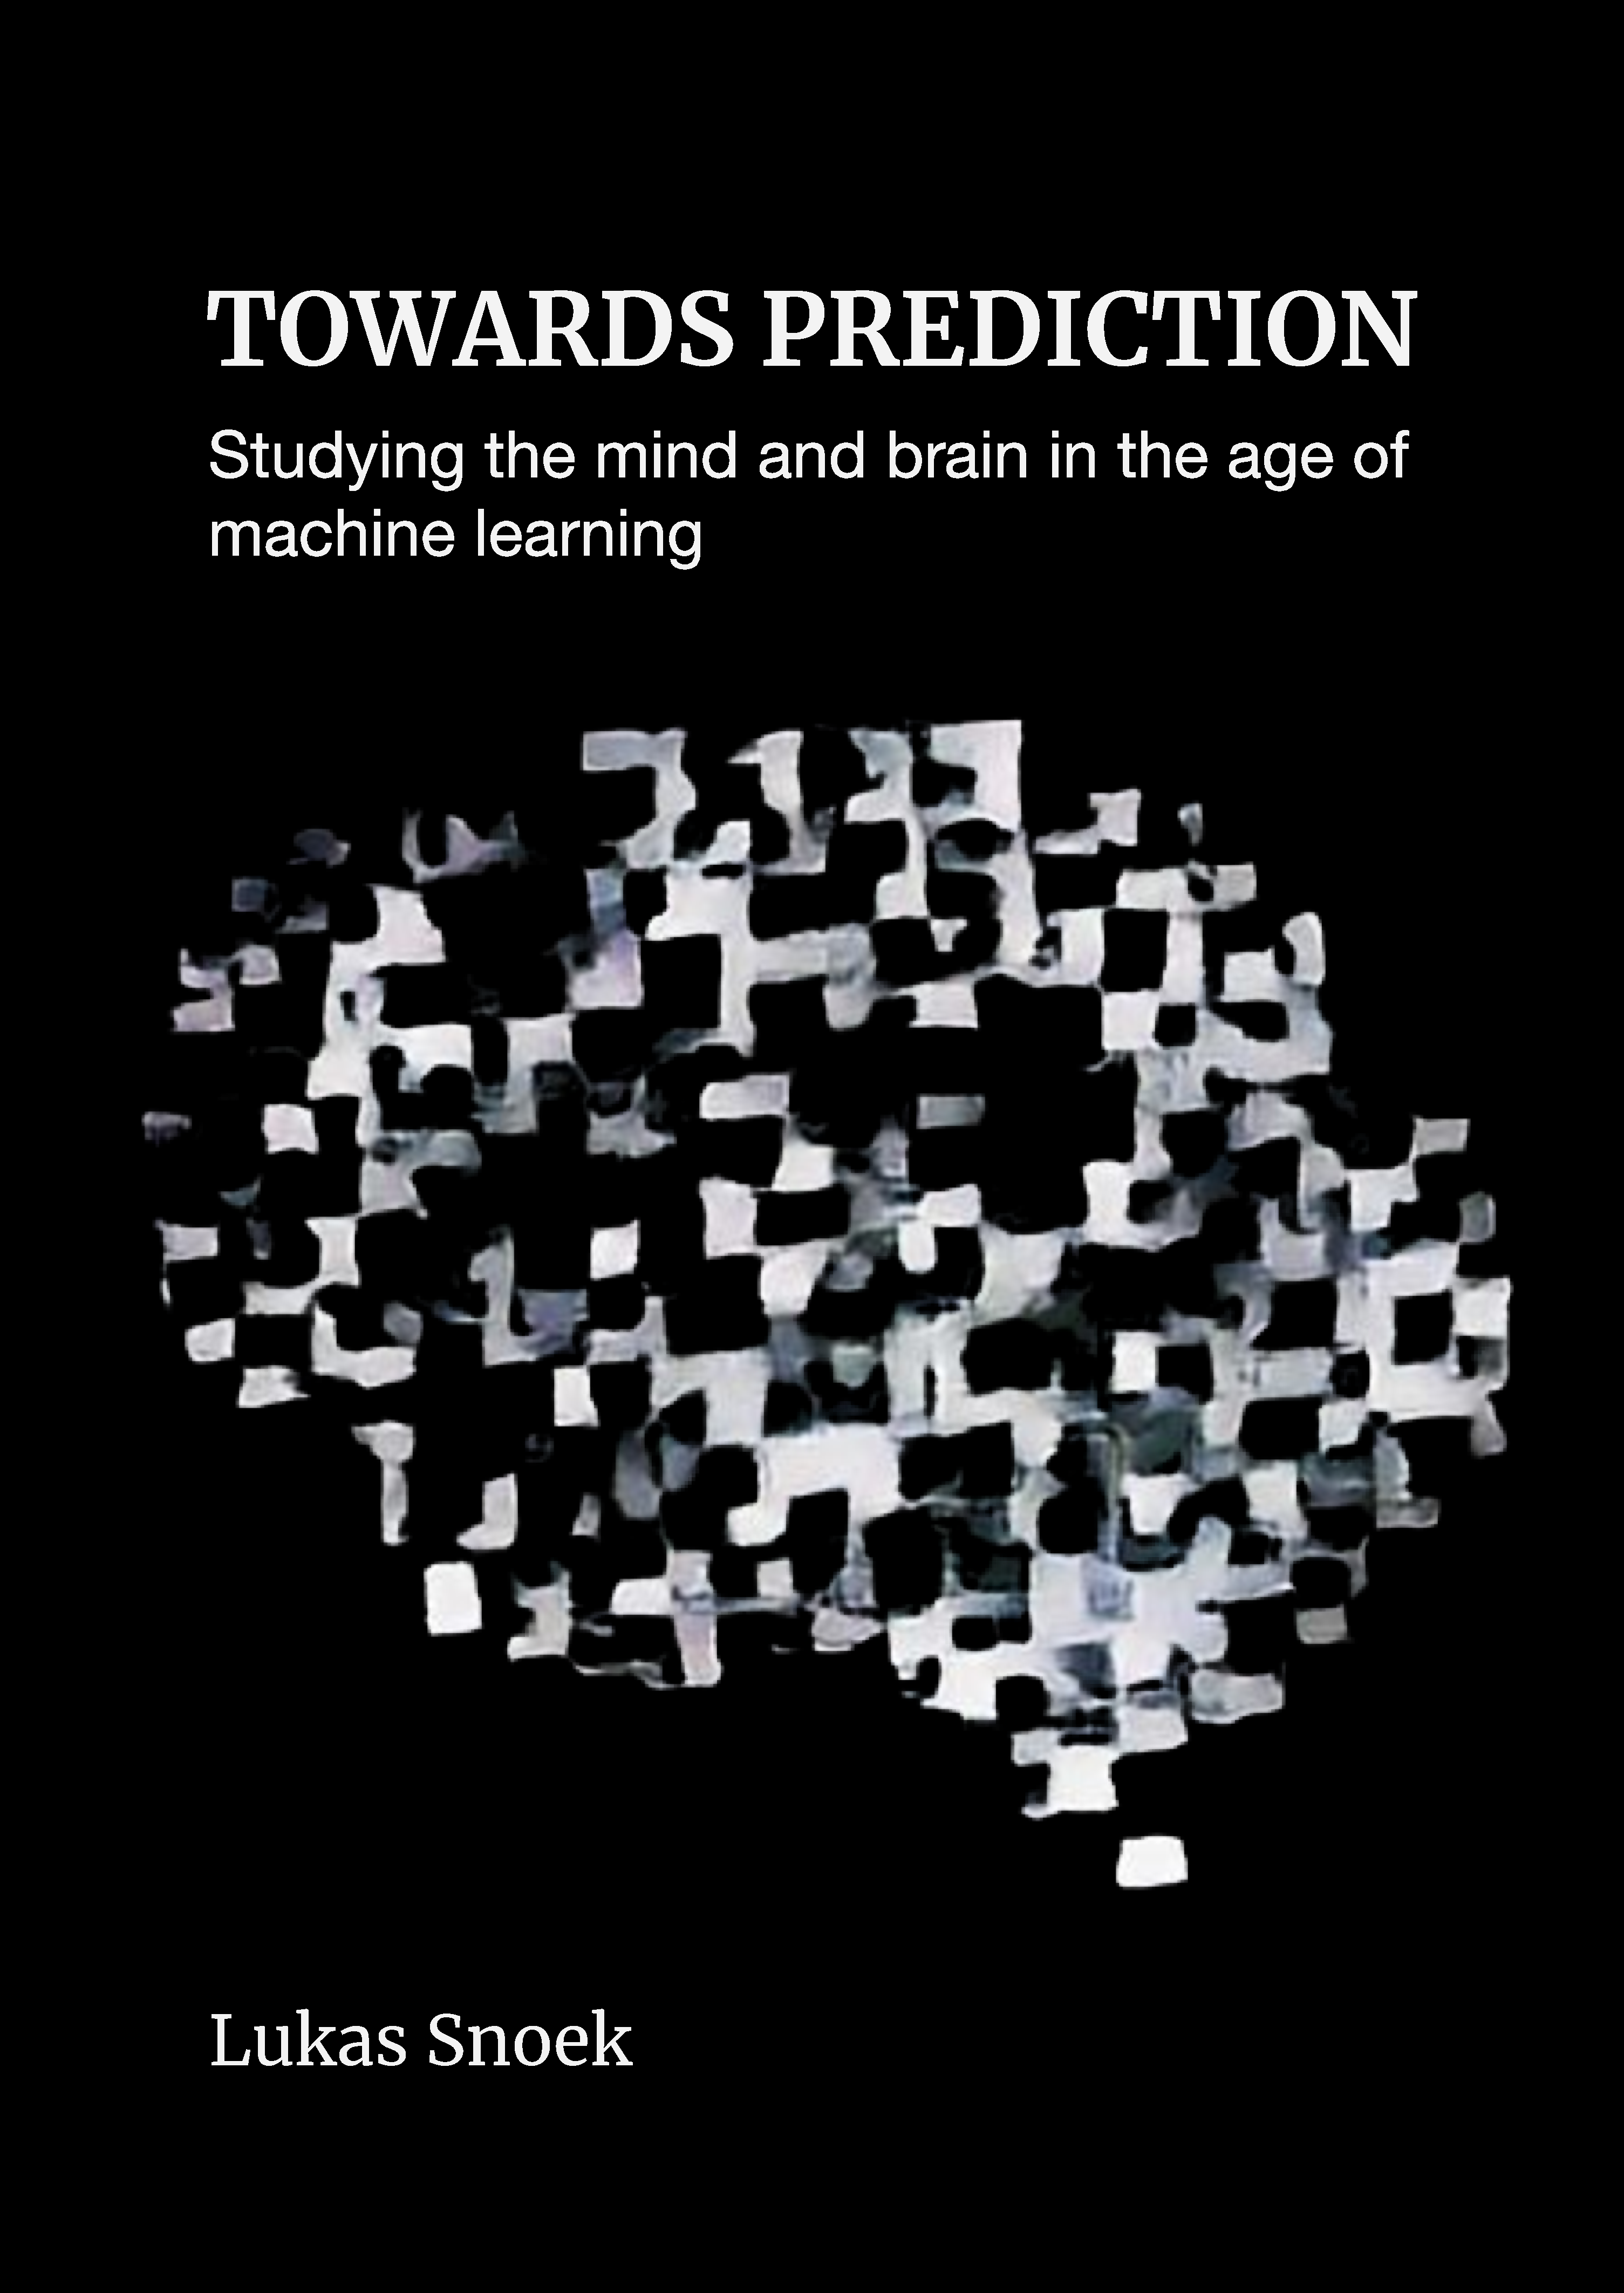
\includepdf{./cover/thesis_cover.pdf}

%% Page I: the half-title / "Franse pagina" %LCR
\frontmatter
\thispagestyle{empty}
\def\drop{.1\textheight}

\vspace*{\drop}
\begin{center}
\Huge \textsc{Towards prediction}
\end{center}

%% Page II: Colophon %LCR
\clearpage
\thispagestyle{empty}
\vspace*{\fill}
\begingroup % to change formatting only temporarily
\small
\setlength{\parskip}{\baselineskip} % add space between paragraphs
\setlength\parindent{0pt} % no indents

This thesis was typeset using (R) Markdown, \LaTeX\, \verb+bookdown+ R-package, and the \verb+bookdown+ template developed by Leon Reteig (\textit{amsterdown}).

\begin{itemize}[label={}, itemsep=0pt, partopsep=3pt, topsep=-\parskip, parsep=0pt, leftmargin=1em]
  \item ISBN: xxx-xx-xxxx-xxx-x 
  \item Printing: Ridderprint BV. 
  \item Cover art: Designed by author using a \emph{neural style transfer} (Ghiasi et al., \protect\hyperlink{ref-ghiasi2017exploring}{2017}) implementation by Reiichiro Nakano. 
\end{itemize}

\noindent An online version of this thesis is available at \url{https://lukas-snoek.com/thesis}, licensed under a CC BY.
\endgroup

%% Page III: `Title page' mandated by University of Amsterdam %LCR
\clearpage
\thispagestyle{empty}
\vspace*{\drop}
\begin{center}
\Huge\textbf{Towards prediction}\par
\vspace{\baselineskip}
\Large\textit{Studying the mind and brain in the age of machine learning}\par
\vfill % this space will be whatever is left on the page
\large \textsc{Academisch Proefschrift}\par
\vspace{\baselineskip}
\linespread{1.3}{\normalsize ter verkrijging van de graad van doctor\\
aan de Universiteit van Amsterdam\\
op gezag van de Rector Magnificus\\
prof. dr. ir. K.I.J. Maex\\ % make sure this is the current rector magnificus
\mbox{ten overstaan van een door het College voor Promoties ingestelde commissie,}\\
in het openbaar te verdedigen in de Agnietenkapel\\
op maandag 9 februari 2022, te 14.00 uur \\ }\par %
\vspace{\baselineskip}
{\large door}\par
\vspace{\baselineskip}
{\Large Lukas Snoek}\par
\vspace{\baselineskip}
{\large geboren te Hoevelaken}
\end{center}

%% Page IV: info on thesis committee %LCR
\clearpage
\thispagestyle{empty}
\noindent\textbf{Promotiecommissie:}\\
\\
\noindent\begin{tabular}{@{}lll}

Promotor:
&  dr. H.S. Scholte & Universiteit van Amsterdam\\

Copromotor:
&  dr. S. Oosterwijk & Universiteit van Amsterdam\\

\\
Overige leden:
&  prof. dr. B.U. Forstmann & Universiteit van Amsterdam\\
&  prof. dr. A.H. Fischer & Universiteit van Amsterdam\\
&  prof. dr. C. Keysers & Universiteit van Amsterdam\\
&  prof. dr. P.G. Schyns & The University of Glasgow\\
&  prof. dr. R.W. Goebel & Universiteit Maastricht\\
&  prof. dr. D. Borsboom & Universiteit van Amsterdam\\
\end{tabular}\\

\noindent Faculteit: Faculteit der Maatschappij- en Gedragswetenschappen

%% Page V (dedication)  % LS
\clearpage
\vspace*{\fill}
\begin{center}
\begin{minipage}{.6\textwidth}
\centerline{\emph{\Large Voor pap}}
\end{minipage}
\end{center}
\vfill % equivalent to \vspace{\fill}
\cleardoublepage

%%%%%%%%%%%%%%%%%%


\clearpage
\pagestyle{empty}
{
\hypersetup{linkcolor=black}
\setcounter{tocdepth}{1}
\tableofcontents
}
\pagestyle{\defstyle}
\mainmatter
\hypertarget{general-introduction}{%
\chapter{Introduction}\label{general-introduction}}

\begin{quote}
``Science advances by playing twenty questions with nature.
The proper tactic is to frame a general question, hopefully binary,
that can be attacked experimentally. Having settled that bits-worth,
one can proceed to the next. The policy appears optimal --- one never risks much,
there is feedback from nature at every step, and progress is inevitable.
Unfortunately, the questions never seem to be really answered,
the strategy does not seem to work.''

\hfill --- Allen Newell (1973)
\end{quote}

Almost fifty years ago, the artificial intelligence pioneer and cognitive psychologist Allen Newell summarized his discontent with the field of psychology with the sentence ``you cannot play twenty questions with nature and win''. In a game of ``twenty questions'', one player thinks of a person or object and the other player attempts to guess it by asking up to twenty questions, such as ``is it a person?'', ``is he a man?''. Only questions that require a binary (yes/no) answer are allowed. Newell argued that most (cognitive) psychology research attempts to understand human behavior and cognition in a manner analogous to a game of twenty questions; that is, by repeatedly asking and trying to answer ``binary'' research questions --- such as ``Does cognition impact perception?'' and ``Are emotional facial expressions innate?'' --- researchers attempt to gradually explore and reduce the space of possible scientific explanations in the hope to, ultimately, converge on the ``the right answer''. Almost fifty years after Newell's twenty questions article, most of the research in both psychology and cognitive neuroscience still revolves around asking binary research questions about the mind and brain, framed as hypotheses that are evaluated using an ever increasingly sophisticated toolbox of statistical significance tests. Newell, however, believed that in order to gain a fundamental understanding of how the mind and brain work, we need to go beyond asking binary questions and try to investigate human behavior and cognition in all its complexity using quantitative, predictive models that implement human cognitive capacities and behaviors. I believe that this argument is still as relevant today as it was almost fifty years ago.

In this thesis, I explore a different, complementary approach to the traditional methodology of hypothesis testing used in psychology and cognitive neuroscience research. Although this alternative approach has deep roots in psychology and is thus by no means new, the version I advocate and have used in this thesis extends it with ideas and techniques from the rapidly growing field of artificial intelligence and specifically machine learning. As I will describe in more detail in the next section, the crucial difference between the ``hypothesis testing approach'' and the ``predictive approach'', as advocated by Newell, is the way they go about trying to explain and understand a particular cognitive capacity or behavior (Breiman, \protect\hyperlink{ref-Breiman2001-lf}{2001}). Although I believe that both approaches have their merits, I think that the predictive approach may be particularly promising given the increasing availability of large datasets and rapid advances in artificial intelligence and machine learning (Halevy et al., \protect\hyperlink{ref-Halevy2009-cv}{2009}; Yarkoni \& Westfall, \protect\hyperlink{ref-Yarkoni2017-om}{2017}).

This thesis features research that applies, adapts, and contributes to machine learning techniques and methods in the context of predictive models of behavior and neuroimaging data. Specifically, chapters in this thesis describe both examples of predictive models applied to neuroimaging data (chapter \ref{shared-states}) and behavior (chapter \ref{hypothesis-kernel-analysis} and \ref{static-vs-dynamic} as well as elements that facilitate and enrich the predictive modelling framework, such as the value of making datasets publicly accessible (chapter \ref{aomic}; Adjerid \& Kelley, \protect\hyperlink{ref-Adjerid2018-vs}{2018}; Poldrack \& Gorgolewski, \protect\hyperlink{ref-Poldrack2014-ov}{2014}), and a method to aid interpretation of predictive models (chapter \ref{confounds-decoding}). Note that the studies contained in this thesis do not all fall squarely in the predictive approach. For example, chapter \ref{morbid-curiosity} features a study that revolved around a confirmatory (and preregistered) hypothesis and chapter \ref{shared-states} describes a study that in fact tests a very specific hypothesis using a predictive model. In what follows, I will argue that the predictive approach represents a useful and promising way of doing research that complements the traditional hypothesis testing approach with respect to their common goal of explanation and gaining understanding of the brain and mind. But first, I will illustrate that these two approaches can be thought of as different inferences from the same model which helps to identify their relative (dis)advantages later.

\hypertarget{inference-done-differently}{%
\section{Inference done differently}\label{inference-done-differently}}

Both hypothesis testing and predictive modelling are scientific methods used in psychology and neuroscience to gain understanding of human cognition and behavior. Both approaches share an important common component: a statistical model (Breiman, \protect\hyperlink{ref-Breiman2001-lf}{2001}). Although there are many different definitions and interpretations of the term ``model'' (Kellen, \protect\hyperlink{ref-Kellen2019-af}{2019}), in this chapter, I define a statistical model as a quantitative representation of (a part of) a target system (Frigg \& Hartmann, \protect\hyperlink{ref-Frigg2020-hp}{2020}). In psychology and cognitive neuroscience, a target system may refer to a specific cognitive capacity (e.g., emotion recognition) or behavior (e.g., instrumental learning; Cummins, \protect\hyperlink{ref-Cummins2000-pk}{2000}; Rooij \& Baggio, \protect\hyperlink{ref-Van_Rooij2021-bk}{2021}). Models are used to create a quantitative description, or hypothesis, of how data within a target system may have been generated. Specifically, statistical models describe how one quantity of interest within the target system, \(y\) (the ``target variable''), may arise as a function (\(f\)) of one or more other quantities in the target system, \(X\) (the predictor variables or features), often in the presence of noise (\(\epsilon\)):

\begin{equation}
y = f(X) + \epsilon
\end{equation}

Put differently, models represent explanations of how variability in a particular aspect of the target system (\(y\)) arises as the result of a set of (causally related) features (Cummins, \protect\hyperlink{ref-Cummins2000-pk}{2000}; Kay, \protect\hyperlink{ref-Kay2017-vr}{2017}). For example, chapter \ref{hypothesis-kernel-analysis} and \ref{static-vs-dynamic} describe models that attempt to explain the emotion people see in others' facial expressions (\(y\)) as a function of a combination of facial movements (\(X_{\mathrm{mov}}\)):

\begin{align}
\mathrm{emotion} = f(X_{\mathrm{mov}}) + \epsilon
\end{align}

In principle, the function linking the predictors to the target can be any function that maps a vector of numbers (the predictors, \(X_{i}\)) to a single number (the target value, \(y_{i}\)), but almost all statistical tests as well as most predictive models in psychology and cognitive neuroscience use a variant of the general(ized) linear model (GLM; Ivanova et al., \protect\hyperlink{ref-Ivanova2021-wk}{2021}; Lindeløv, \protect\hyperlink{ref-Lindelov2019-jk}{2019}). A linear model assumes that the target variable (which we assume to be continuous for now) can be expressed as the sum of a set of features (\(X_{1}, X_{2}, \dots , X_{P}\)) weighted by a corresponding set of parameters (\(\beta_{1}, \beta_{2}, \dots , \beta_{P}\)). When the target variable is continuous, the corresponding linear model is more commonly known as a \emph{linear regression} model\footnote{In this chapter, we assume for simplicity that the target variable, \(y\), is continuous. The target variable, however, does not need to be continuous; in that case, linear models from the GLM additionally include an ``inverse link function'', \(g^{-1}\), that maps the linear combination of features to the right domain: \(y = g^{-1}(X\beta)\).}:

\begin{equation}
f(X) = \sum_{j=1}^{P}X_{j} \beta_{j}
\end{equation}

In linear models, like the linear regression model above, the parameters quantify the strength of the association between each predictor and the target variable. Model parameters are considered unknown and need to be estimated from data. Here, ``data'' refers to a specific number of observations of the target variable (\(y\)) and the predictor variables (\(X\)). There are various mathematical techniques to estimate the model parameters, including the well-known (ordinary) least squares analytical solution, iterative gradient-based methods, regularized least squares, and Bayesian parameter inference. These methods differ in how they estimate the data (or, in more technical terms, which particular function they optimize or minimize during estimation), but they all return an \emph{estimate} of the parameters of the model. These estimated parameters are often denoted with a ``hat'' (^; i.e., \(\hat{\beta}\)) to distinguish them from the true, but unknown, parameters (i.e., \(\beta\)).

After obtaining estimates of the model parameters, the model can be used to make predictions about the value of the target variable (\(y\)) given observations of the predictor variables (\(X\)):

\begin{equation}
\hat{y} = \sum_{j=1}^{P}X_{j} \hat{\beta}_{j}
\end{equation}

Like the ``hat'' is used to distinguish estimated from true parameters, the ``hat'' used in the equation above is used to distinguish a prediction (i.e., an estimate of the target variable, \(\hat{y}\)) from the true target value (\(y\)). The model predictions can be compared to the actual target values to evaluate the model's predictive accuracy (which is alternatively called ``model fit'' or simply ``accuracy''), which is usually summarized in a single number using metrics such as \(R^{2}\) (also more colloquially known as ``explained variance'').

Thus far, the specification of a (linear) model and the estimation of its parameters is common to both the traditional and the predictive approach. The crucial difference between the two approaches, at this point, is what element they treat as unknown and perform inference on. In the hypothesis testing approach, inference is performed on the estimated model parameters while in the predictive approach, inference is performed on the model's predictive accuracy (Bzdok, \protect\hyperlink{ref-Bzdok2017-li}{2017}).

This difference in their focus of inference is associated with different cultures of research which use statistical models to explain a target system in different ways (Breiman, \protect\hyperlink{ref-Breiman2001-lf}{2001}). In the traditional hypothesis testing approach, the inferences about model parameters are not meant to \emph{directly} explain (parts of) a target system. Instead, the target system is verbally described and explained by a \emph{theory} (Kellen, \protect\hyperlink{ref-Kellen2019-af}{2019}). Explanation of the system occurs via testing hypotheses about very specific aspects of the system that are implied by a theory, often in strictly confirmatory experiments (Wagenmakers et al., \protect\hyperlink{ref-Wagenmakers2012-vd}{2012}). Because such hypothesis-driven studies often use strictly controlled experiments in which the factor(s) of interest are explicitly manipulated, these studies afford \emph{causal} interpretation of the observed statistical effects (Groot, \protect\hyperlink{ref-degroot}{1961}). For example, if a particular theory about emotion (e.g., basic emotion theory) implies that certain categorical emotions should be universally recognized (Keltner et al., \protect\hyperlink{ref-Keltner2019-tm}{2019}), then statistical tests that show that people across the globe are able to distinguish these emotions above chance level (e.g., Ekman et al., \protect\hyperlink{ref-Ekman1969-pu}{1969}) corroborate this theory. The logic behind this approach is that we get an increasingly better understanding of the target system if we keep testing hypotheses implied by the corresponding theory. Or in Newell's terminology, if we just keep asking nature questions, we will at some point understand it.

Theories play a less significant role in the predictive modelling culture. Although theories may inspire particular classes of models and constrain the space of possible models (Rooij \& Baggio, \protect\hyperlink{ref-Van_Rooij2021-bk}{2021}), they do not necessarily represent (a description of) the target system itself. Instead of theories, the predictive approach uses models themselves to both describe and explain a target system (Guest \& Martin, \protect\hyperlink{ref-Guest2020-ef}{2021}). These models can be thought of as algorithmic or mechanistic hypotheses of how a particular cognitive capacity or behavior may emerge (Schyns et al., \protect\hyperlink{ref-schyns2009information}{2009}). For example, the categorical emotion model in chapter \ref{static-vs-dynamic} represents the mechanistic hypothesis that the capacity of people to infer and recognize emotions from others' faces occurs through an integration of weighted linear combinations of both facial movements and facial morphological features. Another example is illustrated in Chapter \ref{shared-states}, which describes a study in which we hypothesized that the same brain networks associated with emotion experience underlie the capacity for emotion understanding (Oosterwijk et al., \protect\hyperlink{ref-Oosterwijk2017-sc}{2017}). Using a predictive model trained on neural patterns associated with components of emotion experience, we could accurately predict emotion components associated with emotion understanding in others, which suggests that these two processes share a common neural implementation (Peelen \& Downing, \protect\hyperlink{ref-Peelen2007-ew}{2007}). Importantly, in the predictive approach, progress in terms of explanation and understanding is not achieved by binary tests of these theory-driven hypotheses, but by the exploration and development of increasingly accurate models of the target system itself (Naselaris et al., \protect\hyperlink{ref-Naselaris2011-oh}{2011}).

To be clear, although the research in this thesis often uses techniques and models from machine learning, the predictive approach should not be equated with machine learning. The origins of this approach, at least in the domain of psychology, can be traced back to the psychophysics studies in the late nineteenth century. Psychophysics studies aim to develop lawlike models of how stimulus attributes give rise to sensory experiences and rarely feature explicit hypothesis tests of model parameters (Gescheider, \protect\hyperlink{ref-Gescheider2013-zm}{2013}). Predictive, computational models also play a central role in the field of cognitive science, in which they are used as formal representations and implementations of cognitive processes (Núñez et al., \protect\hyperlink{ref-Nunez2019-lh}{2019}). While hypothesis testing has dominated much of psychology and cognitive neuroscience apart from psychophysics and cognitive science, the predictive approach has become more prominent in both psychology (Yarkoni \& Westfall, \protect\hyperlink{ref-Yarkoni2017-om}{2017}) and cognitive neuroscience (Varoquaux \& Thirion, \protect\hyperlink{ref-Varoquaux2014-su}{2014}) in recent years. Machine learning has been particularly influential in cognitive neuroscience, where it was introduced as ``pattern analysis'' (Norman et al., \protect\hyperlink{ref-norman2006beyond}{2006}), but there are many other examples of predictive approaches in psychology and cognitive neuroscience. These approaches include network analysis (Borsboom \& Cramer, \protect\hyperlink{ref-Borsboom2013-wb}{2013}) and structural equation modelling (Streiner, \protect\hyperlink{ref-Streiner2006-ze}{2006}) in psychology and system identification (Wu et al., \protect\hyperlink{ref-Wu2006-qs}{2006}), model-based cognitive neuroscience (Forstmann \& Wagenmakers, \protect\hyperlink{ref-Forstmann2015-rz}{2015}; Turner et al., \protect\hyperlink{ref-Turner2017-fi}{2017}), and encoding models in cognitive neuroscience (Holdgraf et al., \protect\hyperlink{ref-Holdgraf2017-eu}{2017}; Naselaris et al., \protect\hyperlink{ref-Naselaris2011-oh}{2011}). Although these approaches differ in the way they construct and apply models, they all emphasize predictive accuracy rather than hypothesis testing.

In sum, although the traditional and predictive approach share a core component --- a quantitative model --- they differ in what aspect of the model they use for inference. The associated research cultures implement different approaches to explain and gain understanding of a target system. As I will discuss in the next section, the predictive and hypothesis testing approach each have specific advantages and, when used in combination, can compensate for the weaknesses of the other.

\hypertarget{towards-prediction}{%
\section{Towards prediction}\label{towards-prediction}}

Scientific models come in many forms and can have many different purposes. In psychology and cognitive neuroscience, researchers use scientific models primarily to explain cognitive capacities and behaviors (Yarkoni \& Westfall, \protect\hyperlink{ref-Yarkoni2017-om}{2017}). Here I use the term ``explanation'' to be the identification of the causal components of a particular target system (ibid.). Specifically, scientific models used for hypothesis tests serve as tests of the existence of causal components implied by a particular theory. Explanation is, arguably, not the only function of scientific models. Two other functions often attributed to scientific models are prediction and exploration (Cichy \& Kaiser, \protect\hyperlink{ref-Cichy2019-zf}{2019}; Gelfert, \protect\hyperlink{ref-Gelfert2016-hd}{2016}). In what follows, I will evaluate the models from the hypothesis testing and the predictive approach on these criteria and argue that they emphasize these criteria differently.

In terms of their ability to \emph{explain}, models from the hypothesis testing approach are hard to beat. By employing carefully controlled experiments in which usually only a single factor is manipulated, hypothesis tests of models are able to clearly establish the presence of specific causal components of the target system. Moreover, these models usually contain few variables and parameters and are almost always linear, which makes for easy interpretation of the estimated causal effects. The strict experimental setup and simplicity of the models, however, leave little room for \emph{exploration} of alternative, possibly better models of the target system of phenomenon. In fact, exploration is often explicitly discouraged in the context of hypothesis testing (Wagenmakers et al., \protect\hyperlink{ref-Wagenmakers2012-vd}{2012}), which forces researchers to set up a completely new study in order to test an alternative model. Not only exploration suffers from the emphasis on explanation, but prediction as well. The very fact that most models for hypothesis testing only intend to investigate and test a very specific part of the target system results in very simple models that, arguably, cannot capture the complexity of the cognitive capacities and behaviors studied by psychologists and cognitive neuroscientists (Jolly \& Chang, \protect\hyperlink{ref-Jolly2019-lx}{2019}; Tosh et al., \protect\hyperlink{ref-Tosh2020-sf}{2020}). The result is that each individual model is usually only able to correctly \emph{predict} a fraction of the variance of the target variable. In a large sample of psychology studies, Schäfer \& Schwarz (\protect\hyperlink{ref-Schafer2019-ue}{2019}) found that the median model performance, expressed as the proportion of explained variance of the target variable, was only 12.6\% and was found to be as low as 2.5\% for purely confirmatory and preregistered studies.\footnote{Note that the original article by Schäfer \& Schwarz (\protect\hyperlink{ref-Schafer2019-ue}{2019}) reported effect size, \(r\), instead of ``variance explained'', \(R^{2}\). In analyses that are not cross-validated, the latter can be obtained by squaring the former (but see Funder \& Ozer, \protect\hyperlink{ref-Funder2019-ow}{2019}).}

A prerequisite for comparing different predictive models is that, ideally, they use the same dataset. Using the same dataset to evaluate different models not only facilitates model comparison but also facilitates incremental progress over time. The famous ImageNet dataset used in computer vision provides a striking example of the impact common datasets can have on the field (Deng et al., \protect\hyperlink{ref-Deng2009-bp}{2009}). Since 2011, the ImageNet dataset has been used in the yearly ImageNet Large Scale Visual Recognition Challenge (Russakovsky et al., \protect\hyperlink{ref-Russakovsky2015-oo}{2015}), a competition in which researchers can submit object recognition models trained and evaluated on the ImageNet dataset. In 2011, the best performing model achieved 51\% accuracy, which has improved yearly, with the best performing model in the 2021 edition achieving 91\%.6.\footnote{Retrieved from \url{https://paperswithcode.com/sota/image-classification-on-imagenet}.} In the past decade, public datasets have emerged in psychology and cognitive neuroscience as well, often motivated by the desire to improve research transparency and reproducibility (Gewin, \protect\hyperlink{ref-Gewin2016-ff}{2016}). However, few have emerged as de facto benchmarks for a given subdomain like ImageNet is for object recognition, which may be due to the fact that most of these datasets are acquired in strictly controlled experiments that strongly limit the variety of models that can be explored and thus limit their reuse (Naselaris et al., \protect\hyperlink{ref-Naselaris2021-ba}{2021}). In cognitive neuroscience, there have been some notable exceptions, which include the Natural Scenes Database (Allen et al., \protect\hyperlink{ref-Allen2021-zd}{2021}) and the Naturalistic Neuroimaging Database (Aliko et al., \protect\hyperlink{ref-Aliko2020-ry}{2020}), both with the goal to facilitate the development of models for real-world vision. In Chapter \ref{aomic}, I describe our effort to release a large, richly annotated dataset to the public domain (Snoek et al., \protect\hyperlink{ref-Snoek2021-jx}{2021}). This dataset, the Amsterdam Open MRI Collection, contains a set of multimodal MRI datasets for individual difference analyses, which colleagues and I made publicly available. Not only does the variety in data sources (MRI, physiological, demographic, and psychometric data) allow for the development of a wide variety of novel models, it can also be used to evaluate the generalizability of existing models (see e.g.~Ngo et al., \protect\hyperlink{ref-Ngo2021-kf}{2021}).

The predictive accuracy of predictive models trained on large, observational datasets, however, does not come for free. One major disadvantage of the predictive approach is that the mechanisms their models represent may not represent the actual mechanisms underlying human cognition and behavior. In other words, complex models may represent what the philosopher Daniel Dennett called ``cognitive wheels'': useful inventions that may solve practical problems, but just like wheels do not occur in nature, do not reflect the true mechanisms underlying human cognitive capacities and behaviors (Dennett, \protect\hyperlink{ref-Dennett2006-el}{2006}; see also Maas et al., \protect\hyperlink{ref-Van_der_Maas2021-rx}{2021}). A famous example of a cognitive wheel is the finding that state-of-the-art object recognition models seem to rely more on the texture than the shape of the object (Geirhos et al., \protect\hyperlink{ref-Geirhos2020-af}{2020}; Xu et al., \protect\hyperlink{ref-xu2018deeper}{2018}), which seems to be the other way around in humans (Baker et al., \protect\hyperlink{ref-baker2018deep}{2018}). Relatedly, models used in artificial intelligence seem to be extremely sensitive to spurious, non-causal relationships (Geirhos et al., \protect\hyperlink{ref-Geirhos2020-af}{2020}). A famous example of this issue is the observation that a model trained on X-ray data to predict pneumonia diagnosis in fact used text annotations included in the X-ray images rather than the images themselves (Zech et al., \protect\hyperlink{ref-Zech2018-bq}{2018}). These limitations have led to the critique that using complex predictive models to explain and understand a target system, especially when using highly non-linear models as is common in many artificial intelligence applications, is like trading in one black box for another (Kay, \protect\hyperlink{ref-Kay2017-vr}{2017}). Indeed, given the definition of ``explanation'' as identification of causal components of a target system, it is hard to argue that predictive models by themselves explain anything.

It is fair to say predictive models, by themselves, are not sufficient as a satisfactory explanation of a target system, but this is not an insurmountable issue. I would argue that the construction and evaluation of a predictive model is only the first step; the second step would be to gain insight into the mechanism that is learned by the model (Cichy \& Kaiser, \protect\hyperlink{ref-Cichy2019-zf}{2019}). In this second step, the models are treated as concrete representations of the target system that can be manipulated, experimented with, and picked apart in order to gain insights into its mechanism --- not unlike model organisms in animal research (Scholte, \protect\hyperlink{ref-Scholte2018-he}{2018}). In both the machine learning community and the psychology and cognitive neuroscience community, techniques have been developed to gain insight into the mechanisms of predictive models. One common technique is to selectively manipulate specific model components, such as parameters or intermediate stimulus representations, to test whether these manipulations lead to similar changes in behavior in models and humans (e.g., Seijdel et al., \protect\hyperlink{ref-Seijdel2020-ff}{2020}). A related technique is to selectively manipulate the input to the model instead of manipulating the model itself. Chapter \ref{confounds-decoding} outlines such a method that can be used to control for specific stimulus features (``confounds'') in predictive models applied to neuroimaging data (see also Dinga et al., \protect\hyperlink{ref-Dinga2020-si}{2020}), which can prevent models from learning spurious relationships. Another technique to increase the evidence for a ``valid'' model (rather than a cognitive wheel) is to show that key components of the model have plausible neural correlates (Güçlü \& Gerven, \protect\hyperlink{ref-Guclu2015-qj}{2015}; Kriegeskorte et al., \protect\hyperlink{ref-kriegeskorte2008representational}{2008}; Yamins et al., \protect\hyperlink{ref-yamins2014performance}{2014}) or to directly constrain models with neural data (Turner et al., \protect\hyperlink{ref-Turner2017-fi}{2017}). The underlying idea of applying these different techniques is that explanation and understanding of a target system is not something that is achieved by experiments on the target system directly, but with experiments on the models that represent them (Cichy \& Kaiser, \protect\hyperlink{ref-Cichy2019-zf}{2019}).

Even though some of the weaknesses of the predictive approach can be mitigated, this does not mean that hypothesis testing should be abandoned. I believe that hypothesis testing remains and will remain an important tool in psychology and cognitive neuroscience and that there are plenty of scenarios in which hypothesis testing should in fact be preferred. First, if the goal is not to provide explanations and gain understanding of some target system, but to test an intervention, then hypothesis testing is an appropriate method. For example, if one wants to know whether some educational intervention improves reading skills in children, then running a randomized controlled experiment and associated hypothesis test is an excellent way to answer this question. Second, hypothesis tests may be useful in providing answers to important (binary) questions that may challenge important assumptions in a particular research domain or theory. For example, Chapter \ref{morbid-curiosity} describes a neuroimaging study that investigated the neural correlates of curiosity for negative information (``morbid curiosity''; Oosterwijk et al., \protect\hyperlink{ref-Oosterwijk2020-uf}{2020}), with the preregistered hypothesis that choosing negative content activates reward-related brain regions. The confirmation of this hypothesis challenges current theories of curiosity, because the most obvious indicator of reward --- a pleasurable experience --- is missing in curiosity for negative content. Therefore, this finding may indicate that information is rewarding ``in and of itself''. Finally, phenomena established by the hypothesis testing approach may inform and constrain the development of predictive models (Borsboom et al., \protect\hyperlink{ref-Borsboom2020-xg}{2020}; Kellen, \protect\hyperlink{ref-Kellen2019-af}{2019}). An example of this feature is illustrated in Chapter \ref{static-vs-dynamic}, which describes a model that uses variance in facial morphology to predict the emotions people see in ``neutral'' faces. The development of this model was inspired by the extensive literature on the associations between factors related to variance in facial morphology (e.g., age, gender, and ethnicity) and the emotional interpretations of static, ``neutral'' faces (Hess, Adams, \& Kleck, \protect\hyperlink{ref-Hess2009-xo}{2009}). Although the predictive models were not developed to test specific effects, we actually observed (or ``replicated'' if you will) several well-known effects from the emotional expression literature, such as the visual similarity and conceptual confusion between anger and disgust expressions (Jack et al., \protect\hyperlink{ref-Jack2014-ku}{2014}).

To summarize, I believe that the predictive approach represents a useful addition to the methodological toolbelt of psychologists and cognitive neuroscientists. Given the striking progress in machine learning and artificial intelligence, I think that shifting the focus from explanation to prediction may be a promising avenue for psychology and cognitive neuroscience, but theory and hypothesis testing will remain important to constrain, inform, and test models --- an idea that will be revisited in the \protect\hyperlink{general-discussion}{general discussion}.

\hypertarget{outline-of-this-thesis}{%
\section{Outline of this thesis}\label{outline-of-this-thesis}}

Although the chapters of this thesis have been shortly introduced in the previous sections, I will shortly summarize them here for convenience.

In \textbf{chapter \ref{shared-states}}, I describe a study in which we used predictive models applied to functional MRI data, known as ``decoding models'' in the neuroimaging literature, to test an hypothesis about the shared neural basis of emotion experience and emotion understanding. To remedy the interpretational difficulties inherent to decoding analyses (and predictive models in general), \textbf{chapter \ref{confounds-decoding}} outlines a method we developed to adjust for confounds in decoding analyses which helps to rule out alternative explanations of the results. Moving away from the focus on predictive models, \textbf{chapter \ref{aomic}} is the result from our effort to publish the ``Amsterdam Open MRI Collection'' (AOMIC), a set of three large, multimodal, MRI datasets, and \textbf{chapter \ref{morbid-curiosity}} describes a confirmatory, fully pre-registered neuroimaging study on a psychological phenomenon called ``morbid curiosity''. Finally, the last two chapters return to the use of predictive models, this time in the context of facial expression perception. \textbf{Chapter \ref{hypothesis-kernel-analysis}} outlines a method we developed (``hypothesis kernel analysis'') to formalize verbal hypotheses as quantitative predictive models, which we apply to a specific set of hypotheses about how facial movements relate to categorical emotions. At last, \textbf{chapter \ref{static-vs-dynamic}} concludes this thesis with a study that compares predictive models of affective face perception based on static features (i.e., facial morphology) and dynamic features (i.e., facial movements), which shows that people integrate both sources of information in their affective inferences and experiences.

\hypertarget{shared-states}{%
\chapter{Shared states: using MVPA to test neural overlap between self-focused emotion imagery and other-focused emotion understanding}\label{shared-states}}

\chaptermark{Shared states}

\vspace*{\fill}

\begin{center}\rule{0.5\linewidth}{0.5pt}\end{center}

\small

\noindent
\emph{This chapter has been published as}: Oosterwijk, S.*, Snoek, L.*, Rotteveel, M., Barrett, L. F., \& Scholte, H. S. (2017). Shared states: using MVPA to test neural overlap between self-focused emotion imagery and other-focused emotion understanding. \emph{Social cognitive and affective neuroscience, 12}(7), 1025-1035.

* Shared first authorship
\newpage
\normalsize

\begin{abstract}
The present study tested whether the neural patterns that support imagining ``performing an action'', ``feeling a bodily sensation'' or ``being in a situation'' are directly involved in understanding \emph{other people's} actions, bodily sensations and situations. Subjects imagined the content of short sentences describing emotional actions, interoceptive sensations and situations (self-focused task), and processed scenes and focused on \emph{how} the target person was expressing an emotion, \emph{what} this person was feeling, and \emph{why} this person was feeling an emotion (other-focused task). Using a linear support vector machine classifier on brain-wide multi-voxel patterns, we accurately decoded each individual class in the self-focused task. When generalizing the classifier from the self-focused task to the other-focused task, we also accurately decoded whether subjects focused on the emotional actions, interoceptive sensations and situations of \emph{others}. These results show that the neural patterns that underlie self-imagined experience are involved in understanding the experience of other people. This supports the theoretical assumption that the basic components of emotion experience and understanding share resources in the brain.
\end{abstract} \newpage

\hypertarget{shared-states-introduction}{%
\section{Introduction}\label{shared-states-introduction}}

To navigate the social world successfully it is crucial to understand other people. But how do people generate meaningful representations of other people's actions, sensations, thoughts and emotions? The dominant view assumes that representations of other people's experiences are supported by the same neural systems as those that are involved in generating experience in the self (e.g., Gallese et al., \protect\hyperlink{ref-gallese2004unifying}{2004}; see for an overview Singer, \protect\hyperlink{ref-singer2012past}{2012}). We tested this principle of self-other neural overlap directly, using multi-voxel pattern analysis (MVPA), across three different aspects of experience that are central to emotions: actions, sensations from the body and situational knowledge.

In recent years, evidence has accumulated that suggests a similarity between the neural patterns representing the self and others. For example, a great variety of studies have shown that observing actions and sensations in other people engages similar neural circuits as acting and feeling in the self (see for an overview Bastiaansen et al., \protect\hyperlink{ref-bastiaansen2009evidence}{2009}). Moreover, an extensive research program on pain has demonstrated an overlap between the experience of physical pain and the observation of pain in other people, utilizing both neuroimaging techniques (e.g., Lamm et al., \protect\hyperlink{ref-lamm2011meta}{2011}) and analgesic interventions (e.g., Rütgen et al., \protect\hyperlink{ref-rutgen2015placebo}{2015}; Mischkowski et al., \protect\hyperlink{ref-mischkowski2016painkiller}{2016}). This process of ``vicarious experience'' or ``simulation'' is viewed as an important component of empathy (Carr et al., \protect\hyperlink{ref-carr2003neural}{2003}; Decety, \protect\hyperlink{ref-decety2011dissecting}{2011}; Keysers \& Gazzola, \protect\hyperlink{ref-keysers2014dissociating}{2014}). In addition, it is argued that mentalizing (e.g.~understanding the mental states of other people) involves the same brain networks as those involved in self-generated thoughts (Uddin et al., \protect\hyperlink{ref-uddin2007self}{2007}; Waytz \& Mitchell, \protect\hyperlink{ref-waytz2011two}{2011}). Specifying this idea further, a constructionist view on emotion proposes that both emotion experience and interpersonal emotion understanding are produced by the same large-scale distributed brain networks that support the processing of sensorimotor, interoceptive and situationally relevant information (Barrett \& Satpute, \protect\hyperlink{ref-barrett2013large}{2013}; Oosterwijk \& Barrett, \protect\hyperlink{ref-oosterwijk2014embodiment}{2014}). An implication of these views is that the representation of self- and other-focused emotional actions, interoceptive sensations and situations overlap in the brain.

Although there is experimental and theoretical support for the idea of self-other neural overlap, the present study is the first to directly test this process using MVPA across three different aspects of experience (i.e.~actions, interoceptive sensations and situational knowledge). Our experimental design consisted of two different tasks aimed at generating self- and other-focused representations with a relatively large weight given to either action information, interoceptive information or situational information.

In the \emph{self-focused} emotion imagery task (SF-task) subjects imagined performing or experiencing actions (e.g., \emph{pushing someone away}), interoceptive sensations (e.g., \emph{increased heart rate}) and situations (e.g., \emph{alone in a park at night}) associated with emotion. Previous research has demonstrated that processing linguistic descriptions of (emotional) actions and feeling states can result in neural patterns of activation associated with, respectively, the representation and generation of actions and internal states (Oosterwijk et al., \protect\hyperlink{ref-oosterwijk2015concepts}{2015}; Pulvermüller \& Fadiga, \protect\hyperlink{ref-pulvermuller2010active}{2010}). Furthermore, imagery-based inductions of emotion have been successfully used in the MRI scanner before (Oosterwijk et al., \protect\hyperlink{ref-oosterwijk2012states}{2012}; Wilson-Mendenhall et al., \protect\hyperlink{ref-wilson2011grounding}{2011}), and are seen as robust inducers of emotional experience (Lench et al., \protect\hyperlink{ref-lench2011discrete}{2011}). In the \emph{other-focused} emotion understanding task (OF-task), subjects viewed images of people in emotional situations and focused on actions (i.e., \emph{How} does this person express his/her emotions?), interoceptive sensations (i.e., \emph{What} does this person feel in his/her body) or the situation (i.e., \emph{Why} does this person feel an emotion?). This task is based on previous research studying the neural basis of emotion oriented mentalizing (Spunt \& Lieberman, \protect\hyperlink{ref-spunt2012integrative}{2012}).

With MVPA, we examined to what extent the SF- and OF-task evoked similar neural patterns. MVPA allows researchers to assess whether the neural pattern associated with one set of experimental conditions can be used to distinguish between another set of experimental conditions. This relatively novel technique has been successfully applied to the field of social neuroscience in general (e.g., Gilbert et al., \protect\hyperlink{ref-gilbert2012evaluative}{2012}; Brosch et al., \protect\hyperlink{ref-brosch2013implicit}{2013}; Parkinson et al., \protect\hyperlink{ref-parkinson2014common}{2014}), and the field of self-other neural overlap in particular. For example, several MVPA studies recently assessed whether experiencing pain and observing pain in others involved similar neural patterns (Corradi-Dell'Acqua et al., \protect\hyperlink{ref-corradi2016cross}{2016}; Krishnan et al., \protect\hyperlink{ref-krishnan2016somatic}{2016}). Although there is an ongoing discussion about the specifics of shared representation in pain based on these MVPA results (see for an overview Zaki et al., \protect\hyperlink{ref-zaki2016anatomy}{2016}), many authors emphasize the importance of this technique in the scientific study of self-other neural overlap (e.g., Corradi-Dell'Acqua et al., \protect\hyperlink{ref-corradi2016cross}{2016}; Krishnan et al., \protect\hyperlink{ref-krishnan2016somatic}{2016}).

MVPA is an analysis technique that decodes latent categories from fMRI data in terms of multi-voxel patterns of activity (Norman et al., \protect\hyperlink{ref-norman2006beyond}{2006}). This technique is particularly suited for our research question for several reasons. First of all, although univariate techniques can demonstrate that tasks activate the same brain regions, only MVPA can statistically test for shared representation (Lamm \& Majdandžić, \protect\hyperlink{ref-lamm2015role}{2015}). We will evaluate whether multivariate brain patterns that distinguish between mental events in the SF-task can be used to distinguish, above chance level, between mental events in the OF-task. Second, MVPA analyses are particularly useful in research that is aimed at examining distributed representations (Singer, \protect\hyperlink{ref-singer2012past}{2012}). Based on our constructionist framework, we indeed hypothesize that the neural patterns that will represent self- and other focused mental events are distributed across large-scale brain networks. To capture these distributed patterns, we used MVPA in combination with data-driven univariate feature selection on whole-brain voxel patterns, instead of limiting our analysis to specific regions-of-interest (Haynes, \protect\hyperlink{ref-haynes2015primer}{2015}). And third, in contrast to univariate analyses that aggregate data across subjects, MVPA can be performed within-subjects and is thus able to incorporate individual variation in the representational content of multivariate brain patterns. In that aspect within-subject MVPA is sensitive to individual differences in how people imagine actions, sensations and situations, and how they understand others. In short, for our purpose to explicitly test the assumption that self and other focused processes share neural resources, MVPA is the designated method.

We tested the following two hypotheses. First, we tested whether we could classify \emph{self-imagined} actions, interoceptive sensations and situations above chance level. Second, we tested whether the multivariate pattern underlying this classification could also be used to classify the how, what and why condition in the \emph{other-focused} task.

\hypertarget{shared-states-methods}{%
\section{Methods}\label{shared-states-methods}}

\hypertarget{shared-states-methods-subjects}{%
\subsection{Subjects}\label{shared-states-methods-subjects}}

In total, we tested 22 Dutch undergraduate students from the University of Amsterdam (14 females; M\textsubscript{age} = 21.48, s.d.\textsubscript{age} = 1.75). Of those 22 subjects, 13 subjects were tested twice in 2 sessions about 1 week apart. Half of those sessions were used for the model optimization procedure. The other half of the sessions, combined with an additional nine subjects (who were tested only once), constituted the model validation set (see Model optimization procedure section). In total, two subjects were excluded from the model validation dataset: one subject was excluded because there was not enough time to complete the experimental protocol and another subject was excluded due to excessive movement (\textgreater3 mm within data acquisition runs).

All subjects signed informed consent prior to the experiment. The experiment was approved by the University of Amsterdam's ethical review board. Subjects received 22.50 euro per session. Standard exclusion criteria regarding MRI safety were applied and people who were on psychopharmacological medication were excluded a priori.

\hypertarget{shared-states-methods-experimental-design}{%
\subsection{Experimental design}\label{shared-states-methods-experimental-design}}

\hypertarget{shared-states-methods-experimental-design-sf-task}{%
\subsubsection{Self-focused emotion imagery task}\label{shared-states-methods-experimental-design-sf-task}}

The self-focused emotion imagery task (SF-task) was created to preferentially elicit \emph{self-focused} processing of action, interoceptive or situational information associated with emotion. Subjects processed short linguistic cues that described actions (e.g., \emph{pushing someone away}; \emph{making a fist}), interoceptive sensations (e.g., \emph{being out of breath}; \emph{an increased heart rate}), or situations (e.g., \emph{alone in a park at night}; \emph{being falsely accused}) and were instructed to imagine performing or experiencing the content. The complete instruction is presented in the Supplementary Materials; all stimuli used in the SF-task are presented in Supplementary Table \ref{tab:tab-shared-states-S1}. Linguistic cues were selected from a pilot study performed on an independent sample of subjects (\emph{n} = 24). Details about this pilot study are available on request. The descriptions generated in this pilot study were used as qualitative input to create short sentences that described actions, sensations or situations that were associated with negative emotions, without including discrete emotion terms. The cues did not differ in number of words, nor in number of characters (\emph{F} \textless{} 1).

The SF-task was performed in two runs subsequent to the other-focused task using the software package Presentation (Version 16.4, \url{www.neurobs.com}). Each run presented 60 sentences on a black background (20 per condition) in a fully randomized event-related fashion, with a different randomization for each subject. Note that implementing a separate randomization for each subject prevents inflated false positive pattern correlations between trials of the same condition, which may occur in single-trial designs with short inter-stimulus intervals (Mumford et al., \protect\hyperlink{ref-mumford2014impact}{2014}). A fixed inter-trial--interval of 2 seconds separating trials; 12 null-trials (i.e.~a black screen for 8 seconds) were mixed with the experimental trials at random positions during each run (see Figure \ref{fig:fig-shared-states-1}).

\begin{figure}
\centering
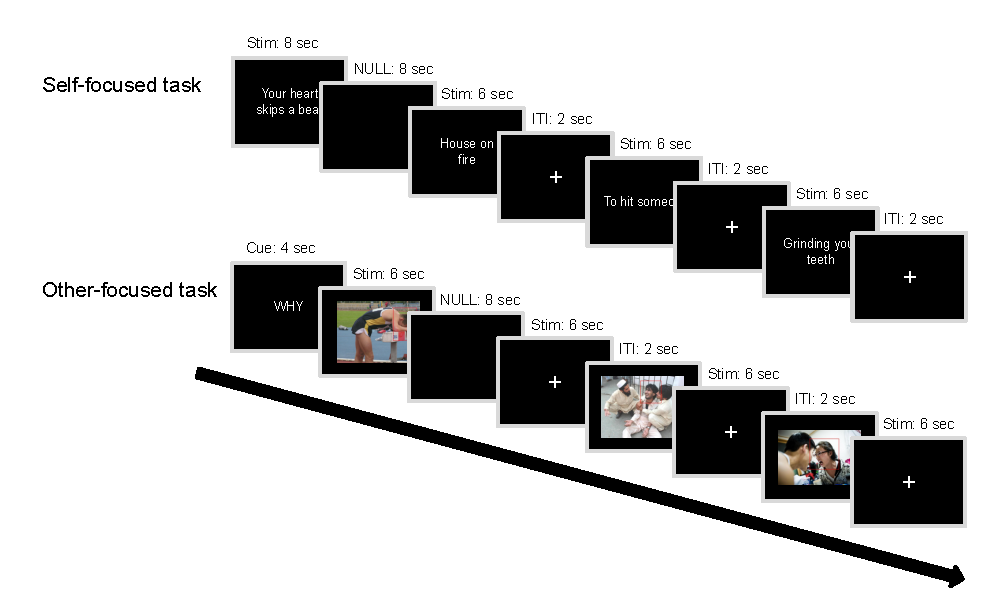
\includegraphics{_bookdown_files/shared-states-files/figures/figure_1.pdf}
\caption{\label{fig:fig-shared-states-1}Overview of the self-focused and other-focused task.}
\end{figure}

\hypertarget{shared-states-methods-experimental-design-of-task}{%
\subsubsection{Other-focused emotion understanding task}\label{shared-states-methods-experimental-design-of-task}}

The other-focused emotion understanding task (OF-task) was created to preferentially elicit \emph{other-focused} processing of action, interoceptive or situational information associated with emotion. Subjects viewed images of people in negative situations (e.g.~a woman screaming at a man, a man held at gunpoint). A red rectangle highlighted the face of the person that the subjects should focus on to avoid ambiguity in images depicting more than one person. Image blocks were preceded by a cue indicating the strategy subjects should use in perceiving the emotional state of the people in the images (Spunt \& Lieberman, \protect\hyperlink{ref-spunt2012integrative}{2012}). The cue \emph{How} instructed the subjects to identify actions that were informative about the person's emotional state (i.e., \emph{How} does this person express his/her emotions?). The cue \emph{What} instructed subjects to identify interoceptive sensations that the person could experience (i.e., \emph{What} does this person feel in his/her body). The cue \emph{Why} instructed subjects to identify reasons or explanations for the person's emotional state (i.e., \emph{Why} does this person feel an emotion?). The complete instruction is presented in the \protect\hyperlink{shared-states-supplement}{Supplementary Materials}.

Stimuli for the OF-task were selected from the International Affective Picture System database (IAPS; Lang, \protect\hyperlink{ref-lang2005international}{2005}; Lang et al., \protect\hyperlink{ref-lang1997international}{1997}), the image set developed by the Kveraga lab (\url{http://www.kveragalab.org/stimuli.html}; Kveraga et al., \protect\hyperlink{ref-kveraga2015if}{2015}) and the internet (Google images). We selected images based on a pilot study, performed on an independent sample of subjects (\emph{n} = 22). Details about this pilot study are available on request.

The OF-task was presented using the software package Presentation. The task presented thirty images on a black background in blocked fashion, with each block starting with a what, why or how cue (see Figure \ref{fig:fig-shared-states-1}). Each image was shown three times, once for each cue type. Images were presented in blocks of six, each lasting 6 seconds, followed by a fixed inter trial interval of 2 seconds. Null-trials were inserted at random positions within the blocks. Both the order of the blocks and the specific stimuli within and across blocks were fully randomized, with a different randomization for each subject.

\hypertarget{shared-states-methods-procedure}{%
\subsection{Procedure}\label{shared-states-methods-procedure}}

Each experimental session lasted about 2 hours. Subjects who underwent two sessions had them on different days within a time span of 1 week. On arrival, subjects gave informed consent and received thorough task instructions, including practice trials (see the \protect\hyperlink{shared-states-supplement}{Supplementary Materials} for a translation of the task instructions). The actual time in the scanner was 55 minutes, and included a rough 3D scout image, shimming sequence, 3-min structural T1-weighted scan, one functional run for the OF-task and two functional runs for the SF-task. We deliberately chose to present the SF-task after the OF-task to exclude the possibility that the SF-task affected the OF-task, thereby influencing the success of the decoding procedure.

After each scanning session, subjects rated their success rate for the SF-task and OF-task (see Supplementary Figure \ref{fig:fig-shared-states-S1}). In the second session, subjects filled out three personality questionnaires that will not be further discussed in this paper and were debriefed about the purpose of the study.

\hypertarget{shared-states-methods-image-acquisition}{%
\subsection{Image acquisition}\label{shared-states-methods-image-acquisition}}

Subjects were tested using a Philips Achieva 3T MRI scanner and a 32-channel SENSE headcoil. A survey scan was made for spatial planning of the subsequent scans. Following the survey scan, a 3-min structural T1-weighted scan was acquired using 3D fast field echo (TR: 82 ms, TE: 38 ms, flip angle: 8°, FOV: 240 × 188 mm, 220 slices acquired using single-shot ascending slice order and a voxel size of 1.0 × 1.0 × 1.0 mm). After the T1-weighted scan, functional T2*-weighted sequences were acquired using single shot gradient echo, echo planar imaging (TR = 2000 ms, TE = 27.63 ms, flip angle: 76.1°, FOV: 240 × 240 mm, in-plane resolution 64 × 64, 37 slices (with ascending acquisition), slice thickness 3 mm, slice gap 0.3 mm, voxel size 3 × 3 × 3 mm), covering the entire brain. For the SF-task, 301 volumes were acquired; for the OF-task 523 volumes were acquired.

\hypertarget{shared-states-methods-model-optimization-procedure}{%
\subsection{Model optimization procedure}\label{shared-states-methods-model-optimization-procedure}}

As MVPA is a fairly novel technique, no consistent, optimal MVPA pipeline has been established (Etzel et al., \protect\hyperlink{ref-etzel2011impact}{2011}). Therefore, we adopted a validation strategy in the present study that is advised in the pattern classification field (Kay et al., \protect\hyperlink{ref-kay2008identifying}{2008}; Kriegeskorte et al., \protect\hyperlink{ref-kriegeskorte2009circular}{2009}). This strategy entailed that we separated our data into an optimization dataset to find the most optimal parameters for preprocessing and analysis, and a validation dataset to independently verify classification success with those optimal parameters. We generated an optimization and validation dataset by running the SF-task and OF-task twice, in two identical experimental sessions for a set of thirteen subjects. The sessions were equally split between the optimization and validation set (see Figure \ref{fig:fig-shared-states-2}A); first and second sessions were counterbalanced between the two sets. Based on a request received during the review process, we added nine new subjects to the validation dataset. Ultimately, the optimization-set held 13 sessions and the validation-set, after exclusion of 2 subjects (see \protect\hyperlink{shared-states-methods-subjects}{Subjects} section), held 20 sessions.

\begin{figure}
\centering
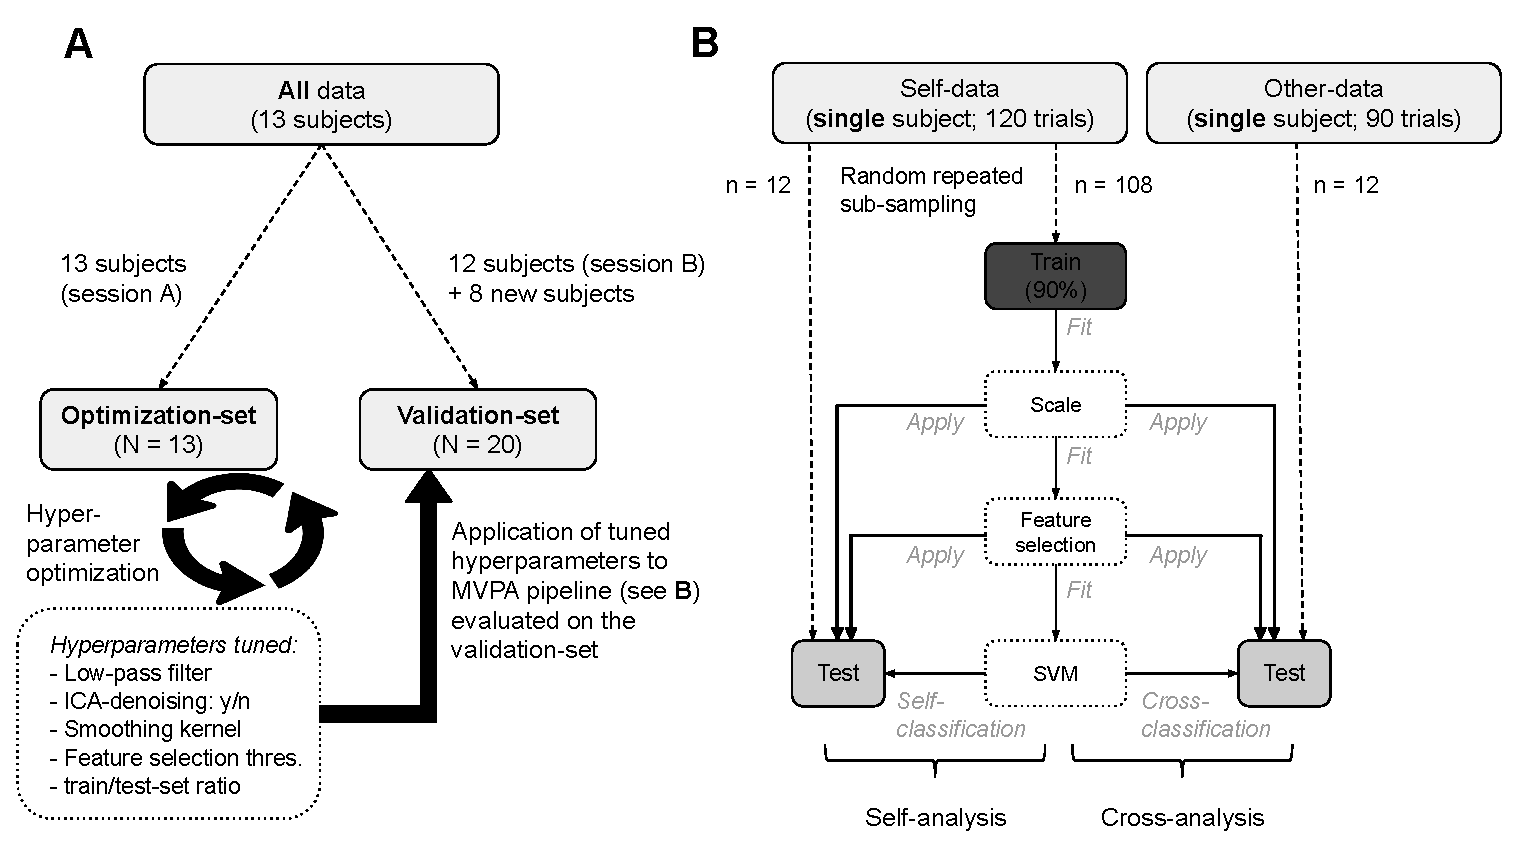
\includegraphics{_bookdown_files/shared-states-files/figures/figure_2.pdf}
\caption{\label{fig:fig-shared-states-2}Schematic overview of the cross-validation procedures. \textbf{A}) The partitioning of the dataset into an optimization-set (used for tuning of preprocessing and MVPA hyperparameters) and a validation-set (used to get a fully cross-validated, unbiased estimate of classification performance). The preprocessing and MVPA hyperparameters yielded from the optimization procedure were subsequently applied to the preprocessing and MVPA pipeline of the validation-set. \textbf{B}) The within-subject MVPA pipeline of the self- and cross-analysis implemented in a repeated random subsampling scheme with 100,000 iterations. In each iteration, 90\% of the self-data trials (i.e.~train-set) were used for estimating the scaling parameters, performing feature selection and fitting the SVM. These steps of the pipeline (i.e.~scaling, feature selection, SVM fitting) were subsequently applied to the independent test-set of both the self-data trials and the other-data trials.}
\end{figure}



In the optimization-set, we explored how different preprocessing options and the so-called `hyperparameters' in the MVPA pipeline affected the performance of the (multivariate) analyses (visualized in Figure \ref{fig:fig-shared-states-2}B; see \protect\hyperlink{shared-states-methods-mvpa-pipeline}{MVPA pipeline} subsection for more details). Thus, we performed the self- and cross-analyses \emph{on the data of the optimization set} multiple times with different preprocessing options (i.e., smoothing kernel, low-pass filter and ICA-based denoising strategies) and MVPA hyperparameter values (i.e., univariate feature selection \emph{threshold} and train/test size ratio during cross-validation). We determined the optimal parameters on the basis of classification performance, which was operationalized as the mean precision value after a repeated random subsampling procedure with 1000 iterations. A list with the results from the optimization procedure can be found in Supplementary Table \ref{tab:tab-shared-states-S2} and Supplementary Figure \ref{fig:fig-shared-states-S2}. The optimal parameters were then used for preprocessing and the self- and cross-analysis within the validation-set, in which the findings from the optimization-set were replicated. All findings discussed in the \ref{shared-states-results} section follow from the validation-set (see Supplementary Figure \ref{fig:fig-shared-states-S3} for an overview of the findings from the optimization-set).

\hypertarget{shared-states-methods-preprocessing}{%
\subsection{Preprocessing and single-trial modeling}\label{shared-states-methods-preprocessing}}

Functional and structural data were preprocessed and analyzed using FSL 5.0 (Jenkinson et al., \protect\hyperlink{ref-Jenkinson2012-ui}{2012}) and MATLAB (2012b; \url{www.mathworks.com/products/matlab}), using an in-house developed preprocessing pipeline and the parameters established in the optimization procedure. Functional data were corrected for motion (using FSL MCFLIRT) and slice timing and was spatially smoothed (5 mm isotropic kernel). After preprocessing, individual time series were modeled using a double-gamma hemodynamic response function in a single-trial GLM design using FSL's FEAT. Resulting beta values were converted to \emph{t}-values (Misaki et al., \protect\hyperlink{ref-misaki2010comparison}{2010}), constituting a whole-brain pattern of \emph{t}-values per trial. Subsequently, the data were indexed by a gray-matter mask (excluding most white-matter, CSF and brainstem voxels). Thus, the data points for the MVPA consist of whole-brain (gray matter) \emph{t}-value patterns per trial. For the optimization analyses, the data were transformed to standard space (MNI152, 2 mm) using FSL's FNIRT. To reduce computation time for the validation data, and in particular its corresponding permutation analysis, analyses on the validation dataset were performed on data in native (functional) space.

\hypertarget{shared-states-methods-mvpa}{%
\subsection{Multi-voxel pattern analysis}\label{shared-states-methods-mvpa}}

\hypertarget{shared-states-methods-mvpa-pipeline}{%
\subsubsection{MVPA pipeline}\label{shared-states-methods-mvpa-pipeline}}

Within the optimization and validation dataset, we implemented an iterated cross-validation scheme that separated the data into a train-set and a test-set (this procedure is described in more detail in the next section). Before fitting the classifier on the train-set in each iteration of the cross-validation scheme, standardization and voxel selection were estimated and applied to the train-set. Standardization ensured that each feature (i.e., voxel) had zero mean and unit variance across trials. After standardization, voxel selection was performed in each iteration on the train-set by extracting the voxels with the highest average pairwise Euclidian distance across classes, which will be subsequently referred to as a voxel's differentiation score. More specifically, differentiation scores were calculated by subtracting the mean value across trials per class from each other (i.e., action---interoception, action---situation, interoception---situation), normalizing these values across voxels (yielding ``z-scores''), and taking their absolute value. The three resulting values per voxel were averaged and the most differentiating voxels (z-score threshold: 2.3, as determined by the optimization procedure; see \protect\hyperlink{shared-states-methods-model-optimization-procedure}{Model optimization procedure} section) were extracted and used as features when fitting the classifier. Importantly, the standardization parameters (voxel mean and variance) and voxel indices (i.e.~which voxels had differentiation scores above threshold) were estimated from the train-set only and subsequently applied to the test-set to ensure independence between the train- and test-set (see Figure 2B). After standardization and voxel selection in each iteration, a support vector classifier (SVC) was fit on the train-set and cross-validated on the test-set, generating a class probability for each trial in the test-set. Our classifier of choice was the SVC implementation from the scikit-learn \texttt{svm} module (Pedregosa et al., \protect\hyperlink{ref-pedregosa2011scikit}{2011}) with a linear kernel, fixed regularization parameter (\emph{C}) of 1.0, one-vs-one multiclass strategy, estimation of class probability output (instead of discrete class prediction) and otherwise default parameters.

\hypertarget{shared-states-methods-mvpa-cv-and-bagging}{%
\subsubsection{Cross-validation scheme and bagging procedure}\label{shared-states-methods-mvpa-cv-and-bagging}}

Cross-validation of the classification analysis was implemented using a repeated random subsampling cross-validation scheme (also known as Monte Carlo cross-validation), meaning that, for each iteration of the analysis, the classification pipeline (i.e., standardization, voxel selection and SVM fitting) was applied on a random subset of data points (i.e., the train-set) and cross-validated on the remaining data (i.e., the test-set). Each trial belonged to one out of three classes: action, interoception or situation. Following the results from the parameter optimization process, we selected four trials per class for testing, amounting to 12 test-trials per iteration.

Per iteration, the classifier was fit on the train-set from the SF-data. Subsequently, this classifier was cross-validated on 12 test SF-trials (test-set ``self-analysis'') and 12 test OF-trials (test-set ``cross-analysis''; see Figure 2B). This process was subsequently iterated 100 000 times to generate a set of class distributions for each trial. After all iterations, the final predicted class of each trial was determined by its highest summed class probability across iterations (also known as ``soft voting''; see Supplementary Figure \ref{fig:fig-shared-states-S4}). This strategy of a random sub-sampling cross-validation scheme in combination with majority (soft) voting is more commonly known as ``bagging'' (Breiman, \protect\hyperlink{ref-breiman1996bagging}{1996}). An important advantage of bagging is that it reduces model overfitting by averaging over an ensemble of models, which is especially useful for multi-voxel pattern analyses because fMRI data is known to display high variance (Varoquaux, \protect\hyperlink{ref-Varoquaux2018-uo}{2018}).

After generating a final prediction for all trials using the soft voting method, we constructed confusion matrices for both the self- and cross-analysis. In each raw confusion matrix with prediction counts per class, cells were normalized by dividing prediction counts by the sum over rows (i.e., the total amount of predictions per class), yielding precision-scores (also known as positive predictive value). In other words, this metric represents the ratio of true positives to the sum of true positives and false positives (see Supplementary Figure \ref{fig:fig-shared-states-S5} for a description of the results expressed as \emph{recall} estimates, or the ratio of true positives to the total number of samples in that class). This classification pipeline generated subject-specific confusion matrices that were subsequently averaged to generate the final classification scores.

\hypertarget{shared-states-methods-mvpa-statistical-evaluation}{%
\subsubsection{Statistical evaluation}\label{shared-states-methods-mvpa-statistical-evaluation}}

To evaluate the statistical significance of the observed average precision-scores in the confusion matrices, we permuted the original self- and cross-analysis 1300 times per subject with randomly shuffled class labels, yielding 1300 confusion matrices (with precision-scores). We then averaged the confusion matrices across subjects, yielding 1300 permuted confusion matrices reflecting the null-distribution of each cell of the matrix (which is centered around chance level classification, i.e., 33\%). For each cell in the diagonal of the observed confusion matrix, \emph{p}-values were calculated as the proportion of instances of values in the permuted matrix which were higher than the values in the observed matrix (Nichols \& Holmes, \protect\hyperlink{ref-nichols2002nonparametric}{2002}). To correct for multiple comparisons, \emph{p}-values were tested against a Bonferroni-corrected threshold. The distribution of precision-scores and the relationship between precision-scores in the self- and cross-analysis is reported in Supplementary Figure \ref{fig:fig-shared-states-S6}.

\hypertarget{shared-states-methods-mvpa-spatial-representation}{%
\subsubsection{Spatial representation}\label{shared-states-methods-mvpa-spatial-representation}}

To visualize the classifier feature weights, we plotted the absolute feature weights averaged over iterations, subjects and pairwise classifiers (action \emph{vs} interoception, action \emph{vs} situation, interoception \emph{vs} situation) that underlie our multiclass classification analysis. We chose to visualize the spatial representation of our model by plotting the average absolute feature weights, because the absolute value of feature weights in linear SVMs can be interpreted as how important the weights are in constructing the model's decision hyperplane (Ethofer et al., \protect\hyperlink{ref-ethofer2009decoding}{2009}; Guyon et al., \protect\hyperlink{ref-guyon2002gene}{2002}; Stelzer et al., \protect\hyperlink{ref-stelzer2014prioritizing}{2014}). To correct for a positive bias in plotting absolute weights, we ran the main classification analysis again with permuted labels to extract the average absolute feature weights that one would expect by chance. Subsequently, a voxel-wise independent \emph{t}-test was performed for all feature weights across subjects, using the average permuted feature weights as the null-hypothesis, yielding an interpretable \emph{t}-value map (see the supplementary code notebook on our Github repository for computational details).

\hypertarget{shared-states-methods-additional-analyses}{%
\subsection{Additional analyses}\label{shared-states-methods-additional-analyses}}

In addition to the self-analysis and the self-to-other cross-analysis presented in the main text, we also performed a within-subjects other-to-self cross-analysis (see for a similar approach Corradi-Dell'Acqua et al., \protect\hyperlink{ref-corradi2016cross}{2016}) and a between-subjects self-analysis and self-to-other cross-analysis. These analyses forward largely similar results as the analyses presented in the main text. Due to space constraints, we present these additional analyses in the \protect\hyperlink{shared-states-supplement}{Supplementary Materials}. Supplementary Figure \ref{fig:fig-shared-states-S7} represents confusion matrices with precision and recall estimates for the other-to-self cross-analysis. Supplementary Figure \ref{fig:fig-shared-states-S8} presents the results of MVPA analyses using condition-average voxel patterns across subjects instead of single-trial patterns within subjects.

\hypertarget{shared-states-methods-univariate-analysis}{%
\subsection{Univariate analysis}\label{shared-states-methods-univariate-analysis}}

To be complete, we also report a set of univariate analyses performed on the SF-task and the OF-task data. The univariate analyses were performed on the validation dataset, and were subject to the same preprocessing steps as the MVPA analysis, except that we did not model each trial, but each condition as a separate regressor. The group-level analysis was performed with FSL's FLAME1 option. To examine differences in neural activity between conditions, we calculated contrasts between the three classes in the SF-task (self-action \emph{vs} self-interoception; self-action \emph{vs} self-situation and self-interoception \emph{vs} self-situation) and the three classes in the OF-task (other-action \emph{vs} other-interoception; other-action \emph{vs} other-situation and other-interoception \emph{vs} other-situation). We report clusters that were corrected using cluster-correction with a voxel-wise threshold of 0.005 (\emph{z} = 2.7) and a cluster-wise \emph{p}-value threshold of 0.05.

\hypertarget{shared-states-methods-code-availability}{%
\subsection{Code availability}\label{shared-states-methods-code-availability}}

The MVPA-analysis and subsequent (statistical) analyses were implemented using custom Python scripts, which depend heavily on the skbold package, a set of tools for machine learning analyses of fMRI data developed in-house (see \url{https://github.com/lukassnoek/skbold}). The original scripts were documented and are hosted at the following Github repository: \url{https://github.com/lukassnoek/SharedStates}.

\hypertarget{shared-states-results}{%
\section{Results}\label{shared-states-results}}

\hypertarget{shared-states-results-mvpa}{%
\subsection{Multi-voxel pattern analysis}\label{shared-states-results-mvpa}}

The analyses of the SF-task demonstrated that voxel patterns reflecting imagined self-focused actions, interoceptive sensations and situations associated with emotion could be decoded accurately for each individual class (all \emph{p} \textless{} 0.001, see Figure \ref{fig:fig-shared-states-3}). Furthermore, when we generalized the classifier based on the SF-task to the data from the OF-task (i.e.~cross-analysis), we found that neural representations of emotional actions, interoceptive sensations and situations of others could also be reliably decoded above chance (all \emph{p} \textless{} 0.001; see Figure \ref{fig:fig-shared-states-3}). Supplementary Table \ref{tab:tab-shared-states-S3} presents mean precision-scores across classes for each subject separately. As predicted, our findings demonstrate that \emph{self-imagined} actions, interoceptive sensations and situations are associated with distinct neural patterns. Furthermore, and as predicted, our findings demonstrate that the patterns associated with self-imagined actions, sensations and situations can be used to decode \emph{other-focused} actions, interoceptive sensations and situations (see Supplementary Figure \ref{fig:fig-shared-states-S7} for the complementary other-to-self cross-analysis).

\begin{figure}
\centering
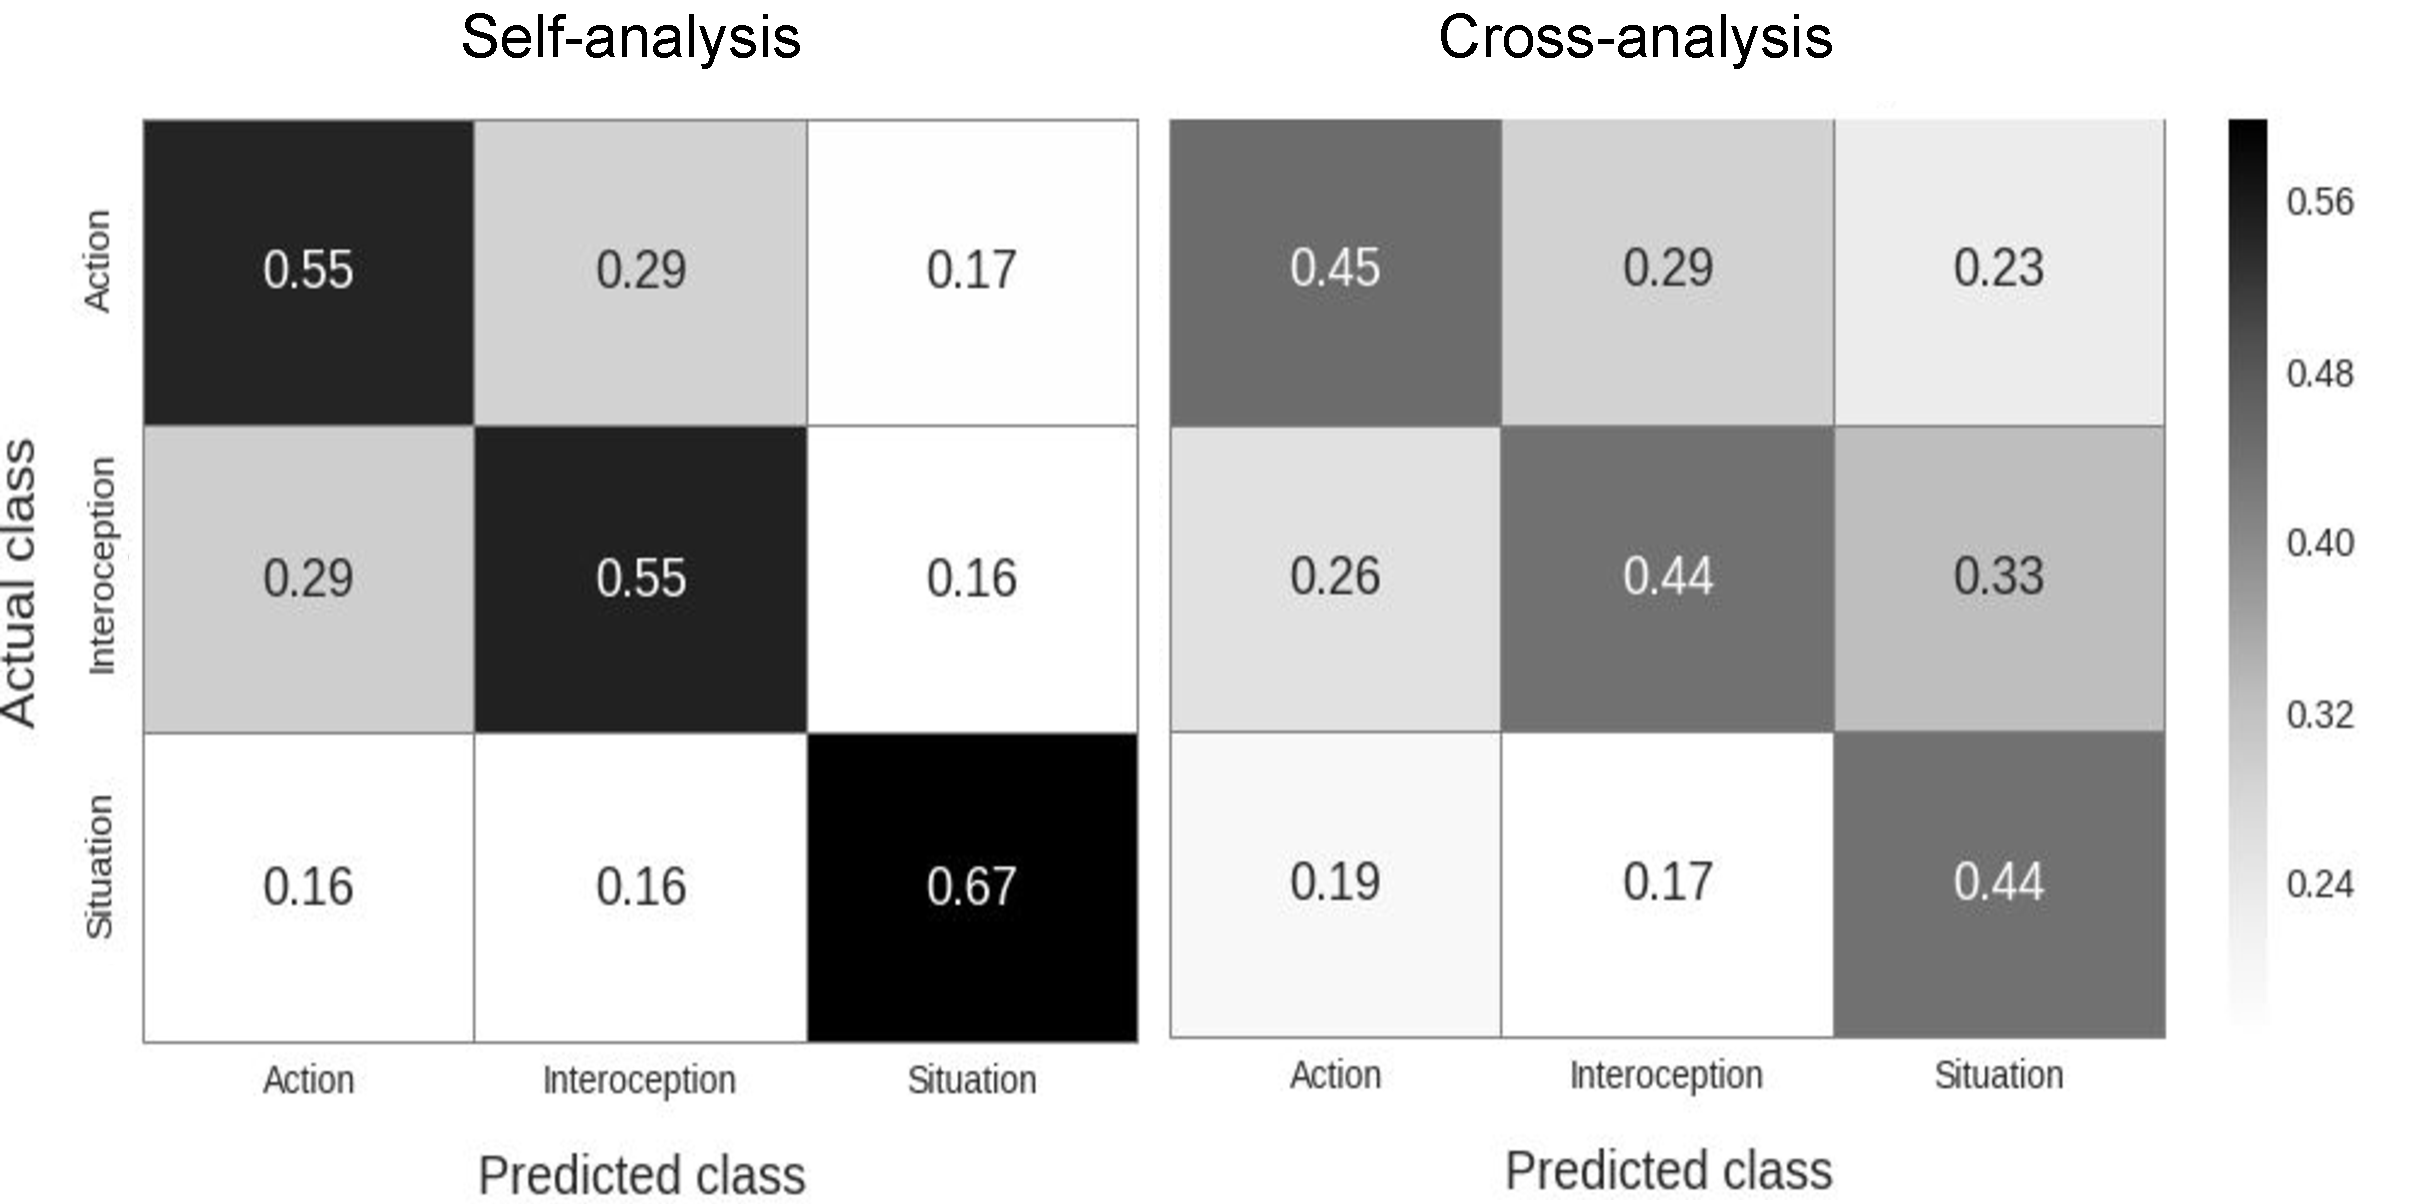
\includegraphics{_bookdown_files/shared-states-files/figures/figure_3.pdf}
\caption{\label{fig:fig-shared-states-3}Confusion matrices for the self- (left diagram) and cross-analysis (right diagram). Values indicate precision-scores, representing the proportion of true positives given all predictions for a certain class. Note that action and interoception columns in the cross-analysis confusion matrix do not add up to 1, which is caused by the fact that, for some subjects, no trials were predicted as action or interoception, rendering the calculation of precision ill-defined (i.e., division by zero). In this case, precision scores were set to zero.}
\end{figure}



To visualize which neural regions were involved in the successful decoding of the three classes in the OF-task and SF-task, we display in Figure \ref{fig:fig-shared-states-4} the averaged absolute values of the SVM feature weights. Note that Figure \ref{fig:fig-shared-states-4} only displays one feature map, as both the self and cross-analysis depend on the same model. Regions displaying high and consistent feature weights across subjects were frontal pole (including parts of the dorsomedial prefrontal cortex and ventromedial prefrontal cortex), orbitofrontal cortex (OFC), inferior frontal gyrus (IFG), superior frontal gyrus (SFG), middle frontal gyrus (MFG), insular cortex, precentral gyrus, postcentral gyrus, posterior cingulate cortex/precuneus, superior parietal lobule (SPL), supramarginal gyrus (SMG), angular gyrus (AG), middle temporal gyrus (MTG), temporal pole (TP), lateral occipital cortex (lOC) and occipital pole (see Supplementary Table \ref{tab:tab-shared-states-S4} for an overview of all involved regions).

\begin{figure}
\centering
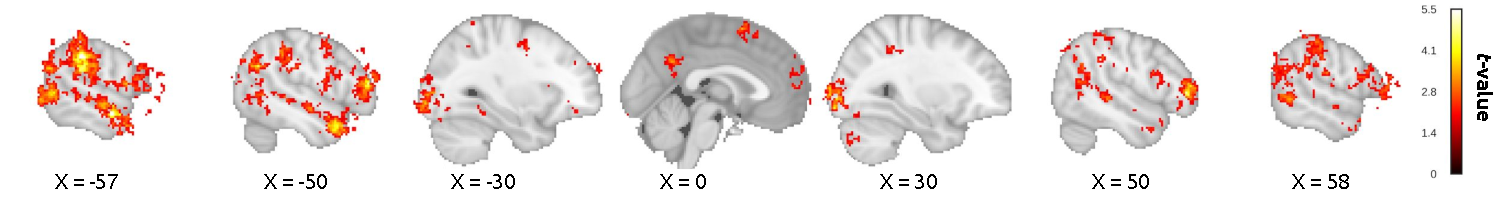
\includegraphics{_bookdown_files/shared-states-files/figures/figure_4.pdf}
\caption{\label{fig:fig-shared-states-4}Uncorrected \emph{t}-value map of average feature weights across subjects; \emph{t}-values were calculated by dividing the average absolute feature weights, which was corrected for positive bias by subtracting the mean permuted absolute weight across all iterations, by the standard error across subjects. Only voxels belonging to clusters of 20 or more voxels are shown.}
\end{figure}



\hypertarget{shared-states-results-univariate}{%
\subsection{Univariate analyses}\label{shared-states-results-univariate}}

Figure \ref{fig:fig-shared-states-5} displays the pattern of neural activity revealed by univariate contrasts between the three different classes in the SF-task and the OF-task. For the sake of brevity, we summarize the most relevant univariate results here. Please see the \protect\hyperlink{shared-states-supplement}{Supplementary Materials} and the study's Github repository for an overview of all clusters.

\begin{figure}
\centering
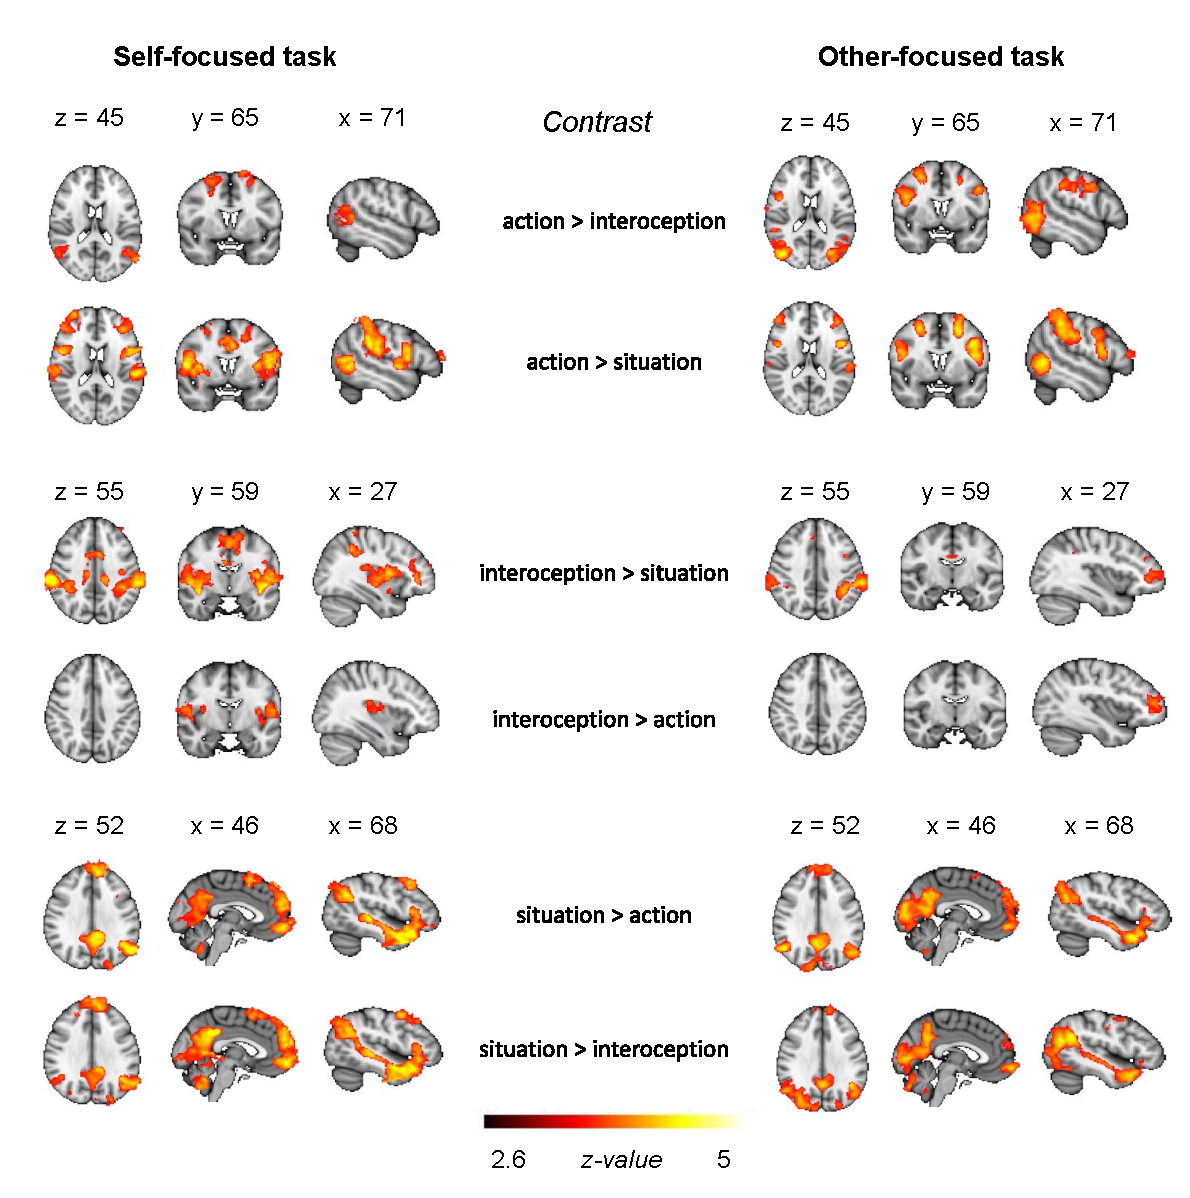
\includegraphics{_bookdown_files/shared-states-files/figures/figure_5.pdf}
\caption{\label{fig:fig-shared-states-5}Univariate contrasts for the self-focused and other-focused task.}
\end{figure}

In the SF-task, action was associated with increased involvement of the MFG, SFG, AG, SMG, lOC and middle temporal gyrus (temporo-occipital) when compared with interoception, and increased involvement of the IFG, MFG, SFG, anterior cingulate cortex (ACC), supplementary motor area (SMA), precentral gyrus, postcentral gyrus, insular cortex, SMG, SPL, lOC and middle temporal gyrus (temporo-occipital) when compared with situation. Interoception was associated with increased involvement of the insular cortex, precentral gyrus, postcentral gyrus and central operculum when compared with action, and increased involvement of the insular cortex, central operculum, parietal operculum, IFG, frontal pole, ACC, SMA, precentral gyrus, postcentral gyrus, SMG, SPL and putamen when compared with situation. The situation \emph{vs} action contrast and the situation \emph{vs} interoception contrast forwarded clusters in similar regions, including the temporal pole, superior/middle temporal gyrus, IFG, SFG, frontal pole, medial prefrontal cortex (mPFC), OFC, precuneus, posterior cingulate cortex (PCC), lOC, fusiform gyrus, hippocampus and lingual gyrus.

In the OF-task, action was associated with increased involvement of the IFG, MFG, SFG, precentral gyrus, postcentral gyrus, SMG, SPL, middle/inferior temporal gyrus (temporo-occipital), lOC and fusiform gyrus, when compared with interoception, and increased involvement of the IFG, MFG, SFG, frontal pole, precentral gyrus, postcentral gyrus, SMG, SPL, middle/inferior temporal gyrus (temporo-occipital) and lOC, when compared with situation. Interoception was associated with increased involvement of the left frontal pole when compared with action, and increased involvement of the SMG, SPL, precentral gyrus, postcentral gyrus, PCC, IFG and frontal pole, when compared with situation. The situation \emph{vs} action contrast and the situation \emph{vs} interoception contrast forwarded clusters in similar regions, including the temporal pole, superior/middle temporal gyrus, frontal pole, mPFC, PCC, precuneus, AG, lOC, occipital pole, fusiform gyrus and lingual gyrus.

\hypertarget{shared-states-discussion}{%
\section{Discussion}\label{shared-states-discussion}}

In this study, we investigated the neural overlap between self-focused emotion imagery and other-focused emotion understanding using a decoding approach. The results confirmed our hypothesis that other-focused representations of emotion-related actions, bodily sensations and situations can be decoded from neural patterns associated with accessing similar sources of information in a self-focused task. This cross-classification was successful even though the tasks employed different stimulus materials and instructions. Thus, the observed neural overlap between the underlying processes in the SF-task and OF-task cannot be attributed to similarities in stimulus dimensions or task instructions. Rather, we conclude from our findings that emotion experience and emotion understanding have basic psychological processes in common.

Although we could successfully classify the interoception class in the SF-task (across both datasets), and in the OF-task in the validation dataset, we were not able to successfully classify the interoception class in the OF-task in the optimization dataset. Furthermore, although precision and recall metrics demonstrated similar results for the action and situation cross-classification in the validation dataset, these metrics demonstrated different results for the classification of the interoception class (see Supplementary Figure \ref{fig:fig-shared-states-S5}). This difference was partly driven by the fact that trials were very infrequently classified as interoception in the cross-classification analysis. The finding that subjects reported lower success rates for the \emph{what} trials in which they were asked to identify interoceptive sensations in other people than for the \emph{how} (action) and \emph{why} (situation) trials may point to a possible explanation for the inconsistent findings regarding interoception. Although speculative, it may be relatively easy to recognize (and represent) interoceptive sensations when they are described in words (as in the SF-task), but relatively hard to deduce these sensations when only diffuse cues about someone's internal state are available (e.g.~posture, frowning facial expression, as in the OF-task).

An exploration of the spatial characteristics of the distributed neural pattern associated with successful decoding of the SF-task and OF-task revealed regions that are commonly active during self- and other-focused processing. First, we found that successful classification was associated with voxels in the precentral gyrus, IFG, SMA and SPL. These same regions were also revealed by the univariate analyses, in particular for the action and interoception classes. These regions are part of the so-called ``mirror'' network, which is argued to support both action planning and action understanding (Bastiaansen et al., \protect\hyperlink{ref-bastiaansen2009evidence}{2009}; Gallese et al., \protect\hyperlink{ref-gallese2004unifying}{2004}; Spunt \& Lieberman, \protect\hyperlink{ref-spunt2012integrative}{2012}; Van Overwalle \& Baetens, \protect\hyperlink{ref-van2009understanding}{2009}). Furthermore, we found that successful classification was associated with voxels in the lateral occipital cortex and fusiform gyrus, which have been linked in the literature to the processing of both concrete and abstract action (Wurm \& Lingnau, \protect\hyperlink{ref-wurm2015decoding}{2015}) and the (visual) processing of emotional scenes, faces and bodies (Gelder et al., \protect\hyperlink{ref-de2010standing}{2010}; Sabatinelli et al., \protect\hyperlink{ref-sabatinelli2011emotional}{2011}). The univariate analyses demonstrated activity in the lOC and the fusiform gyrus in particular for the situation class, both when subjects viewed images of other people in emotional situations, and when subjects imagined being in an emotional situation themselves.

Second, we found that successful classification was associated with voxels in regions associated with somatosensory processing (postcentral gyrus) and the representation of interoceptive sensations (insular cortex, see Craig \& Craig, \protect\hyperlink{ref-craig2009you}{2009}; Medford \& Critchley, \protect\hyperlink{ref-medford2010conjoint}{2010}). Univariate analyses of the SF-task also demonstrated involvement of these regions for both the action and interoception classes. This pattern of activation is consistent with embodied cognition views that propose that thinking about or imagining bodily states is grounded in simulations of somatosensory and interoceptive sensations (Barsalou, \protect\hyperlink{ref-barsalou2009simulation}{2009}). In contrast to previous work on interoceptive simulation when observing pain or disgust in other people (cf.~Bastiaansen et al., \protect\hyperlink{ref-bastiaansen2009evidence}{2009}; Lamm et al., \protect\hyperlink{ref-lamm2011meta}{2011}), the univariate analyses of the OF-task did not demonstrate insular cortex activation for the interoception class.

And third, we found that successful classification was associated with voxels in the middle temporal gyrus (including the temporal pole), PCC/precuneus, dmPFC and vmPFC. These regions are part of the so-called ``mentalizing'' network (or ``default'' network). This same network was also revealed by the univariate analyses, in particular for the situation class. Meta-analyses have demonstrated that the mentalizing network is commonly active during tasks involving emotion experience and perception (Lindquist et al., \protect\hyperlink{ref-lindquist2012brain}{2012}), mentalizing/theory of mind (Spreng et al., \protect\hyperlink{ref-spreng2009common}{2009}; Van Overwalle \& Baetens, \protect\hyperlink{ref-van2009understanding}{2009}), judgments about the self and others (Denny et al., \protect\hyperlink{ref-denny2012meta}{2012}) and semantic/conceptual processing in general (Binder et al., \protect\hyperlink{ref-binder2009semantic}{2009}). Moreover, this network contributes to the representation of emotion knowledge (Peelen et al., \protect\hyperlink{ref-peelen2010supramodal}{2010}) and is involved in both empathy (Keysers \& Gazzola, \protect\hyperlink{ref-keysers2014dissociating}{2014}; Zaki \& Ochsner, \protect\hyperlink{ref-zaki2012neuroscience}{2012}) and self-generated thought (Andrews-Hanna et al., \protect\hyperlink{ref-andrews2014default}{2014}). We propose that this network supports the implementation of situated knowledge and personal experience that is necessary to generate rich mental models of emotional situations, both when experienced individually, and when understood in someone else (cf.~Barrett \& Satpute, \protect\hyperlink{ref-barrett2013large}{2013}; Oosterwijk \& Barrett, \protect\hyperlink{ref-oosterwijk2014embodiment}{2014}).

The most important contribution of our study is that it provides direct evidence for the idea of shared neural resources between self-and other focused processes. It is important, however, to specify what we think this ``sharedness'' entails. In research on pain, there is an ongoing discussion about whether experiencing pain and observing pain in others are distinct processes (Krishnan et al., \protect\hyperlink{ref-krishnan2016somatic}{2016}), or whether experiencing and observing pain involve a shared domain-specific representation (e.g., a discrete pain-specific brain state; Corradi-Dell'Acqua et al., \protect\hyperlink{ref-corradi2016cross}{2016}) and/or the sharing of domain-general processes (e.g.~general negative affect; Zaki et al., \protect\hyperlink{ref-zaki2016anatomy}{2016}). Connecting to this discussion, we think that it is unlikely that our decoding success reflects the sharing of discrete experiential states between the SF-task and OF-task. After all, unlike in studies on pain, the stimuli in our tasks referred to a large variety of different actions, sensations and situations. Instead, decoding success in our study is most likely due to shared brain state configurations, reflecting the similar engagement of domain-general processes evoked by self- and other-focused instances of action (or interoceptive sensation or situation). This interpretation is consistent with views that suggests that global processes are shared between pain experience and pain observation (Lamm et al., \protect\hyperlink{ref-lamm2011meta}{2011}; Zaki et al., \protect\hyperlink{ref-zaki2016anatomy}{2016}) or between self- and other-focused tasks in general (e.g., Legrand \& Ruby, \protect\hyperlink{ref-legrand2009self}{2009}). Moreover, this interpretation is consistent with the suggestion that neural re-use is a general principle of brain functioning (e.g., Anderson, \protect\hyperlink{ref-anderson2016precis}{2016}).

In our constructionist view, we posit that emotion imagery and understanding share basic psychological processes (cf.~Oosterwijk \& Barrett, \protect\hyperlink{ref-oosterwijk2014embodiment}{2014}). More specifically, both emotion imagery and understanding are ``conceptual acts'' in which the brain generates predictions based on concept knowledge (including sensorimotor and interoceptive predictions) that are meaningful within a particular situational context (Barrett, \protect\hyperlink{ref-barrett2012emotions}{2012}; Barrett \& Simmons, \protect\hyperlink{ref-barrett2015interoceptive}{2015}). Based on accumulating evidence, we propose that these predictions are implemented in domain-general brain networks (cf.~Oosterwijk et al., \protect\hyperlink{ref-oosterwijk2012states}{2012}; Barrett \& Satpute, \protect\hyperlink{ref-barrett2013large}{2013}). The relative contribution of these networks depends on the demands of the situational context. Specifically, in contexts where people are focused on actions and expressions (their own or someone else's) a network that supports the representation of sensorimotor states (i.e., the mirror system) may contribute relatively heavily; in contexts where people are focused on bodily states (their own or someone else's) a network that supports the representation of interoceptive states (i.e., the salience network) may contribute relatively heavily; and in contexts where people are focused on interpreting a situation (their own or someone else's) a network that supports a general inferential meaning-making function (i.e., the mentalizing network) may contribute relatively heavily (see also Oosterwijk et al., \protect\hyperlink{ref-oosterwijk2015concepts}{2015}). We believe that it is likely that our ability to successfully distinguish between classes in the self-task relies on the relatively \emph{different} patterns of activity across these networks for actions, interoceptive sensations and situations. Regarding our ability to successfully generalize from the self- to the other-focused task, we believe that this relies on the relatively \emph{similar} pattern of activity across these networks when people generate self-focused or other-focused instances of action (or interoceptive sensation or situation).

Our explicit manipulation of the weight of action, interoceptive and situational information in the SF-task and the OF-task tests the possibility of shared representation in a novel way. Although this procedure may seem artificial, social neuroscience studies support the notion that there is contextual variety in the contribution of action, interoceptive, and situation information when understanding other people (Oosterwijk et al., \protect\hyperlink{ref-oosterwijk2015concepts}{2015}; Van Overwalle \& Baetens, \protect\hyperlink{ref-van2009understanding}{2009}). Moreover, this weighting may mimic the variability with which these sources of information contribute to different instances of subjective emotional experience in reality (Barrett, \protect\hyperlink{ref-barrett2012emotions}{2012}). In future directions, it may be relevant to apply the current paradigm to the study of individuals in which access to these sources of information is disturbed (e.g., individuals with different types of psychopathology) or facilitated (e.g., individuals with high interoceptive sensitivity).

In short, the present study demonstrates that the neural patterns that support imagining ``performing an action'', ``feeling a bodily sensation'' or ``being in a situation'' are directly involved in understanding other people's actions, sensations and situations. This supports our prediction that self- and other-focused emotion processes share resources in the brain.

\hypertarget{confounds-decoding}{%
\chapter{How to control for confounds in decoding analyses of neuroimaging data}\label{confounds-decoding}}

\chaptermark{Confounds in decoding analyses}

\vspace*{\fill}

\begin{center}\rule{0.5\linewidth}{0.5pt}\end{center}

\small

\noindent
\emph{This chapter has been published as}: Snoek, L.*, Miletić, S.*, \& Scholte, H.S. (2019). How to control for confounds in decoding analyses of neuroimaging data. \emph{NeuroImage}, 184, 741-760.

* Shared first authorship

\newpage
\normalsize

\begin{abstract}
Over the past decade, multivariate ``decoding analyses'' have become a popular alternative to traditional mass-univariate analyses in neuroimaging research. However, a fundamental limitation of using decoding analyses is that it remains ambiguous which source of information drives decoding performance, which becomes problematic when the to-be-decoded variable is confounded by variables that are not of primary interest. In this study, we use a comprehensive set of simulations as well as analyses of empirical data to evaluate two methods that were previously proposed and used to control for confounding variables in decoding analyses: post hoc counterbalancing and confound regression. In our empirical analyses, we attempt to decode gender from structural MRI data while controlling for the confound ``brain size''. We show that both methods introduce strong biases in decoding performance: post hoc counterbalancing leads to better performance than expected (i.e., positive bias), which we show in our simulations is due to the subsampling process that tends to remove samples that are hard to classify or would be wrongly classified; confound regression, on the other hand, leads to worse performance than expected (i.e., negative bias), even resulting in significant below chance performance in some realistic scenarios. In our simulations, we show that below chance accuracy can be predicted by the variance of the distribution of correlations between the features and the target. Importantly, we show that this negative bias disappears in both the empirical analyses and simulations when the confound regression procedure is performed in every fold of the cross-validation routine, yielding plausible (above chance) model performance. We conclude that, from the various methods tested, cross-validated confound regression is the only method that appears to appropriately control for confounds which thus can be used to gain more insight into the exact source(s) of information driving one's decoding analysis.
\end{abstract} \newpage

\hypertarget{confounds-decoding-introduction}{%
\section{Introduction}\label{confounds-decoding-introduction}}

In the past decade, multivariate pattern analysis (MVPA) has emerged as a popular alternative to traditional univariate analyses of neuroimaging data (Haxby, \protect\hyperlink{ref-Haxby2012-sd}{2012}; Norman et al., \protect\hyperlink{ref-norman2006beyond}{2006}). The defining feature of MVPA is that it considers patterns of brain activation instead of single units of activation (i.e., voxels in MRI, sensors in MEG/EEG). One of the most-often used type of MVPA is ``decoding'', in which machine learning algorithms are applied to neuroimaging data to predict a particular stimulus, task, or psychometric feature. For example, decoding analyses have been used to successfully predict various experimental conditions within subjects, such as object category from fMRI activity patterns (Haxby et al., \protect\hyperlink{ref-Haxby2001-os}{2001}) and working memory representations from EEG data (LaRocque et al., \protect\hyperlink{ref-LaRocque2013-sh}{2013}), as well between-subject factors such as Alzheimer's disease (vs.~healthy controls) from structural MRI data (Cuingnet et al., \protect\hyperlink{ref-Cuingnet2011-hv}{2011}) and major depressive disorder (vs.~healthy controls) from resting-state functional connectivity (Craddock et al., \protect\hyperlink{ref-Craddock2009-kz}{2009}). One reason for the popularity of MVPA, and especially decoding, is that these methods appear to be more sensitive than traditional mass-univariate methods in detecting effects of interest. This increased sensitivity is often attributed to the ability to pick up multidimensional, spatially distributed representations which univariate methods, by definition, cannot do (Jimura \& Poldrack, \protect\hyperlink{ref-Jimura2012-lv}{2012}). A second important reason to use decoding analyses is that they allow researchers to make predictions about samples beyond the original dataset, which is more difficult using traditional univariate analyses (Hebart \& Baker, \protect\hyperlink{ref-Hebart2017-jn}{2017}).

In the past years, however, the use of MVPA has been criticized for a number of reasons, both statistical (Allefeld et al., \protect\hyperlink{ref-Allefeld2016-xp}{2016}; Davis et al., \protect\hyperlink{ref-Davis2014-lw}{2014}; Gilron et al., \protect\hyperlink{ref-Gilron2017-tl}{2017}; Haufe et al., \protect\hyperlink{ref-Haufe2014-el}{2014}) and more conceptual (Naselaris \& Kay, \protect\hyperlink{ref-Naselaris2015-jn}{2015}; Weichwald et al., \protect\hyperlink{ref-Weichwald2015-aj}{2015}) in nature. For the purposes of the current study, we focus on the specific criticism put forward by Naselaris \& Kay (\protect\hyperlink{ref-Naselaris2015-jn}{2015}) , who argue that decoding analyses are inherently ambiguous in terms of what information they use (see Popov et al., \protect\hyperlink{ref-popov2018practices}{2018} for a similar argument in the context of encoding analyses). This type of ambiguity arises when the classes of the to-be-decoded variable systematically vary in more than one source of information (see also Carlson \& Wardle, \protect\hyperlink{ref-Carlson2015-bz}{2015}; Ritchie et al., \protect\hyperlink{ref-Ritchie2017-gl}{2017}; Weichwald et al., \protect\hyperlink{ref-Weichwald2015-aj}{2015}). The current study aims to investigate how decoding analyses can be made more interpretable by reducing this type of ``source ambiguity''.

To illustrate the problem of source ambiguity, consider, for example, the scenario in which a researcher wants to decode gender.\footnote{The terms ``gender'' and ``sex'' are both used in the relevant research literature. Here, we use the term gender because we refer to self-reported identity in the data described below.} (male/female) from structural MRI with the aim of contributing to the understanding of gender differences --- an endeavor that generated considerable interest and controversy (Chekroud et al., \protect\hyperlink{ref-Chekroud2016-tc}{2016}; Del Giudice et al., \protect\hyperlink{ref-Del_Giudice2016-ns}{2016}; Glezerman, \protect\hyperlink{ref-Glezerman2016-xl}{2016}; Joel \& Fausto-Sterling, \protect\hyperlink{ref-Joel2016-uo}{2016}; Rosenblatt, \protect\hyperlink{ref-Rosenblatt2016-oy}{2016}). By performing a decoding analysis on the MRI data, the researcher hopes to capture meaningful patterns of variation in the data of male and female participants that are predictive of the participant's gender. The literature suggests that gender dimorphism in the brain is manifested in two major ways (Good, Johnsrude, et al., \protect\hyperlink{ref-Good2001-kv}{2001}\protect\hyperlink{ref-Good2001-kv}{b}; O'Brien et al., \protect\hyperlink{ref-OBrien2011-lj}{2011}). First, there is a \emph{global} difference between male and female brains: men have on average about 15\% larger intracranial volume than women, which falls in the range of mean gender differences in height (8.2\%) and weight (18.7\%; Gur et al., \protect\hyperlink{ref-Gur1999-qj}{1999}; Lüders et al., \protect\hyperlink{ref-Luders2002-ms}{2002}).\footnote{Note that information related to global brain size persists when researchers analyze the structural MRI data in a common, normalized brain space, because spatial registration ``squeezes'' relatively large brains into a smaller template, increasing voxel statistics (e.g., gray matter density in VBM analyses), and vice versa (Douaud et al., \protect\hyperlink{ref-Douaud2007-sw}{2007}). This effect of global brain size similarly affects functional MRI analyses (Brodtmann et al., \protect\hyperlink{ref-brodtmann2009regional}{2009}).} Second, brains of men and women are known to differ \emph{locally}: some specific brain areas are on average larger in women than in men (e.g., in superior and middle temporal cortex; Good, Johnsrude, et al., \protect\hyperlink{ref-Good2001-ak}{2001}\protect\hyperlink{ref-Good2001-ak}{a}) and vice versa (e.g., in frontomedial cortex; Goldstein et al., \protect\hyperlink{ref-Goldstein2001-dy}{2001}). One could argue that, given that one is interested in explaining behavioral or mental gender differences, global differences are relatively uninformative, as it reflects the fact than male \emph{bodies} are on average larger than female bodies (Gur et al., \protect\hyperlink{ref-Gur1999-qj}{1999}; Sepehrband et al., \protect\hyperlink{ref-Sepehrband2018-dy}{2018}). As such, our hypothetical researcher is likely primarily interested in the \emph{local} sources of variation in the neuroanatomy of male and female brains.

Now, supposing that the researcher is able to decode gender from the MRI data significantly above chance, it remains unclear on which source of information the decoder is capitalizing: the (arguably meaningful) local difference in brain structure or the (in the context of this question arguably uninteresting) global difference in brain size? In other words, the data contain more than one source of information that may be used to predict gender. In the current study, we aim to evaluate methods that improve the interpretability of decoding analyses by controlling for ``uninteresting'' sources of information.

\hypertarget{confounds-decoding-introduction-true-vs-confounded}{%
\subsection{\texorpdfstring{Partitioning effects into \emph{true} signal and \emph{confounded} signal}{Partitioning effects into true signal and confounded signal}}\label{confounds-decoding-introduction-true-vs-confounded}}

Are multiple sources of information necessarily problematic? And what makes a source of information interesting or uninteresting? The answers to these questions depend on the particular goal of the researcher using the decoding analysis (Hebart \& Baker, \protect\hyperlink{ref-Hebart2017-jn}{2017}). In principle, multiple sources of information in the data do not pose a problem if a researcher is only interested in accurate \emph{prediction}, but not in \emph{interpretability} of the model (Bzdok, \protect\hyperlink{ref-Bzdok2017-li}{2017}; Haufe et al., \protect\hyperlink{ref-Haufe2014-el}{2014}; Hebart \& Baker, \protect\hyperlink{ref-Hebart2017-jn}{2017}). In brain-computer interfaces (BCI), for example, accurate prediction is arguably more important than interpretability, i.e., knowing which sources of information are driving the decoder. Similarly, if the researcher from our gender decoding example is only interested in accurately predicting gender regardless of model interpretability, source ambiguity is not a problem.\footnote{However, if accurate prediction is the only goal in this scenario, we would argue that there are probably easier and less expensive methods than neuroimaging to predict a participant's gender.} In most scientific applications of decoding analyses, however, model interpretability is important, because researchers are often interested in the relative contributions of different sources of information to decoding performance. Specifically, in most decoding analyses, researchers often (implicitly) assume that the decoder is \emph{only} using information in the neuroimaging data that is related to the variable that is being decoded (Ritchie et al., \protect\hyperlink{ref-Ritchie2017-gl}{2017}). In this scenario, source ambiguity (i.e., the presence of \emph{multiple} sources of information) \emph{is} problematic as it violates this (implicit) assumption. Another way to conceptualize the problem of source ambiguity is that, using the aforementioned example, (global) brain size is \emph{confounding} the decoding analysis of gender. Here, we define a confound as \emph{a variable that is not of primary interest, correlates with the to-be-decoded variable (the target), and is encoded in the neuroimaging data.}

To illustrate the issue of confounding variables in the context of decoding clinical disorders, suppose one is interested in building a classifier that is able to predict whether subjects are suffering from schizophrenia or not based on the subjects' gray matter data. Here, the variable ``schizophrenia-or-not'' is the variable of interest, which is assumed to be encoded in the neuroimaging data (i.e., the gray matter) and can thus be decoded. However, there are multiple factors known to covary with schizophrenia, such as gender (i.e., men are more often diagnosed with schizophrenia than women; McGrath et al., \protect\hyperlink{ref-McGrath2008-oj}{2008}) and substance abuse (Dixon, \protect\hyperlink{ref-Dixon1999-kl}{1999}), which are also known to affect gray matter (Bangalore et al., \protect\hyperlink{ref-Bangalore2008-kc}{2008}; Gur et al., \protect\hyperlink{ref-Gur1999-qj}{1999}; Van Haren et al., \protect\hyperlink{ref-Van_Haren2013-iv}{2013}). As such, the variables gender and substance abuse can be considered confounds according to our definition, because they are both correlated with the target (schizophrenia or not) and are known to be encoded in the neuroimaging data (i.e., the effect of these variables is present in the gray matter data). Now, if one is able to classify schizophrenia with above-chance accuracy from gray matter data, one cannot be sure which source of information within the data is picked up by the decoder: information (uniquely) associated with schizophrenia or (additionally) information associated with gender or substance abuse? If one is interested in more than mere accurate \emph{prediction} of schizophrenia, then this ambiguity due to confounding sources of information is problematic.

Importantly, as our definition suggests, what \emph{is} or \emph{is not} regarded as a confound is relative --- it depends on whether the researchers deems it of (primary) interest or not. In the aforementioned hypothetical schizophrenia decoding study, for example, one may equally well define the severity of substance abuse as the to-be-decoded variable, in which the variable ``schizophrenia-or-no'''' becomes the confounding variable. In other words, one researcher's signal is another researcher's confound. Regardless, if decoding analyses of neuroimaging data are affected by confounds, the data thus contain two types of information: the ``true signal'' (i.e., variance in the neuroimaging data related to the target, but unrelated to the confound) and the ``confounded signal'' (i.e., variance in the neuroimaging data related to the target that is also related to the confound; see Figure \ref{fig:fig-confounds-decoding-1}). In other words, source ambiguity arises due to the presence of both true signal and confounded signal and, thus, controlling for confounds (by removing the confounded signal) provides a crucial methodological step forward in improving the interpretability of decoding analyses.

\begin{figure}
\centering
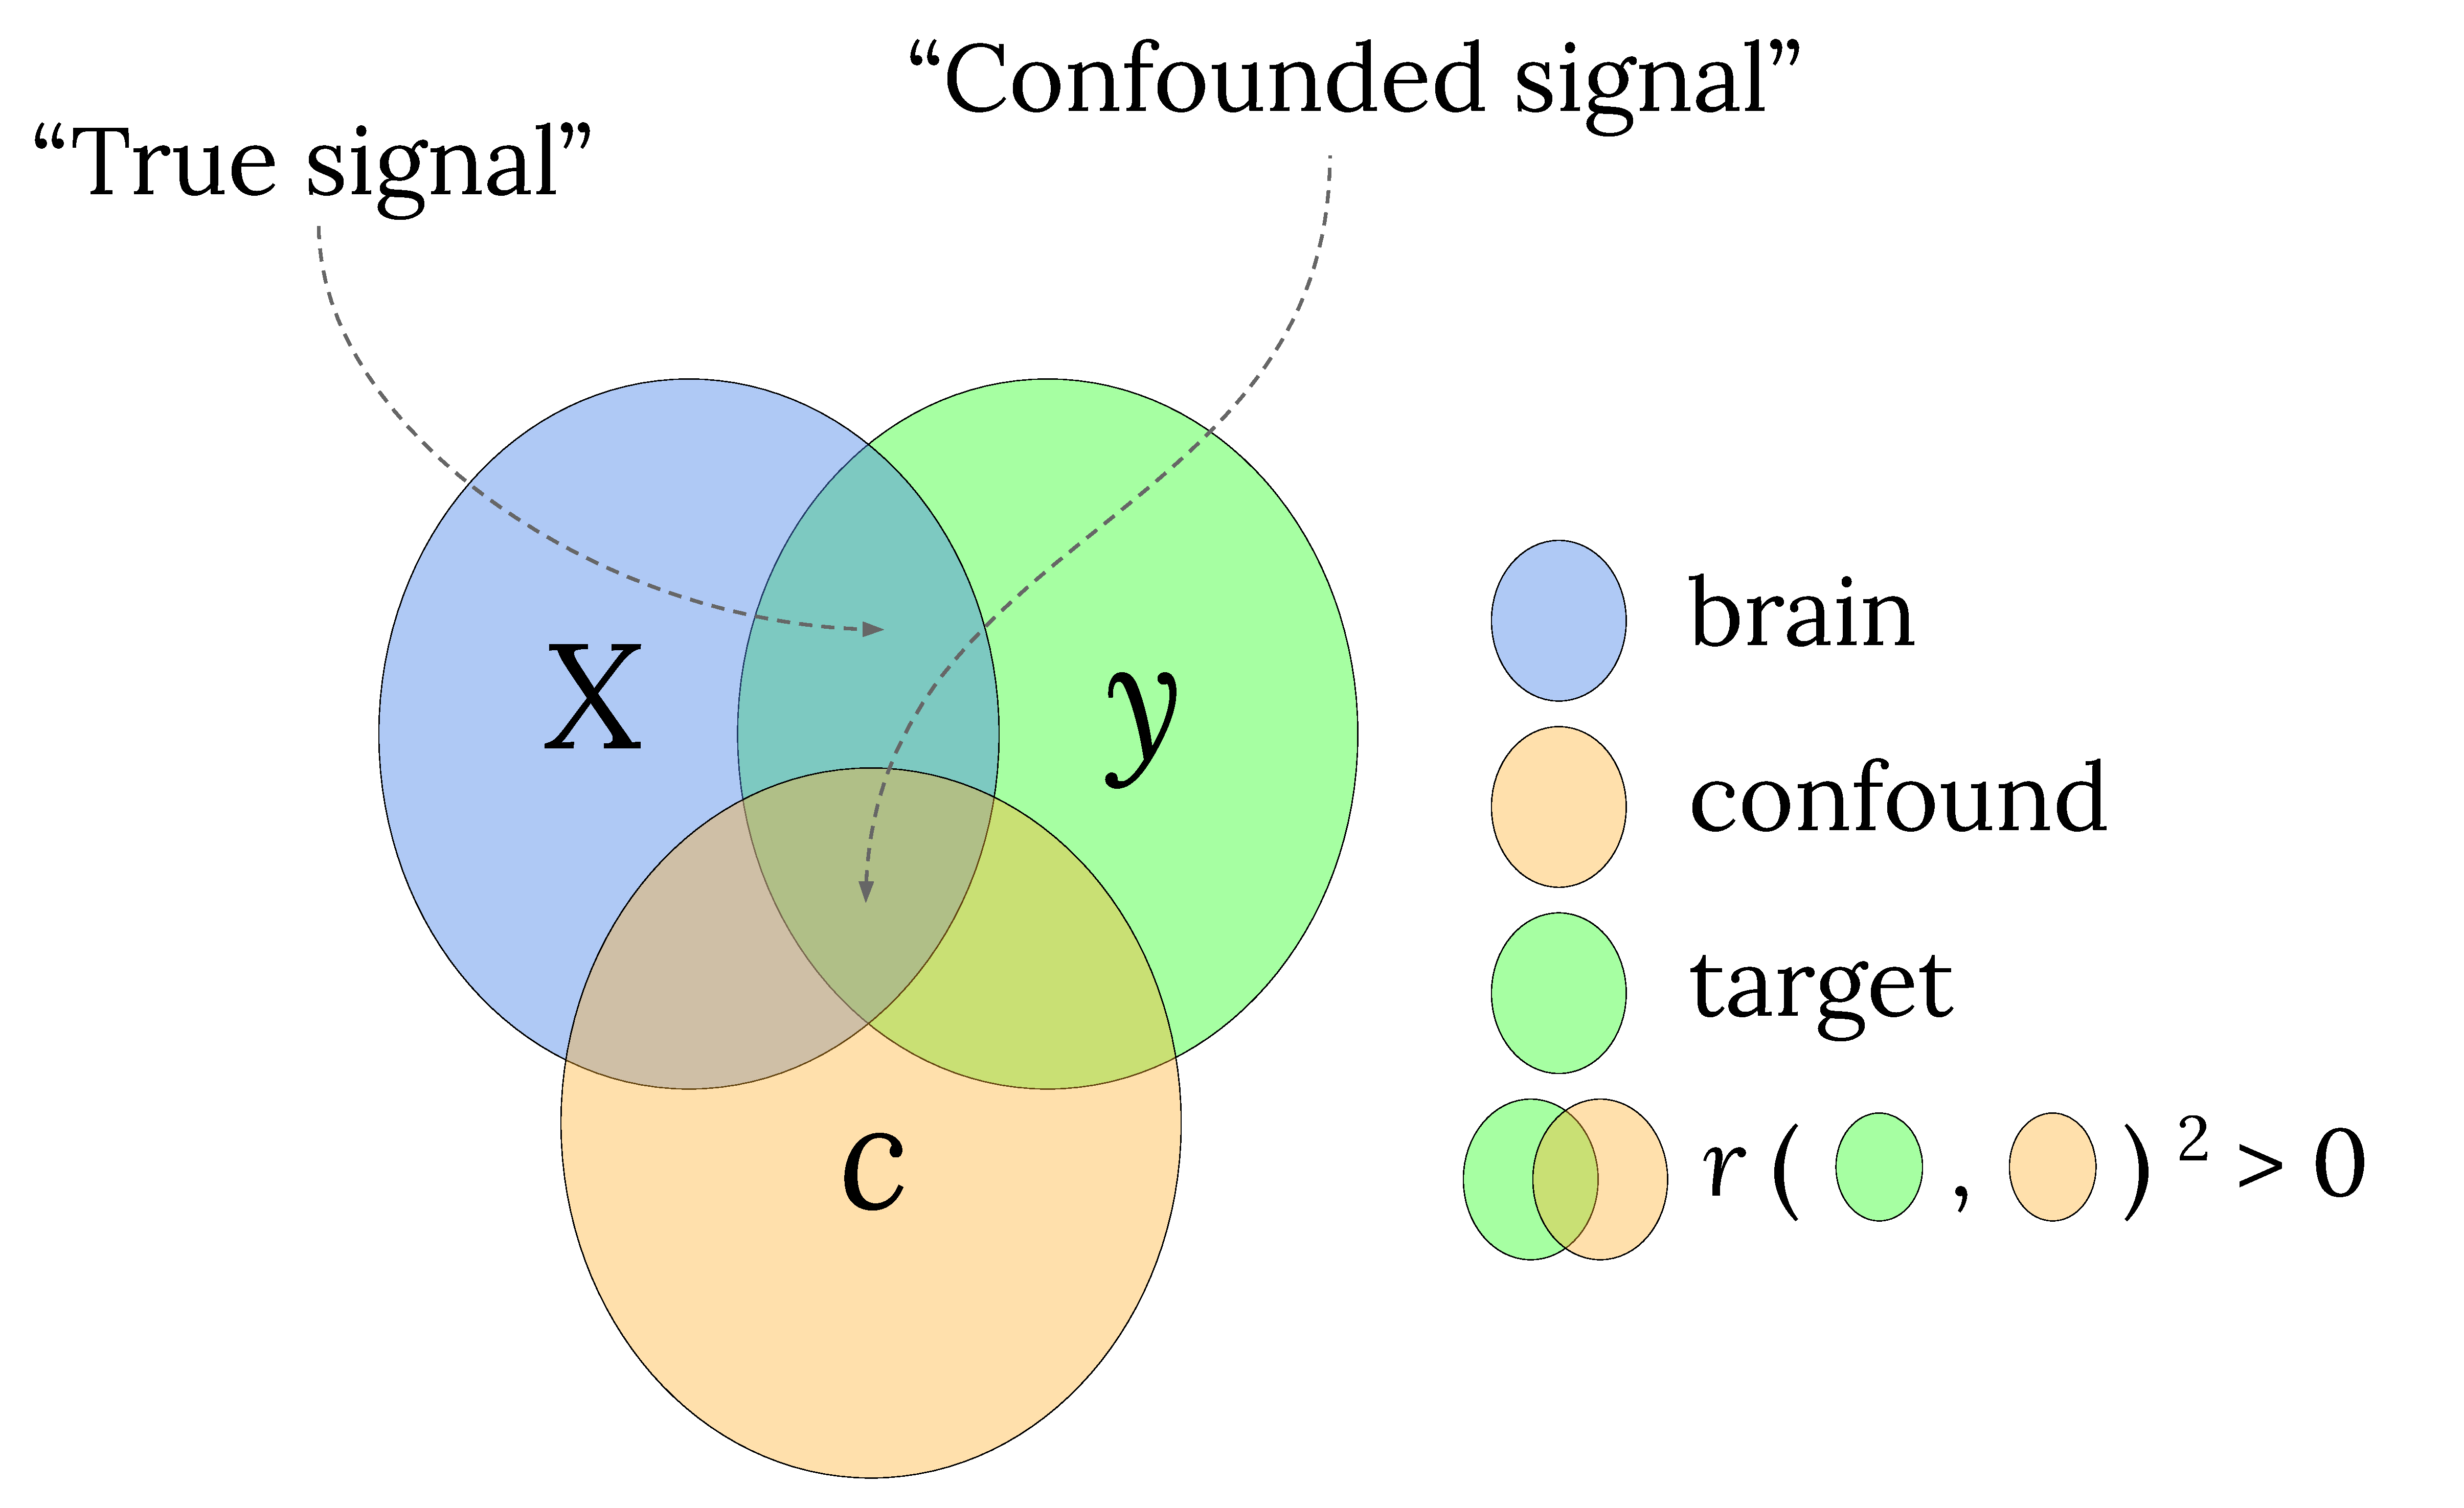
\includegraphics{_bookdown_files/confounds-decoding-files/figures/figure_1.pdf}
\caption{\label{fig:fig-confounds-decoding-1}Visualization of how variance in brain data (\(X\)) can partitioned into ``True signal'' and ``Confounded signal'', depending on the correlation structure between the brain data (\(X\)), the confound (\(C\)), and the target (\(y\)). Overlapping circles indicate a non-zero (squared) correlation between the two variables.}
\end{figure}



In the decoding literature, various methods have been applied to control for confounds. We next provide an overview of these methods, highlight their advantages and disadvantages, and discuss their rationale and the types of research settings they can be applied in. Subsequently, we focus on two of these methods to test whether these methods succeed in controlling for the influence of confounds.

\hypertarget{confounds-decoding-introduction-methods}{%
\subsection{Methods for confound control}\label{confounds-decoding-introduction-methods}}

In decoding analyses, one aims to predict a certain target variable from patterns of neuroimaging data. Various methods discussed in this section are supplemented with a mathematical formalization; for consistency and readability, we define the notation we will use in Table \ref{tab:tab-confounds-decoding-1}.

\begingroup\fontsize{10}{12}\selectfont

\begin{ThreePartTable}
\begin{TableNotes}[para]
\item \textit{Note: } 
\item Format based on Diedrichsen and Kriegeskorte (2017). For the correlations ($r$), we assume that $P = 1$ and thus that the correlations in the table reduce to a scalar.
\end{TableNotes}
\begin{longtabu} to \linewidth {>{\raggedright\arraybackslash}p{3em}>{\raggedright\arraybackslash}p{3em}>{\raggedright}X}
\caption{\label{tab:tab-confounds-decoding-1}Notation.}\\
\toprule
Symbol & Dims. & Description\\
\midrule
$N$ & - & Number of samples (usually subjects or trials)\\
$K$ & - & Number of neuroimaging features (e.g., voxels or sensors)\\
$P$ & - & Number of confound variables (e.g., age, reaction time, or brain size)\\
$X_{ij}$ & $N \times K$ & The neuroimaging patterns (often called the "data" in the current article), where the subescript $i \in {1 \dots N}$ refers to the individual samples (rows), and the subscript $j \in {1 \dots K}$ to individual features (columns)\\
$y$ & $N \times 1$ & The target variable (i.e., what is to be decoded)\\
\addlinespace
$C$ & $N \times P$ & The confound variable(s)\\
$\hat{\beta}$ & $K + 1$ & The parameters estimated in a general linear model (GLM)\\
$w$ & $K + 1$ & The parameters estimated in a decoding model\\
$r_{Cy}$ & - & Sample Pearson correlation coefficient between $C$ and $y$\\
$r_{y(X.C)}$ & - & Sample semipartial Pearson correlation coefficient between $X$ and $y$, controlled for $C$\\
\addlinespace
$p(r_{Cy})$ & - & $p$-value of sample Pearson correlation between $C$ and $y$\\
\bottomrule
\insertTableNotes
\end{longtabu}
\end{ThreePartTable}
\endgroup{}

\hypertarget{confounds-decoding-introduction-methods-apriori-counterbalancing}{%
\subsubsection{A priori counterbalancing}\label{confounds-decoding-introduction-methods-apriori-counterbalancing}}

Ideally, one would prevent confounding variables from influencing the results as much as possible before the acquisition of the neuroimaging data.\footnote{In the context of behavioral data, a priori counterbalancing is often called ``matching'' or a employing a ``case-control design'' (Cook, 2002)} One common way do this (in both traditional ``activation-based'' and decoding analyses) is to make sure that potential confounding variables are \emph{counterbalanced} in the experimental design (Görgen et al., \protect\hyperlink{ref-Gorgen2017-sy}{2017}). In experimental research, this would entail randomly assigning subjects to design cells (e.g., treatment groups) such that there is no structural correlation between characteristics of the subjects and design cells. In observational designs (e.g., in the gender/brain size example described earlier), it means that the sample is chosen such that there is no correlation between the confound (brain size) and \emph{observed} target variable (gender). That is, given that men on average have larger brains than women, this would entail including only men with relatively small brains and women with relatively large brains.\footnote{Note that the counterbalancing process is the same for both traditional univariate (activation-based) studies and decoding studies, but the direction of analysis is reversed in univariate (e.g., gender → brain) and decoding studies (e.g., brain → gender). As such, in univariate studies the confound (e.g., brain size) is counterbalanced with respect to the predictor(s) (e.g., gender) while in decoding studies the confound (e.g., brain size) is counterbalanced with respect to the target (e.g., gender).} The distinction between experimental and observational studies is important because the former allow the researcher to randomly draw samples from the population, while the latter require the researcher to choose a sample that is not representative of the population, which limits the conclusions that can be drawn about the population (we will revisit this issue in the \protect\hyperlink{confounds-decoding-discussion}{Discussion} section).

Formally, in decoding analyses, a design is counterbalanced when the confound \(C\) and the target \(y\) are statistically independent. In practice, this often means that the sample is chosen so that there is no significant correlation coefficient between \(C\) and \(y\) (although this does not necessarily imply that \(C\) and \(y\) are actually independent). To illustrate the process of counterbalancing, let's consider another hypothetical experiment: suppose one wants to set up an fMRI experiment in which the goal is to decode abstract object category (e.g., faces vs.~houses) from the corresponding fMRI patterns (cf.~Haxby et al., \protect\hyperlink{ref-Haxby2001-os}{2001}), while controlling for the potential confounding influence of low-level or mid-level stimulus features, such as luminance, spatial frequency, or texture (Long et al., \protect\hyperlink{ref-Long2017-fb}{2017}). Proper counterbalancing would entail making sure that the images used for this particular experiments have similar values for these low-level and mid-level features across object categories (see for details Görgen et al., \protect\hyperlink{ref-Gorgen2017-sy}{2017}). Thus, in this example, low-level and mid-level stimulus features should be counterbalanced with respect to object category, such that above chance decoding of object category cannot be attributed to differences in low-level or mid-level stimulus features (i.e., the confounds).

A priori counterbalancing of potential confounds is, however, not always feasible. For one, the exact measurement of a potentially confounding variable may be impossible until data acquisition. For example, the brain size of a participant is only known after data collection. Similarly, Todd et al. (\protect\hyperlink{ref-Todd2013-sd}{2013}) found that their decoding analysis of rule representations was confounded by response times of to the to-be-decoded trials. Another example of a ``data-driven'' confound is participant motion during data acquisition (important in, for example, decoding analyses applied to data from clinical populations such as ADHD; Yu-Feng et al., \protect\hyperlink{ref-Yu-Feng2007-sg}{2007}). In addition, a priori counterbalancing of confounds may be challenging because of the limited size of populations of interest. Especially in clinical research settings, researchers may not have the luxury of selecting a counterbalanced sample due to the small number of patient subjects available for testing. Lastly, researchers may simply discover confounds after data acquisition.

Given that a priori counterbalancing is not possible or undesirable in many situations, it is paramount to explore the possibilities of controlling for confounding variables after data acquisition for the sake of model interpretability, which we discuss next.

\hypertarget{confounds-decoding-introduction-methods-include-in-data}{%
\subsubsection{Include confounds in the data}\label{confounds-decoding-introduction-methods-include-in-data}}

One perhaps intuitive method to control for confounds in decoding analyses is to include the confound(s) in the data (i.e., the neuroimaging data, \(X\); see, e.g., Sepehrband et al., \protect\hyperlink{ref-Sepehrband2018-dy}{2018}) used by decoding model. That is, when applying a decoding analysis to neuroimaging data, the confound is added to the data as if it were another voxel (or sensor, in electrophysiology). This intuition may stem from the analogous situation in univariate (activation-based) analyses of neuroimaging data, in which confounding variables are controlled for by including them in the design matrix together with the stimulus/task regressors. For example, in univariate analyses of functional MRI, movement of the participant is often controlled for by including motion estimates in the design matrix of first-level analyses (Johnstone et al., \protect\hyperlink{ref-Johnstone2006-tn}{2006}); in EEG, some control for activity due to eye-movements by including activity measured by concurrent electro-oculography as covariates in the design-matrix (Parra et al., \protect\hyperlink{ref-Parra2005-um}{2005}). Usually, the general linear model is then used to estimate each predictor's influence on the neuroimaging data. Importantly, the parameter estimates (\(\hat{\beta}\)) are often interpreted as reflecting the unique contribution\footnote{However, parameter estimates only reflect unique variance when ordinary, weighted, or generalized least squares is used to find the model parameters. Other (regularized) linear models, such as ridge regression or LASSO, are not guaranteed to yield parameters that explain unique proportions of variance.} of each predictor variable, independent from the influence of the confound.

Contrary to general linear models as employed in univariate (activation-based) analyses, including confound variables in the data as predictors for \emph{decoding} models is arguably problematic. If a confound is included in the data in the context of decoding models, the parameter estimates of the features (often called ``feature weights'', \(w\), in decoding models) may be corrected for the influence of the confound, but the \emph{model performance} (usually measured as explained variance, \(R^2\), or classification accuracy; Hebart \& Baker, \protect\hyperlink{ref-Hebart2017-jn}{2017}) is not. That is, rather than providing an estimate of decoding performance ``controlled for'' a confound, one obtains a measure of performance when explicitly \emph{including} the confound as an interesting source of variance that the decoder is allowed to use. This is problematic because research using decoding analyses generally does not focus on parameter estimates but on statistics of model performance. Model performance statistics (e.g., \(R^2\), classification accuracy) alone cannot disentangle the contribution of different sources of information as they only represent a single summary statistic of model fit (Ritchie et al., \protect\hyperlink{ref-Ritchie2017-gl}{2017}). One might, then, argue that additionally inspecting feature weights of decoding models may help in disambiguating different sources of information (Sepehrband et al., \protect\hyperlink{ref-Sepehrband2018-dy}{2018}). However, it has been shown that feature weights cannot be reliably mapped to specific sources of information, i.e., as being task-related or confound-related (e.g., features with large weights may be completely uncorrelated with the target variable; Haufe et al., \protect\hyperlink{ref-Haufe2014-el}{2014}; Hebart \& Baker, \protect\hyperlink{ref-Hebart2017-jn}{2017}). As such, it does not make sense to include confounds in the set of predictors when the goal is to disambiguate the different sources of information in decoding analyses.

Recently, another approach similar to including confounds in the data has been proposed, which is based on the idea of a dose-response curve (Alizadeh et al., \protect\hyperlink{ref-alizadeh2017decoding}{2017}). In this method, instead of adding the confound(s) to the model directly, the relative contribution of true and confounded signal is systematically controlled. The authors show that this approach is able to directly quantify the unique contribution of each source of information, thus effectively controlling for confounded signal. However, while sophisticated in its approach, this method only seems to work for categorical confounds, as it is difficult (if not impossible) to systematically vary the proportion of confound-related information when dealing with continuous confounds or when dealing with more than one confound.

\hypertarget{confounds-decoding-introduction-methods-pattern-estimation}{%
\subsubsection{Control for confounds during pattern estimation}\label{confounds-decoding-introduction-methods-pattern-estimation}}

Another method that was used in some decoding studies on functional MRI data aims to control for confounds in the initial procedure of estimating activity patterns of the to-be-decoded events, by leveraging the ability of the GLM to yield parameter estimates reflecting unique variance (Woolgar et al., \protect\hyperlink{ref-Woolgar2014-jb}{2014}). In this method, an initial ``first-level'' (univariate) analysis models the fMRI time series (\(s\)) as a function of both predictors-of-interest (\(X\)) and the confounds (\(C\)), often using the GLM\footnote{Note that \(X\) and \(C\), here, refer to (usually HRF-convolved) predictors of the time series signal (\(s\)) for a single voxel. In the rest of the article, \(X\) and \(C\) refer to features that are defined across samples (not time).}:

\begin{equation}
s = X\beta_{x} + C\beta_{c} + \epsilon
\end{equation}

Then, only the estimated parameters (\(\hat{\beta}\), or normalized parameters, such as \emph{t}-values or \emph{z}-values) corresponding to the predictors-of-interest (\(\hat{\beta}_{x}\)) are used as activity estimates (i.e., the used for predicting the target \(y\)) in the subsequent decoding analyses. This method thus takes advantage of the shared variance partitioning in the pattern estimation step to control for potential confounding variables. However, while elegant in principle, this method is not applicable in between-subject decoding studies (e.g., clinical decoding studies; Waarde et al., \protect\hyperlink{ref-Van_Waarde2014-sh}{2014}; Cuingnet et al., \protect\hyperlink{ref-Cuingnet2011-hv}{2011}), in which confounding variables are defined across subjects, or in electrophysiology studies, in which activity patterns do not have to be\footnote{Note that, technically, one could use the ``Control for confounds during pattern estimation'' method in electrophysiology as well, by first fitting a univariate model explaining the neuroimaging data (\(X_{j}\) for \(j = 1 \dots K\)) as a function of both the target (\(y\)) and the confound (\(C\)) and subsequently only using the parameter estimates of the target-predictor (\(\hat{\beta}_{x}\)) as patterns in the subsequent decoding analysis.} estimated in a first-level model, thus limiting the applicability of this method.

\hypertarget{confounds-decoding-introduction-methods-posthoc-counterbalancing}{%
\subsubsection{Post hoc counterbalancing of confounds}\label{confounds-decoding-introduction-methods-posthoc-counterbalancing}}

When a priori counterbalancing is not possible, some have argued that post hoc counterbalancing might control for the influence of confounds (Rao et al., \protect\hyperlink{ref-Rao2017-bw}{2017}, pp. 24, 38). In this method, given that there is some sample correlation between the target and confound (\(r_{Cy} \neq 0\)) in the entire dataset, one takes a subset of samples in which there is no empirical relation between the confound and the target (e.g., when \(r_{Cy} \approx 0\)). In other words, post hoc counterbalancing is a way to \emph{decorrelate} the confound and the target by subsampling the data. Then, subsequent decoding analysis on the subsampled data can only capitalize on true signal, as there is no confounded signal anymore (see Figure \ref{fig:fig-confounds-decoding-2}). While intuitive in principle, we are not aware of whether this method has been evaluated before and whether it yields unbiased performance estimates.

\begin{figure}
\centering
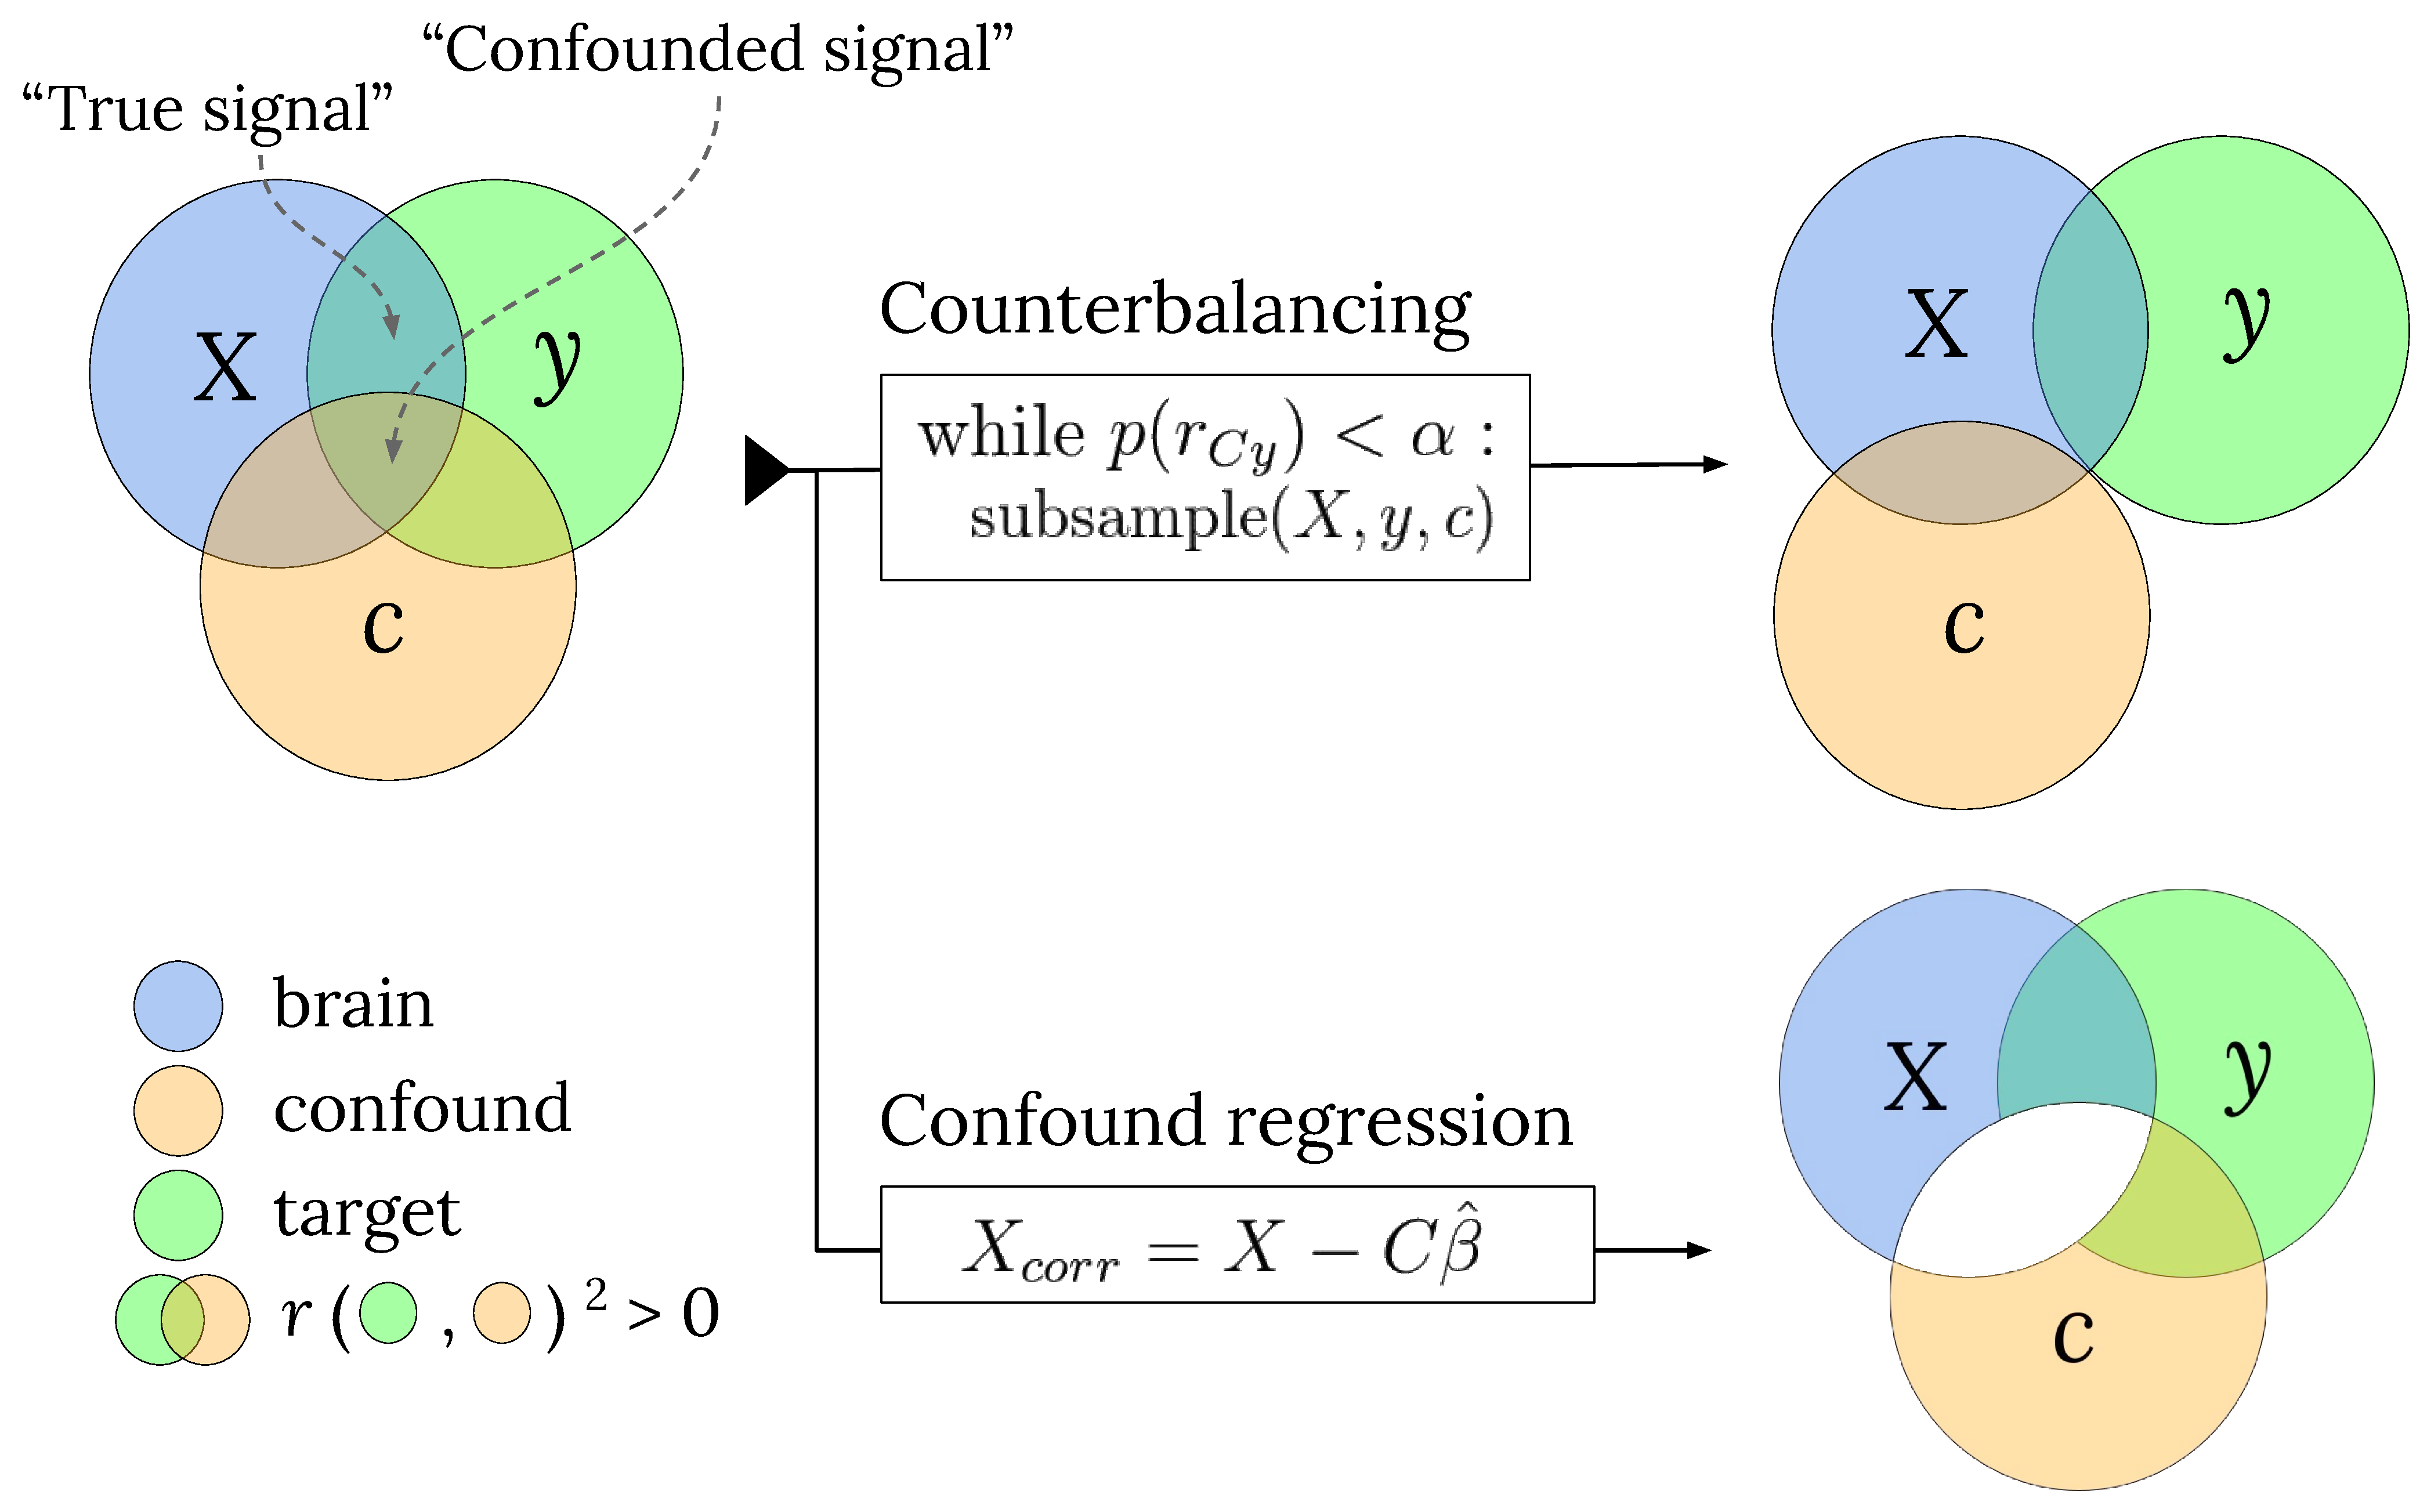
\includegraphics{_bookdown_files/confounds-decoding-files/figures/figure_2.pdf}
\caption{\label{fig:fig-confounds-decoding-2}A schematic visualization how the main two confound control methods evaluated in this article deal with the ``confounded signal'', making sure decoding models only capitalize on the ``true signal''.}
\end{figure}



\hypertarget{confounds-decoding-introduction-methods-confound-regression}{%
\subsubsection{Confound regression}\label{confounds-decoding-introduction-methods-confound-regression}}

The last and perhaps most common method to control for confounds is removing the variance that can be explained by the confound (i.e., the confounded signal) from the neuroimaging data directly (Abdulkadir et al., \protect\hyperlink{ref-Abdulkadir2014-bh}{2014}; Dukart et al., \protect\hyperlink{ref-Dukart2011-aq}{2011}; Kostro et al., \protect\hyperlink{ref-Kostro2014-cm}{2014}; Rao et al., \protect\hyperlink{ref-Rao2017-bw}{2017}; Todd et al., \protect\hyperlink{ref-Todd2013-sd}{2013}) --- a process we refer to as \emph{confound regression} (also known as ``image correction''; Rao et al., \protect\hyperlink{ref-Rao2017-bw}{2017}). In this method, a (usually linear) regression model is fitted on each feature in the neuroimaging data (i.e., a single voxel or sensor) with the confound(s) as predictor(s). Thus, each feature in the neuroimaging data \(X\) is modelled as a linear function of the confounding variable(s), \(C\):

\begin{equation}
X_{j} = C\beta + \epsilon
\end{equation}

We can estimate the parameter(s) for feature using, for example, ordinary least squares as follows (for an example using a different model, see Abdulkadir et al., \protect\hyperlink{ref-Abdulkadir2014-bh}{2014}):

\begin{equation}
\hat{\beta}_{j} = (C^{T}C)^{-1}C^{T}X_{j}
\end{equation}

Then, to remove the variance of (or ``regress out'') the confound from the neuroimaging data, we can subtract the variance in the data associated with confound (\(C\hat{\beta}_{j}\)) from the original data:

\begin{equation}
X_{j,\mathrm{corr}} = X_{j} - C\hat{\beta}_{j}
\end{equation}

In which \(X_{j,\mathrm{corr}}\) represents the neuroimaging feature \(X_{j}\) from which all variance of the confound is removed (including the variance shared with \(y\), i.e., the confounded signal; see Figure \ref{fig:fig-confounds-decoding-2}). When subsequently applying a decoding analysis on this corrected data, one can be sure that the decoder is not capitalizing on signal that is correlated with the confound, which thus improves interpretability of the decoding analysis.

Confound regression has been applied in several decoding studies. Todd et al. (\protect\hyperlink{ref-Todd2013-sd}{2013}) were, as far as the current authors are aware, the first to use this method to control for a confound (in their case, reaction time) that was shown to correlate with their target variable (rule A vs.~rule B). Notably, they both regressed out reaction time from the first-level time series data (similar to the ``Control for confounds during pattern estimation'' method) \emph{and} regressed out reaction time from the trial-by-trial activity estimates (i.e., confound regression as described in this section). They showed that controlling for reaction time in this way completely eliminated the above chance decoding performance. Similarly, Kostro et al. (\protect\hyperlink{ref-Kostro2014-cm}{2014}) observe a substantial drop in classification accuracy when controlling for scanner site in the decoding analysis of Huntington's disease, but only when scanner site and disease status were actually correlated. Lastly, Rao et al. (\protect\hyperlink{ref-Rao2017-bw}{2017}) found that, in contrast to Kostro et al.~and Todd et al., confound regression yielded similar (or slightly lower, but still significant) performance compared to the model without confound control, but it should be noted that this study used a regression model (instead of a classification model) and evaluated confound control in the specific situation when the training set is confounded, but the test set is not.\footnote{Note that we did not discuss studies that implement a different confound regression procedure (e.g., Abdulkadir et al., \protect\hyperlink{ref-Abdulkadir2014-bh}{2014}; Dukart et al., \protect\hyperlink{ref-Dukart2011-aq}{2011}), in which confound regression is only estimated on the samples from a single class of the target variable (e.g., in our gender decoding example, this would mean that confound regression models are only estimated on the data from male, or female, subjects). As this form of confound regression does not disambiguate the sources of information driving the decoder, it is not discussed further in this article.} In sum, while confound regression has been used before, it has yielded variable results, possibly due to slightly different approaches and differences in the correlation between the confounding variable and the target.

\hypertarget{confounds-decoding-introduction-current-study}{%
\subsection{Current study}\label{confounds-decoding-introduction-current-study}}

In summary, multiple methods have been proposed to deal with confounds in decoding analyses. Often, these methods have specific assumptions about the nature or format of the data (such as ``A priori counterbalancing'' and ``Confound control during pattern estimation''), differ in their objective (e.g., \emph{prediction} vs.~\emph{interpretation}, such as in ``Include confounds in the data''), or have yielded variable results (such as ``Confound regression''). Therefore, given that we are specifically interested in interpreting decoding analyses, the current study evaluates the two methods that are applicable in most contexts: post hoc counterbalancing and confound regression (but see \protect\hyperlink{confounds-decoding-supplement}{Supplementary Materials} for a tentative evaluation of this method based on simulated functional MRI data). In addition to these two methods, we propose a third method --- a modified version of confound regression ----- which we show yields plausible, seemingly unbiased, and interpretable results.

To test whether these methods are able to effectively control for confounds and whether they yield plausible results, we apply them to empirical data, as well as to simulated data in which the ground truth with respect to the signal in the data (i.e., the proportion of true signal and confounded signal) is known. For our empirical data, we enact the previously mentioned hypothetical study in which participant gender is decoded from structural MRI data. We use a large dataset (\(N = 217\)) of structural MRI data and try to predict subjects' gender (male/female) from gray and white matter patterns while controlling for the confound of ``brain size'' using the aforementioned methods, which we compare to a baseline model in which confounds are not controlled for. Given the previously reported high correlations between brain size and gender (Barnes et al., \protect\hyperlink{ref-Barnes2010-pu}{2010}; Smith \& Nichols, \protect\hyperlink{ref-Smith2018-th}{2018}), we expect that successfully controlling for brain size yields lower decoding performance than using uncorrected data, but not below chance level. Note that higher decoding performance after controlling for confounds is theoretically possible when the correlation between the confound and variance in the data \emph{unrelated} to the target (e.g., noise) is sufficiently high to cause suppressor effects (see Figure 1 in Haufe et al., \protect\hyperlink{ref-Haufe2014-el}{2014}; Hebart \& Baker, \protect\hyperlink{ref-Hebart2017-jn}{2017}). However, because our confound, brain size, is known to correlate strongly with our target gender (approx. \(r = 0.63\); Smith \& Nichols, \protect\hyperlink{ref-Smith2018-th}{2018}), it is improbable that it also correlates highly with variance in brain data that is unrelated to gender. It follows then that classical suppression effects are unlikely and we thus expect lower model performance after controlling for brain size.

However, shown in detail below, both post hoc counterbalancing and confound regression lead to unexpected results in our empirical analyses: counterbalancing fails to reduce model performance while confound regression consistently yields low model performance up to the point of significant below chance accuracy. In subsequent analyses of simulated data, we show that both methods lead to \emph{biased} results: post hoc counterbalancing yields inflated model performance (i.e., positive bias) because subsampling selectively selects a subset of samples in which features correlate more strongly with the target variable, suggesting (indirect) circularity in the analysis (Kriegeskorte et al., \protect\hyperlink{ref-kriegeskorte2009circular}{2009}). Furthermore, our simulations show that negative bias (including significant below chance classification) after confound regression on the entire dataset is due to reducing the signal below what is expected by chance (Jamalabadi et al., \protect\hyperlink{ref-Jamalabadi2016-gr}{2016}), which we show is related to and can be predicted by the standard deviation of the empirical distribution of correlations between the features in the data and the target. We propose a minor but crucial addition to the confound regression procedure, in which we cross-validate the confound regression models (which we call ``cross-validated confound regression'', CVCR), which solves the below chance accuracy issue and yields plausible model performance in both our empirical and simulated data.

\hypertarget{confounds-decoding-methods}{%
\section{Methods}\label{confounds-decoding-methods}}

\hypertarget{confounds-decoding-methods-data}{%
\subsection{Data}\label{confounds-decoding-methods-data}}

For the empirical analyses, we used voxel-based morphometry (VBM) data based on T1-weighted scans and tract-based spatial statistics (TBSS) data based on diffusion tensor images from 217 participants (122 women, 95 men), acquired with a Philips Achieva 3T MRI-scanner and a 32-channel head coil at the Spinoza Centre for Neuroimaging (Amsterdam, The Netherlands).

\hypertarget{confounds-decoding-methods-data-vbm}{%
\subsubsection{VBM acquisition \& analysis}\label{confounds-decoding-methods-data-vbm}}

The T1-weighted scans with a voxel size of 1.0 × 1.0 × 1.0 mm were acquired using 3D fast field echo (TR: 8.1 ms, TE: 3.7 ms, flip angle: 8°, FOV: 240 × 188 mm, 220 slices). We used ``FSL-VBM'' protocol (Douaud et al., \protect\hyperlink{ref-Douaud2007-sw}{2007}) from the FSL software package (version 5.0.9; Smith et al., \protect\hyperlink{ref-Smith2004-sc}{2004}); using default and recommended parameters (including non-linear registration to standard space). The resulting VBM-maps were spatially smoothed using a Gaussian kernel (3 mm FWHM). Subsequently, we organized the data in the standard pattern-analysis format of a 2D (\(N \times K\)) array of shape 217 (subjects) × 412473 (non-zero voxels).

\hypertarget{confounds-decoding-methods-data-tbss}{%
\subsubsection{TBSS acquisition \& analysis}\label{confounds-decoding-methods-data-tbss}}

Diffusion tensor images with a voxel size of 2.0 × 2.0 × 2.0 mm were acquired using a spin-echo echo-planar imaging (SE-EPI) protocol (TR: 7476 ms, TE: 86 ms, flip angle: 90°, FOV: 224 × 224 mm, 60 slices), which acquired a single b = 0 (non-diffusion-weighted) image and 32 (diffusion-weighted) b = 1000 images. All volumes were corrected for eddy-currents and motion (using the FSL command ``eddy\_correct'') and the non-diffusion-weighted image was skullstripped (using FSL-BET with the fractional intensity threshold set to 0.3) to create a mask that was subsequently used in the fractional anisotropy (FA) estimation. The FA-images resulting from the diffusion tensor fitting procedure were subsequently processed by FSL's tract-based spatial statistics (TBSS) pipeline (Smith et al., \protect\hyperlink{ref-Smith2006-sf}{2006}), using the recommended parameters (i.e., non-linear registration to FSL's 1 mm FA image, construction of mean FA-image and skeletonized mean FA-image based on the data from all subjects, and a threshold of 0.2 for the skeletonized FA-mask). Subsequently, we organized the resulting skeletonized FA-maps into a 2D (\(N \times K\)) array of shape 217 (subjects) × 128340 (non-zero voxels).

\hypertarget{confounds-decoding-methods-data-brainsize}{%
\subsubsection{Brain size estimation}\label{confounds-decoding-methods-data-brainsize}}

To estimate the values for our confound, global brain size, we calculated for each subject the total number of non-zero voxels in the gray matter and white matter map resulting from the segmentation step in the FSL-VBM pipeline (using FSL's segmentation algorithm ``FAST''; Zhang et al., \protect\hyperlink{ref-Zhang2001-wa}{2001}). The number of non-zero voxels from the gray matter map was used as the confound for the VBM-based analyses and the number of non-zero voxels from the white matter map was used as the confound for the TBSS-based analyses. Note that brain size estimates from total white matter volume and total gray matter volume correlated strongly, \(r (216) = 0.93\), \(p < 0.001\).

\hypertarget{confounds-decoding-methods-data-data-and-code}{%
\subsubsection{Data and code availability}\label{confounds-decoding-methods-data-data-and-code}}

In the Github repository corresponding to this article (\url{https://github.com/lukassnoek/MVCA}), we included a script (\texttt{download\_data.py}) to download the data (the 4D VBM and TBSS nifti-images as well as the non-zero 2D samples × features arrays). The repository also contains detailed Jupyter notebooks with the annotated empirical analyses and simulations reported in this article.

\hypertarget{confounds-decoding-methods-pipeline}{%
\subsection{Decoding pipeline}\label{confounds-decoding-methods-pipeline}}

All empirical analyses and simulations used a common decoding pipeline, implemented using functionality from the \emph{scikit-learn} Python package for machine learning (Abraham et al., \protect\hyperlink{ref-Abraham2014-ef}{2014}; Pedregosa et al., \protect\hyperlink{ref-pedregosa2011scikit}{2011}). This pipeline included univariate feature selection (based on a prespecified amount of voxels with highest univariate difference in terms of the ANOVA \emph{F}-statistic), feature-scaling (ensuring zero mean and unit standard deviation for each feature), and a support vector classifier (SVC) with a linear kernel, fixed regularization parameter (\emph{C} = 1), and sample weights set to be inversely proportional to class frequency (to account for class imbalance). In our empirical analyses, we evaluated model performance for different numbers of voxels (as selected by the univariate feature selection). For our empirical analyses, we report model performance as the \(F_{1}\) score, which is insensitive to class imbalance (which, in addition to adjusted sample weights, prevents the classifier from learning the relative probabilities of target classes instead of representative information in the features; see also Supplementary Figure \ref{fig:fig-confounds-decoding-S14} for a replication of part of the results using AUROC, another metric that is insensitive to class imbalance). At chance level classification, the \(F_{1}\) score is expected to be 0.5. For our simulations, in which there is no class imbalance, we report model performance using accuracy scores. In figures showing error bars around the average model performance scores, the error bars represent 95\% confidence intervals estimated using the ``bias-corrected and accelerated'' (BCA) bootstrap method using 10,000 bootstrap replications (Efron, \protect\hyperlink{ref-efron1987better}{1987}). For calculating BCA bootstrap confidence intervals, we used the implementation from the open source ``scikits.bootstrap'' Python package (\url{https://github.com/cgevans/scikits-bootstrap}). Statistical significance was calculated using non-parametric permutation tests, as implemented in scikit-learn, with 1000 permutations (Ojala \& Garriga, \protect\hyperlink{ref-Ojala2010-rc}{2010}).

\hypertarget{confounds-decoding-methods-evaluated-methods}{%
\subsection{Evaluated methods for confound control}\label{confounds-decoding-methods-evaluated-methods}}

\hypertarget{confounds-decoding-methods-evaluated-methods-counterbalancing}{%
\subsubsection{Post hoc counterbalancing}\label{confounds-decoding-methods-evaluated-methods-counterbalancing}}

We implemented post hoc counterbalancing in two steps. First, to quantify the strength of relation between the confound and the target in our dataset, we estimated the point-biserial correlation coefficient between the confound, \(C\) (brain size), and the target, \(y\) (gender) across the entire dataset (including all samples \(i = 1 \dots N\)). Because of both sampling noise and measurement noise, sample correlation coefficients vary around the population correlation coefficient and are thus improbable to be 0 \emph{exactly}.\footnote{For continuous confounds, it is practically impossible to achieve a correlation with the target of \emph{exactly} zero, which is the reason we subsample until it is smaller than a prespecified threshold. For categorical confounds, however, a correlation between the confound and the target of exactly zero is possible (this amounts to equal proportions of levels of \(c\) within each class of \(y\); Görgen et al., \protect\hyperlink{ref-Gorgen2017-sy}{2017}), even \emph{necessary}, because it is impossible to find a (\emph{K}-fold) cross-validation partitioning in which each split is counterbalanced w.r.t. the confound if the correlation \emph{in the entire dataset} between the target and the confound is not zero.} Therefore, in the next step, we subsampled the data until the correlation coefficient between and becomes non-significant at some significance threshold \(\alpha\): \(p(r_{Cy}) > \alpha\).

In our analyses, we used an \(\alpha\) of 0.1. Note that this is more ``strict''\footnote{We refer to a relatively high α as ``strict'', here, because we use it here for the purpose of demonstrating no effect.} than the conventionally used threshold (\(\alpha = 0.05\)), but given that decoding analyses are often more sensitive to signal in the data (whether it is confounded or true signal), we chose to err on the safe side and counterbalance the data using a relatively strict threshold of \(\alpha = 0.1\).

Subsampling was done by iteratively removing samples that contribute most to the correlation between the confound and the target until the correlation becomes non-significant. In our empirical data in which brain size is positively correlated with gender (coded as male = 1, female = 0) this amounted to iteratively removing the male subject with the largest brain size and the female subject with the smallest brain size. This procedure optimally balances (1) minimizing the correlation between target and confound and (2) maximizing sample size. As an alternative to this ``targeted subsampling'', we additionally implemented a procedure which draws random subsamples of a given sample size until it finds a subsample with a non-significant correlation coefficient. If such a subsample cannot be found after 10,000 random draws, sample size is decreased by 1, which is repeated until a subsample is found. This procedure resulted in much smaller subsamples than the targeted subsampling procedure (i.e., a larger power loss) since the optimal subsample is hard to find randomly.\footnote{One could run the ``random subsampling'' procedure with more than 10,000 draws in order to reduce the aforementioned power loss; but in the extreme, this would result in the same optimal subsample that can be found much faster by targeted subsampling.} In the analyses below, therefore, we used the targeted subsampling procedure. Importantly, even with extreme power loss, random subsampling can cause the same biases as will be described for the targeted subsampling method below (cf.~Figure \ref{fig:fig-confounds-decoding-8} and Figure \ref{fig:fig-confounds-decoding-10} and Supplementary Figures \ref{fig:fig-confounds-decoding-S13} and \ref{fig:fig-confounds-decoding-S14}).

Then, given that the subsampled dataset is counterbalanced with respect to the confound, a random stratified K-fold cross-validation scheme is repeatedly initialized until a scheme is found in which \emph{all} splits are counterbalanced as well (cf.~Görgen et al., \protect\hyperlink{ref-Gorgen2017-sy}{2017}). This particular counterbalanced cross-validation scheme is subsequently used to cross-validate the MVPA pipeline. We implemented this post hoc counterbalancing method as a scikit-learn-style cross-validator class, available from the aforementioned Github repository (in the \texttt{counterbalance.py} module).

\hypertarget{confound-regression}{%
\subsubsection{Confound regression}\label{confound-regression}}

In our empirical analyses and simulations, we tested two different versions of confound regression, which we call ``whole-dataset confound regression'' (WDCR) and ``cross-validated confound regression'' (CVCR). In WDCR, we regressed out the confounds from the predictors \emph{from the entire dataset at once}, i.e., before entering the iterative cross-validated MVPA pipeline (the approach taken by Abdulkadir et al., \protect\hyperlink{ref-Abdulkadir2014-bh}{2014}; Dubois et al., \protect\hyperlink{ref-dubois2018resting}{2018}; Kostro et al., \protect\hyperlink{ref-Kostro2014-cm}{2014}; Todd et al., \protect\hyperlink{ref-Todd2013-sd}{2013}). Note that we can do this for all \(K\) voxels at once using the closed-form OLS solution, in which we first estimated the parameters \(\hat{\beta}_{C}\):

\begin{equation}
\hat{\beta}_{C} = (C^{T}C)^{-1}C^{T}X
\end{equation}

where \(C\) is an array in which the first column contained an intercept and the second column contained the confound brain size. Accordingly, \(\hat{\beta}_{C}\) is an \(2 \times K\) array. We then removed the variance associated with the confound from our neuroimaging data as follows:

\begin{equation}
X_{\mathrm{corr}} = X - C\hat{\beta}_{C}
\end{equation}

Now, \(X_{\mathrm{corr}}\) is an array with the same shape as the original \(X\) array, but without any variance that can be explained by confound, \(C\) (i.e., \(X\) is residualized with regard to \(C\)).

In our proposed cross-validated version of confound regression (which was mentioned but not evaluated by Rao et al., \protect\hyperlink{ref-Rao2017-bw}{2017}, p. 25), ``CVCR'', we similarly regressed out the confounds from the neuroimaging data, but instead of estimating \(\hat{\beta}_{C}\) on the entire dataset, we estimated this within each fold of training data (\(X_{\mathrm{train}}\)):

\begin{equation}
\hat{\beta}_{C,\mathrm{train}} = (C^{T}_{\mathrm{train}}C_{\mathrm{train}})^{-1}C^{T}_{\mathrm{train}}X_{\mathrm{train}}
\end{equation}

And we subsequently used these parameters (\(\hat{\beta}_{C,\mathrm{train}}\)) to remove the variance related to the confound from both the train set (\(X_{\mathrm{train}}\) and \(C_{\mathrm{train}}\)):

\begin{equation}
X_{\mathrm{train, corr}} = X_{\mathrm{train}} - C_{\mathrm{train}}\hat{\beta}_{C,\mathrm{train}}
\label{eq:cvcr-train}
\end{equation}

and the test test (\(X_{\mathrm{test}}\) and \(C_{\mathrm{test}}\)):

\begin{equation}
X_{\mathrm{test, corr}} = X_{\mathrm{test}} - C_{\mathrm{test}}\hat{\beta}_{C,\mathrm{test}}
\label{eq:cvcr-test}
\end{equation}

Thus, essentially, CVCR is the cross-validated version of WDCR. One might argue that regressing the confound from the train set only, i.e., implementing only equation \eqref{eq:cvcr-train}, not equation \eqref{eq:cvcr-test}, is sufficient to control for confounds as it prevents the decoding model from relying on signal related to the confound. We evaluated this method and report the corresponding results in Supplementary Figure \ref{fig:fig-confounds-decoding-S10}.

We implemented these confound regression techniques as a \emph{scikit-learn} compatible transformer class, available in the open-source \emph{skbold} Python package (\url{https://github.com/lukassnoek/skbold}) and in the aforementioned Github repository.

\hypertarget{control-for-confounds-during-pattern-estimation}{%
\subsubsection{Control for confounds during pattern estimation}\label{control-for-confounds-during-pattern-estimation}}

In addition to post hoc counterbalancing and confound regression, we also evaluated how well the ``control for confounds during pattern estimation'' method controls for the influence of confounds in decoding analyses of (simulated) fMRI data. The simulation methods and results can be found in the \protect\hyperlink{confounds-decoding-supplement}{Supplementary Materials}.

\hypertarget{analyses-of-simulated-data}{%
\subsection{Analyses of simulated data}\label{analyses-of-simulated-data}}

In addition to the empirical evaluation of counterbalancing and confound regression in the gender decoding example, we ran three additional analyses on simulated data. First, we investigated the efficacy of the three confound control methods on synthetic data with known quantities of ``true signal'' and ``confounded signal'', in order to detect potential biases. Second, we ran additional analyses on simulated data to investigate the positive bias in model performance observed after post hoc counterbalancing. Third, we ran additional analyses on simulated data to investigate the negative bias in model performance observed after WDCR. In the \protect\hyperlink{confounds-decoding-supplement}{Supplementary Materials}, we investigate whether the confound regression results generalize to (simulated) functional MRI data (Supplementary Figure \ref{fig:fig-confounds-decoding-S1} and \ref{fig:fig-confounds-decoding-S2}).

\hypertarget{efficacy-analyses}{%
\subsubsection{Efficacy analyses}\label{efficacy-analyses}}

In this simulation, we evaluated the efficacy of the three methods for confound control on synthetic data with a prespecified correlation between the confound and the target, \(r_{Cy}\), and varying amounts of ``confounded signal'' (i.e., the explained variance in \(y\) driven by shared variance between \(X\) and \(y\)). These simulations allowed us to have full control over (and knowledge of) the influence of both signal and confound in the data, and thereby help us diagnose biases associated with post hoc counterbalancing and confound regression.

Specifically, in this efficacy analysis, we generated hypothetical data sets holding the correlation coefficient between \(C\) and \(y\) constant, while varying the amount of true signal and confounded signal. We operationalized true signal as the squared semipartial Pearson correlation between \(y\) and each feature in \(X\), controlled for \(C\). As such, we will refer to this term as \(\mathrm{signal}\ R^{2}\):

\begin{equation}
\mathrm{signal}\ R^{2} = r_{y(X.C)}^{2}
\end{equation}

In the simulations reported and shown in the main article, we used \(r_{Cy} = 0.65\), which corresponds to the observed correlation between brain size and gender in our dataset. To generate synthetic data with this prespecified structure, we generated (1) a data matrix \(X\) of shape \(N\times K\), (2) a target variable \(y\) of shape \(N \times 1\), and (3) a confound variable \(C\) of shape \(N \times P\). For all simulations, we used the following parameters: \(N = 200\), \(K = 5\), and \(P = 1\) (i.e., a single confound variable). We generated \(y\) as a categorical variable with binary values, \(y \in \{0, 1\}\), with equal class probabilities (i.e., 50\%), given that most decoding studies focus on binary classification. We generated \(C\) as a continuous random variable drawn from a standard normal distribution. We generated each feature \(X_{j}\) as a linear combination of \(y\) and \(C\) plus Gaussian noise. Thus, for each predictor \(j = 1 \dots K\) in \(X_{j}\):

\begin{equation}
X_{j} = \beta_{y}y + \beta_{C}C + \epsilon, \epsilon \sim \mathcal{N}(0, \gamma)
\end{equation}

in which \(\beta_{y}\) represented the weight given to \(y\), and \(\beta_{C}\) represented the weight given to \(C\) in the generation of the feature \(X_{j}\), and \(\mathcal{N}(0, \gamma)\) is the normal distribution with zero mean and standard deviation \(\gamma\). The parameters \(\beta_{y}\) and \(\beta_{C}\) were both initialized with a value of 1. First, if the difference between the total variance explained and the sum of the desired signal \(R^2\) and confound \(R^2\) values was larger than 0.01, the standard deviation of the normal distribution from which the errors were drawn (i.e., \(\gamma\)) was adjusted (decreased with 0.01 when the total \(R^2\) is too low, increased with 0.01 when the total \(R^2\) is too high), after which was generated again. This process was iterated until the target total \(R^2\) value is found. Then, the total variance explained was partitioned into confound \(R^2\) and signal \(R^2\). If one or both of these values differed from the targeted values by more than 0.01, the generative parameters \(\beta_{y}\) and \(\beta_{C}\) were adjusted: if signal \(R^2\) is too low, was increased with 0.01, and decreased with 0.01 otherwise. If confound \(R^2\) is too low, \(\beta_{C}\) was increased with 0.01, and decreased with 0.01 otherwise. After adjusting these parameters, \(X_{j}\) was generated again. This process was iterated until the data contain the desired ``true signal'' and ``confounded signal''.

We evaluated the different methods for confound control for two values of signal \(R^2\) (0.004, representing plausible null data,\footnote{Note that plausible null data do not reflect a signal \(R^2\) of 0, because this statistic is biased towards values larger than 0 (because it represents a squared number) when dealing with noisy data, hence our choice of signal \(R^2 = 0.004\).} and 0.1, representing a plausible true effect) and a range of confound \(R^2\) values (in steps of 0.05: \(0.00, 0.05, 0.10, \dots , 0.35\)). This simulation was iterated 10 times (with different partitions of the folds) to ensure the results were not influenced by random noise. Importantly, the specific scenario in which confound \(R^2\) equals 0, which represents data without any confounded signal (\(r_{yX}^2\)), served as ``reference model performance'' to which we can compare the efficacy the confound control methods. This comparison allowed us to detect potential biases.

After the data were generated, a baseline model (no confound control) and the three methods outlined above (post hoc counterbalancing, WDCR, and CVCR) were applied to the simulated data using the standard pipeline described in the \protect\hyperlink{confounds-decoding-methods-pipeline}{Decoding pipeline} section (but without univariate feature selection) and compared to the reference performance.

\hypertarget{confounds-decoding-methods-counterbalancing-bias}{%
\subsubsection{Analysis of positive bias after post hoc counterbalancing}\label{confounds-decoding-methods-counterbalancing-bias}}

As detailed below, post hoc counterbalancing did not lead to the expected decrease in model performance; instead, there appeared to be a trend towards an \emph{increase} in model performance. To further investigate the cause of this unexpected result, we simulated a multivariate normal dataset with three variables, reflecting our data (\(X\)), target (\(y\)), and confound (\(C\)), with 1000 samples (\(N\)) and a single feature (\(K = 1\)). We iterated this data generation process 1000 times and subsequently selected the dataset which yielded the largest (positive) difference between model performance after post hoc counterbalancing versus no confound control. In other words, we used the dataset in which the counterbalancing issue was most apparent. While not necessarily representative of typical (neuroimaging) datasets, this process allowed us to explain and visualize how it is possible that model performance increases after counterbalancing the data.

To generate data from a multivariate normal distribution, we first generated variance-covariance matrices with unit variance for all variables, so that covariances can be interpreted as correlations. The covariances in the matrix were generated as pairwise correlations (\(r_{yX}\), \(r_{Cy}\), \({r_CX}\)), each sampled from a uniform distribution with range \([-0.65, 0.65]\). We generated data using such prespecified correlation structure because the relative increase in model performance after counterbalancing did not appear to occur when generating completely random (normally distributed) data. Moreover, we restricted the range of the uniform distribution from which the pairwise correlations are drawn to \([-0.65, 0.65]\) because a larger range can result in covariance matrices that are not positive-semidefinite. After generating the three variables, we binarized the target variable (\(y\)) using a mean-split (\(y = 0\) if \(y < \bar{y}\), \(y = 1\) otherwise) to frame the analysis as a classification problem rather than a regression problem.

We then subsampled the selected dataset using our post hoc counterbalancing algorithm and subsequently ran the decoding pipeline (without univariate feature selection) on the subsampled (``retained'') data in a 10-fold stratified cross-validation scheme. Notably, we cross-validated our fitted pipeline not only to the left-out \emph{retained} data, but also to the data that did not survive the subsampling procedure (the \emph{rejected} data; see Figure \ref{fig:fig-confounds-decoding-3}). Across the 10 folds, we kept track of two statistics from the retained and rejected samples: (1) the classification performance, and (2) the signed distance to the decision boundary. Negative distances in binary classification (in simple binary classification with \(y \in \{0, 1\}\)) reflect a prediction of the sample as \(y = 0\), while positive distances reflect a prediction of the sample as \(y = 1\). As such, a correctly classified sample of class 0 has a negative distance from the decision boundary, while a correctly classified sample of class 1 has a positive distance from the decision boundary. Here, however, we wanted to count the distance of samples that are on the ``incorrect'' side of the decision boundary as \emph{negative} distances, while counting the distance of samples that are on the ``correct'' side of the decision boundary as positive distances. To this end, we used a ``re-coded'' version of the target variable (\(y^{*} = -1\) if \(y = 0\), \(y^{*} = 1\) otherwise) and multiplied it with the distance. Consequently, negative distances of \emph{correct} samples of condition 0 become positive and positive distances of \emph{incorrect} samples of condition 0 become negative (by multiplying them by \(-1\)). As such, we calculated the signed distance from the decision boundary (\(\delta_{i}\)) for any sample \(i\) as:

\begin{equation}
\delta_{i} = y^{*}(w^{T}X_{i} + b)
\end{equation}

in which \(w\) refers to the feature weights (coefficients) and \(b\) refers to the intercept term. Any differences in these two statistics (proportion correctly classified and signed distance to the classification boundary) between the retained and rejected samples may signify biases in model performance estimates (i.e., better cross-validated model performance on the retained data than on the rejected data would confirm positive bias, as it indicates that subsampling tends to reject hard-to-classify samples). We applied this analysis also to the empirical data (separately for the different values of \(K\)) to show that the effect of counterbalancing, as demonstrated using simulated data, also occurs in the empirical data.

\begin{figure}
\centering
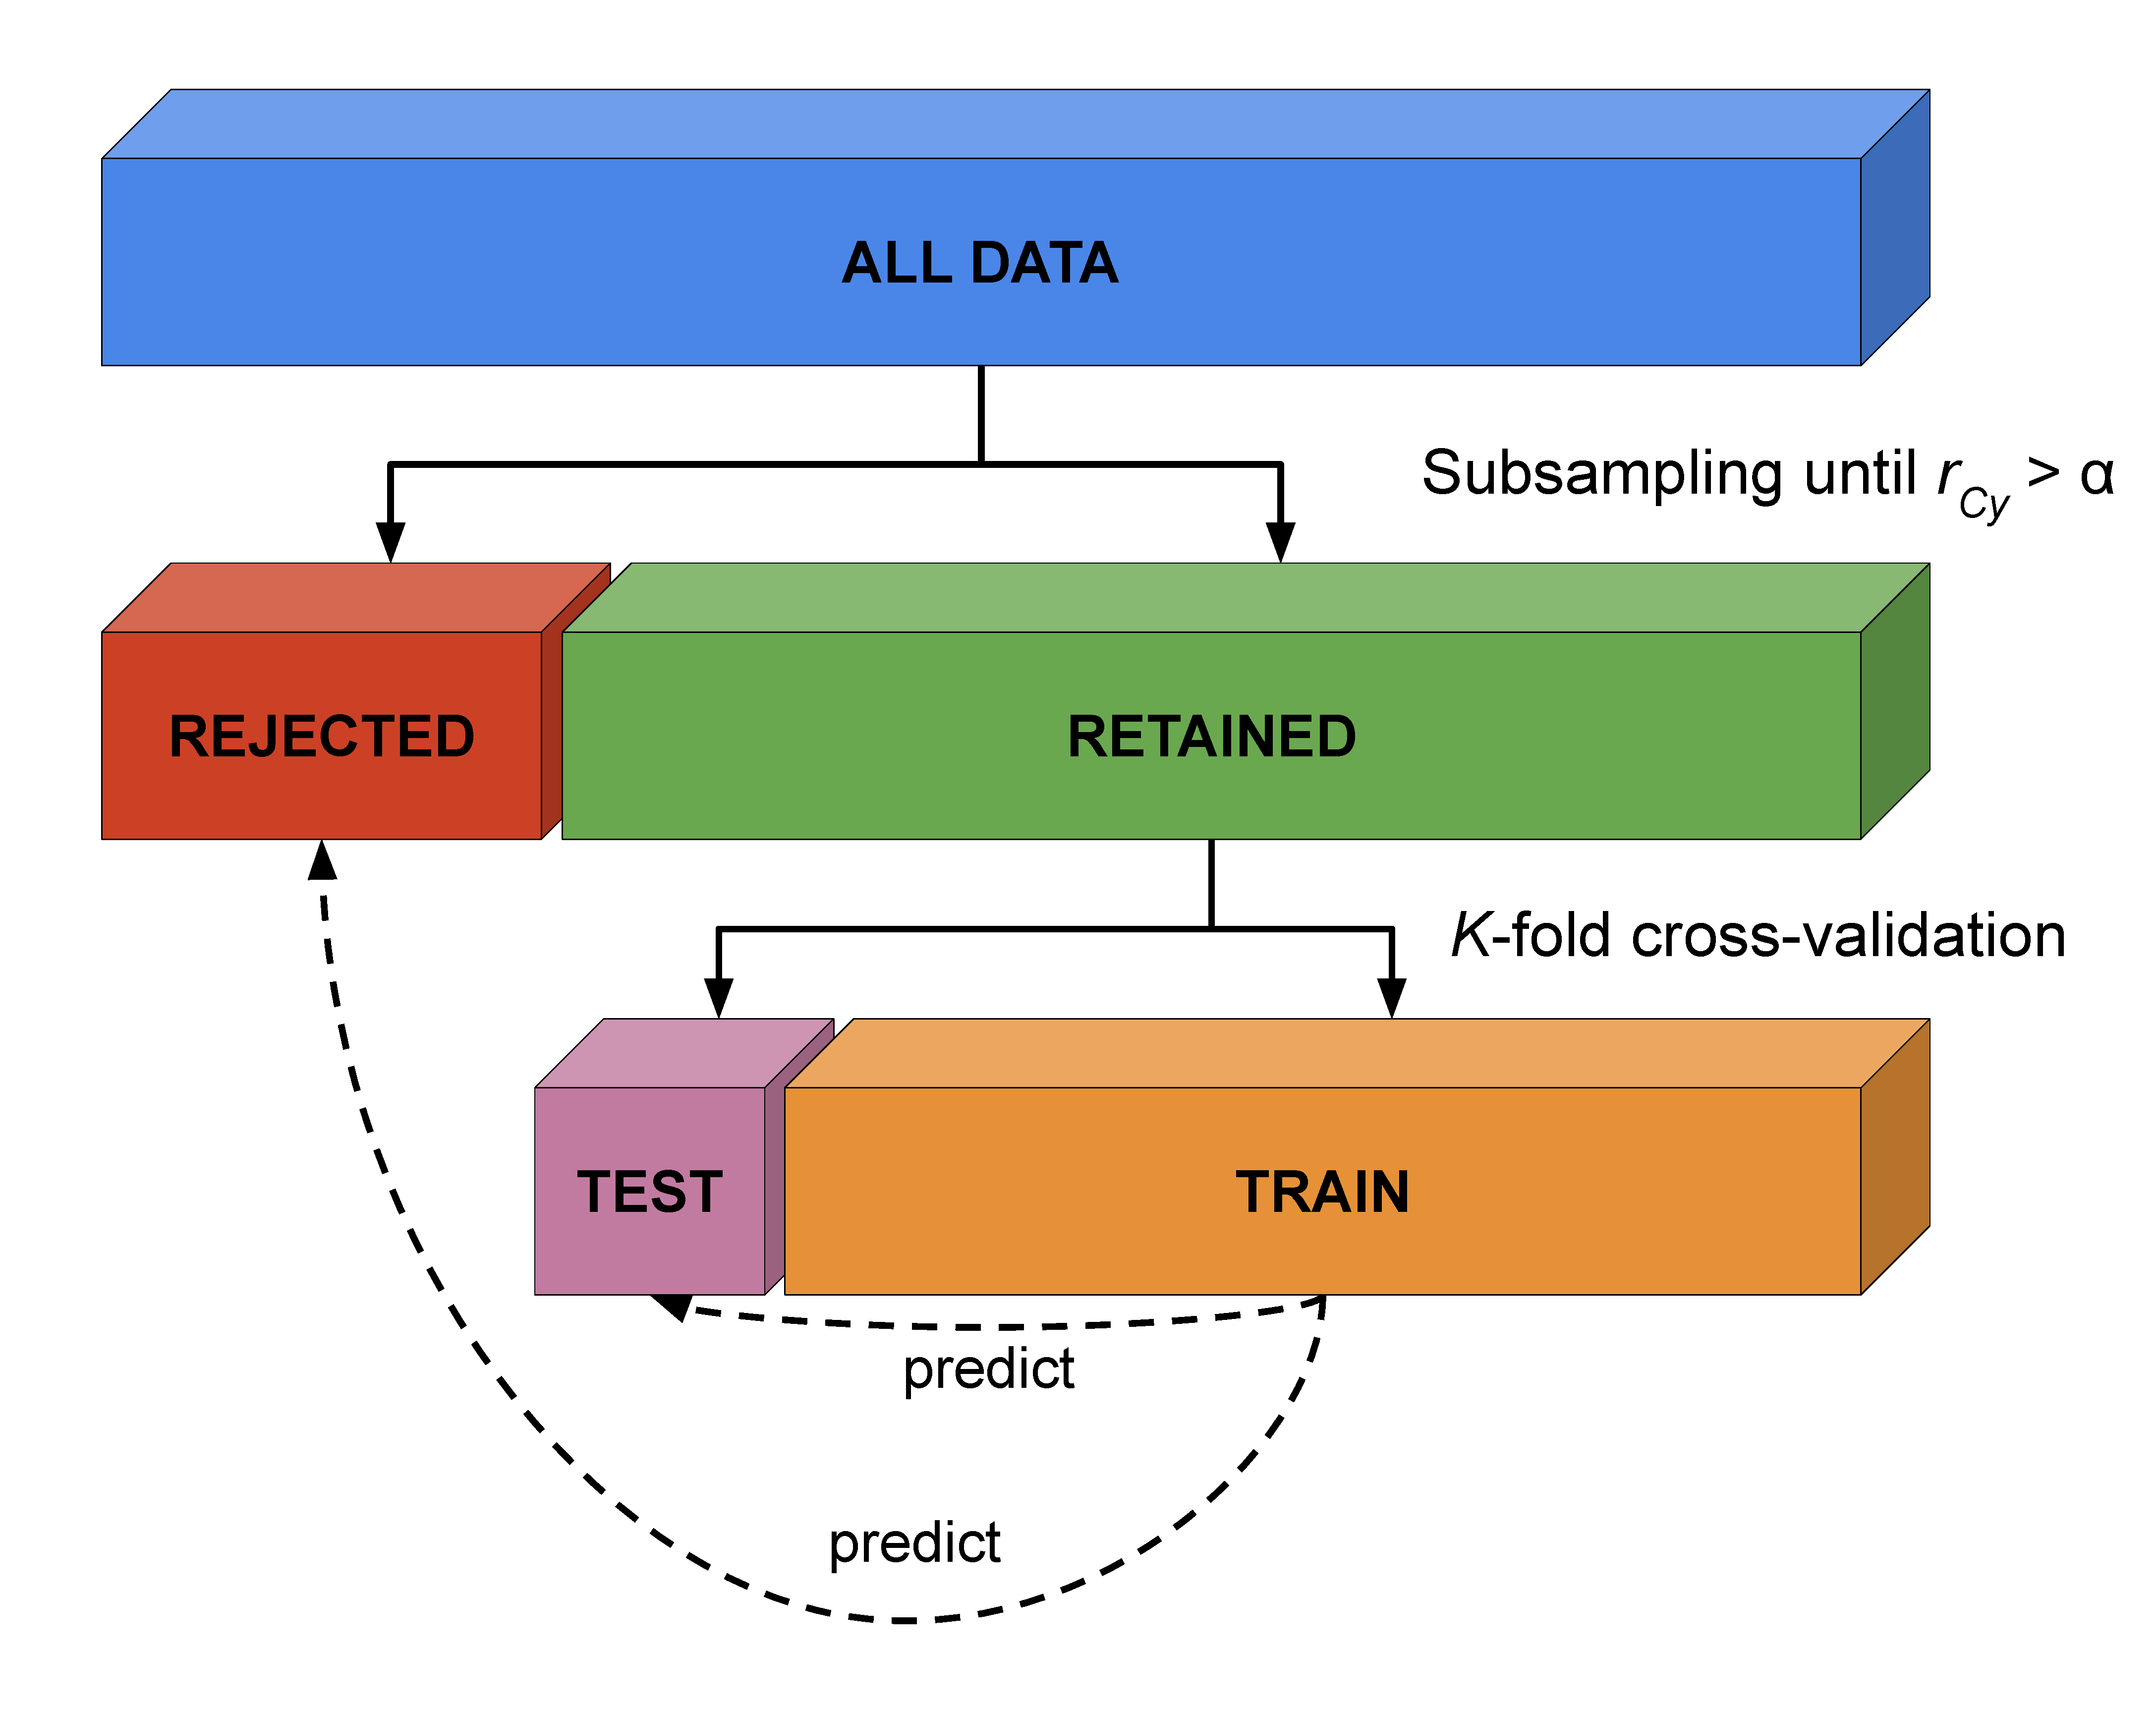
\includegraphics{_bookdown_files/confounds-decoding-files/figures/figure_3.pdf}
\caption{\label{fig:fig-confounds-decoding-3}Visualization of method to evaluate whether counterbalancing yields unbiased cross-validated model performance estimates.}
\end{figure}



\hypertarget{analysis-of-negative-bias-after-wdcr}{%
\subsubsection{Analysis of negative bias after WDCR}\label{analysis-of-negative-bias-after-wdcr}}

As also detailed below, WDCR can lead to significantly below chance accuracy. To investigate the cause of this below chance performance (and to demonstrate that CVCR does not lead to such results), we performed two follow-up simulations. The first follow-up simulation shows that the occurrence of below chance accuracy depends on the distribution of feature-target correlations (\(r_{yX}\); see for a similar argument Jamalabadi et al., \protect\hyperlink{ref-Jamalabadi2016-gr}{2016}), and the second follow-up simulation shows that WDCR artificially narrows this distribution. This artificial narrowing of the distribution is exacerbated both by an increasing number of features (\(K\)), as well as higher correlations between the target and confound (\(r_{Cy}\)).

In the first simulation, we simulated random null data (drawn from a standard normal distribution) with 100 samples (\(N\)) and 200 features (\(K\)), as well as a binary target feature (\(y \in \{0, 1\}\)). We then calculated the cross-validated prediction accuracy using the standard pipeline (without univariate feature selection) described in the \protect\hyperlink{confounds-decoding-methods-pipeline}{Decoding pipeline} section; we iterate this process 500 times. Then, we show that the variance of the cross-validated accuracy is accurately predicted by the standard deviation (i.e., ``width'') of the distribution of correlations between the features and the target (\(r_{yX_{j}}\) with \(j = 1 \dots K\)), which we will denote by \(sd(r_{yX})\). Importantly, we show that below chance accuracy likely occurs when the standard deviation of the feature-target correlation distribution is lower than the standard deviation of the sampling distribution of the Pearson correlation coefficient parameterized with the same number of samples (\(N = 200\)) and the same effect size (i.e., \(\rho = 0\), because we simulated random null data). The sampling distribution of the Pearson correlation coefficient is described by Kendall \& Stuart (\protect\hyperlink{ref-kendall1973functional}{1973}). When \(\rho = 0\) (as in our simulations), the equation is as follows:

\begin{equation}
f(r; N) = (1 -r^2)^{\frac{N-4}{2}}[\mathcal{B}](\frac{1}{2}, \frac{N-2}{2})^{-1}
\end{equation}

where \(\mathcal{B}(a, b)\) represents the Beta-function.

Then, in a second simulation, we similarly simulated null data as in the previous simulation, but now we also generate a continuous confound (\(C\)) with a varying correlation with the target (\(r_{Cy} \in \{0.0, 0.1, 0.2, \dots, 1.0\}\)). Before subjecting the data to the decoding pipeline, we regressed out the confound from the data (i.e., WDCR). We did this for different numbers of features (\(K \in \{1, 5, 10, 50, 100, 500, 1000\}\)). Then, we applied CVCR on the simulated data as well for comparison.

\hypertarget{results}{%
\section{Results}\label{results}}

\hypertarget{influence-of-brain-size}{%
\subsection{Influence of brain size}\label{influence-of-brain-size}}

Before evaluating the different methods for confound control, we determined whether brain size is truly a confound given our proposed definition (``a variable that is not of primary interest, correlates with the target, and is encoded in the neuroimaging data''). We evaluated the relationship between the target and the confound in two ways. First, we calculated the (point-biserial) correlation between gender and brain size, which was significant for both the estimation based on white matter, \(r(216) = .645, p < 0.001\), and the estimation based on grey matter, \(r(216) = .588, p < 0.001\), corroborating the findings by Smith \& Nichols (\protect\hyperlink{ref-Smith2018-th}{2018}). Second, as recommended by Görgen et al. (\protect\hyperlink{ref-Gorgen2017-sy}{2017}), who argue that the potential influence of confounds can be discovered by running a classification analysis using the confound as the (single) feature predicting the target, we ran our decoding pipeline (without univariate feature selection) using brain size as a single feature to predict gender. This analysis yielded a mean classification performance (\(F_{1}\) score) of 0.78 (\emph{SD} = .10) when using brain size estimated from white matter and 0.81 (\emph{SD} = .09) when using brain size estimated from gray matter, which are both significant with \(p < 0.001\) (see Figure \ref{fig:fig-confounds-decoding-4}A).

\begin{figure}
\centering
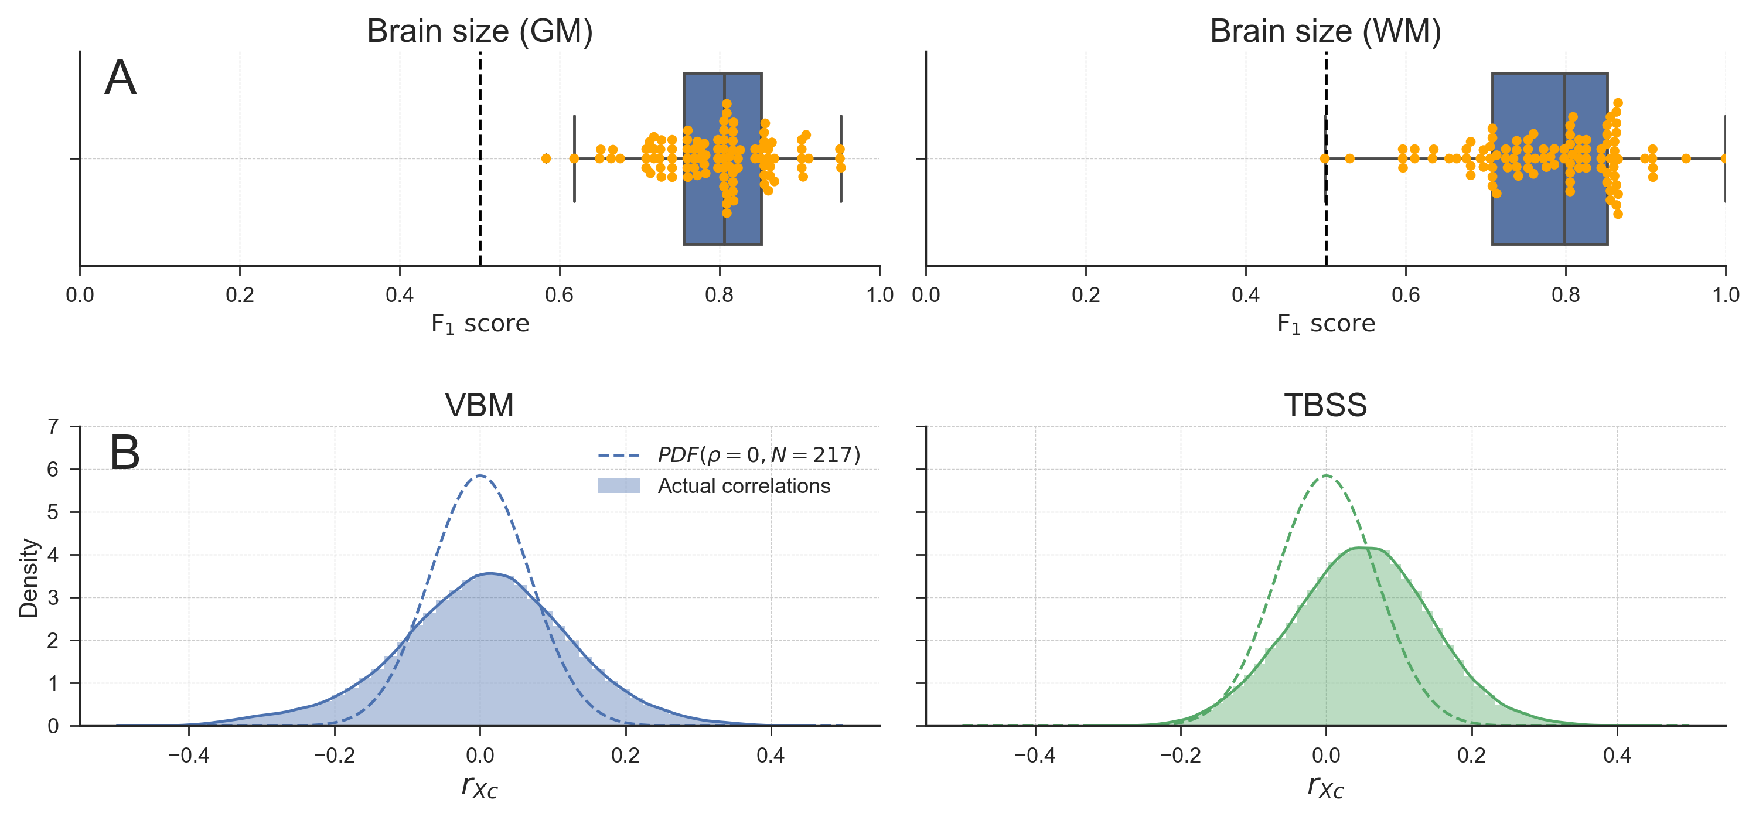
\includegraphics{_bookdown_files/confounds-decoding-files/figures/figure_4.pdf}
\caption{\label{fig:fig-confounds-decoding-4}A) Model performance when using brain size to predict gender for both brain-size estimated from grey matter (left) and from white matter (right). Points in yellow depict individual \(F_{1}\) scores per fold in the 10-fold cross-validation scheme. Whiskers of the box plot are 1.5x the interquartile range. B) Distributions of observed correlations between brain size and voxels (\(r_{XC}\)), overlayed with the analytic sampling distribution of correlation coefficients when \(\rho = 0\) and \(N = 217\), for both the VBM data (left) and TBSS data (right). Density estimates are obtained by kernel density estimation with a Gaussian kernel and Scott's rule (Scott, \protect\hyperlink{ref-scott1979optimal}{1979}) for bandwidth selection.}
\end{figure}



To estimate whether brain size is encoded in the neuroimaging data, we compared the distribution of bivariate correlation coefficients (of each voxel with brain size) with the sampling distribution of correlation coefficients when \(\rho = 0\) and \(N = 217\) (see section \protect\hyperlink{confounds-decoding-results-wdcr-bias}{Analysis of negative bias after WDCR} for details). Under the null hypothesis that there are no correlations between brain size and voxel intensities, each individual correlation coefficient between a voxel and the confound can be regarded as an independent sample with \(N = 217\) (ignoring correlations between voxels for simplicity). Because \(K\) is very large for both the VBM and TBSS data, the empirical distribution of correlation coefficients should, under the null hypothesis, approach the analytic distribution of correlation coefficients parametrized by \(\rho = 0\) and \(N = 217\). Contrarily, the density plots in Fig. \ref{fig:fig-confounds-decoding-4}B clearly show that the observed correlation coefficients distribution does not follow the sampling distribution (with both an increase in variance and a shift of the mode). This indicates that at least some of the correlation coefficients between voxel intensities and brain size are extremely unlikely under the null hypothesis. Note that this interpretation is contingent on the assumption that the relation between brain size and VBM/TBSS data is linear. In the Supplementary Materials and Results (Supplementary Figures \ref{fig:fig-confounds-decoding-S7}-\ref{fig:fig-confounds-decoding-S9}), we provide some evidence for the validity of this assumption.

\hypertarget{baseline-model-no-confound-control}{%
\subsection{Baseline model: no confound control}\label{baseline-model-no-confound-control}}

In our baseline model on the empirical data, for different numbers of voxels, we predicted gender from structural MRI data (VBM and TBSS) without controlling for brain size (see Figure \ref{fig:fig-confounds-decoding-5}). The results show significant above chance performance of the MVPA pipeline based on both the VBM data and the TBSS data. All performance scores averaged across folds were significant (\(p < 0.001\)).

\begin{figure}
\centering
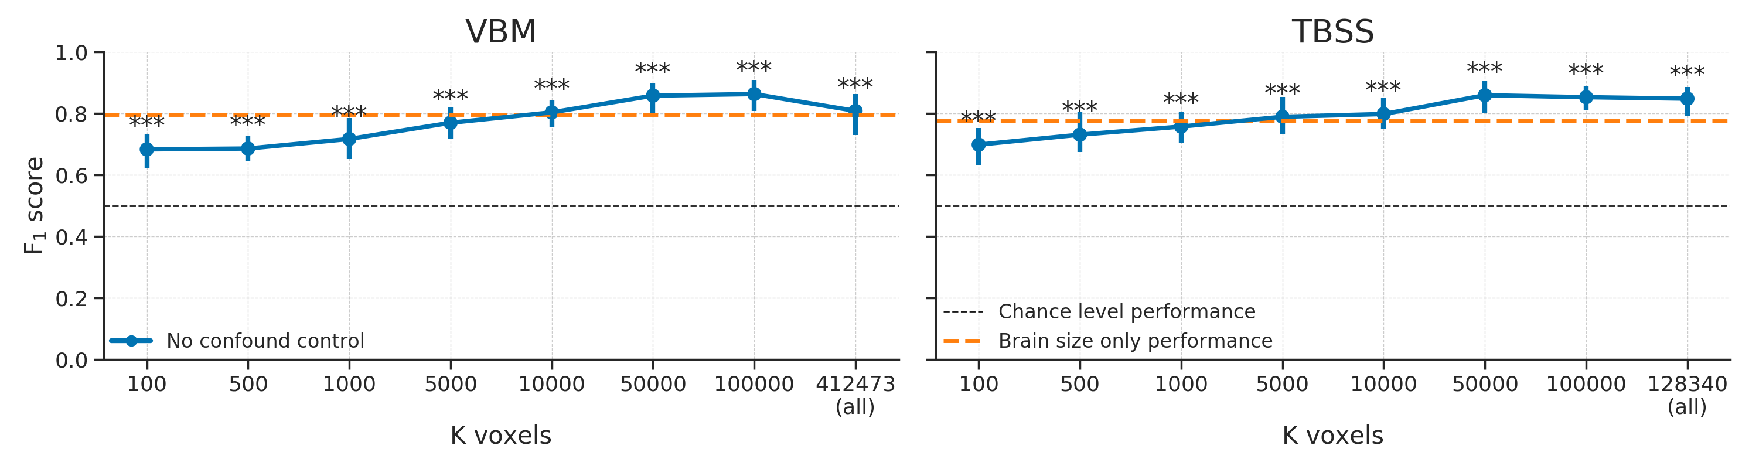
\includegraphics{_bookdown_files/confounds-decoding-files/figures/figure_5.pdf}
\caption{\label{fig:fig-confounds-decoding-5}Baseline scores using the VBM (left) and TBSS (right) data without any confound control. Scores reflect the average \(F_{1}\) score across 10 folds; error bars reflect 95\% confidence intervals. The dashed black line reflect theoretical chance-level performance and the dashed orange line reflects the average model performance when only brain size is used as a predictor for reference; Asterisks indicates significant performance above chance: *** = \(p < 0.001\), ** = \(p < 0.01\), * = \(p < 0.05\).}
\end{figure}



These above chance performance estimates replicate previous studies on gender decoding using structural MRI data (Del Giudice et al., \protect\hyperlink{ref-Del_Giudice2016-ns}{2016}; Rosenblatt, \protect\hyperlink{ref-Rosenblatt2016-oy}{2016}; Sepehrband et al., \protect\hyperlink{ref-Sepehrband2018-dy}{2018}) and will serve as a baseline estimate of model performance to which the confound control methods will be compared.

In the next three subsections, we will report the results from the three discussed methods to control for confounds: post hoc counterbalancing, whole-dataset confound regression (WDCR), and cross-validated confound regression (CVCR).

\hypertarget{post-hoc-counterbalancing}{%
\subsection{Post hoc counterbalancing}\label{post-hoc-counterbalancing}}

\hypertarget{empirical-results}{%
\subsubsection{Empirical results}\label{empirical-results}}

In order to decorrelate brain size and gender (i.e., \(r_{Cy} > 0.1\)), our subsampling algorithm selected 117 samples in the VBM data (i.e., a sample size reduction of 46.1\%) and 131 samples in the TBSS data (i.e., a reduction of 39.6\%). The model performance for different values of (number of voxels) are shown in Figure \ref{fig:fig-confounds-decoding-6}. Contrary to our expectations, the predictive accuracy of our decoding pipeline after counterbalancing was similar to baseline performance. This is particularly surprising in light of the large reductions in sample size, which results in a substantial loss in power, which in turn is expected to lead to lower model performance.

\begin{figure}
\centering
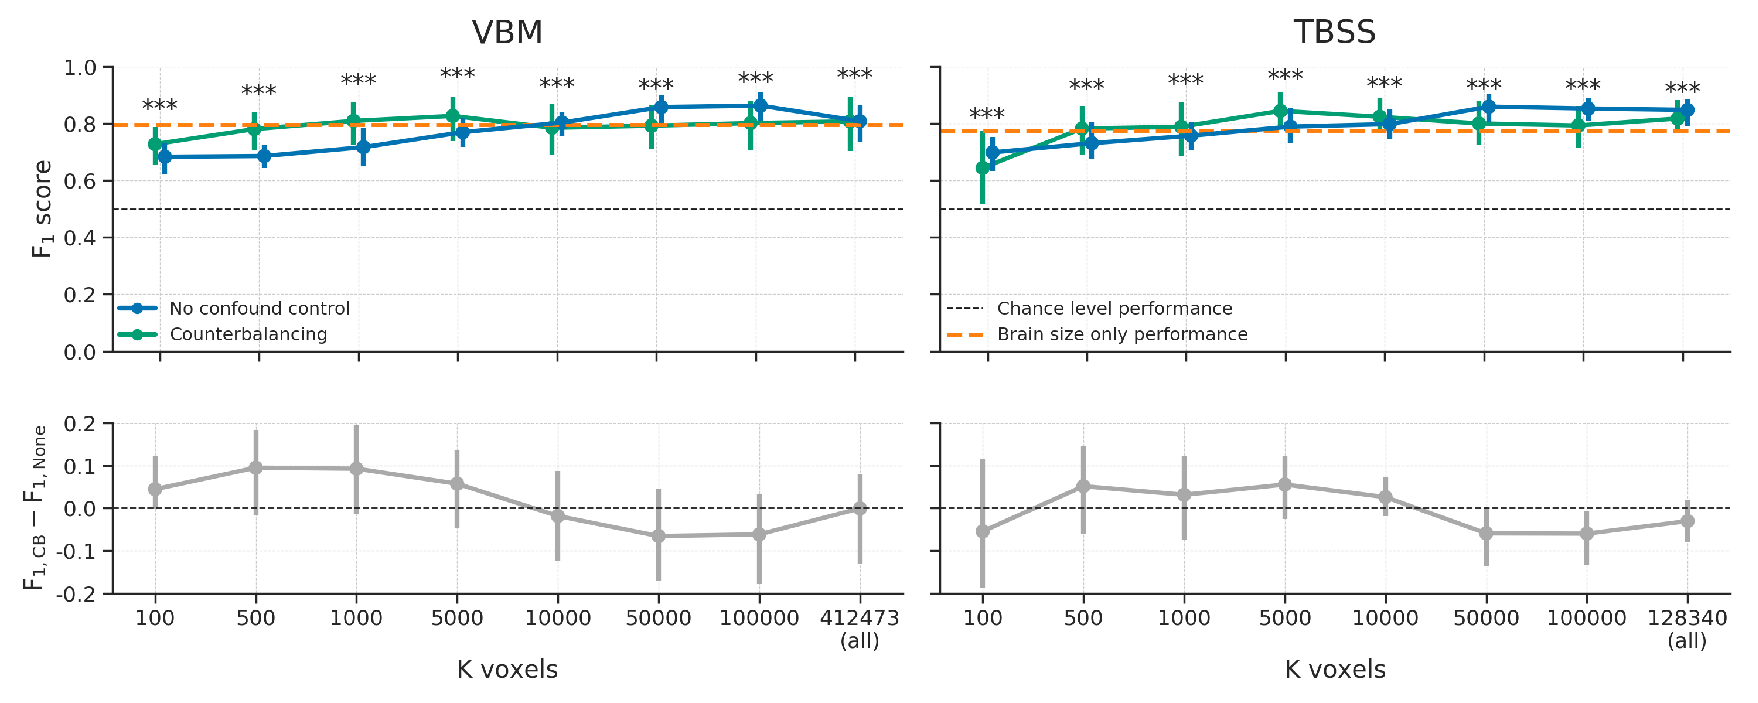
\includegraphics{_bookdown_files/confounds-decoding-files/figures/figure_6.pdf}
\caption{\label{fig:fig-confounds-decoding-6}Model performance after counterbalancing (green) versus the baseline performance (blue) for both the VBM (left) and TBSS (right) data (upper row) and the difference in performance between the methods (lower row). Performance reflects the average (difference) \(F_{1}\) score across 10 folds; error bars reflect 95\% confidence intervals. The dashed black line reflect theoretical chance-level performance (0.5) and the dashed orange line reflects the average model performance when only brain size is used as a predictor. Asterisks indicates significant performance above chance: *** = \(p < 0.001\), ** = \(p < 0.01\), * = \(p < 0.05\).}
\end{figure}



One could argue that the lack of expected decrease in model performance after counterbalancing can be explained by the possibility that the subsampling and counterbalancing procedure just leads to the selection of different features during univariate feature selection compared to the baseline model. In other words, the increase in model performance may be caused by the feature selection function, which selects ``better'' voxels (i.e., containing more ``robust'' signal), resulting in similar model performance in spite of the reduction in sample size. However, this does not explain the similar scores for counterbalancing and the baseline model when using all voxels (the data points at \(K \mathrm{voxels} = \dots \mathrm{(all)}\) in Figure \ref{fig:fig-confounds-decoding-6}). Another possibility for the relative increase in model performance based on the counterbalanced data versus the baseline model is that counterbalancing increased the amount of signal in the data. Indeed, counterbalancing appeared to increase the (absolute) correlations between the data and the target (\(r_{yX}\)), which is visualized in Figure \ref{fig:fig-confounds-decoding-7}, suggesting an increase in signal.

\begin{figure}
\centering
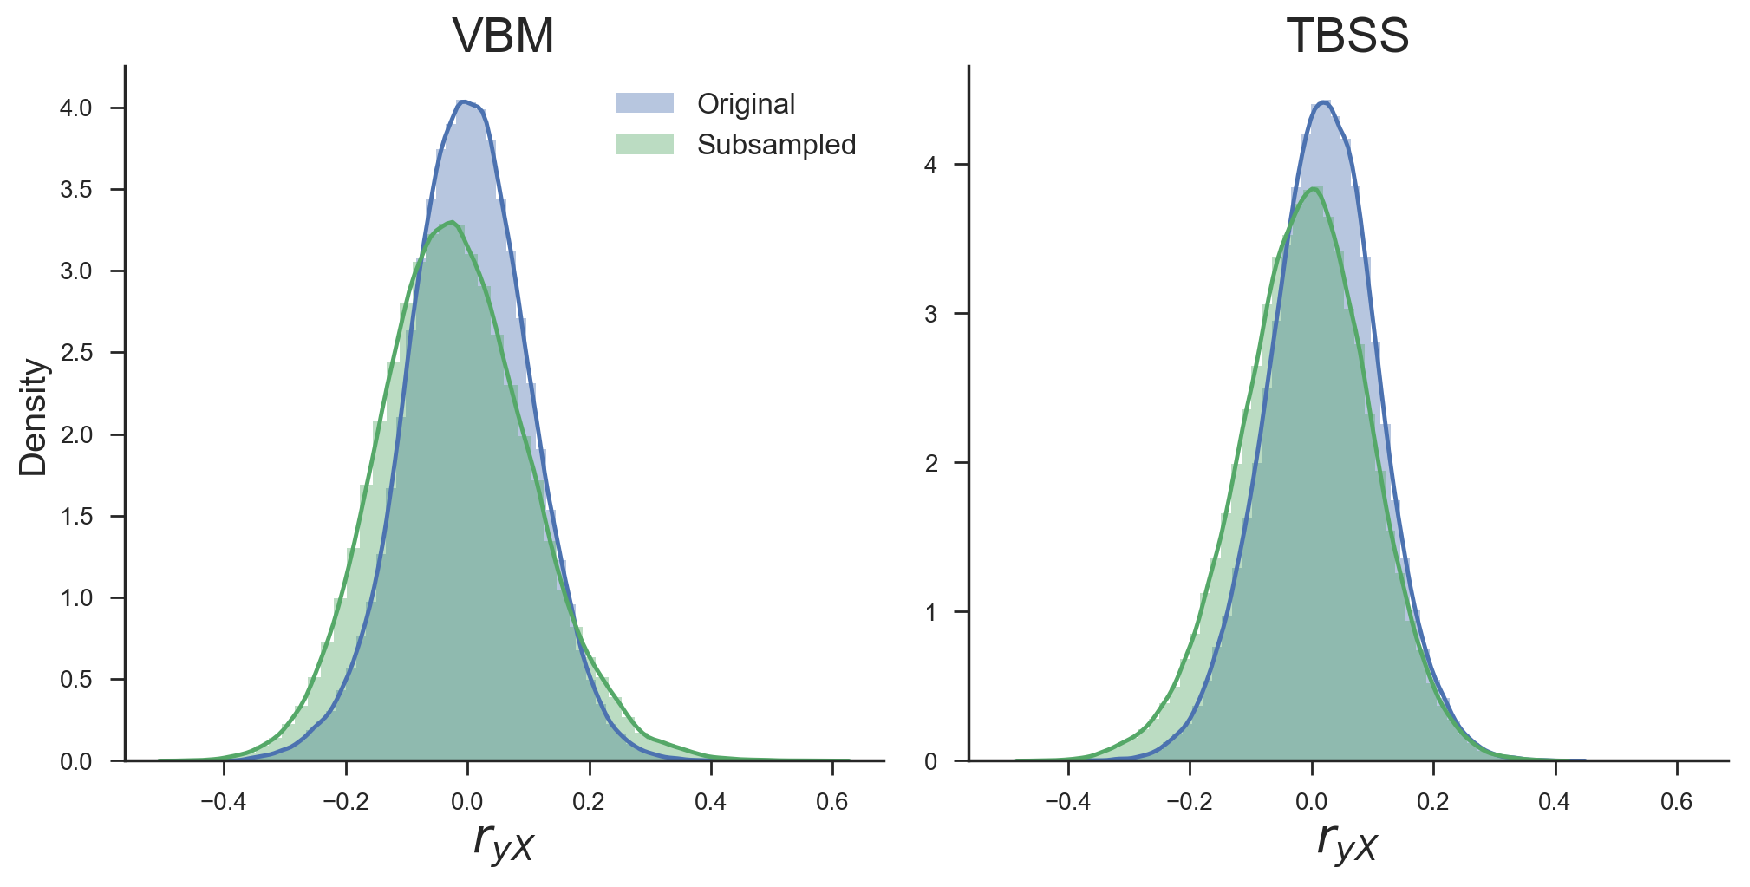
\includegraphics{_bookdown_files/confounds-decoding-files/figures/figure_7.pdf}
\caption{\label{fig:fig-confounds-decoding-7}Density plots of the correlations between the target and voxels across all voxels before (blue) and after (green) subsampling for both the VBM and TBSS data. Density estimates are obtained by kernel density estimation with a Gaussian kernel and Scott's rule (Scott, \protect\hyperlink{ref-scott1979optimal}{1979}) for bandwidth selection.}
\end{figure}



This apparent increase in the correlations between the target and neuroimaging data goes against the intuition that removing the influence of a confound that is highly correlated with the target will reduce decoding performance. To further investigate this, we replicated this effect of post hoc counterbalancing on simulated data, as described in the next section (\protect\hyperlink{confounds-decoding-results-cb-efficacy}{Efficacy analyses}), and additionally investigated the cause of the negative bias observed after WDCR using a separate set of simulations.

\hypertarget{confounds-decoding-results-cb-efficacy}{%
\subsubsection{Efficacy analysis}\label{confounds-decoding-results-cb-efficacy}}

To evaluate the efficacy of the three confound control methods, we simulated data in which we varied the strength of confound \(R^2\) and signal \(R^2\), after which we applied the three confound control methods to the data. The results of this analysis show that counterbalancing maintains chance-level model performance when there is almost no signal in the data (i.e., signal \(R^2 = 0.004\); Figure \ref{fig:fig-confounds-decoding-8}, left graph, green line). However, when there is some signal (i.e., signal \(R^2 = 0.1\); Fig. 8, right graph), we observed that counterbalancing yields similar or even higher scores than the baseline model, replicating the effects observed in the empirical analyses.

\begin{figure}
\centering
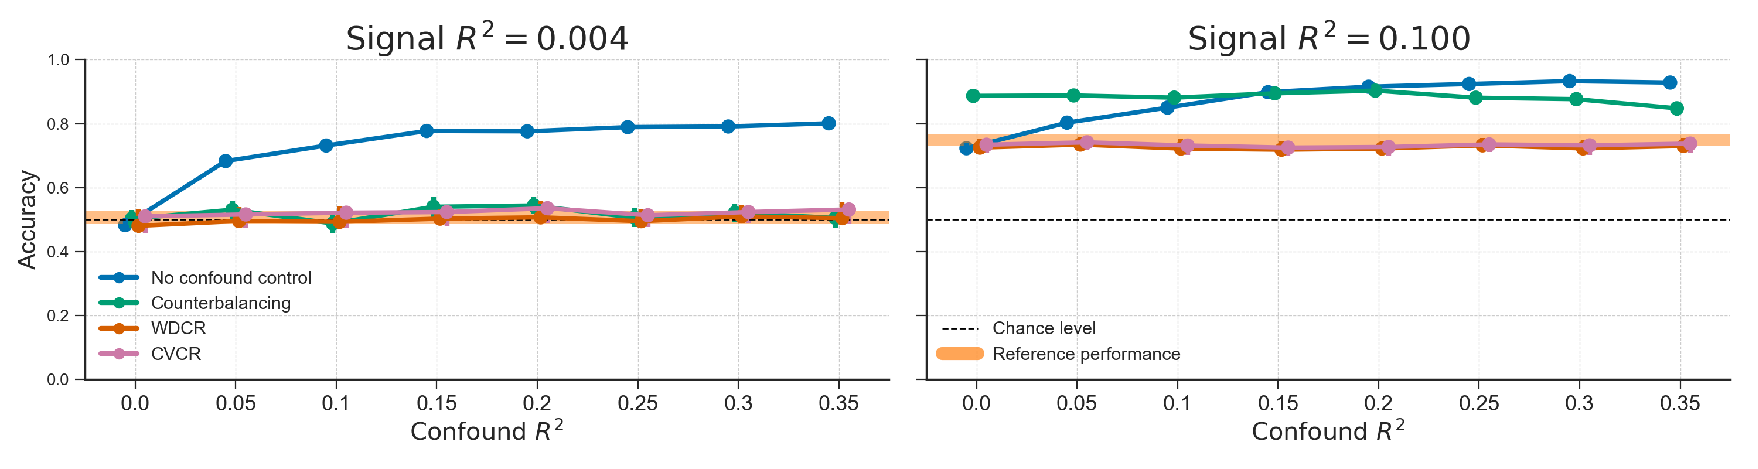
\includegraphics{_bookdown_files/confounds-decoding-files/figures/figure_8.pdf}
\caption{\label{fig:fig-confounds-decoding-8}Results from the different confound control methods on simulated data without any experimental effect (signal \(R^2 = 0.004\); left graph) and with some experimental effect (signal \(R^2 = 0.1\); right graph) for different values of confound \(R^2\). The orange line represents the average performance (±1 SD) when confound \(R^2 = 0\), which serves as a ``reference performance'' for when there is no confounded signal in the data. For both graphs, the correlation between the target and the confound, \(r_{yC}\), is fixed at 0.65. The results from the WDCR and CVCR methods are explained later.}
\end{figure}



As is apparent from Figure \ref{fig:fig-confounds-decoding-8} (right panel), when there is some signal, the counterbalanced data seem to yield better performance than the baseline model only for relatively low confound \(R^2\) values (confound \(R^2 < 0.15\)). As suggested by our findings in the empirical data (see Figure \ref{fig:fig-confounds-decoding-7}), we hypothesized that the observed improvement in model performance after counterbalancing was caused by the increase in correlations between the target and features in the neuroimaging data. In support of this hypothesis, Figure \ref{fig:fig-confounds-decoding-9} illustrates the relations between the strength of the confound (confound \(R^2\), color coded), the increase in correlations after post hoc counterbalancing (\(\delta r_{yX} = r_{yX}^{\mathrm{after}} - r_{yX}^{\mathrm{after}}\); x-axis) for each confound \(R^2\), and the resulting difference in model performance (\(\mathrm{ACC}_{\mathrm{CB}} - \mathrm{ACC}_{\mathrm{baseline}}\); y-axis). The figure shows that the increase or decrease in accuracy after counterbalancing (compared to baseline) depends on \(\delta r_{yX}\) (\(r(79) = .922\), \(p < 0.001\)), which in turn depends on confound \(R^2\) (\(r(79) = -0.987\), \(p < 0.001\)). To reiterate, these differences in model performance are only due to the post hoc counterbalancing procedure and not due to varying signal in the simulated data. The effect of post hoc counterbalancing on model performance thus seems to depend on the strength of the confound.

\begin{figure}
\centering
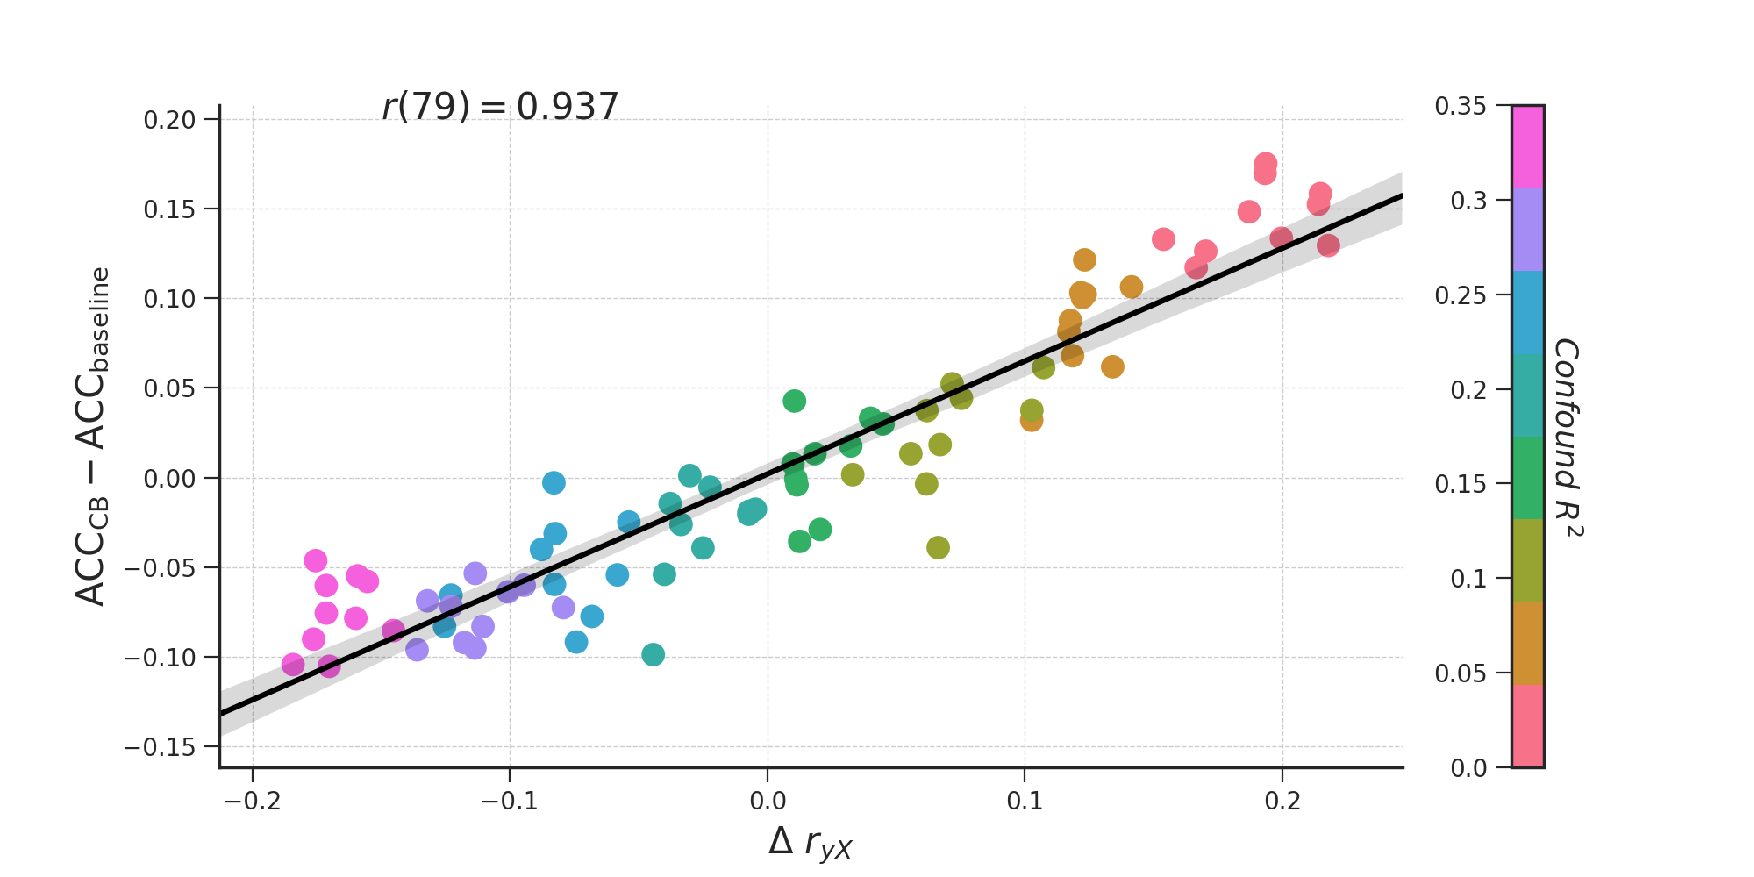
\includegraphics{_bookdown_files/confounds-decoding-files/figures/figure_9.pdf}
\caption{\label{fig:fig-confounds-decoding-9}The relationship between the increase in correlations between target and data (\(r_{yX}\)) after subsampling, confound \(R^2\), difference in model performance (here: accuracy) between the counterbalance model and baseline model (\(\mathrm{ACC}_{\mathrm{CB}} - \mathrm{ACC}_{\mathrm{baseline}}\)).}
\end{figure}



While this relationship in Figure \ref{fig:fig-confounds-decoding-9} might be statistically interesting, it does not explain why post hoc counterbalancing tends to increase the correlations between neuroimaging data and target, and even outperforms the baseline model when confound \(R^2\) is low and some signal is present. More importantly, it does not tell us whether the post hoc counterbalancing procedure uncovers signal that is truly related to the target --- in which case the procedure suppresses noise --- or inflates performance estimates and thereby introduces positive bias. Therefore, in the next section, we report and discuss results from a follow-up simulation that intuitively shows why post hoc counterbalancing leads to an increase in performance, and furthermore shows that this increase is in fact a positive bias.

\hypertarget{analysis-of-positive-bias-after-post-hoc-counterbalancing}{%
\subsubsection{Analysis of positive bias after post hoc counterbalancing}\label{analysis-of-positive-bias-after-post-hoc-counterbalancing}}

With this follow-up analysis, we aimed to visualize the scenario in which post hoc counterbalancing leads to a clearly better performance than model performance without confound control. As such, we generated 1000 data sets using a covariance matrix that we knew leads to a large difference between the baseline model and model performance after counterbalancing (i.e., data with a low confound \(R^2\)). From these 1000 datasets, we selected the dataset that yielded the largest difference for our visualization (see the \protect\hyperlink{confounds-decoding-methods-counterbalancing-bias}{Analysis of positive bias after post hoc counterbalancing} section in the Methods for details).

The data that yielded the largest difference (i.e., a performance increase from 0.613 to 0.804, a 31\% increase) are visualized in Figure \ref{fig:fig-confounds-decoding-10}. Each sample's confound value (\(C\)) is plotted against its feature value (\(X\)), both before subsampling (upper scatter plot) and after subsampling (lower scatter plot). From visual inspection, it appears that the samples rejected by the subsampling procedure (i.e., the samples with the white border) have relatively large absolute values of the confound variable, which tend to lie close to or on the ``wrong'' side of the classification boundary (i.e., the dashed black line) in this specific configuration of the data. In other words, subsampling seems to reject samples that are harder to classify or would be incorrectly classified based on the data (here, the single feature of \(X\)). The density plots in Figure \ref{fig:fig-confounds-decoding-10} show the same effect in a different way: while the difference in the modes of the distributions of the confound (\(C\)) between classes is reduced after subsampling (i.e., the density plots parallel to the y-axis), the difference in the modes of the distributions of the data (\(X\)) between classes is actually increased after subsampling (i.e., the density plots parallel to the x-axis).

\begin{figure}
\centering
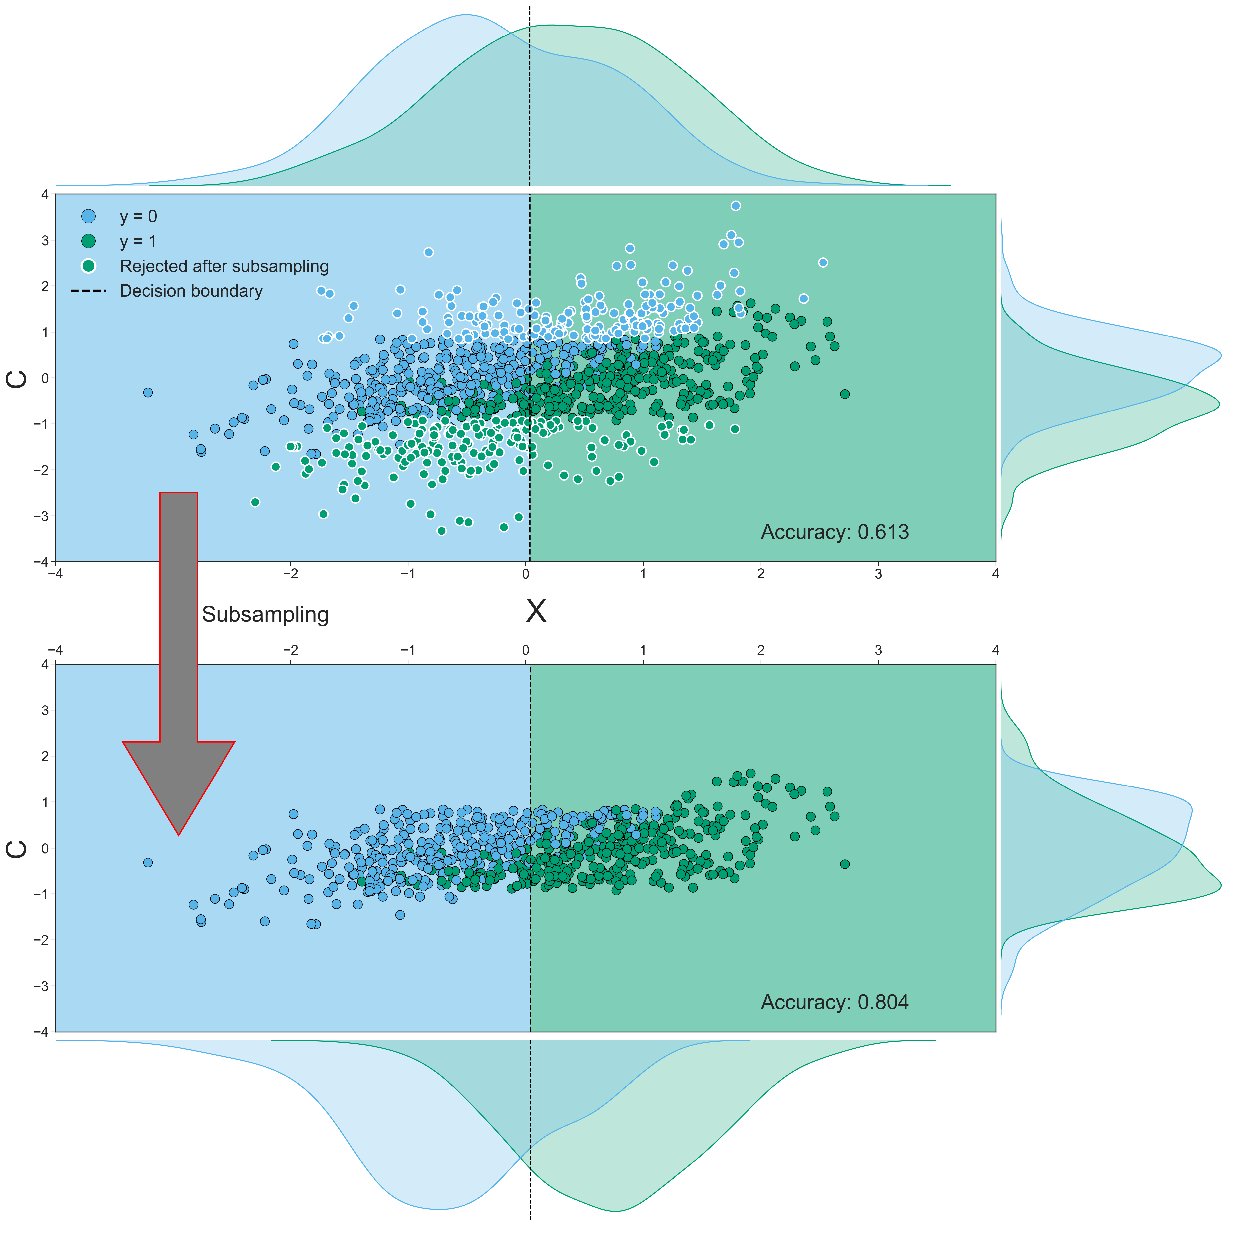
\includegraphics{_bookdown_files/confounds-decoding-files/figures/figure_10.pdf}
\caption{\label{fig:fig-confounds-decoding-10}Both scatterplots visualize the relationship between the data (\(X\) with \(K=1\), on the x-axis), the confound (\(C\), on the y-axis) and the target (\(y\)). Dots with a white border in the upper scatterplot indicate samples that are rejected in the subsampling process; the lower scatterplot visualizes the data without these rejected samples. The dashed black lines in the scatterplot represent the decision boundary of the SVM classifier; the color of the background shows how samples in that area are classified (a blue background means a prediction of \(y = 0\) and a green background means a prediction of \(y = 1\)). The density plots parallel to the y-axis depict the distribution of the confound (\(C\)) for the samples in which \(y = 0\) (blue) and in which \(y = 1\) (green). The density plots parallel to x-axis depict the distribution of the data (\(X\)) for the samples in which \(y = 0\) (blue) and in which \(y = 1\) (green). Density estimates are obtained by kernel density estimation with a Gaussian kernel and Scott's rule (Scott, \protect\hyperlink{ref-scott1979optimal}{1979}) for bandwidth selection.}
\end{figure}



We quantified this effect of subsampling by comparing the signed distance from the decision boundary (i.e., the dashed line in the upper scatter plot) between the retained samples and the rejected (subsampled) samples, in which a larger distance from the decision boundary reflects a higher confidence of the classifier's prediction (see Figure \ref{fig:fig-confounds-decoding-3} for a visualization of this method). Indeed, we found that samples that are removed by subsampling lie significantly closer to (or on the ``wrong'' side of) the decision boundary (\emph{M} = -.358, \emph{SD} = .619) than samples that are retained after subsampling (\emph{M} = .506, \emph{SD} = .580), as indicated by a independent samples \emph{t}-test, \(t(998) = 22.32\), \(p < 0.001\). Also (which follows from the previous observation), samples that would have been removed by subsampling are more often classified incorrectly (75\% incorrect) than the samples that would have been retained by subsampling (20\% incorrect), as indicated by a chi-squared test, \(\chi^{2} = 270.29\), \(p < 0.001\).

To show that the same effect (i.e., removing samples that tend to be hard to classify or would be wrongly classified) occurred in the empirical data after counterbalancing as well, we applied the same analysis of comparing model performance and distance to boundary between the retained and rejected samples to the empirical data. Indeed, across all different numbers of voxels (\(K\)), the retained samples were significantly more often classified correctly (Figure \ref{fig:fig-confounds-decoding-11}A) and had a significantly larger distance to the classification boundary (Figure \ref{fig:fig-confounds-decoding-11}B) than the rejected samples. This demonstrates that the same effect of post hoc counterbalancing, as shown in the simulated data, likely underlies the increase in model performance of the counterbalanced data relative to the baseline model in the empirical data.

\begin{figure}
\centering
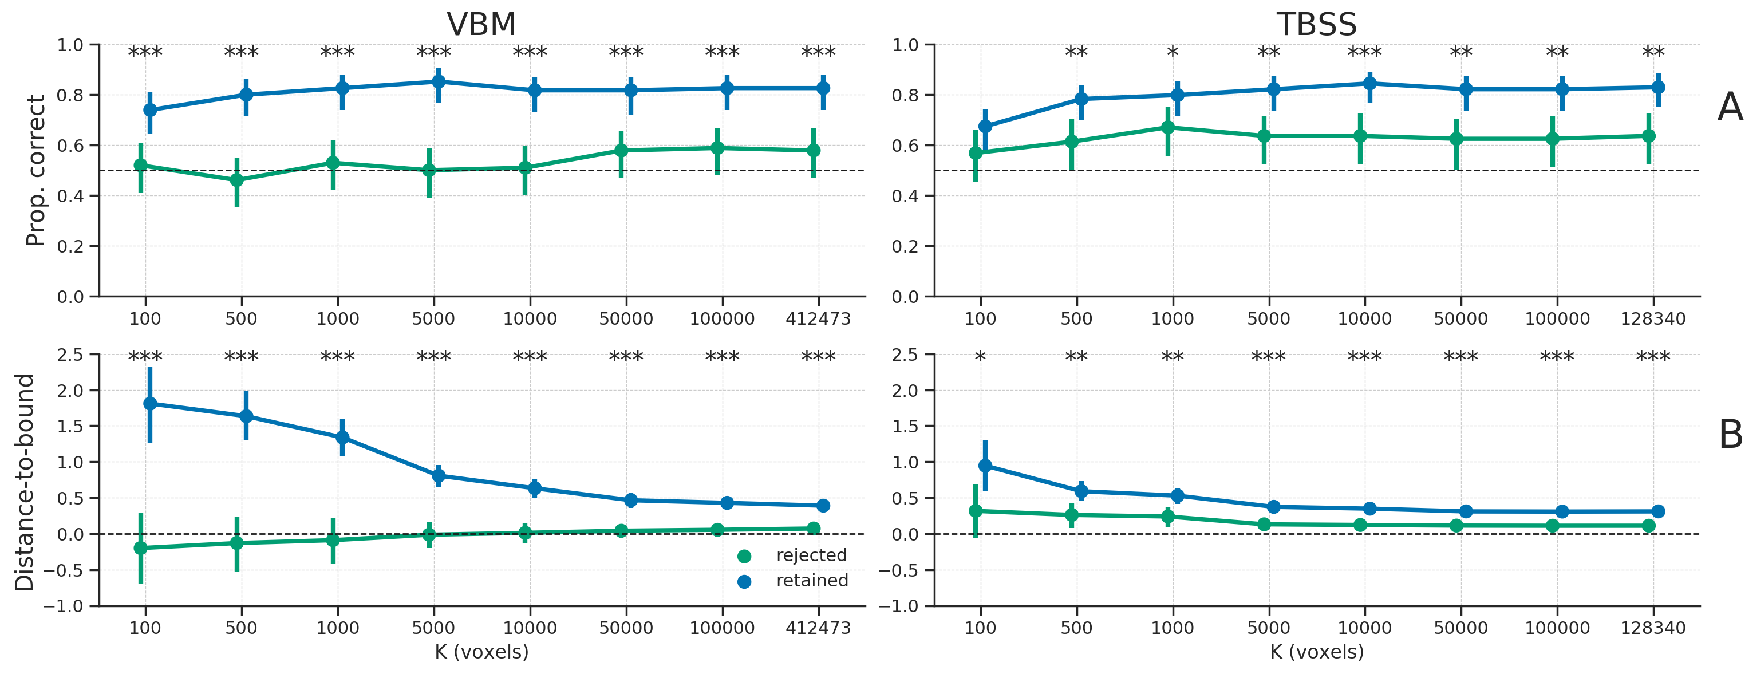
\includegraphics{_bookdown_files/confounds-decoding-files/figures/figure_11.pdf}
\caption{\label{fig:fig-confounds-decoding-11}\textbf{A}) The proportion of samples classified correctly, separately for the ``retained'' samples (blue line) and ``rejected'' samples (green line); the dashed line represents chance level (0.5). \textbf{B}) The average distance to the classification boundary for the retained and rejected samples; the dashed line represents the decision boundary, with values below the line representing samples on the ``wrong'' side of the boundary (and vice versa). Asterisks indicates a significant difference between the retained and rejected samples: *** = \(p < 0.001\), ** = \(p < 0.01\), * = \(p < 0.05\).}
\end{figure}



One can wonder how much the occurrence of these observed biases in post hoc counterbalancing depends on the specific method of subsampling used. Random subsampling led to qualitatively similar results as targeted subsampling (cf.~Supplementary Figures \ref{fig:fig-confounds-decoding-S13} and \ref{fig:fig-confounds-decoding-S14} with random subsampling). Instead, the bias is introduced through features that weakly correlate with the target in the whole sample, but strongly in subsamples where there is no correlation between target and the confound (features which, as our results show, exist in the neuroimaging data). That is, the bias is an indirect result of decorrelating target and confound in the sample, which is an essential step in post hoc counterbalancing (in fact, it is the \emph{goal} of counterbalancing). For this reason, we consider it unlikely (but not impossible) that there exists a way to subsample data without introducing biases.

In summary, removing a subset of observations to correct for the influence of a confound can induce substantial bias by removing samples that are harder to classify using the available data. The bias itself can be subtle (e.g., in our empirical results, the predictive performance falls in a realistic range of predictive performances), and could remain undetected when present. Therefore, we believe that post hoc counterbalancing by subsampling the data is an inappropriate method to control for confounds.

\hypertarget{whole-dataset-confound-regression-wdcr}{%
\subsection{Whole-dataset confound regression (WDCR)}\label{whole-dataset-confound-regression-wdcr}}

\hypertarget{empirical-results-1}{%
\subsubsection{Empirical results}\label{empirical-results-1}}

In addition to post hoc counterbalancing, we evaluated the efficacy of ``whole-dataset confound regression'' (WDCR), i.e.~regressing out the confound from each feature separately using all samples from the dataset to control for confounds. Compared to the baseline model, WDCR yielded a strong decrease in performance, even dropping (significantly) below chance for all TBSS analyses and a subset of the VBM analyses (see Figure \ref{fig:fig-confounds-decoding-12}).

\begin{figure}
\centering
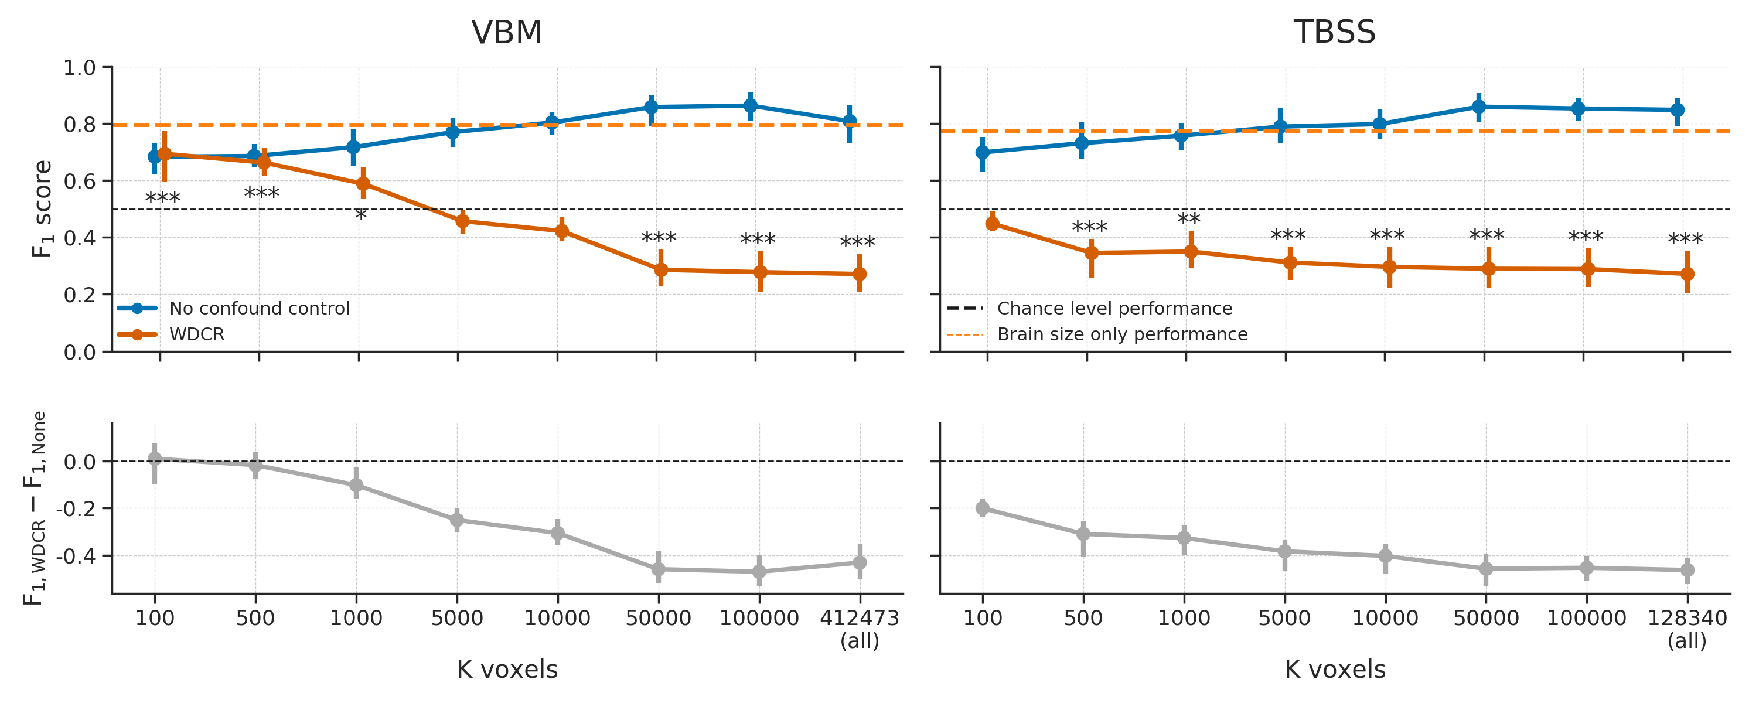
\includegraphics{_bookdown_files/confounds-decoding-files/figures/figure_12.pdf}
\caption{\label{fig:fig-confounds-decoding-12}Model performance after WDCR (orange) versus the baseline performance (blue) for both the VBM (left) and TBSS (right) data. Performance reflects the average \(F_{1}\) score across 10 folds; error bars reflect 95\% confidence intervals. The dashed black line reflect theoretical chance-level performance (0.5) and the dashed orange line reflects the average model performance when only brain size is used as a predictor. Asterisks indicates performance of the WDCR model that is significantly above or below chance: *** = \(p < 0.001\), ** = \(p < 0.01\), * = \(p < 0.05\).}
\end{figure}



This strong (and implausible) reduction in model performance after WDCR is investigated in more detail in the next two sections on the results from the simulations.

\hypertarget{efficacy-analysis}{%
\subsubsection{Efficacy analysis}\label{efficacy-analysis}}

The results from the analyses investigating the efficacy of the confound control methods (see Figure \ref{fig:fig-confounds-decoding-8}) show that WDCR accurately corrects for the confound in both in data without signal (i.e., when signal \(R^2 = 0.004\)) and in data with some signal (i.e., when signal \(R^2 = 0.1\)), as evident from the fact that the performance after WDCR is similar to the reference performance. This result (i.e., plausible performance after confound control) stands in contrast to the results from the empirical analyses, which is why we ran a follow-up analysis on simulated data to investigate this specific issue.

\hypertarget{confounds-decoding-results-wdcr-bias}{%
\subsubsection{Analysis of negative bias after WDCR}\label{confounds-decoding-results-wdcr-bias}}

Inspired by the work of Jamalabadi et al. (\protect\hyperlink{ref-Jamalabadi2016-gr}{2016}) on below chance accuracy in decoding analyses, we ran several follow-up analyses to get insight into why WDCR leads to below chance model performance. As Jamalabadi et al.~show, below chance model performance occurs when the data contain little signal. In our first follow-up simulation, we sought to refine the explanation of the cause of below chance model performance by linking it to the observed standard deviation of the empirical distribution of correlations between the data (\(X\)) and the target (\(y\)). To do so, we simulated random data (\(X\)) and a binary target (\(y \in \{0, 1\}\)) and estimated (per fold) the cross-validated classification accuracy using the standard pipeline described in the methods section. We repeated this process 500 times, yielding 500 data sets. The expected \emph{average} predictive accuracy for each dataset is 0.5, but this varies randomly across folds and iterations. We hypothesized that this variance can be explained by the standard deviation (``width'') of the initial feature-target correlation distribution, \emph{sd}(\(r_{Xy}\)): narrower distributions may yield relatively lower cross-validated classification accuracy than relatively wider feature-target correlation distributions. Indeed, we find that the initial standard deviation of this distribution is significantly correlated with the cross-validated accuracy, \(r(499) = 0.73\), \(p < 0.001\) (Figure \ref{fig:fig-confounds-decoding-13}A). Importantly, we find that this relationship holds for different values of \(N\) (see Supplementary Figure \ref{fig:fig-confounds-decoding-S15}, for different sizes of the test set (see Supplementary Figure \ref{fig:fig-confounds-decoding-S16}), and for different sizes of \(K\) (see Supplementary Figure \ref{fig:fig-confounds-decoding-S17}).

\begin{figure}
\centering
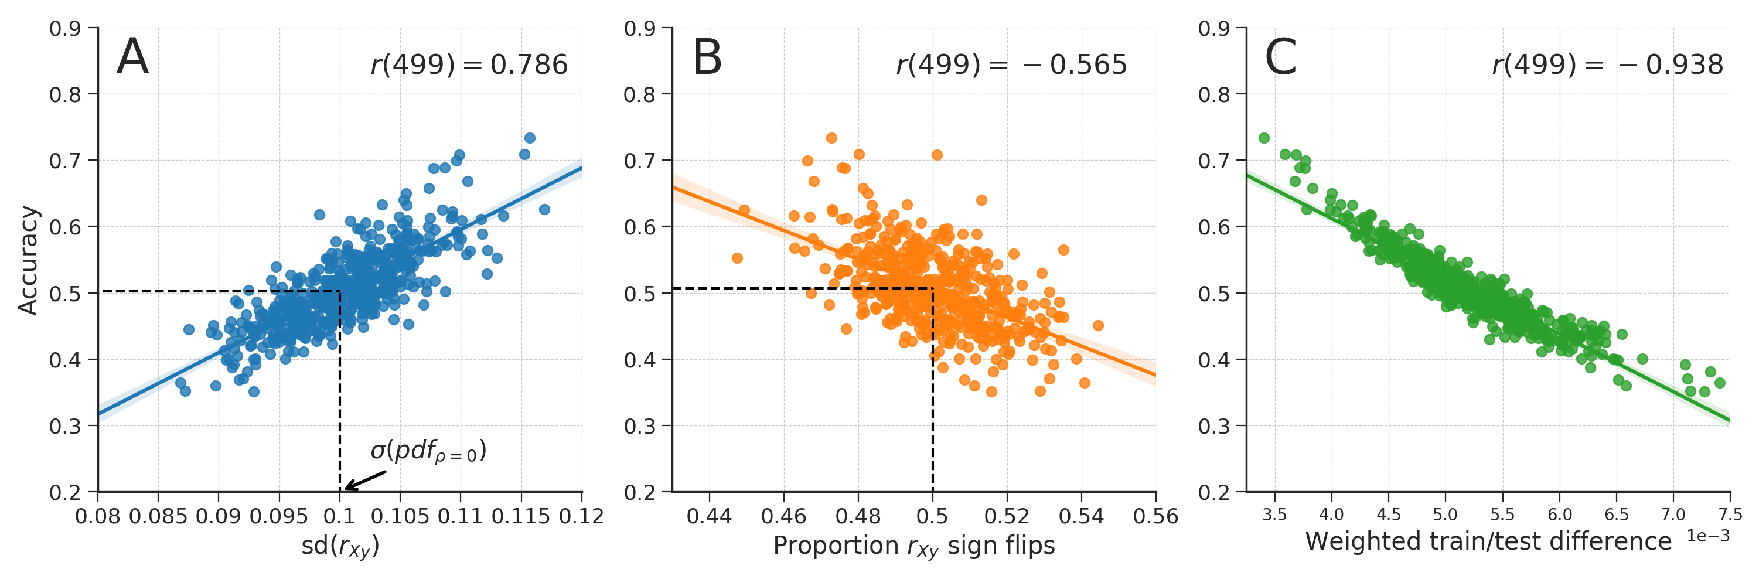
\includegraphics{_bookdown_files/confounds-decoding-files/figures/figure_13.pdf}
\caption{\label{fig:fig-confounds-decoding-13}\textbf{A}) The relationship between the standard deviation of the distribution of feature-target correlations, \emph{sd}(\(r_{yX}\)), and accuracy across iterations of cross-validated classification analyses of null data. The vertical dashed line represents the standard deviation from the sampling distribution parameterized with \(\rho = 0\) and \(N = 100\) (i.e., the same parameters used to generate the null data); the horizontal dashed line represents the expected accuracy for data with this standard deviation based on the regression line estimated from the data across simulations (see Supplementary Figure \ref{fig:fig-confounds-decoding-S15} for the same plot with different values for \(N\)). \textbf{B}) The relationship between the proportion of features of which the sign of their correlation with the target (\(r_{Xy}\)) ``flips'' between the train-set and the test-set and accuracy. The vertical dashed line represents a proportion of 0.5., i.e., 50\% of the features flip their correlation sign, which corresponds approximately with an accuracy of 0.5. \textbf{C}) The relationship between the weighted difference between feature-target correlations in the train and test set (see equation \eqref{eq:dataset-shift}) and accuracy.}
\end{figure}



This observation, then, begs the question: \emph{why} do narrower-than-chance correlation distributions lead to below chance accuracy? One potential explanation of below chance accuracy is that the classifier may learn a particular (linear) relationship between features and the target in the train set (e.g., \(r_{Xy} = 0.05\)), while the sign of this relationship is ``flipped'' in the test set (e.g., \(r_{Xy} = -0.03\); see Jamalabadi et al., \protect\hyperlink{ref-Jamalabadi2016-gr}{2016}), which is known in the machine learning literature as ``dataset shift'' (Quionero-Candela et al., \protect\hyperlink{ref-Quionero-Candela2009-ge}{2009}). This situation would lead classifiers to predict the exact opposite classes for samples in the test set, leading to below chance accuracy. In the results of our simulated data, the standard deviation of the feature-target distribution was indeed significantly negatively correlated with the proportion of features that flipped the sign of their correlation between the train set and test set, \(r(499) = -.687\), \(p < 0.001\). This means that a higher density of feature-target correlations around 0 (i.e., a narrower width of the corresponding distribution) leads to more ``sign flips''. This phenomenon of ``sign flipping'' has been reported before in the context of (a priori) counterbalancing of categorical variables (\(X\)) with respect to the target (\(y\)), where it was observed that complete counterbalancing led to consistent ``sign flipping'' and consequently 0\% accuracy (Görgen et al., \protect\hyperlink{ref-Gorgen2017-sy}{2017}). Similarly, we found that the proportion of features that flip sign was significantly negatively correlated with accuracy, \(r = -.565\), \(p < 0.001\), indicating that larger proportions of features that flip sign leads to lower accuracy (see Figure \ref{fig:fig-confounds-decoding-13}B). Interestingly, at a proportion of 0.5, accuracy is approximately at chance level (0.5; dashed lines in Figure \ref{fig:fig-confounds-decoding-13}B).

This relationship between ``sign flipping'' and accuracy, however, leaves room for improvement in terms of explaining the variance of accuracy scores. Therefore, we sought to further refine our ``model'' of accuracy by defining dataset shift not by the proportion of sign flips, but by the average \emph{difference} between the feature-target correlations between the train set and test set. Moreover, because not all features contribute equally strongly to a classifier's prediction (i.e., they are weighted), we furthermore weighed each feature's ``shift'' by the associated classifier weight (\(w_{j}\)). Formally, we estimated dataset shift (\(\hat{ds}\)) thus as follows:

\begin{equation}
\hat{ds} = \frac{1}{K}\sum_{j=1}^{K}(r_{X_{j,\mathrm{train}},y_\mathrm{train}} - r_{X_{j,\mathrm{test}},y_\mathrm{test}})w_{j}
\label{eq:dataset-shift}
\end{equation}

Indeed, the correlation between this particular operationalization of ``dataset shift'' and accuracy across simulations was much higher than just the proportion of sign flips, \(r(499) = −0.934\) (Figure \ref{fig:fig-confounds-decoding-13}B).

Having established the relation between the standard deviation of the initial feature-target correlation distribution and accuracy, we followed up our simulation by investigating specifically the effect of WDCR on the standard deviation of the correlation distribution. We investigated this by simulating data with different strengths of the correlation between the confound and the target (\(r_{Cy}\)) and the number of features (\(K\)). From Figure \ref{fig:fig-confounds-decoding-14}A, it is clear that, while the expected chance level is 0.5 in all cases, model performance quickly drops below chance for increasing correlations between the target and the confound, as well as for increasing numbers of features; even leading to a model performance of 0\% when the confound is perfectly correlated with the target and when using 1000 features. Figure \ref{fig:fig-confounds-decoding-14}C shows that, indeed, higher values lead to narrower correlation distributions, which is shown in Figure \ref{fig:fig-confounds-decoding-14}D to yield relatively lower accuracy scores.

\begin{figure}
\centering
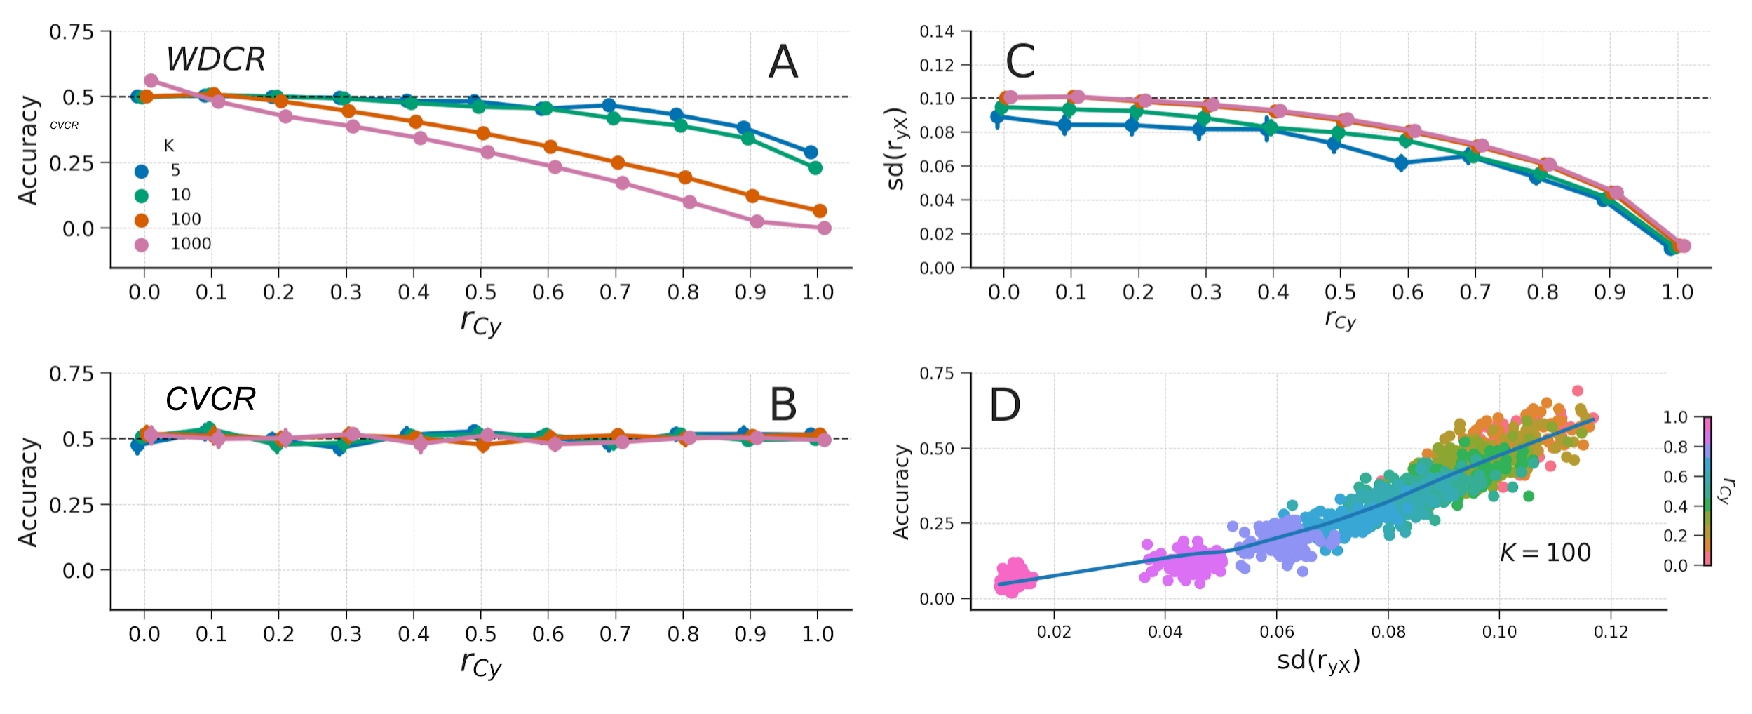
\includegraphics{_bookdown_files/confounds-decoding-files/figures/figure_14.pdf}
\caption{\label{fig:fig-confounds-decoding-14}\textbf{A}) The effect of WDCR on data varying in the correlation of the confound with the target (\(r_{Cy}\); x-axis) and the number of features (\(K\); different lines). \textbf{B}) The effect of CVCR on data varying in the correlation of the confound with the target and the number of features. The dashed black line represents chance model performance in subplots A and B. \textbf{C}) The relation between the correlation of the confound with the target (\(r_{Cy}\)) and the standard deviation of the feature-target correlation distribution, \emph{sd}(\(r_{yX}\)) for the WDCR data. The dashed black line represents the standard deviation of the correlation distribution predicted by the sampling distribution. \textbf{D}) The relation of the standard deviation of the correlation distribution and accuracy for the WDCR data (only shown for the data when \(K = 100\); see Supplementary Figure \ref{fig:fig-confounds-decoding-S18} for visualizations of this effect for different values of \(K\)). The data depicted in all panels are null data.}
\end{figure}



In summary, our simulations show that below chance accuracy is accurately predicted by the standard deviation (i.e., ``width'') of the distribution of empirical feature-target correlations and that WDCR reduces this standard deviation, which explains why the empirical analyses yielded below chance model performance (especially for larger numbers of voxels).

\hypertarget{cross-validated-confound-regression-cvcr}{%
\subsection{Cross-validated confound regression (CVCR)}\label{cross-validated-confound-regression-cvcr}}

\hypertarget{empirical-results-2}{%
\subsubsection{Empirical results}\label{empirical-results-2}}

As the results from the empirical analyses and simulations suggest, the use of WDCR is problematic because of the partitioning of the dataset into a separate train set and test set after confound regression. As such, our proposed cross-validated confound regression (CVCR) methods suggests to move the confound regression procedure inside the cross-validation loop, thereby also cross-validating this step. As expected, compared to the baseline model (i.e., no confound control), the results from the empirical analyses using CVCR show reduced (but not below chance) model performance for both VBM and TBSS data, and all different numbers of voxels (see Figure \ref{fig:fig-confounds-decoding-15}). Notably, for some numbers of voxels, model performance was not significantly above chance level.

\begin{figure}
\centering
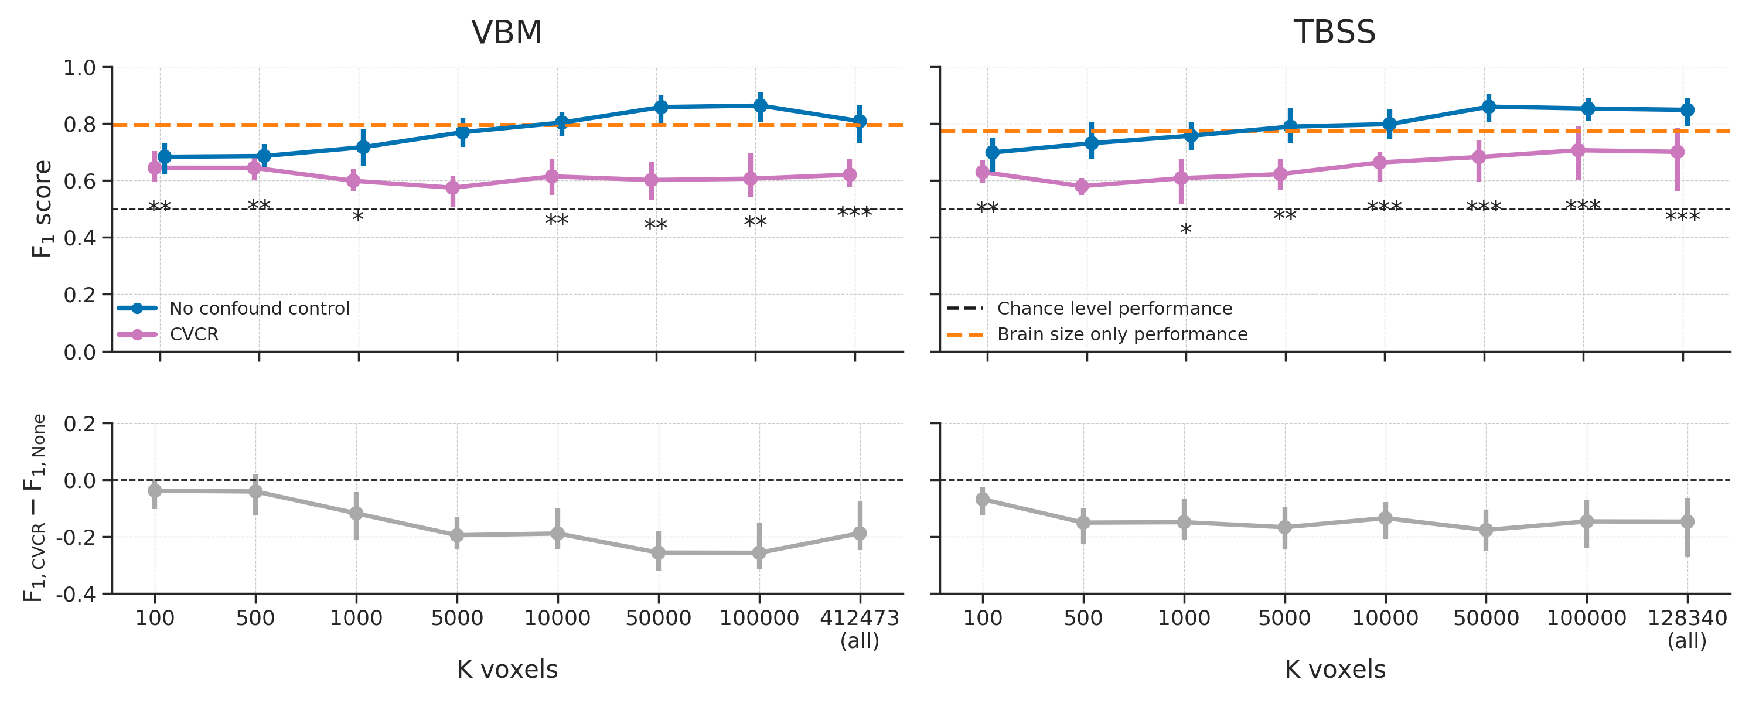
\includegraphics{_bookdown_files/confounds-decoding-files/figures/figure_15.pdf}
\caption{\label{fig:fig-confounds-decoding-15}Model performance after CVCR (pink) versus the baseline performance (blue) for both the VBM (left) and TBSS (right) data. Performance reflects the average \(F_{1}\) score across 10 folds; error bars reflect 95\% confidence intervals across 1000 bootstrap replications. The dashed black line reflect theoretical chance level performance (0.5) and the dashed orange line reflects the average model performance when only brain size is used as a predictor. Asterisks indicates performance of the CVCR model that is significantly above or below chance: *** = \(p < 0.001\), ** = \(p < 0.01\), * = \(p < 0.05\).}
\end{figure}



We also evaluated whether regressing the confound from the train set only was sufficient to control for confounds, but found that it does not effectively control for confounds when there is no true signal (i.e., there is positive bias), which is visualized in more detail in Supplementary Figure \ref{fig:fig-confounds-decoding-S10} (cf.~Figure \ref{fig:fig-confounds-decoding-8}).

\hypertarget{efficacy-analysis-1}{%
\subsubsection{Efficacy analysis}\label{efficacy-analysis-1}}

Similar to WDCR, CVCR yielded plausible and unbiased model performance (see Figure \ref{fig:fig-confounds-decoding-8}, pink line). Moreover, when applied to the simulated null data, CVCR yielded model performance scores at chance level across all levels of the confound-target correlation and numbers of features (see Figure \ref{fig:fig-confounds-decoding-14}B).

\hypertarget{summary-methods-for-confound-control}{%
\subsection{Summary methods for confound control}\label{summary-methods-for-confound-control}}

In this section, we investigated the effects of different method to control confounds (post hoc counterbalancing, WDCR, and CVCR) on empirical MRI data and simulated data (see Figure \ref{fig:fig-confounds-decoding-16} for a summary of the empirical results). Post hoc counterbalancing was, at least using the subsampling method described, clearly unable to effectively control for confounding influences, which is putatively caused by indirect circularity in the analysis process due to subsampling. Confound regression showed an expected drop in model performance (but not below chance level), but only when the confound regression step is properly cross-validated (i.e., the CVCR version).

\begin{figure}
\centering
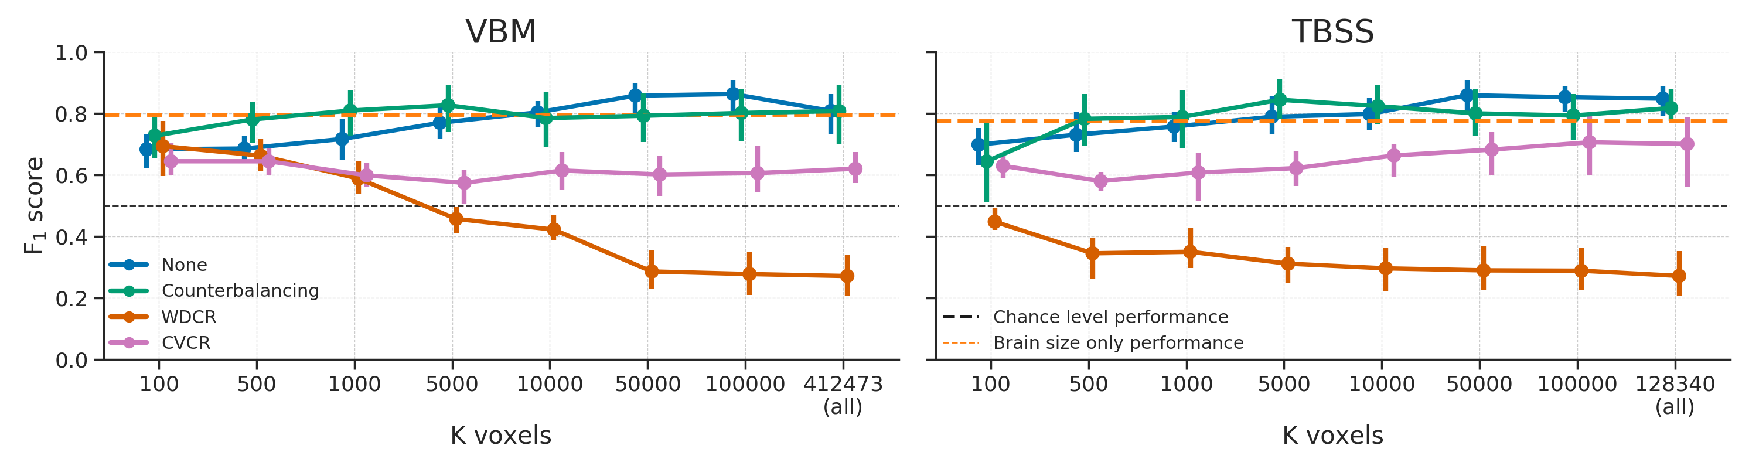
\includegraphics{_bookdown_files/confounds-decoding-files/figures/figure_16.pdf}
\caption{\label{fig:fig-confounds-decoding-16}An overview of the empirical results on the four different confound methods: None, post hoc counterbalancing, WDCR, and CVCR.}
\end{figure}



\hypertarget{confounds-decoding-discussion}{%
\section{Discussion}\label{confounds-decoding-discussion}}

Decoding analyses have become a popular alternative to univariate analyses of neuroimaging data. This analysis approach, however, inherently suffers from ambiguity in terms of which source of information is picked up by the decoder (Naselaris \& Kay, \protect\hyperlink{ref-Naselaris2015-jn}{2015}). Given that one is often interested in model interpretability rather than merely accurate prediction (Hebart \& Baker, \protect\hyperlink{ref-Hebart2017-jn}{2017}), one should strive to control for alternative sources of information (i.e., other than the target of interest) that might drive decoding. Effectively controlling for these alternative sources of information, or \emph{confounds}, helps in disambiguating decoding models. In this article, we reviewed and tested two generic, broadly applicable methods that aim to control for confounds in decoding analyses: post hoc counterbalancing and confound regression. Additionally, we proposed a third method that, unlike the other two methods, has shown to effectively control for confounds.

Both when applied to empirical and simulated data, we found that neither post hoc counterbalancing nor (whole-dataset) confound regression yielded plausible and unbiased model performance estimates. First, we found that post hoc counterbalancing leads to \emph{optimistic} (i.e., positively biased) model performance estimates, which is a result of removing samples that are hard to classify or would be wrongly classified, during the subsampling process. Because this subsampling process is applied to the entire dataset at once (i.e., it is not cross-validated), it can be seen as a form of indirect circular analysis (Kriegeskorte et al., \protect\hyperlink{ref-kriegeskorte2009circular}{2009}), in which the data themselves are used to inform analysis decisions, which can lead to biased generalization estimates. Second, our initial evaluation of confound regression, which was applied on the entire dataset (``WDCR''), yielded pessimistic (i.e., negatively biased) and even significantly below chance model performance estimates. Extending previous research (Jamalabadi et al., \protect\hyperlink{ref-Jamalabadi2016-gr}{2016}), we show that this negative bias occurs when the ``signal'' in the data (operationalized as the width of the feature-target correlation distribution) is lower than would be expected by chance, which we link to the sampling distribution of the Pearson correlation coefficient. Importantly, we show that WDCR systematically narrows the width of the correlation distribution --- and thus leads to lower model performance --- which is exacerbated by both higher correlations between target and confound, as well as by a larger number of features.

The negative bias observed in WDCR is caused by the fact that it is performed on the whole dataset at once, leading to statistical dependencies between subsequent train and test partitions. To overcome this negative bias, we propose to cross-validate the confound regression procedure (which we call ``Cross-Validated Confound Regression'', CVCR). We show that this method yields plausible model performance in the empirical analyses (i.e., significantly above chance model performance) and nearly unbiased model performance in the simulations, for different datasets varying in the amount of features (\(K\)) and the strength of the confound (\(r_{Cy}\)). Moreover, initial supplementary simulations suggest that these results generalize to (simulated) fMRI data (Supplementary Figure \ref{fig:fig-confounds-decoding-S1}), seemingly demonstrating effective control of confounds across different degrees of autocorrelation (Supplementary Figure \ref{fig:fig-confounds-decoding-S2}). The method may show some negative bias in some scenarios due to the fact that, in the train set, CVCR will remove all variance associated with the confound (even variance \emph{spuriously} correlated with the confound). However, this bias seems, at least in the simulated scenarios, very small. Overall, we believe that our results demonstrate that CVCR is a flexible and effective method to control for confounds in decoding analyses of neuroimaging data.

\hypertarget{relevance-and-consequences-for-previous-and-future-research}{%
\subsection{Relevance and consequences for previous and future research}\label{relevance-and-consequences-for-previous-and-future-research}}

\hypertarget{a-priori-and-post-hoc-counterbalancing}{%
\subsubsection{A priori and post hoc counterbalancing}\label{a-priori-and-post-hoc-counterbalancing}}

We believe our results have implications not only for post hoc counterbalancing, but a priori counterbalancing in observational designs in general. In both behavioral research (Wacholder et al., \protect\hyperlink{ref-Wacholder1992-wb}{1992}) and neuroimaging research (Görgen et al., \protect\hyperlink{ref-Gorgen2017-sy}{2017}), a priori counterbalancing (or case-control ``matching'') is a common strategy to avoid effects of confounds. However, as we show in the current study, this may unintentionally remove samples that are harder to predict, especially when there is little shared variance between the confound and the other predictors (i.e., when there is low confound \(R^2\)). Because, conceptually, this represents a form of circular analysis, counterbalancing --- regardless of whether it is applied a priori or post hoc --- can yield biased model performance estimates. To some extent, the bias in the post hoc counterbalancing results should not come as a surprise: as noted in the \protect\hyperlink{confounds-decoding-methods}{Methods} section, counterbalancing in observational research requires the researcher to choose a sample that is not representative of the population (see also Sedgwick, \protect\hyperlink{ref-Sedgwick2013-op}{2013}). As a result, out-of-sample predictive performance drops significantly, in our case even to chance level.

Since post hoc counterbalancing does not show any positive bias in model performance when there is no signal at all (i.e., signal \(R^2\)), one could argue that any observed significant above chance effect, while positively biased in terms of effect magnitude, can be interpreted as evidence that there must be signal in the data in the first place. However, we argue against this interpretation for two reasons. First, any above chance predictive performance of models fitted after subsampling is not only positively biased, but also does not cross-validate to the rejected samples (see Figure \ref{fig:fig-confounds-decoding-11}). That is, the model picks up relations between features and target that are only present in the subsample, and not in the samples left out of the analysis. As a result, it is questionable whether (and if so, how) the model should be interpreted --- after all, we assume that the rejected samples were drawn from the population of interest in a valid way. Second, any possible absence of above chance model performance after subsampling can neither be interpreted as evidence for an \emph{absence} of a true effect, since the subsampling procedure necessarily leads to a (often substantial) power loss. It could still well be that in the original sample there was a true relation between features and target. Thus, interpretation of modelling efforts after subsampling is problematic in case of both \emph{presence} and \emph{absence} of above chance model performances.

\hypertarget{confound-regression-1}{%
\subsubsection{Confound regression}\label{confound-regression-1}}

In contrast to post hoc counterbalancing, confound regression in its uncross-validated form (i.e., WDCR) has been applied widely in the context of decoding analyses (Dubois et al., \protect\hyperlink{ref-dubois2018resting}{2018}; Kostro et al., \protect\hyperlink{ref-Kostro2014-cm}{2014}; Rao et al., \protect\hyperlink{ref-Rao2017-bw}{2017}; Todd et al., \protect\hyperlink{ref-Todd2013-sd}{2013}). Indeed, the first study that systematically investigated the effect of confounds in decoding analyses (Todd et al., \protect\hyperlink{ref-Todd2013-sd}{2013}) used WDCR to account for the confounding effect of reaction times (RT) on decoding of rule representations and found that WDCR completely eliminated the predictive performance that was found without controlling for RT. This observation, however, can potentially be explained by the negative bias induced by WDCR. This possible explanation is corroborated by a follow-up study that similarly looked into RT confounding the decoding of rule representations (Woolgar et al., \protect\hyperlink{ref-Woolgar2014-jb}{2014}), who did not use WDCR but accounted for RT confounding by including it as a covariate during the pattern estimation procedure (see \protect\hyperlink{confounds-decoding-supplement}{Supplementary Materials} for a tentative evaluation of this method), which in contrast to the study by Todd et al.~yielded significant decoding performance. Moreover, while not specifically investigated here, we expect a similar negative bias to occur when a confound is removed from a continuous target variable using WDCR --- which may offer an explanation for the null finding of Dubois et al. (\protect\hyperlink{ref-dubois2018resting}{2018}), who fail to decode personality characteristics from resting-state fMRI.

\hypertarget{relevance-to-other-analysis-methods}{%
\subsubsection{Relevance to other analysis methods}\label{relevance-to-other-analysis-methods}}

While this article focuses on controlling for confounds in decoding analyses specifically, we believe that our findings may be relevant for analysis methods beyond decoding analyses as well. In fact, methods for controlling for confounds (or alternative sources of information) have previously been investigated and applied in another type of MVPA named ``representational similarity analysis'' (RSA; Kriegeskorte et al., \protect\hyperlink{ref-kriegeskorte2008representational}{2008}). In the context of RSA, the explained variance in the neural data is often partitioned into different (model-based) feature sets (i.e., sources of information), which allows one to draw conclusions about the unique influence of each source of information (see, e.g., Groen et al., \protect\hyperlink{ref-Groen2018-qo}{2018}; Hebart et al., \protect\hyperlink{ref-Hebart2018-dz}{2018}; Ramakrishnan et al., \protect\hyperlink{ref-Ramakrishnan2014-ki}{2014}). Specifically, variance partitioning in RSA is done by removing the variance from the representational dissimilarity matrix (RDM) based on the feature set that needs to be controlled for. Notably, the variance of the RDMs that are not of interest can be removed from only the neural RDM (Hebart et al., \protect\hyperlink{ref-Hebart2018-dz}{2018}; Ramakrishnan et al., \protect\hyperlink{ref-Ramakrishnan2014-ki}{2014}) or both from the neural RDM and the RDM of interest (Groen et al., \protect\hyperlink{ref-Groen2018-qo}{2018}). While the analysis context is different, the underlying technique is identical to confound regression as described and evaluated in this article. Importantly, the studies employing this variance partitioning technique (Groen et al., \protect\hyperlink{ref-Groen2018-qo}{2018}; Hebart et al., \protect\hyperlink{ref-Hebart2018-dz}{2018}; Ramakrishnan et al., \protect\hyperlink{ref-Ramakrishnan2014-ki}{2014}) similarly report plausible model performances after confound regression (i.e., relatively lower but not below chance performance), corroborating our results with (cross-validated) confound regression. Note that the distinction between WDCR and CVCR in the context of most RSA studies (including the aforementioned studies) is largely irrelevant, as representational similarity analyses are not commonly cross-validated. However, recently, some have proposed to use cross-validated distance measures (such as the cross-validated Mahalanobis distance; Guggenmos et al., \protect\hyperlink{ref-Guggenmos2018-rr}{2018}; Walther et al., \protect\hyperlink{ref-Walther2016-je}{2016}) in RSA, which could suffer from negative bias when combined with (not cross-validated) variance partitioning similar to what we observed with WDCR in the context of decoding analyses.

We believe that especially our findings with regard to WDCR and CVCR may be relevant for any cross-validated analysis, regardless of the ``direction'' of analysis (encoding vs.~decoding) and the dimensionality of the neural data (univariate vs.~multivariate approaches). In general, our findings with respect to negative bias after WDCR were to be expected, as it introduces dependence between the train set and the test set which violates the crucial assumption of independence of any cross-validated analysis. While a violation of the independence assumption often leads to positive bias such as in ``double dipping'' (Kriegeskorte et al., \protect\hyperlink{ref-kriegeskorte2009circular}{2009}), we show here that it may also lead to negative bias. Either way, our findings reinforce the idea that data analysis operations should \emph{never} be applied to the entire dataset before subjecting the data to a cross-validated analysis. Therefore, we believe that our findings with respect to WDCR and CVCR will generalize to any cross-validated analysis (such as cross-validated MANOVA, Allefeld \& Haynes, \protect\hyperlink{ref-allefeld2014searchlight}{2014}; or cross-validated encoding models, Naselaris et al., \protect\hyperlink{ref-Naselaris2011-oh}{2011}), but future research is necessary to substantiate this claim.

\hypertarget{importance-for-gender-decoding-studies}{%
\subsubsection{Importance for gender decoding studies}\label{importance-for-gender-decoding-studies}}

The importance of proper confound control is moreover highlighted by the empirical question we address. Without any optimization of the prediction pipeline, we were able to predict gender with a model performance up to approximately 0.85 without confound control. This is in line with reports from various other studies (Del Giudice et al., \protect\hyperlink{ref-Del_Giudice2016-ns}{2016}; Rosenblatt, \protect\hyperlink{ref-Rosenblatt2016-oy}{2016}; Sepehrband et al., \protect\hyperlink{ref-Sepehrband2018-dy}{2018}). However, this predictive performance is driven by a mixture two sources of information: global and local differences in brain structure. With confound control, however, we show that predictive performance using only local differences lies around 0.6 for VBM data and 0.7 for TBSS data --- a substantial drop in performance. Especially because the remaining predictive performance is lower than predictive performance using only brain size, we argue that the use of proper confound control may lead one to draw substantially different conclusions about the differences in brain structure between men and women. For the debate on gender dimorphism, it is thus extremely important to take global brain size into account in the context of decoding analyses (as has been similarly recommended for mass-univariate analyses; Barnes et al., \protect\hyperlink{ref-Barnes2010-pu}{2010}).

\hypertarget{choosing-a-confound-model-linear-vs.-nonlinear-models}{%
\subsection{Choosing a confound model: linear vs.~nonlinear models}\label{choosing-a-confound-model-linear-vs.-nonlinear-models}}

In the present paper, we focused on the use of linear models for confound control. It is crucial to note that the efficacy of confound control depends on the suitability of the confound regression model employed. Removing variance associated with a confound using a linear model removes only the variance of data (features) that is linearly related to the confound. When a confound is nonlinearly related to the data, some variance associated with the confound can remain in the data after a linear confound model is used to regress out variance. It is possible that the decoding model subsequently applied still picks up this residual ``confounded'' variance. In other words, an unsuitable confound model may control for confounds imperfectly.

The exact relation between confound and (brain) data is hardly ever known a priori. However, it is possible to explore the nature of this relation using the data at hand. For example, a researcher can apply a cross-validated prediction pipeline to predict a feature (e.g., VBM voxel intensity) from the confound. The researcher can then test what type of model (linear or nonlinear) describes the relation between confound and data best. In the \protect\hyperlink{confounds-decoding-supplement}{Supplementary Materials} (section ``Linear vs nonlinear confound models: predicting VBM and TBSS data based on brain size''), we provide an example of this approach. We used linear, quadratic, and cubic regression models to predict VBM and TBSS voxel intensity using brain size as feature. In the Supplementary Results, we show that linear models perform equally well as or better than polynomial models for the majority of voxels (Supplementary Figures \ref{fig:fig-confounds-decoding-S7} and \ref{fig:fig-confounds-decoding-S9}). Further, for voxels where polynomials outperform linear models, the difference between model performances is minimal (Supplementary Figure \ref{fig:fig-confounds-decoding-S8}). Thus, in the empirical research question explored in this paper, a linear confound model seems to suit the data very well.

\hypertarget{practical-recommendations}{%
\subsection{Practical recommendations}\label{practical-recommendations}}

As indicated by the title of this article, we will now outline some practical recommendations for dealing with confounds in decoding analyses of neuroimaging data. First, one needs to obtain an accurate measurement of potential confounds (Westfall \& Yarkoni, \protect\hyperlink{ref-westfall2016statistically}{2016}). While we assumed the availability of such a measure in this article, this is not always trivial. In experimental settings, for example, reaction times can potentially be identified as a confound (Todd et al., \protect\hyperlink{ref-Todd2013-sd}{2013}; Woolgar et al., \protect\hyperlink{ref-Woolgar2014-jb}{2014}), but arguably, it is not reaction time but rather an unobserved variable related to reaction time (e.g., difficulty or attention) that confounds the analysis. In such scenarios, the best one can do is measure reaction time as a proxy, and be aware that any subsequent confound control method is limited by how well this proxy corresponds to the actual confound. Second, one needs to identify which variables actually confound a decoding analysis. To detect confounds, we recommend using the ``same analysis approach'' outlined by Görgen et al. (\protect\hyperlink{ref-Gorgen2017-sy}{2017}). In short, this method involves trying to predict the target variable using your confound(s) as predictive features (for example, when using only brain size to predict gender). In case of significant above chance decoding performance, and assuming the confounds are actually encoded in the neuroimaging data, the hypothesized confounds will most likely influence the actual decoding analysis. While in the current article we focused on simple univariate confounding effects (i.e., confounding by a single variable), the same analysis approach is not limited to detecting univariate confounds --- it facilitates detecting multivariate (i.e., confounding by multiple variables) or interaction effects (i.e., confounding by interaction effects between variables) as well. For example, if one hypothesizes that the target variable is related to the interaction between confound \(C_{1}\) and \(C_{2}\) (i.e., \(C_{1} \times C_{2}\)), one can simply use the interaction term as the potential confound in the same analysis approach to evaluate the potential confounding influence.

Once the specific confound terms have been identified, we recommend regressing out the confound from the data in a cross-validated manner (i.e., using CVCR). Specifically, we recommend including confound regression as the first step in your decoding pipeline to avoid the effect of confounds on other operations in the pipeline (such as univariate feature selection; Chu et al., \protect\hyperlink{ref-chu2012does}{2012}). In this article, we used ordinary least squares (OLS) regression to remove the influence of confounds from the data, because a linear model describes the relation between brain size and VBM/TBSS voxel intensities well (see Supplementary Figures \ref{fig:fig-confounds-decoding-S7}-\ref{fig:fig-confounds-decoding-S9}). However, not only linear models can be used to remove variance associated with a confound from the data --- it is possible to use nonlinear models (potentially with multiple confounds and interactions between them) if it is clear that the relation between confounds and neuroimaging features is nonlinear (see previous section for details on choosing a confound model). However, as a limitation to the presented results, we did not test whether CVCR also leads to (nearly) unbiased results when used with nonlinear models. We advise, therefore, in such cases, to first test in a simulation study whether CVCR provides an unbiased confound control method with nonlinear models before use with actual data.

\hypertarget{conclusion}{%
\section{Conclusion}\label{conclusion}}

In general, we believe that the contributions of the current study are twofold. First and foremost, it provides a systematic evaluation of widely applicable methods to control for confounds and shows that, of the methods investigated, only one (``cross-validated confound regression'') appears to yield plausible and almost unbiased results. The results from this evaluation hopefully prevents researchers from using post hoc counterbalancing and whole-dataset confound regression, which we show may introduce (unintended) biases. Moreover, we made all analyses and preprocessed data openly available (\url{https://github.com/lukassnoek/MVCA}) and provide a simple implementation for cross-validated confound regression that interfaces with the popular scikit-learn package in the Python programming language. Second, we believe that this study improves understanding of the elusive phenomenon of below chance accuracy (building on previous work by Jamalabadi et al., \protect\hyperlink{ref-Jamalabadi2016-gr}{2016}). In general, we hope that this study helps researchers in gaining more insight into their decoding analyses by providing a method that disentangles the contributions of different sources of information that may be encoded in their data.

\hypertarget{aomic}{%
\chapter{The Amsterdam Open MRI Collection, a set of multimodal MRI datasets for individual difference analyses}\label{aomic}}

\chaptermark{AOMIC}

\vspace*{\fill}

\begin{center}\rule{0.5\linewidth}{0.5pt}\end{center}

\small

\noindent
\emph{This chapter has been published as}: Snoek, L., van der Miesen, M.M., Beemsterboer, T., van der Leij, A., Eigenhuis, A., \& Scholte, H.S. (2021). The Amsterdam Open MRI Collection, a set of multimodal MRI datasets for individual difference analyses. \emph{Nature Scientific Data, 8}, 85.

\newpage
\normalsize

\begin{abstract}
We present the Amsterdam Open MRI Collection (AOMIC): three datasets with multimodal (3T) MRI data including structural (T1-weighted), diffusion-weighted, and (resting-state and task-based) functional BOLD MRI data, as well as detailed demographics and psychometric variables from a large set of healthy participants (\emph{N} = 928, \emph{N} = 226, and \emph{N} = 216). Notably, task-based fMRI was collected during various robust paradigms (targeting naturalistic vision, emotion perception, working memory, face perception, cognitive conflict and control, and response inhibition) for which extensively annotated event-files are available. For each dataset and data modality, we provide the data in both raw and preprocessed form (both compliant with the Brain Imaging Data Structure), which were subjected to extensive (automated and manual) quality control. All data is publicly available from the OpenNeuro data sharing platform.
\end{abstract} \newpage

\hypertarget{background-summary}{%
\section{Background \& summary}\label{background-summary}}

It is becoming increasingly clear that robust effects in neuroimaging studies require very large sample sizes (Button et al., \protect\hyperlink{ref-Button2013-zu}{2013}; Yarkoni, \protect\hyperlink{ref-Yarkoni2009-pz}{2009}), especially when investigating between-subject effects (Dubois \& Adolphs, \protect\hyperlink{ref-Dubois2016-zz}{2016}). With this in mind, we have run several large-scale ``population imaging'' MRI projects over the past decade at the University of Amsterdam, with the aim to reliably estimate the (absence) of structural and functional correlates of human behavior and mental processes. After publishing several articles using these datasets (Elk \& Snoek, \protect\hyperlink{ref-Van_Elk2020-xo}{2020}; Hoogeveen et al., \protect\hyperlink{ref-Hoogeveen2020-qp}{2020}; Koolschijn et al., \protect\hyperlink{ref-Koolschijn2015-hd}{2015}; Ramakrishnan et al., \protect\hyperlink{ref-Ramakrishnan2014-ki}{2014}; Snoek et al., \protect\hyperlink{ref-Snoek2019-my}{2019}), we believe that making the data from these projects publicly available will benefit the neuroimaging community most. To this end, we present the Amsterdam Open MRI Collection (AOMIC) --- three large-scale datasets with high-quality, multimodal 3T MRI data and detailed demographic and psychometric data, which are publicly available from the OpenNeuro data sharing platform. In this article, we describe the characteristics and contents of these three datasets in a manner that complies with the guidelines of the COBIDAS MRI reporting framework (Nichols et al., \protect\hyperlink{ref-Nichols2017-ze}{2017}).

We believe that AOMIC represents a useful contribution to the growing collection of publicly available population imaging MRI datasets (Babayan et al., \protect\hyperlink{ref-Babayan2019-mo}{2019}; Mendes et al., \protect\hyperlink{ref-Mendes2019-yh}{2019}; Miller et al., \protect\hyperlink{ref-Miller2016-oi}{2016}; Van Essen et al., \protect\hyperlink{ref-Van_Essen2013-df}{2013}). AOMIC contains a large representative dataset of the general population, ``ID1000'' (\emph{N} = 928), and two large datasets with data from university students, ``PIOP1'' (\emph{N} = 216) and ``PIOP2'' (\emph{N} = 226; \emph{P}opulation \emph{I}maging \emph{o}f \emph{P}sychology). Each dataset contains MRI data from multiple modalities (structural, diffusion, and functional MRI), concurrently measured physiological (respiratory and cardiac) data, and a variety of well-annotated demographics (age, sex, handedness, educational level, etc.), psychometric measures (intelligence, personality), and behavioral information related to the task-based fMRI runs (see Figure \ref{fig:fig-aomic-1} and Table \ref{tab:tab-aomic-1} for an overview). Furthermore, AOMIC offers, in addition to the raw data, also preprocessed data from well-established preprocessing and quality control pipelines, all consistently formatted according to the Brain Imaging Data Structure (Gorgolewski et al., \protect\hyperlink{ref-Gorgolewski2016-in}{2016}). As such, researchers can quickly and easily prototype and implement novel secondary analyses without having to worry about quality control and preprocessing themselves.

Due to the size and variety of the data in AOMIC, there are many ways in which it can be used for secondary analysis. One promising direction is to use the data for the development of generative and discriminative machine learning-based algorithms, which often need large datasets to train models on. Another, but related, use of AOMIC's data is to use it as a validation dataset (rather than train-set) for already developed (machine learning) algorithms to assess the algorithm's ability to generalize to different acquisition sites or protocols. Lastly, due to the rich set of confound variables shipped with each dataset (including physiology-derived noise regressors), AOMIC can be used to develop, test, or validate (novel) denoising methods.

\begin{figure}
\centering
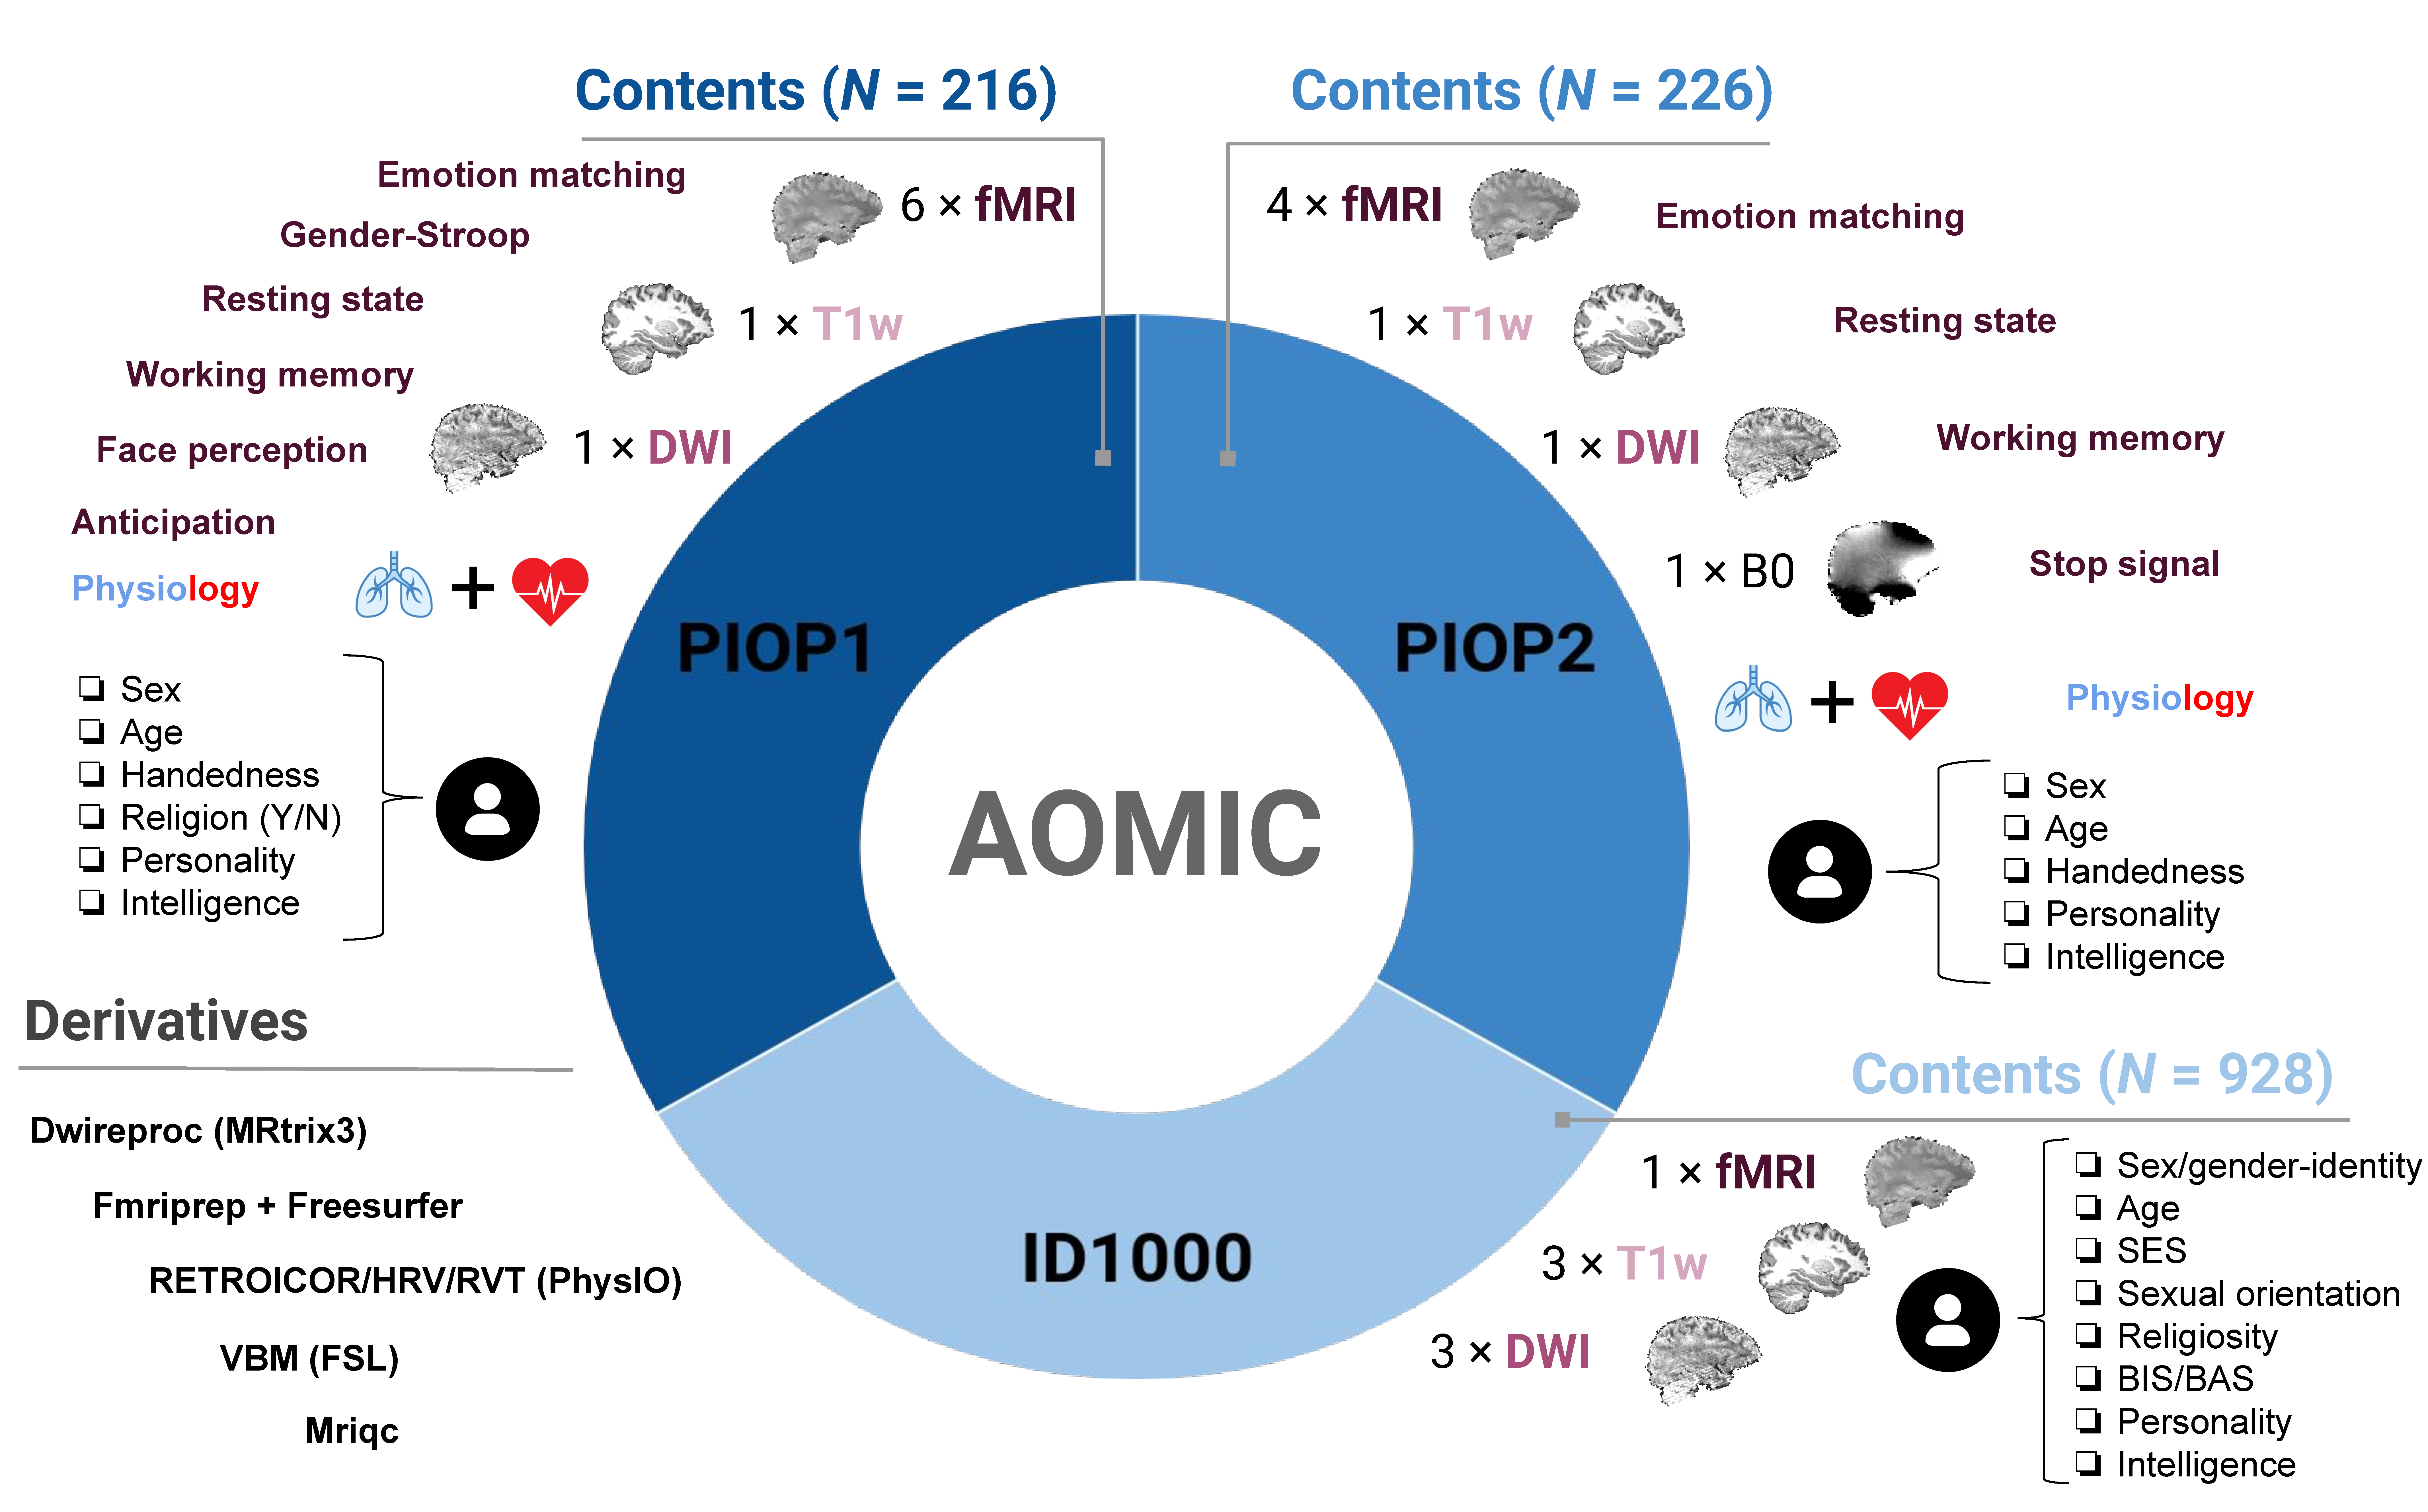
\includegraphics{_bookdown_files/aomic-files/figures/figure_1.pdf}
\caption{\label{fig:fig-aomic-1}General overview of AOMIC's contents. Each dataset (ID1000, PIOP1, PIOP2) contains multimodal MRI data, physiology (concurrent with fMRI acquisition), demographic and psychometric data, as well as a large set of ``derivatives'', i.e., data derived from the original ``raw'' data through state-of-the-art preprocessing pipelines.}
\end{figure}



\newpage
\pagestyle{empty}
\blandscape

\begingroup\fontsize{10}{12}\selectfont

\begin{ThreePartTable}
\begin{TableNotes}[para]
\item \textit{Note: } 
\item Mov: movie watching, RS: resting-state, Emo: emotion matching, G-str: gender-stroop, FP: face perception, WM: working memory, Antic: anticipation, Stop: stop-signal. Tasks without this subscript were acquired without multiband acceleration (i.e., "sequential" acquisition).
\end{TableNotes}
\begin{longtabu} to \linewidth {>{\raggedright\arraybackslash}p{5em}>{\raggedright}X>{\raggedright}X>{\raggedright}X>{\raggedright}X>{\raggedright}X>{\raggedright}X>{\raggedright}X>{\raggedright}X>{\raggedright}X>{\raggedright}X>{\raggedright}X}
\caption{\label{tab:tab-aomic-1}Overview of the number of subjects per dataset and tasks.}\\
\toprule
 & ID1000 & PIOP1 &  &  &  &  &  & PIOP2 &  &  & \\
\midrule
N subj. & 928 & 216 &  &  &  &  &  & 226 &  &  & \\
T1w & 928 & 216 &  &  &  &  &  & 226 &  &  & \\
DWI & 925 & 211 &  &  &  &  &  & 226 &  &  & \\
Fieldmap & n/a & n/a &  &  &  &  &  & 226 &  &  & \\
 &  &  &  &  &  &  &  &  &  &  & \\
\addlinespace
 & Mov & RS & Emo & G-str & FP & WM & Antic & RS & Emo & WM & Stop\\
fMRI & 881 & 210 & 208 & 208 & 203 & 207 & 203 & 214 & 222 & 224 & 226\\
Physiology & 790 & 198 & 194 & 194 & 189 & 194 & 188 & 216 & 216 & 211 & 217\\
\bottomrule
\insertTableNotes
\end{longtabu}
\end{ThreePartTable}
\endgroup{}

\elandscape
\newpage
\pagestyle{\defstyle}

\hypertarget{methods}{%
\section{Methods}\label{methods}}

In this section, we describe the details of the data acquisition for each dataset in AOMIC. We start with a common description of the MRI scanner used to collect the data. The next two sections describe the participant characteristics, data collection protocols, experimental paradigms (for functional MRI), and previous analyses separately for the ID1000 study and the PIOP studies. Then, two sections describe the recorded subject-specific variables (such as educational level, background socio-economic status, age, etc.) and psychometric measures from questionnaires and tasks (such as intelligence and personality). Finally, we describe how we standardized and preprocessed the data, yielding an extensive set of ``derivatives'' (i.e., data derived from the original raw data).

\hypertarget{scanner-details-and-general-scanning-protocol-all-datasets}{%
\subsection{Scanner details and general scanning protocol (all datasets)}\label{scanner-details-and-general-scanning-protocol-all-datasets}}

Data from all three datasets were acquired on the same Philips 3T scanner (Philips, Best, the Netherlands), but underwent several upgrades in between the three studies. The ID1000 dataset was scanned on the ``Intera'' version, after which the scanner was upgraded to the ``Achieva'' version (converting a part of the signal acquisition pathway from analog to digital) on which the PIOP1 dataset was scanned. After finishing the PIOP1 study, the scanner was upgraded to the ``Achieva dStream'' version (with even earlier digitalization of the MR signal resulting in less noise interference), on which the PIOP2 study was scanned. All studies were scanned with a 32-channel head coil (though the head coil was upgraded at the same time as the dStream upgrade). Although not part of AOMIC, a separate dataset (dStreamUpgrade) with raw and preprocessed data (DWI, T1-weighted, and both resting-state and task-based functional MRI scans) acquired before and after the dStream upgrade using the same sequences and participants in both sessions is available on OpenNeuro (K Gorgolewski et al., \protect\hyperlink{ref-Gorgolewski2017-uu}{2017}). In addition, unthresholded group-level temporal signal-to-noise ratio (tSNR) maps and group-level GLM maps (for both the pre-upgrade and post-upgrade data as well as the post-pre difference) are available on NeuroVault (Gorgolewski, Varoquaux, Rivera, Schwarz, Ghosh, Maumet, Sochat, Nichols, Poldrack, Poline, Yarkoni, et al., \protect\hyperlink{ref-Gorgolewski2015-hj}{2015}).

At the start of each scan session, a low resolution survey scan was made, which was used to determine the location of the field-of-view. For all structural (T1-weighted), fieldmap (phase-difference based B0 map), and diffusion (DWI) scans, the slice stack was not angled. This was also the case for the functional MRI scans of ID1000 and PIOP1, but for PIOP2 the slice stack for functional MRI scans was angled such that the eyes were excluded as much as possible in order to reduce signal dropout in orbitofrontal cortex. While the set of scans acquired for each study is relatively consistent (i.e., at least one T1-weighted anatomical scan, at least one diffusion-weighted scan, and at least one functional BOLD MRI scan), the parameters for a given scan vary slightly between the three studies. Notably, the functional MRI data from the resting-state and faces tasks from PIOP1 were acquired with multi-slice acceleration (factor 3; referred to in the current article as ``multiband'' acquisition), while all other functional MRI scans, including those from ID1000 and PIOP2, were acquired without multi-slice acceleration (referred to in the current article as ``sequential'' acquisition). The reason for reverting to sequential (instead of multiband) acquisition of the resting state scan in PIOP2 is that we did not think the reduction in tSNR observed in multiband scans outweighs the increase in number of volumes. In Supplementary Tables \ref{tab:tab-aomic-S1}-\ref{tab:tab-aomic-S4}, the parameters for the different types of scans across all three studies are listed.

During functional MRI scans, additional physiological data was recorded. Respiratory traces were recorded using a respiratory belt (air filled cushion) bound on top of the subject's diaphragm using a velcro band. Cardiac traces were recorded using a plethysmograph attached to the subject's left ring finger. Data was transferred to the scanner PC as plain-text files (Philips ``SCANPHYSLOG'' files) using a wireless recorder with a sampling frequency of 496 Hz.

Experimental paradigms for the functional MRI runs were shown on a 61 \(\times\) 36 cm screen using a DLP projector with a 60 Hz refresh rate (ID1000 and PIOP1) or on a Cambridge Electronics BOLDscreen 32 IPS LCD screen with a 120 Hz refresh rate (PIOP2), both placed at 113 cm distance from the mirror mounted on top of the head coil. Sound was presented via a MRConfon sound system. Experimental tasks were programmed using Neurobs Presentation (Neurobehavioral Systems Inc, Berkeley, U.S.A.) and run on a Windows computer with a dedicated graphics card. To allow subject responses in experimental tasks (PIOP1 and PIOP2 only), participants used MRI-compatible fibre optic response pads with four buttons for each hand (Cambridge Research Systems, Rochester, United Kingdom).

\hypertarget{id1000-specifics}{%
\subsection{ID1000 specifics}\label{id1000-specifics}}

In this section, we describe the subject recruitment, subject characteristics, data collection protocol, functional MRI paradigm, and previous analyses of the ID1000 study.

\hypertarget{subjects}{%
\subsubsection{Subjects}\label{subjects}}

The data from the ID1000 sample was collected between 2010 and 2012. The faculty's ethical committee approved this study before data collection started (EC number: 2010-BC-1345). Potential subjects were a priori excluded from participation if they did not pass a safety checklist with MRI contraindications. We recorded data from 992 subjects of which 928 are included in the dataset (see \protect\hyperlink{aomic-technical-validation}{Technical validation} for details on the post-hoc exclusion procedure). Subjects were recruited through a recruitment agency (Motivaction International B.V.) in an effort to get a sample that was representative of the general Dutch population in terms of educational level (as defined by the Dutch government, Onderwijsindeling, \protect\hyperlink{ref-Onderwijsindeling2016-tb}{2016}), but drawn from only a limited age range (19 to 26). We chose this limited age range to minimize the effect of aging on any brain-related covariates. A more detailed description of educational level and other demographic variables can be found in the section ``Subject variables''.

\hypertarget{data-collection-protocol}{%
\subsubsection{Data collection protocol}\label{data-collection-protocol}}

Prior to the experiment, subjects were informed about the goal and scope of the research, the MRI procedure, safety measures, general experimental procedures, privacy and data sharing concerns, and voluntary nature of the project (i.e., subjects were told that they could stop with the experiment at any time, without giving a reason for it). Before coming to the scan center, subjects also completed a questionnaire on background information (to determine educational level, which was used to draw a representative sample). If participants were invited they provided informed consent and completed an MRI screening checklist. Subjects then completed an extensive set of questionnaires and tests, including a general demographics questionnaire, the Intelligence Structure Test (Amthauer et al., \protect\hyperlink{ref-Amthauer2001-yg}{2001}; Vorst, \protect\hyperlink{ref-Vorst2010-ex}{2010}), the ``trait'' part of the State-Trait Anxiety Inventory (STAI; Spielberger et al., \protect\hyperlink{ref-Spielberger1970-td}{1970}), a behavioral avoidance/inhibition questionnaire (BIS/BAS; Carver \& White, \protect\hyperlink{ref-Carver1994-wp}{1994}; Franken et al., \protect\hyperlink{ref-Franken2005-jg}{2005}), multiple personality questionnaires --- amongst them the MPQ (Eigenhuis et al., \protect\hyperlink{ref-Eigenhuis2013-xo}{2013}) and the NEO-FFI (Hoekstra et al., \protect\hyperlink{ref-Hoekstra1996-kv}{1996}; Van der Ploeg, \protect\hyperlink{ref-Van_der_Ploeg1980-tq}{1980}) and several behavioral tasks. The psychometric variables of the tests included in the current dataset are described in the section ``Psychometric variables''.

Testing took place from 9 AM until 4 PM and on each day two subjects were tested. One subject began with the IST intelligence test, while the other subject started with the imaging part of the experiment. For the MRI part, we recorded three T1-weighted scans, three diffusion-weighted scans, and one functional (BOLD) MRI scan (in that order). The scanning session lasted approximately 60 minutes. Afterwards, the subjects switched and completed the other part. After these initial tasks, the subjects participated in additional experimental tasks, some of which have been reported in other publications (Gazendam et al., \protect\hyperlink{ref-Gazendam2015-fr}{2015}; Pinto et al., \protect\hyperlink{ref-Pinto2013-kh}{2013}) and are not included in this dataset.

\hypertarget{functional-mri-paradigm}{%
\subsubsection{Functional MRI paradigm}\label{functional-mri-paradigm}}

During functional MRI acquisition, subjects viewed a movie clip consisting of a (continuous) compilation of 22 natural scenes taken from the movie Koyaanisqatsi (Reggio, \protect\hyperlink{ref-Reggio1982-ex}{1982}) with music composed by Philip Glass. The scenes were selected because they broadly sample a set of visual parameters (textures and objects with different sizes and different rates of movement). Importantly, the focus on variation of visual parameters means, in this case, that the movie lacks a narrative and thus may be inappropriate to investigate semantic or other high-level processes.

The scenes varied in length from approximately 5 to 40 seconds with ``cross dissolve'' transitions between scenes. The movie clip extended 16 degrees visual angle (resolution 720 \(\times\) 576, movie frame rate of 25 Hz). The onset of the movie clip was triggered by the first volume of the fMRI acquisition and had a duration of 11 minutes (which is slightly longer than the fMRI scan, i.e., 10 minutes and 38 seconds). The movie clip is available in the ``stimuli'' subdirectory of the ID1000 dataset (with the filename \texttt{task-moviewatching\_desc-koyaanisqatsi\_movie.mp4}).

\hypertarget{previous-analyses}{%
\subsubsection{Previous analyses}\label{previous-analyses}}

The MRI data of ID1000 has been analyzed previously by two studies. One study (Ramakrishnan et al., \protect\hyperlink{ref-Ramakrishnan2014-ki}{2014}) analyzed the functional MRI data of a subset of 20 subjects by relating features from computational models applied to the movie data to the voxelwise time series using representational similarity analysis. Another study (Koolschijn et al., \protect\hyperlink{ref-Koolschijn2015-hd}{2015}) analyzed the relationship between autistic traits and voxel-based morphometry (VBM, derived from the T1-weighted scans) as well as fractional anisotropy (FA, derived from the DWI scans) in a subset of 508 subjects.

\hypertarget{piop1-and-piop2-specifics}{%
\subsection{PIOP1 and PIOP2 specifics}\label{piop1-and-piop2-specifics}}

In this section, we describe the subject recruitment, subject characteristics, data collection protocol, functional MRI paradigm, and previous analyses of the PIOP1 and PIOP2 studies. These two studies are described in a common section because their data collection protocols were very similar. Information provided in this section (including sample characteristics, sample procedure, data acquisition procedure and scan sequences) can be assumed to apply to both PIOP1 and PIOP2, unless explicitly stated otherwise. As such, these datasets can be used as train/test (or validation) partitions. The last subsection (``Differences between PIOP1 and PIOP2'') describes the main differences between the two PIOP datasets.

\hypertarget{subjects-1}{%
\subsubsection{Subjects}\label{subjects-1}}

Data from the PIOP1 dataset were collected between May 2015 and April 2016 and data from the PIOP2 dataset between March 2017 and July 2017. The faculty's ethical committee approved these studies before data collection started (PIOP1 EC number: 2015-EXT-4366, PIOP2 EC number: 2017-EXT-7568). Potential subjects were a priori excluded from participation if they did not pass a safety checklist with MRI contraindications. Data was recorded from 248 subjects (PIOP1) and 242 subjects (PIOP2), of which 216 (PIOP1) and 226 (PIOP2) are included in AOMIC (see \protect\hyperlink{aomic-technical-validation}{Technical validation} for details on the post-hoc exclusion procedure). Subjects from both PIOP1 and PIOP2 were all university students (from the Amsterdam University of Applied Sciences or the University of Amsterdam) recruited through the University websites, posters placed around the university grounds, and Facebook. A description of demographic and other subject-specific variables can be found in the section ``Subject variables''.

\hypertarget{data-collection-protocol-1}{%
\subsubsection{Data collection protocol}\label{data-collection-protocol-1}}

Prior to the research, subjects were informed about the goal of the study, the MRI procedure and safety, general experimental procedure, privacy and data sharing issues, and the voluntary nature of participation through an information letter. Each testing day (which took place from 8.30 AM until 1 PM), four subjects were tested. First, all subjects filled in an informed consent form and completed an MRI screening checklist. Then, two subjects started with the MRI part of the experiment, while the other two completed the demographic and psychometric questionnaires (described below) as well as several tasks that are not included in AOMIC.

The MRI session included a survey scan, followed by a T1-weighted anatomical scan. Then, several functional MRI runs (described below) and a single diffusion-weighted scan were recorded. Details about the scan parameters can be found in Supplementary Tables \ref{tab:tab-aomic-S1}-\ref{tab:tab-aomic-S4}. The scan session lasted approximately 60 minutes. The scans were always recorded in the same order. For PIOP1, this was the following: \emph{faces} (fMRI), \emph{gender-stroop} (fMRI), T1-weighted scan, \emph{emotion matching} (fMRI), \emph{resting-state} (fMRI), \emph{phase-difference} fieldmap (B0) scan, DWI scan, \emph{working memory} (fMRI), \emph{emotion anticipation} (fMRI). For PIOP2, this was the following: T1-weighted scan, \emph{working memory} (fMRI), \emph{resting-state} (fMRI), DWI scan, \emph{stop signal} (fMRI), \emph{emotion matching} (fMRI).

\hypertarget{functional-mri-paradigms}{%
\subsubsection{Functional MRI paradigms}\label{functional-mri-paradigms}}

In this section, we will describe the experimental paradigms used during fMRI acquisition. See Figure \ref{fig:fig-aomic-2} for a visual representation of each paradigm. None of the designs were optimized for efficiency, except for the emotion anticipation task (which was optimized for efficiency to estimate the effect of each condition). All paradigms during functional MRI were started and synced to the functional MRI acquisition using a transistor-transistor logic (TTL) pulse sent to the stimulus presentation computer.

\begin{figure}
\centering
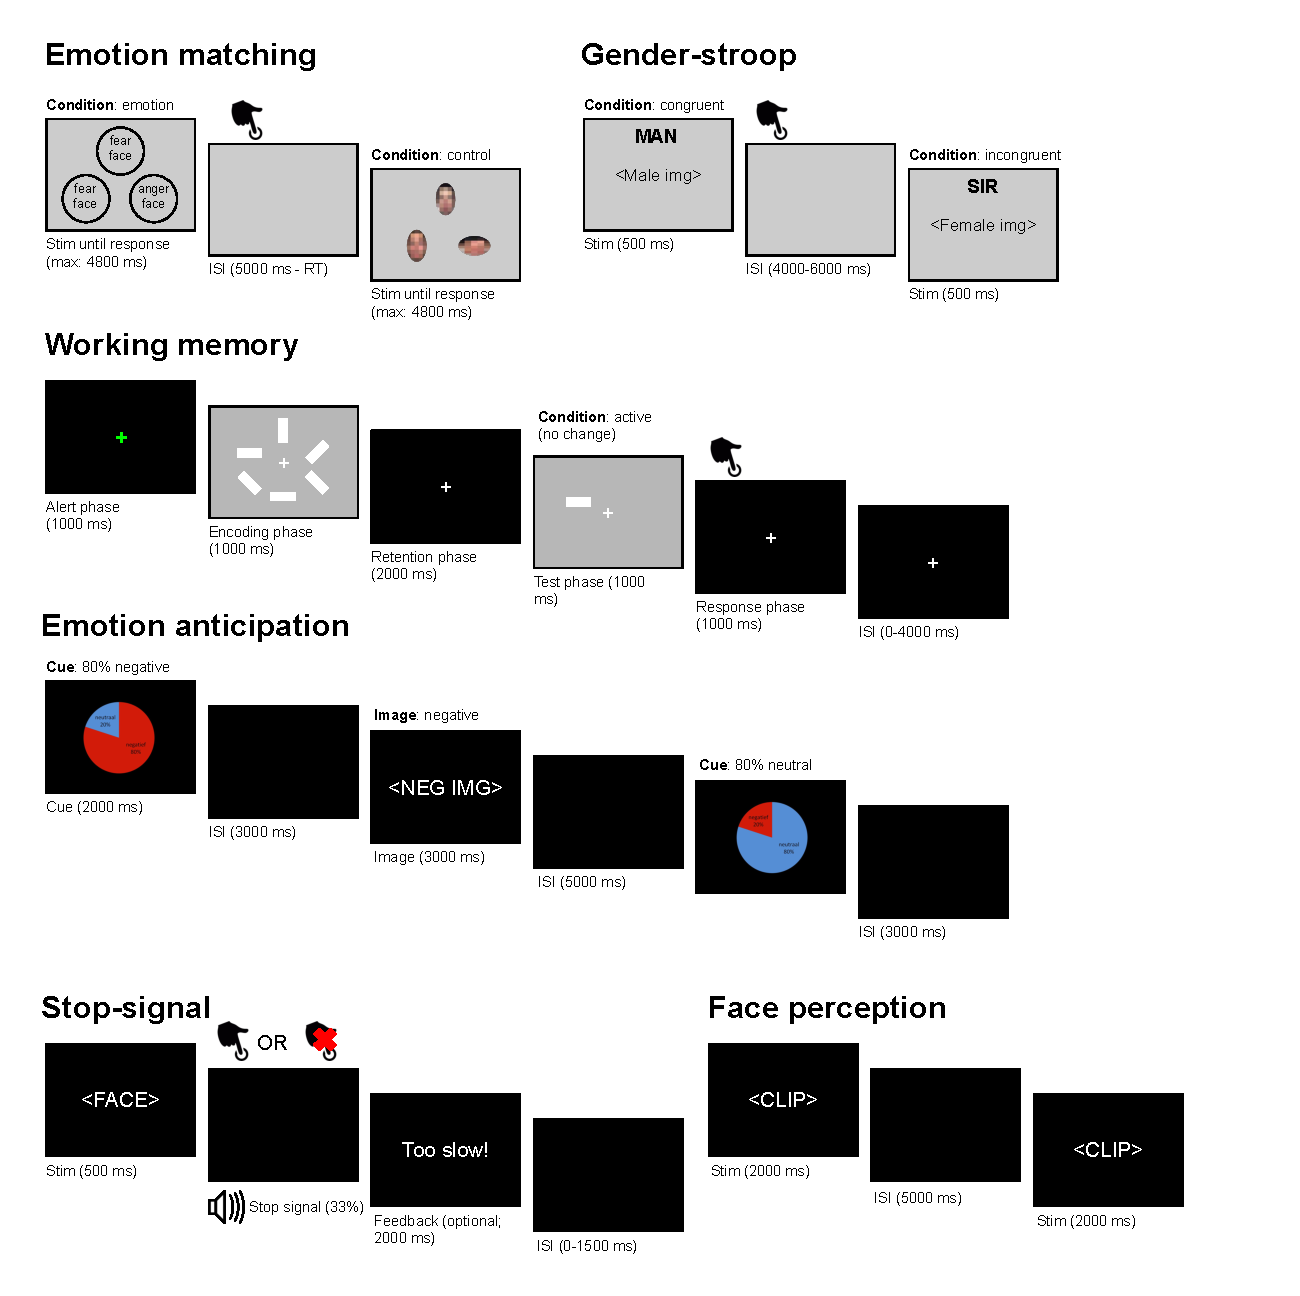
\includegraphics{_bookdown_files/aomic-files/figures/figure_2.pdf}
\caption{\label{fig:fig-aomic-2}A visual representation of all experimental paradigms during task-based fMRI. ISI: inter-stimulus interval.}
\end{figure}



\textbf{Emotion matching (PIOP1+2)}. The goal of the ``emotion matching'' task is to measure processes related to (facial) emotion processing. The paradigm we used was based on Hariri et al. (\protect\hyperlink{ref-Hariri2000-sc}{2000}). Trials were presented using a blocked design. In each trial, subjects were presented with either color images of an emotional target face (top) and two emotional probe faces (bottom left and bottom right; ``emotion'' condition) or a target oval (top) and two probe ovals (bottom left and bottom right; ``control'' condition) on top of a gray background (RGB: 248, 248, 248) and were instructed to either match the emotional expression of the target face (``emotion'' condition) or the orientation or the target oval (``control'' condition) as quickly as possible by pushing a button with the index finger of their left or right hand. The target and probes disappeared when the subject responded (or after 4.8 seconds). A new trial always appeared 5 seconds after the onset of each trial. In between the subject's response and the new trial, a blank screen was shown. Trials were presented in alternating ``control'' and ``emotion'' blocks consisting of six stimuli of 5 seconds each (four blocks each, i.e., 48 stimuli in total). Stimuli always belonged to the same block, but the order of stimuli within blocks was randomized across participants. The task took 270 seconds in total (i.e., 135 volumes with a 2 second TR).

The faces always displayed either stereotypical anger or fear. Within trials, always exactly two faces portrayed the same expression. Both male and female faces and white, black, and Asian faces were used, but within a single trial, faces were always of the same sex and ethnicity category (white or Asian/black). Face pictures were derived from the NimStim Face Stimulus set (Tottenham et al., \protect\hyperlink{ref-Tottenham2009-vn}{2009}). The oval stimuli were created by pixelating the face stimuli and were approximately the same area as the face stimuli (making them color and size matched to the face stimuli) and were either presented horizontally (i.e., the long side was horizontally aligned) or vertically (i.e., the long side was vertically aligned). Within trials, always exactly two ovals were aligned in the same way.

The fMRI ``event files'' (with the identifier *\_events*) associated with this task contain information of the trial onset (the moment the faces/ovals appeared on screen, in seconds), duration (how long the faces/ovals were presented, in seconds), trial type (either ``control'' or ``emotion''), response time (how long it took the subject to respond, logged ``n/a'' in case of no response), response hand (either ``left'', ``right'', or ``n/a'' in case of no response), response accuracy (either ``correct'', ``incorrect'', or ``miss''), orientation to match (either ``horizontal'', ``vertical'', or ``n/a'' in case of emotion trials), emotion match (either ``fear'', ``anger'', or ``n/a'' in case of control trials), gender of the faces (either ``male'', ``female'', of ``n/a'' in case of control trials), and ethnicity of the target and probe faces (either ``caucasian'', ``asian'', ``black'', or ``n/a'' in case of control trials).

\textbf{Working memory task (PIOP1+2)}. The goal of the working memory task was to measure processes related to visual working memory. The paradigm we used was based on Pessoa et al. (\protect\hyperlink{ref-Pessoa2002-tb}{2002}). Trials were presented using a fixed event-related design, in which trial order the same for each subject. Trials belonged to one of three conditions: ``active (change)'', ``active (no change)'', or ``passive''. Each trial consisted of six phases: an alert phase (1 second), an encoding phase (1 second), a retention phase (2 seconds), a test phase (1 second), a response phase (1 second), and an inter-stimulus interval (0-4 seconds). Subjects were instructed to keep focusing on the fixation target, which was shown throughout the entire trial, and completed a set of practice trials before the start of the actual task. The task took 324 seconds in total (i.e., 162 volumes with a 2 second TR).

In all trial types, trials started with an alert phase: a change of color of the fixation sign (a white plus sign changing to green, RGB {[}0, 255, 0{]}), lasting for 1 second. In the encoding phase, for ``active'' trials, an array of six white bars with a size of 2 degrees visual angle with a random orientation (either 0, 45, 90, or 135 degrees) arranged in a circle was presented for 1 second. This phase of the trial coincided with a change in background luminance from black (RGB: {[}0, 0, 0{]}) to gray (RGB: {[}120, 120, 120{]}). For ``passive'' trials, only the background luminance changed (but no bars appeared) in the encoding phase. In the subsequent retention phase, for all trial types, a fixation cross was shown and the background changed back to black, lasting 2 seconds. In the test phase, one single randomly chosen bar appeared (at one of the six locations from the encoding phase) which either matched the original orientation (for ``active (no change)'' trials) or did not match the original orientation (for ``active (change)'' trials), lasting for 1 second on a gray background. For ``passive'' trials, the background luminance changed and, instead of a bar, the cue ``respond left'' or ``respond right'' was shown in the test phase. In the response phase, lasting 1 second, the background changed back to black and, for ``active'' trials, subjects had to respond whether the array changed (button press with right index finger) or did not change (button press with left index finger). For ``passive'' trials, subjects had to respond with the hand that was cued in the test phase. In the inter-stimulus interval (which varied from 0 to 4 seconds), only a black background with a fixation sign was shown.

In total, there were 8 ``passive'' trials, 16 ``active (change)'' and ``active (no change)'' trials, in addition to 20 ``null'' trials of 6 seconds (which are equivalent to an additional inter-stimulus interval of 6 seconds). The sequence trials was, in terms of conditions (active, passive, null) exactly the same for all participations in both PIOP1 and PIOP2, but which bar or cue was shown in the test phase was chosen randomly.

The fMRI event files associated with this task contain information of the trial onset (the moment when the alert phase started, in seconds), duration (from the alert phase up to and including the response phase, i.e., always 6 seconds), trial type (either ``active (change)'', ``active (no change)'', or ``passive''; ``null'' trials were not logged), response time (how long it took the subject to respond, ``n/a'' in case of no response), response hand (either ``left'', ``right'', or ``n/a'' in case of no response), and response accuracy (either ``correct'', ``incorrect'', or ``miss''). Note that, in order to model the response to one or more phases of the trial, the onsets and durations should be adjusted accordingly (e.g., to model the response to the retention phase, add 2 seconds to all onsets and change the duration to 2 seconds).

\textbf{Resting state (PIOP1+2)}. During the resting state scans, participants were instructed to keep their gaze fixated on a fixation cross in the middle of the screen with a gray background (RGB: {[}150, 150, 150{]}) and to let their thoughts run freely. Eyetracking data was recorded during this scan but is not included in this dataset. The resting state scans lasted 6 minutes (PIOP1; i.e., 480 volumes with a 0.75 second TR) and 8 minutes (PIOP2; i.e., 240 volumes with a 2 second TR).

\textbf{Face perception (PIOP1)}. The face perception task was included to measure processes related to (emotional) facial expression perception. Trials were presented using an event-related design, in which trial order was randomized per subject. In each trial, subjects passively viewed dynamic facial expressions (i.e., short video clips) taken from the Amsterdam Facial Expression Set (ADFES; Schalk et al., \protect\hyperlink{ref-Van_der_Schalk2011-bq}{2011}), which displayed either anger, contempt, joy, or pride, or no expression (``neutral''). Each clip depicted a facial movement from rest to a full expression corresponding to one of the four emotions, except for ``neutral'' faces, which depicted no facial movement. All clips lasted 2 seconds and contained either North-European or Mediterranean models, all of whom were female. After each video, a fixed inter-stimulus interval of 5 seconds followed. Each emotional facial expression (including ``neutral'') was shown 6 times (with different people showing the expression each time), except for one, which was shown 9 times. Which emotional expression (or ``neutral'') was shown an extra three times was determined randomly for each subject. Importantly, the three extra presentations always contained the same actor and were always presented as the first three trials. This was done in order to make it possible to evaluate the possible effects of stimulus repetition. The task took 247.5 seconds in total (i.e., 330 volumes with a 0.75 second TR).

The fMRI event files associated with this task contain information of the trial onset (the moment when the clip appeared on screen, in seconds), duration (of the clip, i.e., always 2 seconds), trial type (either ``anger'', ``joy'', ``contempt'', ``pride'', or ``neutral''), sex of the model (all ``female''), ethnicity of the model (either ``North-European'' or ``Mediterranean''), and the ADFES ID of the model.

\textbf{Gender-stroop task (PIOP1 only)}. The goal of the gender-stroop task was to measure processes related to cognitive conflict and control (Milham et al., \protect\hyperlink{ref-Milham2003-zc}{2003}; see also Hoogeveen et al., \protect\hyperlink{ref-Hoogeveen2020-qp}{2020} for an investigation of these processes using the PIOP1 gender-stroop data). We used the face-gender variant of the Stroop task (which was adapted from Egner et al., \protect\hyperlink{ref-Egner2010-ot}{2010}), often referred to as the ``gender-stroop'' task. In this task, pictures of twelve different male and twelve different female faces are paired with the corresponding (i.e., congruent) or opposite (i.e., incongruent) label. For the labels, we used the Dutch words for ``man'', ``sir'', ``woman'', and ``lady'' using either lower or upper case letters. The labels were located just above the head of the face. Trials were presented using an event-related design, in which trial order was randomized per subject. The task took 490 seconds in total (i.e., 245 volumes with a 2 second TR).

On each trial, subjects were shown a face-label composite on top of a gray background (RGB: {[}105, 105, 105{]}) for 0.5 seconds, which was either ``congruent'' (same face and label gender) or ``incongruent'' (different face and label gender). Stimulus presentation was followed by an inter-stimulus interval ranging between 4 and 6 seconds (in steps of 0.5 seconds). Subjects were always instructed to respond to the gender of the pictured face, ignoring the distractor word, as fast as possible using their left index finger (for male faces) or right index finger (for female faces). There were 48 stimuli for each condition (``congruent'' and ``incongruent'').

The fMRI event files associated with this task contain information of the trial onset (the moment when the face-label composite appeared on screen, in seconds), duration (of the face-label composite, i.e., always 0.5 seconds), trial type (either ``incongruent'' or ``congruent''), gender of the face (either ``male or ``female''), gender of the word (either ``male'' or ``female''), response time (in seconds), response hand (either ``left'', ``right'', or ``n/a'' in case of no response), response accuracy (either ``correct'', ``incorrect'', or ``miss'').

\textbf{Emotion anticipation task (PIOP1 only)}. We included the emotion anticipation task to measure processes related to (emotional) anticipation and curiosity. The paradigm was based on paradigms previously used to investigate (morbid) curiosity (Oosterwijk, \protect\hyperlink{ref-oosterwijk2017choosing}{2017}\protect\hyperlink{ref-oosterwijk2017choosing}{a}; Oosterwijk et al., \protect\hyperlink{ref-Oosterwijk2020-uf}{2020}). Trials were presented using an event-related design, in which trial order was randomized per subject. In this task, subjects viewed a series of trials containing a cue and an image. The cue could either signal an 80\% chance of being followed by a negatively valenced image (and a 20\% chance of a neutral image) or an 80\% chance of being followed by a neutral image (and a 20\% change of a negatively valenced image). The cue was shown on top of a black background for 2 seconds, followed by a fixed interval of 3 seconds. After this interval, either a negative or neutral image was shown for 3 seconds, with a frequency that corresponds to the previously shown cue. In other words, for all trials with, for example, a cue signalling an 80\% chance of being followed by a neutral image, it was in fact followed by a neutral image in 80\% of the times. After the image, a fixed inter-stimulus interval of five seconds followed. In total, 15 unique negative images and 15 unique neutral images were shown, of which 80\% (i.e., 12 trials) was preceded by a ``valid'' cue. Which stimuli were paired with valid or invalid cues was determined randomly for each subject. The order of the trials, given the four possible combinations (valid cue + negative image, invalid cue + negative image, valid cue + neutral image, invalid cue + neutral image), was drawn randomly from one of four possible sequences, which were generated using OptSeq (\url{https://surfer.nmr.mgh.harvard.edu/optseq/}) to optimize the chance of finding a significant interaction between cue type and image valence. The task took 400 seconds in total (i.e., 200 volumes with a 2 second TR).

The cue was implemented as a pie chart with the probability of a neutral image in blue and the probability of the negative image in red with the corresponding labels and probabilities (e.g., ``negative 20\%'') superimposed for clarity. The images were selected from the IAPS database37 and contained images of mutilation, violence, and death (negative condition) and of people in neutral situations (neutral condition).

The fMRI event files associated with this task contain information on the trial onset (the moment when either the cue or image appeared on the screen, in seconds), duration (of either the cue or image), and trial type. Trial type was logged separately for the cues (``negative'', indicating 80\% probability of a negative image, and ``neutral'', indicating 80\% probability of a neutral image) and images (``negative'' or ``neutral'').

\textbf{Stop-signal task (PIOP2 only)}. The stop-signal task was included to measure processes related to response inhibition. This specific implementation of the stop-signal paradigm was based on Jahfari et al. (\protect\hyperlink{ref-Jahfari2015-ix}{2015}). Trials were presented using an event-related design, in which trial order was randomized per subject. Subjects were presented with trials (\emph{n} = 100) in which an image of either a female or male face (chosen from 9 exemplars) was shown for 500 ms on a black background. Subjects had to respond whether the face was female (right index finger) or male (left index finger) as quickly and accurately as possible, except when an auditory stop signal (a tone at 450 Hz for 0.5 seconds) was presented (on average 33\% of the trials). The delay in presentation of the stop signal (i.e., the ``stop signal delay'') was at start of the experiment 250 milliseconds, but was shortened with 50 ms if stop performance, up to that point, was better than 50\% accuracy and shortened with 50 ms if it was worse. Each trial had a duration of 4000 ms and was preceded by a jitter interval (0, 500, 1000 or 1500 ms). If subjects responded too slow, or failed to respond an additional feedback trial of 2000 ms was presented. Additionally 10\% (on average) null trials with a duration of 4000 ms were presented randomly. Note that due to this additional feedback trial and the fact that subjects differed in how many feedback trials they received, the fMRI runs associated with this task differ in length across subjects (i.e., the scan was manually stopped after 100 trials; minimum: 210 volumes, maximum: 250 volumes, median: 224 volumes, corresponding to a duration of 448 seconds with a 2 second TR).

The fMRI event files associated with this task contain information on the trial onset (the moment when a face was presented, in seconds), duration (always 0.5083 seconds), trial type (go, succesful\_stop, unsuccesful\_stop), if and when a stop signal was given (in seconds after stimulus onset), if and when a response time was given (in seconds after stimulus onset), response of the subject (left, right), and the sex of the image (male, female).

\hypertarget{previous-analyses-1}{%
\subsubsection{Previous analyses}\label{previous-analyses-1}}

The PIOP1 data has been previously analyzed by three studies. One methodological study (Snoek et al., \protect\hyperlink{ref-Snoek2019-my}{2019}) used the T1-weighted data (VBM, specifically) and DWI data (tract-based spatial statistics, TBSS, specifically) and the self-reported biological sex of subjects to empirically test an approach to correct for confounds in decoding analyses of neuroimaging data. Two other studies analyzed the participants' religiosity scores. One study (Elk \& Snoek, \protect\hyperlink{ref-Van_Elk2020-xo}{2020}) performed a voxelwise VBM analysis on the religiosity scores while the other study (Hoogeveen et al., \protect\hyperlink{ref-Hoogeveen2020-qp}{2020}) related the religiosity data to the \emph{incongruent - congruent} activity differences from the gender-stroop functional MRI data. Notably, both studies were pre-registered. There have been no (published) analyses on the PIOP2 data.

\hypertarget{differences-between-piop1-and-piop2}{%
\subsubsection{Differences between PIOP1 and PIOP2}\label{differences-between-piop1-and-piop2}}

One important difference between PIOP1 and PIOP2 is that they are not the same in terms of task-based functional MRI they acquired. Specifically, the ``emotion anticipation'', ``faces'', and ``gender stroop'' tasks were only acquired in PIOP1 and the ``stop signal'' task was only acquired in PIOP2 (see Table \ref{tab:tab-aomic-1}). In terms of scan sequences, the only notable difference between PIOP1 and PIOP2 is that the resting-state functional MRI scan in PIOP1 was acquired with multiband factor 3 (resulting in a TR of 750 ms) while the resting-state functional MRI scan in PIOP2 was acquired without multiband (i.e., with a sequential acquisition, resulting in a TR of 2000 ms; see Supplementary Tables \ref{tab:tab-aomic-S1}-\ref{tab:tab-aomic-S4}). Additionally, because PIOP1 was acquired before the dStream upgrade and PIOP2 after the upgrade, the PIOP1 data generally has a lower tSNR but this does not seem to lead to substantial differences in effects (see \protect\hyperlink{aomic-technical-validation}{Technical Validation}).

\hypertarget{subject-variables-all-datasets}{%
\subsection{Subject variables (all datasets)}\label{subject-variables-all-datasets}}

In AOMIC, several demographic and other subject-specific variables are included per dataset. Below, we describe all variables in turn. Importantly, all subject variables and psychometric variables are stored in the participants.tsv file in each study's data repository. Note that missing data in this file is coded as ``n/a''. In Supplementary Table \ref{tab:tab-aomic-S5}, all variables and associated descriptions are listed for convenience.

\hypertarget{age}{%
\subsubsection{Age}\label{age}}

We asked subjects for their date of birth at the time they participated. From this, we computed their age rounded to the nearest quartile (for privacy reasons). See Table \ref{tab:tab-aomic-2} for descriptive statistics of this variable.

\begin{table}

\caption{\label{tab:tab-aomic-2}Descriptive statistics for biological sex, age, and education level for all three datasets.}
\centering
\fontsize{10}{12}\selectfont
\begin{tabu} to \linewidth {>{\raggedright\arraybackslash}p{3em}>{\raggedright}X>{\raggedright}X>{\raggedright}X}
\toprule
 & \% by biological sex & Mean age (sd; range) & \% per education level / category\\
\midrule
ID1000 & M: 47\%, F: 52\% & 22.85 (1.71; 19-26) & Low: 10\%, Medium: 43\%, High: 43\%\\
PIOP1 & M: 41.2\%, F: 55.6\% & 22.18 (1.80; 18.25-26.25) & Applied: 56.5\%, Academic: 43.5\%\\
PIOP2 & M: 42.5\%, F: 57.0\% & 21.96 (1.79; 18.25-25.75) & Applied: 53\%, Academic: 46\%\\
\bottomrule
\end{tabu}
\end{table}

\hypertarget{biological-sex-and-gender-identity}{%
\subsubsection{Biological sex and gender identity}\label{biological-sex-and-gender-identity}}

In all three studies, we asked subjects for their biological sex (of which the options were either male or female). For the ID1000 dataset, after the first 400 subjects, we additionally asked to what degree subjects felt male and to what degree they felt female (i.e., gender identity; separate questions, 7 point likert scale, 1 = not at all, 7 = strong). The exact question in Dutch was: ``ik voel mij een man'', ``ik voel mij een vrouw''. This resulted in 0.3\% of subjects scoring opposite on gender identity compared to their biological sex and 92\% of females and 90\% of males scoring conformable with their sex.

\hypertarget{sexual-orientation}{%
\subsubsection{Sexual orientation}\label{sexual-orientation}}

For the ID1000 dataset, after the first 400 subjects, we additionally asked to what degree subjects were attracted to men and women (both on a 7 point likert scale, 1 = not at all, 7 = strong). The exact question in Dutch was: ``ik val op mannen'' and ``ik val op vrouwen''. Of the 278 subjects with a male sex 7.6\% indicated to be attracted to men (score of 4 or higher), of the 276 subjects with a female sex 7.2\% indicated to be attracted to women (score of 4 or higher). Of the 554 subjects who completed these questions 0.4\% indicated not be attracted to either men or women and 0.9\% indicated to be strongly attracted to both men and women.

\hypertarget{bmi}{%
\subsubsection{BMI}\label{bmi}}

Subjects were asked for (PIOP1 and PIOP2) or we measured (ID1000) subjects' height and weight on the day of testing, from which we calculated their body-mass-index (BMI), which we rounded to the nearest integer. Note that height and weight are not included in AOMIC (for privacy reasons), but BMI is.

\hypertarget{handedness}{%
\subsubsection{Handedness}\label{handedness}}

Subjects were asked for their dominant hand. In ID1000, the options were ``left'' and ``right'' (left: 102, right: 826). For PIOP1 and PIOP2 we also included the option ``both'' (PIOP1, left: 24, right: 180, ambidextrous: 5, n/a: 7; PIOP2, left: 22, right: 201, ambidextrous: 1, n/a: 2).

\hypertarget{educational-level-category}{%
\subsubsection{Educational level / category}\label{educational-level-category}}

Information about subjects' educational background is recorded differently for ID1000 and the PIOP datasets, so they are discussed separately. Importantly, while we included data on educational \emph{level} for the ID1000 dataset, we only include data on educational \emph{category} for the PIOP datasets because they contain little variance in terms of educational level.

\textbf{Educational level (ID1000)}. As mentioned, for the ID1000 dataset we selected subjects based on their educational level in order to achieve a representative sample of the Dutch population (on that variable). We did this by asking for their highest completed educational level. In AOMIC, however, we report the educational level (three point scale: low, medium, high) on the basis of the completed \emph{or} current level of education (which included the scenario in which the subject was still a student), which we believe reflects educational level for our relatively young (19-26 year old) better. Note that this difference in criterion causes a substantial skew towards a higher educational level in our sample relative to the distribution of educational level in the Dutch population (see Table \ref{tab:tab-aomic-3}).

\begingroup\fontsize{10}{12}\selectfont

\begin{ThreePartTable}
\begin{TableNotes}[para]
\item \textit{Note: } 
\item The data from the education level of subjects’ parents was used to compute background socio-economic status.
\end{TableNotes}
\begin{longtabu} to \linewidth {>{\raggedright}X>{\raggedright}X>{\raggedright}X>{\raggedright}X>{\raggedright}X}
\caption{\label{tab:tab-aomic-3}Distribution of educational level in the Dutch population (in 2010) and in ID1000.}\\
\toprule
Educational level & Population & Subjects & Father & Mother\\
\midrule
Low & 35\% & 10\% & 36\% & 32\%\\
Medium & 39\% & 43\% & 27\% & 24\%\\
High & 26\% & 47\% & 37\% & 44\%\\
\bottomrule
\insertTableNotes
\end{longtabu}
\end{ThreePartTable}
\endgroup{}

\textbf{Educational category (PIOP1+2)}. Relative to ID1000, there is much less variance in educational level within the PIOP datasets as these datasets only contain data from university students. As such, we only report whether subjects were, at the time of testing, studying at the Amsterdam University of Applied Sciences (category: ``applied'') or at the University of Amsterdam (category: ``academic'').

\textbf{Background socio-economic status (SES)}. In addition to reporting their own educational level, subjects also reported the educational level (see Table \ref{tab:tab-aomic-3}) of their parents and the family income in their primary household. Based on this information, we determined subjects' background social economical status (SES) by adding the household income --- defined on a three point scale (below modal income, 25\%: 1, between modal and 2 × modal income, 57\%: 2, above 2 × modal income, 18\%: 3) --- with the average educational level of the parents --- defined on a three point scale (low: 1, medium: 2, high: 3). This revealed that, while the educational level of the subjects is somewhat skewed towards ``high'', SES is well distributed across the entire spectrum (see Table \ref{tab:tab-aomic-4}).

\begin{table}

\caption{\label{tab:tab-aomic-4}Distribution of background SES.}
\centering
\fontsize{10}{12}\selectfont
\begin{tabular}[t]{ll}
\toprule
Background SES & \% of subjects\\
\midrule
3-Feb & 16\%\\
4-Mar & 26\%\\
5-Apr & 28\%\\
6-May & 19\%\\
>6 & 11\%\\
\bottomrule
\end{tabular}
\end{table}

\hypertarget{religion-piop1-and-id1000-only}{%
\subsubsection{Religion (PIOP1 and ID1000 only)}\label{religion-piop1-and-id1000-only}}

For both the PIOP1 and ID1000 datasets, we asked subjects whether they considered themselves religious, which we include as a variable for these datasets (recoded into the levels ``yes'' and ``no''). Of the subjects that participated in the PIOP1 study 18.0\% indicated to be religious, for the subjects in the ID1000 projects this was 21.2\%. For the ID1000 dataset we also asked subjects if they were raised religiously (N = 928, 34.1\%) and to what degree religion played a daily role in their lives (in Dutch, ``Ik ben dagelijks met mijn geloof bezig'', 5 point likert scale, 1 = not at all applicable, 5 = very applicable).

\hypertarget{psychometric-variables-all-datasets}{%
\subsection{Psychometric variables (all datasets)}\label{psychometric-variables-all-datasets}}

\textbf{BIS/BAS (ID1000 only)}. The BIS/BAS scales are based on the idea that there are two general motivational systems underlying behavior and affect: a behavioral activation system (BAS) and a behavioral inhibition system (BIS). The scales of the BIS/BAS attempt to measure these systems (Carver \& White, \protect\hyperlink{ref-Carver1994-wp}{1994}). The BAS is believed to measure a system that generates positive feedback while the BIS is activated by conditioned stimuli associated with punishment.

The BIS/BAS questionnaire consists of 20 items (4 point scale). The BIS scale consists of 7 items. The BAS scale consists of 13 items and contains three subscales, related to impulsivity (BAS-Fun, 4 items), reward responsiveness (BAS-Reward, 5 items) and the pursuit of rewarding goals (BAS-Drive, 4 items).

\textbf{STAI-T (ID1000)}. We used the STAI (Spielberger et al., \protect\hyperlink{ref-Spielberger1970-td}{1970}; Van der Ploeg, \protect\hyperlink{ref-Van_der_Ploeg1980-tq}{1980}) to measure trait anxiety (STAI-\emph{T}). The questionnaire consists of two scales (20 questions each) that aim to measure the degree to which anxiety and fear are a trait and part of the current state of the subject; subjects only completed the trait part of the questionnaire, which we include in the ID1000 dataset.

\textbf{NEO-FFI (all datasets)}. The NEO-FFI is a Big 5 personality questionnaire that consists of 60 items (12 per scale; Hoekstra et al., \protect\hyperlink{ref-Hoekstra1996-kv}{1996}; McCrae \& Costa, \protect\hyperlink{ref-McCrae1987-ww}{1987}). It measures neuroticism (``NEO-N''), extraversion (``NEO-E''), openness to experience (``NEO-O''), agreeableness (``NEO-A''), and conscientiousness (``NEO-C''). Neuroticism is the opposite of emotional stability, central to this construct is nervousness and negative emotionality. Extraversion is the opposite of introversion, central to this construct is sociability --- the enjoyment of others' company. Openness to experience is defined by having original, broad interests, and being open to ideas and values. Agreeableness is the opposite of antagonism. Central to this construct are trust, cooperation and dominance. Conscientiousness is the opposite of un-directedness. Adjectives associated with this construct are thorough, hard-working and energetic.

\textbf{IST (ID1000 only)}. The Intelligence Structure Test (IST; Vorst, \protect\hyperlink{ref-Vorst2010-ex}{2010}; Amthauer et al., \protect\hyperlink{ref-Amthauer2001-yg}{2001}) is an intelligence test measuring crystallized intelligence, fluid intelligence, and memory, through tests using verbal, numerical, and figural information. The test consists of 590 items. The three measures (crystallized intelligence, fluid intelligence, and memory) are strongly positively correlated (between \(r = .58\) and \(r = .68\)) and the sum score of these values form the variable ``total intelligence''.

\textbf{Raven's matrices (PIOP only)}. As a proxy for intelligence, subjects performed the 36 item version (set II) of the Raven's Advanced Progressive Matrices Test (Raven et al., \protect\hyperlink{ref-Raven1998-om}{1998}; Raven, \protect\hyperlink{ref-Raven2000-hs}{2000}). We included the sum-score (with a maximum score of 36) in the PIOP datasets.

\hypertarget{aomic-derivatives}{%
\subsection{Data standardization, preprocessing, and derivatives}\label{aomic-derivatives}}

In this section, we describe the data curation and standardization process as well as the preprocessing applied to the standardized data and the resulting ``derivatives'' (see Figure \ref{fig:fig-aomic-3} for a schematic overview). This section does not describe this process separately for each dataset, because they are largely identically standardized and (pre)processed. Exceptions to this will be explicitly mentioned. In this standardization process, we adhered to the guidelines outlined in the Brain Imaging Data Structure (BIDS, v1.2.2; Gorgolewski et al., \protect\hyperlink{ref-Gorgolewski2016-in}{2016}), both for the ``raw'' data as well as the derivatives (whenever BIDS guidelines exist for that data or derivative modality).

\begin{figure}
\centering
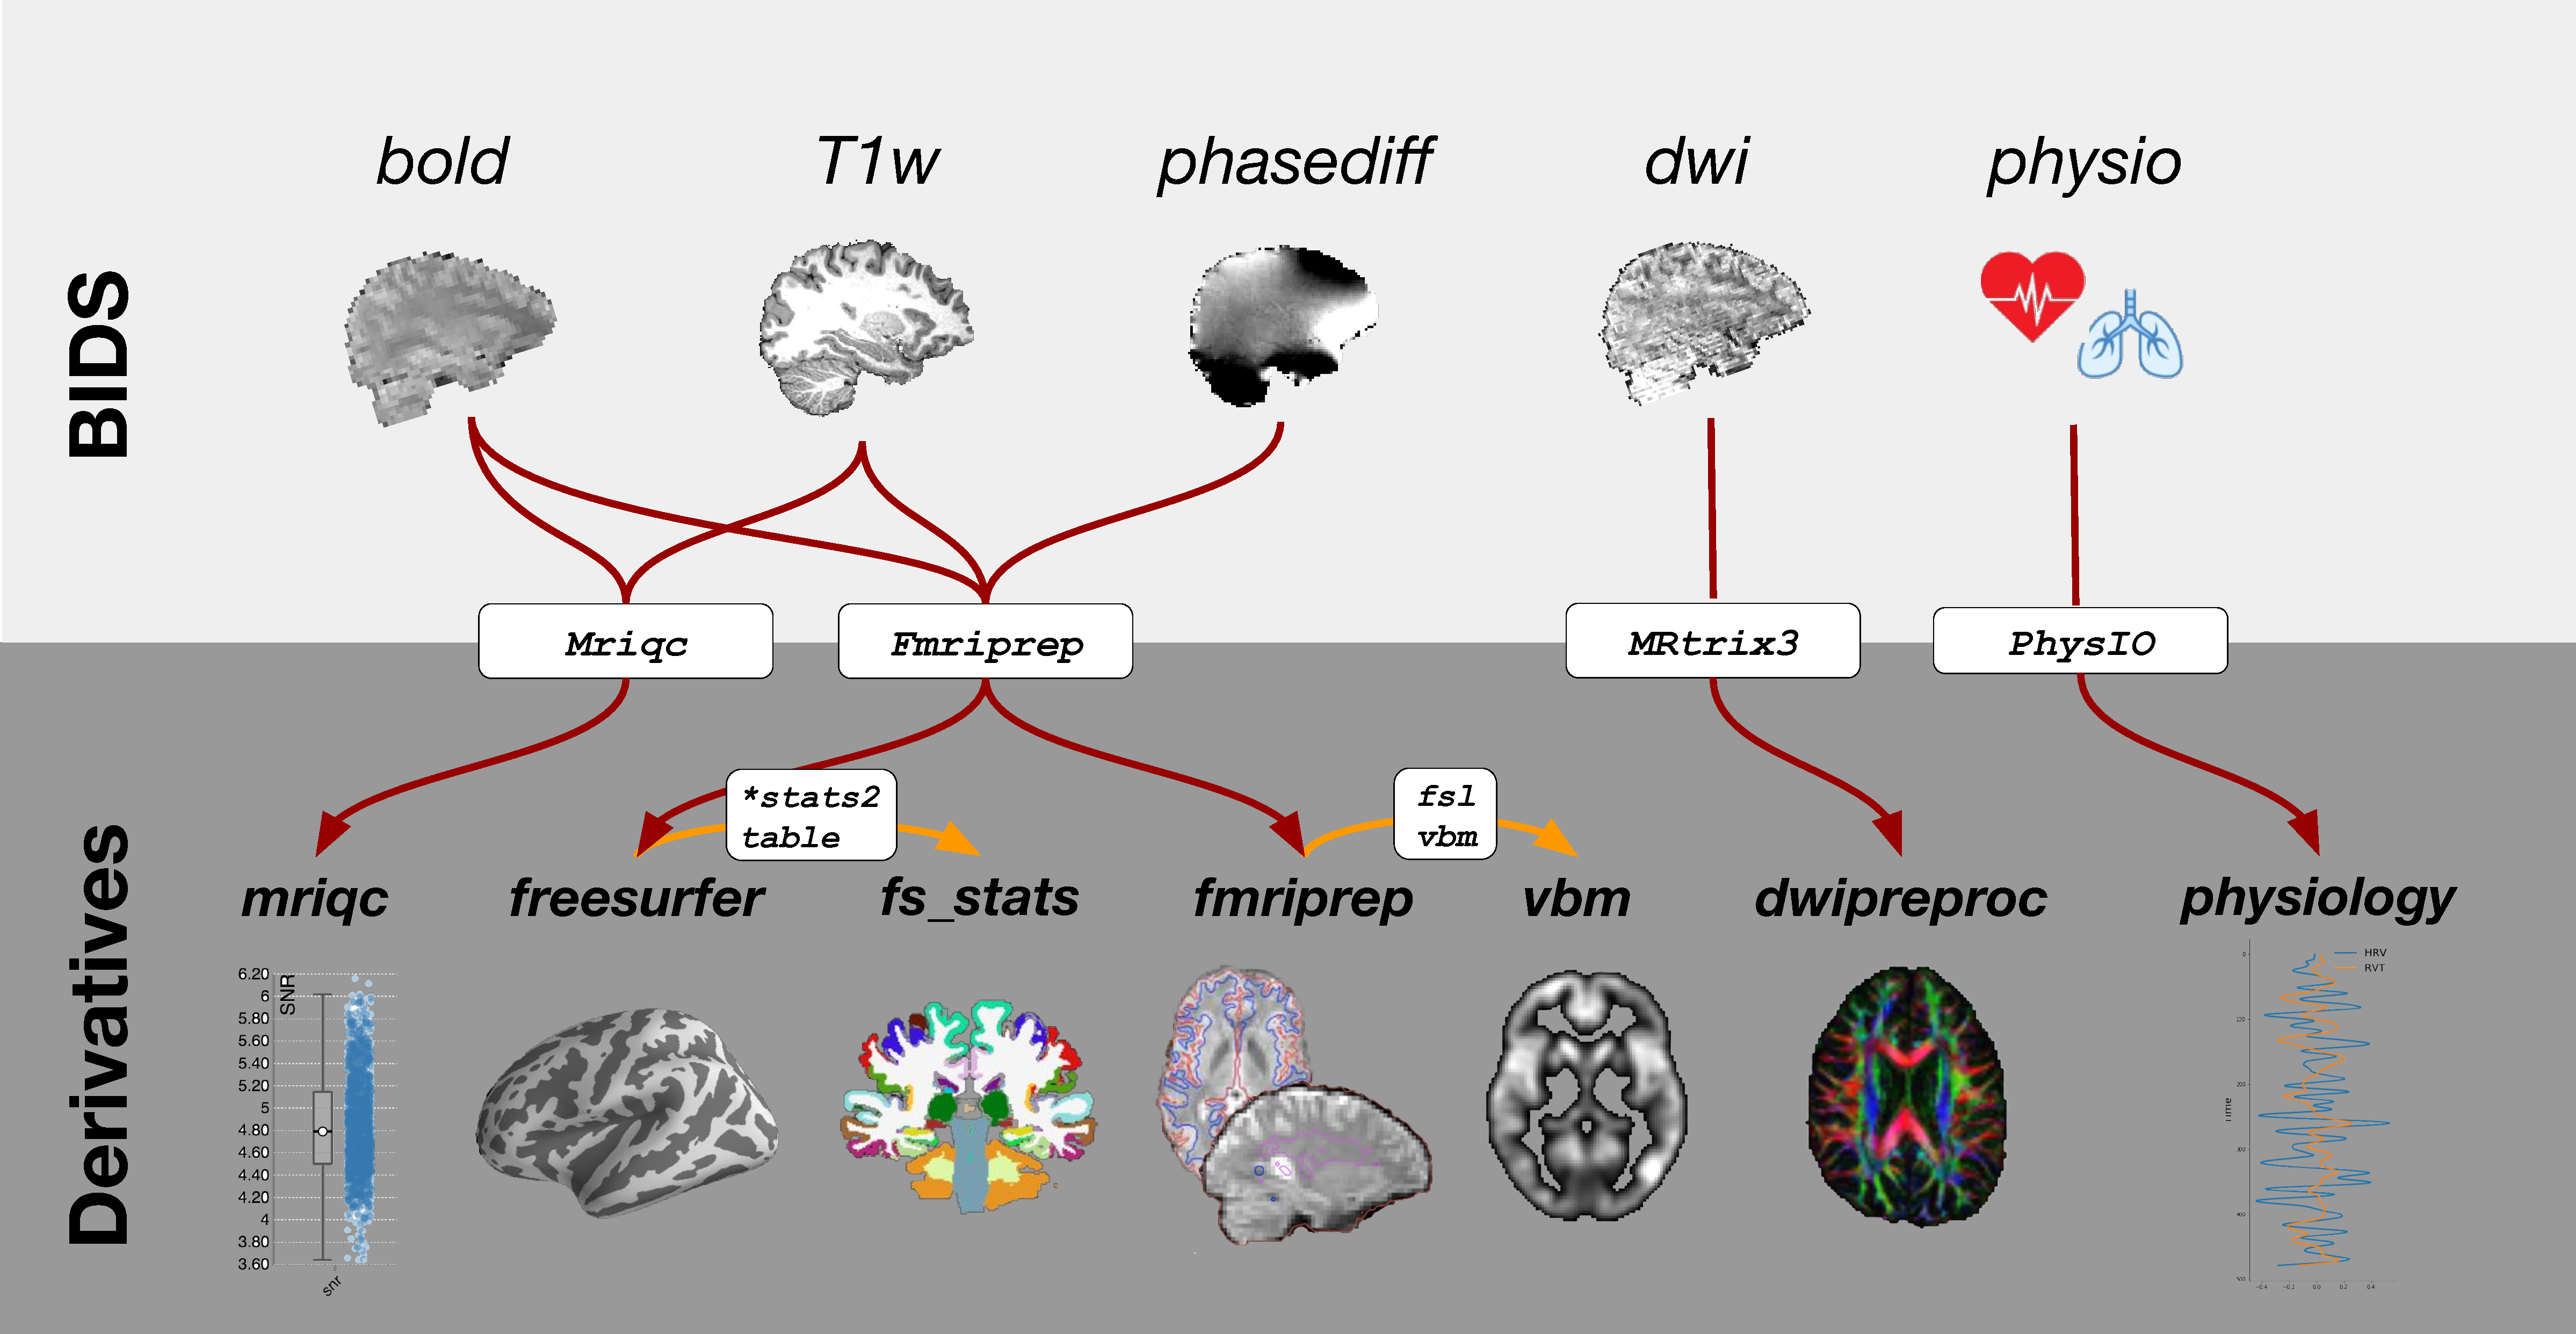
\includegraphics{_bookdown_files/aomic-files/figures/figure_3.pdf}
\caption{\label{fig:fig-aomic-3}Overview of the types of data and ``derivatives'' included in AOMIC and the software packages used to preprocess and analyze them.}
\end{figure}



\hypertarget{raw-data-standardization}{%
\subsubsection{Raw data standardization}\label{raw-data-standardization}}

Before subjecting the data to any preprocessing pipeline, we converted the data to BIDS using the in-house developed package bidsify (see \protect\hyperlink{aomic-code-availability}{Code availability} section for more details about the software used in the standardization process). The ``BIDSification'' process includes renaming of files according to BIDS convention, conversion from Philips PAR/REC format to compressed nifti, removal of facial characteristics from anatomical scans (``defacing''), and extraction of relevant metadata into JSON files.

The results from the standardization process were checked using the \emph{bids-validator} software package, which revealed no validation errors. However, the validation process raised several warnings about possible issues with the datasets (as shown in the BIDS validation section in their OpenNeuro repositories), which we explain in turn.

First, all three datasets contain subjects with incomplete data (i.e., missing MRI or physiology data), which causes the ``Not all subjects contain the same files'' warning. Second, the \emph{bids-validator} issues a warning that ``{[}n{]}ot all subjects/sessions/runs have the same scanning parameters''. One cause for this warning (in PIOP1 and PIOP2) is that the time to repetition (TR) parameter of some DWI scans varies slightly (PIOP1: \emph{min} = 7382 ms, \emph{max} = 7700, \emph{median} = 7390; PIOP2: \emph{min} = 7382, \emph{max} = 7519, \emph{median} = 7387), which is caused by acquiring the DWI data with the shortest possible TR (i.e., TR = ``shortest'' setting on Philips scanners; see Supplementary Tables \ref{tab:tab-aomic-S1}-\ref{tab:tab-aomic-S4}). Because the shortest possible TR depends on the exact angle of the slice box, the actual TR varies slightly from scan to scan. Notably, this warning is absent for the ID1000 dataset, because the TR value in the nifti file header is incorrect (i.e., it is set to 1 for each scan). Like the DWI scans in PIOP1 and PIOP2, the DWI scans from ID1000 were acquired with the shortest possible TR, resulting in slightly different TRs from scan to scan (\emph{min} = 6307, \emph{max} = 6838, \emph{median} = 6312). The correct TR values in seconds for each DWI scan in ID1000 was added to the dataset's \emph{participants.tsv} file (with the column names ``DWI\_TR\_run1'', ``DWI\_TR\_run2'', and ``DWI\_TR\_run3'').

In addition, the functional MRI scans from ID1000 were cropped in the axial and coronal direction by conservatively removing axial slices with low signal intensity in order to save disk space, causing slightly different dimensions across participants. Finally, in PIOP2, the functional MRI scans from the stop-signal task differ in the exact number of volumes (\emph{min} = 210, \emph{max} = 250, \emph{median} = 224) because the scan was stopped manually after the participant completed the task (which depended on their response times).

\hypertarget{anatomical-and-functional-mri-preprocessing}{%
\subsubsection{Anatomical and functional MRI preprocessing}\label{anatomical-and-functional-mri-preprocessing}}

Results included in this manuscript come from preprocessing performed using \emph{Fmriprep} version 1.4.1 (RRID:SCR\_016216; O. Esteban, Markiewicz, Blair, Moodie, Isik, Erramuzpe, Kent, Goncalves, DuPre, Snyder, Oya, et al., \protect\hyperlink{ref-Esteban2019-ri}{2019}; Esteban et al., \protect\hyperlink{ref-Esteban2020-qw}{2020}), a Nipype based tool (RRID:SCR\_002502; Gorgolewski et al., \protect\hyperlink{ref-Gorgolewski2011-aa}{2011}; Gorgolewski, Esteban, et al., \protect\hyperlink{ref-Gorgolewski2017-gb}{2017}). Each T1w (T1-weighted) volume was corrected for INU (intensity non-uniformity) using \emph{N4BiasFieldCorrection} v2.1.0 (Tustison et al., \protect\hyperlink{ref-Tustison2010-tk}{2010}) and skull-stripped using \emph{antsBrainExtraction.sh} v2.1.0 (using the OASIS template). Brain surfaces were reconstructed using recon-all from \emph{FreeSurfer} v6.0.1 (RRID:SCR\_001847; Dale et al., \protect\hyperlink{ref-Dale1999-rk}{1999}), and the brain mask estimated previously was refined with a custom variation of the method to reconcile ANTs-derived and FreeSurfer-derived segmentations of the cortical gray-matter of Mindboggle (RRID:SCR\_002438; Klein et al., \protect\hyperlink{ref-Klein2017-su}{2017}). Spatial normalization to the ICBM 152 Nonlinear Asymmetrical template version 2009c (RRID:SCR\_008796; Fonov et al., \protect\hyperlink{ref-Fonov2009-sr}{2009}) was performed through nonlinear registration with the \emph{antsRegistration} tool of ANTs v2.1.0 (RRID:SCR\_004757; Avants et al., \protect\hyperlink{ref-Avants2008-bv}{2008}), using brain-extracted versions of both T1w volume and template. Brain tissue segmentation of cerebrospinal fluid (CSF), white-matter (WM) and gray-matter (GM) was performed on the brain-extracted T1w using FSL \emph{fast} (FSL v5.0.9, RRID:SCR\_002823; Zhang et al., \protect\hyperlink{ref-Zhang2001-wa}{2001}).

Functional data was not slice-time corrected. Functional data was motion corrected using \emph{mcflirt} (FSL v5.0.9; Jenkinson et al., \protect\hyperlink{ref-Jenkinson2002-wm}{2002}) using the average volume after a first-pass motion correction procedure as the reference volume and normalized correlation as the image similarity cost function. ``Fieldmap-less'' distortion correction was performed by co-registering the functional image to the same-subject T1w image with intensity inverted (Huntenburg, \protect\hyperlink{ref-Huntenburg2014-ps}{2014}; Wang et al., \protect\hyperlink{ref-Wang2017-nk}{2017}), constrained with an average fieldmap template (Treiber et al., \protect\hyperlink{ref-Treiber2016-mc}{2016}), implemented with \emph{antsRegistration} (ANTs). Note that this fieldmap-less method was used even for PIOP2, which contained a phase-difference (B0) fieldmap, because we observed that Fmriprep's fieldmap-based method led to notably less accurate unwarping than its fieldmap-less method.

Distortion-correction was followed by co-registration to the corresponding T1w using boundary-based registration (Greve \& Fischl, \protect\hyperlink{ref-Greve2009-da}{2009}) with 6 degrees of freedom, using \emph{bbregister} (FreeSurfer v6.0.1). Motion correcting transformations, field distortion correcting warp, BOLD-to-T1w transformation and T1w-to-template (MNI) warp were concatenated and applied in a single step using \emph{antsApplyTransforms} (ANTs v2.1.0) using Lanczos interpolation.

Physiological noise regressors were extracted by applying \emph{CompCor} (Behzadi et al., \protect\hyperlink{ref-Behzadi2007-eb}{2007}). Principal components were estimated for the two \emph{CompCor} variants: temporal (\emph{tCompCor}) and anatomical (\emph{aCompCor}). A mask to exclude signal with cortical origin was obtained by eroding the brain mask, ensuring it only contained subcortical structures. Six \emph{tCompCor} components were then calculated including only the top 5\% variable voxels within that subcortical mask. For \emph{aCompCor}, six components were calculated within the intersection of the subcortical mask and the union of CSF and WM masks calculated in T1w space, after their projection to the native space of each functional run. Framewise displacement (Power et al., \protect\hyperlink{ref-Power2014-gh}{2014}) was calculated for each functional run using the implementation of \emph{Nipype}.

Many internal operations of Fmriprep use \emph{Nilearn} (RRID:SCR\_001362; Abraham et al., \protect\hyperlink{ref-Abraham2014-ef}{2014}), principally within the BOLD-processing workflow. For more details of the pipeline see
\url{https://fmriprep.readthedocs.io/en/1.4.1/workflows.html}.

\hypertarget{diffusion-mri-preprocessing}{%
\subsubsection{Diffusion MRI (pre)processing}\label{diffusion-mri-preprocessing}}

DWI scans were preprocessed using a custom pipeline combining tools from MRtrix3 (Tournier et al., \protect\hyperlink{ref-Tournier2019-hh}{2019}) and FSL. Because we acquired multiple DWI scans per participant in the ID1000 study (but not in PIOP1 and PIOP2), we concatenated these files as well as the diffusion gradient table (\emph{bvecs}) and b-value information (\emph{bvals}) prior to preprocessing. Using MRtrix3, we denoised the diffusion-weighted data using \emph{dwidenoise} (Veraart, Fieremans, et al., \protect\hyperlink{ref-Veraart2016-zi}{2016}; Veraart, Novikov, et al., \protect\hyperlink{ref-Veraart2016-rv}{2016}), removed Gibbs ringing artifacts using \emph{mrdegibbs} (Kellner et al., \protect\hyperlink{ref-Kellner2016-xb}{2016}), and performed eddy current and motion correction using \emph{dwipreproc}. Notably, \emph{dwipreproc} is a wrapper around the GPU-accelerated (CUDA v9.1) FSL tool \emph{eddy} (Andersson \& Sotiropoulos, \protect\hyperlink{ref-Andersson2016-pg}{2016}). Within \emph{eddy}, we used a quadratic first-level (\emph{--flm=quadratic}) and linear second-level model (\emph{--slm=linear}) and outlier replacement (Andersson et al., \protect\hyperlink{ref-Andersson2016-nm}{2016}) with default parameters (\emph{--repol}). Then, we performed bias correction using \emph{dwibiascorrect} (which is based on ANTs; v2.3.1), extracted a brain mask using \emph{dwi2mask} (Dhollander et al., \protect\hyperlink{ref-Dhollander2016-dx}{2016}), and corrected possible issues with the diffusion gradient table using \emph{dwigradcheck} (Jeurissen et al., \protect\hyperlink{ref-Jeurissen2014-cd}{2014}).

After preprocessing, using MRtrix3 tools, we fit a diffusion tensor model on the preprocessed diffusion-weighted data using weighted linear least squares (with 2 iterations) as implemented in \emph{dwi2tensor} (Veraart et al., \protect\hyperlink{ref-Veraart2013-ya}{2013}). From the estimated tensor image, a fractional anisotropy (FA) image was computed and a map with the first eigenvectors was extracted using \emph{tensor2metric}. Finally, a population FA template was computed using \emph{population\_template} (using an affine and an additional non-linear registration).

The following files are included in the DWI derivatives: a binary brain mask, the preprocessed DWI data as well as preprocessed gradient table (\emph{bvec}) and b-value (\emph{bval}) files, outputs from the eddy correction procedure (for quality control purposes; see \protect\hyperlink{aomic-technical-validation}{Technical validation} section), the estimated parameters from the diffusion tensor model, the eigenvectors from the diffusion tensor model, and a fractional anisotropy scalar map computed from the eigenvectors. All files are named according to BIDS Extension Proposal 16 (BEP016: diffusion weighted imaging derivatives).

\hypertarget{freesurfer-morphological-statistics}{%
\subsubsection{Freesurfer morphological statistics}\label{freesurfer-morphological-statistics}}

In addition to the complete Freesurfer directories containing the full surface reconstruction per participant, we provide a set of tab-separated values (TSV) files per participant with several morphological statistics per brain region for four different anatomical parcellations/segmentations. For cortical brain regions, we used two atlases shipped with Freesurfer: the Desikan-Killiany (\emph{aparc} in Freesurfer terms; Desikan et al., \protect\hyperlink{ref-Desikan2006-gh}{2006}) and Destrieux (\emph{aparc.a2009} in Freesurfer terms; Destrieux et al., \protect\hyperlink{ref-Destrieux2010-rd}{2010}) atlases. For these parcellations, the included morphological statistics are volume in mm\(^3\), area in mm\(^2\), thickness in mm, and integrated rectified mean curvature in mm\(^{-1}\). For subcortical and white matter brain regions, we used the results from the subcortical segmentation (\emph{aseg} in Freesurfer terms) and white matter segmentation (\emph{wmparc} in Freesurfer terms) done by Freesurfer. For these parcellations, the included morphological statistics are volume in mm\(^3\) and average signal intensity (arbitrary units). The statistics were extracted from the Freesurfer output directories using the Freesufer functions \emph{asegstats2table} and \emph{aparcstats2table} and further formatted using custom Python code. The TSV files (and accompanying JSON metadata files) are formatted according to BIDS Extension Proposal 11 (BEP011: structural preprocessing derivatives).

\hypertarget{voxel-based-morphology}{%
\subsubsection{Voxel-based morphology}\label{voxel-based-morphology}}

In addition to the Fmriprep-preprocessed anatomical T1-weighted scans, we also provide voxelwise gray matter volume maps estimated using voxel-based morphometry (VBM). We used a modified version of the FSL VBM pipeline (\url{http://fsl.fmrib.ox.ac.uk/fsl/fslwiki/FSLVBM}; Douaud et al., \protect\hyperlink{ref-Douaud2007-sw}{2007}), an optimised VBM protocol (Good, Johnsrude, et al., \protect\hyperlink{ref-Good2001-kv}{2001}\protect\hyperlink{ref-Good2001-kv}{b}) carried out with FSL tools (Smith et al., \protect\hyperlink{ref-Smith2004-sc}{2004}). We skipped the initial brain-extraction stage (\emph{fslvbm\_1\_bet}) and segmentation stage (first part of \emph{fslvbm\_3\_proc}) and instead used the probabilistic gray matter segmentation file (in native space) from \emph{Fmriprep} (i.e., \emph{label-GM\_probseg.nii.gz} files) directly. These files were registered to the MNI152 standard space using non-linear registration (Andersson et al., \protect\hyperlink{ref-Andersson2007-st}{2007}). The resulting images were averaged and flipped along the x-axis to create a left-right symmetric, study-specific grey matter template. Second, all native grey matter images were non-linearly registered to this study-specific template and ``modulated'' to correct for local expansion (or contraction) due to the non-linear component of the spatial transformation.

\hypertarget{physiological-noise-processing}{%
\subsubsection{Physiological noise processing}\label{physiological-noise-processing}}

Physiology files were converted to BIDS-compatible compressed TSV files using the \emph{scanphyslog2bids} package (see \protect\hyperlink{aomic-code-availability}{Code availability}). Each TSV file contains three columns: the first contains the cardiac trace, the second contains the respiratory trace, and the third contains the volume onset triggers (binary, where 1 represents a volume onset). Each TSV file is accompanied by a JSON metadata file with the same name, which contains information about the start time of the physiology recording relative to the onset of the first volume. Because the physiology recording always starts before the fMRI scan starts, the start time is always negative (e.g., a start time of -42.01 means that the physiology recording started 42.01 seconds before the onset of the first volume). After conversion to BIDS, the estimated volume triggers and physiology traces were plotted, visually inspected for quality, and excluded if either of the physiology traces had missing data for more than ten seconds or if the volume triggers could not be estimated.

The physiology data was subsequently used to estimate fMRI-appropriate nuisance regressors using the \emph{TAPAS PhysIO} package (Kasper et al., \protect\hyperlink{ref-Kasper2017-lp}{2017}). Using this package, we specifically estimated 18 ``RETROICOR'' regressors (Glover et al., \protect\hyperlink{ref-Glover2000-or}{2000}) based on a Fourier expansion of cardiac (order: 2) and respiratory (order: 3) phase and their first-order multiplicative terms (as defined in Harvey et al., \protect\hyperlink{ref-Harvey2008-nt}{2008}). In addition, we estimated a heart-rate variability (HRV) regressor by convolving the cardiac trace with a cardiac response function (Chang et al., \protect\hyperlink{ref-Chang2009-vu}{2009}) and a respiratory volume by time (RVT) regressor by convolving the respiratory trace with a respiration response function (Birn et al., \protect\hyperlink{ref-Birn2008-ti}{2008}).

\hypertarget{data-records}{%
\section{Data records}\label{data-records}}

\hypertarget{data-formats-and-types}{%
\subsection{Data formats and types}\label{data-formats-and-types}}

In AOMIC, the majority of the data is stored in one of four formats. First, all volumetric (i.e., 3D or 4D) MRI data is stored in compressed ``NIfTI'' files (NIfTI-1 version; extension: \emph{.nii.gz}). NIfTI files contain both the data and metadata (stored in the header) and can be loaded into all major neuroimaging analysis packages and programming languages using, e.g., the \emph{nibabel} package for Python (\url{https://nipy.org/nibabel}), the \emph{oro.nifti} package in R (\url{https://cran.r-project.org/web/packages/oro.nifti}), and natively in Matlab (version R2017b and higher). Second, surface (i.e., vertex-wise) MRI data is stored in ``Gifti'' files (\url{https://www.nitrc.org/projects/gifti}; extension: \emph{.gii}). Like NIfTI files, Gifti files contain both data and metadata and can be loaded in several major neuroimaging software packages (including Freesurfer, FSL, AFNI, SPM, and Brain Voyager) and programming languages using, e.g., the \emph{nibabel} package for Python and the \emph{gifti} package for R (\url{https://cran.rstudio.com/web/packages/gifti}).

Third, data organized as tables (i.e., observations in rows and properties in columns), such as physiological data and task-fMRI event log files, are stored in tab-separated values (TSV) files, which contain column names as the first row. TSV files can be opened using spreadsheet software (such as Microsoft Excel or Libreoffice Calc) and read using most major programming languages. Fourth, (additional) metadata is stored as key-value pairs in plain-text JSON files. A small minority of data in AOMIC is stored using different file formats (such as \emph{hdf5} for composite transforms of MRI data and some Freesurfer files), but these are unlikely to be relevant for most users.

Apart from data \emph{formats}, we can distinguish different data \emph{types} within AOMIC. Following BIDS convention, data types are distinguished based on an ``identifier'' at the end of the file name (before the extension). For example, T1-weighted files (e.g., \emph{sub-0001\_T1w.nii.gz}) are distinguished by the *\_T1w* identifier and event log files for task-based functional MRI data (e.g., \emph{sub-001\_task-workingmemory\_acq-seq\_events.tsv}) are distinguished by the *\_events* identifier. All data types and associated identifiers within AOMIC are listed in Supplementary Table \ref{tab:tab-aomic-S6}.

\hypertarget{data-repositories-used}{%
\subsection{Data repositories used}\label{data-repositories-used}}

Data from AOMIC can be subdivided into two broad categories. The first category encompasses all subject-level data, both raw data and derivatives. The second category encompasses group-level aggregates of data, such as an average (across subjects) tSNR map or group-level task fMRI activation maps. Data from these two categories are stored in separate, dedicated repositories: subject-level data is stored on OpenNeuro (\url{https://openneuro.org}; K Gorgolewski et al., \protect\hyperlink{ref-Gorgolewski2017-uu}{2017})
and the subject-aggregated data is stored on NeuroVault (\url{https://neurovault.org}; Gorgolewski, Varoquaux, Rivera, Schwarz, Ghosh, Maumet, Sochat, Nichols, Poldrack, Poline, Yarkoni, et al., \protect\hyperlink{ref-Gorgolewski2015-hj}{2015}). Data from each dataset --- PIOP1, PIOP2, and ID1000 --- are stored in separate repositories on OpenNeuro (L. Snoek et al., \protect\hyperlink{ref-Snoek2020-id1000}{2020}\protect\hyperlink{ref-Snoek2020-id1000}{b}, \protect\hyperlink{ref-Snoek2020-piop1}{2020}\protect\hyperlink{ref-Snoek2020-piop1}{d}, \protect\hyperlink{ref-Snoek2020-piop2}{2020}\protect\hyperlink{ref-Snoek2020-piop2}{f}) and NeuroVault (L. Snoek et al., \protect\hyperlink{ref-Snoek2020n-id1000}{2020}\protect\hyperlink{ref-Snoek2020n-id1000}{a}, \protect\hyperlink{ref-Snoek2020n-piop1}{2020}\protect\hyperlink{ref-Snoek2020n-piop1}{c}, \protect\hyperlink{ref-Snoek2020n-piop2}{2020}\protect\hyperlink{ref-Snoek2020n-piop2}{e}). URLs to these repositories for all datasets can be found in Table \ref{tab:tab-aomic-5}. Apart from the option to download data using a web browser, we provide instructions to download the data programmatically on \url{https://nilab-uva.github.io/AOMIC.github.io}.

\begingroup\fontsize{10}{12}\selectfont

\begin{ThreePartTable}
\begin{TableNotes}[para]
\item \textit{Note: } 
\item To go to the OpenNeuro web repositories, prefix the OpenNeuro ID with "https://openneuro.org/datasets/". To go to the NeuroVault web repositories, prefix the NeuroVault ID with "https://neurovault.org/collections/".
\end{TableNotes}
\begin{longtabu} to \linewidth {>{\raggedright}X>{\raggedright}X>{\raggedright}X>{\raggedright}X}
\caption{\label{tab:tab-aomic-5}Data repository identifiers for subject data (OpenNeuro) and group-level data (NeuroVault).}\\
\toprule
Repository & ID1000 & PIOP1 & PIOP2\\
\midrule
OpenNeuro ID & ds003097 & ds002785 & ds002790\\
Neurovault ID & 7105 & 7103 & 7104\\
\bottomrule
\insertTableNotes
\end{longtabu}
\end{ThreePartTable}
\endgroup{}

\hypertarget{data-anonymization}{%
\subsubsection{Data anonymization}\label{data-anonymization}}

In curating this collection, we took several steps in ensuring the anonymity of participants. All measures were discussed with the data protection officer of the University of Amsterdam and the data steward of the department of psychology, who deemed the anonymized data to be in accordance with the European General Data Protection Regulation (GDPR).

First, all personally identifiable information (such as subjects' name, date of birth, and contact information) in all datasets were irreversibly destroyed. Second, using the \emph{pydeface} software package (Gulban et al., \protect\hyperlink{ref-Gulban2019-sv}{2019}), we removed facial characteristics (mouth and nose) from all anatomical scans, i.e., the T1-weighted anatomical scans and (in PIOP2) magnitude and phase-difference images from the B0 fieldmap. The resulting defaced images were checked visually to confirm that the defacing succeeded. Third, the data files were checked for timestamps and removed when present. Lastly, we randomized the subject identifiers (\emph{sub-xxxx}) for all files. In case participants might have remembered their subject number, they will not be able to look up their own data within our collection.

\hypertarget{technical-validation}{%
\section{Technical validation}\label{technical-validation}}

In this section, we describe the measures taken for quality control of the data. This is described per data type (e.g., anatomical T1-weighted images, DWI images, physiology, etc.), rather than per dataset, as the procedure for quality control per data type was largely identical across the datasets. Importantly, we take a conservative approach towards exclusion of data, i.e., we generally did not exclude data unless (1) it was corrupted by scanner-related incorrigible artifacts, such as reconstruction errors, (2) when preprocessing fails due to insufficient data quality (e.g., in case of strong spatial inhomogeneity of structural T1-weighted scans, preventing accurate segmentation), (3) an absence of a usable T1-weighted scan (which is necessary for most preprocessing pipelines), or (4) incidental findings. This way, the data from AOMIC can also be used to evaluate artifact-correction methods and other preprocessing techniques aimed to post-hoc improve data quality and, importantly, this places the responsibility for inclusion and exclusion of data in the hands of the users of the datasets.

Researchers not interested in using AOMIC data for artifact-correction or preprocessing techniques may still want to exclude data that do not meet their quality standards. As such, we include, for each modality (T1-weighted, BOLD, and DWI) separately, a file with several quality control metrics across subjects. The quality control metrics for the T1-weighted and functional (BOLD) MRI scans were computed by the Mriqc package (O. Esteban, Birman, et al., \protect\hyperlink{ref-Esteban2017-mv}{2017}) and are stored in the \emph{group\_T1w.tsv} and \emph{group\_T1w.tsv} files in the \emph{mriqc} derivatives folder. The quality control metrics for the DWI scans were derived from the output of FSL's \emph{eddy} algorithm and are stored in the \emph{group\_dwi.tsv} file in the dwipreproc derivatives folder. Using these precomputed quality control metrics, researchers can decide which data to include based on their own quality criteria.

\hypertarget{t1-weighted-scans}{%
\subsection{T1-weighted scans}\label{t1-weighted-scans}}

All T1-weighted scans were run through the \emph{Mriqc} pipeline, which outputs several quality control metrics as well as a report with visualizations of different aspects of the data. All individual subject reports were visually checked for artifacts including reconstruction errors, failure of defacing, normalization issues, and segmentation issues (and the corresponding data excluded when appropriate). In Figure \ref{fig:fig-aomic-4}, we visualize several quality control metrics related to the T1-weighted scans across all three datasets. In general, data quality appears to increase over time (with ID1000 being the oldest dataset, followed by PIOP1 and PIOP2), presumably due to improvements in hardware (see Scanner details and general scanning protocol). All quality control metrics related to the T1-weighted scans, including those visualized in Figure \ref{fig:fig-aomic-4}, are stored in the \emph{group\_T1w.tsv} file in the \emph{mriqc} derivatives folder.

\begin{figure}
\centering
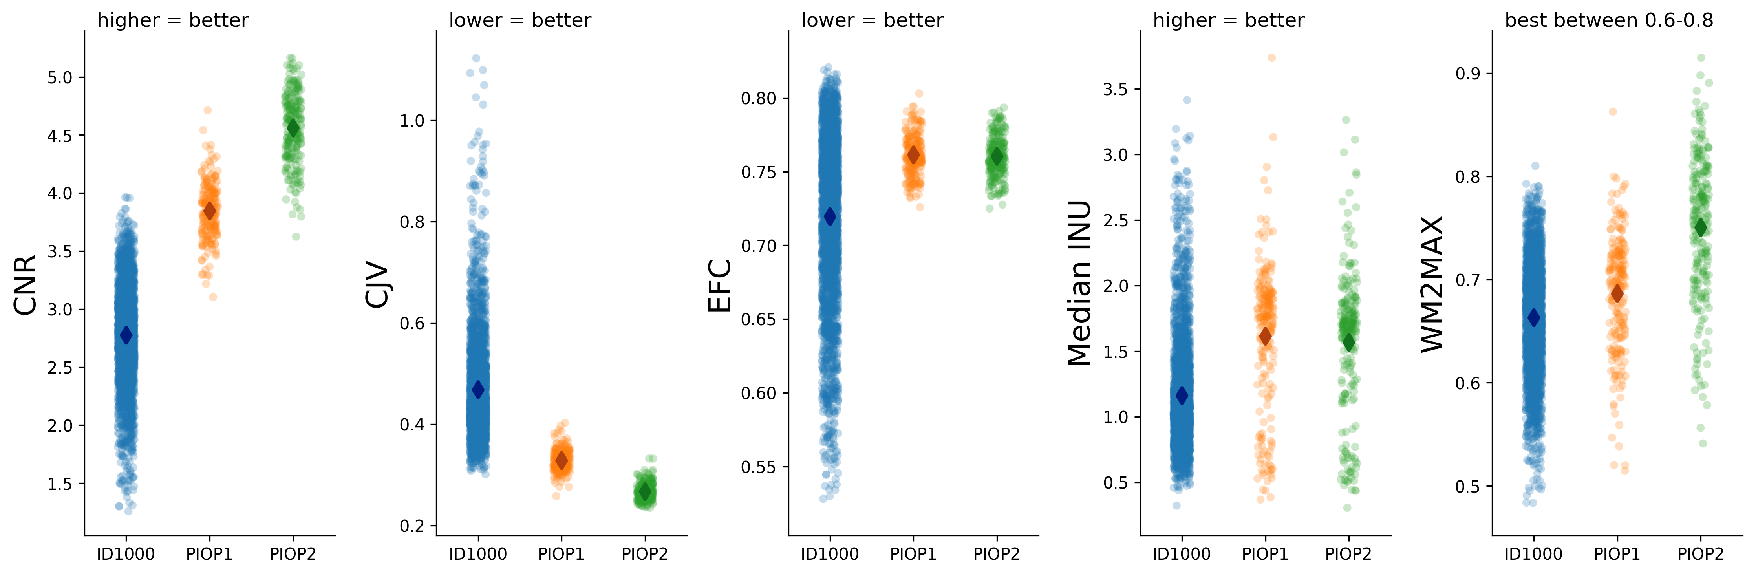
\includegraphics{_bookdown_files/aomic-files/figures/figure_4.pdf}
\caption{\label{fig:fig-aomic-4}Quality control metrics related to the T1-weighted scans. CNR: contrast-to-noise ratio (Magnotta et al., \protect\hyperlink{ref-Magnotta2006-zs}{2006}); CJV: coefficient of joint variation (Ganzetti et al., \protect\hyperlink{ref-Ganzetti2016-yy}{2016}), an index reflecting head motion and spatial inhomogeneity; EFC: entropy-focused criterion (Atkinson et al., \protect\hyperlink{ref-Atkinson1997-eu}{1997}), an index reflecting head motion and ghosting; INU: intensity non-uniformity, an index of spatial inhomogeneity; WM2MAX: ratio of median white-matter intensity to the 95\% percentile of all signal intensities; low values may lead to problems with tissue segmentation.}
\end{figure}



\hypertarget{functional-bold-scans}{%
\subsection{Functional (BOLD) scans}\label{functional-bold-scans}}

Like the T1-weighted images, the functional (BOLD) scans were run through the Mriqc pipeline. The resulting reports were visually checked for artifacts including reconstruction errors, registration issues, and incorrect brain masks.

In Figure \ref{fig:fig-aomic-5}, we visualize several quality control metrics related to the functional scans across all three datasets. Similar to the T1-weighted quality control metrics, the functional quality control metrics indicate an improvement of quality over time. Also note the clear decrease in temporal signal-to-noise ratio (tSNR) for multiband-accelerated scans (consistent with Demetriou et al. (\protect\hyperlink{ref-Demetriou2018-xp}{2018})). All quality control metrics related to the functional MRI scans, including those visualized in Figure \ref{fig:fig-aomic-5}, are stored in the \emph{group\_bold.tsv} file in the \emph{mriqc} derivatives folder.

\begin{figure}
\centering
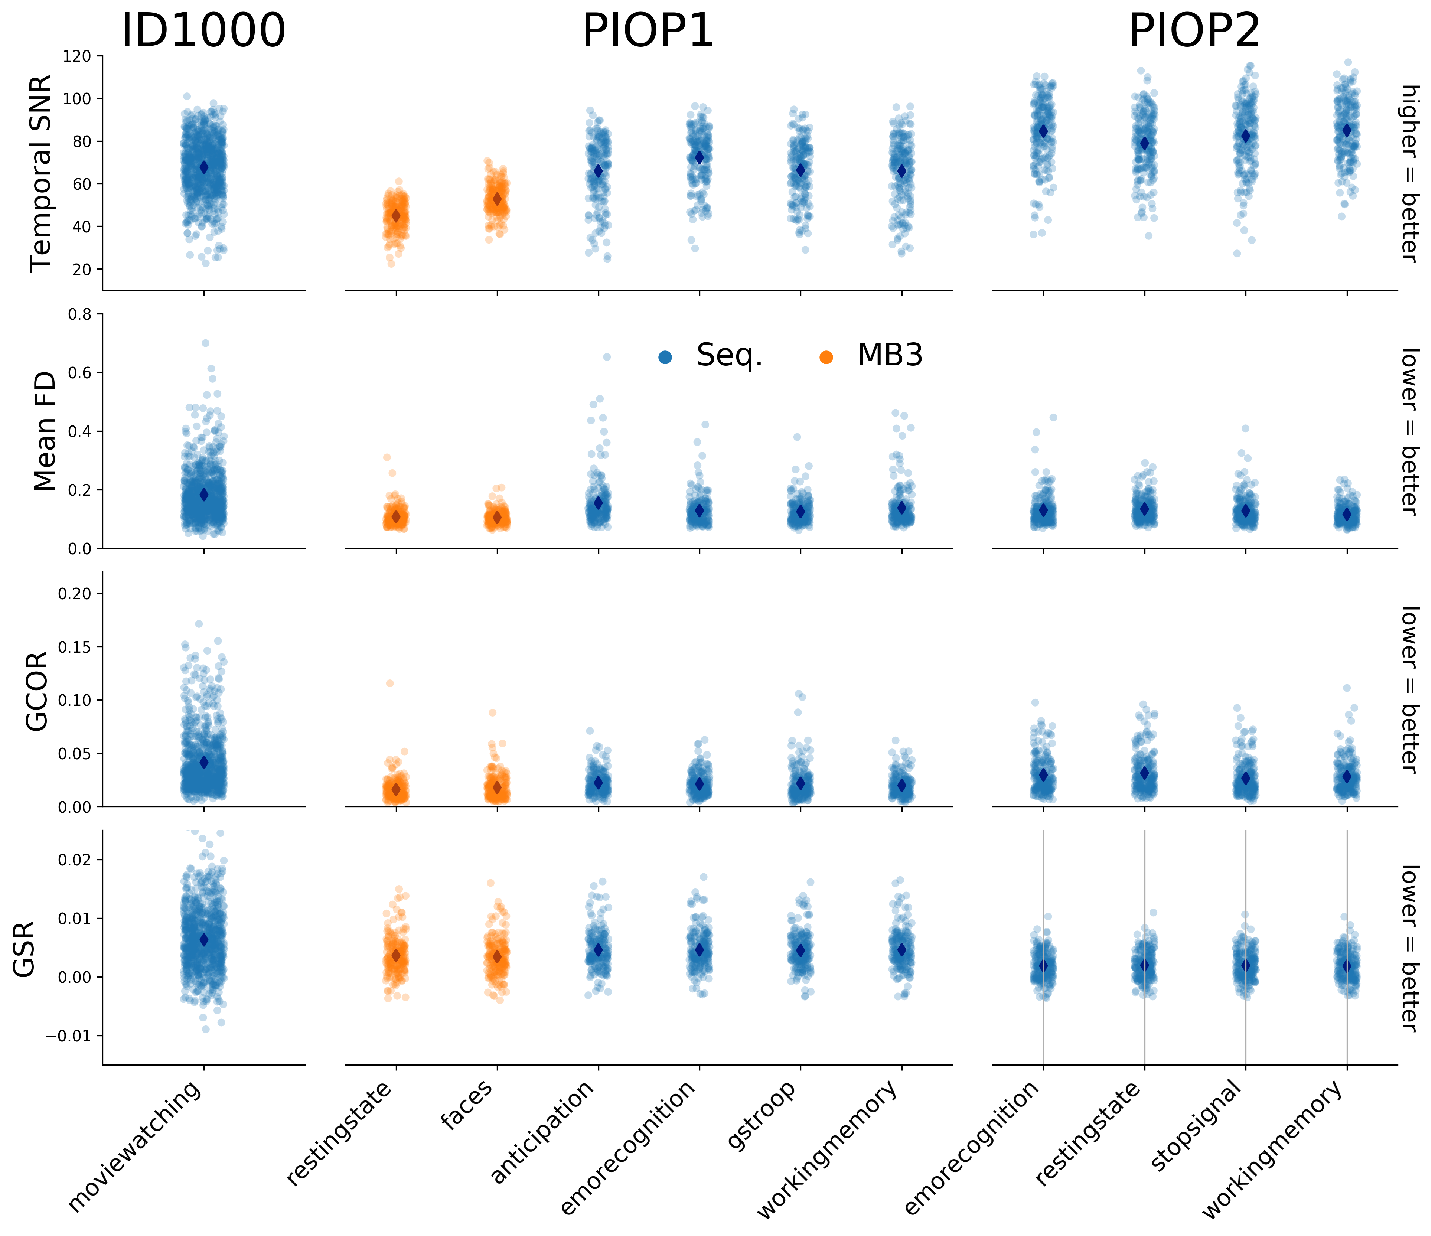
\includegraphics{_bookdown_files/aomic-files/figures/figure_5.pdf}
\caption{\label{fig:fig-aomic-5}Quality control metrics related to the functional (BOLD) MRI scans. SNR: signal-to-noise ratio, an index of signal quality; FD: framewise displacement (Power et al., \protect\hyperlink{ref-Power2012-kt}{2012}), an index of overall movement; GCOR: global correlation, an index of the presence of global signals (Saad et al., \protect\hyperlink{ref-Saad2013-zd}{2013}); GSR: ghost-to-signal ratio, an index of ghosting along the phase-encoding axis.}
\end{figure}



In Figure \ref{fig:fig-aomic-6}, we visualize these tSNR maps for each dataset (and separately for the sequential and multiband scans of PIOP1). Again, there appears to be an increase in tSNR across time. Corresponding whole-brain tSNR maps can be viewed and downloaded from NeuroVault (i.e., files with the *\_tsnr* identifier).

\begin{figure}
\centering
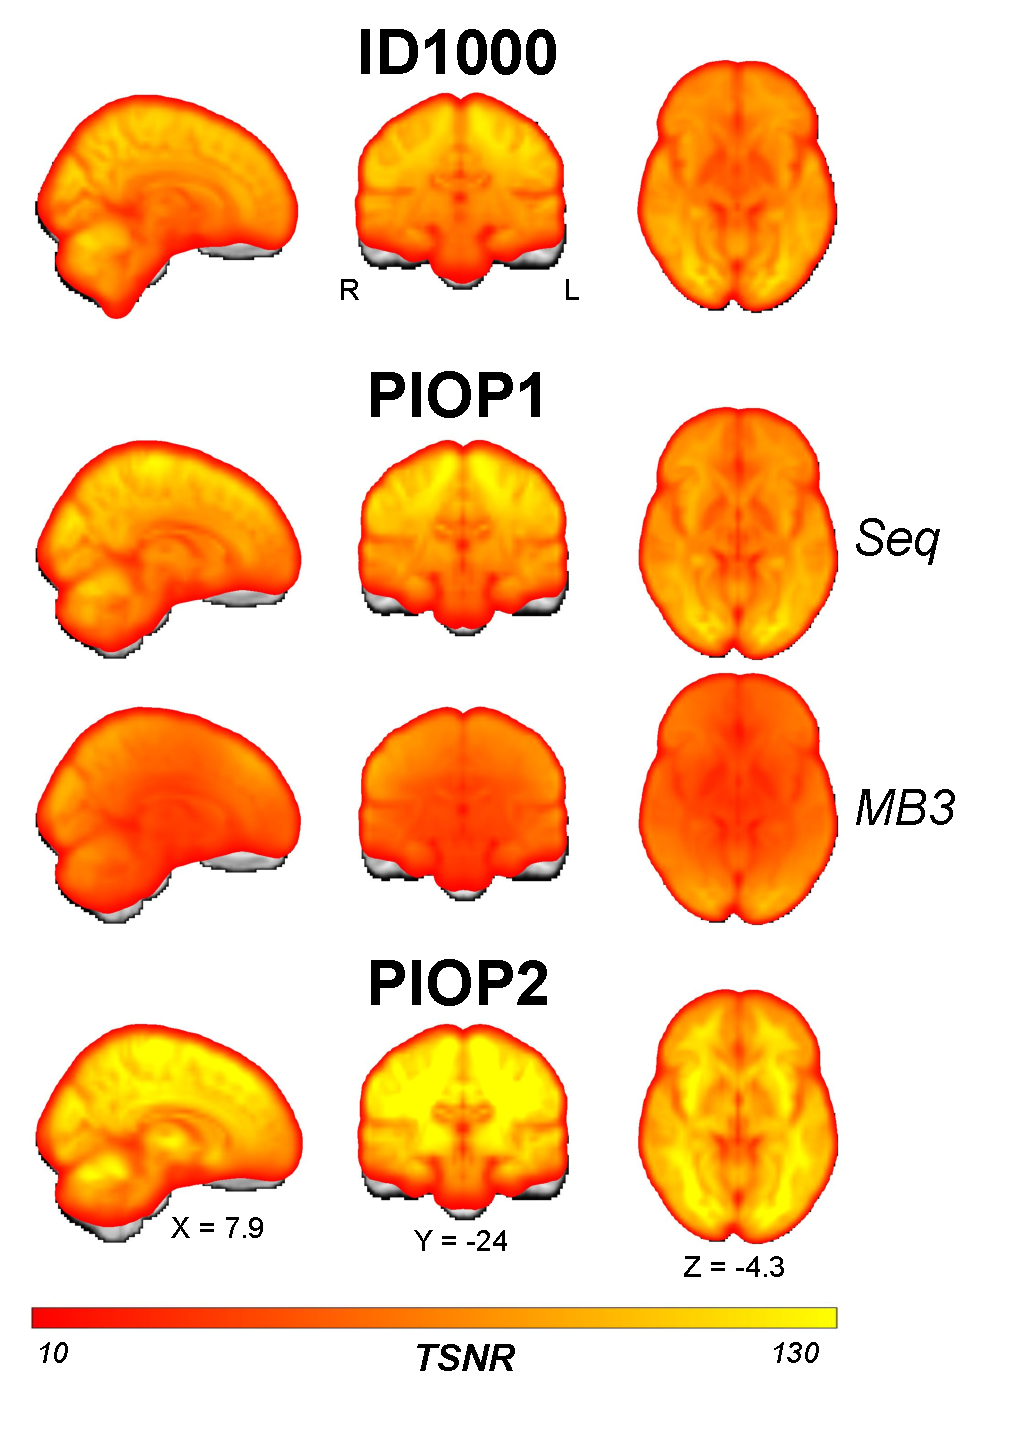
\includegraphics{_bookdown_files/aomic-files/figures/figure_6.pdf}
\caption{\label{fig:fig-aomic-6}Average (across subjects and runs) temporal signal-to-noise (tSNR) maps of each type of functional (BOLD) MRI scan in each dataset. Unthresholded whole-brain tSNR maps are available on NeuroVault.}
\end{figure}



For the fMRI data with an explicit task (i.e., all fMRI data except for the PIOP resting-state fMRI scans and the ID1000 movie watching fMRI scan), we additionally computed group-level whole-brain statistics maps. To do so, using the \emph{nistats} Python package, we ran mass-univariate first-level GLS models (using an AR1 noise model) based on a design matrix including task-regressors based on the events convolved with a canonical HRF function as well as a discrete cosine basis set functioning as a high-pass filter of 128 seconds and six motion regressors and computed first-level contrast maps for each subject which were subsequently analyzed in a random effects group-level (intercept) model, resulting in whole-brain \emph{z}-value maps. The data was never spatially smoothed. In Figure \ref{fig:fig-aomic-7}, we show the (uncorrected) whole-brain group-level results for each task. Note that we chose these specific contrasts to demonstrate that the tasks elicit to-be expected effects (e.g., amygdala activity in the emotion matching task and cingulate cortex activity in the gender-stroop task). Different, and more sophisticated analyses, including analysis of between-subject factors, are possible with this data and the associated event files.

\begin{figure}
\centering
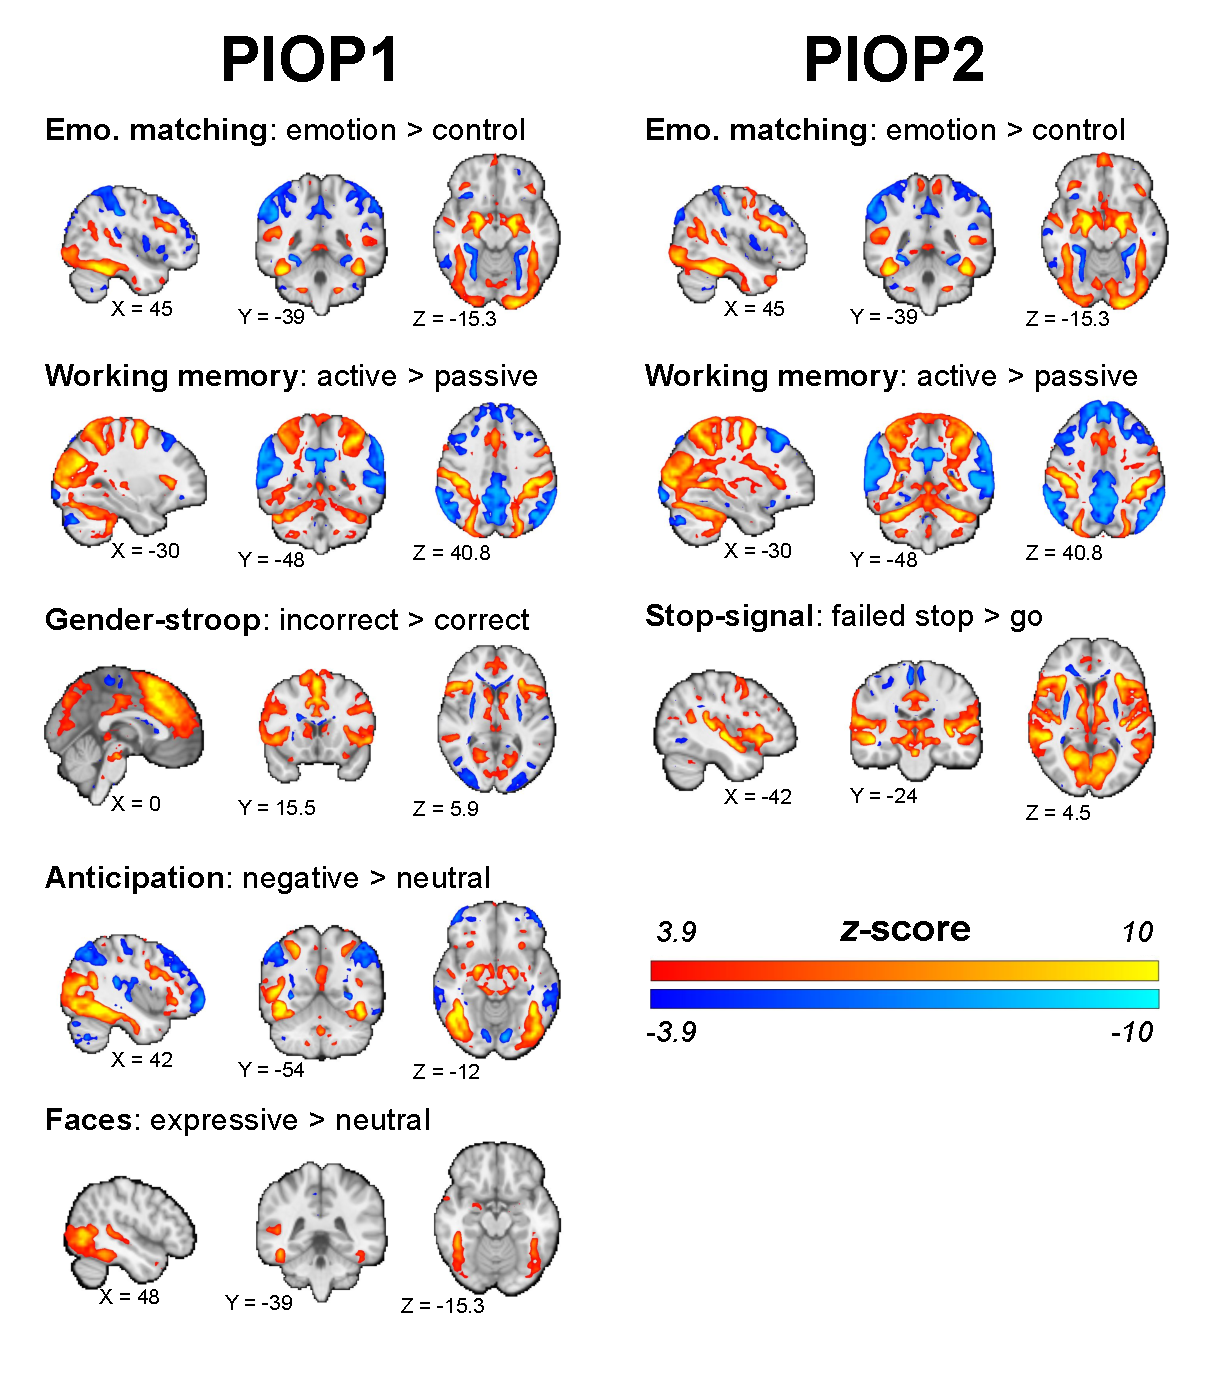
\includegraphics{_bookdown_files/aomic-files/figures/figure_7.pdf}
\caption{\label{fig:fig-aomic-7}Results from task-specific group-level analyses. Brain maps show uncorrected effects (\emph{p} \textless{} 0.00001, two-sided) and were linearly interpolated for visualization in \emph{FSLeyes}. Unthresholded whole-brain \emph{z}-value maps are available on NeuroVault. Unthresholded whole-brain \emph{z}-value maps are available on NeuroVault.}
\end{figure}



To validate the quality of the resting-state functional MRI scans in PIOP1 and PIOP2, we ran dual regression analyses (Beckmann et al., \protect\hyperlink{ref-Beckmann2009-rs}{2009}) using the spatial ICA maps from Smith and colleagues (10-component version; Smith et al., \protect\hyperlink{ref-Smith2009-kj}{2009}). Prior to the dual regression analyses, the data was cleaned and high-pass filtered (using a 128 second cutoff) by regressing out a discrete cosine basis set and six motion parameter estimates and spatially smoothed with a Gaussian kernel with a 5 mm FWHM. Figure \ref{fig:fig-aomic-8} shows the group-level dual regression results from both PIOP1 and PIOP2 for the first four components next to the original ICA map from Smith et al. (\protect\hyperlink{ref-Smith2009-kj}{2009}).

\begin{figure}
\centering
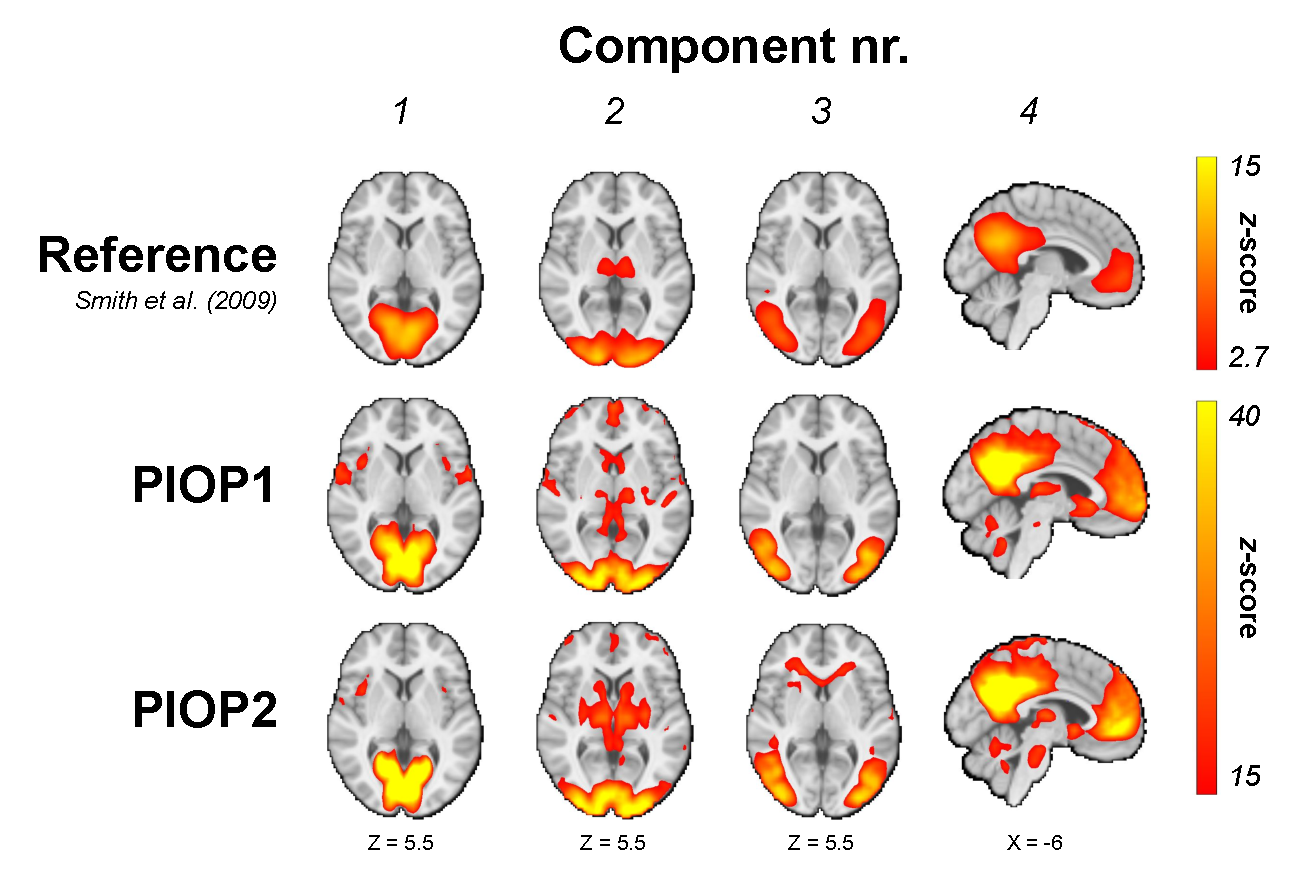
\includegraphics{_bookdown_files/aomic-files/figures/figure_8.pdf}
\caption{\label{fig:fig-aomic-8}Group-level dual regression results for the first four components of Smith and colleagues (2009). Unthresholded \emph{z}-value maps are available on NeuroVault.}
\end{figure}



Finally, to assess the quality of the ID1000 functional MRI data, we performed a voxelwise whole-brain ``inter-subject correlation'' (ISC) analysis (Hasson et al., \protect\hyperlink{ref-Hasson2004-xb}{2004}), using the BrainIAK software package (Kumar et al., \protect\hyperlink{ref-Kumar2020-eo}{2020}) on data from a subset of 100 participants (randomly drawn from the ID1000 dataset). Before computing the inter-subject correlations, the data were masked by an intersection of a functional brain mask and a grey matter mask (probability \textgreater{} 0.1). Low-frequency drift (with a cutoff of 128 seconds), the mean signal within the cerebrospinal fluid, global (whole-brain average) signal, and six motion parameters were regressed out before computing the ISCs. The average (across subjects) voxelwise ISCs are visualized in Figure \ref{fig:fig-aomic-9}, which shows the expected inter-subject synchrony in the ventral and dorsal visual stream. The emphasis on variance in visual parameters rather than narrative when composing the movie stimulus likely caused the high ISC values to be largely restricted to visual brain areas.

\begin{figure}
\centering
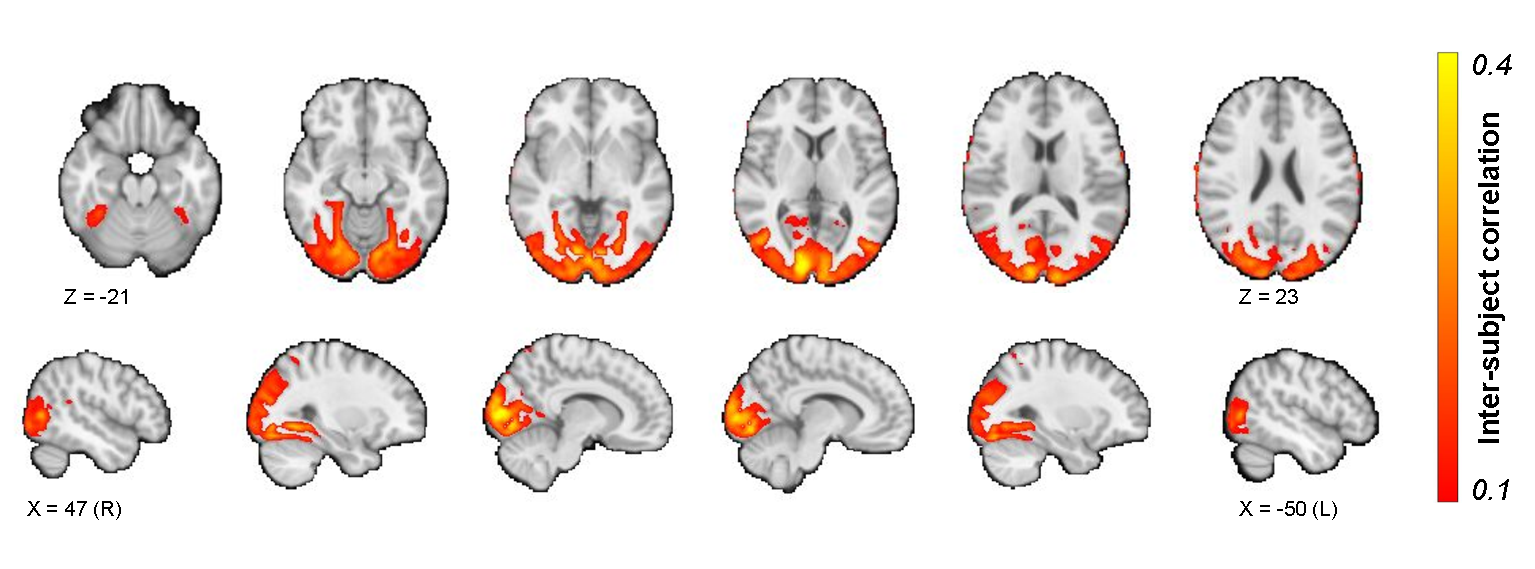
\includegraphics{_bookdown_files/aomic-files/figures/figure_9.pdf}
\caption{\label{fig:fig-aomic-9}Results from the voxelwise ISC analysis, arbitrarily thresholded at 0.1. An unthresholded whole-brain ISC map is available on NeuroVault.}
\end{figure}



\hypertarget{diffusion-weighted-scans}{%
\subsection{Diffusion-weighted scans}\label{diffusion-weighted-scans}}

Before preprocessing, the b=0 volume from each DWI scan was extracted and visually checked for severe artifacts and reconstruction errors (in which case the data was excluded). After preprocessing and DTI model fitting, we furthermore visualized each estimated fractional anisotropy (FA) map and the color-coded FA-modulated (absolute) eigenvectors for issues with the gradient directions. These images are included in the DWI derivatives.

Furthermore, we extracted quality control metrics based on outputs from the eddy correction/motion correction procedure in the DWI preprocessing pipeline as implemented in FSL's \emph{eddy} algorithm (based on the procedure outlined in Bastiani et al. (\protect\hyperlink{ref-Bastiani2019-sm}{2019})). Specifically, we computed the mean framewise displacement across volumes based on the realignment parameters from motion correction, the percentage of ``outlier slices'' (as determined by FSL \emph{eddy}) in total and per volume, and the standard deviation of the estimated linear eddy current distortions across volumes. These metrics are visualized in Figure \ref{fig:fig-aomic-10}. Note that the y-axis for the standard deviation of the eddy currents for ID1000 has a larger range than for PIOP1 and PIOP2 to show the scans with particularly strong eddy current fluctuations.

\begin{figure}
\centering
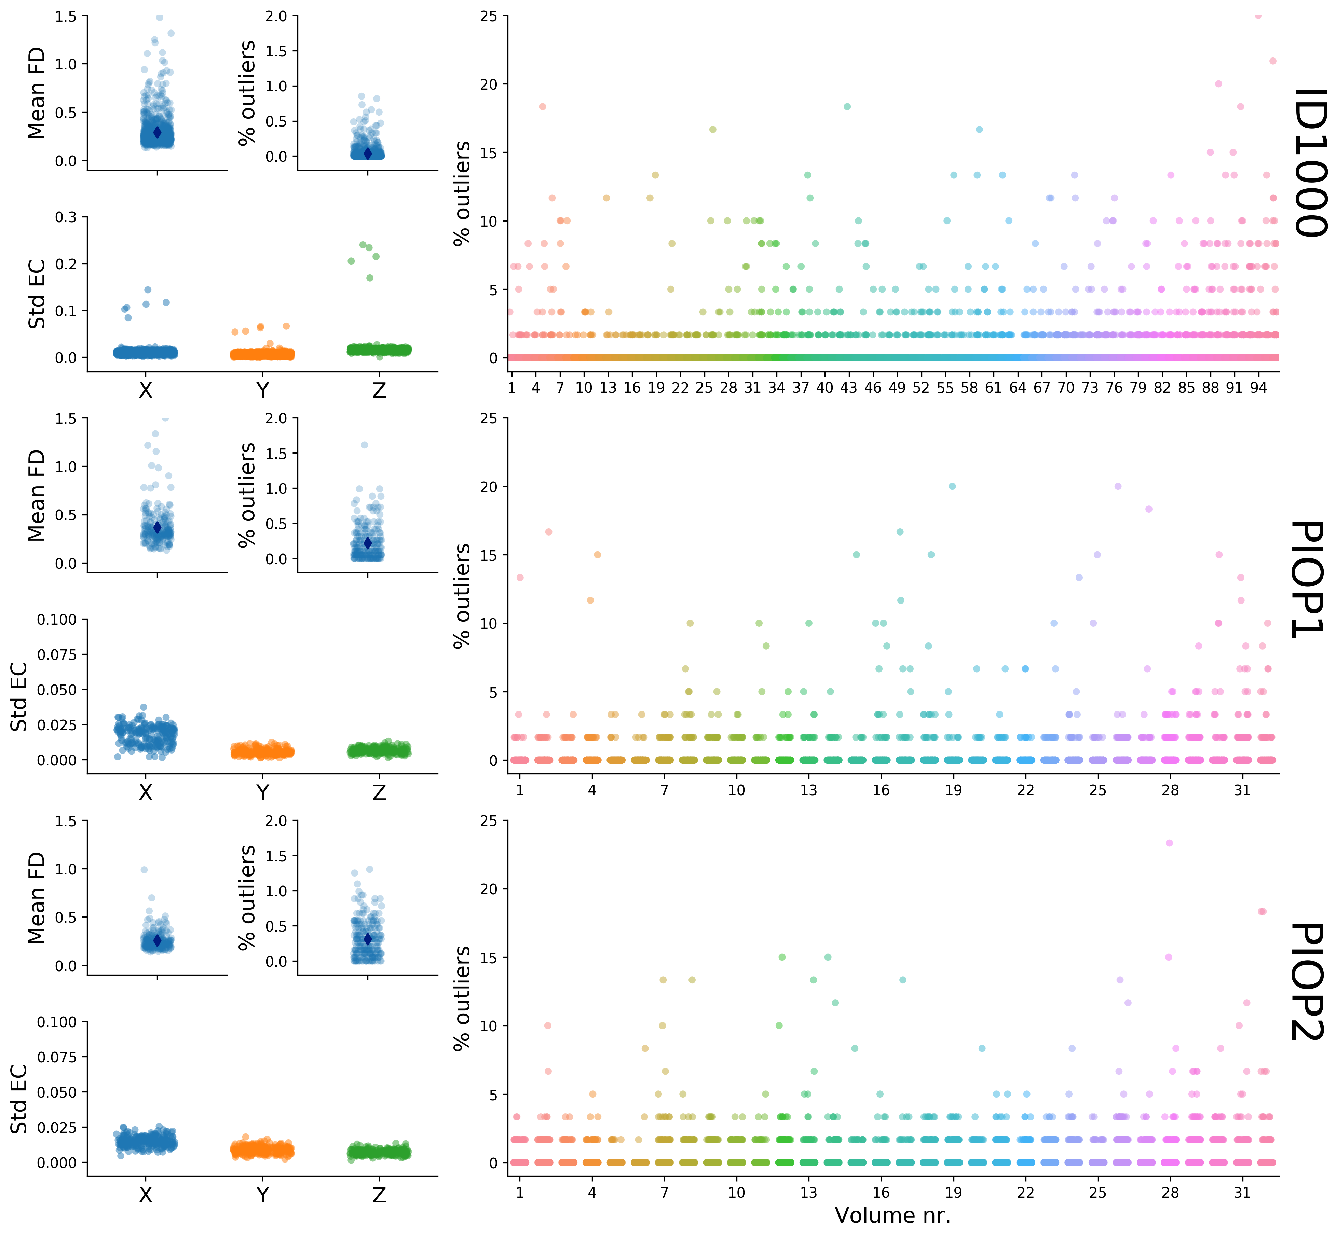
\includegraphics{_bookdown_files/aomic-files/figures/figure_10.pdf}
\caption{\label{fig:fig-aomic-10}Quality control metrics related to the diffusion-weighted scans. FD: framewise displacement, Std EC: standard deviation of the linear terms of the eddy current distortions in Hz/mm.}
\end{figure}



Finally, for each dataset, we transformed all preprocessed DTI eigenvectors to a population template estimated on all FA images using MRTrix' \emph{population\_template} (using a linear followed by a non-linear registration procedure) and computed the voxelwise median across subjects. The median eigenvector images are visualized in Figure \ref{fig:fig-aomic-11} as ``diffusion-encoded color'' (DEC) images, in which values are modulated by the associated FA values.

\begin{figure}
\centering
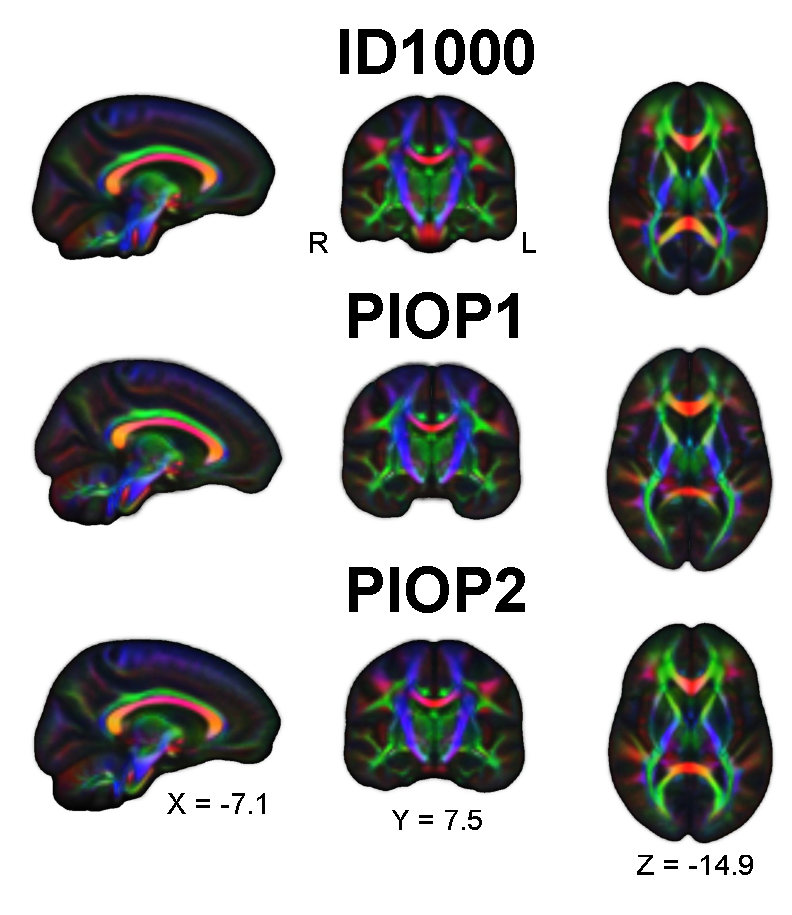
\includegraphics{_bookdown_files/aomic-files/figures/figure_11.pdf}
\caption{\label{fig:fig-aomic-11}Diffusion-encoded color images of the FA-modulated median DTI eigenvectors across subjects. Red colors denote preferential diffusion along the sagittal axis (left-right), green colors denote preferential diffusion along the coronal axis (anterior-posterior), and blue colors denote preferential diffusion along the axial axis (inferior-superior). Brighter colors denote stronger preferential diffusion.}
\end{figure}



\hypertarget{physiological-data}{%
\subsection{Physiological data}\label{physiological-data}}

After conversion to BIDS, physiological data was visually checked for quality by plotting the scanner triggers (i.e., volume onsets) and the cardiac and respiratory traces. Files missing a substantial window of data (\textgreater10 seconds) were excluded as well as files for which the scanner triggers could not be estimated reliably. Figures of the physiology traces and scanner triggers for each file are included in the physiology derivatives. Additionally, using the same approach as described for the task-based technical validation analyses, we fit first-level (subject-specific) and subsequently group-level (subject-average) models using the physiology regressors (all 18 RETROICOR regressors, one HRV, and one RVT regressor) for each dataset. In Figure \ref{fig:fig-aomic-12}, we visualize the effects of the different RETROICOR components (respiratory, cardiac, and interaction regressors; an \emph{F}-test, but converted to and visualized as \emph{z}-scores) and the HRV and RVT regressors (a \emph{t}-test, but converted to and visualized as \emph{z}-scores). Unthresholded whole-brain maps are available from NeuroVault.

\begin{figure}
\centering
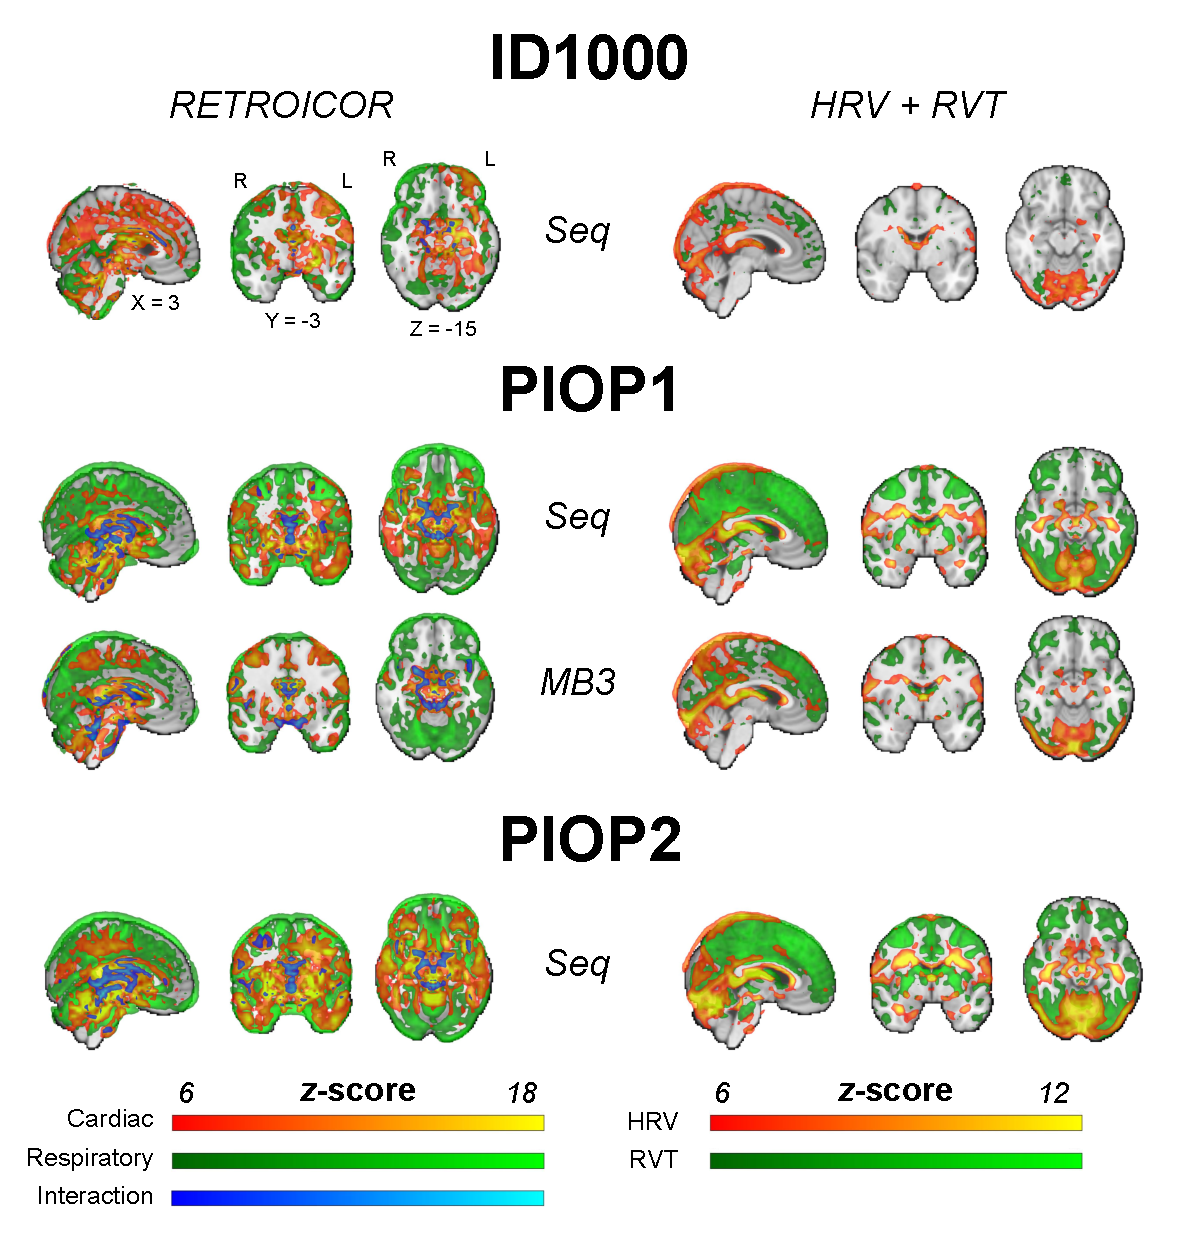
\includegraphics{_bookdown_files/aomic-files/figures/figure_12.pdf}
\caption{\label{fig:fig-aomic-12}Results from group-level physiology analyses. Brain maps show uncorrected effects (thresholded arbitrarily at \emph{z} \textgreater{} 6) and were linearly interpolated for visualization in \emph{FSLeyes}. Unthresholded whole-brain \emph{z}-value maps are available on NeuroVault.}
\end{figure}



\hypertarget{psychometric-data}{%
\subsection{Psychometric data}\label{psychometric-data}}

The patterns of correlations within the scales of the questionnaires are consistent with those reported in literature, indicating that this data is overall reliable. The pattern of correlations between scales of different questionnaires and external variables is also consistent with those reported in literature and what would be expected on theoretical grounds.

\hypertarget{intelligence-structure-test-ist}{%
\subsubsection{Intelligence Structure Test (IST)}\label{intelligence-structure-test-ist}}

The subscales of the IST (fluid and crystallized intelligence and memory) are strongly correlated with each other. The validity of the measure data is supported by the correlation with relevant external variables like educational level, \(r(926) = 0.46\)) and background SES, \(r(926) = 0.35\) (see Table \ref{tab:tab-aomic-6}).

\begingroup\fontsize{8}{10}\selectfont

\begin{ThreePartTable}
\begin{TableNotes}[para]
\item \textit{Note: } 
\item IST: Intelligence Structure Test, Int: Total Intelligence, SES: background social-economic status. ** indicates p < 0.01.
\end{TableNotes}
\begin{longtabu} to \linewidth {>{\raggedright}X>{\raggedleft}X>{\raggedright}X>{\raggedright}X>{\raggedright}X>{\raggedright}X>{\raggedright}X}
\caption{\label{tab:tab-aomic-6}Correlations between total score, and subscales of the IST and relevant external variables.}\\
\toprule
IST (N = 926) & IST Int & IST Crystal & IST Memory & IST Fluid & Background SES & Education\\
\midrule
IST Int & 1 & 0.82** & 0.79** & 0.96** & 0.35** & 0.46**\\
IST Crystallized &  & 1 & 0.58** & 0.68** & 0.37** & 0.44**\\
IST Memory &  &  & 1 & 0.65** & 0.25** & 0.39**\\
IST Fluid &  &  &  & 1 & 0.31** & 0.41**\\
Background SES &  &  &  &  & 1 & 0.38**\\
\addlinespace
Education &  &  &  &  &  & 1\\
\bottomrule
\insertTableNotes
\end{longtabu}
\end{ThreePartTable}
\endgroup{}

\hypertarget{personality-neo-ffi}{%
\subsubsection{Personality: NEO-FFI}\label{personality-neo-ffi}}

The cross-correlation patterns of the five NEO-FFI scales are depicted in Table \ref{tab:tab-aomic-7}. Significant correlations exist between the scales, and the correlation pattern is overall consistent with the reported norm data for this test (Hoekstra et al., \protect\hyperlink{ref-Hoekstra1996-kv}{1996}). The correlation between cross-correlation patterns of the three datasets is very consistent (\(r = 0.88\) between PIOP1 and PIOP2, and on average \(r = 0.74\) between ID1000 and PIOP), with as a notable outlier a negative correlation, \(r(928) = -0.13\), \(p < 0.001\), between extraversion and agreeableness in the ID1000 dataset and a positive correlation for these scales in the PIOP1, \(r(216) = 0.20\), \(p < 0.005\), and PIOP2, \(r(226) = 0.26\), \(p < 0.001\). A source for this discrepancy could be the difference in population sample between the PIOP1 and PIOP2 studies and the ID1000 study.

\begingroup\fontsize{8}{10}\selectfont

\begin{ThreePartTable}
\begin{TableNotes}[para]
\item \textit{Note: } 
\item With the exception of the correlation between agreeableness and extraversion the  cross-correlation patterns are very similar across samples. * indicates p<0.05. ** indicates p<0.01.
\end{TableNotes}
\begin{longtabu} to \linewidth {>{\raggedright}X>{\raggedleft}X>{\raggedright}X>{\raggedright}X>{\raggedright}X>{\raggedright}X}
\caption{\label{tab:tab-aomic-7}Cross-correlations for the subscales of the NEO-FFI for the ID1000, PIOP1 and PIOP2 samples.}\\
\toprule
ID1000 (N = 927) & Neuroticism & Extraversion & Openness & Agreeableness & Conscientiousness\\
\midrule
Neuroticism & 1 & -0.30** & 0.15** & -0.08* & -0.43**\\
Extraversion &  & 1 & 0.20** & -0.13** & 0.12**\\
Openness &  &  & 1 & -0.06 & -0.19**\\
Agreeableness &  &  &  & 1 & 0.16**\\
Conscientiousness &  &  &  &  & \vphantom{2} 1\\
\addlinespace
\textbf{PIOP1 (N = 216)} & \textbf{} & \textbf{} & \textbf{} & \textbf{} & \textbf{}\\
Neuroticism & 1 & -0.29** & 0.18** & 0 & -0.25**\\
Extraversion &  & 1 & -0.05 & 0.20** & 0.14*\\
Openness &  &  & 1 & 0.08 & -0.18**\\
Agreeableness &  &  &  & 1 & 0.20**\\
\addlinespace
Conscientiousness &  &  &  &  & \vphantom{1} 1\\
\textbf{PIOP2 (N = 226)} & \textbf{} & \textbf{} & \textbf{} & \textbf{} & \textbf{}\\
Neuroticism & 1 & -0.38** & 0.12 & -0.07 & -0.24**\\
Extraversion &  & 1 & 0.11 & 0.26** & 0.25**\\
Openness &  &  & 1 & 0.02 & -0.04\\
\addlinespace
Agreeableness &  &  &  & 1 & 0.15*\\
Conscientiousness &  &  &  &  & 1\\
\bottomrule
\insertTableNotes
\end{longtabu}
\end{ThreePartTable}
\endgroup{}

In terms of external validity we note that openness to experience has a positive correlation with intelligence in all three samples (ID1000: \(r(925) = 0.22\), \(p < 0.001\), PIOP1: \(r(216) = 0.25\), \(p = 0.000196\)), PIOP2: \(r(225) = 0.24\), \(p = 0.000276\)).

\hypertarget{bisbas}{%
\subsubsection{BIS/BAS}\label{bisbas}}

The cross-correlation patterns of the BIS/BAS scales are depicted in Table \ref{tab:tab-aomic-8}. The cross-correlation between the scales are similar to the one reported by Franken et al. (\protect\hyperlink{ref-Franken2005-jg}{2005}) and contrary to what Carver \& White (\protect\hyperlink{ref-Carver1994-wp}{1994}) predicted, with a positive correlation between the three different BAS-scales, but also between BIS and BAS-Reward, \(r(927) = 0.194\).

\begingroup\fontsize{8}{10}\selectfont

\begin{ThreePartTable}
\begin{TableNotes}[para]
\item \textit{Note: } 
\item ** indicates p<0.01.
\end{TableNotes}
\begin{longtabu} to \linewidth {>{\raggedright}X>{\raggedleft}X>{\raggedright}X>{\raggedright}X>{\raggedright}X}
\caption{\label{tab:tab-aomic-8}Cross-correlations for the subscales of the BIS/BAS for the ID1000 sample.}\\
\toprule
BIS/BAS (N = 928) & BAS drive & BAS fun & BAS reward & BIS\\
\midrule
BAS drive & 1 & 0.45** & 0.34** & -0.19**\\
BAS fun &  & 1 & 0.39** & -0.13**\\
BAS reward &  &  & 1 & 0.19**\\
BIS &  &  &  & 1\\
\bottomrule
\insertTableNotes
\end{longtabu}
\end{ThreePartTable}
\endgroup{}

\hypertarget{stai-t}{%
\subsubsection{STAI-T}\label{stai-t}}

The STAI-T scale measures trait anxiety. Because this instrument only consists of one scale we evaluate its reliability on the degree in which it shows correlations with other questionnaire scales that also have a pretension of measuring negative emotionality. Because we observe positive correlations with both Neuroticisms, \(r(927) = 0.77\), \(p < 0.001\)) and BIS, \(r(927) = 0.514\), \(p < 0.001\)) we conclude that the reported scales are reliable and consistent.

\hypertarget{aomic-code-availability}{%
\subsection{Code availability}\label{aomic-code-availability}}

All code used for curating, annotating, and (pre)processing AOMIC are version-controlled using git and can be found in project-specific Github repositories within the NILAB-UvA Github organization: \url{https://github.com/orgs/NILAB-UvA}. Many pre and postprocessing steps were identical across datasets, so the code for these procedures is stored in a single repository: \url{https://github.com/NILAB-UvA/AOMIC-common-scripts}. Possible parameters are all hard-coded within the scripts, except for a single positional parameter pointing to the directory to be processed. For custom Python-based scripts, we used Python version 3.7. All code was developed on a Linux system with 56 CPUs (Intel Xeon E5-2680 v4, 2.40GHz) and 126GB RAM running Ubuntu 16.04. All curation, preprocessing, and analyses were run on said Linux system, apart from the \emph{Fmriprep}, \emph{Mriqc}, and \emph{Freesurfer} analyses, which were run in a Docker container provided by those software packages. Custom code was parallelized to run on multiple CPUs concurrently using the Python package \emph{joblib} (\url{https://joblib.readthedocs.io}).

For curation, preprocessing, and analysis of the datasets, we used a combination of existing packages and custom scripts (written in Python or bash). To convert the data to the Brain Imaging Data Structure (\emph{BIDS}), we used the in-house developed, publicly available software package \emph{bidsify} (v0.3; \url{https://github.com/NILAB-UvA/bidsify}), which in turn uses the \emph{dcm2niix} (v1.0.20181125; Li et al., \protect\hyperlink{ref-Li2016-ss}{2016}) to convert the Philips PAR/REC files to compressed nifti files. In contrast to the data from PIOP1 and PIOP2 (which were converted to nifti using \emph{dcm2niix}), \emph{r2aGUI} (v2.7.0; \url{http://r2agui.sourceforge.net}) was used to convert the data from ID1000. Because \emph{r2aGUI} does not correct the gradient table of DWI scans for slice angulation, we used the \emph{angulation\_correction\_Achieva} Matlab script (version December 29, 2007) from Jonathan Farrell to do so (available for posterity at \url{https://github.com/NILAB-UvA/ID1000/blob/master/code/bidsify/DTI_gradient_table_ID1000.m}). To remove facial characteristics from anatomical scans, we used the \emph{pydeface} package (v.1.1.0; Gulban et al., \protect\hyperlink{ref-Gulban2019-sv}{2019}). Finally, to convert the raw physiology files (i.e., Philips ``SCANPHYSLOG'' files) to BIDS, we used the in-house developed, publicly available Python package \emph{scanphyslog2bids} (v0.1; \url{https://github.com/lukassnoek/scanphyslog2bids}). The outputs from the BIDS-conversion pipeline were checked using the \emph{bids-validator} software package (v1.4.3).

Anatomical and functional MRI preprocessing were done using \emph{Fmriprep} (v1.4.1; see the \protect\hyperlink{aomic-derivatives}{Derivatives} section for extensive information about \emph{Fmriprep}'s preprocessing pipeline{]}. For our DWI preprocessing pipeline, we used tools from the MRtrix3 package (www.mrtrix.org; v3.0\_RC3; Tournier et al., \protect\hyperlink{ref-Tournier2019-hh}{2019}) and FSL (v6.0.1; Jenkinson et al., \protect\hyperlink{ref-Jenkinson2012-ui}{2012}). For the VBM and dual regression pipelines, we used \emph{FSL} (v6.0.1; Douaud et al., \protect\hyperlink{ref-Douaud2007-sw}{2007}; Good, Johnsrude, et al., \protect\hyperlink{ref-Good2001-kv}{2001}\protect\hyperlink{ref-Good2001-kv}{b}; Smith et al., \protect\hyperlink{ref-Smith2004-sc}{2004}). To create the files with \emph{Freesurfer}-based metrics across all participants, we used \emph{Freesurfer} version 6.0.095. Physiological nuisance regressors (RETROICOR and HRV/RVT regressors) were estimated using the \emph{TAPAS PhysIO} Matlab package (v3.2.0; Kasper et al., \protect\hyperlink{ref-Kasper2017-lp}{2017}).

First-level functional MRI analyses for technical validation were implemented using the Python package \emph{nistats} (v0.0.1b2; Abraham et al., \protect\hyperlink{ref-Abraham2014-ef}{2014}) and \emph{nilearn} (v0.6.2; Abraham et al., \protect\hyperlink{ref-Abraham2014-ef}{2014}; Pedregosa et al., \protect\hyperlink{ref-pedregosa2011scikit}{2011}). For the inter-subject correlation analysis the \emph{Brain Imaging Analysis Kit} was used (\emph{BrainIAK}, \url{http://brainiak.org}, v0.10; RRID:SCR\_014824; Kumar et al., \protect\hyperlink{ref-Kumar2020-eo}{2020}). Plotting brain images was done using \emph{FSLeyes} (v0.32; McCarthy, \protect\hyperlink{ref-McCarthy2019-yt}{2021}) and plotting statistical plots was done using the Python packages \emph{seaborn} (Waskom et al., \protect\hyperlink{ref-Waskom2020-qq}{2020}) and \emph{Matplotlib} (Hunter, \protect\hyperlink{ref-Hunter2007-at}{2007}).

\hypertarget{morbid-curiosity}{%
\chapter{Choosing to view morbid information involves reward circuitry}\label{morbid-curiosity}}

\chaptermark{Morbid Curiosity}

\vspace*{\fill}

\begin{center}\rule{0.5\linewidth}{0.5pt}\end{center}

\small

\noindent
\emph{This chapter has been published as}: Oosterwijk, S., Snoek, L., Tekoppele, J., Engelbert, L. H., \& Scholte, H. S. (2020). Choosing to view morbid information involves reward circuitry. \emph{Scientific reports, 10}(1), 1-13.

\newpage
\normalsize

\begin{abstract}
People often seek out stories, videos or images that detail death, violence or harm. Considering the ubiquity of this behavior, it is surprising that we know very little about the neural circuits involved in choosing negative information. Using fMRI, the present study shows that choosing intensely negative stimuli engages similar brain regions as those that support extrinsic incentives and ``regular'' curiosity. Participants made choices to view negative and positive images, based on negative (e.g., a soldier kicks a civilian against his head) and positive (e.g., children throw flower petals at a wedding) verbal cues. We hypothesized that the conflicting, but relatively informative act of choosing to view a negative image, resulted in stronger activation of reward circuitry as opposed to the relatively uncomplicated act of choosing to view a positive stimulus. Indeed, as preregistered, we found that choosing negative cues was associated with activation of the striatum, inferior frontal gyrus, anterior insula, and anterior cingulate cortex, both when contrasting against a passive viewing condition, and when contrasting against positive cues. These findings nuance models of decision-making, valuation and curiosity, and are an important starting point when considering the value of seeking out negative content.
\end{abstract} \newpage

\hypertarget{morbid-curiosity-introduction}{%
\section{Introduction}\label{morbid-curiosity-introduction}}

Humans are active agents who often deliberately expose themselves to ``morbid'' information (e.g., information involving death, violence or harm). People choose to watch gruesome documentaries, click on links detailing terrifying attacks and visit locations of horrible events. Surprisingly, the fact that people experience curiosity for negative information, and often act on this feeling, is rarely addressed in theoretical models of curiosity and decision-making. Moreover, empirical work on this phenomenon is markedly limited and studies investigating the neural circuits involved in choosing negative information are virtually non-existent. Nevertheless, ``morbid curiosity'' is an important topic for investigation, because this ubiquitous behavior appears to be at odds with the idea that value and reward drive human information seeking. The present paper aims to expand the scientific inquiry of curiosity and choice, by investigating how the brain, and reward-related brain regions in particular, represent a deliberate choice to view intensely negative images that portray death, violence or harm.

In the last decades, much progress has been made in understanding the neuroscience of choice, valuation and curiosity. Yet, when studying choice, decision-making scientists typically focus on extrinsically rewarding stimuli, such as monetary rewards (Braver et al., \protect\hyperlink{ref-braver2014mechanisms}{2014}). Decisions regarding intrinsically rewarding stimuli are targeted less frequently (Murayama, \protect\hyperlink{ref-murayama2018psychological}{2018}) and even less is known about the neural representation of seeking negative information that, at first glance, does not seem to have reward value at all (Elliot, \protect\hyperlink{ref-elliot2006hierarchical}{2006}). Similarly, in the field of curiosity --- defined as an intrinsically motivated drive state for information (Golman \& Loewenstein, \protect\hyperlink{ref-golman2015curiosity}{2015}; Gottlieb et al., \protect\hyperlink{ref-gottlieb2013information}{2013}; Kidd \& Hayden, \protect\hyperlink{ref-kidd2015psychology}{2015}) --- research on curiosity for negative information is scarce (Murayama, \protect\hyperlink{ref-murayama2018psychological}{2018}; see for exceptions Oosterwijk, \protect\hyperlink{ref-oosterwijk2017choosing}{2017}\protect\hyperlink{ref-oosterwijk2017choosing}{a}; Hsee \& Ruan, \protect\hyperlink{ref-hsee2016pandora}{2016}; Rimé et al., \protect\hyperlink{ref-rime2005brief}{2005}; Zuckerman \& Litle, \protect\hyperlink{ref-zuckerman1986personality}{1986}). A handful of neuroscience studies have demonstrated that curiosity engages similar neural circuits as extrinsic reward, but only when examining positive or neutral material, such as trivia questions (e.g., Gruber et al., \protect\hyperlink{ref-gruber2014states}{2014}; Kang et al., \protect\hyperlink{ref-kang2009wick}{2009}). At present, it is thus unclear whether curiosity for ``morbid'' information is supported by similar neural mechanisms as those that support extrinsic incentives and ``regular'' curiosity.

Neuroscientific evidence suggests that curiosity, choice and reward are supported by a highly similar constellation of brain regions4,13. Reward-related decision making, predominantly studied by focusing on monetary gains or losses, engages the dorsal striatum (caudate, putamen), ventral striatum (NAcc), orbitofrontal cortex (OFC), bilateral anterior insula, anterior cingulate cortex (ACC), dorsomedial prefrontal cortex/supplementary motor area (dmPFC/SMA) and frontal and parietal regions often associated with cognitive control14,15,16,17,18. Several studies targeting curiosity demonstrated similar neural regions. For example, Kang and colleagues12 found increased activation in the inferior frontal gyrus (IFG), caudate and putamen when inducing curiosity by presenting trivia questions. When curiosity was relieved (i.e., when the answer to the question was given) they found engagement of the putamen and IFG. In another study targeting trivia questions, Gruber and colleagues11 found increased activation in the dorsal and ventral striatum and IFG for questions associated with high curiosity ratings. Other work has shown that the induction and relief of curiosity engages regions that are associated with salience detection and uncertainty19,20, including the anterior insula and ACC21,22. In short, the limited work on curiosity so far, demonstrates that curiosity for relatively positive and neutral material engages neural regions that are also recruited during the computation of value and the anticipation of reward. Whether these regions also engage when people act on their curiosity for negatively valenced information is currently unknown.

Neuroscientific evidence suggests that curiosity, choice and reward are supported by a highly similar constellation of brain regions (Kidd \& Hayden, \protect\hyperlink{ref-kidd2015psychology}{2015}; Sakaki et al., \protect\hyperlink{ref-sakaki2018curiosity}{2018}). Reward-related decision making, predominantly studied by focusing on monetary gains or losses, engages the dorsal striatum (caudate, putamen), ventral striatum (NAcc), orbitofrontal cortex (OFC), bilateral anterior insula, anterior cingulate cortex (ACC), dorsomedial prefrontal cortex/supplementary motor area (dmPFC/SMA) and frontal and parietal regions often associated with cognitive control (Bartra et al., \protect\hyperlink{ref-bartra2013valuation}{2013}; Diekhof et al., \protect\hyperlink{ref-diekhof2012role}{2012}; Levy \& Glimcher, \protect\hyperlink{ref-levy2012root}{2012}; Liu et al., \protect\hyperlink{ref-liu2011common}{2011}; Samanez-Larkin \& Knutson, \protect\hyperlink{ref-samanez2015decision}{2015}). Several studies targeting curiosity demonstrated similar neural regions. For example, Kang et al. (\protect\hyperlink{ref-kang2009wick}{2009}) found increased activation in the inferior frontal gyrus (IFG), caudate and putamen when inducing curiosity by presenting trivia questions. When curiosity was relieved (i.e., when the answer to the question was given) they found engagement of the putamen and IFG. In another study targeting trivia questions, Gruber et al. (\protect\hyperlink{ref-gruber2014states}{2014}) found increased activation in the dorsal and ventral striatum and IFG for questions associated with high curiosity ratings. Other work has shown that the induction and relief of curiosity engages regions that are associated with salience detection and uncertainty (Menon \& Uddin, \protect\hyperlink{ref-menon2010saliency}{2010}; Singer et al., \protect\hyperlink{ref-singer2009common}{2009}), including the anterior insula and ACC (Jepma et al., \protect\hyperlink{ref-jepma2012neural}{2012}; Lieshout et al., \protect\hyperlink{ref-van2018induction}{2018}). In short, the limited work on curiosity so far, demonstrates that curiosity for relatively positive and neutral material engages neural regions that are also recruited during the computation of value and the anticipation of reward. Whether these regions also engage when people act on their curiosity for negatively valenced information is currently unknown.

In the present study, we tested the preregistered hypothesis that the striatum and IFG (ROI-analyses) and the anterior insula and ACC (whole-brain analyses) will engage more when people deliberately choose to view negative images, as compared to a passive viewing condition. This hypothesis reflects our assumption that ``morbid curiosity'', expressed by a choice to view a negative stimulus, engages similar neural regions as regular curiosity (Gruber et al., \protect\hyperlink{ref-gruber2014states}{2014}; Jepma et al., \protect\hyperlink{ref-jepma2012neural}{2012}; Kang et al., \protect\hyperlink{ref-kang2009wick}{2009}; Lieshout et al., \protect\hyperlink{ref-van2018induction}{2018}; see for an overview Gruber \& Ranganath, \protect\hyperlink{ref-gruber2019curiosity}{2019}). In addition, we tested a second hypothesis that the regions described above will engage more strongly when people choose to view a negative stimulus, as compared to a positive stimulus. This hypothesis is based on our assumption that the informational value of negative images is relatively high. Compared to positive information, negative information may be more novel, rare, deviant, uncertain, challenging or complex (Baumeister et al., \protect\hyperlink{ref-baumeister2001bad}{2001}; Unkelbach et al., \protect\hyperlink{ref-unkelbach2008positive}{2008}) --- these information characteristics engage reward circuitry and evoke curiosity (Berlyne, \protect\hyperlink{ref-berlyne1966curiosity}{1966}; Kashdan \& Silvia, \protect\hyperlink{ref-kashdan2009curiosity}{2009}; Kidd \& Hayden, \protect\hyperlink{ref-kidd2015psychology}{2015}; Sakaki et al., \protect\hyperlink{ref-sakaki2018curiosity}{2018}). Furthermore, a choice for negativity may involve a tradeoff between benefits (e.g., understanding something complex) and costs (e.g., being emotionally perturbed by a stimulus). Choosing a positive stimulus (e.g., viewing a family picnicking in the park) may not involve such costs, and may also have less benefits in terms of accessing novel, deviant or complex information. In this sense, choosing negativity (or ``morbid curiosity'') is a conflict state; people want information, without predicting that they will like the information (see also Rimé et al., \protect\hyperlink{ref-rime2005brief}{2005}; Litman, \protect\hyperlink{ref-litman2005curiosity}{2005}). Previous work suggests that reward circuitry engagement is most pronounced when actions or decisions are ambiguous or unclear (Floresco, \protect\hyperlink{ref-floresco2015nucleus}{2015}). In line with this, we predict that the conflicting, but relatively informative act of choosing to view a negative image will paradoxically result in stronger activation of reward circuitry as opposed to the relatively uncomplicated act of choosing to view a positive stimulus.

We build upon previous work that demonstrates that people are interested in and fascinated by negative images (Oosterwijk et al., \protect\hyperlink{ref-oosterwijk2016neural}{2016}; Oosterwijk, \protect\hyperlink{ref-oosterwijk2017choosing}{2017}\protect\hyperlink{ref-oosterwijk2017choosing}{a}). The present study specifically targets choice for social negative images (i.e., displaying death, violence or harm within a social context), because we found in previous research that people prefer to view these stimuli over neutral alternatives and choose to view these stimuli more often than images of attacking animals and graphic, decontextualized mutilation (Oosterwijk, \protect\hyperlink{ref-oosterwijk2017choosing}{2017}\protect\hyperlink{ref-oosterwijk2017choosing}{a}). We used an established choice paradigm (Oosterwijk, \protect\hyperlink{ref-oosterwijk2017choosing}{2017}\protect\hyperlink{ref-oosterwijk2017choosing}{a}) that presented participants with choices to view social images that depicted negative and positive situations, taken from validated affective picture databases. Importantly, this paradigm solely targets intrinsic motivation; participants were not financially rewarded for their choices. Moreover, this paradigm targets a behavioral expression of ``wanting'', and not the extent to which people ``like'' the images (Berridge et al., \protect\hyperlink{ref-berridge2009dissecting}{2009}; Litman, \protect\hyperlink{ref-litman2005curiosity}{2005}). The active-choice condition was compared to a passive-viewing condition, using a yoked procedure that has been previously used to study responses to controllable and incontrollable stressors (Amat et al., \protect\hyperlink{ref-amat2005medial}{2005}; Wood et al., \protect\hyperlink{ref-wood2015controllability}{2015}). In the present study, a yoked design allowed us to investigate the effect of choice, while controlling for general affective, semantic and visual processing.

In the choice condition, people were presented with verbal cues, describing negative images (e.g., a soldier kicks a civilian against his head) and positive images (e.g., children throw flower petals at a wedding). The presentation of the verbal cue was labeled the induction phase (see Figure \ref{fig:fig-morbid-curiosity-1}). Following the cue, participants chose whether they wanted to see the image corresponding to the description, or not. In the relief phase (see Figure \ref{fig:fig-morbid-curiosity-1}), participants viewed the corresponding image when responding yes and a blurred version when responding no. The passive-viewing condition was fully yoked to the active-choice condition. In other words, each participant in the passive-viewing condition did not make choices, but was confronted with the choice profile of a participant in the active-choice condition. Importantly, this yoked design isolates the psychological process that we aim to investigate (i.e., a deliberate choice to view a stimulus), while keeping all other factors constant (i.e., cues and images). In line with curiosity theories that argue that exploratory behavior is an important component of curiosity (Kashdan \& Silvia, \protect\hyperlink{ref-kashdan2009curiosity}{2009}; Litman, \protect\hyperlink{ref-litman2005curiosity}{2005}; Loewenstein, \protect\hyperlink{ref-loewenstein1994psychology}{1994}), we propose that the potential to choose will make participants' subjective experience of curiosity more salient. In other words, participants' subjective state of curiosity may be more at the fore-front of consciousness in the active-choice condition (because it will inform participants' decisions) than in the passive-viewing condition.

\begin{figure}
\centering
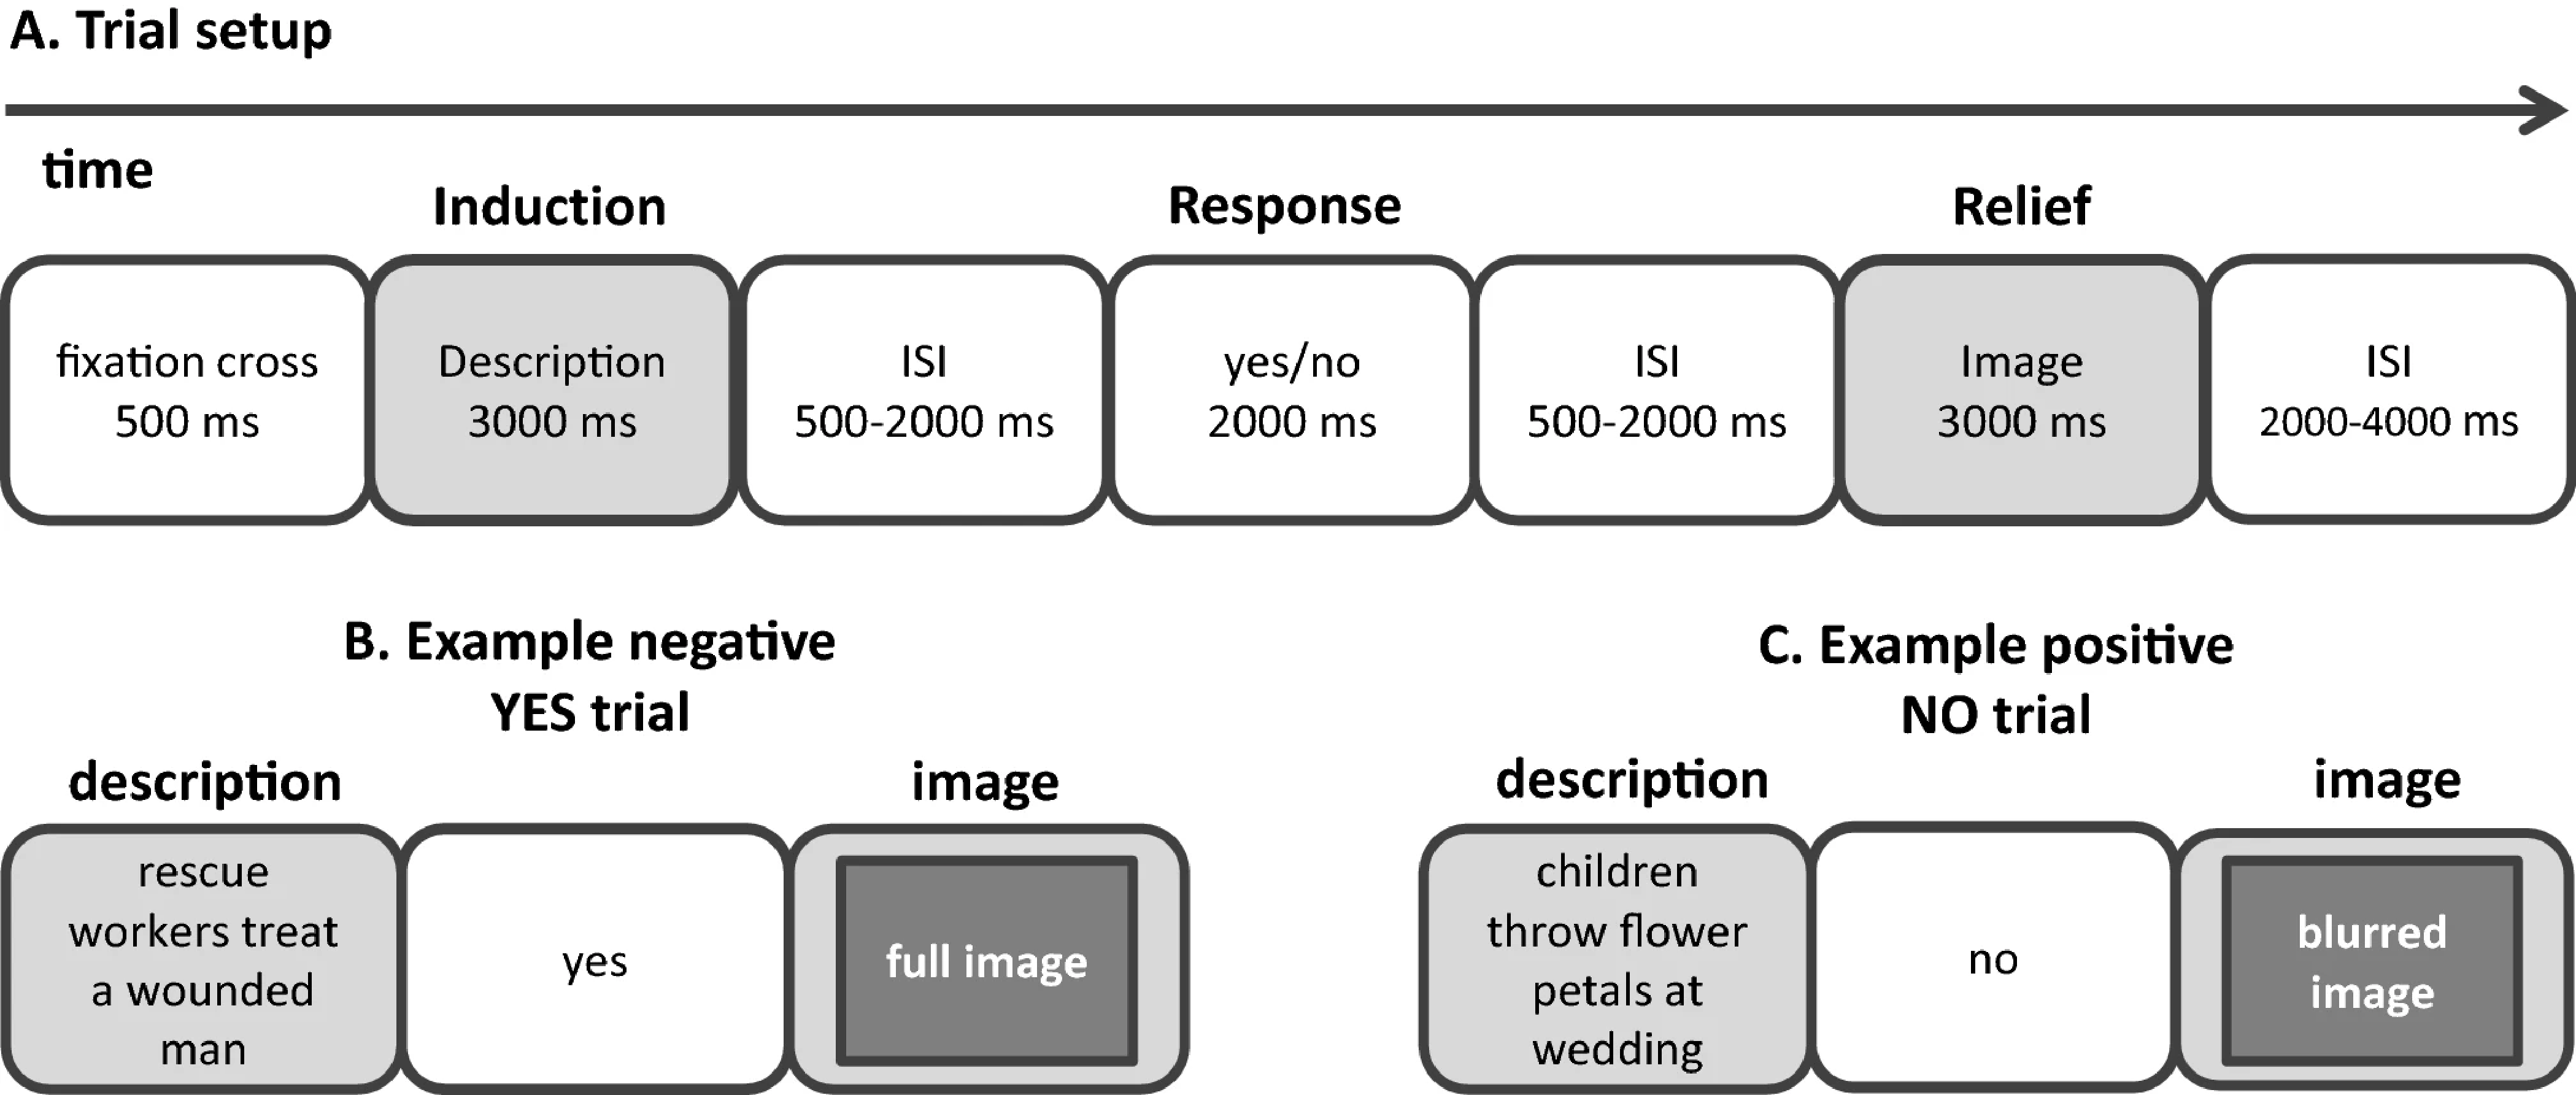
\includegraphics{_bookdown_files/morbid-curiosity-files/figures/figure_1.pdf}
\caption{\label{fig:fig-morbid-curiosity-1}Overview of paradigm. (\textbf{A}) The setup of the trials in the choice-condition and passive-viewing condition. Note that in the active-choice condition, participants chose whether they wanted to see the image corresponding to the description during the yes/no response event. In the passive-viewing condition participants did not choose, but confirmed the decision seemingly determined by the computer during the yes/no response event. (\textbf{B}) An example of a negative description and the consequence of a yes response (either given by the participant, or determined by the computer). (\textbf{C}) An example of a positive description and the consequence of a no response (either given by the participant, or determined by the computer).}
\end{figure}



We selected positive and negative images from the International Affective Picture System database (Lang et al., \protect\hyperlink{ref-lang1997international}{1997}) and the Nencki Affective Picture System database (Marchewka et al., \protect\hyperlink{ref-marchewka2014nencki}{2014}). Importantly, we matched negative and positive images in terms of valence extremity to ensure that, on average, positive images were perceived as equally positive as negative stimuli were perceived negative. A similar procedure was performed for the positive and negative descriptions (i.e., cues; see \protect\hyperlink{morbid-curiosity-methods}{Methods} section for further details).

Our scanning protocol was performed on a 3 T scanner. For all details on image acquisition, preprocessing and first- and second-level analyses, please see the \protect\hyperlink{morbid-curiosity-methods}{Methods} section. Our analysis protocol held confirmatory and exploratory analyses. Hypotheses and corresponding contrasts for the confirmatory analyses, exclusion criteria, ROIs and corrections for multiple comparisons were preregistered on the Open Science Framework, prior to data analysis (\url{osf.io/gdtk9}; Oosterwijk, \protect\hyperlink{ref-oosterwijk2017prereg}{2017}\protect\hyperlink{ref-oosterwijk2017prereg}{b}).

The first-level model included six predictors to capture the research design: 2 (phase: induction phase vs.~relief phase) × 2 (valence: negative vs.~positive) × 2 (choice: yes, full image vs.~no, blurred image). Additionally, we added a single predictor for the motor response associated with the decision/confirmation response and six motion predictors based on estimated motion correction parameters. First level contrasts only involved trials associated with yes choices (i.e., full image trials); trials associated with no responses (i.e., blurred image trials) were not used for further group level analysis.

In the ROI-based analyses, we focused on voxels within two a-priori defined ROIs: bilateral striatum and bilateral inferior frontal gyrus (IFG). The ROIs were based on the Harvard-Oxford Subcortical Atlas (striatum; caudate, putamen and nucleus accumbens) and the Harvard-Oxford Cortical Atlas (IFG; pars opercularis and pars triangularis) with a threshold for probabilistic ROIs \textgreater{} 0 (Craddock et al., \protect\hyperlink{ref-craddock2012whole}{2012}). In the group-level analyses targeting these two ROIs, we calculated two contrasts that reflected our confirmatory hypotheses, separately for the induction and relief phase. We hypothesized stronger activation in the ROIs when participants processed a negative cue/image in the active-choice condition as compared to that same event in the passive-viewing condition (i.e., \((\beta_{\mathrm{neg|active}} -\beta_{\mathrm{neg|passive}}) > 0\)). In addition, we hypothesized stronger activation in the ROIs when participants processed a negative cue/image in the active-choice condition as compared to a positive cue/image in the active-choice condition, controlling for passive viewing (i.e., \((\beta_{\mathrm{neg|active}} - \beta_{\mathrm{neg|active}}) - (\beta_{\mathrm{pos|active}} - \beta_{\mathrm{pos|passive}}) > 0\)). For these confirmatory ROI analyses, we used nonparametric permutation-based inference in combination with Threshold-Free Cluster Enhancement (TFCE; Smith \& Nichols, \protect\hyperlink{ref-smith2009threshold}{2009}) as implemented in \emph{FSL randomise} (Winkler et al., \protect\hyperlink{ref-winkler2014permutation}{2014}) and thresholded voxelwise results at \(p < 0.025\) (correction for two ROIs). Note that this analysis allows for voxel-wise inference (i.e., no cluster-based correction is used). In addition to the confirmatory ROI analysis, we conducted an exploratory whole-brain group-level analysis. In addition to the two confirmatory contrasts mentioned in the previous section, we tested three exploratory contrasts, separately for the induction and relief phase with a voxel-wise \emph{p}-value threshold of 0.005 and a cluster-wise \emph{p}-value of 0.05). Full details regarding the exploratory analyses can be found in the \protect\hyperlink{morbid-curiosity-methods}{Methods} section.

\hypertarget{morbid-curiosity-methods}{%
\section{Methods}\label{morbid-curiosity-methods}}

\hypertarget{morbid-curiosity-methods-participants}{%
\subsection{Participants}\label{morbid-curiosity-methods-participants}}

Participants consisted of a convenience sample of students at the University of Amsterdam. The study was approved by the Ethics Review Board of the department of Psychology at the University of Amsterdam (2017-SP-7871) and performed in accordance with relevant institutional guidelines. The budget allowed for scanning of a maximum of 60 participants. After applying the exclusion criteria, the total sample consisted of 54 participants, including 38 women (\emph{M\textsubscript{age}} = 22.4, \emph{SD} = 2.9) and 16 men (\emph{M\textsubscript{age}} = 23.8, \emph{SD} = 1.8).

\hypertarget{morbid-curiosity-methods-design}{%
\subsection{Design}\label{morbid-curiosity-methods-design}}

This study used a 2 (choice: active-choice vs.~passive-viewing) × 2 (phase: induction vs.~relief) × 2 (valence: negative vs.~positive) mixed design. The variable choice was varied between participants and consisted of an active-choice condition and a passive-viewing condition. The variable phase was varied within participants and reflected the presentation of the cue (i.e., induction) vs.~the presentation of the image (i.e., relief). The variable valence was varied within participants and reflected the negative vs.~positive content of the cues/images.

\hypertarget{morbid-curiosity-methods-materials}{%
\subsection{Materials}\label{morbid-curiosity-methods-materials}}

\hypertarget{morbid-curiosity-methods-materials-experimental-task}{%
\subsubsection{Experimental task}\label{morbid-curiosity-methods-materials-experimental-task}}

The present study utilized a choice task (Oosterwijk, \protect\hyperlink{ref-oosterwijk2017choosing}{2017}\protect\hyperlink{ref-oosterwijk2017choosing}{a}) that presented participants with verbal cues describing negative and positive images, and offered them a choice to see these images or blurred versions. We used a yoked design that isolated the effects of choice, controlling for general affective, semantic and visual processing (see also Wood et al., \protect\hyperlink{ref-wood2015controllability}{2015}; Amat et al., \protect\hyperlink{ref-amat2005medial}{2005}). This yoked design resulted in two conditions: the active-choice condition and the passive-viewing condition. Participant in the passive-viewing condition did not make choices, but were confronted with the choice profile of a yoked participant in the choice condition. Tasks in both conditions were programmed in Neurobs Presentation (\url{https://www.neurobs.com/presentation}). Behavioral data preprocessing was done using Python 3.5 and analyzed using IBM SPSS Statistics 22.0.

In the active-choice condition, participants were presented with 35 negative cues (e.g., rescue workers treat a wounded man; a soldier kicks a civilian against his head) and 35 positive cues (e.g., children throw flower petals at a wedding; partying people carry a crowd surfer) that described images, in random order. In each trial participants could choose, based on the cue, whether they wanted to view the corresponding image or not. The choice task consisted of a total of 70 trials. Each trial started with a fixation cross, presented for 500 ms, followed by the cue, presented for 3,000 ms. The presentation of the cue was labelled as the induction phase (see also Jepma et al., \protect\hyperlink{ref-jepma2012neural}{2012}; Lieshout et al., \protect\hyperlink{ref-van2018induction}{2018}). The cue was followed by a jittered interval varying between 500 and 2000 ms. Subsequently, participants saw the words `yes' and `no' on the screen, and chose whether they wanted to see the image that was described by the cue, or not, by pressing one of two pre-specified buttons. Immediately following their response, the word `yes' or `no' turned green, indicating that their response was registered. Participants had a 2000 ms. time window to make their choice. If they had not made a choice after 2000 ms, the choice was automatically set to `no'. The response phase was followed by a jittered interval varying between 500 and 2000 ms. The interval was followed by the relief phase, in which the participants were presented with the image (1,024 × 768 pixels) when they chose `yes'. When participants chose not to see the corresponding image, they were presented with a blurred version of the image that was unrecognizably distorted (filter). Images were blurred with the software IrfanView (version 4.44; \url{https://www.irfanview.com/}) using the fast Gaussian blur (filter = 150 pixels). Both the image and the blurred image were presented for 3,000 ms. The relief phase was followed by a jittered inter-trial-interval varying between 2000 and 4,000 ms. For a visual representation of the paradigm, please see Figure \ref{fig:fig-morbid-curiosity-1}.

In the passive-viewing condition, participants were presented with the choice profile of a participant in the active-choice condition (i.e., the exact pattern of `yes' and `no' responses to the positive and negative cues for each participant in the active-choice condition was saved, and then re-used once as the computer generated pre-determined choice pattern for a participant in the passive-viewing condition). Participants were told in the introduction to the study that the computer would determine which images would be shown. The trial setup was identical to the active-choice condition, except for the following aspect. After participants were presented with the cue, the word `yes' or `no' turned green, indicating the choice of the computer. Participants were asked to confirm the choice made by the computer by pressing one of two pre-specified buttons, to mirror the motor response made in the active-choice condition.

The active-choice condition came with a filling problem: because participants could choose whether they wanted to view an image or not, some participants would see many more images than others. This filling problem can pose problems for modelling the BOLD response, due to lower efficiency in estimating contrasts for one subject over the other. Based on individual differences in choosing to view social negative information (Oosterwijk, \protect\hyperlink{ref-oosterwijk2017choosing}{2017}\protect\hyperlink{ref-oosterwijk2017choosing}{a}), we formulated an a-priori defined and preregistered eligibility criterion that only participants in the active-choice condition who chose negative and/or positive images in 40\% or more of the trials (14/35 stimuli) would be paired with a subject in the passive-viewing condition. Based on this criterion five out of 33 participants in the active-choice condition were excluded from the sample. One other participant was excluded, because the functional scan was stopped prematurely. This resulted in 27 participants in the active-choice condition. The choice profiles of these 27 participants were yoked with 27 participants in the passive-viewing condition.

\hypertarget{morbid-curiosity-methods-materials-cues}{%
\subsubsection{Cues}\label{morbid-curiosity-methods-materials-cues}}

Cues were written to describe positive and negative images in one sentence. In a pilot study the cues were rated on valence (0 = negative to 100 = positive), and arousal (0 = low arousal to 100 = high arousal). Negative cues were rated more negatively than positive cues (\emph{M} = 20.69, \emph{SD} = 8.42 vs.~\emph{M} = 77.99, \emph{SD} = 4.49), \emph{t}(68) = −35.51, \emph{p} \textless{} 0.001, and more arousing than positive cues (\emph{M} = 68.45, \emph{SD} = 6.38 vs.~\emph{M} = 28.93, \emph{SD} = 5.99), \emph{t}(68) = 26.71, \emph{p} \textless{} 0.001. Negative and positive cues were matched in terms of valence extremity. An analysis of mean-centered valence scores demonstrated that, on average, positive cues were perceived as equally positive (\emph{M} = 29.31, \emph{SD} = 8.43) as negative stimuli were perceived as negative (\emph{M} = 27.99, \emph{SD} = 4.49), \emph{t}(68) = 0.82, \emph{p} = 0.417.

\hypertarget{morbid-curiosity-methods-materials-images}{%
\subsubsection{Images}\label{morbid-curiosity-methods-materials-images}}

Images were selected from the International Affective Picture System (IAPS; Lang et al., \protect\hyperlink{ref-lang1997international}{1997}) and the Nencki Affective Picture System (NAPS; Marchewka et al., \protect\hyperlink{ref-marchewka2014nencki}{2014}); image codes are presented in the \protect\hyperlink{morbid-curiosity-supplement}{Supplementary Materials} (Table \ref{tab:tab-morbid-curiosity-S4}). We selected negative images that portrayed situations of interpersonal violence, or social scenes involving a dead body or a harmed person. Negative images were selected when they had a valence rating below 4 (on a scale from 1 = negative to 9 = positive) and an arousal rating above 4.5 (on a scale from 1 = not arousing to 9 = extremely arousing). We selected positive images that portrayed joyful, loving or exciting interpersonal interactions. Positive images were selected when they had a valence rating above 6 (on a scale from 1 = negative to 9 = positive) and an arousal rating above 3 (on a scale from 1 = not arousing to 9 = extremely arousing). Negative and positive images differed significantly in terms of valence (\emph{M} = 2.58, \emph{SD} = 0.53 vs.~\emph{M} = 7.43, \emph{SD} = 0.36), \emph{t}(68) = −44.88, \emph{p} \textless{} 0.001, and arousal (\emph{M} = 6.18, \emph{SD} = 0.75 vs.~\emph{M} = 4.78, \emph{SD} = 0.90), \emph{t}(68) = 7.07, \emph{p} \textless{} 0.001. Negative and positive images were matched in terms of valence extremity. An analysis of mean-centered valence scores demonstrated that, on average, positive images were perceived as equally positive (\emph{M} = 2.42, \emph{SD} = 0.53) as negative stimuli were perceived as negative (\emph{M} = 2.44, \emph{SD} = 0.37), \emph{t}(68) = − 0.22, \emph{p} = 0.824.

\hypertarget{morbid-curiosity-methods-materials-questionnaires}{%
\subsubsection{Questionnaires}\label{morbid-curiosity-methods-materials-questionnaires}}

After the scanning session was completed, participants filled in the `Morbid curiosity in daily-life' questionnaire (Oosterwijk, \protect\hyperlink{ref-oosterwijk2017choosing}{2017}\protect\hyperlink{ref-oosterwijk2017choosing}{a}) and the Dutch version of the Interpersonal Reactivity Index (De Corte et al., \protect\hyperlink{ref-de2007measuring}{2007}). A short exit questionnaire asked participants two questions regarding the task they performed in the scanner. Participants in the active-choice condition were asked to rate to what extent they followed their curiosity when making choices for negative cues, and when making choices for positive cues, on a 1 (not at all) to 7 (very much) point scale. Participants in the passive-viewing condition were asked to rate to what extent they were curious about the negative cues, and the positive cues, on a 1 (not at all) to 7 (very much) point scale. The exit questionnaire concluded with demographic questions.

\hypertarget{morbid-curiosity-methods-procedure}{%
\subsection{Procedure}\label{morbid-curiosity-methods-procedure}}

After signing the informed consent form, each participant received a thorough instruction. The active-choice condition was introduced as a study on how the brain represents choice. Participants were explained how they could make their choice, that they would always see the image of their choice, and that there were no right or wrong answers. Furthermore, participants were presented with an example of a negative and a positive cue, combined with the corresponding full image and blurred image, so that they knew what to expect when choosing the yes or no option. No mention was made of curiosity in the instruction. The passive-viewing condition was introduced as a study on the brain processes involved in reading image descriptions and viewing images. Participants were explained that the computer determined whether a description would be followed by a corresponding image. As in the active-choice condition, participants were presented with an example of a negative and a positive cue, combined with the corresponding full image and blurred image, so that they knew what to expect when the computer determined the yes or no option.

When comfortable and instructed, a structural T1-weighted anatomical scan was made. Then the participant performed the choice task or the passive task during fMRI acquisition in the scanner. After the scanning session, the participant filled in the questionnaires and received a thorough debriefing.

\hypertarget{morbid-curiosity-methods-behavioral-analysis}{%
\subsection{Behavioral analysis}\label{morbid-curiosity-methods-behavioral-analysis}}

In the active-choice condition, we compared the extent to which participants followed their curiosity when making choices for negative cues and positive cues. In the passive-viewing condition, we compared the extent to which participants were curious about negative cues and positive cues. For the active-choice condition, a Kolmogorov--Smirnov test indicated a normality violation (active-choice: skewness = 0.640, kurtosis = − 0.375, \emph{D}(25) = 0.197, \emph{p} = 0.013; passive-viewing: skewness = − 0.399, kurtosis = − 0.055, \emph{D}(27) = 0.161, \emph{p} = 0.071). We report two paired sample \emph{t}-tests (two-tailed) to analyze the difference between cues, but results were fully corroborated with non-parametric Wilcoxon signed-rank tests. Effect sizes (Cohen's \emph{d\textsubscript{z}}) were calculated using Lakens' (Lakens, \protect\hyperlink{ref-lakens2013calculating}{2013}) spreadsheet.

\hypertarget{morbid-curiosity-methods-imaging-details}{%
\subsection{Imaging details}\label{morbid-curiosity-methods-imaging-details}}

\hypertarget{morbid-curiosity-methods-imaging-details-image-acquisition}{%
\subsubsection{Image acquisition}\label{morbid-curiosity-methods-imaging-details-image-acquisition}}

Participants were tested using a Philips Achieva 3T MRI scanner and a 32-channel SENSE headcoil. A survey scan was made for spatial planning of the subsequent scans. Following the survey scan, a 3-min structural T1-weighted scan was acquired using 3D fast field echo (TR: 82 ms, TE: 38 ms, flip angle: 8°, FOV: 240 × 188 mm, in-plane resolution 240 × 188, 220 slices acquired using single-shot ascending slice order and a voxel size of 1.0 × 1.0 × 1.0 mm). After the T1-weighted scan, functional T2*-weighted sequences were acquired using single shot gradient echo, echo planar imaging (TR = 2000 ms, TE = 27.63 ms, flip angle: 76.1°, FOV: 240 × 240 mm, in-plane resolution 64 × 64, 37 slices with ascending acquisition, slice thickness 3 mm, slice gap 0.3 mm, voxel size 3 × 3 × 3 mm), covering the entire brain. For the functional run, 495 volumes were acquired. After the functional run, a ``B0'' fieldmap scan (based on the phase difference between two consecutive echos) was acquired using 3D fast field echo (TR: 11 ms, TE: 3 ms and 8 ms, flip angle: 8°, FOV: 256 × 208, in-plane resolution 128 × 104, 128 slices).

\hypertarget{morbid-curiosity-methods-imaging-details-preprocessing}{%
\subsubsection{Preprocessing}\label{morbid-curiosity-methods-imaging-details-preprocessing}}

Results included in this manuscript come from preprocessing performed using \emph{FMRIPREP} version 1.0.0 (O. Esteban, Markiewicz, Blair, Moodie, Isik, Erramuzpe, Kent, Goncalves, DuPre, Snyder, \& others, \protect\hyperlink{ref-esteban2019fmriprep}{2019}; O. Esteban, Blair, et al., \protect\hyperlink{ref-esteban_oscar_2017_1095198}{2017}), a \emph{Nipype} (Gorgolewski et al., \protect\hyperlink{ref-Gorgolewski2011-aa}{2011}, \protect\hyperlink{ref-gorgolewski_krzysztof_j_2017_581704}{2017}) based tool. Each T1 weighted volume was corrected for bias field using \emph{N4BiasFieldCorrection} v2.1.0 (Tustison et al., \protect\hyperlink{ref-Tustison2010-tk}{2010}) and skullstripped using \emph{antsBrainExtraction.sh} v2.1.0 (using OASIS template). Cortical surface was estimated using \emph{FreeSurfer} v6.0.0 (Dale et al., \protect\hyperlink{ref-Dale1999-rk}{1999}). The skullstripped T1w volume was segmented (using \emph{FSL FAST}; Zhang et al., \protect\hyperlink{ref-Zhang2001-wa}{2001}) and coregistered to the skullstripped ICBM 152 Nonlinear Asymmetrical template version 2009c (Fonov et al., \protect\hyperlink{ref-Fonov2009-sr}{2009}) using nonlinear transformation implemented in \emph{ANTs} v2.1.0 (Avants et al., \protect\hyperlink{ref-Avants2008-bv}{2008}).

Functional data was motion corrected using \emph{MCFLIRT} v5.0.9 (Jenkinson et al., \protect\hyperlink{ref-Jenkinson2002-wm}{2002}). Distortion correction was performed using phase-difference fieldmaps processed with \emph{FSL FUGUE} (Jenkinson, \protect\hyperlink{ref-jenkinson2003fast}{2003}). This was followed by co-registration to the corresponding T1w using boundary-based registration (Greve \& Fischl, \protect\hyperlink{ref-Greve2009-da}{2009}) with 9 degrees of freedom, using \emph{bbregister} (\emph{FreeSurfer} v6.0.0). Motion correcting transformations, field distortion correcting warp, BOLD-to-T1w transformation and T1w-to-template (MNI) warp were concatenated and applied in a single step using \emph{antsApplyTransforms} (\emph{ANTs} v2.1.0) using Lanczos interpolation.

Many internal operations of \emph{FMRIPREP} use \emph{nilearn} (Abraham et al., \protect\hyperlink{ref-Abraham2014-ef}{2014}), principally within the BOLD-processing workflow. For more details of the pipeline see \url{https://fmriprep.readthedocs.io/en/1.0.0/workflows.html}.

\hypertarget{morbid-curiosity-methods-imaging-first-level-analysis}{%
\subsubsection{First-level analysis}\label{morbid-curiosity-methods-imaging-first-level-analysis}}

We modeled the participants' preprocessed time series in a ``first-level'' GLM using \emph{FSL FEAT} (Woolrich et al., \protect\hyperlink{ref-woolrich2001temporal}{2001}). The first-level modeling procedure was exactly the same for the participants in the active choice and passive viewing condition. As predictors, we included regressors for both the induction phase (i.e., the written description) and the relief phase (i.e., the full image). We separated trials with positive descriptions/images from trials with negative descriptions/images and separated trials in which participants saw the full version of the image from trials in which they saw a blurred version of the image. Note that in the active choice condition participants chose to see the full or blurred image, whereas in the passive viewing condition it was predetermined whether participants saw the full or blurred image. The final model held six predictors: 2 (phase: induction vs.~relief) × 2 (valence: negative vs.~positive) × 2 (seen: full image vs.~blurred image). If participants did not have any blurred image trials, the associated predictors were left out. Additionally, we added a single predictor for the actual decision (i.e., modelled at the onset the button press) and six motion predictors based on the estimated motion correction parameters.

Before model estimation, we applied a high-pass filter (\(\sigma\) = 50 s) and spatially smoothed the data (FWHM = 5 mm.). Standard prewhitening, as implemented in \emph{FSL}, was applied. First-level contrasts only involved predictors associated with full image trials; that is, predictors associated with blurred image trials were not used for further analysis. For the remaining four predictors of interest --- 2 (phase \textbar{} full image) × 2 (valence \textbar{} full image) --- we defined contrasts against baseline, i.e.,\(\beta_{\mathrm{predictor}} \neq 0\) and valence contrasts, i.e., \((\beta_{\mathrm{neg | induction}} - \beta_{\mathrm{pos | induction}}) \neq 0\) and \((\beta_{\mathrm{neg | relief}} - \beta_{\mathrm{pos | relief}}) \neq 0\). The results (images with parameter and variance estimates) were subsequently registered to \emph{FSL}'s default template (``MNI152NLin6Asym'') using a translation-only (3 parameter) affine transform using FSL Flirt (which is part of FSL FEAT) for group analysis.

\hypertarget{morbid-curiosity-methods-imaging-roi-analysis}{%
\subsubsection{ROI-based group analysis}\label{morbid-curiosity-methods-imaging-roi-analysis}}

We tested two confirmatory hypotheses in this ROI-based group analysis, separately for the induction and relief phase:

\begin{enumerate}
\def\labelenumi{\arabic{enumi}.}
\tightlist
\item
  \((\beta_{\mathrm{neg | active}} - \beta_{\mathrm{neg | passive}}) > 0\)
\item
  \((\beta_{\mathrm{neg | active}} - \beta_{\mathrm{neg | passive}}) - (\beta_{\mathrm{pos | active}} - \beta_{\mathrm{pos | passive}}) > 0\)
\end{enumerate}

Note that the parameters (e.g., \(\beta_{\mathrm{neg | active}}\)) reflect the average of the first-level parameters (e.g., \(\beta_{\mathrm{neg}}\)) for a particular condition (e.g., active choice). As such, we tested four different group-level contrasts --- 2 (phase) × 2 (hypothesis) --- across two ROIs (striatum and IFG) in our group-level model.

For these confirmatory ROI-based group analyses, we used nonparametric permutation-based inference in combination with Threshold-Free Cluster Enhancement (TFCE; Smith \& Nichols, \protect\hyperlink{ref-smith2009threshold}{2009}) as implemented in \emph{FSL randomise} (Winkler et al., \protect\hyperlink{ref-winkler2014permutation}{2014}). We ran \emph{randomise} with 5,000 permutations, corrected for multiple comparisons using the maximum statistic method (the method's default multiple comparison correction procedure), and thresholded voxelwise results at \emph{p} \textless{} 0.025 (correction for two ROIs). Note that this analysis allows for voxel-wise inference (i.e., no cluster-based correction is used).

In these ROI-based analyses, we restricted the analysis to voxels within two a-priori specified ROIs: bilateral striatum and bilateral inferior frontal gyrus (IFG). The ROIs are based on the Harvard--Oxford Subcortical Atlas (striatum; caudate, putamen and nucleus accumbens) and the Harvard--Oxford Cortical Atlas (IFG; pars opercularis and pars triangularis) with a threshold for probabilistic ROIs \textgreater{} 0 (Craddock et al., \protect\hyperlink{ref-craddock2012whole}{2012}).

Whole-brain group analysis. In addition to the confirmatory ROI-based analysis, we conducted an exploratory whole-brain group-analysis. Besides the two hypotheses mentioned in the previous section, we tested the following hypotheses, again for both the induction and relief phase:

\begin{enumerate}
\def\labelenumi{\arabic{enumi}.}
\setcounter{enumi}{2}
\tightlist
\item
  \((\beta_{\mathrm{pos | active}} - \beta_{\mathrm{pos | passive}}) > 0\)
\item
  \((\beta_{\mathrm{pos | active}} - \beta_{\mathrm{pos | passive}}) - (\beta_{\mathrm{neg | active}} - \beta_{\mathrm{neg | passive}}) > 0\)
\item
  \((\beta_{\mathrm{neg | active}} - \beta_{\mathrm{neg | passive}}) \cap (\beta_{\mathrm{pos | active}} - \beta_{\mathrm{pos | passive}})\)
\end{enumerate}

The \(\cap\) symbol in hypothesis 5 represents a conjunction analysis between two contrasts. For these exploratory whole-brain group analyses, we used \emph{FSL FEAT} (Woolrich et al., \protect\hyperlink{ref-woolrich2004multilevel}{2004}) with a \emph{FLAME1} mixed-effects model and automatic outlier detection (Woolrich, \protect\hyperlink{ref-woolrich2008robust}{2008}). Resulting brain maps were thresholded with cluster-based correction (Worsley, \protect\hyperlink{ref-worsley2001statistical}{2001}) using an initial (one-tailed) voxel-wise \emph{p}-value cutoff of 0.005 (corresponding to a \emph{z}-value above 2.576) and a cluster-wise significance level of 0.05. For the conjunction analysis (hypothesis 5), we used the minimum statistic approach (Nichols et al., \protect\hyperlink{ref-nichols2005valid}{2005}) in combination with cluster-based correction using the same cutoff and significance value as for the other two (non-conjunction based) hypotheses.

\hypertarget{morbid-curiosity-methods-imaging-further-exploratory-analyses}{%
\subsubsection{Further exploratory analyses}\label{morbid-curiosity-methods-imaging-further-exploratory-analyses}}

To aid interpretation of the results, we ``decoded'' the brain maps resulting from the whole-brain analysis using Neurosynth (Yarkoni et al., \protect\hyperlink{ref-yarkoni2011large}{2011}). In Supplementary Table \ref{tab:tab-morbid-curiosity-S1}, we list the ten Neurosynth terms (excluding anatomical terms) with the highest overall spatial correlation with our unthresholded brain maps (which are available on Neurovault, see \protect\hyperlink{morbid-curiosity-data-availability}{Data availability}).

\hypertarget{morbid-curiosity-data-availability}{%
\subsection{Data availability}\label{morbid-curiosity-data-availability}}

All code used to preprocess, analyze, and plot the data is available from the project's Github repository: \url{https://github.com/lukassnoek/MorbidCuriosityFMRI}. Much of this study's code involves functionality from the \emph{nilearn} Python package for neuroimaging analysis and visualization (\url{https://nilearn.github.io/} Abraham et al., \protect\hyperlink{ref-Abraham2014-ef}{2014}). Unthresholded whole-brain group-level statistics maps are available from Neurovault (Gorgolewski, Varoquaux, Rivera, Schwarz, Ghosh, Maumet, Sochat, Nichols, Poldrack, Poline, \& others, \protect\hyperlink{ref-gorgolewski2015neurovault}{2015}): \url{https://identifiers.org/neurovault.collection:5591}. This repository contains whole-brain \emph{z}-value maps for all possible contrasts across phases (induction vs.~relief, referred to as ``cue'' and ``stim''), valence (positive vs.~negative, referred to as ``pos'' and ``neg''), and group (active vs.~passive, referred to as ``act'' vs.~``pas''). For example, on Neurovault, the map associated with the \((\beta_{\mathrm{neg | active}} - \beta_{\mathrm{neg | passive}}) - (\beta_{\mathrm{pos | active}} - \beta_{\mathrm{pos | passive}}) > 0\) contrast in the induction phase is named ``cue-posneg\_contrast-act-pas''.

\hypertarget{morbid-curiosity-results}{%
\section{Results}\label{morbid-curiosity-results}}

\hypertarget{morbid-curiosity-results-participants}{%
\subsection{Participants}\label{morbid-curiosity-results-participants}}

In total, sixty participants signed informed consent and underwent our scanning protocol. We implemented a preregistered eligibility criterion that only participants who chose negative and/or positive images in 40\% or more of the trials would be paired with a participant in the passive-viewing condition. Neuroimaging analyses were performed on a sample of 54 participants (38 women; \emph{M\textsubscript{age}} = 22.4, \emph{SD\textsubscript{age}} = 2.9); with 27 participants in the active-choice condition and 27 participants in the passive-viewing condition.

\hypertarget{behavior-and-subjective-report}{%
\subsection{Behavior and subjective report}\label{behavior-and-subjective-report}}

In the active-choice condition, participants chose to view the negative image in 80.6\% of the trials; participants chose to view the positive image in 94.8\% of the trials. In the active-choice condition, participants reported that they followed their curiosity more when making choices for negative cues (\emph{M} = 6.20, \emph{SD} = 0.71) as compared to positive cues (\emph{M} = 4.72, \emph{SD} = 1.82), \emph{t}(24) = 3.49, \emph{p} = 0.002, 95\% CI {[}0.60, 2.36{]}, \emph{d\textsubscript{z}} = 0.70. Similarly, participants expressed more curiosity for negative cues (\emph{M} = 5.41, \emph{SD} = 1.28) than for positive cues (\emph{M} = 4.44, \emph{SD} = 1.60), \emph{t}(26) = 2.42, \emph{p} = 0.023, 95\% CI {[}0.15, 1.78{]}, \emph{d\textsubscript{z}} = 0.47, in the passive-viewing condition. This finding is consistent with previous results that people find negative social information generally more interesting than positive social information (Oosterwijk, \protect\hyperlink{ref-oosterwijk2017choosing}{2017}\protect\hyperlink{ref-oosterwijk2017choosing}{a}).

\hypertarget{roi-analyses}{%
\subsection{ROI analyses}\label{roi-analyses}}

Our first set of hypotheses focused on contrasting neural activity when participants processed a negative cue in the active-choice condition with that same event in the passive-viewing condition (i.e., negative\textsubscript{active\textgreater passive}). As predicted, a confirmatory ROI analysis demonstrated more activation in the striatum when participants viewed a negative cue that was chosen (in the active-choice condition) as compared to watching that same negative cue in the passive-viewing condition. Figure \ref{fig:fig-morbid-curiosity-2} shows that this contrast produced significant voxels across the striatum, in the caudate, putamen and NAcc. The ROI analysis targeting the IFG also demonstrated stronger activation in the active-choice condition as compared to the passive-viewing condition, further confirming our hypotheses.

\begin{figure}
\centering
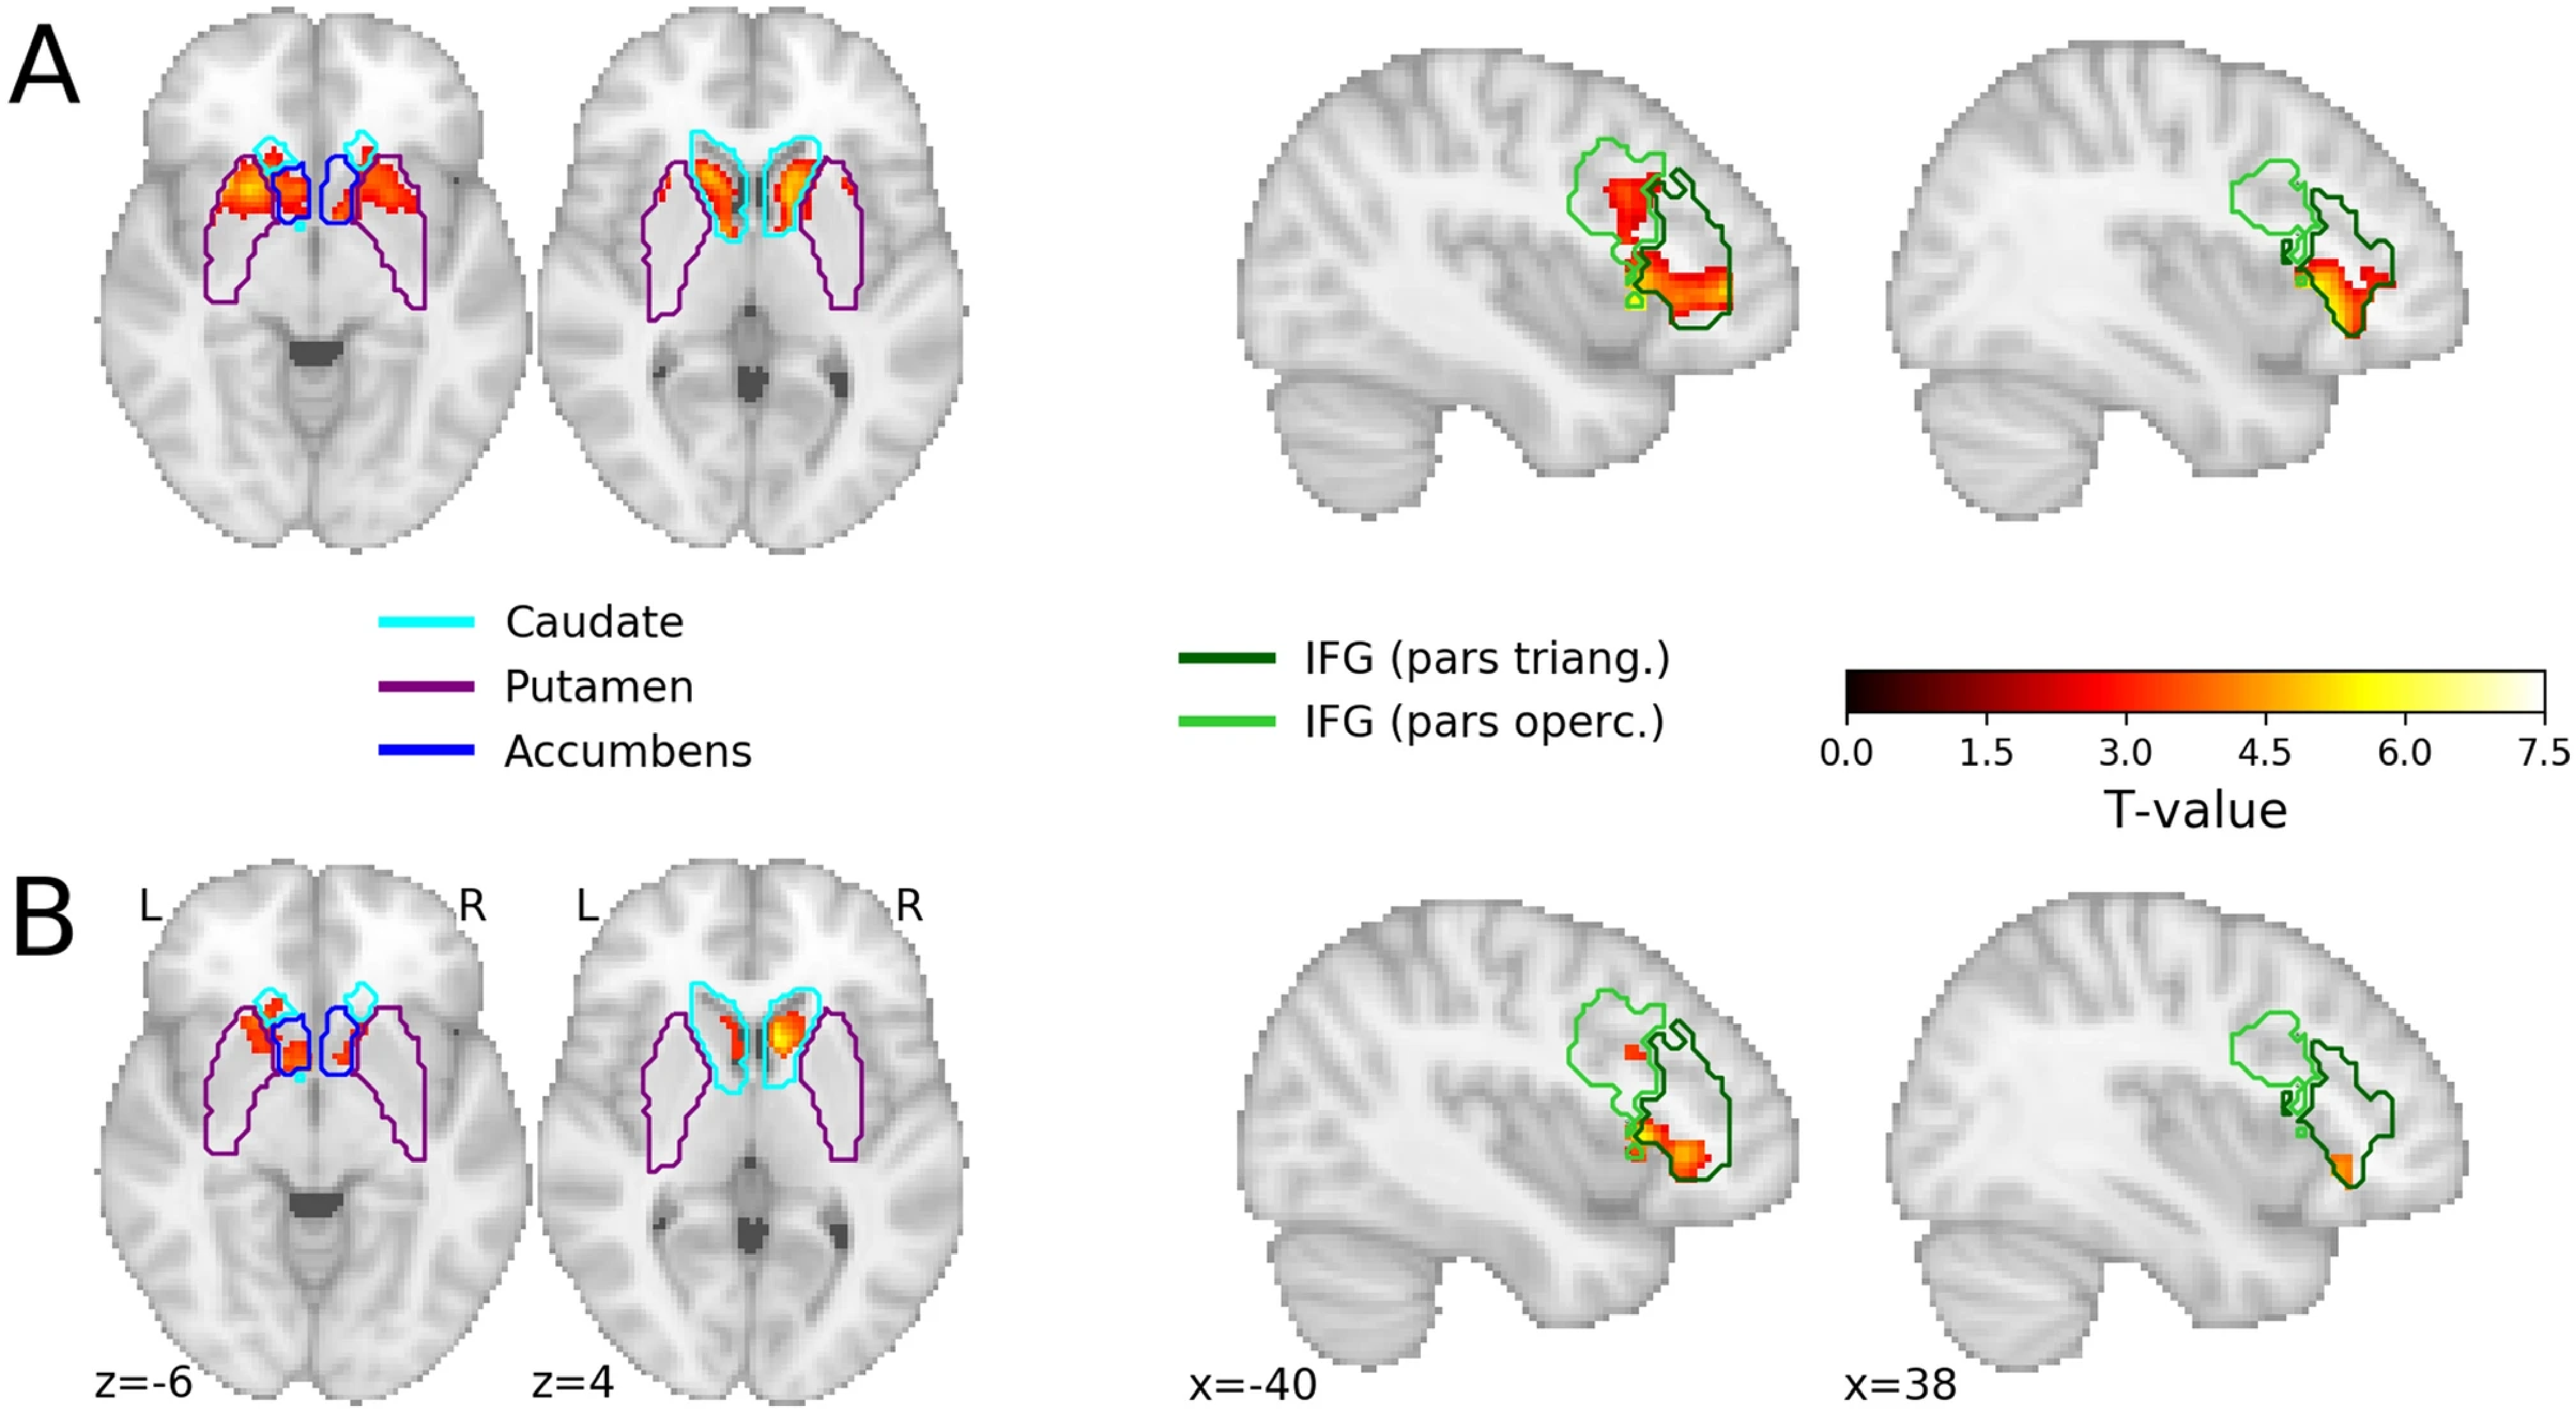
\includegraphics{_bookdown_files/morbid-curiosity-files/figures/figure_2.pdf}
\caption{\label{fig:fig-morbid-curiosity-2}Results of confirmatory ROI analyses for the induction phase (\textbf{A}) the contrast negative\textsubscript{active\textgreater passive} (\textbf{B}) the contrast negative\textsubscript{active\textgreater passive} \textgreater{} positive\textsubscript{active\textgreater passive}. Voxels in red/yellow represent significant \emph{t}-values (\emph{p} \textless{} 0.05, corrected for multiple comparisons using the maximum statistic approach). The colored outlines represent the different brain regions within the probabilistic ROIs for the striatum (left) and inferior frontal gyrus (IFG; right). The outlines represent the border of the ROIs thresholded at 0. When voxels within one ROI had a nonzero probability in more than one brain region (e.g., the caudate and nucleus accumbens), the voxel was assigned to the brain region with the largest probability.}
\end{figure}



Our second set of hypotheses focused on comparing a choice for negative information with a choice for positive information, controlling for general semantic, affective and visual processing (i.e., negative\textsubscript{active\textgreater passive} \textgreater{} positive\textsubscript{active\textgreater passive}). As predicted, a confirmatory ROI analysis demonstrated more activation in the striatum when participants viewed a negative cue that was chosen as compared to a positive cue that was chosen, relative to watching that same negative or positive cue in the passive-viewing condition. Again, significant voxels were found across the striatum, in the caudate, putamen and NAcc. A similar effect was found in the IFG (see Figure \ref{fig:fig-morbid-curiosity-2}). To explore the directionality of the effects, we extracted the parameter weights (\(\hat{\beta}\)) for the individual regressors for both ROIs. A visual inspection of plotted weights suggest that the patterns of neural activation reported for the striatum, are driven both by activation in the striatum when viewing negative cues in the active-choice condition, and deactivation in the striatum when viewing negative cues in the passive-viewing condition. Further details can be found in Figure \ref{fig:fig-morbid-curiosity-S1} of the \protect\hyperlink{morbid-curiosity-supplement}{Supplementary Materials}.

\hypertarget{whole-brain-analyses}{%
\subsection{Whole-brain analyses}\label{whole-brain-analyses}}

In addition to the confirmatory analyses reported above, we performed a whole-brain analysis (cluster-corrected with a voxel-wise threshold of \emph{p} \textless{} 0.005 and a cluster-wise threshold of \emph{p} \textless{} 0.05) for the two confirmatory contrasts (see Figure \ref{fig:fig-morbid-curiosity-3}). In addition to activation in the regions targeted in the confirmatory ROI analyses, the whole-brain analyses for the negative\textsubscript{active\textgreater passive} contrast demonstrated robust activation in the ACC, paracingulate gyrus, superior frontal gyrus, middle frontal gyrus, OFC, insular cortex, frontal operculum, frontal pole, temporal pole, thalamus and brain stem, when participants viewed a negative cue that was chosen (in the active-choice condition) as compared to watching that same negative cue in the passive-viewing condition. A complete table of the significant clusters can be found in the \protect\hyperlink{morbid-curiosity-supplement}{Supplementary Materials} (Table \ref{tab:tab-morbid-curiosity-S2}, as well as the significant clusters associated with the positive\textsubscript{active\textgreater passive} contrast, Table \ref{tab:tab-morbid-curiosity-S3}). The whole-brain results for the negative\textsubscript{active\textgreater passive} \textgreater{} positive\textsubscript{active\textgreater passive} contrast are presented in Table \ref{tab:tab-morbid-curiosity-1}. This contrast demonstrated stronger activation in the ACC, paracingulate gyrus, superior frontal gyrus, OFC, insular cortex and frontal operculum, when participants viewed a negative cue that was chosen as compared to a positive cue that was chosen (relative to watching that same negative or positive cue in the passive-viewing condition).

\begin{figure}
\centering
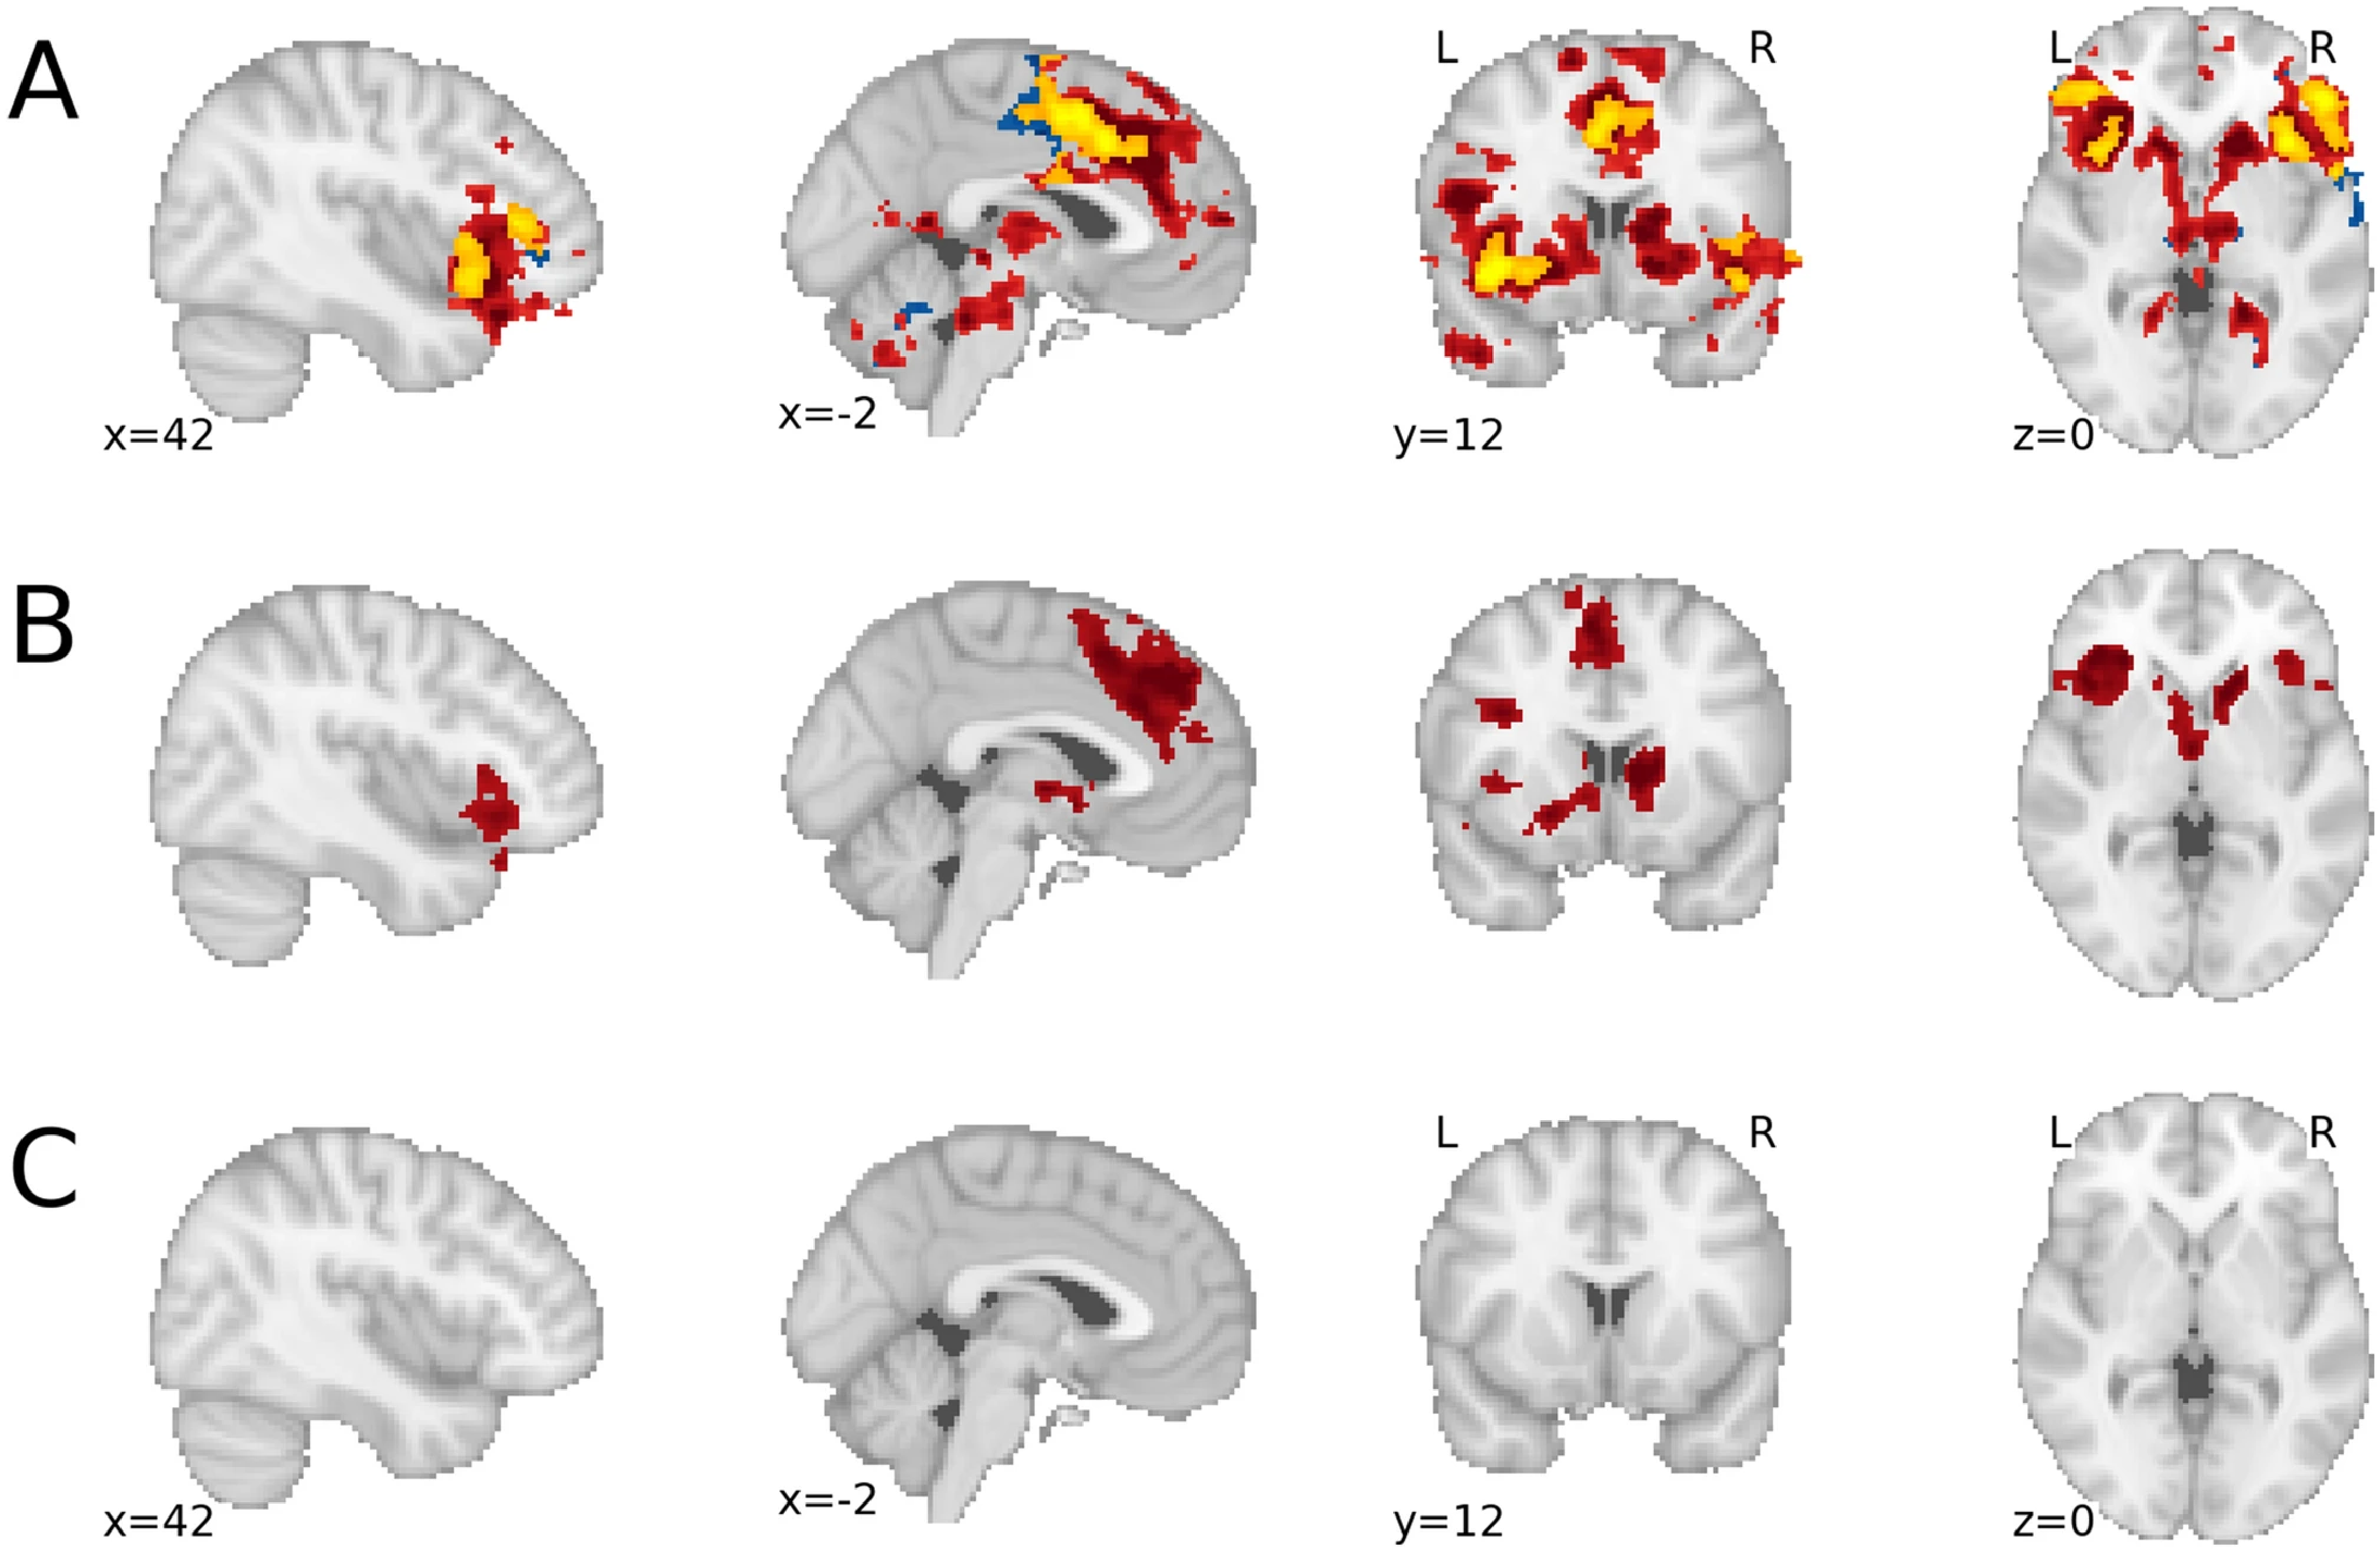
\includegraphics{_bookdown_files/morbid-curiosity-files/figures/figure_3.pdf}
\caption{\label{fig:fig-morbid-curiosity-3}Results of the exploratory whole-brain analyses for the induction phase: (\textbf{A}) the contrast negative\textsubscript{active\textgreater passive} (red), positive\textsubscript{active\textgreater passive} (blue), and their conjunction (yellow); (\textbf{B}) the contrast negative\textsubscript{active\textgreater passive} \textgreater{} positive\textsubscript{active\textgreater passive}; (\textbf{C}) the contrast positive\textsubscript{active\textgreater passive} \textgreater{} negative\textsubscript{active\textgreater passive} (empty).}
\end{figure}



\begingroup\fontsize{9}{11}\selectfont

\begin{ThreePartTable}
\begin{TableNotes}[para]
\item \textit{Note: } 
\item The X, Y, and Z coordinates refer to MNI152 (2 mm) space. The regions are taken from the Harvard–Oxford (sub)cortical atlas and voxels are assigned to regions based on their maximum probability across all ROIs within the atlas. *K* refers to the number of voxels within a particular region.
\end{TableNotes}
\begin{longtabu} to \linewidth {>{\raggedleft\arraybackslash}p{1em}>{\raggedleft\arraybackslash}p{1em}>{\raggedleft\arraybackslash}p{1em}>{\raggedright\arraybackslash}p{1em}>{\raggedleft\arraybackslash}p{1em}>{\raggedleft\arraybackslash}p{1em}>{\raggedright}X>{\raggedleft\arraybackslash}p{1em}>{\raggedleft\arraybackslash}p{1em}}
\caption{\label{tab:tab-morbid-curiosity-1}Cluster statistics and associated brain regions from the exploratory whole-brain analysis.}\\
\toprule
Cluster nr & Cluster size & Cluster max & X & Y & Z & Region & K & Max\\
\midrule
1 & 3158 & 4.82 & − 8 & 30 & 24 & Left paracingulate gyrus & 831 & 4.58\\
 &  &  &  &  &  & Right paracingulate gyrus & 741 & 4.70\\
 &  &  &  &  &  & Left superior frontal gyrus & 657 & 4.64\\
 &  &  &  &  &  & Right cingulate gyrus, anterior division & 317 & 4.42\\
 &  &  &  &  &  & Left cingulate gyrus, anterior division & 300 & 4.82\\
\addlinespace
 &  &  &  &  &  & Right superior frontal gyrus & 201 & 3.94\\
 &  &  &  &  &  & Left juxtapositional lobule cortex & 76 & 3.27\\
 &  &  &  &  &  &  &  \vphantom{3} & \\
2 & 1928 & 4.84 & − 42 & 20 & 4 & Left frontal orbital cortex & 602 & 4.64\\
 &  &  &  &  &  & Left insular cortex & 234 & 4.17\\
\addlinespace
 &  &  &  &  &  & Left inferior frontal gyrus, pars triangularis & 229 & 4.17\\
 &  &  &  &  &  & Left frontal operculum cortex & 205 & 4.84\\
 &  &  &  &  &  & Left inferior frontal gyrus, pars opercularis & 93 & 3.65\\
 &  &  &  &  &  & Left temporal pole & 57 & 4.31\\
 &  &  &  &  &  & Left subcallosal cortex & 29 & 3.22\\
\addlinespace
 &  &  &  &  &  & Left caudate & 121 & 3.48\\
 &  &  &  &  &  & Left Putamen & 110 & 3.86\\
 &  &  &  &  &  & Left thalamus & 48 & 3.84\\
 &  &  &  &  &  & Left accumbens & 39 & 3.52\\
 &  &  &  &  &  &  &  \vphantom{2} & \\
\addlinespace
3 & 692 & 4.64 & 36 & 24 & -16 & Right frontal orbital cortex & 443 & 4.64\\
 &  &  &  &  &  & Right insular cortex & 79 & 3.80\\
 &  &  &  &  &  & Right frontal operculum cortex & 70 & 3.39\\
 &  &  &  &  &  & Right temporal pole & 44 & 3.40\\
 &  &  &  &  &  & Right inferior frontal gyrus, pars triangularis & 30 & 3.27\\
\addlinespace
 &  &  &  &  &  &  &  \vphantom{1} & \\
4 & 464 & 4.74 & 10 & 14 & 4 & Right caudate & 265 & 4.74\\
 &  &  &  &  &  & Right putamen & 26 & 3.49\\
 &  &  &  &  &  &  &  & \\
5 & 296 & 3.81 & − 36 & 12 & 26 & Left middle frontal gyrus & 111 & 3.72\\
\addlinespace
 &  &  &  &  &  & Left inferior frontal gyrus, pars opercularis & 111 & 3.81\\
 &  &  &  &  &  & Left precentral gyrus & 64 & 3.46\\
\bottomrule
\insertTableNotes
\end{longtabu}
\end{ThreePartTable}
\endgroup{}

To further interpret the whole brain results, we used the ``decoder'' function from Neurosynth (Yarkoni et al., \protect\hyperlink{ref-yarkoni2011large}{2011}) to find key terms associated with particular patterns of neural activation. The neural pattern produced by the negative\textsubscript{active\textgreater passive} \textgreater{} positive\textsubscript{active\textgreater passive} contrast resulted in the following key terms (top-10): reward, task, monetary, semantic, anticipation, incentive, demands, fear, autobiographical, retrieval (see \protect\hyperlink{morbid-curiosity-supplement}{Supplementary Materials}, Table \ref{tab:tab-morbid-curiosity-S1}). Although it is important to be careful with drawing reverse inference conclusions about the psychological meaning of neural activation (Poldrack, \protect\hyperlink{ref-poldrack2006can}{2006}), these terms at minimum suggest that the neural pattern associated with choosing negative content (relative to choosing positive content and passive-viewing) is similar to neural patterns associated with reward and the processing of extrinsic incentives.

It is important to note that none of the confirmatory ROI analyses nor any of our exploratory analyses showed significant differences in the relief phase (i.e., when viewing the image). This is in line with previous work on curiosity (Gruber et al., \protect\hyperlink{ref-gruber2014states}{2014}) that found robust neural activation when inducing curiosity (e.g., presentation of trivia questions), but not when relieving curiosity (e.g., presentation of trivia answers). Other work on curiosity, that did find differences in the relief phase, contrasted a condition in which curiosity was relieved, with a condition that withheld information (Lieshout et al., \protect\hyperlink{ref-van2018induction}{2018}) or a condition that showed irrelevant information (Jepma et al., \protect\hyperlink{ref-jepma2012neural}{2012}). In the present study, however, we contrasted the relief phase in the active-choice condition with viewing the exact same information in the passive-viewing condition. Since we found that participants in the passive-viewing condition also reported a reasonable amount of curiosity in response to the cue, curiosity relief may have occurred in both the active-choice and the passive-viewing condition.

\hypertarget{morbid-curiosity-discussion}{%
\section{Discussion}\label{morbid-curiosity-discussion}}

In the last decade, neuroscientific research has made a major contribution to a better understanding of choice, value and curiosity. Most of this work, however, has focused on extrinsically rewarding information (Bartra et al., \protect\hyperlink{ref-bartra2013valuation}{2013}; Braver et al., \protect\hyperlink{ref-braver2014mechanisms}{2014}), or on an intrinsically-motivated curiosity for neutral or positive information (e.g., Gruber \& Ranganath, \protect\hyperlink{ref-gruber2019curiosity}{2019}; Kang et al., \protect\hyperlink{ref-kang2009wick}{2009}; Lieshout et al., \protect\hyperlink{ref-van2018induction}{2018}). The present study demonstrates that choosing intensely \emph{negative} stimuli engages similar brain regions as those that support extrinsic incentives and regular curiosity (Bartra et al., \protect\hyperlink{ref-bartra2013valuation}{2013}; Diekhof et al., \protect\hyperlink{ref-diekhof2012role}{2012}; Gruber \& Ranganath, \protect\hyperlink{ref-gruber2019curiosity}{2019}; Kidd \& Hayden, \protect\hyperlink{ref-kidd2015psychology}{2015}; Sakaki et al., \protect\hyperlink{ref-sakaki2018curiosity}{2018}). We found that a deliberate choice for death, violence or harm is associated with activation in the striatum (NAcc, caudate and putamen), inferior frontal gyrus, anterior insula, orbitofrontal cortex and anterior cingulate cortex. This pattern was present both when we contrasted negative cues (that were chosen) with passively viewing these cues, and when we contrasted negative cues (that were chosen) with positive cues (that were chosen), controlling for passive viewing. These findings reflect the induction phase in which participants anticipated on their choice; we found no differences in the relief phase in which participants viewed images.

Although we found activation in regions associated with reward and incentives, it is important to be careful with the conclusion that it is ``rewarding'' to choose negative information (Poldrack, \protect\hyperlink{ref-poldrack2006can}{2006}). Reward regions are associated with a multitude of psychological processes (Bartra et al., \protect\hyperlink{ref-bartra2013valuation}{2013}), and reward is a construct with different dissociable dimensions, including ``liking'' and ``wanting'' (e.g., Berridge et al., \protect\hyperlink{ref-berridge2009dissecting}{2009}; Weber et al., \protect\hyperlink{ref-weber2018frontostriatal}{2018}). In addition, the distributed pattern of activation that we found most likely reflects psychological processes beyond reward as well. In the next section, we address several, non-mutually exclusive, interpretations of this distributed pattern, including an interpretation regarding the potential reward value of negativity, the possibility that this neural pattern reflects uncertainty, and an interpretation that considers the particular characteristics of the task.

Golman \& Loewenstein (\protect\hyperlink{ref-golman2015curiosity}{2015}) propose that a desire to obtain information can be driven by a motive to make better decisions, a motive to experience pleasantness, or a motive to engage with information ``for its own sake'' (p.~3). The negative choices made by our participants are most likely consistent with the latter intrinsic motive. Participants chose images that were not hedonically pleasing and, in contrast to other recent (neuroscientific) studies targeting curiosity (e.g., Lieshout et al., \protect\hyperlink{ref-van2018induction}{2018}; Kobayashi et al., \protect\hyperlink{ref-kobayashi2019diverse}{2019}), there was no monetary outcome associated with choosing (negative) images. The question that follows then is: what is the value of negativity?

One possibility is that knowledge acquisition is inherently valuable (Marvin \& Shohamy, \protect\hyperlink{ref-marvin2016curiosity}{2016}; Murayama et al., \protect\hyperlink{ref-murayama2019process}{2019}), even when people acquire knowledge about negative social situations that involve death, violence or harm. Indeed, the knowledge update that follows from engaging with negative information might be valuable for building a realistic model of the world (Baumeister et al., \protect\hyperlink{ref-baumeister2001bad}{2001}) or for dealing with future aversive situations. Applying this interpretation to our findings, we propose that the brain predicts a larger information gain in the negative choice condition than in the positive choice condition. This is reflected in stronger activation of reward circuitry (e.g., NAcc, caudate, putamen) that might track the expected value of knowledge acquisition (Murayama et al., \protect\hyperlink{ref-murayama2019process}{2019}), or the salience of the information (Bartra et al., \protect\hyperlink{ref-bartra2013valuation}{2013}). Note that we focus here on the informational value of valenced stimuli in epistemic terms (Berlyne, \protect\hyperlink{ref-berlyne1966curiosity}{1966}; Litman, \protect\hyperlink{ref-litman2005curiosity}{2005}; Loewenstein, \protect\hyperlink{ref-loewenstein1994psychology}{1994}; Murayama et al., \protect\hyperlink{ref-murayama2019process}{2019}), but the value of choosing to engage with negative or positive stimuli may also lie in the emotional experiences or sensations that are evoked by the stimulus (Zuckerman, \protect\hyperlink{ref-zuckerman1979}{1979}; Zuckerman \& Litle, \protect\hyperlink{ref-zuckerman1986personality}{1986}; see for an overview Tamir, \protect\hyperlink{ref-tamir2016people}{2016}).

Another possible explanation for the present findings lies in the momentary uncertainty that people may experience when viewing negative cues (e.g., How extreme will the image be?), in combination with the predicted reduction of this uncertainty when choosing to view images. Curiosity is often seen as a desire to resolve uncertainty (Berlyne, \protect\hyperlink{ref-berlyne1966curiosity}{1966}; Gottlieb \& Oudeyer, \protect\hyperlink{ref-gottlieb2018towards}{2018}; Loewenstein, \protect\hyperlink{ref-loewenstein1994psychology}{1994}) and several recent studies have demonstrated that people experience higher levels of curiosity for uncertain stimuli (Kobayashi et al., \protect\hyperlink{ref-kobayashi2019diverse}{2019}; Lieshout et al., \protect\hyperlink{ref-van2018induction}{2018}). People even engage with aversive stimuli to reduce uncertainty, preferring a reduction in uncertainty above a negative outcome (Hsee \& Ruan, \protect\hyperlink{ref-hsee2016pandora}{2016}). Neuroscience studies have shown that uncertainty is associated with activation in the OFC, ACC and anterior insula (Bach \& Dolan, \protect\hyperlink{ref-bach2012knowing}{2012}; Harris et al., \protect\hyperlink{ref-harris2008functional}{2008}; Singer et al., \protect\hyperlink{ref-singer2009common}{2009}), regions we also found to be active in the active-choice condition. Moreover, we found that the OFC, ACC and anterior insula were more strongly engaged when viewing chosen negative cues, as compared to chosen positive cues. The neural pattern found in the negative choice condition (as compared to the positive choice condition) may thus reflect a higher level of outcome uncertainty, and/or a stronger expected reduction in uncertainty, in interaction with, or irrespective of (Harris et al., \protect\hyperlink{ref-harris2008functional}{2008}), the reward value of the information.

A final interpretation of the present findings revolves around the demands of the task that people performed in the choice-condition. Deciding how to respond to a negative cue may be an engaging and effortful task, that requires careful weighing of options. Several perspectives suggests that the IFG and ACC may support such processes. In a recent framework, Gruber et al. (\protect\hyperlink{ref-gruber2014states}{2014}) propose that curiosity involves an appraisal process, supported by the IFG, that determines one's ability to deal with information (see also Silvia, \protect\hyperlink{ref-silvia2008interest}{2008}). Notably, they predict enhanced involvement of the IFG in situations that involve a dilemma in which people have to choose between approaching or avoiding information. Other authors have suggested that the dACC may be particularly active in effortful or exploratory tasks that demand cognitive control, as compared to tasks that can be performed by engaging in automatic behavior (Shenhav et al., \protect\hyperlink{ref-shenhav2016dorsal}{2016}). When applying these perspectives to the current findings, stronger ACC and/or IFG activation for negative choice as opposed to passive viewing may reflect the specific cognitive demands (e.g., appraisal, weighing options, effort) of the active-choice condition relative to the passive-viewing condition. Furthermore, stronger ACC and/or IFG activation for negative choice as opposed to positive choice may reflect the relatively complex cost--benefit analysis that precedes a choice to choose a negative stimulus, as compared to the relatively automatic or ``default'' decision to choose a positive stimulus. This interpretation is consistent with the characterization of ``morbid curiosity'' as a conflict state, in which people ``want'' information that they do not ``like'' (Litman, \protect\hyperlink{ref-litman2005curiosity}{2005}; Rimé et al., \protect\hyperlink{ref-rime2005brief}{2005}).

The present study has a few limitations that we should address. First of all, all contrasts calculated in the present study are relative to the passive-viewing condition (as preregistered). We deliberately made this decision, because we wanted to isolate the neural activation associated with a deliberate choice to view a stimulus. More specifically, in a direct contrast between chosen negative cues and chosen positive cues, it would have been impossible to know whether the pattern of neural activation was driven by \emph{choosing} negative versus positive information, or by simply \emph{viewing} negative versus positive cues. The yoked procedure, and the resulting contrasts, control for the latter, since activation associated with viewing negative versus positive cues is subtracted out. Furthermore, confronting participants with emotional material that they cannot control, is common practice when scientists study affective/emotional experience (Lang \& Bradley, \protect\hyperlink{ref-lang2010emotion}{2010}; Lindquist et al., \protect\hyperlink{ref-lindquist2016brain}{2016}) and emotion regulation (Buhle et al., \protect\hyperlink{ref-buhle2014cognitive}{2014}; Wager et al., \protect\hyperlink{ref-wager2008prefrontal}{2008}), and thus serves as a meaningful control condition. Nevertheless, it is important to note that our results in the striatum were partly driven by deactivation in the passive viewing condition (see Figure \ref{fig:fig-morbid-curiosity-S1}, \protect\hyperlink{morbid-curiosity-supplement}{Supplementary Materials}). Since this pattern of deactivation was not predicted in our preregistered analysis protocol, and our study was not designed for optimal detection of directional effects, we will not discuss this finding further. A design that contrasts choosing versus passive viewing within-subjects may clarify whether explicitly anticipating a negative outcome that cannot be controlled indeed deactivates the striatum.

Second, the present design does not allow for a contrast between agreeing to view an image and refusing to view an image, because participants said ``yes'' to the cue in the vast majority of the trials (i.e., 81\% for negative cues; 95\% for positive cues). As a future direction, it may be insightful to develop a design that artificially balances yes and no responses within the same participant to investigate differences in reward circuitry between approaching and avoiding negative information. In the present study, however, we deliberately chose not to restrict or disregard participant's choices, because we wanted to keep the decision process as natural as possible. Having said that, a fMRI scanner is a relatively boring environment, and previous research has shown that boredom prompts people to seek out novel experiences (Bench \& Lench, \protect\hyperlink{ref-bench2019boredom}{2019}). Thus, the scanning environment may have stimulated participants to say yes more often (across both conditions) than they would have done in other settings.

A third limitation is that we cannot rule out the possibility that arousal contributes to our findings when contrasting negative and positive cues. Although we matched the social negative and positive cues (and images) in terms of valence extremity (i.e., positive cues were perceived as equally positive as negative cues were perceived as negative), the cues (and images) were not matched in terms of arousal. We accepted the difference in arousal as a consequence of the content criterion for negative images (i.e., displaying death, violence or harm within a social context), and our deliberate choice not to include erotic images, considering the practical considerations associated with erotic content (Wierzba et al., \protect\hyperlink{ref-wierzba2015erotic}{2015}). It is important to note that in the negative choice vs.~passive-viewing contrast the effect of viewing an arousing cue is subtracted out. The negative choice vs.~positive choice contrast, however, does not control for the net difference between the arousing quality of the negative and positive cues. Therefore, it is possible that the pattern of neural activation when comparing negative vs.~positive choice, in particular in the ACC and insula (Citron et al., \protect\hyperlink{ref-citron2014emotional}{2014}; Satpute et al., \protect\hyperlink{ref-satpute2019deconstructing}{2019}), reflects, to some extent, the higher arousal value of the negative vs.~positive verbal cues.

A fourth and final limitation is that the present study focused on behavior, without incorporating trial-by-trial ratings of curiosity. This restricts the extent to which the present findings speak to the subjective experience of curiosity. In regular curiosity, for example when processing trivia questions, there are little costs associated with acting on curiosity, and thus it may be sufficient to focus on subjective ratings of curiosity. With morbid curiosity, however, the stakes are higher. Although people can experience curiosity for a negative stimulus without choosing to engage with it, behavior is, in our opinion, the most straightforward indicator of how the conflict state of morbid curiosity is resolved. In other words, only when people choose to engage with negative information can we deduce that the predicted benefits (e.g., knowledge acquisition, uncertainty reduction) outweigh the predicted costs of engaging with the information (e.g., not being able to cope with the content). Furthermore, a focus on choice connects to the many behavioral expressions of this phenomenon in the real world (e.g., ``rubbernecking'' on the freeway; clicking on a social media link). Future research should investigate whether the subjective experience of curiosity for negative stimuli is associated with a similar neural pattern (e.g., reward circuitry, ACC, insula, OFC) as the pattern found with the present choice paradigm.

Despite the questions that the present study provokes, our findings represent an important step in nuancing models of decision-making, valuation and curiosity. In light of the ubiquity of exploring negativity in daily life, we believe that it is crucial to start thinking about the value of seeking out negative content.

\hypertarget{hypothesis-kernel-analysis}{%
\chapter{Explainable models of facial movements predict emotion perception behavior}\label{hypothesis-kernel-analysis}}

\chaptermark{Explainable models of facial movements}

\newpage
\normalsize

\begin{abstract}
Since Darwin, many studies have proposed how action units (AUs) relate to categorical emotions, giving rise to a multitude of hypothesized AU-emotion mappings. The qualitative nature of these mappings prevent us from quantifying to what extent these AU-based mappings explain categorical emotions. Here, we formalize these qualitative mappings as quantitative, predictive models that are able to precisely quantify the importance and limitations of AUs for emotion perception. We use a state-of-the-art modelling approach to compare these models in their capacity to \emph{predict} human emotion classification behavior, \emph{explain} the role of each AU, and \emph{explore} how models can be improved. Additionally, by estimating the noise ceiling of predictive models, we estimate the limitations of these AU-based models due to individual differences. Together, our approach enables rigorous testing of different models, which quantifies the importance and limitations of AU-based models and proposes how to proceed in building better models of emotion perception.
\end{abstract} \newpage

\hypertarget{hka-introduction}{%
\section{Introduction}\label{hka-introduction}}

Facial expressions are a powerful and efficient medium to express and transmit a wide variety of emotions (Jack \& Schyns, \protect\hyperlink{ref-Jack2015-sh}{2015}). Since the pioneering work of Ekman and Friesen (Ekman \& Friesen, \protect\hyperlink{ref-Ekman1976-hm}{1976}; Friesen \& Ekman, \protect\hyperlink{ref-Friesen1978-tp}{1978}), studies have attempted to describe and quantify the relationship between facial expressions and emotions. Central to this endeavor are ``action units'' (AUs) --- the smallest visually discriminable movements of the face (J. F. Cohn et al., \protect\hyperlink{ref-Cohn2007-az}{2007}). Many studies have proposed that specific combinations of AUs represent different categorical emotions (Barrett et al., \protect\hyperlink{ref-Barrett2019-bc}{2019}; Matsumoto et al., \protect\hyperlink{ref-Matsumoto2008-qk}{2008}). For example, Friesen \& Ekman (\protect\hyperlink{ref-Friesen1978-tp}{1978}) proposed that the facial expression of anger comprises Brow Lowerer (AU4), Upper Lid Raiser (AU5), Lid Tightener (AU7), and Lip Tightener (AU23). Such mappings between combinations of AUs and emotions are supposedly largely invariant to individual differences (Ekman \& Keltner, \protect\hyperlink{ref-Ekman1997-bk}{1997}; Izard, \protect\hyperlink{ref-Izard1994-ca}{1994}; Matsumoto et al., \protect\hyperlink{ref-Matsumoto2008-qk}{2008}), implying that facial expressions conforming to the hypothesized AU combination will be consistently interpreted as the associated emotion. However, the importance of AUs in emotion perception and the invariance of the AU-emotion mappings is still debated (Barrett et al., \protect\hyperlink{ref-Barrett2019-bc}{2019}; Jack et al., \protect\hyperlink{ref-Jack2012-eq}{2012}, \protect\hyperlink{ref-Jack2009-yy}{2009}).

\hypertarget{the-prediction-explanation-exploration-framework}{%
\subsection{The prediction-explanation-exploration framework}\label{the-prediction-explanation-exploration-framework}}

To compare different combinations of AUs in relation to categorical perception of emotions, one would need to directly and quantitatively compare the mappings hypothesized in different theories. In mature scientific endeavors, evaluating and comparing hypotheses is done using formal models, which can be quantitatively assessed by how accurately they are able to \emph{predict} phenomena. In addition, models are used to \emph{explain} the underlying causes of phenomena, and, with the enhanced understanding these explanations can provide, allow us to \emph{explore} new predictions about the phenomenon (see Figure \ref{fig:fig-hka-1}). Most AU-emotion mappings, however, are not based or estimated from an explicit model, but are based on statistical tests between single AUs and discrete emotions (Cordaro et al., \protect\hyperlink{ref-Cordaro2018-xm}{2018}; Ekman et al., \protect\hyperlink{ref-Ekman1980-of}{1980}; Jack et al., \protect\hyperlink{ref-Jack2012-eq}{2012}; Wiggers, \protect\hyperlink{ref-Wiggers1982-na}{1982}). The result describes a hypothesized relationship between a combination of AUs and a categorical emotion, which requires further developments to become formally predictive. We address this development with a novel methodology that formalizes descriptive hypotheses, such as AU-emotion mappings, as predictive models of classification (see \protect\hyperlink{hka-methods}{Methods}). To evaluate these formal models, we quantify how well they \emph{predict} the representation of emotions (via their behavioral classification performance), \emph{explain} how different AUs contribute to these causal representations, and \emph{explore} how we can improve existing models using insights from the derived explanations.

This \emph{prediction-explanation-exploration} framework (see Figure \ref{fig:fig-hka-1}) is a rigorous methodology to estimate the proportion of variance in categorization behavior that \emph{can} be attributed to the AU models of the emotions vs.~\emph{cannot} be attributed the models themselves. We estimated the latter with the component of behavioral variance that arises from individual differences in the interpretation of the AU combinations --- i.e., the noise ceiling (Lage-Castellanos et al., \protect\hyperlink{ref-lage2019methods}{2019}; Nili et al., \protect\hyperlink{ref-Nili2014-ar}{2014}). The noise ceiling proposes that a fixed model cannot, by definition, explain any variations between individuals who categorize facial expressions with this model. Here, we use noise ceilings to demonstrate the limitations of fixed, AU-based models of categorical emotions.

\begin{figure}
\centering
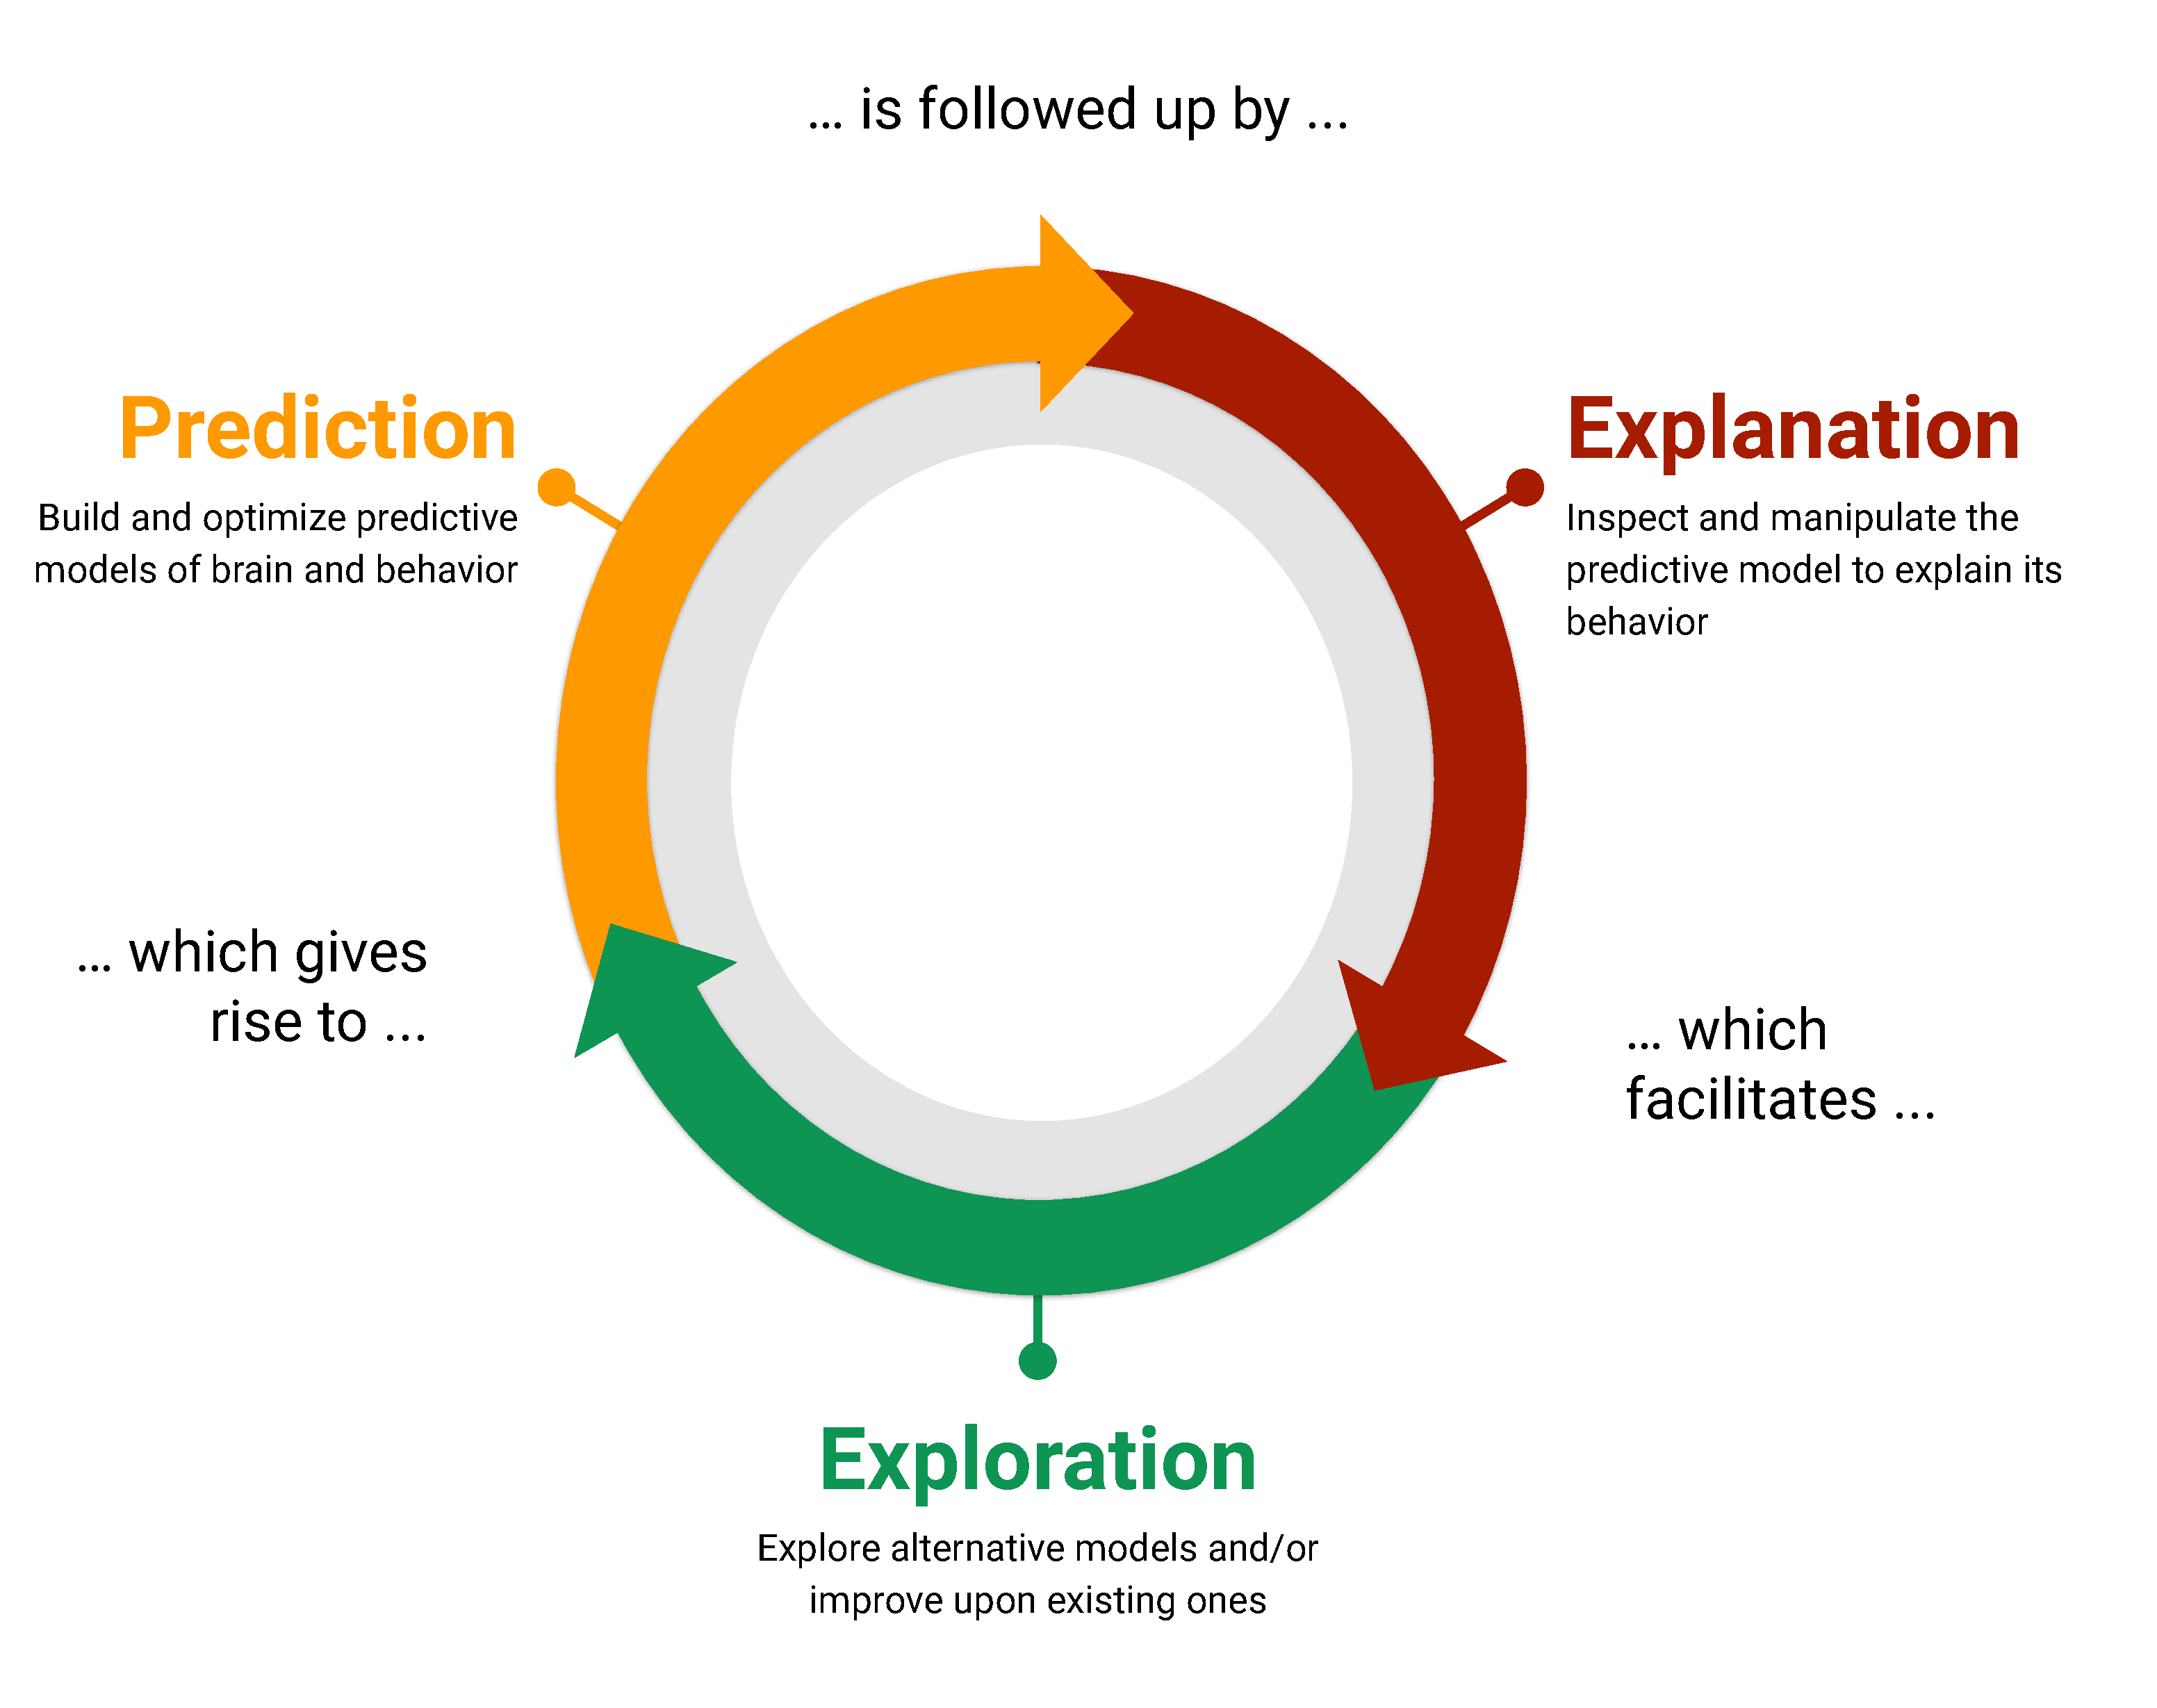
\includegraphics{_bookdown_files/hypothesis-kernel-analysis-files/figures/figure_1.pdf}
\caption{\label{fig:fig-hka-1}The modelling framework used in the current study, which uses models for prediction, explanation, and exploration.}
\end{figure}



We tested the ability of seven influential models of facial expressions of the six classic categorical emotions (see \protect\hyperlink{hka-methods}{Methods} and Table \ref{tab:tab-hka-1}) to predict categorical emotion labels. To do so, we used a psychophysics task containing a large set of dynamic facial expressions with random AU combinations. In this task, participants categorized each facial expression animation as one of the six classic emotions, or ``don't know.'' We used the models to \emph{predict}, for the same trials rated by the participants, the most likely emotion category, which were compared to the actual emotion ratings. Next, to \emph{explain} how specific AUs contributed to emotion classification performance, we systematically removed individual AUs from each model and recomputed its performance in predicting human behavior. Finally, we used these performance critical AUs to \emph{explore} whether they improved the predictions of models that do not represent them. We show that models of the AU-emotion relationship substantially improve their prediction performance when they comprise performance-critical AUs. However, because this performance remains below the noise ceiling, there is still model variance to explain, suggesting that the evaluated hypotheses AU-emotion relations tested are not optimal yet. Importantly, these noise ceilings indicate that individual differences contribute a large proportion of the variations in emotion categorizations, suggesting better models that include between-participant factors, such as culture and other perceiver-related characteristics.

\hypertarget{hka-methods}{%
\section{Methods}\label{hka-methods}}

\hypertarget{hypothesis-kernel-analysis-1}{%
\subsection{Hypothesis kernel analysis}\label{hypothesis-kernel-analysis-1}}

To formalize AU-emotion mappings as predictive models, we propose a novel method which we call ``hypothesis kernel analysis''. In the context of the current study, we use this method to reframe AU-emotion mappings as classification models that predict the probability of an emotion given a set of AUs (analogous to how people attempt to infer the emotion from others' facial emotion expressions; Jack \& Schyns, \protect\hyperlink{ref-Jack2015-sh}{2015}). In what follows, we conceptually explain how the method works. For a detailed and more mathematical description of the method, we refer the reader to the \protect\hyperlink{hypothesis-kernel-analysis-supplement}{Supplementary Methods}.

The underlying idea of the hypothesis kernel analysis is to predict a categorical dependent variable (e.g., the perceived emotion) based on the similarity between an \emph{observation} with a particular set of features (e.g., a face with a particular set of AUs; the independent variables) and statements of a \emph{hypothesis} (e.g., ``happiness is expressed by AUs 6 and 12''). This prediction can then be compared to real observations to evaluate the accuracy of the hypothesis. The three methodological challenges of this approach are how to measure the similarity between an observation and a hypothesis statement, how to derive a prediction based on this similarity, and how to compare the predictions to real data. Figure \ref{fig:fig-hka-2} outlines how we have solved these challenges in five steps, which we will describe in turn.

\begin{figure}
\centering
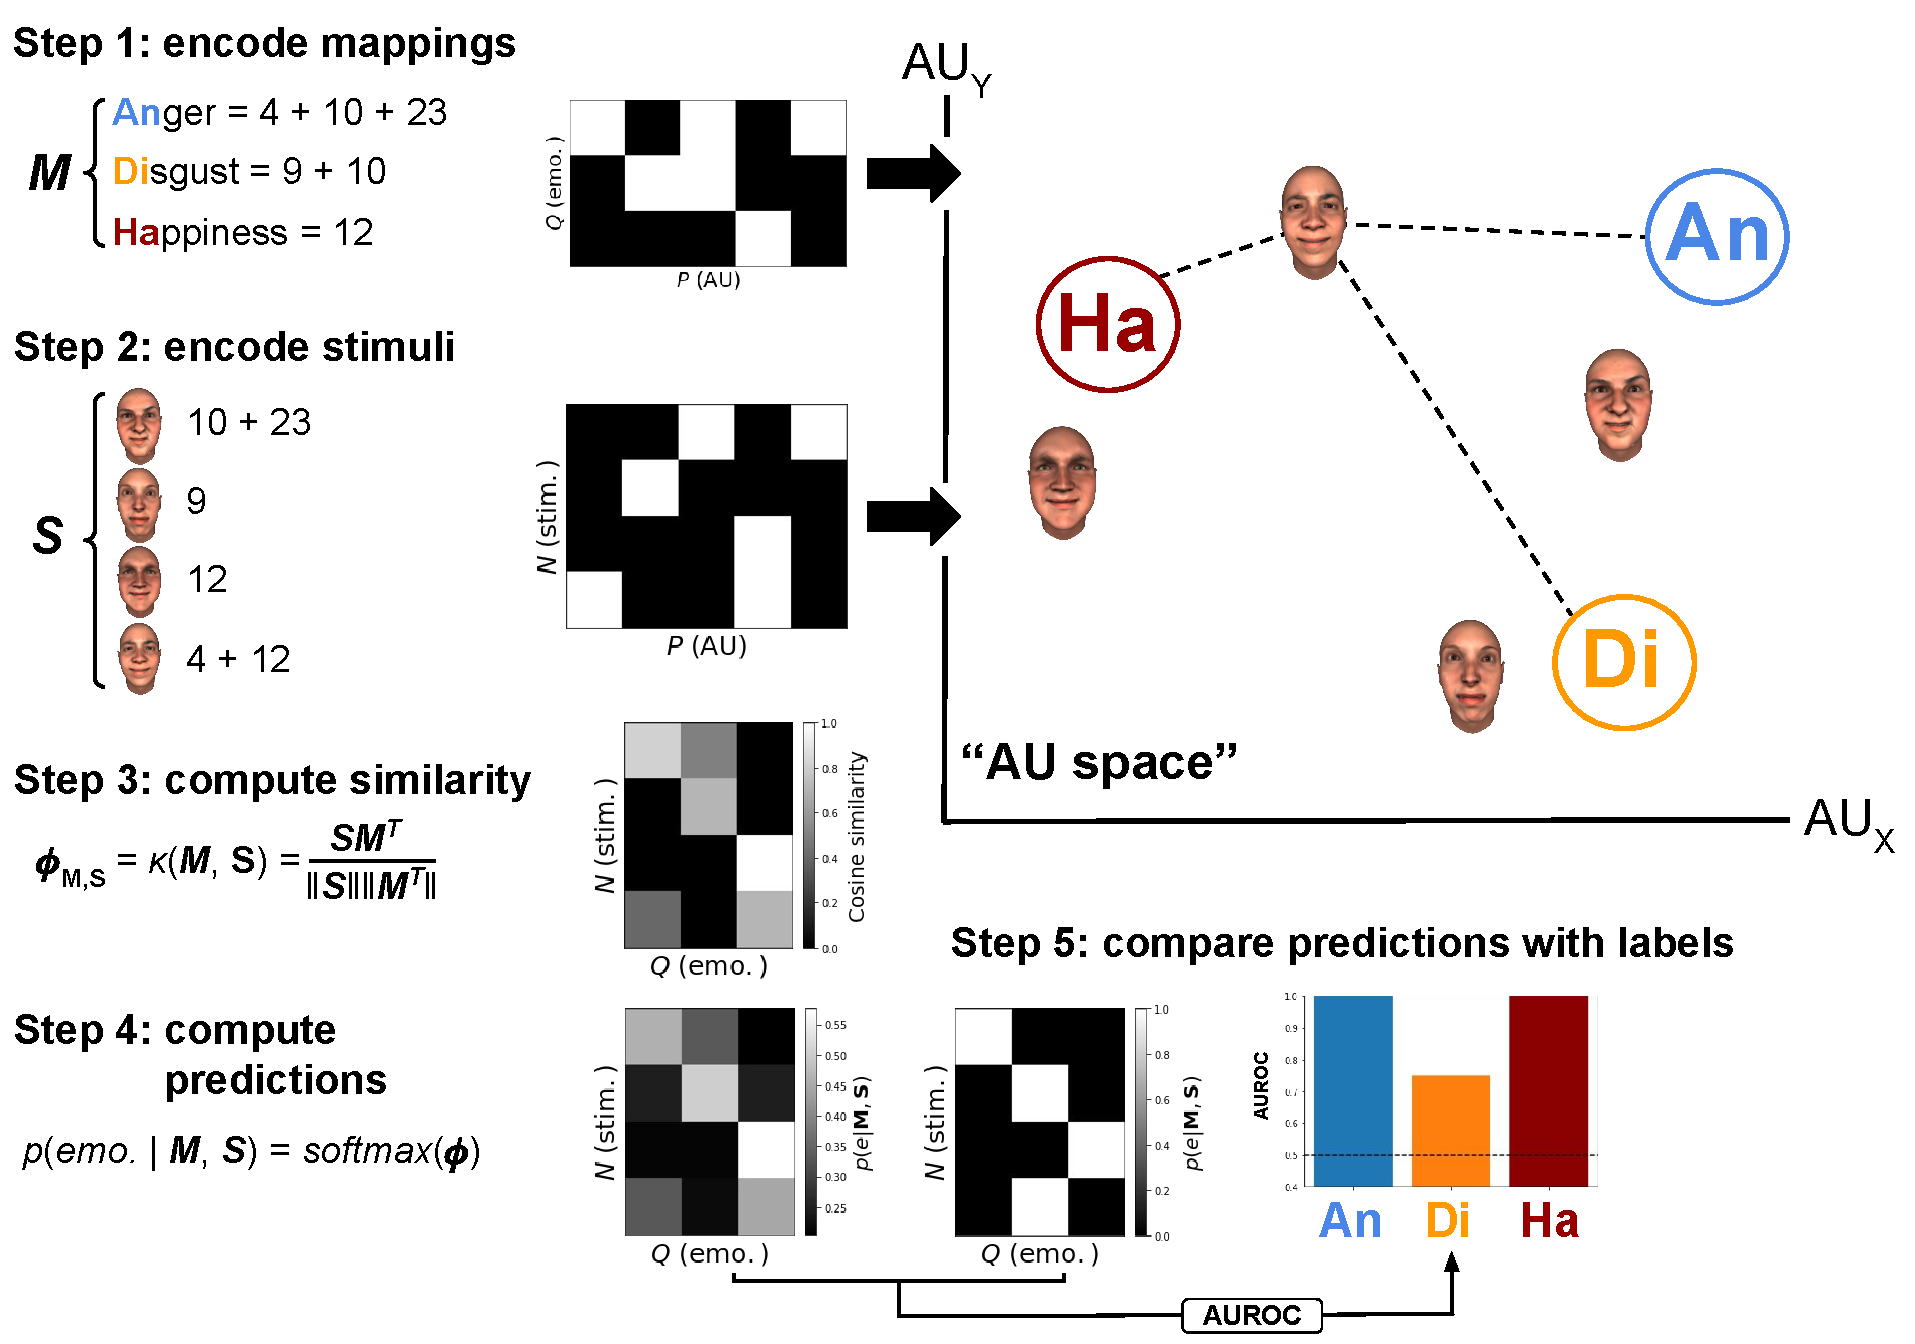
\includegraphics{_bookdown_files/hypothesis-kernel-analysis-files/figures/figure_2.pdf}
\caption{\label{fig:fig-hka-2}Schematic visualization of the proposed method using a set of hypothetical AU-emotion mappings (\(\mathbf{M}\)) and stimuli (\(\mathbf{S}\)) based on a small set of AUs (five in total). The variable \(P\) represents the number of variables (here: AUs), \(Q\) represents the number of classes (here: emotions), and \(N\) represents the number of trials (here: facial expression stimuli). Note that the AU space technically may contain any number of (\(P\)) dimensions, but is shown here in two dimensions for convenience.}
\end{figure}



To quantify the similarity between an observation and a hypothesis statement, we embed both in a multidimensional space that is spanned by a particular set of variables (e.g., different AUs). In this space, we start by representing each class of the dependent variable (corresponding to the statements of the hypothesis) as a separate point. In the current study, this amounts to embedding the different hypothesized AU configurations (e.g., ``happiness = AU12 + 6''; \(\mathbf{M}\) in Figure \ref{fig:fig-hka-2}) as points in ``AU space'', separately for each categorical emotion (see step 1 in Figure \ref{fig:fig-hka-2}). The coordinates of each point are determined by the hypothesized ``importance'' of each independent variable for that given class of the target variable. For example, the coordinates of each point in AU space represents the hypothesized relative intensity of each AU for a given emotion. As the AU-emotion mappings evaluated in the current study only specify whether an AU is included or excluded within a particular emotional configuration, we specify the coordinates of their embedding to be binary (0: excluded, 1: included). A different interpretation of the class embeddings described here is that they represent the location of a typical facial expression for this emotion in ``AU space'' according to a particular hypothesis.

As a second step, we embed each data point in the same space as the hypotheses. This means, the data used for this purpose should contain the same variables as were used to embed the hypotheses. For example, in this study, we use emotion ratings (i.e., the target variable) in response to dynamic facial expression stimuli with random configurations of AUs (i.e., the independent variables; \(\mathbf{S}\) in Figure \ref{fig:fig-hka-2}) to test the hypothesized AU-emotion mappings (see \protect\hyperlink{hka-dataset}{Dataset used to evaluate mappings}).

With the hypotheses and the data in the same space, the next step in our method is to compute, for each observation separately, the ``similarity'' between the data and each class of the target. For this purpose, we use \emph{kernel functions} (step 3 in Figure \ref{fig:fig-hka-2}), a technique that quantifies the similarity of two vectors. Any kernel function that computes a measure of similarity can be used, but in our analyses we use the cosine similarity as it normalizes the similarity by the magnitude (specifically, the L2 norm) of the data and hypothesis embeddings (but see Supplementary Figure \ref{fig:fig-hka-S3} for a comparison of model performance across different similarity and distance metrics).

As a fourth step, we interpret the similarity between the data and a given class embedding as being proportional to the evidence for a given class. In other words, the more similar a data point is to the statement of a hypothesis the stronger the prediction for the associated class. To produce a probabilistic prediction of the classes given a particular observation and hypothesis, we normalize the similarity values to the 0-1 range using the \emph{softmax} function (step 4 in Figure \ref{fig:fig-hka-2}).\footnote{Readers familiar with machine learning algorithms may recognize this as a specific implementation of a K-nearest neighbor classification model with \emph{K} = 1, which is fit on the embedded hypotheses (\(\mathbf{M}\)) and cross-validated on the data (\(\mathbf{S}\)).}

Finally, the accuracy of the model can be summarized by comparing its predictions to the actual values of the target variable in the dataset (see step 5 in Figure \ref{fig:fig-hka-2}). In this study, this means that the predictions are compared to the actual emotion ratings from participants. Although any model performance metric can be used, we use the ``Area under the Receiver operating curve'' (AUROC) as our model performance metric, because it is insensitive to class imbalance, allows for class-specific scores, and can handle probabilistic predictions (Dinga et al., \protect\hyperlink{ref-Dinga2020-si}{2020}). We report class-specific scores, which means that each class of the categorical dependent variable (i.e., different emotions) gets a separate score with a chance level of 0.5 and a theoretical maximum score of 1.

\hypertarget{ablation-and-follow-up-exploration-analyses}{%
\subsection{Ablation and follow-up exploration analyses}\label{ablation-and-follow-up-exploration-analyses}}

To gain a better understanding of why some mappings perform better than others, we performed an ``ablation analysis'', which entails removing (or ``ablating'') AUs one by one from each configuration for each evaluated mapping and subsequently rerunning the kernel analysis to observe how this impacts model performance. If ablating a particular AU \emph{decreases} model performance for a given emotion, it means that this AU is important for perceiving this emotion. If on the other hand ablating an AU \emph{increases} performance for a given emotion, it could mean that the inclusion of this AU in a given mapping is incorrect.

Using the results from the ablation analyses, we explored strategies to enhance existing mappings. Specifically, we computed for each emotion which AUs, on average across mappings, led to a decrease in model performance after being ablated. We then constructed ``optimized'' models by, for each mapping separately, adding all AUs that led to a \emph{decrease} in model performance after ablation and removing all AUs that led to an \emph{increase} in model performance after ablation. Then, the predictive analysis was rerun and the ``optimized'' model performance was compared to the original model performance.

\hypertarget{hka-noise-ceiling}{%
\subsection{Noise ceiling estimation}\label{hka-noise-ceiling}}

Instead of interpreting model performance relative to the theoretical optimum performance, we propose to interpret model performance relative to the \emph{noise ceiling}, an estimate of the in principle explainable portion of the target variable. The noise ceiling is a concept often used in systems neuroscience to correct model performance for noise in the measured brain data (Hsu et al., \protect\hyperlink{ref-Hsu2004-hs}{2004}; Huth et al., \protect\hyperlink{ref-Huth2012-yc}{2012}; Kay et al., \protect\hyperlink{ref-Kay2013-ch}{2013}). Traditionally, noise ceilings in neuroscience are applied in the context of within-subject regression models (Lage-Castellanos et al., \protect\hyperlink{ref-lage2019methods}{2019}). Here, we develop a method to derive noise ceilings for classification models, i.e., models with a categorical target variable (such as categorical emotion ratings) that are applicable to both within-subject and between-subject models (see also Hebart et al., \protect\hyperlink{ref-Hebart2020-wp}{2020}). In this section, we explain our derivation of noise ceilings for classification models conceptually; the \protect\hyperlink{hypothesis-kernel-analysis-supplement}{Supplementary Methods} outline a more detailed and formal description.

Noise ceiling estimation is a method that adjusts the theoretical maximum performance of a predictive model for the presence of irreducible noise in the data. As such, like the theoretical maximum, the noise ceiling imposes an upper bound on model performance. Another way to think about noise ceilings is that they split the variance of the data into three portions: the explained variance, the unexplained variance, and the ``irreducible'' noise (see Figure \ref{fig:fig-hka-3}). ``Irreducible'' is put in quotes because this proportion of noise can, in fact, be explained in principle as will be discussed in the \protect\hyperlink{kha-discussion}{Discussion} (see also the \protect\hyperlink{hypothesis-kernel-analysis-supplement}{Supplementary Methods}. Importantly, the noise ceiling thus indicates how much improvement in terms of model performance can be gained for a given dataset (i.e., unexplained variance) and how much cannot be explained by the model (i.e., the ``irreducible'' noise).

\begin{figure}
\centering
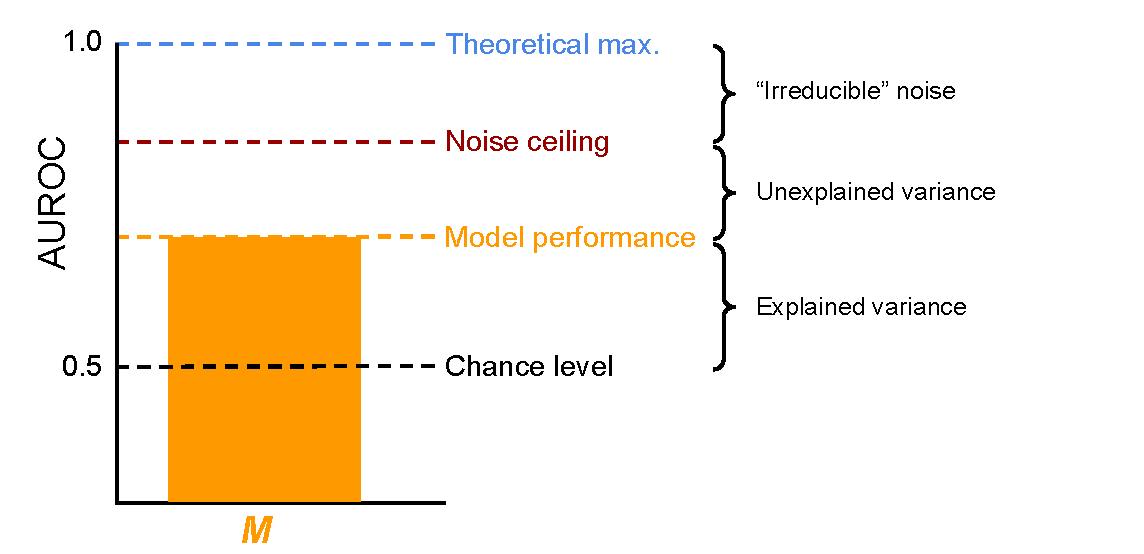
\includegraphics{_bookdown_files/hypothesis-kernel-analysis-files/figures/figure_3.pdf}
\caption{\label{fig:fig-hka-3}The noise ceiling partitions the variance into \emph{explained variance}, \emph{unexplained variance}, and \emph{``irreducible'' noise} for any given model (\(\mathbf{M}\)). Here, AUROC is used as the metric of model performance, but the noise ceiling can be estimated using any metric.}
\end{figure}



In the context of the current study, we use the variance (or ``inconsistency'') in emotion ratings across participants in response to the same set of facial expression stimuli to estimate a noise ceiling for the different AU-based models. The noise ceiling gives us insight into whether the evaluated set of AU-based models are sufficiently accurate to explain variance that can in principle be explained by AUs or whether we may need differently parameterized AU-based models. This way, the importance and limitations of AUs can be estimated empirically.

\hypertarget{evaluated-mappings}{%
\subsection{Evaluated mappings}\label{evaluated-mappings}}

Many different AU-emotion mappings have been put forward, but in this study we assess those summarized in Barrett et al. (\protect\hyperlink{ref-Barrett2019-bc}{2019}) (Table 1). Additionally, we included the AU-emotion mappings from the ``emotional FACS'' (EMFACS) manual (Friesen \& Ekman, \protect\hyperlink{ref-Friesen1983-ft}{1983}). So, in total, we evaluated six hypothesized AU-emotion mappings, which are summarized in Table \ref{tab:tab-hka-1} (and an additional data-driven AU-emotion mapping, see below).

\newpage
\pagestyle{empty}
\blandscape

\begingroup\fontsize{7}{9}\selectfont

\begin{ThreePartTable}
\begin{TableNotes}[para]
\item \textit{Note: } 
\item Mappings evaluated in the current study. The mappings from Darwin (1872) were taken from Matsumoto et al. (2018). Both the “reference configuration” (ref.) and the “international core pattern” (ICP) from Cordaro et al. (2018) are included. The + symbol means that AUs occur together. AUs following a comma represent optional AUs. The inverted \textasciicircum{} symbol represents “or”. When multiple configurations are explicitly proposed for a given emotion (i.e., a “many-to-one” mapping), they are represented as separate bullet points.
\end{TableNotes}
\begin{longtabu} to \linewidth {>{\raggedright\arraybackslash}p{4em}>{\raggedright}X>{\raggedright\arraybackslash}p{10em}>{\raggedright}X>{\raggedright}X>{\raggedright}X>{\raggedright}X>{\raggedright}X}
\caption{\label{tab:tab-hka-1}Evaluated AU-emotion mappings in our study}\\
\toprule
Emotion category & Darwin (1872) & EMFACS & Matsumoto et al. (2008) & Cordaro et al. (2018) - ref. & Cordaro et al. (2018) - ICP & Keltner et al. (2019) & Jack/Schyns\\
\midrule
\endfirsthead
\caption[]{\label{tab:tab-hka-1}Evaluated AU-emotion mappings in our study \textit{(continued)}}\\
\toprule
Emotion category & Darwin (1872) & EMFACS & Matsumoto et al. (2008) & Cordaro et al. (2018) - ref. & Cordaro et al. (2018) - ICP & Keltner et al. (2019) & Jack/Schyns\\
\midrule
\endhead

\endfoot
\bottomrule
\insertTableNotes
\endlastfoot
Anger & 4 + 5 + 24 + 38 & $\boldsymbol{\cdot}$ 4 + 5 + 7 + 10 + 22 + 23 + (25 $\lor$ 26) & 4 + (5 $\lor$ 7) + 22 + 23 + 24 & 4 + 5 + 7 + 23 & 4 + 7 & 4 + 7 & 4 + 5 + 17 + 23 +24\\
 &  & $\boldsymbol{\cdot}$ 4 + 5 + 7 + 10 + 23 + (25 $\lor$ 26) &  &  &  &  & \\
 &  & $\boldsymbol{\cdot}$ 4 + 5 + 7 + 17 + (23 $\lor$ 24) &  &  &  &  & \\
 &  & $\boldsymbol{\cdot}$ 4 + 5 + 7 + (23 $\lor$ 24) &  &  &  &  & \\
 &  & $\boldsymbol{\cdot}$ 4 + (5 $\lor$ 7) &  &  &  &  & \\
 &  & $\boldsymbol{\cdot}$ 17 + 24 &  &  &  &  & \\
Disgust & 10 + 16 + 22 + 25 + 26 & $\boldsymbol{\cdot}$ (9 $\lor$ 10) + 17 & (9 $\lor$ 10), (25 $\lor$ 26) & 9 + 15 + 16 & 4 + 6 + 7 + 9 + 10 + 25 + (26 $\lor$ 27) & 7 + 9 + 19 + 25 + 26 & 9 + 10 + 11 + 43\\
 &  & $\boldsymbol{\cdot}$ (9 $\lor$ 10) + 16 + (25 $\lor$ 26) &  &  &  &  & \\
 &  & $\boldsymbol{\cdot}$ (9 $\lor$ 10) &  &  &  &  & \\
Fear & 1 + 2 + 5 + 20 & $\boldsymbol{\cdot}$ 1 + 2 + 4 & 1 + 2 + 4 + 5 + 20, (25 $\lor$ 26) & 1 + 2 + 4 + 5 + 20 + 25 + 26 & 1 + 2 + 5 + 7 + 25 + (26 $\lor$ 27) & 1 + 2 + 4 + 5 + 7 + 20 + 25 & 4 + 5 + 20\\
 &  & $\boldsymbol{\cdot}$ 1 + 2 + 4 + 5 + 20 + (25 $\lor$ 26 $\lor$ 27) &  &  &  &  & \\
 &  & $\boldsymbol{\cdot}$ 1 + 2 + 4 + 5 &  &  &  &  & \\
 &  & $\boldsymbol{\cdot}$ 1 + 2 + =5 + (25 $\lor$ 26 $\lor$ 27) &  &  &  &  & \\
 &  & $\boldsymbol{\cdot}$ 5 + 20 + (25 $\lor$ 26 $\lor$ 27) &  &  &  &  & \\
 &  & $\boldsymbol{\cdot}$ 5 + 20 &  &  &  &  & \\
 &  & $\boldsymbol{\cdot}$ 20 &  &  &  &  & \\
Happiness & 6 + 12 & $\boldsymbol{\cdot}$ 12 & 6 + 12 & 6 + 12 & 6 + 7 + 12 + 16 + 25 + (26 $\lor$ 27) & 6 + 7 + 12 + 25 + 26 & 6 + 12 + 13 + 14 +25\\
 &  & $\boldsymbol{\cdot}$ 6 + 12 &  &  &  &  & \\
Sadness & 1 + 15 & $\boldsymbol{\cdot}$ 1 + 4 & 1 + 15, 4, 17 & 1 + 4 + 5 & 4 + 43 & 1 + 4 + 6 + 15 + 17 & 4 + 15 + 17 + 24 + 43\\
 &  & $\boldsymbol{\cdot}$ 1 + 4 + (11 $\lor$ 15) &  &  &  &  & \\
 &  & $\boldsymbol{\cdot}$ 1 + 4 + 15 + 17 &  &  &  &  & \\
 &  & $\boldsymbol{\cdot}$ 6 + 15 &  &  &  &  & \\
 &  & $\boldsymbol{\cdot}$ 11 + 17 &  &  &  &  & \\
 &  & $\boldsymbol{\cdot}$ 1 &  &  &  &  & \\
Surprise & 1 + 2 + 5 + 25 + 26 & $\boldsymbol{\cdot}$ 1 + 2 + 5 + (26 $\lor$ 27) & 1 + 2 + 5 + (25 $\lor$ 26) & 1 + 2 + 5 + 26 & 1 + 2 + 5 + 25 + (26 $\lor$ 27) & 1 + 2 + 5 + 25 + 26 & 1 + 2 + 5 + 26 + 27\\
 &  & $\boldsymbol{\cdot}$ 1 + 2 + 5 &  &  &  &  & \\
 &  & $\boldsymbol{\cdot}$ 1 + 2 + (26 $\lor$ 27) &  &  &  &  & \\
 &  & $\boldsymbol{\cdot}$ 5 + (26 $\lor$ 27) &  &  &  &  & \\*
\end{longtabu}
\end{ThreePartTable}
\endgroup{}

\elandscape
\newpage
\pagestyle{\defstyle}

All of these mappings propose that a number of AUs must occur together to communicate a particular emotion. However, the comparison between them is complicated by the fact that not all of them posit a single, consistent set of AUs per emotion. First, some contain multiple sets, such as the EMFACS manual (Friesen \& Ekman, \protect\hyperlink{ref-Friesen1983-ft}{1983}) proposing that ``sadness'' can be expressed with AUs 1 + 4 or AUs 6 + 15. Second, some offer optional AUs for a set, such as Matsumoto et al. (\protect\hyperlink{ref-Matsumoto2008-qk}{2008}) proposing that ``sadness'' is associated with AUs 1 + 15 and optionally with AUs 4 and/or 17. Thirdly, some describe \emph{mutually exclusive} options of AUs for a set, such as Matsumoto et al. (\protect\hyperlink{ref-Matsumoto2008-qk}{2008}) proposing that ``surprise'' can be communicated with AUs 1 + 2 + 5 in combination with \emph{either} AU25 \emph{or} AU26.

We address this issue by explicitly formulating all possible AU configurations that communicate a particular emotion for each mapping. For example, Matsumoto et al.~(2008) propose that ``disgust'' is associated with AU 9 or 10 and, optionally, AU 25 or 26, which yields six different possible configurations (9; 10; 9 + 25; 9 + 26; 10 + 25; 10 + 26). The specific configurations for each emotion derived from each evaluated mapping can be viewed in the study's code repository (in \texttt{mappings.py}; see \protect\hyperlink{hka-code}{Code Availability} section). In our analysis framework, we deal with multiple configurations per emotion (within a particular mapping), for each prediction separately, by using the configuration with the largest similarity to the stimulus under consideration (which occurs in between steps 3 and 4 in Figure \ref{fig:fig-hka-2}). We demonstrate that this procedure does not give an unfair advantage to mappings with more configurations using a simulation analysis (see Supplementary Figure \ref{fig:fig-hka-S4}).

In addition to evaluating existing mappings from the literature, we also constructed a mapping based on a data-driven analysis of the relationship between the AUs and emotion ratings from the dataset we use to evaluate the mappings. Importantly, to avoid circularity in our data-driven analysis (``double dipping''; Kriegeskorte et al., \protect\hyperlink{ref-kriegeskorte2009circular}{2009}), we performed the mapping estimation and evaluation on different partitions of the data (i.e., cross-validation). Specifically, we estimated the mapping on approximately 50\% of the trials from 50\% of the participants (the ``train set'') and evaluated the mapping on the other 50\% of trials from the other 50\% of the participants (the ``test set''). Importantly, the train and test set contained unique facial expressions and unique face identities, thus effectively treating both subject and stimulus as a random effect (Westfall et al., \protect\hyperlink{ref-westfall2016fixing}{2016}).

To estimate the data-driven mapping, we followed the procedure specified in Yu et al. (\protect\hyperlink{ref-Yu2012-ag}{2012}). For each AU and emotion, we computed the Pearson correlation between the binary activation values (1 if active, 0 otherwise) and the binary emotion rating (1 if this emotion was rated, 0 otherwise) for each participant in the train set. The raw correlations were averaged across the participants and binarized based on whether the correlation was statistically significant at \(\alpha = 0.05\) (1 if significant, 0 otherwise; uncorrected for multiple comparisons), which resulted in a binary 6 (emotion) × 33 (AU) mapping matrix.

\hypertarget{hka-dataset}{%
\subsection{Dataset used to evaluate mappings}\label{hka-dataset}}

We use data from an existing dataset (Yu et al., \protect\hyperlink{ref-Yu2012-ag}{2012}) which contains emotion ratings in response to 2400 dynamic facial expressions (with a duration of 1.25 seconds) with random AU configurations from 60 subjects. Each stimulus was composed of one of eight ``base faces'' and a random number of activated AUs drawn from a set of 42 AUs. Per stimulus, the number of AUs was drawn from a binomial distribution with parameters \(n = 6\) and \(p = 0.5\). The selected AUs varied in amplitude from 0 (not activated) to 1 (fully activated) in steps of 0.25 and a set of temporal parameters which determined the exact time course of each AU (see for details Yu et al., 2012). The original set of 42 AUs contained both compound AUs (such as AU25-12 and AU1-2) and AUs that could be activated both unilaterally (left or right) and bilaterally (such as AU12). In order to encode these AUs into independent variables, we recoded the compound AUs (e.g., activation of AU1-2 was recoded as activation of both AU1 and AU2) and bilateral AUs (e.g., activation of AU12 was recoded as activation of both AU12L and AU12R), yielding a total of 33 AUs: 1, 2L, 2R, 4, 5, 6L, 6R, 7L, 7R, 9, 10L, 10R, 11L, 11R, 12L, 12R, 13, 14L, 14R, 15, 16, 17, 20L, 20R, 22, 23, 24, 25, 26, 27, 38, 39, 43 (where L = left, R = right).

The emotion ratings were collected in a 7 alternative forced-choice facial expression categorization task in which participants were instructed to label the stimuli using one of the six universal basic emotions (``anger'', ``disgust'', ``fear'', ``happiness'', ``sadness'', and ``surprise) or, when the stimulus matched none of the emotion categories, ``other''. In addition, participants rated the ``intensity'' of the perceived emotion, which ranged from 1 (not intense at all) to 5 (very intense). Trials in which the stimulus was rated as ``other'' were removed from the dataset (because the evaluated mappings do not contain hypotheses about this category) leaving a grand total of 121,902 trials (average per subject: 2031.7 trials, \emph{SD}: 311.5) for our analysis. This grand total contains 4660 repeated observations with an average of 26.16 (\emph{SD}: 14.92) repetitions.

\hypertarget{hka-code}{%
\subsection{Code availability}\label{hka-code}}

All code used for this study's analysis and visualization of results is publicly available from Github: \url{https://github.com/lukassnoek/hypothesis-kernel-analysis}. The analyses were implemented in the Python programming language (version 3.7) and use several third-party packages, including \emph{numpy} (Harris et al., \protect\hyperlink{ref-Harris2020-en}{2020}), \emph{pandas} (McKinney \& Others, \protect\hyperlink{ref-McKinney2011-kl}{2011}), \emph{scikit-learn} (Pedregosa et al., \protect\hyperlink{ref-pedregosa2011scikit}{2011}), and \emph{seaborn} (Waskom, \protect\hyperlink{ref-waskom2021seaborn}{2021}). A Python package to compute noise ceilings as described in the current study can be found on Github: \url{https://github.com/lukassnoek/noiseceiling}.

\hypertarget{hka-results}{%
\section{Results}\label{hka-results}}

\hypertarget{prediction}{%
\subsection{Prediction}\label{prediction}}

In the first step of the modelling cycle, we evaluated how well each hypothesized AU-emotion mapping could \emph{predict} categorical emotion rating behavior in human participant. To do so, we developed a method to convert hypotheses about mappings between AUs and emotions into predictive models (see \protect\hyperlink{hka-methods}{Methods}). We then evaluated these models on their ability to predict categorical emotion labels from a psychophysics task containing a large set of dynamic facial expressions with random AU configurations. For each of the sixty observers, we summarized how well each model predicted the categorical emotion ratings using the Area Under the Receiver Operating Curve (AUROC), a metric with a chance level of 0.5 (which represents a model that randomly guesses the labels) and a theoretical maximum score of 1 (which represents a model that predicts each label perfectly). We additionally estimated a noise ceiling for each emotion, which represents an estimate of the maximum achievable model performance given the individual differences in ratings across participants (see \protect\hyperlink{methods}{Methods}). The logic behind a noise ceiling is that a single fixed model cannot capture any difference in emotion ratings across participants. The theoretical maximum performance (i.e.~an AUROC of 1) implies that different participants categorize the same combinations of AUs with the same emotion labels. However, if different individuals use different emotion labels for the same combinations of AUs, then this experimental noise will be irreducible, in turn reducing the noise ceiling and the proportion of variance that the models can possibly explain.

The results of the predictive analysis are summarized in Figure \ref{fig:fig-hka-4}, which shows the average and participant-specific AUROC scores separately for each mapping and emotion. The dashed line indicates each model's noise ceiling. The results indicate that almost all mappings predict each emotion well above chance level (i.e., an AUROC of 0.5), although substantial differences exist between different models and emotions. However, average model performance (i.e.~across mappings and emotions, with AUROC = 0.68) is still far from the average noise ceiling (i.e., an AUROC of 0.87). This indicates that the models tested do not perform optimally. Finally, considering that optimal performance is an AUROC of 1.0, substantially lower noise ceilings in this experiment indicates that a large proportion of the variability of emotion categorizations across participants cannot, in principle, be explained by any of the evaluated models.

\begin{figure}
\centering
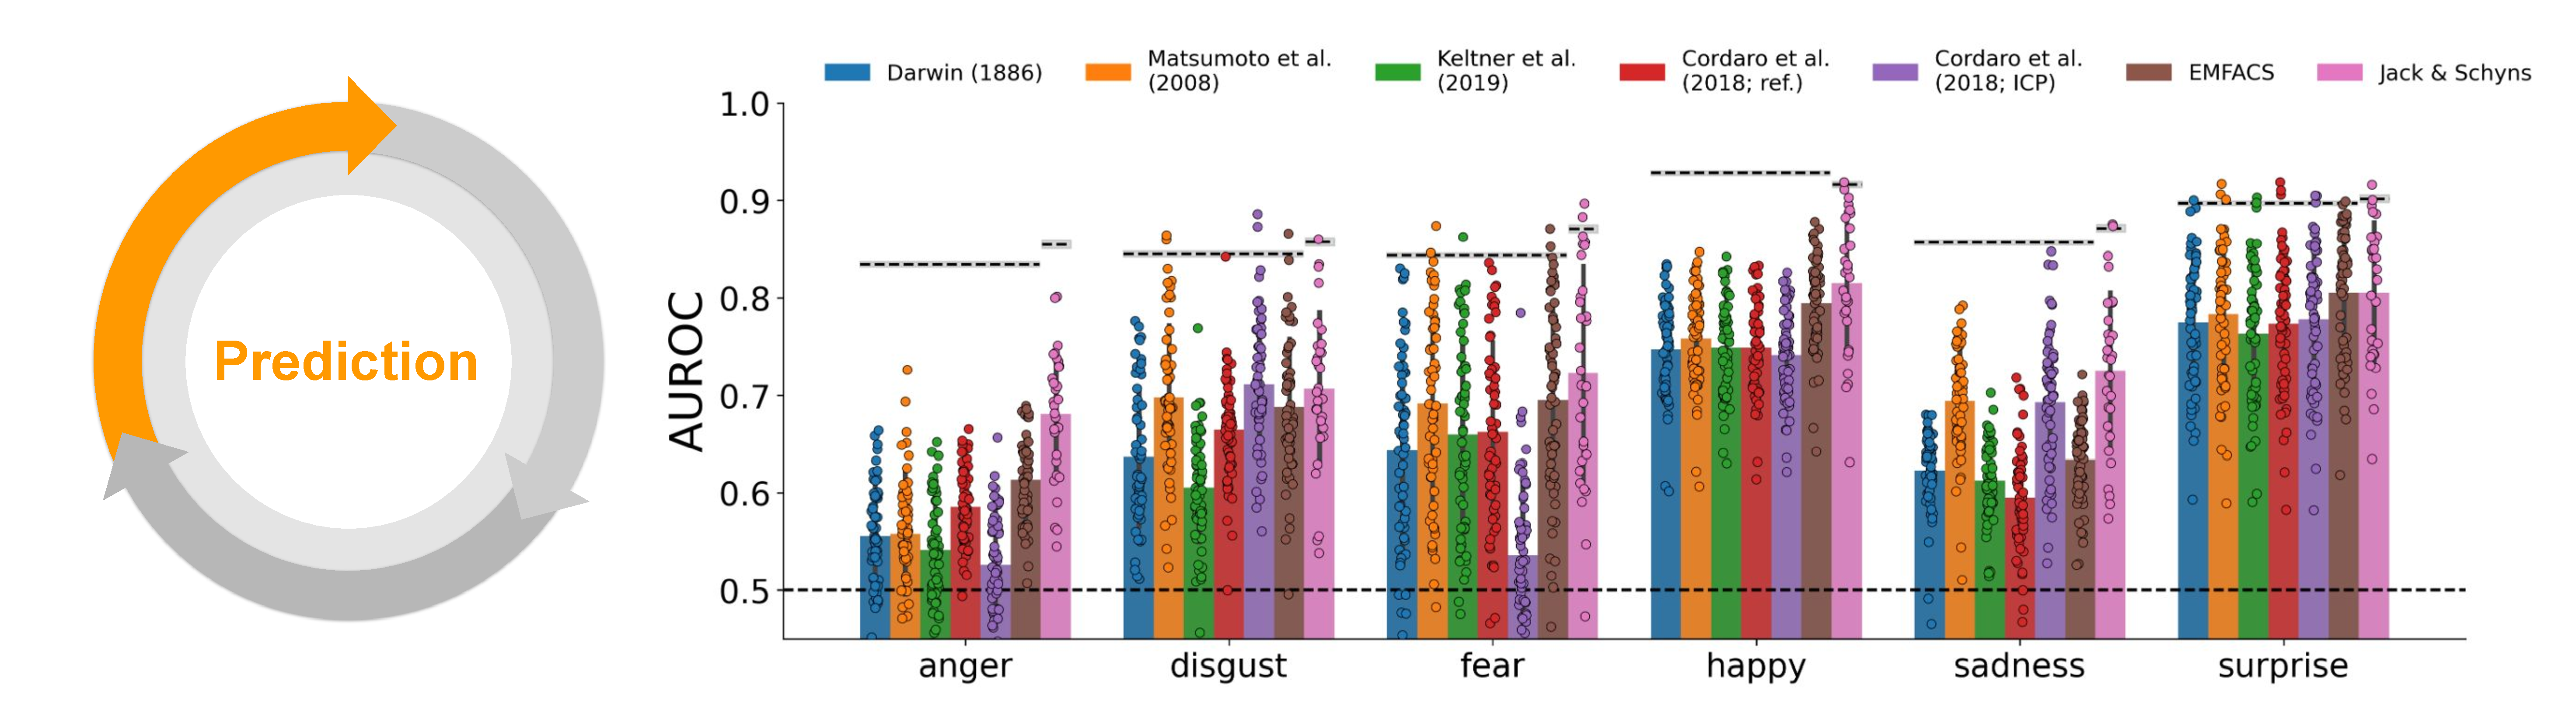
\includegraphics{_bookdown_files/hypothesis-kernel-analysis-files/figures/figure_4.pdf}
\caption{\label{fig:fig-hka-4}\emph{Prediction}. AUROC scores for each mapping (different bars), shown separately for each emotion (x-axis). Dots indicate individual participants. Dashed line and value directly above represent the noise ceiling (gray area represents ± 1 SD based on bootstrapping the repeated observations). The slightly different noise ceiling for Jack \& Schyns results from using half of the participants for evaluation.}
\end{figure}



\hypertarget{explanation}{%
\subsection{Explanation}\label{explanation}}

In the second step of the modelling cycle, we \emph{explained} the predictions and relative accuracy of the different mappings by quantifying the effect of each AU on model performance using an ``ablation analysis''. We systematically manipulated each model by selectively removing (or ``ablating'') each AU from each emotion combination and then reran the predictive analysis (see Figure \ref{fig:fig-hka-5}). The difference in model performance between the original (non-ablated) and ablated models indicates how important the ablated AU is for each categorizing each emotion. Specifically, if ablating an AU decreases performance for a particular emotion, it implies that participants tend to associate this AU with this particular emotion (and vice versa).

\begin{figure}
\centering
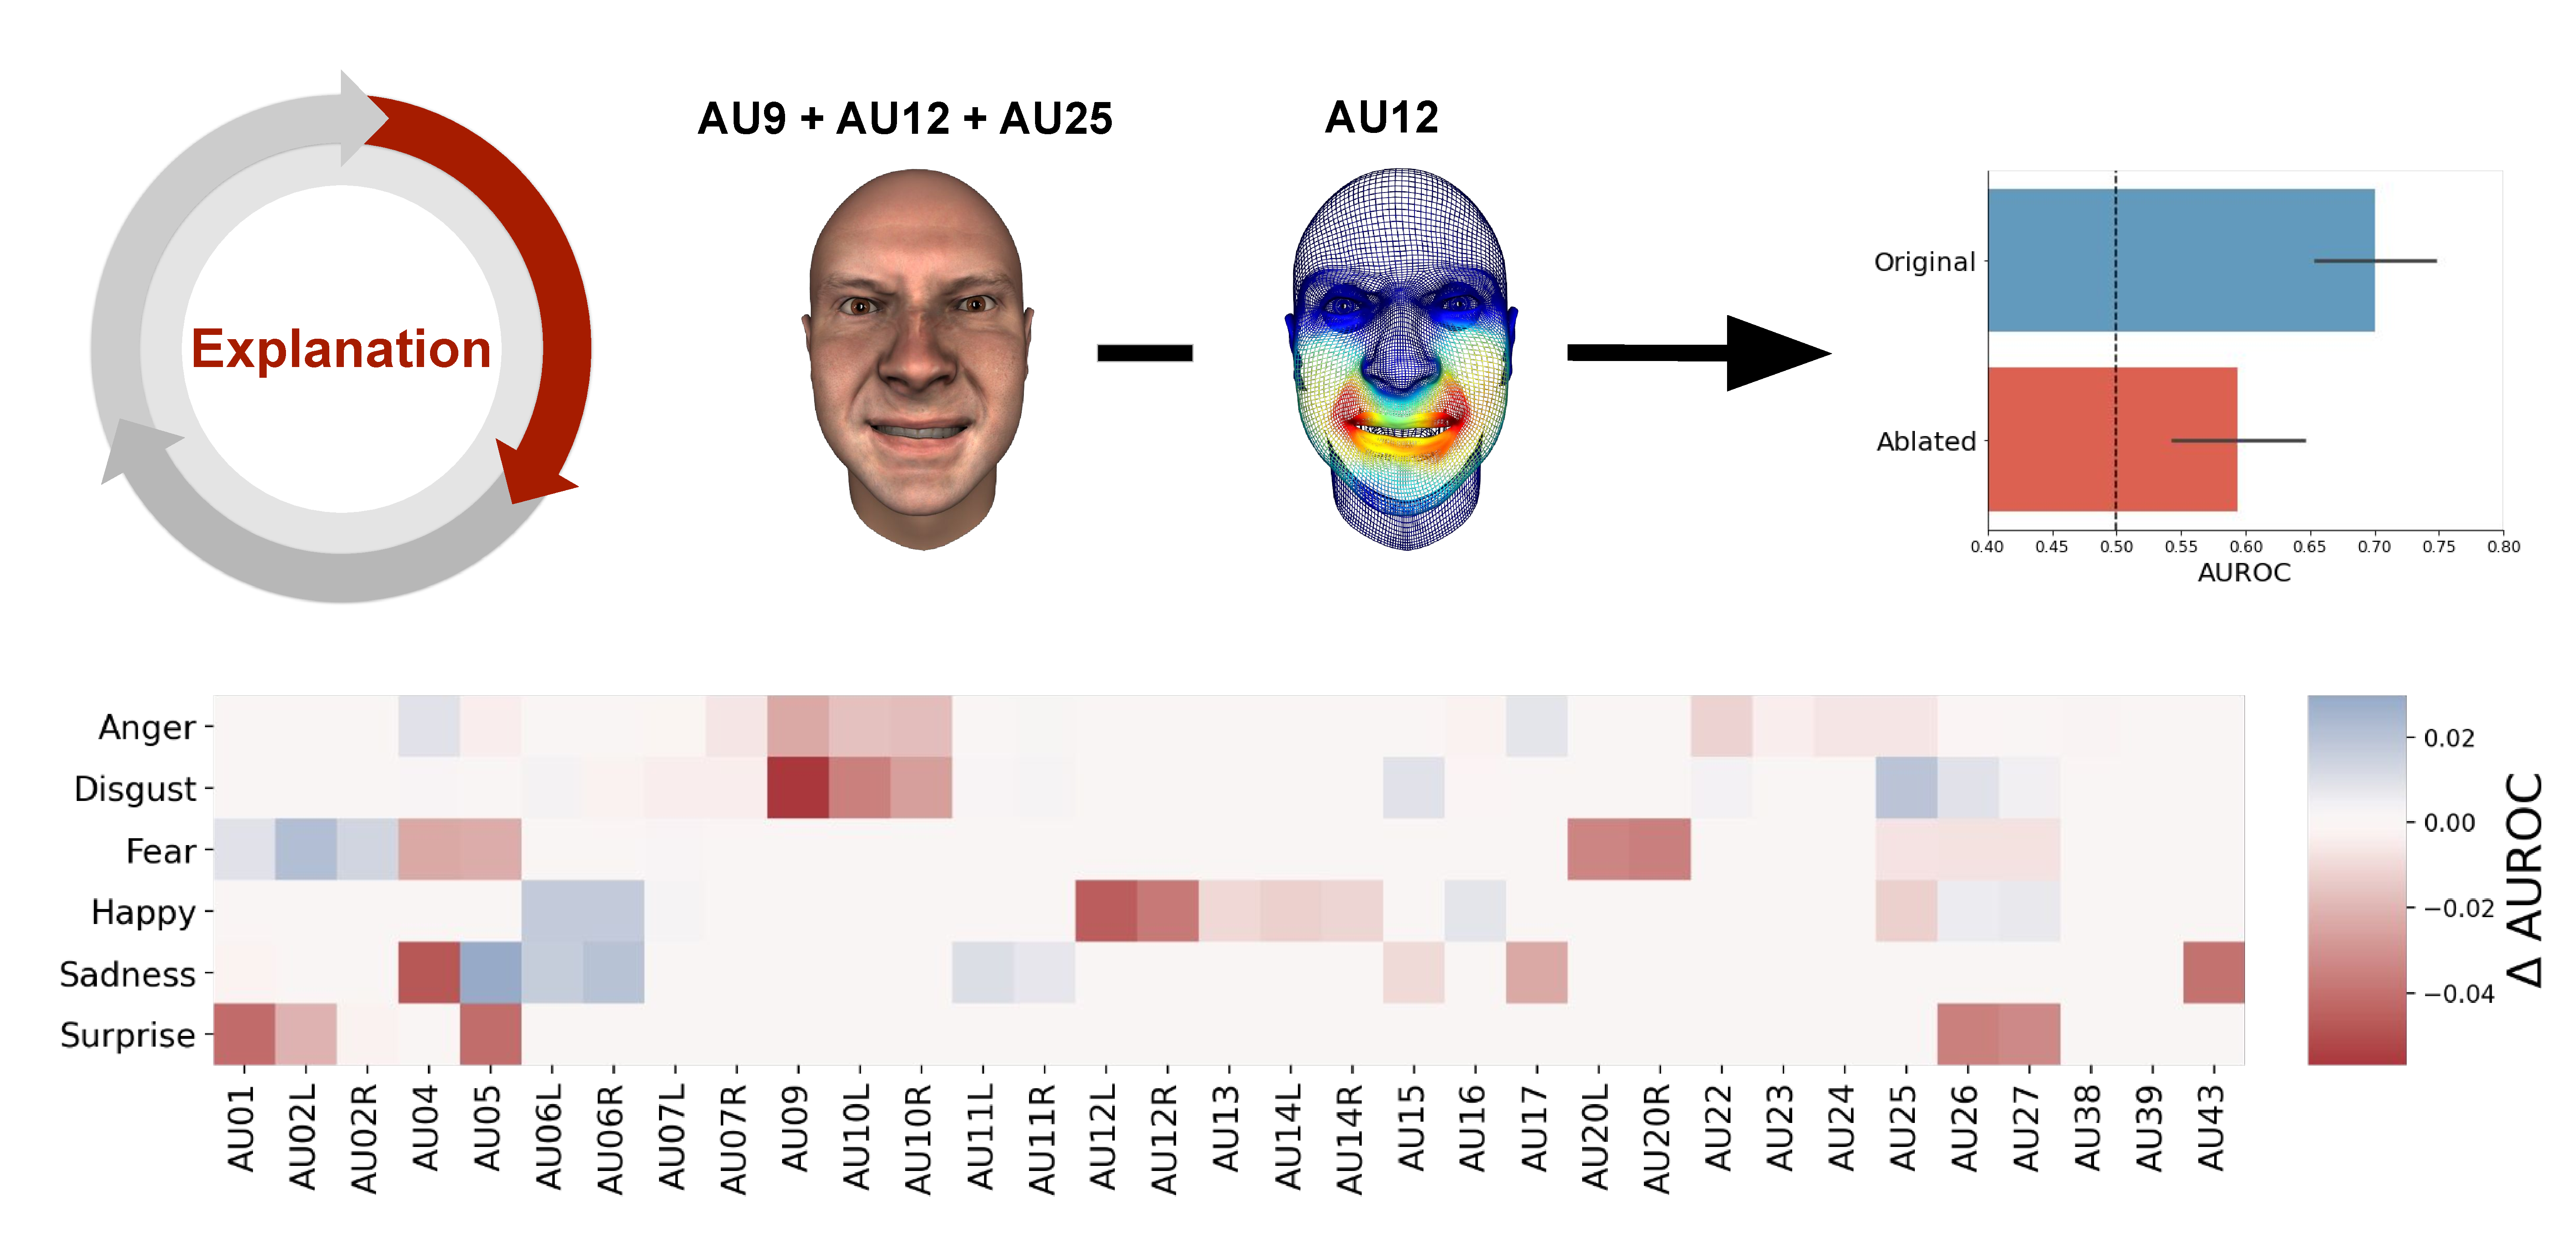
\includegraphics{_bookdown_files/hypothesis-kernel-analysis-files/figures/figure_5.pdf}
\caption{\label{fig:fig-hka-5}\emph{Explanation}. Schematic visualization of the explanation process through ablation of single AUs. The heatmap shows the average decrease (red) or increase (blue) across mappings after ablation of a single AU (x-axis) from a particular emotion configuration (y-axis).}
\end{figure}



The heatmap in Figure \ref{fig:fig-hka-5} shows how ablation of each AU impacts the model performance for each emotion, averaged across each combination that contains that particular AU (for the results per mapping, see Supplementary Table \ref{tab:tab-hka-S1} and Supplementary Figure \ref{fig:fig-hka-S5}). These results reveal both AUs that decrease performance when ablated (e.g., AU9 for disgust and AU5 for surprise) and AUs that increase performance when ablated (e.g., AU5 for sadness). Importantly, these results suggest that models can potentially be improved by selectively adding or removing these informative AUs (e.g., adding AU9 to Darwin's disgust mapping and removing AU5 from Cordaro et al.~- ref).

\hypertarget{exploration}{%
\subsection{Exploration}\label{exploration}}

In the third step of the modelling cycle, we used the results from the ablation analysis to \emph{explore} alternative, optimized mappings between AUs and emotions. We created optimized models by enhancing mappings with \emph{all} AUs that led to a decrease in model performance after ablation (i.e., all ``red'' cells in the heatmap from Figure \ref{fig:fig-hka-5}) and removing AUs from mappings that led to an increase in model performance after ablation (i.e., all ``blue'' cells in the heatmap from Figure \ref{fig:fig-hka-5}). Figure 4 (top) shows the difference in model performance between the original and the optimized model. Model performance improved substantially for almost all mappings and emotions, with anger improving the most (median improvement in AUROC: 0.13) and surprise the least (median improvement in AUROC: 0.03). However, all emotions were predicted well below the noise ceiling: the difference between the noise ceiling and optimal model performance ranged from 0.08 for happiness and 0.13 for sadness categorizations (for details, see Supplementary Figure \ref{fig:fig-hka-S6}).

In addition, we investigated how the optimized models led to behaviors different from the original models, by computing their corresponding confusion matrix, which shows how a model misclassifies trials. An ideal model will have a confusion matrix with off-diagonal values of zero indicating no confusion. Figure \ref{fig:fig-hka-6} shows that the original models frequently confused anger with disgust and disgust with happiness. The optimized models substantially reduced these confusions. To quantify this reduction, we computed percentage difference of misclassified trials (i.e., the off-diagonal values of the confusion matrix) between the optimized and original model, which ranged between 2.2\% (Jack \& Schyns) and 12.2\% (Darwin, 1886).

\begin{figure}
\centering
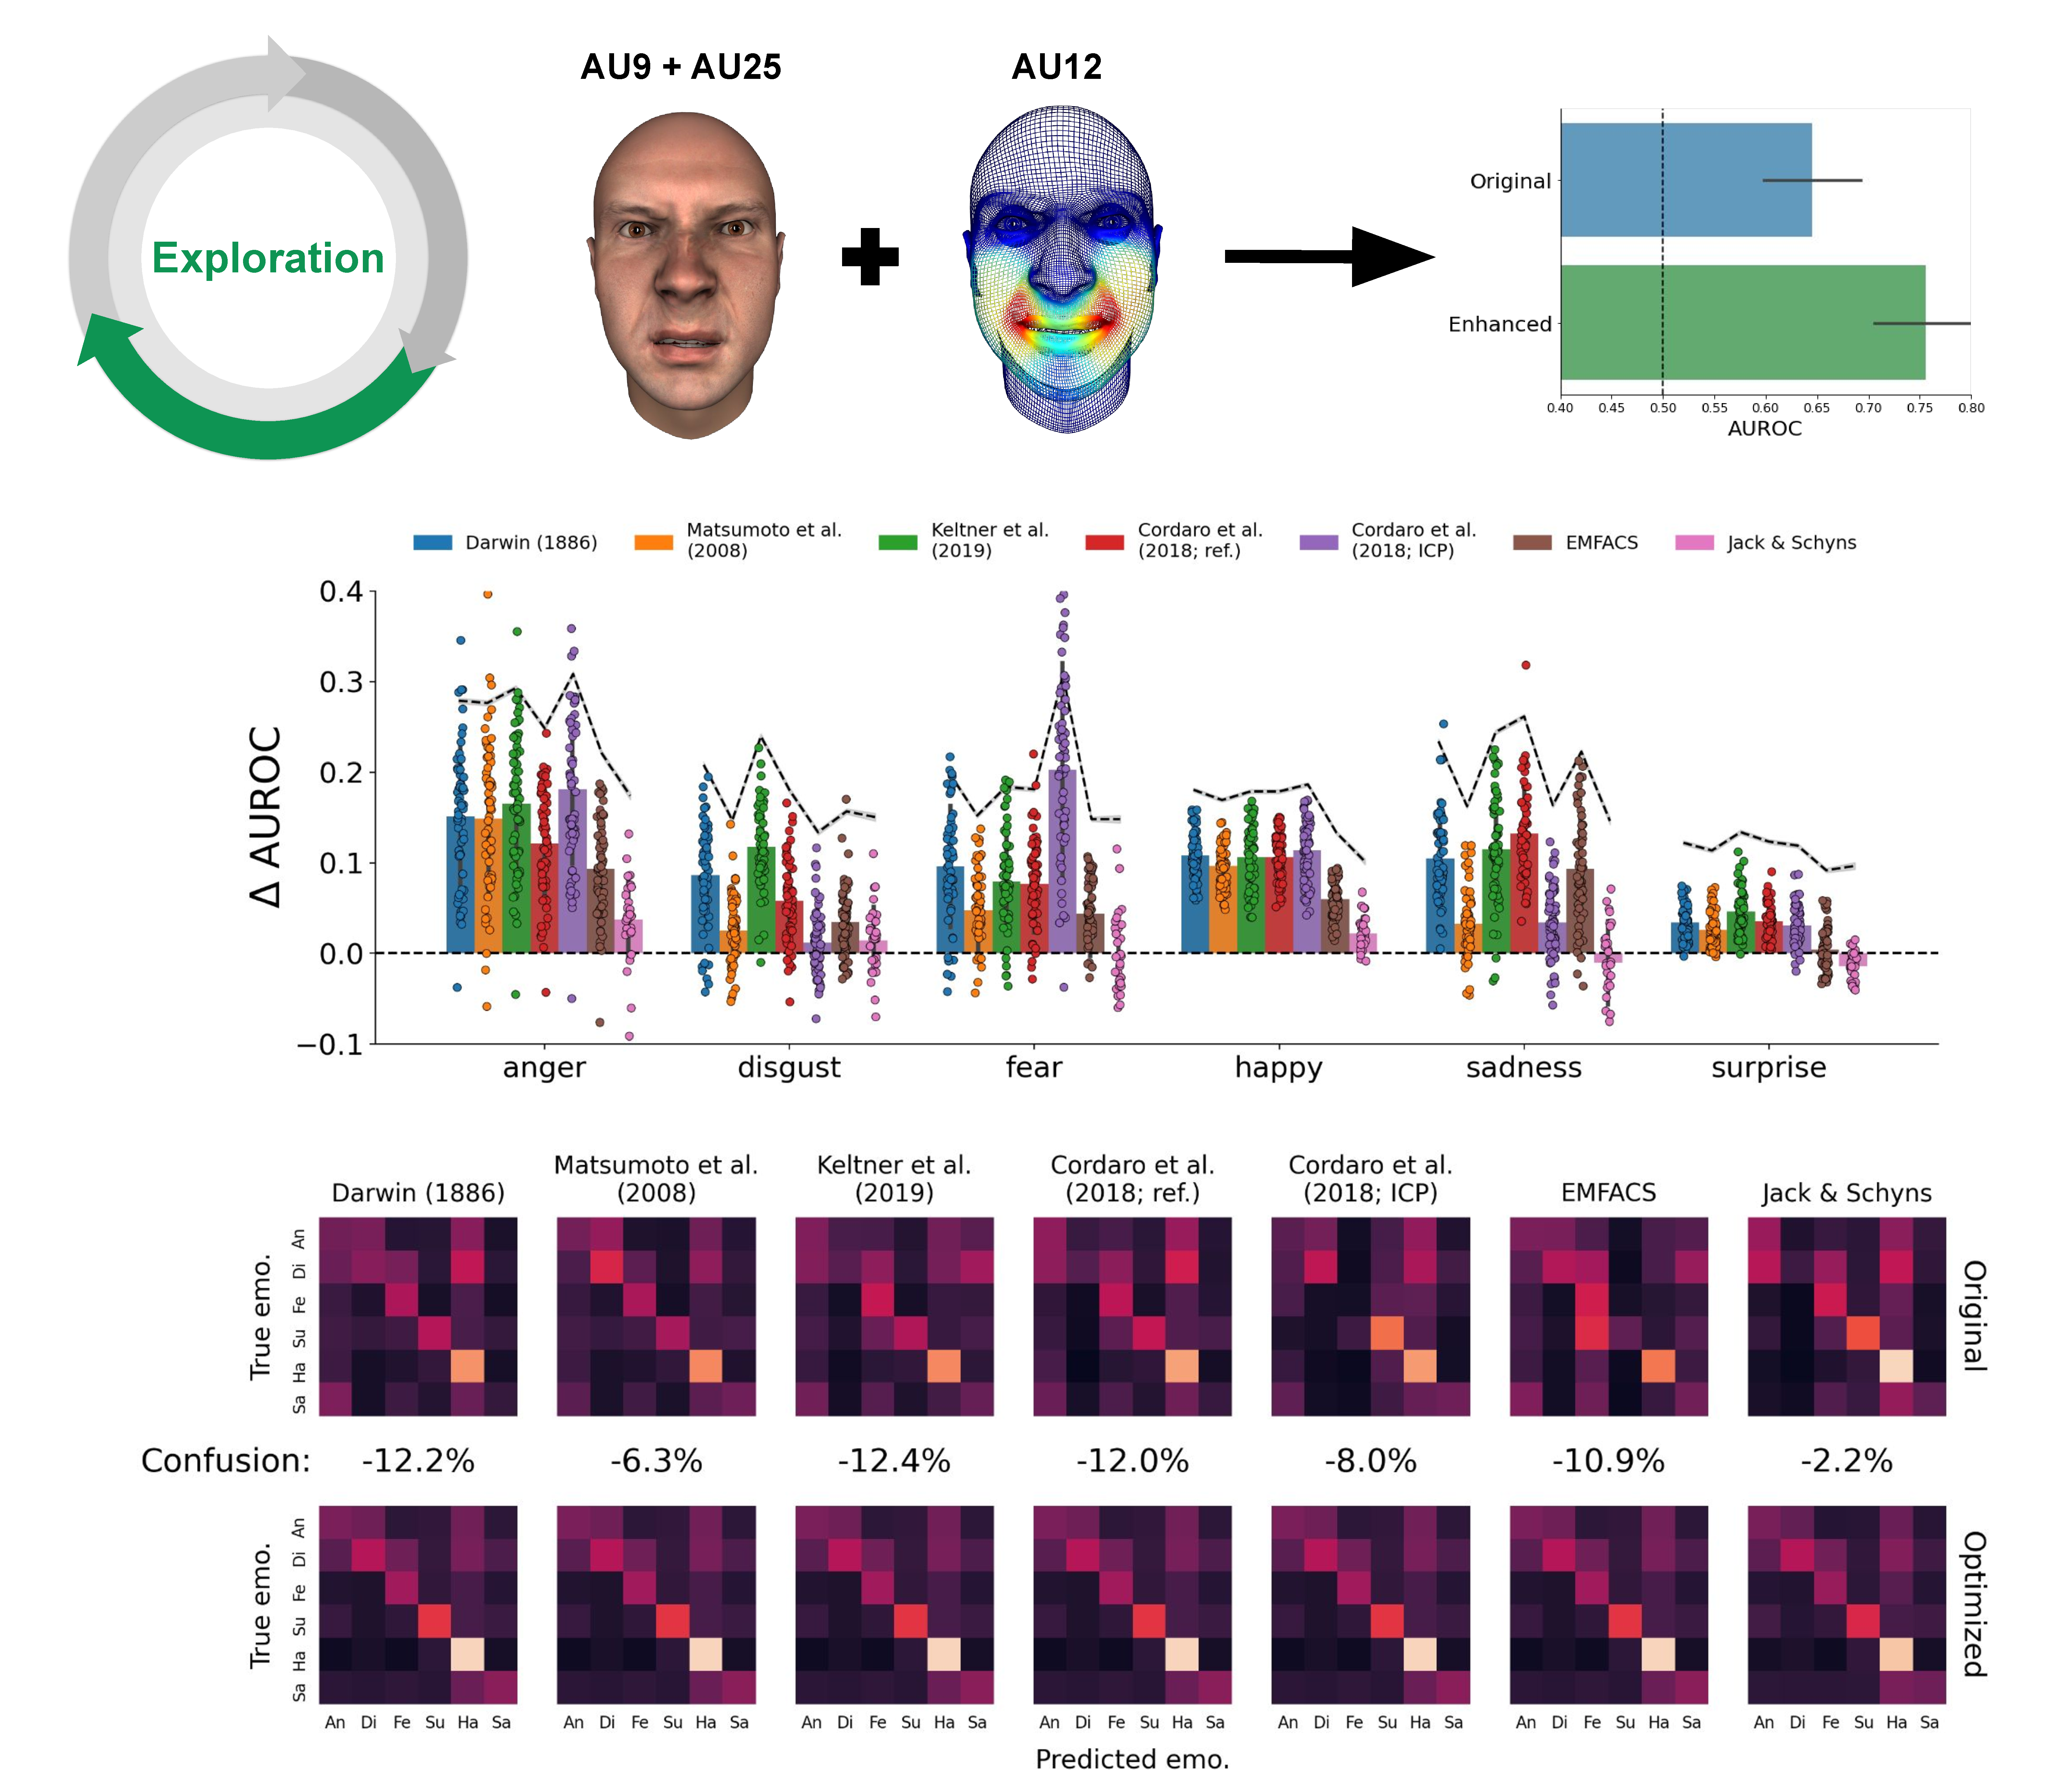
\includegraphics{_bookdown_files/hypothesis-kernel-analysis-files/figures/figure_6.pdf}
\caption{\label{fig:fig-hka-6}\emph{Exploration}. Schematic visualization of the exploration process through enriching existing models with additional AUs. Bar graph shows the change in model performance (\$Delta\$ AUROC) of the optimal model relative to the original model (cf.~Figure \ref{fig:fig-hka-4}). The dashed line represents the original noise ceiling. Bottom: confusion matrices (normalized by the sum across rows, indicating sensitivity) of the original and optimized model and reduction in confusion rate.}
\end{figure}



\hypertarget{hka-discussion}{%
\section{Discussion}\label{hka-discussion}}

Since Darwin's seminal work on the evolutionary origins of emotional expressions, a debate has centered on the question of the specific combinations of facial movements that consistently expressed different emotions. The influential taxonomy of facial movements as AUs proposed by Ekman \& Friesen (\protect\hyperlink{ref-Ekman1976-hm}{1976}) enabled different hypotheses to be formulated about the specific combinations of action units that underlie the expression and recognition of emotion categories.

In this study, we developed this approach further, by formalizing these proposals for combinations of AUs as predictive models of human categorization behavior. We used these formal models to quantitatively evaluate how well each model \emph{predicts} the categorization of emotions. We then \emph{explained} the differences in predictive accuracy with systematic manipulations of the AUs comprising each model. In turn, this generated insights that enabled \emph{exploration} of alternative and improved models. Moreover, we showed that models were inherently limited in their prediction of human behavior, due to individual differences in how people perceive facial expressions.

With our model-based approach, we could precisely quantify specifically how much different AU-emotion mappings predicted emotion categorizations. We found that all models could predict a substantial proportion of the variance, but with pronounced differences between models. The ablation analysis indicated that these differences could be explained by AUs beneficial for prediction that were lacking in some models, and also that other models comprised AUs that in fact hindered their predictions. We used these insights to explore alternative, ``optimized'' models that, in turn, substantially improved predictive accuracy. This prediction-explanation-exploration cycle demonstrates that a model-based approach offers a detailed summary of the strengths and limitations of the evaluated models and therefore enables their improvements.

An important advantage of formal models is we can use their predictive accuracy to quantify within a common metric how much of a cognitive capacity is accounted for, and how much is not. To better understand the limits of the evaluated models, we computed their noise ceiling. This partitions the gap between the actual and maximal model performance into the \emph{unexplained variance} and that due to \emph{individual differences} (see Figure \ref{fig:fig-hka-3}). The noise ceiling uses the individual variations in individuals that categorize a given model to estimate an upper bound of the model performance. Variance below the noise ceiling is consistent across individuals and can thus, in principle, be explained by a single, fixed model. In contrast, variance above the noise ceiling represents individual differences (e.g., participant 1 rates stimulus \(X\) as ``anger'' while participant 2 rates it as ``disgust'') which is impossible to explain by a single, fixed model.

Our results indicate that the evaluated models, including in their optimized forms, do not reach the noise ceiling, implying that they likely lack important information. Future research could improve these models so they may reach the noise ceiling. One possibility is to ``weigh'' the AUs in each model (to weight their importance, or probability), instead of having ``binary'' AUs (i.e.~either ``on'' or ``off'') as is often the norm. Also, facial expressions are inherently dynamic, so incorporating their temporal information could also improve their categorization (Delis et al., \protect\hyperlink{ref-Delis2016-zl}{2016}; Jack et al., \protect\hyperlink{ref-Jack2014-ku}{2014}).

The observation that the evaluated models are strongly limited by the observed individual differences in emotion ratings begs the question what underlies these individual differences. In the context of the current study, individual differences could include any factor that differs between individuals, including age, sex, personality and culture of the perceiver \&mdash all of which have been shown to influence the association between AUs and emotions (Jack et al., \protect\hyperlink{ref-Jack2012-eq}{2012}; Parmley \& Cunningham, \protect\hyperlink{ref-Parmley2014-nj}{2014}). Incorporating these factors in the models or constructing separate models for different groups (e.g., for different cultures) could account for the individual differences that would otherwise contribute to noise.

In sum, our model-based approach allowed us to systematically test previously hypothesized mappings between AUs and emotion categories, which we found explain a substantial proportion of variance in emotion categorizations, but remain limited by individual differences. These question the possibility of a universal model of emotional facial expressions. We propose that future studies investigate the specific factors that cause individual differences to enable the development of more complete and accurate models of facial expressions of emotion.

\hypertarget{static-vs-dynamic}{%
\chapter{Affective face perception integrates both static and dynamic information}\label{static-vs-dynamic}}

\chaptermark{Static vs. dynamic}

\vspace*{\fill}

\begin{center}\rule{0.5\linewidth}{0.5pt}\end{center}

\newpage
\normalsize

\begin{abstract}
Facial movements are crucial for affective face perception, yet research has shown that people are also influenced by features of the static face such as facial morphology. Most studies have either manipulated dynamic features (i.e., facial movements) or static features (i.e., facial morphology) making it impossible to evaluate the relative contribution of either. The current study investigates the effects of static and dynamic facial features on three affective properties (categorical emotion, valence, and arousal) inferred from stimuli in which both types of features have been independently manipulated. Using predictive machine learning models, we show that static and dynamic features both explain substantial and orthogonal variance in categorical emotion and valence ratings, while arousal ratings are only predicted accurately using dynamic, but not static, features. Moreover, using a multivariate reverse correlation approach, we show that static and dynamic features communicating the same affective property (e.g., categorical emotions) are manifested differently in the face. Our results demonstrate that in order to understand affective face perception, both facial morphology and facial movements should be considered independently.
\end{abstract} \newpage

\hypertarget{svsd-introduction}{%
\section{Introduction}\label{svsd-introduction}}

Faces are an important element of our daily life; faces communicate affective states of others and elicit feelings in ourselves. We might infer that someone is happy when she raises the corners of her mouth and wrinkles her eyes and we might feel unpleasant when confronted with a disapproving frown. Faces convey such impressions through facial movements, which are thought to be the primary instrument to express and communicate affective states to others (Jack \& Schyns, \protect\hyperlink{ref-Jack2015-sh}{2015}). Nevertheless, most research on affective face perception has used static depictions of facial expressions in which only the peak of the expression is shown. As such, facial movements in static stimuli are not directly observed but have to be inferred. Furthermore, although facial movements are arguably the primary drivers of how we perceive and are affected by others' faces, studies have argued that facial movements alone are unlikely to capture all variation in how we perceive and are affected by others' faces (Barrett et al., \protect\hyperlink{ref-Barrett2019-bc}{2019}; Snoek et al., \protect\hyperlink{ref-snoek-submitted}{n.d.}). One possible additional source of information that may complement the dynamic information conveyed by facial movements is the static, or ``neutral'', face. Although the static face is unrelated to the expressor's affective state, studies have shown that features of the static face, such as facial morphology and complexion, in fact influence how we perceive and experience faces (Hess, Adams, \& Kleck, \protect\hyperlink{ref-Hess2009-xo}{2009}; Neth \& Martinez, \protect\hyperlink{ref-Neth2009-eh}{2009}). Although much research has examined both static features and dynamic features in the context of affective face perception (reviewed below), they have never been manipulated and compared using the same stimuli in the same experiment. In the current study, we seek to investigate, quantify, and disentangle the relative contribution of these static and dynamic facial features to affective face perception.

The attempts to relate specific facial movements to affective states go back as far as Charles Darwin's descriptions of stereotypical facial expressions associated with categorical emotions (Darwin, \protect\hyperlink{ref-Darwin1872-nv}{1872}). Since Darwin, more quantitative efforts have been made to establish robust associations between facial movements and affective states, and categorical emotions in particular. An important development that facilitated these efforts was the Facial Action Coding System (FACS; Ekman \& Friesen, \protect\hyperlink{ref-Ekman1976-hm}{1976}), which outlines a way to systematically measure, quantify, and categorize facial movements into components called ``action units'' (AUs). Using FACS, studies have investigated and proposed specific configurations of facial movements associated with affective states such as categorical emotions (Jack et al., \protect\hyperlink{ref-Jack2014-ku}{2014}, \protect\hyperlink{ref-Jack2012-eq}{2012}; Wegrzyn et al., \protect\hyperlink{ref-Wegrzyn2017-ke}{2017}), valence and arousal (Höfling et al., \protect\hyperlink{ref-Hofling2020-mk}{2020}; Liu et al., \protect\hyperlink{ref-Liu2020-vo}{2020}), and pain (Chen et al., \protect\hyperlink{ref-chen2018distinct}{2018}; Kunz et al., \protect\hyperlink{ref-Kunz2019-uh}{2019}; for a comprehensive overview, see Barrett et al., \protect\hyperlink{ref-Barrett2019-bc}{2019}). Moreover, advances in computer vision spurred the development of algorithms that are able to classify affective states based on action units (J. Cohn \& Kanade, \protect\hyperlink{ref-Cohn2007-xe}{2007}; Lien et al., \protect\hyperlink{ref-Lien1998-bg}{1998}) or other facial features such as facial landmarks (Toisoul et al., \protect\hyperlink{ref-Toisoul2021-yc}{2021}) or geometric features (Barman \& Dutta, \protect\hyperlink{ref-Barman2019-af}{2019}; Murugappan \& Mutawa, \protect\hyperlink{ref-Murugappan2021-yj}{2021}).

Despite the fact that facial features arguably need to be dynamic to communicate affective states, static morphological features of the face have been found to influence, or ``bias'', how people interpret others' faces. This claim is supported by research showing that people can perceive emotions in neutral (i.e., non-expressive) faces that by definition only contain static but no dynamic features. Such an effect has been demonstrated by manipulating structural features of neutral faces, where, for example, a neutral face with a lower nose and mouth or higher eyebrows was more likely to be perceived as sad (Neth \& Martinez, \protect\hyperlink{ref-Neth2009-eh}{2009}; see also Franklin et al., \protect\hyperlink{ref-Franklin2019-qo}{2019}). Similar effects have been observed in relation to certain demographics (gender, ethnicity, or age) or social judgements (e.g., dominance) that are associated with specific variations in facial morphology. For instance, research has shown that neutral male faces are more likely to be perceived as angry than neutral female faces (Adams et al., \protect\hyperlink{ref-Adams2016-tz}{2016}; Brooks et al., \protect\hyperlink{ref-Brooks2018-ao}{2018}; Craig \& Lipp, \protect\hyperlink{ref-Craig2018-jm}{2018}) and people perceive fewer and less intense emotions in older faces relative to younger faces (reviewed in Fölster et al., \protect\hyperlink{ref-Folster2014-zy}{2014}). The dominant explanation for these affective inferences from static faces is that these effects are driven by the visual resemblance of static features (e.g., a relatively low brow) to dynamic features associated with a particular affective state (e.g., lowering one's brow as part of an anger expression; Hess, Adams, \& Kleck, \protect\hyperlink{ref-Hess2009-xo}{2009}; Said et al., \protect\hyperlink{ref-Said2009-tf}{2009}; Zebrowitz, \protect\hyperlink{ref-Zebrowitz2017-qe}{2017}; but see Gill et al., \protect\hyperlink{ref-Gill2014-hx}{2014}; Guan et al., \protect\hyperlink{ref-Guan2018-hq}{2018}).

As discussed, many studies have investigated dynamic and static features that underlie affective face perception. However, because these studies usually manipulate either dynamic facial movements (Jack et al., \protect\hyperlink{ref-Jack2014-ku}{2014}, \protect\hyperlink{ref-Jack2009-yy}{2009}) \emph{or} static facial features (Franklin et al., \protect\hyperlink{ref-Franklin2019-qo}{2019}; Neth \& Martinez, \protect\hyperlink{ref-Neth2009-eh}{2009}; for an exception, see Gill et al., \protect\hyperlink{ref-Gill2014-hx}{2014}), the relative contribution of dynamic and static information remains unknown. In addition, studies investigating the effect of dynamic features (such as AUs) on affective face processing often use static stimuli (i.e., images; Krumhuber et al., \protect\hyperlink{ref-Krumhuber2013-qi}{2013}) which only shows the ``peak'' of the expression. The use of such static stimuli means facial movements are not directly visible and need to be inferred. As a consequence, in such studies the effect of dynamic and static features on affective face perception are fundamentally confounded. For example, a participant cannot know if a relatively low eyebrow is low because of a facial muscle movement or just because of the structure of the face. This potential confound of static features is even more problematic in automated facial emotion recognition systems, which often require static images as input (e.g., including the emotion recognition systems offered by Microsoft and Google\footnote{\url{https://azure.microsoft.com/en-us/services/cognitive-services/face}, \url{https://cloud.google.com/vision/docs/detecting-faces}}), which may inadvertently use static facial features associated with certain demographic groups (e.g., based on ethnicity or age, Xu et al., \protect\hyperlink{ref-Xu2020-jd}{2020}; Bryant \& Howard, \protect\hyperlink{ref-Bryant2019-sg}{2019}) leading to biased predictions. Moreover, the confounding influence of static features is especially problematic for the aforementioned hypothesis that static features important for affective face perception visually resemble corresponding dynamic features (Hess, Adams, Grammer, et al., \protect\hyperlink{ref-Hess2009-jz}{2009}; Hess, Adams, \& Kleck, \protect\hyperlink{ref-Hess2009-xo}{2009}; Said et al., \protect\hyperlink{ref-Said2009-tf}{2009}).

To overcome these limitations, the current study investigates the relative contribution of dynamic and static information to affective face perception (see Figure \ref{fig:fig-svsd-1}). To disentangle these two sources of information, we use a psychophysics approach that features video stimuli in which both the dynamic information (i.e., facial movements) and static information (i.e., facial morphology) is manipulated. In terms of affective properties, we focus on categorical emotions inferred by the observer in the expressor as well as valence and arousal elicited in the observer. Although these two concepts are fundamentally different (the former is an estimate of the affective state of the expressor while the latter two reflect the affective state of the observer), we investigate these properties to investigate how static and dynamic facial features affect both affective perception (categorical emotions) and affective experience (valence and arousal). We use machine learning models that predict human ratings of these affective properties based on dynamic and static information. Using this approach, which focuses on cross-validated predictive model performance rather than statistical significance (Yarkoni \& Westfall, \protect\hyperlink{ref-Yarkoni2017-om}{2017}), we are able to precisely quantify and compare the variance explained by static and dynamic features of the face. Finally, we implement a multivariate reverse correlation technique to reconstruct, visualize, and compare the mental representations of the facial features that underlie the information extracted and used by our static and dynamic models. This technique facilitates the interpretation of the commonalities and differences between static and dynamic facial features important for predicting categorical emotion, valence and arousal.

\begin{figure}
\centering
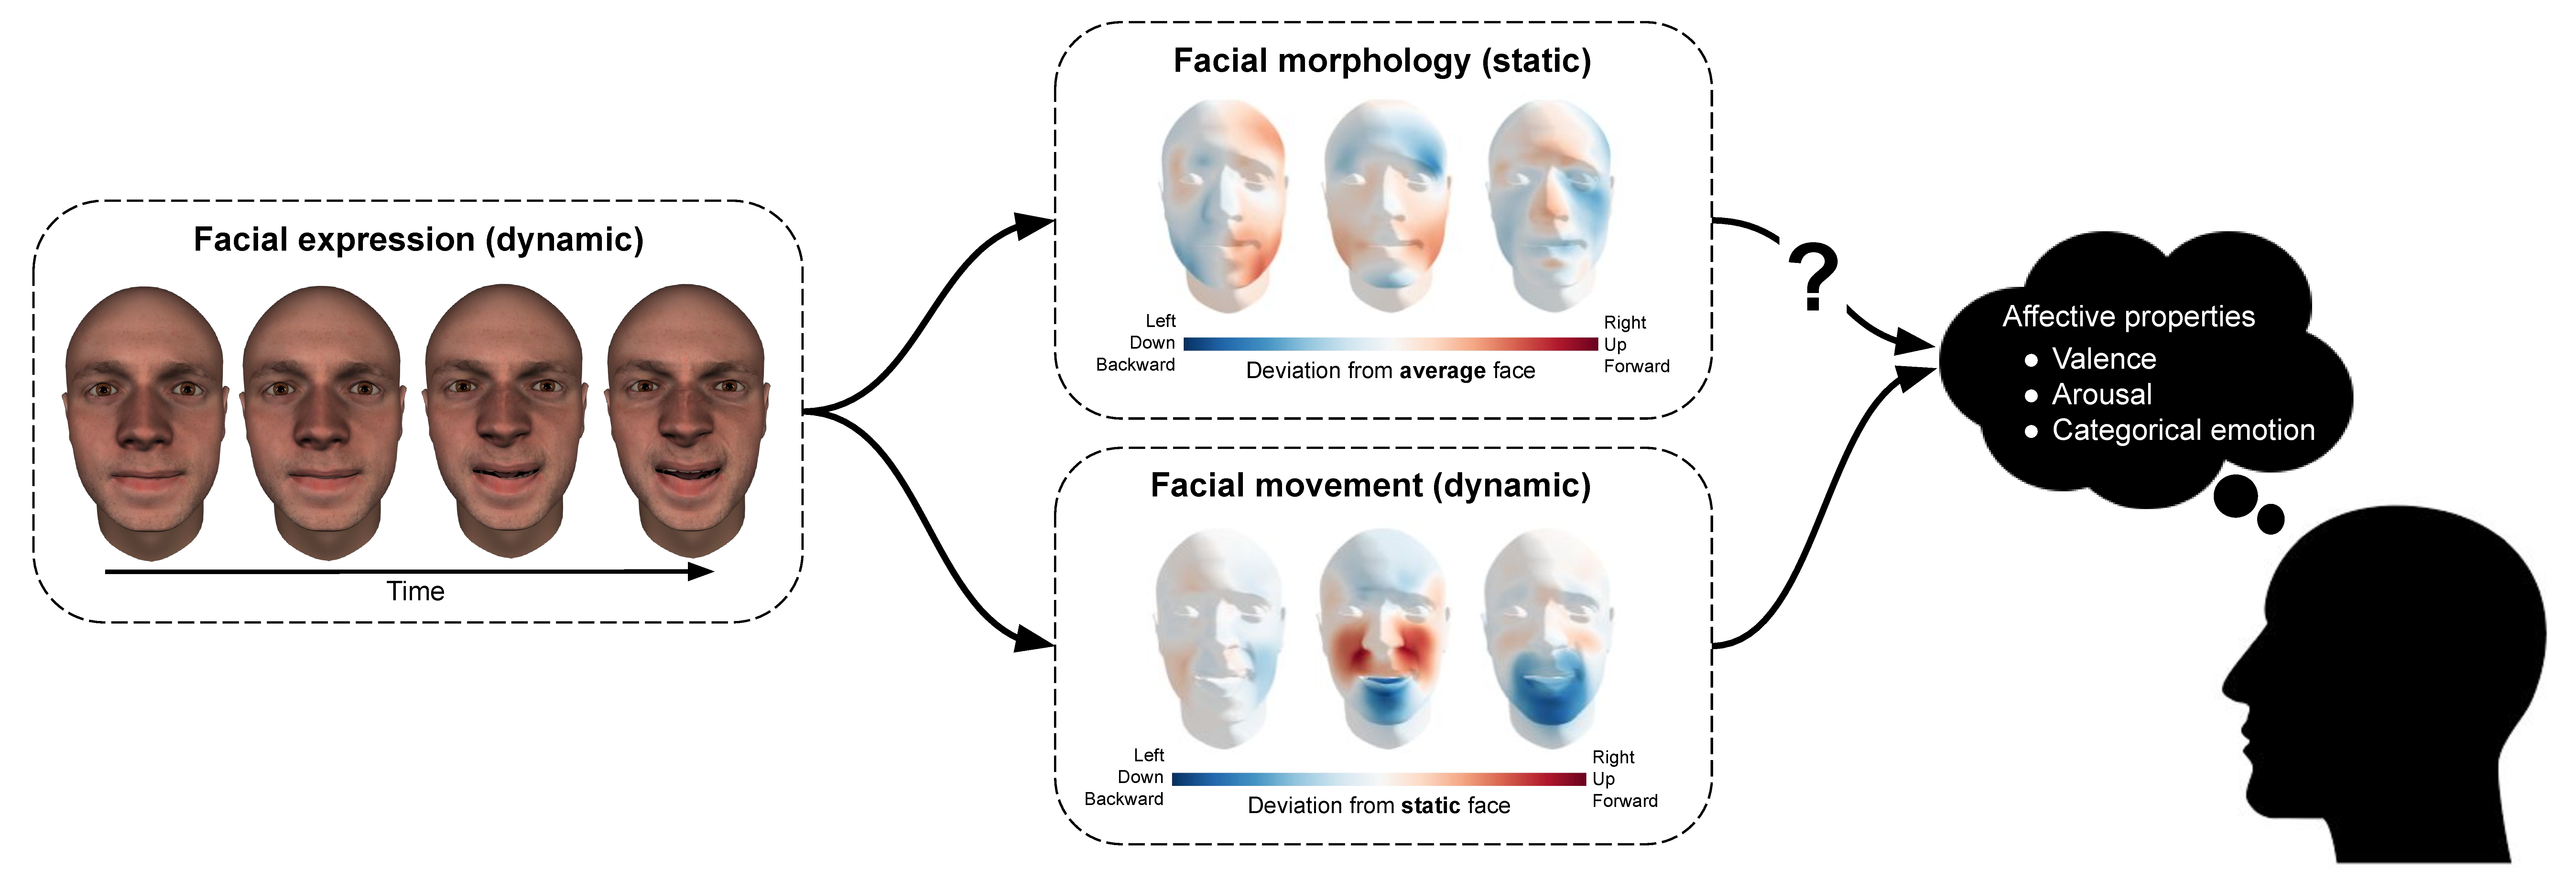
\includegraphics{_bookdown_files/static-vs-dynamic-files/figures/figure_1.pdf}
\caption{\label{fig:fig-svsd-1}Decomposition of facial expressions in static information (facial morphology) and dynamic information (facial movement), where static information is operationalized as shape deviation relative to the average face while dynamic information is operationalized as shape deviation relative to the static face. The current study's aim is to quantify the importance of static information, relative to dynamic information, in affective perception.}
\end{figure}



\hypertarget{svsd-methods}{%
\section{Methods}\label{svsd-methods}}

\hypertarget{svsd-participants}{%
\subsection{Participants}\label{svsd-participants}}

Thirteen participants (7 female, 6 male) participated in the ``Facial Expression Encoding and Decoding'' project, which consisted of six psychophysics sessions and six (7T) MRI sessions. Participants were recruited through Facebook. With the exception of three participants, all participants were students of the Research Master Psychology or master Brain \& Cognitive Sciences at the University of Amsterdam. Several strict exclusion criteria for participation were applied, including standard MRI safety-related exclusion criteria, psychiatric conditions, use of psychopharmacological medication, color blindness, and difficulty with remembering faces. Additionally, participants had to have participated in MRI research before and had to be between 18 and 30 years of age (resulting sample \emph{M}\textsubscript{age} = 22.6, \emph{SD}\textsubscript{age} = 3.7).

Across six psychophysics sessions, participants rated the perceived valence, arousal, and categorical emotion of short clips of dynamic facial expressions. These stimuli were generated using a 3D Morphable Modeling toolbox developed by and described in Yu et al. (\protect\hyperlink{ref-Yu2012-ag}{2012}). The toolbox allows to generate short video clips of facial expressions with a configuration of prespecified ``action units'' (AUs) that describe particular visually recognizable facial movements. It does so by manipulating the structure of a 3D mesh representing the surface of the face according to the expected deformation in response to the activation of one or more AUs. Apart from amplitude (ranging from 0, inactive, to 1, maximally activated), several temporal parameters corresponding to the AU activation (onset latency, offset latency, acceleration, deceleration, and peak latency) can be manipulated. In the toolbox, AU animations can be applied to any 3D face mesh from a database of 487 different faces (``face identities''), which vary in sex, age, and ethnicity.

For our stimuli, we used 50 different face identities that were restricted to be of Western-Caucasian ethnicity and to an age between 18 and 30 years old (i.e., the same age range as our participants). This set of face identities contained 36 female faces and 14 male faces. To animate each face stimulus, we selected a random subset of AUs from a set of twenty bilateral AUs (AU1, AU2, AU4, AU5, AU6, AU7, AU9, AU10Open, AU11, AU12, AU13, AU14, AU15, AU16Open, AU17, AU20, AU24, AU25, AU27i, AU43). The number of AUs for each stimulus were drawn randomly from a binomial distribution with parameters n = 6 and p = 0.5 (but with a minimum of 1 AU). The amplitude of each AU activation was randomly selected from three equidistant values (0.333, 0.667, and 1). The temporal parameters were the same for each stimulus, which corresponds to a stimulus with a duration of 1.25 seconds and in which each AU activation peaks at 0.7 seconds. Each of the 3D face meshes belonging to a single dynamic stimulus was rendered as a short (2D) video clip with a resolution of 600 × 800 pixels containing 30 frames and a frame rate of 24 frames per second.

\hypertarget{svsd-experimental-design}{%
\subsection{Experimental design}\label{svsd-experimental-design}}

In total, 752 unique AU configurations were generated with the parameters described above. This process was done separately for two disjoint sets of AU configurations: one set of 696 configurations functioning as the \emph{optimization set} (used for model fitting) and one set of 56 configurations functioning as the \emph{test set} (used for model validation; see \protect\hyperlink{svsd-cv}{Cross-validation} section). To minimize correlation between AU variables, the sampling process of the number of AUs and AU amplitudes was iterated 10,000 times and the selection yielding the smallest absolute maximum correlation across all AU pairs was chosen (final \(r = 0.093\)). Then, the AU configurations were randomly allocated to the 50 face identities. To minimize the correlation between face identity and AUs, this random allocation was iterated 10,000 times and the selection yielding the smallest (absolute) maximum correlation across all AU-face identity pairs (final \(r = 0.126\)) was chosen. This counterbalancing process was done separately for the optimization and test set.

\hypertarget{svsd-procedure}{%
\subsection{Procedure}\label{svsd-procedure}}

Each participant completed five psychophysics sessions in which they rated a subset of the facial expression stimuli. In the sixth session, participants rated the 50 static faces (i.e., without AU animations) on their perceived attractiveness, dominance, trustworthiness, valence and arousal. These ratings are not used in the current study. Because the test set trials were repeated three times (to estimate a noise ceiling; see Noise ceiling estimation section), the total number of rated stimuli was (696 + 56 × 3 = ) 864. Originally, three sessions were planned in which participants rated 288 stimuli each. Due to a programming bug, however, all but one of the participants rated (unbeknownst to them) the same 288 stimuli in these three sessions. As such, participants completed two extra sessions in which they rated the remaining stimuli with the exception of the (56 × 2 =) 112 test trials, because the three repetitions needed to estimate the noise ceiling were already obtained in the first three sessions. As such, the total number of stimulus ratings was (288 × 3 + 232 × 2 = ) 1328 (and 864 ratings for the single participant without the accidental session repeats).

In each session, the 288 stimuli (or 232 stimuli in session 4 and 5) were rated on three affective properties: categorical emotion, valence, and arousal. Categorical emotion and valence/arousal were rated on separate trials, so each of the stimuli were presented twice (once for a categorical emotion rating and once for a valence/arousal rating). Stimuli were presented in blocks of 36 trials, in which either categorical emotion or valence/arousal was rated. The trial block's rating type was chosen randomly.

Each session lasted approximately 1.5 hours, which included breaks (after each rating block), setting up and calibrating the eyetracker (which is not used in the current study), an extensive instruction, and a set of practice trials (only in the first block of each session; 10 categorical emotions and 10 valence/arousal ratings). Participants completed the ratings in a dimly lit room, with their head resting on a chin rest (to minimize head movement for the concurrent eyetracking), positioned 80 centimeters from a full HD (1920 × 1080 pixels) monitor (51 × 28.50 cm) on which the rating task was presented using the software package PsychoPy2 (v1.84; Peirce et al., \protect\hyperlink{ref-Peirce2019-rj}{2019}). Participants used a standard mouse (used with their dominant hand) to submit responses during the rating task.

\hypertarget{svsd-stimulus-presentation}{%
\subsubsection{Stimulus presentation}\label{svsd-stimulus-presentation}}

Stimuli were presented on a gray background (RGB: 94, 94, 94). Each trial block started with a cue regarding the affective property that should be rated (categorical emotion or valence/arousal) and was followed by a ten second baseline period presenting a fixation target (a white circle with a diameter of 0.3 degrees visual degree, DVA). Then, each facial expression stimulus was presented for 1.25 seconds (the full duration of the clip). The stimulus was shown at the center of the monitor with a size of 6 × 8 DVA (preserving the aspect ratio of the original clip, i.e., 600 × 800 pixels). The stimulus was followed by an interval of 1 second plus a duration drawn from an exponential distribution (with λ = 1) in which only the fixation target was shown. This interval was followed by the presentation of the rating screen (discussed below). The rating screen was shown until the participant gave a response (mouse click). Another interval followed (which included a fixation target) with a duration of 1 second plus a duration drawn from an exponential distribution (with \(\lambda = 1\)), after which the next stimulus was shown. After all 36 trials of a trial block, another baseline period including a fixation target was shown and was followed by the rating type cue of the next block, which the participant could start by a mouse click. After four trial blocks, participants could take a break if desired.

\hypertarget{categorical-emotion-ratings}{%
\subsubsection{Categorical emotion ratings}\label{categorical-emotion-ratings}}

For the categorical emotion ratings, participants were instructed to ``Judge the faces with regards to the emotion that the face shows, if any'' (in Dutch: ``Beoordeel de gezichten op de emotie die de gezichten (mogelijk) laten zien''). For each categorical emotion rating, participants were presented with a prompt which included six trapezoids (with the corresponding labels ``anger'', ``disgust'', ``fear'', ``happiness'', ``sadness'', and ``surprise'' next to it) and a single circle (with the label ``None'') arranged in a circle with equal angles between each of the seven options (i.e., 360/7 degrees; see Figure \ref{fig:fig-svsd-2}). The trapezoids had a length of 7 DVA, the circle had a radius of 1 DVA, and the text labels had a text height of 0.7 DVA; the trapezoids, circle, and text were all white. At the onset of the rating prompt, the mouse cursor appeared in the middle of the screen. Participants were instructed to click on the trapezoid corresponding to the perceived emotion from the previously shown facial expression stimulus. Furthermore, participants were instructed to simultaneously rate the intensity of the emotion, which was linked to the radial position of the mouse click within the trapezoid, where responses closer to the center indicated lower intensity and responses farther away from the center indicated higher intensity. After the participant clicked on the trapezoid, the trapezoid changed color from white to black anywhere between the response and the side of the trapezoid closest to the center (see Figure 2). Whenever the facial expression stimulus did not match any of the six categorical emotion labels (``anger'', ``disgust'', ``fear'', ``happiness'', ``sadness'', and ``surprise''), participants were instructed to click on the circle above the label ``None'' (``Geen van allen'' in Dutch). There was no intensity rating associated with ``None'' responses. After a response and the change in color of the selected trapezoid or circle, the rating prompt remained on screen for 0.2 seconds. There was no response time limit for the ratings.

\hypertarget{valencearousal-ratings}{%
\subsubsection{Valence/arousal ratings}\label{valencearousal-ratings}}

For the valence and arousal ratings, participants were asked to rate how they experienced each face in terms of arousal (on a scale ranging from ``not activated'' to ``activated'') and valence (on a scale ranging from ``unpleasant'' to ``pleasant''). The instructions explained the valence dimension as follows: ``On the pleasant/unpleasant dimension, you should indicate how \emph{you} experience the faces'' (in Dutch: ``Met de onprettig/prettig dimensie geef je aan hoe \emph{jij} de gezichten ervaart''). The instructions explained the arousal dimension as follows: ``On the not activated/activated dimension, you indicate how much the face activates you. With `activated', we mean that the face makes you feel alert, energized, and/or tense. With `not activated', we mean that the face makes you feel calm, quiet, and/or relaxed'' (in Dutch: ``Met de niet geactiveerd/geactiveerd dimensie geef je aan in hoeverre het gezicht jou activeert. Met ``geactiveerd'' bedoelen we dat het gezicht je alert, energiek, en/of gespannen doet voelen; met ``niet geactiveerd'' bedoelen we dat het gezicht je kalm, rustig, en/of ontspannen doet voelen'').

Valence and arousal ratings were acquired using a single rating prompt (see Figure \ref{fig:fig-svsd-2}). This prompt included two axes (white lines), a horizontal and a vertical one, of equal length (14 DVA). The horizontal axis represented the arousal axis with negative values indicating low arousal (``Not activated'', or ``Niet geactiveerd'' in Dutch) and positive values indicating high arousal (``Activated'', or ``Geactiveerd'' in Dutch). The vertical axis represented the valence axis with positive values indicating positive valence (``Pleasant'', or ``Prettig'' in Dutch) and negative values indicating negative valence (``Unpleasant'', or ``Onprettig'' in Dutch). Labels at the ends of the axis lines were white and had a text height of 0.7 DVA. Participants were instructed to indicate the valence and arousal of the previously shown facial expression facial expression stimulus by a single mouse click anywhere within the 2D space. After a response, a white circle (0.3 DVA) appeared at the clicked position for 0.2 seconds, after which the rating prompt disappeared.

\begin{figure}
\centering
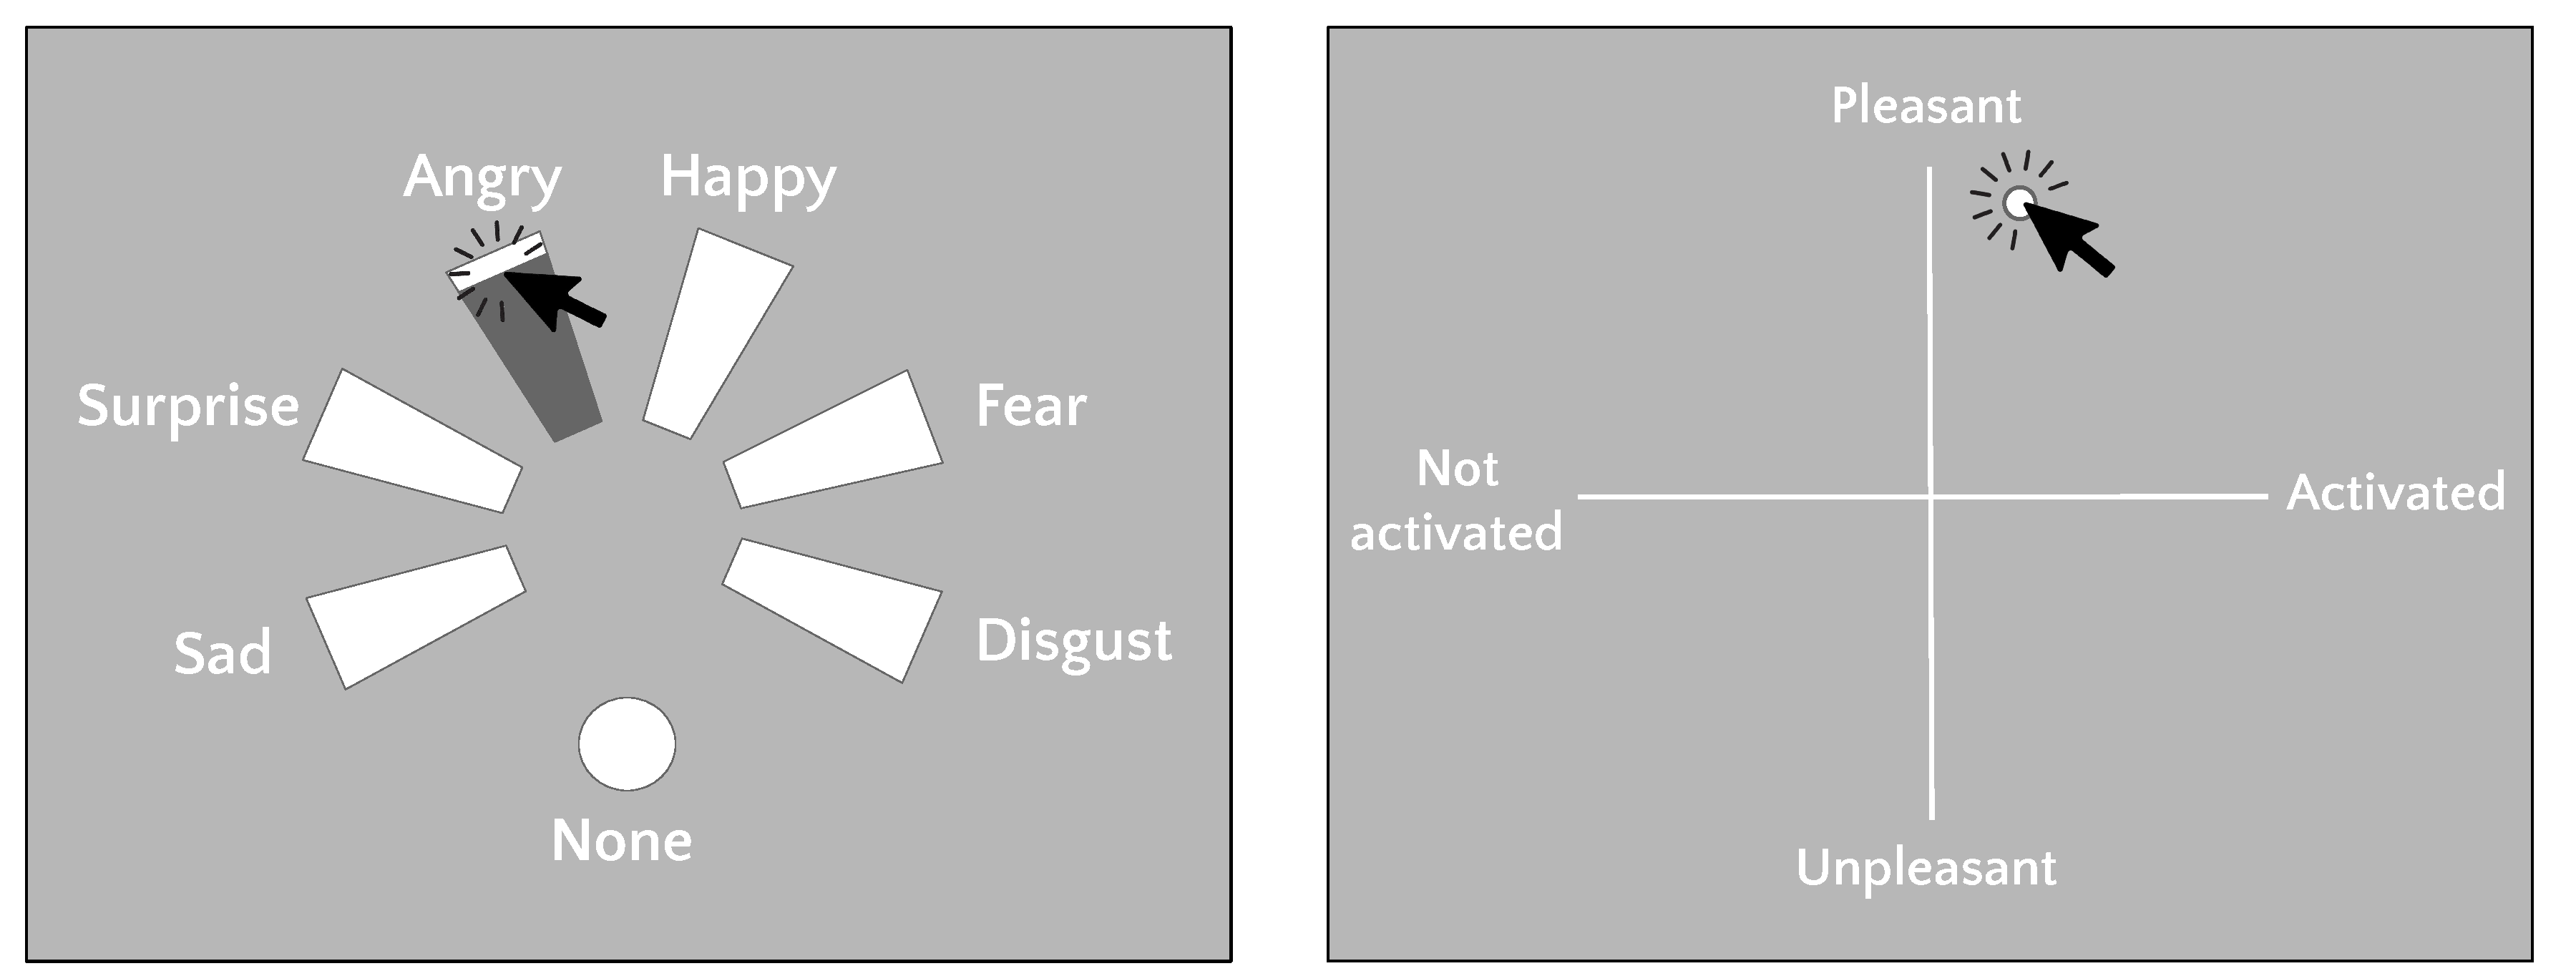
\includegraphics{_bookdown_files/static-vs-dynamic-files/figures/figure_2.pdf}
\caption{\label{fig:fig-svsd-2}Prompts for categorical emotion ratings (left) and valence/arousal ratings (right).}
\end{figure}



\hypertarget{svsd-data-preproc}{%
\subsection{Data preprocessing}\label{svsd-data-preproc}}

\hypertarget{rating-preprocessing}{%
\subsubsection{Rating preprocessing}\label{rating-preprocessing}}

For the categorical emotion analyses, we removed all ratings in which the participant responded with ``None''. This left on average 1125 trials (\emph{SD} = 165), which is 87\% of the total number of trials. The valence and arousal ratings were not filtered or otherwise preprocessed. The accidentally repeated trials from session 1 (that do not belong to the test set; see \protect\hyperlink{svsd-cv}{Cross-validation} section) were reduced to a single rating for each unique stimulus by taking the most frequent emotion label (for the categorical emotion ratings) or the average rating value (for the valence/arousal ratings) across repetitions. In addition, the valence and arousal ratings were mean-centered separately for the optimization and test set to correct for spurious differences in the mean across the two partitions.

\hypertarget{static-and-dynamic-feature-operationalization}{%
\subsubsection{Static and dynamic feature operationalization}\label{static-and-dynamic-feature-operationalization}}

As an operationalization of face structure, we use the set of 3D face meshes underlying each dynamic facial expression stimulus. The reason for focusing on the underlying 3D face mesh, instead of the rendered 2D pixel array actually shown to the participants, is that the 3D face mesh allows to isolate face structure information from face texture information while in the 2D pixel space these two factors are confounded. In the 3D face space, each stimulus can be represented as a collection of 30 meshes (corresponding to the 30 frames in each animation), each containing a set of 3D coordinates making up the \emph{vertices} of the mesh. In our stimulus set, each 3D face mesh has 31049 vertices. As such, any given stimulus can be represented as a 30 (frames) × (vertices) × 3 (coordinates) array with values that represent the position of the vertices in real-world space.

The first step in our feature operationalization pipeline is to separate the static and dynamic information. We operationalize the static information as the 3D face mesh corresponding to the first frame of each stimulus (which corresponds to a ``static'' or ``neutral'' face mesh without any AU activation). Using this operationalization, the static information from two stimuli with different AUs (but the same face identity) is equivalent. We operationalize the dynamic information for each stimulus as the \emph{difference} between the vertex positions at the frame containing the peak AU activation (frame 15) and the first frame. As such, both the static information and the dynamic information of each stimulus can be represented as a 31049 (vertices) × 3 (coordinates) array.

Using all vertex positions as features means that the number of features (i.e., 31049 × 3 = 93147) would vastly outnumber the number of observations (i.e., 752 unique dynamic facial expressions), which makes model fitting prohibitively computationally expensive and bears a high risk of overfitting. As such, reducing the number of features is desirable. The fact that the vertices are highly spatially correlated (i.e., neighboring vertices likely have similar coordinates) warrants using principal component analysis (PCA) to reduce the total feature space. Here, we use PCA to reduce the original feature space (containing 93147 dimensions) to a 50-dimensional space containing variables that represent linear combinations of the original features. Formally, the PCA model estimates a 2D weight matrix, \(W\), with dimensions 50 × 93147 and a mean vector, \(\hat{\mu}\), with length 93147, which are then used to transform the original set of vertices (\(V\); flattened across coordinates) into a 50-dimensional set of features (\(X\)):

\begin{equation}
X = (V - \hat{\mu})\hat{W}^{T}
\end{equation}

In this lower-dimensional feature space, almost all variance from the high-dimensional feature space is preserved: about 99.99\% for the static feature space and about 99.95\% of the dynamic feature space (see Supplementary Figure \ref{fig:fig-svsd-S1}). The representation of the top four PCA components in vertex space are, for both the static and dynamic feature set separately, visualized in Figure \ref{fig:fig-svsd-3}, which shows that each PCA component represents an interpretable facial movement (e.g., PC1 of the dynamic feature set represents a mouth drop and PC1 of the static feature set represents a relatively wide and long face with a relatively strongly protruding nose and brow).

\begin{figure}
\centering
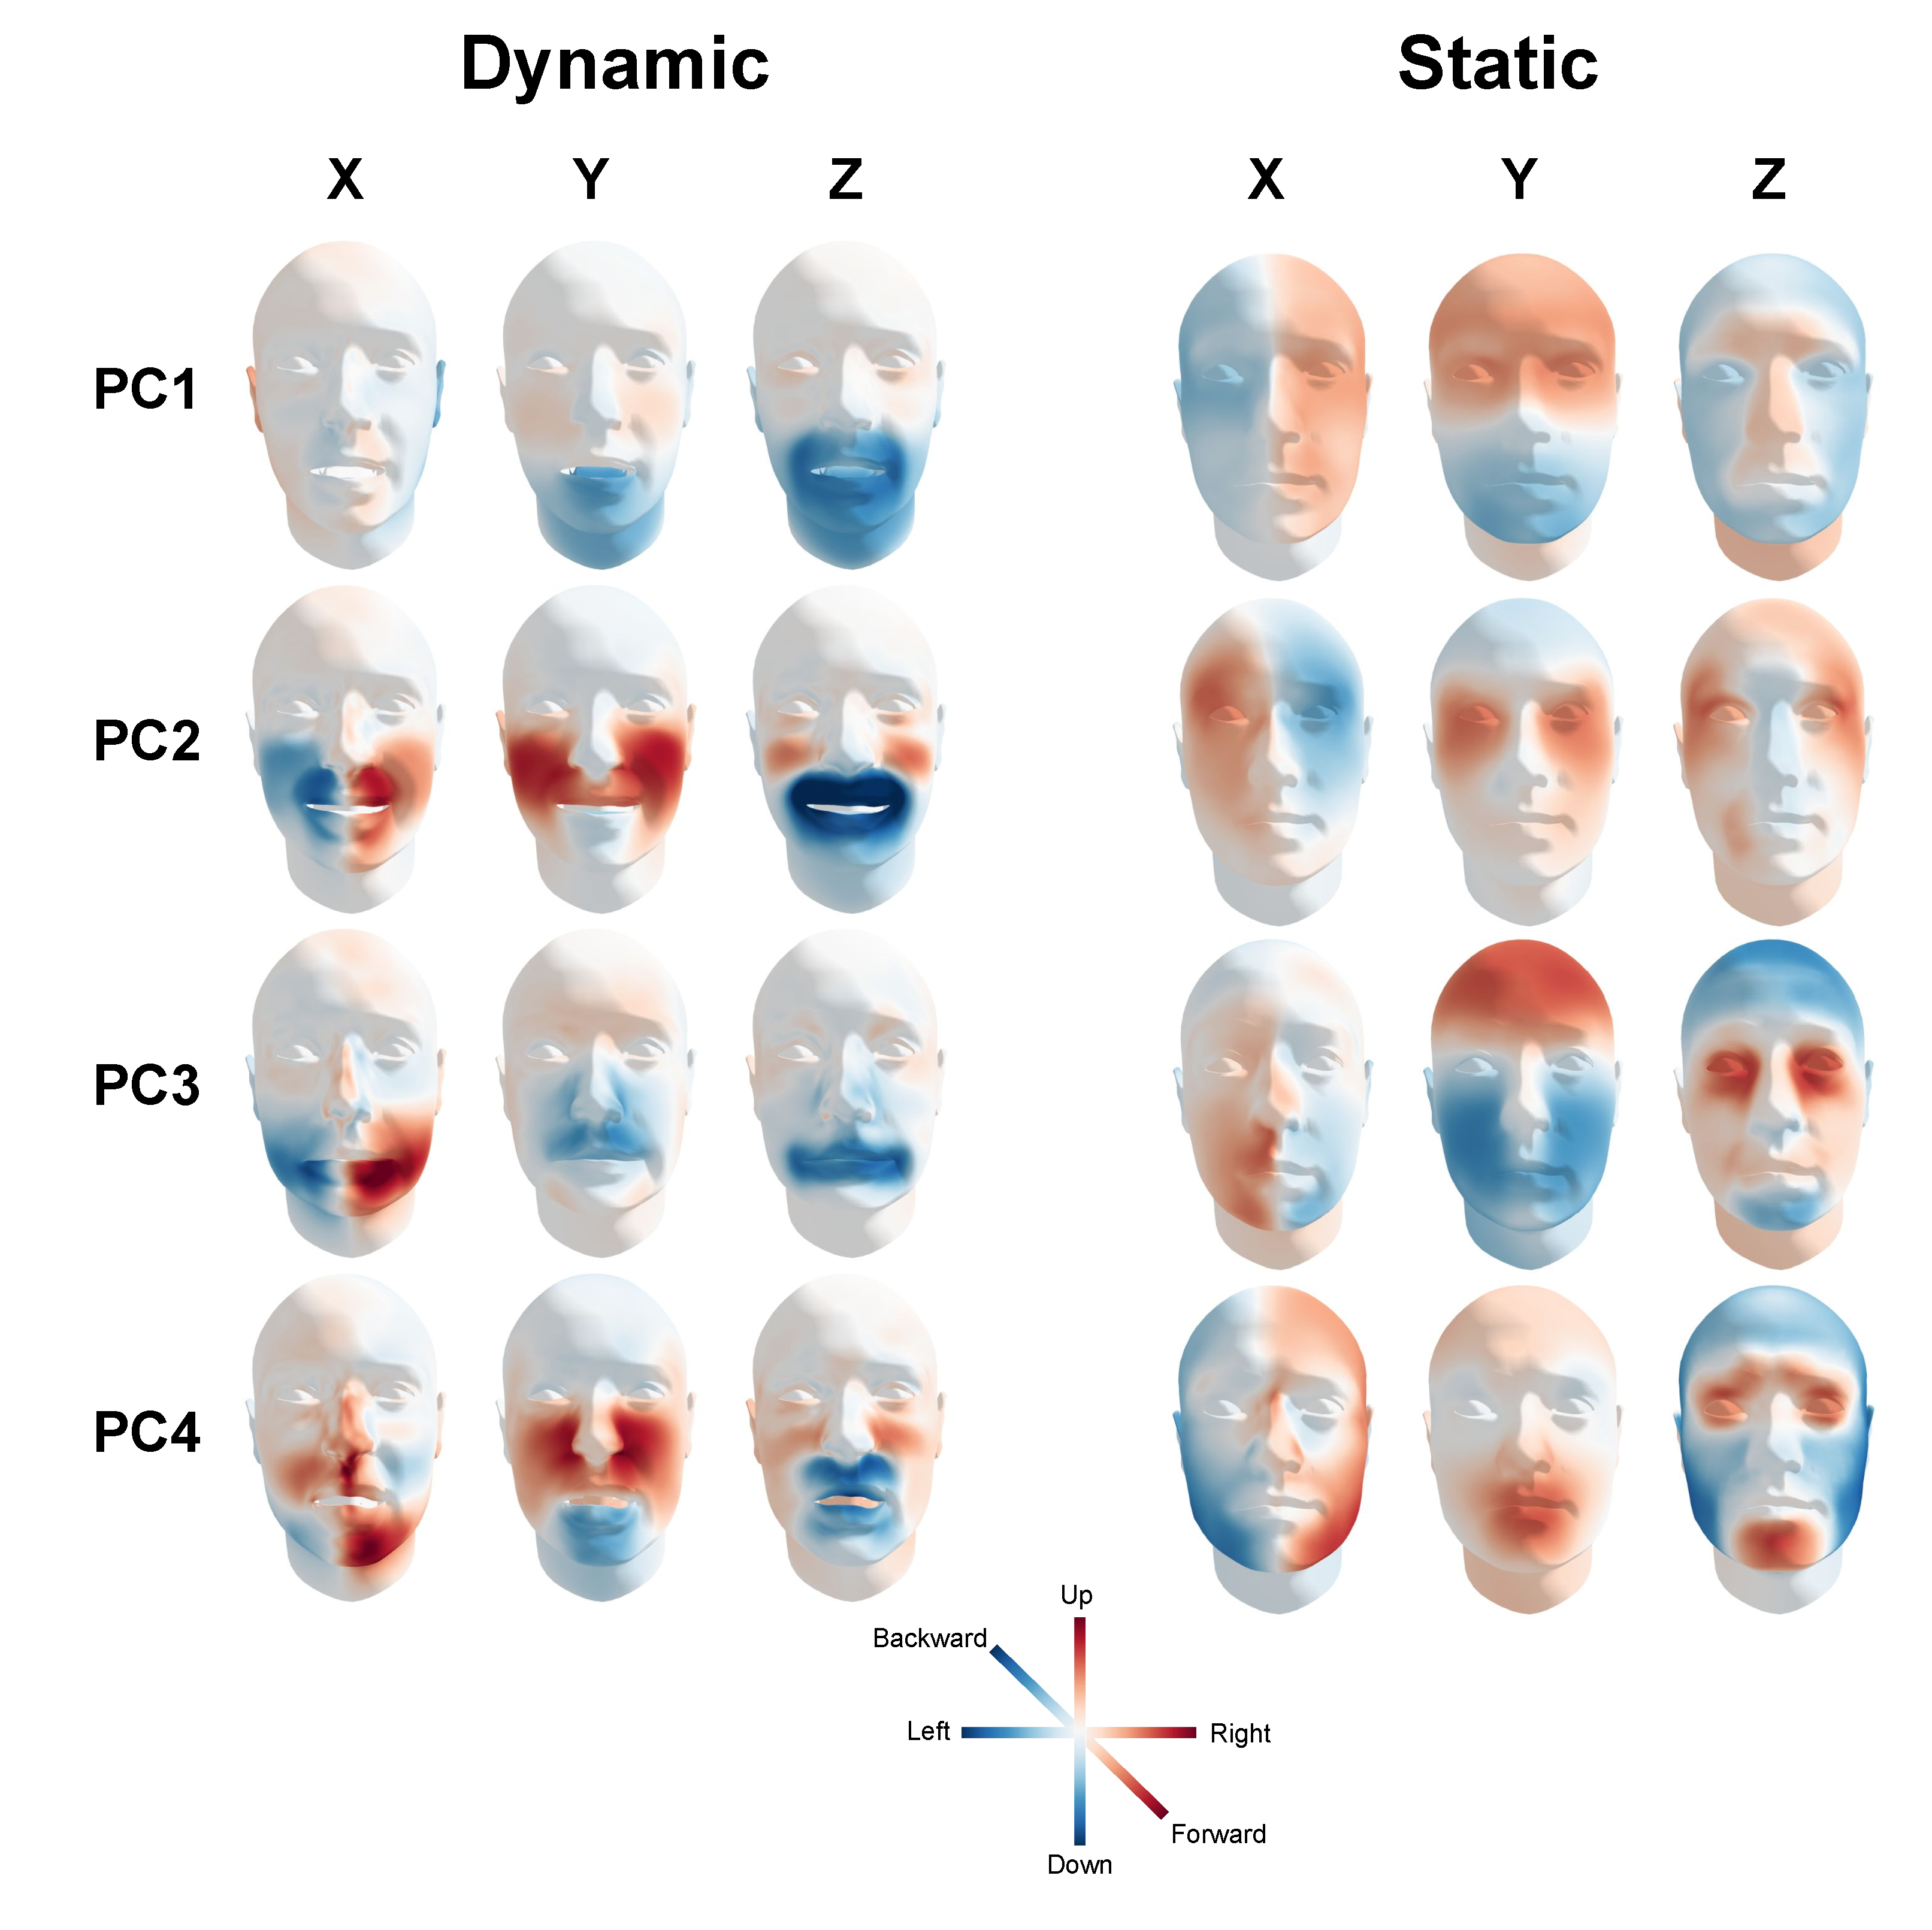
\includegraphics{_bookdown_files/static-vs-dynamic-files/figures/figure_3.pdf}
\caption{\label{fig:fig-svsd-3}Visualization of the extracted PCA components. The first four PCA components of both the dynamic features (left) and static features (right) are visualized by plotting the inverse transform of a single low-dimensional feature set to 3 standard deviations above the average (\(X_{j} := 3\hat{\sigma}_{X_{j}}\)). Colors represent the signed deviation from the mean in standard deviations.}
\end{figure}



Finally, both the static and dynamic PCA-transformed features (\(X_{j}\)) are divided by their estimated standard deviation (\(\hat{\sigma}_{j}\)) across observations:

\begin{equation}
X_{j} := \frac{X_{j}}{\hat{\sigma}_{j}}
\end{equation}

This operation makes sure that each feature has the same scale and thus each feature is equally strongly regularized during model fitting (see \protect\hyperlink{svsd-pred-analysis}{Predictive analysis} section). Note that usually each feature is additionally mean-centered as well, but this is not necessary because the PCA transform already centers the data.

In the current article, we will refer to a set of PCA-transformed features (\(X\)) as a \emph{feature set}. In addition to having a dynamic and static feature set, we also horizontally concatenated these two feature sets to create a combined feature set (which thus contains 100 features), which serves to investigate to what extent the two feature sets explain unique variance in the target variables.

\hypertarget{svsd-pred-analysis}{%
\subsection{Predictive analysis}\label{svsd-pred-analysis}}

For our main analysis, we predicted the categorical emotion, valence, and arousal ratings based on static and dynamic features using separate models for each participant. Because the categorical emotion ratings represent a categorical variable, the categorical emotion analysis used a classification model. The valence and arousal ratings represent continuous variables and are therefore analyzed using a regression model. These two types of models are discussed in turn.

\hypertarget{svsd-cat-emo}{%
\subsubsection{Categorical emotion model}\label{svsd-cat-emo}}

The categorical emotion analysis used a regularized multinomial logistic regression model as implemented in the Python package \emph{scikit-learn} (Pedregosa et al., \protect\hyperlink{ref-pedregosa2011scikit}{2011}). The choice for this particular predictive model stems from its probabilistic formulation, which makes it suitable for the Bayesian model inversion procedure described in the \protect\hyperlink{svsd-bayes}{Bayesian reconstruction} section. Formally, the multinomial logistic regression model assumes that the target variable is distributed according to a categorical distribution parameterized as follows:

\begin{equation}
p(y) \sim \mathrm{Categorical}(g(X\beta + \alpha))
\end{equation}

where \(\beta\) represents a set of parameters that are linearly combined with the feature values (\(X\)) and an intercept term (\(\alpha\)), which is passed through the softmax function, \(g\):

\begin{equation}
g(X_{i}\beta + \alpha) = \frac{e^{X_{ij}\beta + \alpha}}{\sum_{j=1}^{P}e^{X_{ij}\beta + \alpha}}
\end{equation}

where \(p(y_{i} | X_{i})\) is a vector with a length equal to the number of classes. Although it is possible to derive discrete predictions by subsequently taking the argmax across the vector with class probabilities, we only use the probabilistic predictions because we use a probabilistic model performance metric (Tjur's pseudo \(R^{2}\); see \protect\hyperlink{svsd-perf}{Performance metrics} section). In the context of our categorical emotion analysis, the fitted multinomial logistic regression model outputs predictions in the format of the probability of each of the six categorical emotions given the set of static or dynamic (or their combination) features of a given facial expression stimulus. The logistic regression model was used with balanced class weights to avoid effects due to imbalance across class frequencies, a regularization parameter (C) of 10, and a liblinear solver.

\hypertarget{svsd-valaro}{%
\subsubsection{Valence and arousal models}\label{svsd-valaro}}

Both the valence and arousal analysis used a ridge regression model as implemented in the Python package \emph{scikit-learn}. Like the multinomial logistic regression model, linear regression models (including the ridge regression model) have a well-defined probabilistic formulation, which assumes that the target variable (\(y_{i}\)) is normally distributed:

\begin{equation}
p(y) = \mathcal{N}(X\beta, \sigma_{\epsilon}I)
\end{equation}

where \(~X\beta\) represents the mean and \(\sigma_{\epsilon}I\) the standard deviation of the normal distribution. Note that we do not estimate an intercept term (\(\alpha\)) because we standardize our features (\(X\)) and target variable (\(y\)) before the analysis. After estimating the parameters \(\beta\) and \(\sigma_{\epsilon}\) (i.e., \(\hat{\beta}\) and \(\hat{\sigma}_{\epsilon}\)), predictions for a given observation (\(X_{i}\)) can be made as follows:

\begin{equation}
\hat{y}_{i} = X_{i}\hat{\beta}
\end{equation}

In the context of our valence and arousal model, this means that the valence and arousal values are predicted on the basis of a linear combination of the static or dynamic features. The ridge regression model was fitted with a regularization parameter of 500 and without an intercept.

\hypertarget{svsd-cv}{%
\subsubsection{Cross-validation procedure}\label{svsd-cv}}

To facilitate optimization of the analysis and model hyperparameters without the risk of overfitting (Kriegeskorte et al., \protect\hyperlink{ref-kriegeskorte2009circular}{2009}), the data (i.e., all 752 unique stimuli and associated ratings) were divided into two independent sets: an optimization set with 564 unique stimuli and a test set with 150 unique stimuli (which contains 450 ratings, because each test trial was repeated three times in order to estimate a within-participant noise ceiling). Note that the set of unique test set stimuli is composed of the 56 stimuli originally designated as test set stimuli and an additional 96 stimuli randomly sampled from the accidental repeated trials from the first session; the reason to increase the test set size is to reduce the variance in the estimate of model performance (Varoquaux et al., \protect\hyperlink{ref-Varoquaux2017-fj}{2017}; Varoquaux, \protect\hyperlink{ref-Varoquaux2018-uo}{2018}). The distribution of categorical emotion, valence, and arousal ratings is visualized, separately for the optimization and test set, in Supplementary Figure \ref{fig:fig-svsd-S2}, which shows that the two sets are very similar in their rating distributions.

Within the optimization set, we compared different preprocessing techniques (such as standardization before or after PCA fitting) and model hyperparameters (such as the model's regularization parameter, which was evaluated for \(\alpha\) and \(\frac{1}{C}\): 0.01, 0.1, 1, 10, 50, 100, 500, 1000). This was done using repeated 10-fold cross-validation within the optimization set, which entails fitting the model on 90\% of the data (the ``train set'') and evaluating the model performance on the prediction of the left out 10\% of the data (the ``validation set''). The results of this optimization procedure indicated that a regularization parameter of 10 for the logistic regression model and a regularization parameter of 500 for the regression models led to the highest cross-validated model performance within the optimization set, which were used for each participant-specific model.

This cross-validation procedure within the optimization set was repeated multiple times to optimize the preprocessing and model hyperparameters, which results in a positively biased estimate of cross-validated model performance (Kriegeskorte et al., \protect\hyperlink{ref-kriegeskorte2009circular}{2009}). As such, we fitted each model with the optimal hyperparameters (as reported in the \protect\hyperlink{svsd-cat-emo}{Categorical emotion model} and \protect\hyperlink{svsd-valaro}{Valence/arousal models} sections) once more on the entire optimization set and subsequently cross-validated it to the test set. This cross-validation from the optimization to test set was only done once to ensure an unbiased estimate of cross-validated model performance. Notably, in the test set, the trial repetitions were not reduced to a single rating in order to estimate the noise ceiling specifically for the model performance on the test set.

\hypertarget{svsd-perf}{%
\subsubsection{Performance metrics}\label{svsd-perf}}

To evaluate the cross-validated model performance of the categorical emotion model, we used Tjur's pseudo \(R^{2}\) score (Tjur, \protect\hyperlink{ref-Tjur2009-dp}{2009}). We chose this particular metric instead of more well-known metrics for classification models (such as accuracy) because it is insensitive to class frequency, allows for class-specific scores, and has the same scale and interpretation as the \(R^{2}\) score commonly used for regression models (Dinga et al., \protect\hyperlink{ref-Dinga2020-si}{2020}). To evaluate the cross-validated model performance of the valence and arousal models, we used the \(R^{2}\) score. Note that the theoretical maximum value of both Tjur's pseudo \(R^{2}\) score and the regular \(R^{2}\) score is 1, while the minimum of Tjur's pseudo \(R^{2}\) score is -1 and the minimum for the regular \(R^{2}\) score is unbounded; chance level for both metrics is 0.

\hypertarget{population-prevalence}{%
\subsubsection{Population prevalence}\label{population-prevalence}}

Although participant-specific cross-validated model performance scores are unbiased estimates of generalizability, above chance level estimates may be due to chance (although this is unlikely given the relatively large size of our test set; Varoquaux, \protect\hyperlink{ref-Varoquaux2018-uo}{2018}). Additionally, reporting only summary statistics (such as the mean or median) of the set of within-participant model performance estimates ignores the between-participant variance. One possibility to summarize and quantify model performance across the set of participants is to test their mean score against the theoretical chance level using a one-sample \emph{t}-test. This approach, however, is invalid for unsigned metrics, such as the (pseudo) \(R^{2}\) scores used in this study, which logically cannot have a population mean below chance level and thus cannot be tested using a one-sample \emph{t}-test (which assumes a symmetric gaussian sampling distribution around the chance level; Allefeld et al., \protect\hyperlink{ref-Allefeld2016-xp}{2016}).

An alternative statistical framework is provided by \emph{prevalence inference} (Allefeld et al., \protect\hyperlink{ref-Allefeld2016-xp}{2016}; Rosenblatt et al., \protect\hyperlink{ref-Rosenblatt2014-az}{2014}), which estimates the proportion of the population that would show the effect of interest. Here, we use the Bayesian approach to prevalence inference described by Ince et al. (\protect\hyperlink{ref-Ince2020-mr}{2020}). This particular implementation estimates a posterior distribution of the population prevalence proportion (a number between 0 and 1), which is based on the number of statistically significant effects across participants. Statistical significance for a given participant (i.e., the ``first-level test statistic'') is computed using a non-parametric permutation test (Allefeld et al., \protect\hyperlink{ref-Allefeld2016-xp}{2016}; Ojala \& Garriga, \protect\hyperlink{ref-Ojala2010-rc}{2010}), in which the observed cross-validated model performance score is compared to the distribution of model performance scores resulting from the model predictions on permuted test set values. Formally, the \emph{p}-value corresponding to an observed score, \(sc^{\mathrm{obs}}\), given a set of \emph{Q} permutation values, \(sc^{\mathrm{perm}}\), is computed as follows:

\begin{equation}
p = \frac{\sum_{p=1}^{Q} I(sc_{i}^{\mathrm{perm}} \geq sc^{\mathrm{obs}}) + 1}{Q + 1}
\end{equation}

where \(I\) is an indicator function return 1 when the expression in brackets \((sc_{i}^{\mathrm{perm}} \geq sc^{\mathrm{obs}})\) is true and 0 otherwise. In our analyses, we ran 1000 permutations and used a significance level (\(\alpha\)) of 0.05. Note that although significance of participant-specific effects is computed using a binary decision threshold (as is done in traditional null-hypothesis significance testing), the posterior resulting from the Bayesian prevalence inference analysis is not thresholded.

The issues associated with group-level tests of model performance against chance level do not apply to group-level tests between model performance estimates of different classes of the target variable (e.g., between different emotions), because a symmetric distribution can be assumed for these values.

\hypertarget{noise-ceiling-estimation}{%
\subsection{Noise ceiling estimation}\label{noise-ceiling-estimation}}

If there is measurement noise in the target variable, perfect model performance (i.e., at the theoretical maximum) is impossible. In case of measurement noise, it is more insightful to compare model performance to an estimate of the \emph{noise ceiling}, an upper bound that is adjusted for measurement noise in the target variable (Lage-Castellanos et al., \protect\hyperlink{ref-lage2019methods}{2019}). We developed a method to derive noise ceilings for classification models, which is reported and explained in detail in Chapter 7. We use this method to estimate noise ceilings for our categorical emotion models.

For the valence and arousal models, we developed a method to estimate a noise ceiling, assuming that the regular \(R^{2}\) score is used, that is very similar to the aforementioned method to estimate noise ceilings for classification models (see for a related method, Sahani \& Linden, \protect\hyperlink{ref-Sahani2003-kk}{2003}; Schoppe et al., \protect\hyperlink{ref-Schoppe2016-bu}{2016}). Recall that the \(R^{2}\) score is computed as 1 minus the ratio of the residual sum of squares (RSS) to the total sums of squares (TSS):

\begin{equation}
R^{2} = 1 - \frac{RSS}{TSS} = 1 - \frac{\sum_{i = 1}^{n}(y_{i} - \hat{y}_{i})^{2}}{\sum_{i = 1}^{n}(y_{i} - \bar{y}_{i})^{2}}
\end{equation}

where the RSS term is the sum of the squared deviations of the predicted values (\(\hat{y}_{i}\)) from the true values (\(y_{i}\)) of the target variable. The \(R^{2}\) noise ceiling can be computed using the previous formula when setting the prediction of each \emph{unique} observation to the mean across its repetitions, which represents the optimal prediction any regression model can make given the variance across repetitions. Formally, for observation \(i\) repeated \(R\) times, the optimal prediction (\$y\_\{i\}\^{}\{*\}) is computed as follows:

\begin{equation}
y_{i}^{*} = \frac{1}{R}\sum_{r=1}^{R}y_{ir}
\end{equation}

This formulation follows from the fact that regression models must make the exact same predictions for repeated observations and the prediction that minimizes the residual sum of squares for any given observation is the mean across its repetitions. Note that the computation of the \(R^{2}\) noise ceiling does not depend on the actual model used for prediction, but only on the design matrix (\(X\), which determines which observations are repetitions) and the target variable (\(y\)). It follows that for a target variable without repeated observations, the \(R^{2}\) noise ceiling is 1. For more details on the conceptual and mathematical basis of this method, see Snoek et al. (\protect\hyperlink{ref-snoek-submitted}{n.d.}).

\hypertarget{svsd-bayes}{%
\subsection{Bayesian reconstructions}\label{svsd-bayes}}

The predictive analyses in the current study predict the the affective property (\(y\)) given a set of static or dynamic features (\(X\)), with the aim to approximate the process underlying affective face perception. Another, complementary goal might be to estimate and visualize, or ``reconstruct'', the features (\(X\)) that underlie a particular affective percept (\(y\)), as is commonly done in reverse correlation studies (Brinkman et al., \protect\hyperlink{ref-Brinkman2017-hg}{2017}; Jack \& Schyns, \protect\hyperlink{ref-Jack2015-sh}{2015}, \protect\hyperlink{ref-Jack2017-gt}{2017}). Usually, such reverse correlation studies estimate the relationship between stimulus features (\(X\)) and the target variable (\(y\)) separately for each feature and (in case of a categorical target variable) different classes of the target variable. Although this strictly univariate approach has yielded valuable insights across various scientific domains including vision (Neri et al., \protect\hyperlink{ref-Neri1999-rj}{1999}), neuroscience (Ringach \& Shapley, \protect\hyperlink{ref-Ringach2004-nn}{2004}), and more recently, social psychology (Brinkman et al., \protect\hyperlink{ref-Brinkman2017-hg}{2017}), we believe it can be improved in terms of parsimony and flexibility. First, univariate correlation methods assume that each feature (\(X_{j}\)) is independent from all other features. This assumption may hold for stimulus sets that are completely randomly generated, but for stimuli that are parameterized by more complex and correlated features (such as facial movements), this assumption may break down. Furthermore, typical reverse correlation methods yield point estimates of the relationship between features and the target variable (usually correlations), which ignores the uncertainty of the resulting feature space visualizations.

To overcome these limitations, we use a multivariate Bayesian version of reverse correlation to reconstruct the typical dynamic and static features underlying categorical emotions and valence and arousal levels. This technique is increasingly popular in systems neuroscience (Bergen et al., \protect\hyperlink{ref-Van_Bergen2015-kl}{2015}; Naselaris et al., \protect\hyperlink{ref-Naselaris2011-oh}{2011}; Wu et al., \protect\hyperlink{ref-Wu2006-qs}{2006}), where it is used to reconstruct stimulus features (such as the stimulus orientation) or complete stimuli (i.e., their pixel values) from neural data. This approach consists of two steps. First, an \emph{encoding} (or \emph{forward}) model is estimated, which predicts the neural data as a (usually linear) function of the stimulus features. Second, using Bayes theorem, the encoding model is ``inverted'' to generate a \emph{reconstruction} (or \emph{backward}) model that estimates the stimulus features for a given pattern of neural data. Formally, for a given encoding model estimating the probability of the target variable given a set of stimulus features, \(p(y | X)\) (i.e., the likelihood), the reconstruction model, \(p(X | y)\) (i.e., the posterior) can be obtained as follows:

\begin{equation}
p(X | y) = \frac{p(y | X)p(X)}{p(y)}
\end{equation}

where \(p(X)\) represents the prior distribution on the stimulus features and \(p(y)\) represents a normalizing constant. Importantly, in this inversion step, the previously estimated parameters of the encoding model (e.g., \(\hat{\beta}\), \(\hat{\alpha}\), and \(\hat{\sigma}_{\epsilon}\) in a typical logistic or linear regression model) are fixed. In the context of the current study, the encoding models are the logistic and linear regression models that predict the target variable (categorical emotion, valence, and arousal) as a linear function of dynamic or static stimulus features. The reconstructions shown in the results section are based on the parameters (\(\hat{\beta}\), \(\hat{\alpha}\), and \(\hat{\sigma}_{\epsilon}\)) averaged across all participant-specific encoding models.\footnote{Visualizations of participant-specific reconstructions are available in the \texttt{figures/reconstructions} subdirectory of this study's Github repository (see \protect\hyperlink{svsd-code}{Code availability}).}

In our reconstructions, we estimate the most probable stimulus given a particular value of the target variable, \(p(X | y)\). For our categorical emotion reconstructions, we reconstruct the most probable face for each of the six categorical emotions separately; for the valence and arousal models, we reconstruct the most probable face at seven different levels of the target variable: -0.6, -0.4, -0.2, 0.0, +0.2, +0.4, and +0.6. These target values are on the same scale as the original ratings (which ranges from -1 to 1). Importantly, these values represent the ratings before normalization such that a value of 0 represents the midpoint of the scale. We do not reconstruct the faces corresponding to the extremes of the scales (i.e., between -0.6 and -1 and +0.6 and +1), because the models rarely make predictions of this magnitude (see Supplementary Figure \ref{fig:fig-svsd-S5}) and as consequence such reconstructions tend to yield morphologically unrealistic faces.

To not bias the reconstructions to a particular configuration, we use a uniform prior on the stimulus features, bounded by the minimum and maximum values observed in our PCA features (\(X\)), which ensures that the reconstructions do not include morphologically implausible configurations:

\begin{equation}
p(X_{j}) = U(\min(X_{j}), \max(X_{j}))
\end{equation}

Because the denominator in Bayes formula is often not possible to derive analytically, we estimate the posterior distribution using Markov Chain Monte Carlo (MCMC) sampling as implemented in the Python package \emph{pymc3} (Salvatier et al., \protect\hyperlink{ref-Salvatier2016-ko}{2016}). We used the package's default sampler (\emph{NUTS}) with four independent chains, each sampling 10,000 draws (in addition to 1000 tuning draws) from the posterior. In the current study, the posterior distribution for each feature represents the probability of the value of each dynamic or static stimulus feature for a given categorical emotion or valence or arousal value. For our reconstructions, we estimate the most plausible reconstruction from the posterior. Instead of using the model's maximum a posteriori (\emph{MAP}) values (which often fail to coincide with the region of highest density in high-dimensional posteriors; Betancourt, \protect\hyperlink{ref-Betancourt2017-rj}{2017}), we use the midpoint between the bounds of the 5\% highest posterior density interval (HDI):

\begin{equation}
X_{j}^{*} = \frac{1}{2}(\mathrm{HDI}(X_{j})_{\mathrm{upper}} - \mathrm{HDI}(X_{j})_{\mathrm{lower}})
\end{equation}

The posteriors and chosen reconstruction values for the first ten features (\(X_{1}-X_{10}\)) are visualized in Supplementary Figure \ref{fig:fig-svsd-S6} (for the dynamic feature set) and Supplementary Figure \ref{fig:fig-svsd-S7} (for the static feature set), which shows that our chosen reconstruction values correspond to the posterior's point of highest density. From this figure, one particular limitation with respect to the inversion of the categorical emotion model becomes clear, i.e., that most posteriors peak at the extremes of the corresponding feature values. The reason for this is that the softmax function maps values (i.e., \(X\)) from an arbitrary scale to the 0-1 domain (i.e., \(p(y | X)\)) and cannot be inverted to yield the exact feature values (i.e., \(X^{*}\)) given a particular probability; in fact, for a given probability, the ``inverted softmax'' can yield infinitely many different possible feature value combinations (\(X^{*}\)), but because of the target (\(y\)) follows a multinomial distribution (with \(p = \mathrm{softmax}(X\beta+\alpha)\)), the probability of each feature value increases proportionally to its magnitude. However, this issue does not affect the relative differences in magnitude between feature values (e.g., \(X_{j}^{*}\) is twice as large as \(X_{j+1}^{*}\)) and thus does not affect the quality of the reconstructions.

In the current study, the values of the posterior represent the PCA-transformed variables. To transfer these values into vertex-space, we need to invert the standardization step and the PCA-transform as well, which involves the following linear transformation from PCA-space (\(X_{*}\)) to vertex-space (\(V^{*}\)):

\begin{equation}
V^{*} = (X^{*}\hat{\sigma})\hat{W} + \hat{\mu}
\end{equation}

where \(V^{*}\) represents the most probable static face or most probably dynamic movement in vertex-space (i.e., a 31049 × 3 array) given a particular emotion or valence/arousal value (see Figure \ref{fig:fig-svsd-4} for a visualization of the reconstruction procedure). Notably, unlike traditional univariate reverse correlation reconstructions, the reconstruction values from the Bayesian approach discussed here are in the original units of the feature space (here: vertex positions or deviations) and are thus directly interpretable and can be visualized in a straightforward manner.

To interpret and gain further insight into the (relations between the) reconstructions, we visualize the dynamic movements on top of the average static face and for both the static and dynamic information reconstructions. We color-code the deviations separately for the X, Y, and Z dimension. In these visualizations, blue colors represent leftward (X), downward (Y), or backward (Z) deviations/movements and red colors represent rightward (X), upward (Y), or forward (Z) deviations/movements. The software package \emph{plotly} (\url{https://plotly.com/python}) was used to create the visualizations. Moreover, to gain insight into how different reconstructions relate to each other (e.g., across different emotions or across static and dynamic reconstructions for a given affective attribute), we compute the Pearson correlation between any two reconstructions (flattened across spatial coordinates into a vector of length 93147).

\begin{figure}
\centering
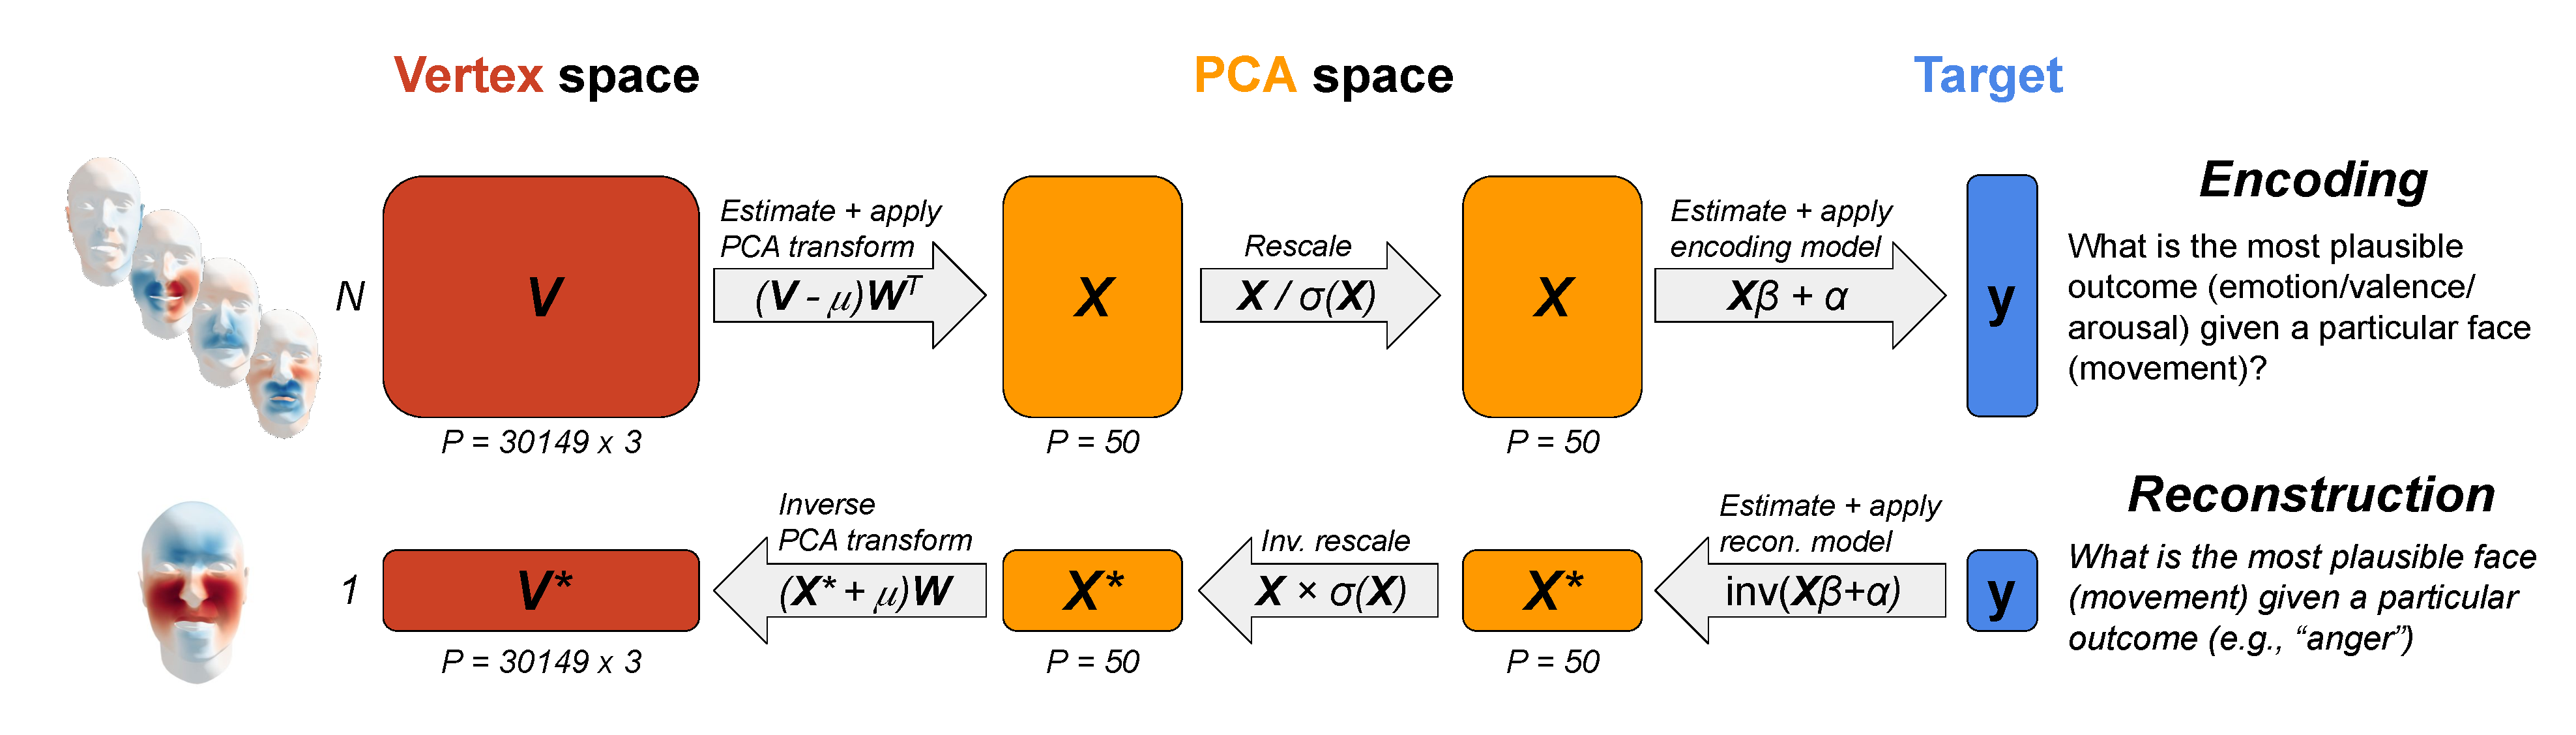
\includegraphics{_bookdown_files/static-vs-dynamic-files/figures/figure_4.pdf}
\caption{\label{fig:fig-svsd-4}Visualization of the encoding (``forward'') model (top) and the reconstruction (``backward'') model (bottom). Note that during the encoding step, a set of \(N\) observations is used to estimate the parameters of the encoding model, while in the reconstruction step only a single observation is reconstructed (although reconstruction can be done for multiple observations at once, if desired).}
\end{figure}



\hypertarget{svsd-code}{%
\subsection{Code availability}\label{svsd-code}}

All code used for the analyses reported in the current study are available on Github: \url{https://github.com/lukassnoek/static-vs-dynamic}. Additionally, code to estimate noise ceilings for both classification and regression models has been released as a Python package, available on Github: \url{https://github.com/lukassnoek/noiseceiling}. The code used for this project makes frequent use of the Python packages \emph{numpy} (Harris et al., \protect\hyperlink{ref-Harris2020-en}{2020}), \emph{pandas} (McKinney \& Others, \protect\hyperlink{ref-McKinney2011-kl}{2011}), \emph{scikit-learn} (Pedregosa et al., \protect\hyperlink{ref-pedregosa2011scikit}{2011}), \emph{matplotlib} (Hunter, \protect\hyperlink{ref-Hunter2007-at}{2007}), and \emph{seaborn} (Waskom, \protect\hyperlink{ref-waskom2021seaborn}{2021}). The prevalence inference estimates were computed using the \emph{bayesprev} Python module from Ince et al. (\protect\hyperlink{ref-Ince2020-mr}{2020}).

\hypertarget{svsd-results}{%
\section{Results}\label{svsd-results}}

In the next two subsections, we report the model performance of the encoding model and the reconstructions from the reconstruction model.

\hypertarget{encoding-model-performance}{%
\subsection{Encoding model performance}\label{encoding-model-performance}}

Figure \ref{fig:fig-svsd-5} summarizes the average explained variance for each affective property (and, in the context of the categorical emotion analysis, different emotions), separately for the static, dynamic, and combined feature sets. For all affective properties, the model based on the combined feature set explains approximately as much as the sum of the static and dynamic model performance (see Supplementary Figure \ref{fig:fig-svsd-S4}, indicating that static and dynamic features explain unique and additive variance. Moreover, the general pattern of results is very similar to (and thus replicates) the results obtained on the optimization set (see Supplementary Figure \ref{fig:fig-svsd-S3}. The posteriors of the population prevalence estimates associated with the model performance scores are visualized in Figure \ref{fig:fig-svsd-6}.

\begin{figure}
\centering
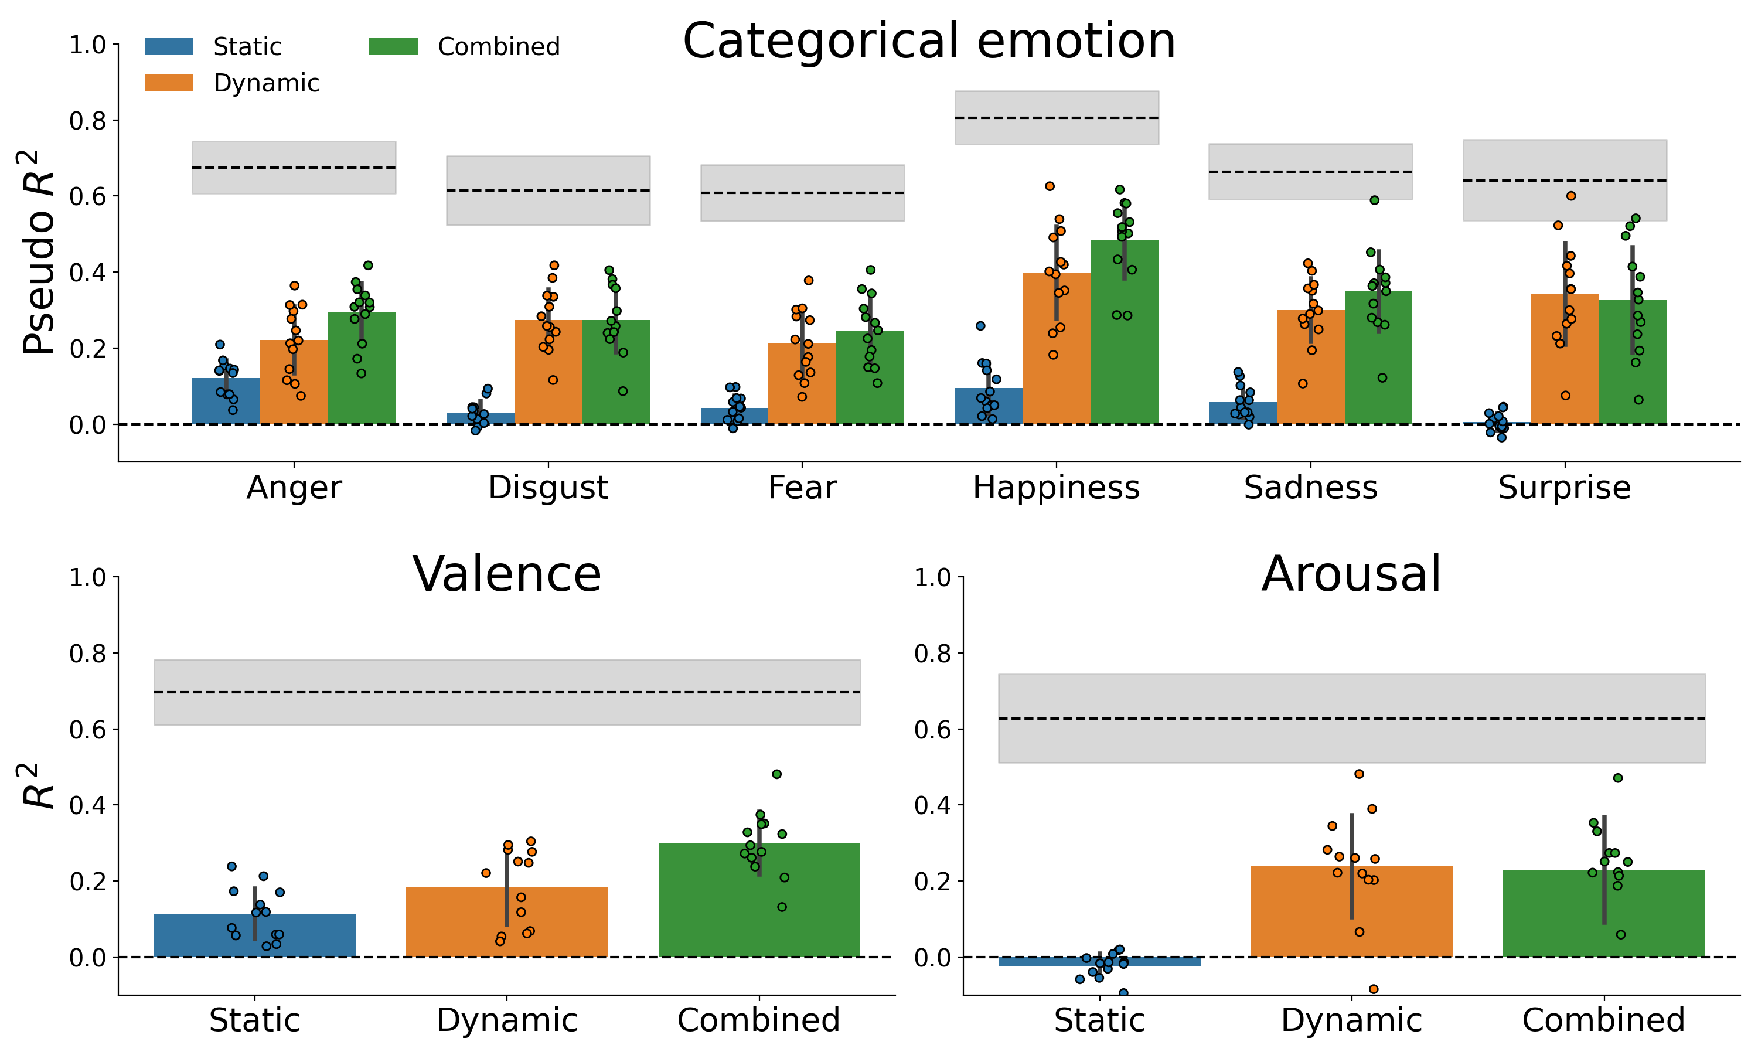
\includegraphics{_bookdown_files/static-vs-dynamic-files/figures/figure_5.pdf}
\caption{\label{fig:fig-svsd-5}Cross-validated model performance, shown separately for each target feature (top: categorical emotion, bottom left: valence, bottom right: arousal) and feature set (static, dynamic, and combined). The bar height represents the mean model performance across participants and the error bars represent ±1 SD. The average within-participant noise ceiling of the \emph{combined} feature set is plotted for reference as a dashed black line, which is surrounded by a grey area indicating ±1 SD.}
\end{figure}



\hypertarget{categorical-emotion-model}{%
\subsubsection{Categorical emotion model}\label{categorical-emotion-model}}

In the categorical emotion analysis, on average about 5.8\% of the variance can be explained by static features (versus 29.1\% by dynamic features and 33.1\% by the combined feature set). The highest percentages explained variance per emotion were observed for anger (12.1\%) and happiness (9.4\%), which were significantly higher than the percentages for the other emotions (evaluated using a paired samples \emph{t}-test, all \emph{p} \textless{} 0.05). The magnitude of the average cross-validated pseudo \(R^2\) scores is roughly proportional to the expected proportion of the population to show an effect (i.e., a cross-validated pseudo \(R^{2}\) significantly larger than 0), as is shown in Figure \ref{fig:fig-svsd-6}. The population prevalence estimates across emotions range from 23\% (for surprise) to 100\% (for anger). For the dynamic and combined model, an effect is expected in the entire population (i.e., a population prevalence of 100\%).

\hypertarget{valencearousal-models}{%
\subsubsection{Valence/arousal models}\label{valencearousal-models}}

Relative to the averaged predictive power of the static features for the categorical emotion model, the predictive power of static features is higher in the valence model, in which it explains on average 11.4\% of the variance (versus 18.3\% using dynamic features and 30.0\% using the combined feature set). This is substantially lower in the arousal model, in which negative \(R^{2}\) values are observed when using static features (versus 23.9\% using dynamic features and 22.9\% using the combined feature set). The computed population prevalence estimates confirm that a statistically significant effect is expected in virtually the entire population for all valence and arousal models, with the exception of the static arousal model, in which an effect is only expected in 30\% of the population).

\begin{figure}
\centering
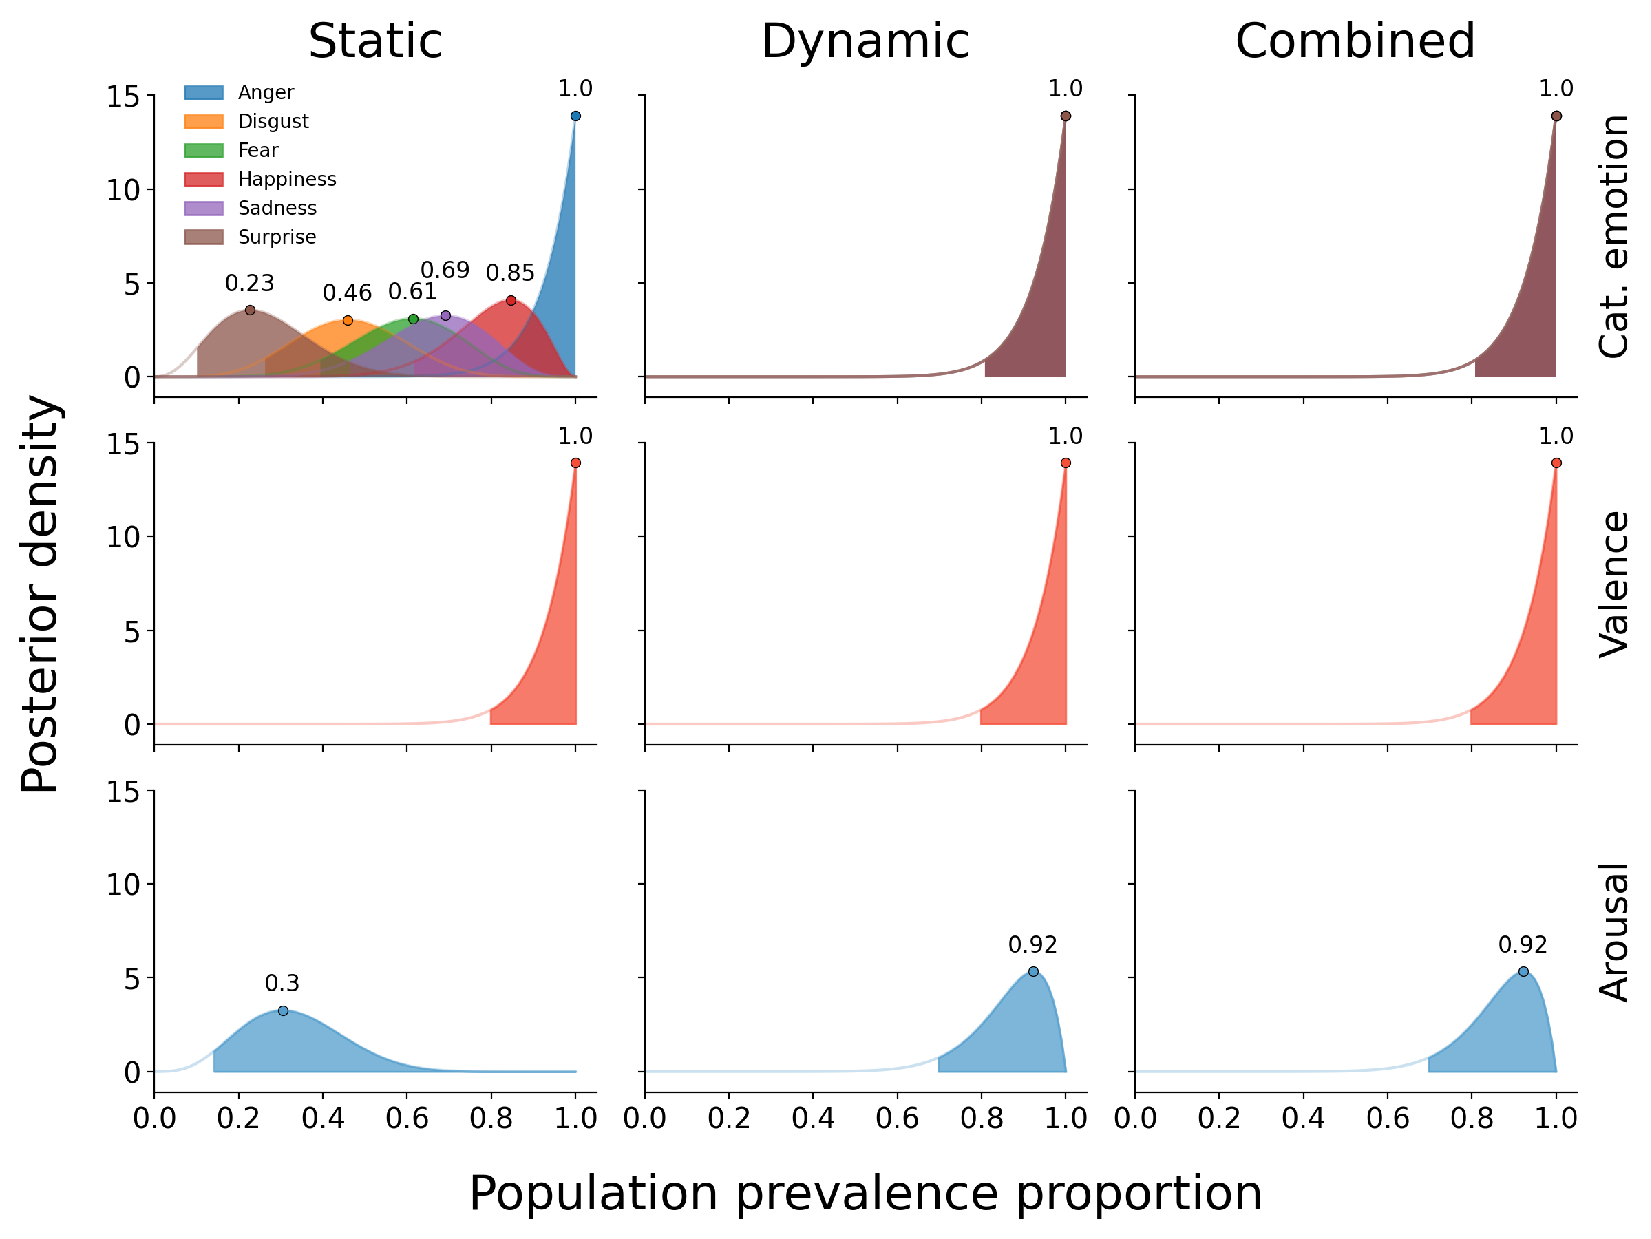
\includegraphics{_bookdown_files/static-vs-dynamic-files/figures/figure_6.pdf}
\caption{\label{fig:fig-svsd-6}The posterior distributions for the population prevalence proportion of the results from the categorical emotion (top), valence (middle), and arousal models (bottom). The posteriors for the different emotions with respect to the dynamic and combined categorical emotion model performances completely overlap, so only a single posterior is shown. The filled area represents the probability density higher than the lower bound of the 96\% highest density interval (McElreath, \protect\hyperlink{ref-McElreath2020-pz}{2020}).}
\end{figure}



\hypertarget{reconstruction-model-visualizations}{%
\subsection{Reconstruction model visualizations}\label{reconstruction-model-visualizations}}

Using the estimated coefficients from the encoding models, we estimated the most likely dynamic and static stimulus features for a given categorical emotion or valence/arousal level. In Figure \ref{fig:fig-svsd-7}, we visualize these reconstructions.

\hypertarget{categorical-emotion-reconstructions}{%
\subsubsection{Categorical emotion reconstructions}\label{categorical-emotion-reconstructions}}

Based on a qualitative visual assessment, the reconstructions from the categorical emotion model based on dynamic information conform to the stereotypical facial expressions associated with categorical emotions (cf.~Ekman et al., \protect\hyperlink{ref-Ekman1969-pu}{1969}; Jack et al., \protect\hyperlink{ref-Jack2016-jq}{2016}). As can be seen in Figure \ref{fig:fig-svsd-8}, anger is associated with a jaw drop, narrowing of the face, raised cheeks, and a lowered brow; disgust is associated with a raised upper lip, raised cheeks, and tightened eyelids; fear is associated with a strong jaw drop and brow raise; happiness is associated with a raised cheeks (which also widens the face), tightened eyelids, and slightly raised eyebrows; sadness is associated with pressed lips, widening of the cheeks, and closed eyes; and surprise is associated with a jaw drop, narrowing of the face and raised eyebrows. Although no stereotypical face structures have been proposed in the literature, the majority of the static reconstructions still show clear and interpretable facial features for most categorical emotions. Anger is associated with a relatively wide face, high forehead, and a protruding nose and chin; disgust is associated with an asymmetric face (in the left-right direction) and protruding mouth/lips; fear is associated with a relatively narrow face and turned-up nose, and slightly protruding mouth; happiness is associated with turned-up mouth corners and high cheekbones; and sadness is associated with a relatively long face and protruding eyebrows. We retrain from interpreting the reconstruction of the static surprise face because static features were not found to be predictive for surprise (see Figure \ref{fig:fig-svsd-5}).

In addition to qualitatively assessing the reconstructions separately, we also compared them quantitatively to each other. In Figure \ref{fig:fig-svsd-8} (top left), we visualize the correlation matrix of the dynamic categorical emotion reconstructions. This correlation matrix shows relatively high correlations between reconstructions of ``anger'' and ``disgust'' (\(r = .62\)) as well as ``surprise'' and ``fear'' (\(r = .56\)), which may underlie the relative frequent confusion between those pairs of emotions (see Supplementary Figure \ref{fig:fig-svsd-S5}, top left). The correlation matrix of the static categorical emotion reconstructions (Figure 9, middle left), in contrast, shows no clear similarities across reconstructions. Finally, we computed the correlation (for each emotion pair) between the static and dynamic reconstructions, which indicates the extent to which static and dynamic share the same ``face topology''. If dynamic and static reconstructions are in fact similar in terms of face topology, we would expect high values on the diagonal of the matrix and low values elsewhere. This actual correlation matrix (Figure \ref{fig:fig-svsd-8}, bottom left), however, does not show this pattern; all correlations between the dynamic and static reconstructions are around 0.

\begin{figure}
\centering
\includegraphics{_bookdown_files/static-vs-dynamic-files/figures/figure_7.pdf}
\caption{\label{fig:fig-svsd-7}The results from the Bayesian reconstruction approach for each emotion from the categorical emotion model and for seven levels, -0.6, -0.4, -0.2, 0, +0.2, +0.4, and +0.6, of the valence and arousal model, shown separately for the static and dynamic feature sets. Color saturation is proportional to the movement or deviation in vertex space (in \emph{SD}).}
\end{figure}



\hypertarget{valencearousal-reconstructions}{%
\subsubsection{Valence/arousal reconstructions}\label{valencearousal-reconstructions}}

The reconstructions from the dynamic valence model also show clear facial movements for both highly negative and highly positive valence values. A face that is experienced as highly negative is associated with an ``inward'' jaw drop, narrowing of the face, and raised cheeks, while a face that is experienced as highly positive is associated with a widening of the face through the cheeks and a raised brow. The reconstructions from the model based on static information shows that faces experienced as highly negative have a wide (``strong'') jawline, a relatively long face, wide forehead, and a protruding brow and mouth, while faces experienced as highly positive have a relatively narrow and short forehead, high cheekbones and mouth corners, and a relatively ``flat'' face (i.e., positive deviations in the \emph{Z} dimension at the edges of the face).

The reconstructions from the arousal model based on dynamic information show that faces eliciting low arousal are associated with a widening of the face, tightening of the lips, and tightened/closed eyes, while faces eliciting high arousal are associated with a strong jaw drop, widening of the eyes, and raised cheeks. The reconstructions from the arousal model based on static information, on the other hand, show less interpretable facial features, which is expected based on the low (below-chance) model performance of the static arousal model.

As can be seen in figure \ref{fig:fig-svsd-7}, the reconstructed faces are highly similar across different magnitudes of valence and arousal, respectively. A strongly positive reconstruction, for example, looks almost the same as a weakly positive one. This suggests that the mental representations of these variables seems to be ``binary'', even though the variables were measured on a continuous (bipolar) scale and the distribution of the ratings is far from binary (see Supplementary Figure \ref{fig:fig-svsd-S2}). Moreover, the ``switching point'' (corresponding to a neutral mental representation) is in some cases offset compared to the midpoint of the rating scale (corresponding to a neutral rating), suggesting a discrepancy between the neutral point of the rating scale and people's mental representation of a ``neutral'' face. Note that this phenomenon is less clearly present in the static arousal reconstructions, but given that the static information was not predictive of arousal ratings, we refrain from interpreting these results.

Finally, given the uniformly low correlation values in the cross-correlation matrix between dynamic and static reconstructions of both valence and arousal (Figure \ref{fig:fig-svsd-8}, bottom center and bottom right), it can be concluded that there does not seem to be any correspondence in face topology between static and dynamic representations of valence and arousal.

\begin{figure}
\centering
\includegraphics{_bookdown_files/static-vs-dynamic-files/figures/figure_8.pdf}
\caption{\label{fig:fig-svsd-8}Correlations between reconstructions in vertex space for the categorical emotion (left), valence (middle), and arousal (right) models. The top row shows the correlations across all dynamic reconstructions. The middle row shows the correlations across all static reconstructions. The bottom row shows the correlations across each combination of a single dynamic and static reconstruction (e.g., in the bottom left correlation matrix, the top right cell represents the correlation between the static anger and the dynamic surprise reconstruction).}
\end{figure}



\hypertarget{correlations-between-affective-properties}{%
\subsubsection{Correlations between affective properties}\label{correlations-between-affective-properties}}

Finally, we evaluated the cross-correlations between the reconstructions of different affective properties. In other words, we evaluate correlations between the reconstructions for different levels of experienced valence and arousal in the observer with the reconstructions for perceived emotions in the face of the expressor (e.g., anger). The correlation matrix of the dynamic reconstruction correlations are visualized in Supplementary Figure \ref{fig:fig-svsd-S8} and the correlation matrix of the static reconstruction correlations are visualized in Supplementary Figure \ref{fig:fig-svsd-S9}. In these correlation matrices, a clear pattern emerged. Specifically, positive valence reconstructions correlated positively with happiness and negative valence reconstructions correlated positively with negative categorical emotion reconstructions (anger, disgust, and fear). Also, low arousal reconstructions correlated positively with happiness and sadness and high arousal reconstructions correlated positively with negative categorical emotion reconstructions (anger, disgust, and fear). Notably, this pattern is both present in the dynamic reconstructions (Supplementary Figure \ref{fig:fig-svsd-S8}) and static reconstruction (Supplementary Figure \ref{fig:fig-svsd-S9}). These findings may explain the previously discussed observations that valence and arousal reconstructions seem to be binary instead of graded. Participants may experience a face as categorically positive when a face displays happiness and as categorically negative when a face displays anger, disgust, or fear. Similarly, participants may experience a face as categorically highly arousing when a face displays anger, disgust, or fear and as categorically low arousing when a face displays happiness or sadness.

\hypertarget{svsd-discussion}{%
\section{Discussion}\label{svsd-discussion}}

In the current study, we sought to quantify and disentangle the importance of dynamic features (facial movement) and static features (facial morphology) on affective face perception. Specifically, using machine learning models based on either dynamic features, static features, or a combination thereof, we aimed to predict categorical emotion, valence, and arousal ratings from a psychophysics experiment with dynamic facial expression stimuli that randomly varied in both their facial movements and facial morphology. To gain further insight into the facial features that are important for prediction of the investigated affective properties, we reconstructed the mental representation of faces associated with the different categorical emotions and different levels of experienced valence and arousal using a multivariate reverse correlation method. In what follows, we discuss the current study's main findings and how they may inform and complement studies on affective face perception.

\hypertarget{facial-morphology-independently-contributes-to-affective-face-perception}{%
\subsection{Facial morphology independently contributes to affective face perception}\label{facial-morphology-independently-contributes-to-affective-face-perception}}

Our models were able to predict human ratings of perceived categorical emotions and elicited valence substantially above chance level using both dynamic and static features. This demonstrates that not only dynamic but also static features of the face determine in what way people perceive and are affected by facial expressions. Moreover, the sum of the dynamic and static model performance scores approximately equals the combined model performance score for all affective properties, which further indicates that the static and dynamic feature sets carry \emph{independent} information that is integrated during perception.

The findings of this study have both fundamental and practical implications for (research on) affective face perception. In general, this study shows that the way we perceive and are affected by faces goes beyond what those faces explicitly communicate. Because static features are by definition unrelated to the expressor's affective state or intentions, one way to frame our findings is that people are biased by features related to facial morphology, perhaps mediated by stereotypes associated with certain demographic groups (e.g., males are thought to display anger more frequently than women; Brooks et al., \protect\hyperlink{ref-Brooks2018-ao}{2018}). In contrast to this interpretation, this ``bias'' could in fact reflect a \emph{true} association between morphological features and the frequency of particular affective expressions (e.g., categorical emotions) or predispositions (e.g., dominance; Zebrowitz, \protect\hyperlink{ref-Zebrowitz2017-qe}{2017}). For example, research has shown that facial width-to-height ratio (FWHR) is associated with aggressive behavior (Lefevre et al., \protect\hyperlink{ref-Lefevre2014-vo}{2014}), which may mediate the relationship between FHWH and anger perception (see Figure \ref{fig:fig-svsd-7}; Deska et al., \protect\hyperlink{ref-Deska2018-hx}{2018}). As this debate about the accuracy of the association between facial morphology and affective predispositions is far from solved (see e.g., Jaeger, Oud, et al., \protect\hyperlink{ref-Jaeger2020-sr}{2020}; Jaeger, Sleegers, et al., \protect\hyperlink{ref-Jaeger2020-bn}{2020}), we leave speculation about this topic to future research that more directly investigates this issue.

On a more practical level, because both static and dynamic features contribute independently to the perception of categorical emotion and experience of valence, researchers studying categorical emotion or valence should use dynamic stimuli of facial expressions instead of static stimuli (i.e., images), which is most commonly done (Krumhuber et al., \protect\hyperlink{ref-Krumhuber2013-qi}{2013}). By using dynamic stimuli, possible effects of static features can be controlled or explicitly adjusted for. This ``decorrelation'' of static and dynamic information is important if one wants to say something about the (unconfounded) effect of static or dynamic information in affective face perception. Given our results, dynamic stimuli are also likely to be more effective for eliciting and modelling arousal, which is in line with previous studies that show that arousal is experienced more intensely in response to dynamic than static stimuli (Sato \& Yoshikawa, \protect\hyperlink{ref-Sato2007-ah}{2007}).

\hypertarget{the-influence-of-facial-morphology-does-not-result-from-visual-similarity-to-facial-movements}{%
\subsection{The influence of facial morphology does not result from visual similarity to facial movements}\label{the-influence-of-facial-morphology-does-not-result-from-visual-similarity-to-facial-movements}}

Contrary to what is often reported in previous studies (Hess, Adams, \& Kleck, \protect\hyperlink{ref-Hess2009-xo}{2009}; Said et al., \protect\hyperlink{ref-Said2009-tf}{2009}; Zebrowitz, \protect\hyperlink{ref-Zebrowitz2017-qe}{2017}), we do not find that static and dynamic features visually resemble each other, as is evident from the low correlations between static and dynamic reconstructions for each categorical emotion and valence and arousal levels. Instead, the static reconstructions show qualitatively different facial features for each emotion and valence/arousal level relative to the dynamic reconstructions. For example, the static anger reconstruction shows a relatively strong jawline (cf.~Deska et al., \protect\hyperlink{ref-Deska2018-hx}{2018}), high forehead, and protruding nose and chin, while the dynamic anger reconstruction shows a narrowing of the face, raised cheeks, and lowered brow. Many of the facial features associated with static reconstructions are similar to facial features associated with social judgments. For example, the strong jawline we observe in the static anger reconstruction has been associated with the perception of dominance (Mileva et al., \protect\hyperlink{ref-Mileva2014-ld}{2014}; Windhager et al., \protect\hyperlink{ref-Windhager2011-ik}{2011}) and the pronounced cheekbones we observe in the static happiness reconstruction has been associated with the perception of trustworthiness (Oosterhof \& Todorov, \protect\hyperlink{ref-Oosterhof2009-mf}{2009}; Todorov et al., \protect\hyperlink{ref-Todorov2008-eb}{2008}). This suggests that the effect of static features on categorical emotion perception may be mediated by social attributions such as dominance and trustworthiness (Adams et al., \protect\hyperlink{ref-Adams2012-dl}{2012}; Craig et al., \protect\hyperlink{ref-Craig2017-db}{2017}; Gill et al., \protect\hyperlink{ref-Gill2014-hx}{2014}; Hess, Adams, et al., \protect\hyperlink{ref-Hess2009-br}{2009}; Montepare \& Dobish, \protect\hyperlink{ref-Montepare2003-hy}{2003}). However, the difference between our findings and previously reported associations between social attributions and categorical emotion perception (with the exception of Gill et al., \protect\hyperlink{ref-Gill2014-hx}{2014}) is that we show that the static features we found to be important for categorical emotion perception do not resemble dynamic features usually associated with particular emotion expressions.

\hypertarget{categorical-representations-of-experienced-valence-and-arousal-correlate-with-representations-of-perceived-emotions}{%
\subsection{Categorical representations of experienced valence and arousal correlate with representations of perceived emotions}\label{categorical-representations-of-experienced-valence-and-arousal-correlate-with-representations-of-perceived-emotions}}

Furthermore, the qualitative and quantitative analyses of the reconstructions at different valence and arousal levels shows that even though valence and arousal were measured at a continuous scale, participants seem to represent valence and arousal in a categorical fashion, i.e., as either positive or negative valence and as either low or high arousal. An intriguing potential explanation for this finding is that the valence and arousal experiences of participants may be directly tied to the categorical emotions perceived in the face. Indeed, for both dynamic and static reconstructions, the correlations between the positive valence reconstructions and the happiness reconstruction and the negative valence reconstructions and the anger, disgust, and fear reconstructions are substantial (see Supplementary Figure \ref{fig:fig-svsd-S8}-\ref{fig:fig-svsd-S9}. Likewise, the correlations between low arousal reconstructions and the happiness and sadness reconstructions and high arousal reconstructions and the anger, disgust, and fear reconstructions are substantial. Thus, an individual's affective response to a face may stem from the face's similarity to the observer's representation of categorical emotions.

\hypertarget{predictive-models-quantify-what-is-not-yet-known}{%
\subsection{Predictive models quantify what is (not yet) known}\label{predictive-models-quantify-what-is-not-yet-known}}

The current study used a predictive modelling approach (as opposed to null-hypothesis significance testing used in most previous research) to precisely quantify and compare the importance of static and dynamic information in affective face perception. In addition, using the concept of a noise ceiling, we showed that although a substantial proportion of the variance in ratings can be explained, the difference between the average model performance and the noise ceiling indicates that there is room for improvement. As our models were all linear and additive, one possibility for improvement is the use of non-linear models, which may capture possible many-to-one mappings between facial movements and affective properties (Snoek et al., \protect\hyperlink{ref-snoek-submitted}{n.d.}). The recent successes of computer vision algorithms (which are usually highly non-linear) in emotion classification indicate that this avenue may be promising (Ko, \protect\hyperlink{ref-Ko2018-rv}{2018}). Another possibility for improving predictive model performance is to enrich the static and dynamic feature spaces. For example, one could consider static features beyond facial morphology, such as facial texture (Punitha \& Geetha, \protect\hyperlink{ref-Punitha2013-jy}{2013}; Xie \& Lam, \protect\hyperlink{ref-Xie2009-fp}{2009}) and color (Benitez-Quiroz et al., \protect\hyperlink{ref-Benitez-Quiroz2018-vr}{2018}; Thorstenson et al., \protect\hyperlink{ref-Thorstenson2018-io}{2018}). Investigating alternative algorithms and additional or different feature spaces, which can be evaluated by their predictive accuracy, may generate a more complete and accurate model of affective face perception.

\hypertarget{limitations-and-further-directions}{%
\subsubsection{Limitations and further directions}\label{limitations-and-further-directions}}

Although we believe the current study yields important insights into the role of static and dynamic information in affective face perception, it suffers from several limitations that affect its generalizability, which in turn provides directions for future research. First, we specifically investigated categorical emotion as an affective state of the expressor and valence/arousal as an affective experience of the observer, but this covers only a part of the possibilities. Future studies could additionally investigate how static and dynamic information are related to categorical emotions as an affective state of the observer and valence/arousal as an affective state of the expressor. Second, although we investigated multiple affective properties of the face, they do not capture affective face perception in its full complexity. For example, the six basic categorical emotions we investigated are a subset of a larger range of known categorical affective states (Cowen et al., \protect\hyperlink{ref-Cowen2021-ld}{2021}; Cowen \& Keltner, \protect\hyperlink{ref-Cowen2017-vz}{2017}). Future research could use the approach from the current study to investigate whether the largely independent contribution of static and dynamic information holds for affective states beyond those investigated in the current study. Second, although our psychophysics approach samples the space of dynamic and static information more extensively than most studies, the stimulus set we used remains limited. Although random sampling of facial movements ensures that analyses and subsequent results are relatively unbiased by existing theoretical considerations (Jack et al., \protect\hyperlink{ref-Jack2017-qp}{2017}), they may yield facial expressions that are unlikely to be encountered in daily life. As a consequence, these facial expressions may be rated relatively inconsistently and subsequently bias model performance downwards. In addition, our stimulus set was generated to optimize for variance in facial movements. As such, while our stimulus set covers a large part of the space of possible facial movements, it is unclear to what degree the fifty different faces in our stimulus set cover the range of variation in facial morphology. Specifically, to improve the variance in static features, future studies could benefit from including faces from different ethnicities and a wider age range, which may in turn improve generalizability of the results.

\hypertarget{svsd-conclusion}{%
\section{Conclusion}\label{svsd-conclusion}}

In this study, we show that both dynamic information (i.e., facial movements) and static information is integrated during affective face perception, and that these sources of information are largely independent. This finding demonstrates that people extract more from the face than is intentionally or unintentionally communicated. Importantly, these results in general raise concerns about using static images (rather than videos) in facial expression research or automated facial expression recognition systems, because (apparent) dynamic and static information are fundamentally confounded in images. We hope that our data-driven, predictive approach paves the way for future research that embraces the face as a communicator and elicitor of affective states in all its complexity.

\hypertarget{general-discussion}{%
\chapter{Discussion}\label{general-discussion}}

Psychology and cognitive neuroscience are relatively young scientific fields. Using the empirical cycle, these fields have developed and tested many different theories about the human mind and brain over the years, almost exclusively by means of hypothesis testing. In the past twenty years or so, we have seen a (renewed) interest in a more computational, predictive approach that is used in addition and complementary to the traditional hypothesis testing approach (Yarkoni \& Westfall, \protect\hyperlink{ref-Yarkoni2017-om}{2017}). In this thesis, inspired by techniques and models from machine learning, I explored how this predictive approach can be applied and adapted to behavioral research (chapter \ref{hypothesis-kernel-analysis} and \ref{static-vs-dynamic}) and neuroimaging research (chapter \ref{shared-states} and \ref{confounds-decoding}). This thesis also addresses the importance of large, publicly accessible datasets, an example of which is described in chapter \ref{aomic}. Finally, highlighting the fact that arguably the most effective scientific methodology embraces both predictive modelling and hypothesis testing, chapter \ref{morbid-curiosity} outlined an example of a fully preregistered, confirmatory neuroimaging study. In the \protect\hyperlink{general-introduction}{general introduction} to this thesis, I described how predictive modelling can complement the hypothesis testing approach in psychology and cognitive neuroscience; in what follows, I will outline what I think is necessary to facilitate the adoption of this approach.

An important step in the adoption of a ``predictive approach'' is changing the way we derive research questions and hypotheses. The hypothetico-deductive tradition in psychology and cognitive neuroscience has taught us that research questions should be based on theories that, ideally, can be answered using statistical tests of binary hypotheses (Kellen, \protect\hyperlink{ref-Kellen2019-af}{2019}). The consequence of this approach is that research questions only capture a very specific part of a target system. Instead, I believe we should steer our research questions towards the mechanisms behind particular cognitive capacities and behaviors (Rooij \& Baggio, \protect\hyperlink{ref-Van_Rooij2021-bk}{2021}). For example, instead of investigating whether certain categorical emotions are universally recognized, one could try to construct a model of emotion recognition and show if and how culture affects this model (Jack et al., \protect\hyperlink{ref-Jack2009-yy}{2009}). As chapter \ref{shared-states} in this thesis shows, however, studies may feature both hypothesis tests as well as (elements of) predictive models. I think that if one aims to adopt a predictive approach, a good rule of thumb is to ask oneself whether the research question can be answered with ``yes'' or ``no''; if that is the case, I would recommend to try to rephrase the question such that the research question revolves around the word ``how'' and cannot be answered using a simple ``yes'' or ``no'' answer.

Adopting a more predictive approach also means that we should perhaps not let theory guide our research as much as in the hypothesis testing approach. Of course, theories may inspire elements of predictive models (e.g., constructionism tells us that we should not limit our models of emotion to perceptual inputs only; Barrett et al., \protect\hyperlink{ref-Barrett2019-bc}{2019}), but they should not determine all aspects of the study design, experiment, and statistical model (Jack et al., \protect\hyperlink{ref-Jack2017-qp}{2017}). Instead, the data used for predictive modelling, whether that is observational or experimental data, should ideally allow for exploration and comparison of different models (Gelfert, \protect\hyperlink{ref-Gelfert2016-hd}{2016}). This way, the ``information gain'' from a single experiment or study can be much higher than when conducting a single hypothesis test.

The exploratory mindset of the predictive modelling approach calls for a different way to think about the data that we use for our models. In hypothesis testing, we usually want to limit our inferences to a single factor, which we explicitly manipulate in our experiments. For predictive modelling, on the other hand, the data should ideally vary in all the dimensions that are relevant for the capacity or behavior that is investigated. These ``rich'' datasets do not only allow for more exploration and a better generalizability, but are also less constrained (or ``biased'') a priori by existing theories (Jack et al., \protect\hyperlink{ref-Jack2017-qp}{2017}). Chapter \ref{static-vs-dynamic} provides an illustrative example of an experimental approach to create datasets that are relatively rich and unbiased by theory. In this study, we used a ``social psychophysics'' approach (Jack \& Schyns, \protect\hyperlink{ref-Jack2017-gt}{2017}) to create facial expression stimuli that randomly varied in both facial movements (sampled uniformly from a large set of ``action units'') as well as facial morphology (sampled from a large database of individuals). This allowed us to explore different models based on dynamic features (i.e., facial movement) and compare these to models based on static features (i.e., facial morphology).

The development of such rich datasets, however, may pose practical problems. One prominent issue is that, with each additional dimension that is considered, the space of the data grows exponentially, a phenomenon known as the ``curse of dimensionality''. With increasingly higher dimensional spaces, randomly sampling data quickly becomes practically infeasible. One solution for this issue is to constrain the (co)variance of the data using prior information, like we did in chapter \ref{static-vs-dynamic} by restricting facial movements to those that have been consistently shown to be important in affective face perception. For observational data, constraints on (random) sampling can also be achieved by the use of ``naturalistic'' or ``ecologically valid'' data, which has been increasingly popular in cognitive neuroscience (Nastase et al., \protect\hyperlink{ref-Nastase2020-he}{2020}).

Rich and naturalistic datasets by themselves are, however, not enough. Like machine learning researchers have done in computer vision with datasets such as ImageNet, we should strive to collaboratively create large, rich, and importantly \emph{publicly available} datasets that can be used as benchmarks for the development and evaluation of predictive models. An important prerequisite for this endeavor is that research communities can agree on which particular cognitive capacity or behavior should be targeted, how to operationalize this, and which stimulus or task dimensions should be sampled (Adjerid \& Kelley, \protect\hyperlink{ref-Adjerid2018-vs}{2018}). Although focused on hypothesis testing instead of predictive modelling, initiatives such as the \emph{Psychological Science Accelerator} (Moshontz et al., \protect\hyperlink{ref-Moshontz2018-rc}{2018}) and the different \emph{ManyLabs} projects (Ebersole et al., \protect\hyperlink{ref-Ebersole2016-cr}{2016}; Klein et al., \protect\hyperlink{ref-Klein2018-un}{2018}) have shown that such large-scale efforts are possible. Moreover, I think that competitions and challenges centered around these benchmark datasets can lead to rapid progress in explanation and understanding of specific cognitive capacities and behaviors, like ImageNet has done for object recognition.

The development of rich datasets afford the use of more complex predictive models, which in my opinion are necessary to capture the complex, high-dimensional nature of cognitive capacities and behavior (Jolly \& Chang, \protect\hyperlink{ref-Jolly2019-lx}{2019}). Complexity, here, can mean two things. One interpretation of model complexity refers to the high dimensionality of models, i.e., models that work with data with many predictors. These high-dimensional inputs may either be directly measured or computationally derived from the data, which are subsequently related to the target variable using a (linear) model. An example of the former strategy in the context of neuroimaging is a ``decoding model'', which aims to relate high-dimensional patterns of brain data to experimental features (see Chapter \ref{shared-states} and \ref{confounds-decoding}). In my opinion, the latter strategy that uses a computational model to explicitly derive model features is more promising. In cognitive neuroscience, such computational models are known as ``linearizing models'' (Naselaris et al., \protect\hyperlink{ref-Naselaris2011-oh}{2011}), because the model relates features resulting from a potentially non-linear computational model to the target variable using a linear model (i.e., the approach \emph{linearizes} the mapping from input to the target variable). We used this approach in chapter \ref{static-vs-dynamic}, in which we used a computational model from computer vision (a 3D morphable model; Yu et al., \protect\hyperlink{ref-Yu2012-ag}{2012}) to generate facial shape features which were subsequently used to predict categorical emotion, valence, and arousal ratings using a logistic regression model.

Another, and more common, interpretation of model complexity is related to the number of model parameters. In the past, models usually limited the number of parameters to prevent overfitting, but the increase in available data and compute power in the 21st century enabled training models with an increasingly larger number of parameters. The most popular class of models resulting from these developments are known as ``deep learning'' models, a type of artificial neural network that maps inputs to outputs using a series of non-linear transformations (LeCun et al., \protect\hyperlink{ref-LeCun2015-xa}{2015}). Deep learning models represent the state-of-the-art in almost all domains of artificial intelligence, including object recognition, reinforcement learning, and natural language processing (Maas et al., \protect\hyperlink{ref-Van_der_Maas2021-rx}{2021}). In cognitive neuroscience, too, deep learning models tend to outperform traditional computational vision models in predicting neural activity in response to visual stimuli (Khaligh-Razavi \& Kriegeskorte, \protect\hyperlink{ref-khaligh2014deep}{2014}; Kriegeskorte, \protect\hyperlink{ref-Kriegeskorte2015-qi}{2015}).

As discussed in the general introduction to this thesis, using complex predictive models trained on observational data may feel like trading in one black box (the brain/mind) for another (a model), which does not yield an improved understanding of the investigated target system. This trade-off between \emph{prediction} and \emph{explanation} is to some extent unavoidable but, I would argue, a trade-off worth making. I would rather have a black box with 90\% accuracy than a directly interpretable model with 10\% accuracy. The reason for this preference stems from the fact that a highly predictive model can be used as a ``surrogate'' (or model organism; Scholte, \protect\hyperlink{ref-Scholte2018-he}{2018}) of the target system, which can be inspected, manipulated, and experimented with in order to explain and gain understanding of it. With decades of experience with experimentation and deriving causal insights from empirical research, I think that psychologists and cognitive neuroscientists are superbly equipped for this role.

The development of a research climate that combines the strengths of both the predictive and the hypothesis testing approach is not something that will happen overnight. The predictive approach represents more than a choice of model. It requires a different type of experimental cycle, which revolves less on theory and hypotheses and more on exploration and post-hoc explanation. If we choose to focus more on prediction, we have to start asking different questions (about mechanisms, not effects); we have to embrace the complexity of human cognition and behavior and build datasets and models that reflect this complexity; and we have to sacrifice interpretability for accuracy. Like any break with tradition, this may feel uncomfortable at first, but in doing so, I believe that a promising future lies ahead.

\hypertarget{appendix-appendix}{%
\appendix}


\cleardoublepage
\phantomsection
\addcontentsline{toc}{part}{Appendices}
\appendixpage*
\setlength\beforechapskip{-\baselineskip}

\hypertarget{shared-states-supplement}{%
\chapter{Supplement to Chapter \ref{shared-states}}\label{shared-states-supplement}}

\begingroup\fontsize{10}{12}\selectfont

\begin{ThreePartTable}
\begin{TableNotes}[para]
\item \textit{Note: } 
\item The stimulus materials presented in Table S1 were selected from a pilot study. In this pilot study we asked an independent sample of twenty-four subjects to describe how they would express an emotion in their behavior, body posture or facial expression (action information), what specific sensations they would feel inside their body when they would experience an emotion (interoceptive information), and for what reason or in what situation they would experience an emotion (situational information). These three questions were asked in random order for twenty-eight different negative emotional states, including anger, fear, disgust, sadness, contempt, worry, disappointment, regret and shame. The descriptions generated by these subjects were used as qualitative input in order to create our stimulus set of twenty short sentences that described emotional actions, sensations or situations. With this procedure, we ensured that our stimulus set held sentences that were validated and ecologically appropriate for our sample.
\end{TableNotes}
\begin{longtabu} to \linewidth {>{\raggedright\arraybackslash}p{5em}>{\raggedright}X>{\raggedright}X}
\caption{\label{tab:tab-shared-states-S1}Stimuli used for SF-task}\\
\toprule
Class & Dutch & English translation\\
\midrule
Action & Hard wegrennen & Running away fast\\
 & Iemand wegduwen & Pushing someone away\\
 & Iemand stevig vastpakken & Holding someone tightly\\
 & Je hoofd schudden & Shaking your head\\
 & Heftige armgebaren maken & Making big arm gestures\\
\addlinespace
 & Ergens voor terugdeinzen & Recoiling from something\\
 & Je ogen dichtknijpen & Closing your eyes tightly\\
 & Je ogen wijd open sperren & Opening your eyes widely\\
 & Je wenkbrauwen fronsen & Frowning with your eyebrows\\
 & Je schouders ophalen & Raising your shoulders\\
\addlinespace
 & Op de vloer stampen & Stamping on the floor\\
 & In elkaar duiken & Cowering\\
 & Je schouders laten hangen & Slumping your shoulders\\
 & Je vuisten ballen & Tighten your fists\\
 & Je borst vooruit duwen & Push your chest forward\\
\addlinespace
 & Je tanden op elkaar zetten & Clench your teeth\\
 & Je hand voor je mond slaan & Put your hand in front of your mouth\\
 & Onrustig bewegen & Moving restlessly\\
 & Heen en weer lopen & Walking back and forth\\
 & Je hoofd afkeren & Turning your head away\\
\addlinespace
Interoception & Een brok in je keel & A lump in your throat\\
 & Buiten adem zijn & Being out of breath\\
 & Een versnelde hartslag & A fast beating heart\\
 & Je hart klopt in de keel & You heart is beating in your throat\\
 & Een benauwd gevoel & An oppressed feeling\\
\addlinespace
 & Een misselijk gevoel & Being nauseous\\
 & Druk op je borst & A pressure on your chest\\
 & Strak aangespannen spieren & Tense muscles\\
 & Een droge keel & A dry throat\\
 & Koude rillingen hebben & Cold shivers\\
\addlinespace
 & Bloed stroomt naar je hoofd & Blood is going to your head\\
 & Een verdoofd gevoel & A numb feeling\\
 & Je hebt tintelende ledenmaten & Tingling limbs\\
 & Een verlaagde hartslag & A slow heartbeat\\
 & Je hebt zware ledematen & Heavy limbs\\
\addlinespace
 & Een versnelde ademhaling & Fast breathing\\
 & Je hebt hoofdpijn & Headache\\
 & Je hebt buikpijn & Stomachache\\
 & Zweet staat in je handen & Sweaty palms\\
 & Je maag keert zich om & Your stomach churns\\
\addlinespace
Situation & Vals beschuldigd worden & Being falsely accused\\
 & Dierbare overlijdt & A loved one dies\\
 & Vlees is bedorven & Meat that has gone off\\
 & Je wordt bijna aangereden & You are almost hit by a car\\
 & Iemand naast je braakt & Someone next to you vomits\\
\addlinespace
 & Huis staat in brand & House is on fire\\
 & Zonder reden ontslagen worden & Being fired for no reason\\
 & Een ongemakkelijke stilte & An uncomfortable silence\\
 & Alleen in donker park & Alone in a dark park\\
 & Inbraak in je huis & A house burglary\\
\addlinespace
 & Een gewond dier zien & Seeing a wounded animal\\
 & Tentamen verknallen & Messing up your exam\\
 & Je partner bedriegt je & You partner cheats on you\\
 & Dierbare is vermist & A loved one is missing\\
 & Belangrijke sollicitatie vergeten & Forgot a job interview\\
\addlinespace
 & Onvoorbereid presentatie geven & Giving a presentation unprepared\\
 & Je baas beledigt je & Your boss offends you\\
 & Goede vriend negeert je & A good friend neglects you\\
 & Slecht nieuws bij arts & Bad news at the doctor\\
 & Bommelding in metro & A bomb alarm in the metro\\
\bottomrule
\insertTableNotes
\end{longtabu}
\end{ThreePartTable}
\endgroup{}

~
~

\textbf{Full instruction for the other-focused emotion understanding task.}

\emph{Translated from Dutch; task presented first.}

"In this study we are interested in how the brain responds when people understand the emotions of others in different ways. In the scanner you will see images that display emotional situations, sometimes with multiple people. In every image one person will be marked with a red square. While viewing the image we ask you to focus on the emotion of that person in three different ways.

With some images we ask you to focus on HOW this person expresses his or her emotion. Here we ask you to identify expressions in the face or body that are informative about the emotional state that the person is experiencing.

With other images we ask you to focus on WHAT this person may feel in his or her body. Here we ask you to identify sensations, such as a change in heart rate, breathing or other internal feeling, that the person might feel in this situation.

With other images we ask you to focus on WHY this person experiences an emotion. Here we ask you to identify a specific reason or cause that explains why the person feels what he or she feels.

Every image will be presented for six seconds. During this period we ask you to silently focus on HOW this person expresses emotion, WHAT this person feels in his/her body, and WHY this person feels an emotion.

Before you will enter the scanner we will practice. I will show you three images and will ask you to perform each of the three instructions out loud.

It is important to note that there are no correct or incorrect answers, it is about how you interpret the image. For the success of the study it is very important that you apply the HOW, WHAT or WHY instruction for each image. Please do not skip any images and try to apply each instruction with the same motivation. It is also important to treat every image separately, although it is possible that you have similar interpretations for different images.
The three instructions are combined with the images in blocks. In every block you will see five images with the same instruction. Each block will start with a cue that tells you what to focus on in that block.

Each image is combined with all three instructions, so you will see the same image multiple times. In between images you will sometimes see a black screen for a longer period of time.

Do you have any questions?"

~
~

\textbf{Full instruction for the self-focused emotion imagery task.}

\emph{Translated from Dutch; task presented second.}

"In this study we are interested in how the brain responds when people imagine different aspects of emotion. In the scanner you will see sentences that describe aspects of emotional experience. We ask you to try to imagine the content of each sentence as rich and detailed as possible.

Some sentences describe actions and expressions. We ask you to imagine that you are performing this action or expression. Other sentences describe sensations or feelings that you can have \emph{inside} your body. We ask you to imagine that you are experiencing this sensation or feeling. Other sentences describe emotional situations. We ask you to imagine that you are experiencing this specific situation.

We ask you to always imagine that YOU have the experience. Thus, it is about imagining an action or expression of your body, a sensation inside your body, or a situation that you are part of.

I will give some examples now.

For each sentence you have six seconds to imagine the content. All sentences will be presented twice. In between sentences you will sometimes see a black screen for a longer period of time. For this experiment to succeed it is important that you imagine each sentence with the same motivation, even if you have seen the sentence before. Please do not skip sentences.

Do you have any questions?"

\begin{figure}
\centering
\includegraphics{_bookdown_files/shared-states-files/figures/figure_S1.pdf}
\caption{\label{fig:fig-shared-states-S1}Mean percentage of trials successfully executed for the SF-task (left panel) and OF-task (right panel). Error bars indicate 95\% confidence intervals. A one-way ANOVA of the success-rates of the SF-task (left-panel) indicated no significant overall differences, \emph{F}(2, 17) = 1.03, p = 0.38. In the OF-task (right panel) however, a one-way ANOVA indicated that success-rates differed significantly between classes, \emph{F}(2, 17) = 17.74, \emph{p} \textless{} 0.001. Follow-up pairwise comparisons (Bonferroni corrected, two tailed) revealed that interoception-trials (\emph{M} = 74.00, \emph{SE} = 2.10) were significantly less successful (\emph{p} \textless{} 0.001) than both action-trials (\emph{M} = 85.50, \emph{SE} = 1.85) and situation trials (\emph{M} = 90.00, \emph{SE} = 1.92).}
\end{figure}



\newpage
\pagestyle{empty}
\blandscape

\begin{figure}
\includegraphics[width=0.9\linewidth,height=0.9\textheight]{_bookdown_files/shared-states-files/figures/figure_S2} \caption{Results of the parameter-optimization procedure. Reported scores reflect the classification scores averaged over subjects and classes (i.e.~the diagonal of the confusion matrix). All optimization analyses were iterated 5000 times. \textbf{A}) Classification results for different smoothing kernels (0, 2, 5, and 10 mm) and z-value threshold for differentiation scores during feature selection (see MVPA pipeline section in the main text for a description of the particular feature selection method we employed). Numbers reflect the average number of voxels selected across iterations. \textbf{B}) Classification results of using a low-pass filter (2 seconds) or not. \textbf{C}) Classification results for different numbers of test-trials per class (1 to 5). \textbf{D}) Classification results when preprocessing the data with Independent Component Analysis (ICA) or not.}\label{fig:fig-shared-states-S2}
\end{figure}



\elandscape
\newpage
\pagestyle{\defstyle}

\begingroup\fontsize{10}{12}\selectfont

\begin{ThreePartTable}
\begin{TableNotes}[para]
\item \textit{Note: } 
\item The first set of parameters we evaluated in the optimization-set were different smoothing factors and feature selection thresholds (see MVPA pipeline section in the main text). On average, across the self- and cross-analysis, a 5 mm smoothing kernel yielded the best results in combination with a feature selection threshold of 2.25, which we rounded up to 2.3 as this number represents a normalized (z-transformed) score, which corresponds to the top 1\% scores within a normal distribution. Next, the difference between using a low-pass (of 2 seconds, i.e. 1 TR) versus none was assessed, establishing no low-pass filter as the optimal choice. Next, different numbers of test-trials (1 to 5) per class per iteration were assessed. Four trials yielded the best results. Lastly, the effect of “cleaning” the data with an independent component analysis was examined (FSL: MELODIC and FIX; Salimi-Khorshidi et al., 2014). Not performing ICA yielded the best results. These parameters – 5 mm smoothing kernel, 2.3 feature selection thresholded, no low-pass filter, and four test-trials per iteration – were subsequently used in the analysis of the validation set.
\end{TableNotes}
\begin{longtabu} to \linewidth {>{\raggedright}X>{\raggedright}X>{\raggedright}X}
\caption{\label{tab:tab-shared-states-S2}Parameters assessed in the optimization set}\\
\toprule
Parameter & Options & Final choice\\
\midrule
Smoothing kernel & 0 mm, 2 mm, 5 mm, 10 mm & 5 mm\\
Feature selection threshold & 1.5, 1.75, 2, 2.25, 2.5, 2.75, 3 & 2.3\\
Number of test-trials & 1, 2, 3, 4, 5 & 4\\
Low-pass filter & 2 seconds vs. none & None\\
ICA denoising & ICA vs. no ICA & No ICA\\
\bottomrule
\insertTableNotes
\end{longtabu}
\end{ThreePartTable}
\endgroup{}

\begin{figure}
\centering
\includegraphics{_bookdown_files/shared-states-files/figures/figure_S3.pdf}
\caption{\label{fig:fig-shared-states-S3}Confusion matrices displaying precision-values yielded by the classification analysis of the optimization dataset with the final set of parameters. Because no permutation statistics were calculated for the optimization set, significance was calculated using a one-sample independent \emph{t}-test against chance-level classification (i.e.~0.333) for each cell in the diagonal of the confusion matrices. Here, all t-statistics use a degrees of freedom of 12 (i.e.~13 subjects - 1) and are evaluated against a significance level of 0.05, Bonferroni-corrected. For the diagonal of the self-analysis confusion matrix, all values were significantly above chance-level, all \emph{p} \textless{} 0.0001. For the diagonal of the cross-analysis confusion matrix, both the action (43\% correct) and situation (44\% correct) classes scored significantly above chance, \emph{p} = 0.014 and \emph{p} = 0.0007 respectively. Interoception was classified at chance level, \emph{p} = 0.99, which stands in contrast with the results in the validation-set.}
\end{figure}



\begin{figure}
\centering
\includegraphics{_bookdown_files/shared-states-files/figures/figure_S4.pdf}
\caption{\label{fig:fig-shared-states-S4}Schematic overview of the bagging procedure. Class probabilities across different bagging iterations are summed and the class with the maximum probability determines each trial's final predicted class, which are subsequently summarized in a confusion matrix on which final recall/precision scores are calculated.}
\end{figure}



\begin{figure}
\centering
\includegraphics{_bookdown_files/shared-states-files/figures/figure_S5.pdf}
\caption{\label{fig:fig-shared-states-S5}A comparison between precision and recall confusion matrices of the self- and cross-analysis of the validation dataset.
Precision refers to the amount of true positive predictions of a given class relative to all predictions for that class. Recall refers to the amount of true positive predictions of a given class relative to the total number of samples in that class. In the self-analysis, all classes were decoded significantly above chance for both precision and recall (all \emph{p} \textless{} 0.001). In the cross-analysis, all classes were decoded significantly above chance for precision (all \emph{p} \textless{} 0.001); for recall both action and situation were decoded significantly above chance (\emph{p} = 0.0013 and \emph{p} \textless{} 0.001, respectively), while interoception was decoded below chance. All \emph{p}-values were calculated using a permutation test with 1300 permutations (as described in the Methods section in the main text). When comparing precision and recall scores for both analyses, precision and recall showed very little differences in the self-analysis, while the cross-analysis shows a clear difference between metrics, especially for interoception and situation. For the interoception class, the relatively high precision score (44\%) compared to its recall score (14\%) suggests that trials are very infrequently classified as interoception, but when they are, it is (relatively) often correct. For the situation class, the relatively high recall score (72 \%) compared to its precision score (44\%) suggests that situation is strongly over-classified, which is especially clear in the lower-right confusion matrix, which indicates that 59\% of the interoception-trials are misclassified as situation-trials.}
\end{figure}




\begin{figure}
\centering
\includegraphics{_bookdown_files/shared-states-files/figures/figure_S6.pdf}
\caption{\label{fig:fig-shared-states-S6}Relation between self- and cross-analysis scores across subjects and their respective distributions. Note that the scores here represent the average of the class-specific precision scores. \textbf{A}) There is no significant correlation between precision-scores on the self-analysis and the corresponding scores on the cross-analysis, \emph{r} = -0.04, \emph{p} = .86, implying that classification scores in the self-analysis is not predictive of scores in the cross-analysis. \textbf{B}) The distribution of precision-scores in the self-analysis, appearing to be normally distributed. \textbf{C}) The distribution of precision-scores in the cross-analysis, on the other hand, appears to be bimodal, with one group of subjects having scores around chance level (0.333) while another group of subjects clearly scores above chance level (see individual scores and follow-up analyses in (ref:fig-shared-states-S4).}
\end{figure}



\begin{figure}
\centering
\includegraphics{_bookdown_files/shared-states-files/figures/figure_S7.pdf}
\caption{\label{fig:fig-shared-states-S7}Confusion matrices with precision (left matrix) and recall (right matrix) estimates of the other-to-self decoding analysis. The MVPA-pipeline used was exactly the same as for the (self-to-other) cross-analysis in the main text. \emph{P}-values corresponding to the classification scores were calculated using a permutation analysis with 1000 permutations of the other-to-self analysis with randomly shuffled class-labels. Similar to the self-to-other analysis, the precision-scores for all classes in the other-to-self analysis were significant, \emph{p}(action) \textless{} 0.001, \emph{p}(interoception) = 0.008, \emph{p}(situation) \textless{} 0.001. For recall, classification scores for action and interoception were significant (both \emph{p} \textless{} 0.001), but not significant for situation (\emph{p} = 0.062). The discrepancy between the self-to-other and other-to-self decoding analyses can be explained by two factors. First, the other-to-self classifier was trained on fewer samples (i.e.~90 trials) than the self-to-other classifier (which was trained on 120 trials), which may cause a substantial drop in power. Second, the preprocessing pipeline and MVPA hyperparameters were optimized based on the self-analysis and self-to-other cross-analysis. Given the vast differences between the nature of the self- and other-data, these optimal preprocessing and MVPA hyperparameters for the original analyses may not cross-validate well to the other-to-self decoding analysis.}
\end{figure}



\begin{figure}
\centering
\includegraphics{_bookdown_files/shared-states-files/figures/figure_S8.pdf}
\caption{\label{fig:fig-shared-states-S8}Results of MVPA analyses using condition-average voxel patterns across subjects instead of single-trial patterns within subjects.}
\end{figure}



Here, patterns are estimated in a GLM in which each condition, as opposed to each trial, is modeled with a single regressor, from which whole-brain t-value patterns were extracted. In this condition-average multi-voxel pattern analysis, condition-average patterns across subjects were used as samples. The condition-average patterns were extracted from the univariate first-level contrasts. In total, this yielded 120 samples for the self-data (3 conditions x 2 runs x 20 participants) and 60 samples for the other-data (3 conditions * 20 participants). For these analyses, the same hyperparameters were used as the original analyses reported in the main text, except with regard to the cross-validation and bagging procedure. Here, we used (stratified) 10-fold cross-validation without bagging. The upper panels show precision scores (per class) for the self- and (self-to-other) cross-analysis; the lower panels show results from the same analyses but expressed in recall-estimates (error bars indicate 95\% confidence intervals). Apart from interoception in the cross-analysis (both precision and recall), all scores were significant (p \textless{} 0.001) in a permutation test with 1000 permutations. These results largely replicate our findings as reported in the main text. This suggests that the neural patterns involved in self-focused emotional imagery and other-focused emotion understanding are relatively consistent in terms of spatial distribution across subjects. We explain this consistency by assuming that our tasks engage domain-general psychological processes that are present in all individuals.

\begingroup\fontsize{10}{12}\selectfont

\begin{ThreePartTable}
\begin{TableNotes}[para]
\item \textit{Note: } 
\item Supplementary Table 3 suggests individual variability in the extent to which neural resources are shared between self- and other-focused processes. In the SF-task all subjects demonstrated a mean classification score well above .33 (i.e., score associated with chance). When generalizing the SF-classifier to the OF-task, however, the classification scores appear to be bimodally distributed (see Supplementary Figure 5C). As can be seen in Table 3, some subjects demonstrated a relatively high mean classification score (i.e., > .45), whereas other subjects demonstrated a classification score at chance level or lower. Note that there is no significant difference between the OF classification scores for subjects who participated in the experiment for the first or second time (“Session” column in table; *t*(18) = 1.73, p = 0.10), nor for subjects who were or were not part of the optimization-set (“Part of optimization-set?” column in table; *t*(18) = -.95, p = 0.35), suggesting that inclusion in the optimization-set or session ordering is not a confound in the analyses. Regarding individual variability in self-other neural overlap, it is important to note that in the field of embodied cognition, there is increasing attention for the idea that simulation is both individually and contextually dynamic (Oosterwijk \& Barrett, 2014; Winkielman, Niedenthal, Wielgosz \& Kavanagh, 2015; see also Barrett, 2009). To better distinguish between meaningful individual variation and variation due to other factors (e.g., random noise), future research should test a priori formulated hypotheses about how and when individual variation is expected to occur. 
\end{TableNotes}
\begin{longtabu} to \linewidth {>{\raggedleft}X>{\raggedleft}X>{\raggedleft}X>{\raggedleft}X>{\raggedright}X}
\caption{\label{tab:tab-shared-states-S3}Mean general classification scores per subject for the self- and cross-analysis on the validation-set only.}\\
\toprule
Subject nr. & Self-analysis precision & Cross-analysis precision & Session & Part of optimization-set?\\
\midrule
1 & 0.758 & 0.445 & 2 & y\\
2 & 0.487 & 0.336 & 2 & y\\
3 & 0.629 & 0.316 & 1 & y\\
4 & 0.524 & 0.577 & 2 & y\\
5 & 0.457 & 0.492 & 1 & y\\
\addlinespace
6 & 0.741 & 0.296 & 2 & y\\
7 & 0.600 & 0.542 & 1 & y\\
8 & 0.431 & 0.240 & 2 & y\\
9 & 0.629 & 0.497 & 1 & y\\
10 & 0.734 & 0.268 & 2 & y\\
\addlinespace
11 & 0.683 & 0.386 & 1 & y\\
12 & 0.415 & 0.525 & 2 & y\\
13 & 0.623 & 0.604 & 1 & y\\
14 & 0.810 & 0.610 & 1 & n\\
15 & 0.538 & 0.578 & 1 & n\\
\addlinespace
16 & 0.486 & 0.455 & 1 & n\\
17 & 0.549 & 0.415 & 1 & n\\
18 & 0.488 & 0.494 & 1 & n\\
19 & 0.590 & 0.289 & 1 & n\\
20 & 0.600 & 0.502 & 1 & n\\
\bottomrule
\insertTableNotes
\end{longtabu}
\end{ThreePartTable}
\endgroup{}

\begingroup\fontsize{10}{12}\selectfont

\begin{ThreePartTable}
\begin{TableNotes}[para]
\item \textit{Note: } 
\item Brain regions were extracted from the Harvard-Oxford (bilateral) Cortical atlas. A minimum threshold for the probabilistic masks of 20 was chosen to minimize overlap between adjacent masks while maximizing coverage of the entire brain. The column *k* represents the absolute number of above-threshold voxels in the masks. The columns *Max*, *Mean*, and *Std* represent the maximum, mean, and standard deviation from the *t*-values included in the masks. Note that the *t*-values, corresponding to the mean weight across subjects normalized by the standard error of the weights across subjects (after correcting for a positive bias when taking the absolute of the weights), were thresholded at a minimum of 1.75, referring to a *p*-value of 0.05 of a one-sided *t*-test against zero with 19 degrees of freedom (i.e. *n* – 1). Note that this *t*-value map was not corrected for multiple comparisons, and is intended to visualize which regions in the brain were generally involved in our sample of subjects. The *X*, *Y*, and *Z* columns represent the MNI152 (2mm) coordinates of the peak (i.e. max) *t*-value for each listed brain region.
\end{TableNotes}
\begin{longtabu} to \linewidth {>{\raggedright}X>{\raggedleft}X>{\raggedleft}X>{\raggedleft}X>{\raggedleft}X}
\caption{\label{tab:tab-shared-states-S4}Most important voxels in terms of their average weight across iterations and subjects.}\\
\toprule
Brain region & k & Max & Mean & Std\\
\midrule
Frontal pole & 1827 & 5.05 & 2.35 & 0.52\\
Occipital pole & 1714 & 5.15 & 2.45 & 0.56\\
Supramarginal gyrus anterior & 1573 & 7.48 & 2.84 & 0.91\\
Lateral occipital cortex superior & 1060 & 4.52 & 2.18 & 0.39\\
Lateral occipital cortex inferior & 923 & 4.73 & 2.36 & 0.49\\
\addlinespace
Angular gyrus & 856 & 4.52 & 2.24 & 0.40\\
Supramarginal gyrus posterior & 806 & 4.49 & 2.29 & 0.45\\
Middle temporal gyrus temporo-occipital & 798 & 4.00 & 2.33 & 0.48\\
Temporal pole & 711 & 4.38 & 2.37 & 0.54\\
Precentral gyrus & 568 & 3.54 & 2.14 & 0.31\\
\addlinespace
Superior temporal gyrus posterior & 549 & 3.64 & 2.27 & 0.41\\
Superior frontal gyrus & 510 & 3.83 & 2.18 & 0.38\\
Postcentral gyrus & 489 & 4.61 & 2.43 & 0.60\\
Inferior frontal gyrus parstriangularis & 488 & 4.22 & 2.35 & 0.50\\
Inferior frontal gyrus parsopercularis & 441 & 3.54 & 2.14 & 0.31\\
\addlinespace
Middle temporal gyrus posterior & 417 & 5.68 & 2.34 & 0.52\\
Occipital fusiform & 400 & 4.28 & 2.14 & 0.37\\
Middle temporal gyrus anterior & 398 & 5.68 & 2.58 & 0.76\\
Middle frontal gyrus & 300 & 3.01 & 2.06 & 0.25\\
Precuneus & 282 & 3.34 & 2.14 & 0.31\\
\bottomrule
\insertTableNotes
\end{longtabu}
\end{ThreePartTable}
\endgroup{}

\hypertarget{confounds-decoding-supplement}{%
\chapter{Supplement to Chapter \ref{confounds-decoding}}\label{confounds-decoding-supplement}}

The following supplementary methods describe the methods for the additional analyses done related to controlling for confounds in decoding analyses of (simulated) fMRI data and the validation of using linear confound models for brain size. All code for these simulations, analyses, and results for the fMRI-related sections can be found in \texttt{functional\_MRI\_simulation.ipynb} notebook. The code for the validation of linear confound models can be found in the notebook \texttt{empirical\_analysis\_gender\_classification.ipynb}. Both notebooks are stored in the project's Github repository (\url{https://github.com/lukassnoek/MVCA}).

\hypertarget{supplementary-methods}{%
\section{Supplementary methods}\label{supplementary-methods}}

\hypertarget{functional-mri-simulation}{%
\subsection{Functional MRI simulation}\label{functional-mri-simulation}}

\hypertarget{rationale}{%
\subsubsection{Rationale}\label{rationale}}

The simulations of fMRI data as described here are meant to test the efficacy of our proposed methods for confound control (CVCR) and those proposed by others (``Control for confounds during pattern estimation''; Woolgar et al., \protect\hyperlink{ref-Woolgar2014-jb}{2014}) when applied to fMRI data instead of structural MRI data, as we did in the main text. One reason to suspect differences in how these methods behave between structural and functional MRI data is that we need to estimate the feature patterns (\(X\)) from time series for fMRI data while the feature patterns in structural MRI data are readily available. Moreover, samples in pattern analyses of fMRI data are often correlated (due to temporal autocorrelation in the fMRI signal) while it is reasonable to believe that structural MRI yields independent samples (often individual subjects).

\hypertarget{generation-of-the-data-x-y-c}{%
\subsubsection{\texorpdfstring{Generation of the data (\(X\), \(y\), \(C\))}{Generation of the data (X, y, C)}}\label{generation-of-the-data-x-y-c}}

In these simulations, we generated fMRI time series data across a grid of ``voxels'' (\(K\)) which may or may not activate in trials from different conditions. Additionally, we allow for the additive influence of a confounding variable with a prespecified correlation to the target variable (corresponding to the ``additive'' model from Woolgar et al., \protect\hyperlink{ref-Woolgar2014-jb}{2014}). In short, we generate voxel signal (\(s\)) as a function of both true effects of the trials from different conditions (\(\beta_{X}\)), the effect of the confound (\(\beta_{C}\)), and autocorrelated noise (\(\epsilon\)):

\begin{equation}
s = X\beta_{X} + C\beta_{C} + \epsilon, \epsilon \sim \mathcal{N}(0, V)
\end{equation}

where \(V\) specifies the covariance matrix of a signal autocorrelated as described by to an AR(1) process (we use \(\phi_{1} = 0.5\)). Note that, here, \(X\) and \(C\) refer to time-varying (HRF-convolved) predictors instead of, as in in the main text, arrays of features (voxels) across different samples. In this simulation, we evaluate two types of MVPA approaches. In the first approach, which we call ``trial-wise decoding'', an activity pattern is estimated for each trial separately using the least-squares all technique (LSA; Abdulrahman \& Henson, \protect\hyperlink{ref-abdulrahman2016effect}{2016}). In LSA, each trial gets its own regressor in a first-level GLM. This approach is often used when there is only a single fMRI run available. In the second approach, which we call ``run-wise decoding'', an activity pattern is estimated for each condition separately. Now, suppose one acquires a single run with two conditions and twenty trials per condition. In the trial-wise decoding approach, one would estimate the patterns of 40 trials (twenty for condition 1 and twenty for condition 2). Alternatively, suppose that one acquires ten runs with two conditions and again twenty trials per run. In the run-wise decoding approach, one would estimate in total twenty patterns (ten for condition 1 and ten for condition 2).

Formally, for \(I\) trials across \(P\) conditions, \(X\) is ultimately of shape \(T\) (timepoints) \(\times (I \times P + 1)\) in the trial-wise decoding approach and \(T \times (P+1)\) in the run-wise decoding approach (the \(+ 1\) refers to the addition of an intercept). In our trial-wise simulations, we simulate 40 trials (\(I\)) across 2 conditions (\(P\)). In our run-wise simulations, we simulate 40 trials across 2 conditions in 10 runs. Note that the length of the fMRI run is automatically adjusted to the number of trials (\(I\)), conditions (\(P\)), trial duration, and interstimulus interval (ISI); increasing any of these parameters will increase the length of the run. We use a trial duration of 1 second and a jittered ISI between 4 and 5 seconds (mean = 4.5 seconds).

The initial (non-HRF-convolved) confound (\(C\), with shape \(N \times 1\)) is generated with a prespecified correlation to the target (\(y\)) by adding noise (\(\epsilon\)) drawn from a standard normal distribution multiplied by a scaling factor (\(\gamma\)):

\begin{equation}
C = y + \gamma\epsilon
\end{equation}

This process starts with a very small scaling factor (\(\gamma\)). If the correlation between the target and the confound is too high, the scaling factor is increased and the process is repeated, which is iterated until the desired correlation has been found. The confound is then scaled from 0 to 1 using min-max scaling. After scaling, similar to the single-trial regressors (\(X_{j}\)), the confound (\(C\)) is also convolved with an HRF (the SPM default), representing a regressor which is parametrically modulated by the value of the confound for each trial (which could represent, for example, reaction time). The confound, \(C\), now represents a time-varying array of shape \(T \times 1\). This process is identical for the trial-wise and run-wise decoding approaches. However, when evaluating the efficacy of confound regression (as explained in the next section) in the context of run-wise decoding, we used the means per condition of the confound instead of the trial-wise confound values.

The simulation draws the true activation parameters for the trials from different conditions (\(y \in \{0,1\}\) for \(P=2\)) from a normal distribution with a specified mean and standard deviation. To generate null data (i.e., without any true difference across, e.g., two conditions), we generate the true parameters as follows:

\begin{equation}
\beta_{X(y = p)} \sim \mathcal{N}(\mu, \sigma)
\end{equation}

where, in the case of null data, \(\mu\) represents the same mean for all conditions \(p = 0, \dots , P-1\). The weight of the confound (\(\beta_{C}\)) is also drawn from a normal distribution with a prespecified mean (\(\mu_{C}\)) and standard deviation (\(\sigma_{C}\)):

\begin{equation}
\beta_{C} \sim \mathcal{N}(\mu_{C}, \sigma_{C})
\end{equation}

The weights for both \(X\) and \(C\) are drawn independently for the \(K\) voxels (we use \(10 \times 10 = 100\) voxels for all our simulations). However, to simulate spatial autocorrelation in our grid of artificial voxels, we smooth all \(T\) 2D ``volumes'' (of shape \(\sqrt{K} \times \sqrt{K}\)) separately with a 2D Gaussian smoothing kernel with a prespecified standard deviation. For our simulations, we use a standard deviation of 1 for the kernel.

\hypertarget{estimating-activity-patterns-from-the-data}{%
\subsubsection{Estimating activity patterns from the data}\label{estimating-activity-patterns-from-the-data}}

After generating the signals (\(s\)) of shape \(T \times K\) (in which the 2D voxel dimension has been flattened to a single dimension), the ``activity'' parameters (\(\hat{\beta}_{X}\)) for the trials (for trial-wise decoding) or conditions (for run-wise decoding) are estimated across all K voxels. We estimate these parameters using a generalized least squares (GLS) model on \(y\) using the design matrix \(X\) and covariance matrix \(V\):

\begin{equation}
\hat{\beta}_{X} = (X^{T}V^{-1}X)^{-1}X^{T}V^{-1}y
\end{equation}

where \(\hat{\beta}_{X}\) is of shape \(N \times K\) (where \(N\) refers to the amount of trials in trial-wise decoding and the amount of conditions in run-wise decoding). Note that \(C\) is not part of the design matrix \(X\), here. This would amount to the ``control for confounds during pattern estimation'' discussed in Supplementary Methods section ``Controlling for confounds during pattern estimation''. Before entering these activity estimates (\(\hat{\beta}_{X}\)) in our decoding pipeline, we divide these them by their standard error to generate \(t\)-values (as advised in Misaki et al., \protect\hyperlink{ref-misaki2010comparison}{2010}):

\begin{equation}
t_{\hat{\beta}_{X}} = \frac{\hat{\beta}_{X}}{\sqrt{\sigma^{2}\mathrm{diag}(X^{T}V^{-1}X)^{-1}}}
\end{equation}

where \(\sigma^{2}\) is the sum-of-squares error divided by the degrees of freedom (\(T-N-1\)).

To summarize, in all of our simulations, we keep the following ``experimental'' parameters constant: we simulate data from two conditions (\(y \in \{0,1\}\), which we refer to as ``condition 0'' and ``condition 1''), each condition has 40 trials, trial duration is 1 second, ISIs are jittered between 4 and 5 seconds (mean = 4.5), noise is autocorrelated according to an AR(1) process (with \(\phi_{1} = 0.5)\), and the data is spatially smoothed using a Gaussian filter with a standard deviation of 2 across a \(10 \times 10\) grid of voxels. For run-wise decoding, we simulate 10 runs.

\hypertarget{testing-confound-regression-on-simulated-fmri-data}{%
\subsection{Testing confound regression on simulated fMRI data}\label{testing-confound-regression-on-simulated-fmri-data}}

In this simulation, we aim to test whether confound regression is able to remove the influence of confounds in fMRI data for both trial-wise and run-wise decoding analyses. Similar to the analyses reported in the main article, we contrast WDCR and CVCR, expecting that WDCR leads to similar negative bias while CVCR leads to similar (nearly) unbiased results. We use the same pipeline as in the other simulations, which consists of a normalization step to ensure that each feature has a mean of zero and a unit standard deviation, and a support vector classifier with a linear kernel (regularization parameter \(C=1\)). The decoding pipeline uses a 10-fold stratified cross-validation scheme. For the run-wise decoding analyses, this is equivalent to a leave-one-run-out cross-validation scheme. Model performance in this simulation is reported as accuracy (as there is no class imbalance). The simulation was repeated 10 times for robustness.

Specifically, we evaluate and report model performance after confound regression both in the trial-wise decoding and run-wise decoding context and for different strengths of the correlation between the target and the confound (\(r_{Cy} \in \{0,0.1, \dots ,0.9,1\}\)). Because arguably the temporal autocorrelation of fMRI data is the most prominent difference between fMRI and structural MRI data, and thus might impact decoding analyses differently (Gilron et al., \protect\hyperlink{ref-gilron2016addressing}{2016}), we additionally test CVCR on data that differs in the degree of autocorrelation. We manipulate autocorrelation by temporally smoothing the signals (\(y\)) before fitting the first-level GLM using a Gaussian filter with increasing widths (\(\sigma_{\mathrm{filter}} = \{0, 1 , \dots , 5\}\)), yielding data with increasing autocorrelation. We used a grid of \(4 \times 4\) voxels for this simulation to reduce computation time.

\hypertarget{controlling-for-confounds-during-pattern-estimation}{%
\subsection{Controlling for confounds during pattern estimation}\label{controlling-for-confounds-during-pattern-estimation}}

As discussed in the main text, one way to potentially control for confounds in fMRI data is to remove their influence when estimating the activity patterns in an initial first-level model (Woolgar et al., \protect\hyperlink{ref-Woolgar2014-jb}{2014}). In this section of the Supplementary methods, we tested the efficacy of this method on simulated fMRI data in both trial-wise decoding and run-wise decoding contexts. Note that the original article on this method (Woolgar et al., \protect\hyperlink{ref-Woolgar2014-jb}{2014}) performed run-wise decoding.

Specifically, we tested whether confounds can be controlled by adding the (HRF-convolved) confound to the design matrix \(X\) in the first-level pattern estimation procedure. According to Woolgar et al. (\protect\hyperlink{ref-Woolgar2014-jb}{2014}), when assuming that the confound has a truly additive effect, adding the confound to the design matrix will yield (single-trial) pattern estimates (\(\hat{\beta}_{X}\)X) that only capture unique variance (i.e., no variance related to the confound). In our simulations, we tested two versions of this method. In one version, which we call the ``default'' version, the confound is added to the design matrix and the (GLS) model is estimated on using the design-matrix including both the single-trial (for trial-wise decoding) or condition regressors (for run-wise decoding) and the confound regressor. In the other version, which we call the ``aggressive'' version (reflecting the same terminology as the fMRI-denoising method ``ICA-AROMA''; Pruim et al., \protect\hyperlink{ref-pruim2015ica}{2015}), the confound regressor is first regressed out of the signal (\(s_{\mathrm{corr}} = s- C\hat{\beta}_{C}\)) before fitting the regular first-level model using the design matrix (\(X\)) without the confound regressor. The reason for testing these two methods is because it is unclear from the original Woolgar et al.~articles (Woolgar et al., \protect\hyperlink{ref-woolgar2011multi}{2011}, \protect\hyperlink{ref-Woolgar2014-jb}{2014}) which version was used and whether the two versions yield different results.

In our simulation, we varied the correlation between the (non-HRF-convolved) confound and the target (here, \(y \in \{0,1\}\)). Importantly, we generated data without any effect, i.e., the parameters of the trials from the two different conditions (\(\beta_{X | y = 0}\) and \(\beta_{X | y = 1}\)) were (independently) drawn from the same normal distribution with a mean of 1 and standard deviation of 0.5. Similar to the other simulations, we use patterns of t-values in our decoding pipeline (unless explicitly stated otherwise). For both trial-wise and run-wise decoding, we report results from the default and aggressive procedure. All analyses are documented in the aforementioned notebook containing the fMRI simulations.

\hypertarget{linear-vs-nonlinear-confound-models-predicting-vbm-and-tbss-data-based-on-brain-size}{%
\subsection{Linear vs nonlinear confound models: predicting VBM and TBSS data based on brain size}\label{linear-vs-nonlinear-confound-models-predicting-vbm-and-tbss-data-based-on-brain-size}}

In the main text, we used linear models to regress out variance associated with brain size from VBM and TBSS data. Here, we test whether a linear model of the relation between brain size and VBM and TBSS data is suitable, and whether possibly a nonlinear model should have been preferred. We do this by performing a model comparison between linear, quadratic, and cubic regression models. All analyses and results can be found in the \texttt{brain\_data\_vs\_brainsize.ipynb} notebook from the Github repository associated with this article.

For all analyses in this section, brain size with and without second and third degree polynomials were used as independent variables. As target variables, we created four voxel sets: first, we selected 500 random voxels from the VBM and TBSS data (voxel set A). Second, to inspect how large the \emph{misfit} of a linear model could be, we selected as target variables the 500 voxels which have the highest quadratic (voxel set B) and cubic (voxel set C) correlation with brain size. Finally we select the 500 voxels with highest linear correlation with brain size (voxel set D), to inspect how large the misfit of a polynomial model is in these voxels.

We applied a 10-fold cross-validation pipeline which consisted of scaling features to mean 0 and standard deviation 1, and fitting an ordinary least squares regression model. Explained variance (\(R^2\)) was used as a metric of model performance. The pipeline was repeated 50 times with random shuffling of samples.

For each voxel, we calculated the difference between model performance of linear and polynomial models. Negative differences (\(\Delta R^2_{\mathrm{linear - polynomial}} < 0\)) indicate that the polynomial model has higher cross-validated \(R^2\) than a linear model, and thus, that a linear confound regression model would leave variance arguably associated with the confound in the target voxel. We plot the distributions of \(\Delta R^2_{\mathrm{linear - polynomial}}\) to inspect for how many voxels this is the case, and for how many voxels linear models perform better.

\hypertarget{supplementary-results}{%
\section{Supplementary results}\label{supplementary-results}}

The following supplementary results describe the results from the supplementary analyses related to controlling for confounds in decoding analyses of (simulated) fMRI data.

\hypertarget{testing-confound-regression-on-simulated-fmri-data-1}{%
\subsection{Testing confound regression on simulated fMRI data}\label{testing-confound-regression-on-simulated-fmri-data-1}}

Here, we evaluated the efficacy of confound regression (both WDCR and CVCR) on simulated fMRI data in both trial-wise and run-wise decoding analyses across different strengths of the correlation between the target and the confound. Similar to the results reported in the main article, we find that WDCR yields consistent below chance accuracy in both the trial-wise and run-wise decoding analyses (Supplementary Figure \ref{fig:fig-confounds-decoding-S1}, upper panels) and that CVCR yields (nearly) unbiased results for both trial-wise and run-wise decoding (Supplementary Figure \ref{fig:fig-confounds-decoding-S1}, lower panels).

\begin{figure}
\centering
\includegraphics{_bookdown_files/confounds-decoding-files/figures/figure_S1.pdf}
\caption{\label{fig:fig-confounds-decoding-S1}Model performance when using WDCR (upper panels) and CVCR (lower panels) to remove the influence of confounds in simulated fMRI data across different correlations between the confound and the target (\(r_{Cy}\)). Error-bars reflect the 95\% CI across iterations.}
\end{figure}



Moreover, CVCR effectively controls for confounds on fMRI data with varying amounts of autocorrelation for both trial-wise and run-wise decoding analyses, as is shown in Supplementary Figure \ref{fig:fig-confounds-decoding-S2}.

\begin{figure}
\centering
\includegraphics{_bookdown_files/confounds-decoding-files/figures/figure_S2.pdf}
\caption{\label{fig:fig-confounds-decoding-S2}Model performance using CVCR versus no control and baseline (data with no confound) for different levels of autocorrelation (after smoothing with a Gaussian filter with an increasing standard deviation, \(\sigma_{\mathrm{filter}}\)) for trial-wise and run-wise decoding. Note that for trial-wise decoding, high autocorrelation leads to below chance-accuracy for CVCR, but this is also present in the baseline data, which suggests that high autocorrelation in general leads to negative bias (at least in our simulation).}
\end{figure}



\hypertarget{controlling-for-confounds-during-pattern-estimation-1}{%
\subsection{Controlling for confounds during pattern estimation}\label{controlling-for-confounds-during-pattern-estimation-1}}

Here, we tested the efficacy of controlling for confound during pattern estimation (as proposed by Woolgar et al., \protect\hyperlink{ref-Woolgar2014-jb}{2014}). Similar to the previous Supplementary analyses, we evaluated this method's efficacy in both trial-wise and run-wise decoding analyses. We furthermore evaluated both the ``default'' (add the confound to the first-level design matrix) and ``aggressive'' (regress the confound from the signal before fitting the first-level model) approaches.

\begin{figure}
\centering
\includegraphics{_bookdown_files/confounds-decoding-files/figures/figure_S3.pdf}
\caption{\label{fig:fig-confounds-decoding-S3}Model performance when controlling for confounds during pattern estimation using the ``default'' (upper panels) and ``aggressive'' (lower panels) versions for both trial-wise (left panels) and run-wise decoding (right panels). Note that, in these analyses, patterns of t-values from the first-level model are used as features.}
\end{figure}



As can be seen in Supplementary Figure \ref{fig:fig-confounds-decoding-S3}, this method fails to control for confounds for all variants that are tested (trial-wise vs.~run-wise decoding, ``default'' vs.~"aggressive\textbar). Below, we provide a potential explanation of this bias. We argue that the mechanism underlying this bias is different in trial-wise decoding than in run-wise decoding. We will first focus on the trial-wise decoding analyses.

\hypertarget{explanation-for-bias-in-trial-wise-decoding-analyses}{%
\subsubsection{Explanation for bias in trial-wise decoding analyses}\label{explanation-for-bias-in-trial-wise-decoding-analyses}}

To supplement this explanation, in Supplementary Figure \ref{fig:fig-confounds-decoding-S4} we visualized the distribution of parameter estimates from the first-level model, \(\hat{\beta}_{X}\) across the two conditions after controlling for the confound during pattern estimation using the ``aggressive'' version in trial-wise decoding (but the graphs are similar when plotting the data from the ``default'' version; graphs for run-wise decoding analyses are, however, different, which will be discussed later).

\begin{figure}
\centering
\includegraphics{_bookdown_files/confounds-decoding-files/figures/figure_S4.pdf}
\caption{\label{fig:fig-confounds-decoding-S4}Distribution of first-level parameter estimates, \(\hat{\beta}_{X}\), for the two conditions (condition 0 in blue, condition 1 in orange) across different correlations between the target and the confound (\(r_{Cy}\)), with the colored dashed lines indicating the mean feature value for each condition.}
\end{figure}



When inspecting Supplementary Figure \ref{fig:fig-confounds-decoding-S4}, recall that the data were generated with a confound that was positively correlated with the target. Given that the target variable represents the two different conditions (\(y \in \{0, 1\}\)), the existence of a positive correlation between the target and the confound implies that the confound increases the activation of the voxel in trials from condition 0. The confound's effect on the voxel increases with higher correlations between the target and the confound. For example, suppose trials from condition 0 and condition 1 both truly activate the voxel with 1 unit (\(\beta_{X | y=0} = 1\) and \(\beta_{X | y = 1} = 1\); Supplementary Figure \ref{fig:fig-confounds-decoding-S5}, upper panel), and that the confound is perfectly correlated with the target (\(r_{Cy} = 1\)) and thus activates the voxel additionally with 1 unit (\(\beta_{C} = 1\)). In this case, without confound control, one would expect the voxel to be activated in response to trials from condition 1 with a magnitude of 2 (\(\hat{\beta}_{X | y = 1} \approx \beta_{X | y = 1} + \beta_{C}\); Supplementary Figure \ref{fig:fig-confounds-decoding-S5}, middle panel). If one in fact would control for the confound by regressing out the confound from the signal (i.e., the ``aggressive'' approach), one would completely remove both the true effect (\(\beta_{X|y=1}\)) and the confound effect (\(\beta_{C}\)), driving the estimated activation parameter for condition 1 towards 0 (\(\hat{\beta}_{X|y=1} \approx 0\)). The activation parameter for condition 0 is unaffected by removing the confound, as they are uncorrelated, and will thus be estimated correctly (\(\hat{\beta}_{X|y=0} = 1\); see Supplementary Figure \ref{fig:fig-confounds-decoding-S5}, lower panel). In this way, controlling for the confound created an artificial ``effect'': trials from condition 0 seem to activate the voxel more than trials from condition 1 (\(\hat{\beta}_{X|y=0} > \hat{\beta}_{X|y=1}\)). We believe that this phenomenon underlies the positive bias when controlling for confounds during pattern estimation in trial-wise decoding analyses.\footnote{One could argue that this issue only poses a problem when the true parameters are non-zero (\(\beta_{X|y=0} = \beta_{X|y=1} \neq 0\)) and when the true parameters are in fact all zero (\(\beta_{X|y=0} = \beta_{X|y=1} = 0\)), there would be no positive bias. This is indeed the case, but we note that the true parameters are never known in empirical anlayses, so we nonetheless advise against using this method.}

\begin{figure}
\centering
\includegraphics{_bookdown_files/confounds-decoding-files/figures/figure_S5.pdf}
\caption{\label{fig:fig-confounds-decoding-S5}Visualization of the issue underlying positive bias arising when controlling for confounds during pattern estimation. The upper panel (``true generative model'') shows the individual single-trial regressors for the different conditions, scaled by their true weight (here,\(\beta_{X|y=0} = \beta_{X|y=1} = 1\)) and the confound (here, \(r_{Cy} = 0.9\)). The middle panel (``signal'') shows the signal resulting from the generative model (including noise, \(\epsilon\)). The lower panel (``estimated parameters'') shows the estimated model parameters for the different single-trial regressors. The dashed lines represent the average estimated parameter per condition, which shows that the estimated parameters of the condition that is correlated with the confound are driven towards zero.}
\end{figure}



\hypertarget{explanation-for-bias-in-run-wise-decoding-analyses}{%
\subsubsection{Explanation for bias in run-wise decoding analyses}\label{explanation-for-bias-in-run-wise-decoding-analyses}}

We believe that the cause of bias in run-wise decoding analyses after controlling for confounds during pattern estimation is different than the cause of bias in trial-wise decoding analyses. Upon further inspection of the results of this simulation, we found that in the specific case of run-wise decoding with the ``default'' approach (i.e., including the confound in the first-level model instead of regressing the confound out of the signal before fitting the first-level model), there is no bias when using patterns of parameter estimates (\(X\)) instead of patterns of \emph{t}-values (\emph{t}(\(X\)); Supplementary Figure \ref{fig:fig-confounds-decoding-S6}, upper row, left panel). Indeed, when visualizing the distributions of the feature values (Supplementary Figure \ref{fig:fig-confounds-decoding-S6}, lower row), using the ``raw'' parameter estimates (\(\hat{\beta}_{X}\), left column) or \emph{t}-values (right column), it is clear that the bias only arises when using \emph{t}-values. In fact, this bias in \emph{t}-values is caused by unequal variance (Supplementary Figure \ref{fig:fig-confounds-decoding-S6}, middle panel) of the parameter estimates. The cause of the increased variance for condition 1, here, is due to the fact that a positive correlation between the confound and target (\(r_{Cy}\)) results in a relatively higher correlation between the regressor of condition 1 and the confound regressor compared to the correlation between the regressor of condition 0 and the confound regressor. (Note that if the correlation would be negative, e.g., \(r_{Cy} = -0.9\), then the reverse would be true.) This issue of classifiers picking up differences in parameter variance in the process of estimating patterns for MVPA has been termed ``variance decoding'', which is described in detail in
Görgen et al. (\protect\hyperlink{ref-Gorgen2017-sy}{2017}) and Hebart \& Baker (\protect\hyperlink{ref-Hebart2017-jn}{2017}).

\begin{figure}
\centering
\includegraphics{_bookdown_files/confounds-decoding-files/figures/figure_S6.pdf}
\caption{\label{fig:fig-confounds-decoding-S6}Visualization of model performance and feature distributions based on patterns of ``raw'' parameter estimates (\(\hat{\beta}_{X}\)), variance of parameter estimates (\(\mathrm{var}(\hat{\beta}_{X})\)), or \emph{t}-values (\(t(\hat{\beta}_{X})\))) after controlling for confounds. The upper row shows the average accuracy across folds across different values of the correlation between the confound and the target (\(r_{Cy}\)) for the different types of features. Note that the middle panel shows that ``variance decoding'' only occurs when controlling for confounds, as model performance is at chance when using patterns of variance estimates (the blue line in the middle panel). The lower row represents the distributions of feature values for the three different statistics when \(r_{Cy} = 0.9\).}
\end{figure}



To summarize, we found that controlling for confound during pattern estimation leads to positive bias in all cases except in run-wise decoding using the ``default'' approach. We believe that cross-validated confound regression (CVCR) is nevertheless preferable to this method because it both controls for confounds effectively and allows the use of \emph{t}-values (or other statistics based on parameter estimates, like multivariate noise-normalized parameter estimates), which has been shown to be more sensitive than using ``raw'' parameter estimates in MVPA (Guggenmos et al., \protect\hyperlink{ref-Guggenmos2018-rr}{2018}; Misaki et al., \protect\hyperlink{ref-misaki2010comparison}{2010}; Walther et al., \protect\hyperlink{ref-Walther2016-je}{2016}).

\hypertarget{linear-vs.-nonlinear-confound-models-predicting-vbm-and-tbss-intensity-using-brain-size}{%
\subsection{Linear vs.~nonlinear confound models: predicting VBM and TBSS intensity using brain size}\label{linear-vs.-nonlinear-confound-models-predicting-vbm-and-tbss-intensity-using-brain-size}}

Supplementary Figure \ref{fig:fig-confounds-decoding-S7} (top left panel) shows the distributions of difference in cross-validated \(R^2\) (Linear - Polynomial) for the VBM data with 500 randomly selected voxels (voxel set A). A linear model performs (slightly) better (positive \(R^2\)) than a quadratic model for 86.6\% of these voxels (mean \(\Delta R^{2}_{\mathrm{linear-quadratic}} = 0.009\), \emph{SD} = 0.006), and better than a cubic model for 90.8\% of the voxels (mean \(\Delta R^{2}_{\mathrm{linear-cubic}} = 0.019\), \emph{SD} = 0.027). Note that it can be expected that polynomial and cubic models perform better in a minority of the voxels simply due to random noise in the data (since we compare 500 \(R^2\)-values), even if the ``true'' underlying relation is linear. To visualize the quality of fit of these models fit, brain size is plotted against VBM voxel intensity for a randomly selected voxel from this set in the bottom left panel. Lines are regression lines for the linear, quadratic, and cubic models. Supporting the use of a linear model, there is no clear deviation from bivariate normality.

\begin{figure}
\centering
\includegraphics{_bookdown_files/confounds-decoding-files/figures/figure_S7.pdf}
\caption{\label{fig:fig-confounds-decoding-S7}Top row: \(R^2\) distributions for the four voxel sets of the VBM data. Density estimates are obtained by kernel density estimation with a Gaussian kernel and Scott's rule (Scott, 1979) for bandwidth selection. Bottom row: scatter plots of the relation between brain size (scaled to mean 0 and SD 1) and voxel intensity from randomly selected voxels from each voxel sets. These panels are included to visualize the quality of model fits and to inspect whether there are no obvious misfits, i.e., whether the models miss patterns in the data. This is not the case --- all models seem to fit the distributions reasonably well.}
\end{figure}



To explore further how well linear models perform in voxels where we expect polynomial models to perform best, we plotted the \(R^2\) distributions for the 500 voxels with the highest overall quadratic correlation with brain size (voxel set B; second column). These are the voxels where a quadratic model would remove most variance (if used in a confound regression procedure). Also for these voxels, a linear model performs equally well as or better than a quadratic model (\(R^2_{\mathrm{linear-quadratic}} > 0\) for 89.4\% of the voxels, mean \(\Delta R^{2}_{\mathrm{linear-quadratic}} = 0.006\), \emph{SD} = 0.007) and a cubic model (\(\Delta R^{2}_{\mathrm{linear-cubic}} > 0\) for 57.8\% of these voxels, mean \(\Delta R^2_{\mathrm{linear-cubic}} = 0.003\), \emph{SD} = 0.015). For a randomly selected voxel from this set, a scatter plot is included in the bottom panel to visualize how well the regression models fit. The plot indicates no obvious misfit of any of the models.

The same analysis was also performed for the 500 voxels that have the highest overall cubic correlation with brain size (voxel set C; third column). The histograms look similar to the histograms in the second column because voxel sets B and C consisted of largely the same voxels. It should not thus not be surprising that linear models again perform well compared to quadratic models (\(\Delta R^{2}_{\mathrm{linear-quadratic}} > 0\) for 90.4\% of the voxels, mean \(\Delta R^2_{\mathrm{linear-quadratic}} = 0.006\), \emph{SD} = 0.006), and compared to cubic models (\(\Delta R^{2}_{\mathrm{linear-cubic}} > 0\) for 57.6\% of these voxels, mean \(\Delta R^{2}_{\mathrm{linear-cubic}} = 0.003\), \emph{SD} = 0.014). The bottom panel shows a randomly selected voxel from this voxel set, which again shows no obvious misfit.

Finally, we inspect the 500 voxels with the highest overall linear correlation with brain size (voxel set D, fourth column). Again, these turned out the be partly the same voxels as in set B and C. Therefore, linear models perform again equally well as or better than quadratic models (\(\Delta R^2_{\mathrm{linear-quadratic}} > 0\) for 94.2\% of the voxels, mean \(\Delta R^2_{\mathrm{linear-quadratic}} = 0.007\), \emph{SD} = 0.004) and cubic models (\(\Delta R^{2}_{\mathrm{linear-quadratic}} > 0\) for 59.2\% of the voxels, mean \(\Delta R^{2}_{\mathrm{linear-quadratic}} = 0.004\), \emph{SD} = 0.014). The bottom panel show a randomly selected voxel from this voxel set, and indicates that all models capture the structure in the data.

Together, these results seem to imply that for all voxel sets, linear models perform mostly equally well as or better than polynomial models. Yet, it is interesting to inspect the ``worst case'' voxels; that is, to inspect how large the maximal misfit of a linear model is. Therefore, in Supplementary Figure \ref{fig:fig-confounds-decoding-S8}, we plot the relation between brain size and VBM intensity for the voxel with most negative \(\Delta R^{2}_{\mathrm{linear-cubic}}\) from voxel set A (left panel) and voxel set B. For comparison, we also plot the relation between brain size and the voxel where a linear model performs better than a cubic model (selected from voxel set B). For the selected voxels, \(\Delta R^{2}_{\mathrm{linear-cubic}}\) values are -0.036 (left panel), -0.039(middle panel) and 0.032. Especially in the middle and right panel, the difference in fit between the linear and cubic model is mostly apparent the tails of the brain size distribution, where the model fit is based on least observations. For most brain sizes, both models make similar predictions about voxel intensity.

\begin{figure}
\centering
\includegraphics{_bookdown_files/confounds-decoding-files/figures/figure_S8.pdf}
\caption{\label{fig:fig-confounds-decoding-S8}Visualisation of the relation between brain size and VBM intensity for three voxels. The left two voxels have most negative \(\Delta R^{2}_{\mathrm{linear-cubic}}\) (i.e., the cubic model performs maximally better than the linear model) in voxel sets A and B, respectively. The voxel plotted in the right panel has the most positive \(\Delta R^{2}_{\mathrm{linear-cubic}}\) in voxel set B.}
\end{figure}



We repeated the same analyses for the TBSS data, and summarize the results in Supplementary Figure \ref{fig:fig-confounds-decoding-S9}. Since the results are qualitatively the same as for the VBM data, and lead to the same conclusions, we do not discuss them in detail. Those interested can find additional details in the notebook of this simulation.

\begin{figure}
\centering
\includegraphics{_bookdown_files/confounds-decoding-files/figures/figure_S9.pdf}
\caption{\label{fig:fig-confounds-decoding-S9}Top row: \(R^2\) distributions for the four voxel sets of the TBSS data. Density estimates are obtained by kernel density estimation with a Gaussian kernel and Scott's rule (Scott, 1979) for bandwidth selection. Bottom row: scatter plots of the relation between brain size (scaled to mean 0 and SD 1) and voxel intensity from randomly selected voxels from each voxel sets. These panels are included to visualize the quality of model fits and to inspect whether there are no obvious misfits, i.e., whether the models miss patterns in the data. This is not the case --- all models seem to fit the distributions well.}
\end{figure}



\begin{figure}
\centering
\includegraphics{_bookdown_files/confounds-decoding-files/figures/figure_S10.pdf}
\caption{\label{fig:fig-confounds-decoding-S10}Model performance of fully cross-validated confound regression (CVCR) versus confound regression on the train-set only (``train only'') on simulated data without any experimental effect (signal \(R^2 = 0.004\); left graph) and with some experimental effect (signal \(R^2 = 0.1\); right graph) for different values of confound \(R^2\) (cf.~Figure \ref{fig:fig-confounds-decoding-8} in the main text). The orange line represents the average performance (± 1 SD) when confound \(R^2\) = 0, which serves as a ``reference performance'' for when there is no confounded signal in the data. For both graphs, the correlation between the target and the confound, \(r_{yC}\), is fixed at 0.65. The reason for testing this version of confound regression (i.e., on the train-set only) is because it reduces the computation time substantially compared to fully cross-validated confound regression (as it does not have to compute \(X_{\mathrm{test}} = X_{\mathrm{test}} - C_{\mathrm{test}}\hat{\beta}_{C}\)). However, this method seems to yield substantial bias when there is (almost) no signal (left graph), but intriguingly not when there is true signal (right graph).}
\end{figure}



\begin{figure}
\centering
\includegraphics{_bookdown_files/confounds-decoding-files/figures/figure_S11.pdf}
\caption{\label{fig:fig-confounds-decoding-S11}Model performance of the different evaluated methods for confound control but using the AUC-ROC metric to measure model performance instead of \(F_{1}\) score, as this latter metric has been criticized because it neglects false negatives (Powers, \protect\hyperlink{ref-powers2020evaluation}{2011}). The results are highly similar to results obtained when using the \(F_{1}\) score (cf.~Figure \ref{fig:fig-confounds-decoding-8} in the main text).}
\end{figure}



\begin{figure}
\centering
\includegraphics{_bookdown_files/confounds-decoding-files/figures/figure_S12.pdf}
\caption{\label{fig:fig-confounds-decoding-S12}Model performance of the different evaluated methods for confound control, including a method proposed by a reviewer. This method entails training the decoding model on data including the confound as a predictor (i.e., an implementation of the ``Include confound in model'' method), but setting the confound values to their mean in the test set. The rationale is that the decoding model cannot profit from the confound in the test set. However, contrary to expectations, this method performs similarly to not controlling for confounds.}
\end{figure}



\begin{figure}
\centering
\includegraphics{_bookdown_files/confounds-decoding-files/figures/figure_S13.pdf}
\caption{\label{fig:fig-confounds-decoding-S13}Reproduction of Figure \ref{fig:fig-confounds-decoding-8} from the main text (``generic simulation'' results), but with the random subsampling procedure instead of the targeted subsampling procedure (from only a single iteration due to time constraints). This procedure attempts to find a subsample of the data of a given size without a correlation between target and confound for 10.000 tries. If such a subsample cannot be found, the subsample size is decreased by 1, after which again 10.000 attempts are made to find a good subsample with the new size. The results from counterbalancing, here, are qualitatively similar to the results when using the ``targeted subsampling'' method (cf.~Figure \ref{fig:fig-confounds-decoding-8} in the main text), albeit much slower.}
\end{figure}



\begin{figure}
\centering
\includegraphics{_bookdown_files/confounds-decoding-files/figures/figure_S14.pdf}
\caption{\label{fig:fig-confounds-decoding-S14}Reproduction of Figure \ref{fig:fig-confounds-decoding-10} from the main text, but with the random subsampling procedure instead of the targeted subsampling procedure. This procedure attempts to find a subsample of the data of a given size without a correlation between target and confound for 10.000 tries. If such a subsample cannot be found, the subsample size is decreased by 1, after which again 10.000 attempts are made to find a good subsample with the new size. The plot shows that also random subsampling can induce a positive bias, even with extreme power loss (90\% smaller sample).}
\end{figure}



\begin{figure}
\centering
\includegraphics{_bookdown_files/confounds-decoding-files/figures/figure_S15.pdf}
\caption{\label{fig:fig-confounds-decoding-S15}These plots show that the relationship between the standard deviation of the empirical feature-target correlation distribution, \emph{sd}(\(r_{yX}\)), and accuracy holds for different samples sizes (i.e., values for \(N\)). Note that the predicted accuracy based on the standard deviation expected from the sampling distribution is at 0.5 for every plot. The data were generated in the same manner as reported in the WDCR follow-up section.}
\end{figure}



\begin{figure}
\centering
\includegraphics{_bookdown_files/confounds-decoding-files/figures/figure_S16.pdf}
\caption{\label{fig:fig-confounds-decoding-S16}These plots show that the relationship between the standard deviation of the empirical feature-target correlation distribution and accuracy also holds for sizes of the test-set (replicating results from Jamalabadi et al., \protect\hyperlink{ref-Jamalabadi2016-gr}{2016}). Note that the predicted accuracy is again at 0.5 for every plot. The data were generated in the same manner as reported in the WDCR follow-up section.}
\end{figure}



\begin{figure}
\centering
\includegraphics{_bookdown_files/confounds-decoding-files/figures/figure_S17.pdf}
\caption{\label{fig:fig-confounds-decoding-S17}These plots show that the relationship between the standard deviation of the empirical feature-target correlation distribution, \emph{sd}(\(r_{yX}\)), and accuracy also holds for different numbers of features (\(K\)). Note that the predicted accuracy based on \emph{sd}(\(r_{yX}\)) is approximately at 0.5 for every plot. The data were generated in the same manner as reported in the WDCR follow-up section.}
\end{figure}



\begin{figure}
\centering
\includegraphics{_bookdown_files/confounds-decoding-files/figures/figure_S18.pdf}
\caption{\label{fig:fig-confounds-decoding-S18}The relation of the standard deviation of the correlation distribution and accuracy for different values of \(K\).}
\end{figure}



\hypertarget{aomic-supplement}{%
\chapter{Supplement to Chapter \ref{aomic}}\label{aomic-supplement}}

\begingroup\fontsize{8}{10}\selectfont

\begin{ThreePartTable}
\begin{TableNotes}[para]
\item \textit{Note: } 
\item MPRAGE: Magnetization Prepared Rapid Gradient Echo, FOV: field-of-view, RL: right-left, AP: anterior-posterior, FH: feet-head, TR: time to repetition, TE: time to echo, n/a: not applicable. * Whole-brain coverage included the brain-stem and cerebellum, unless otherwise stated.
\end{TableNotes}
\begin{longtabu} to \linewidth {>{\raggedright}X>{\raggedright}X>{\raggedright}X>{\raggedright}X}
\caption{\label{tab:tab-aomic-S1}Acquisition parameters for the T1-weighted scans acquired across all three datasets.}\\
\toprule
T1w scan parameter & ID1000 & PIOP1 & PIOP2\\
\midrule
Number of scans & 3 & 1 & 1\\
Scan technique & 3D MPRAGE & 3D MPRAGE & 3D MPRAGE\\
Number of signals (repetitions) & 1 & 2 & 2\\
Fat suppression & Yes & Yes & Yes\\
Coverage & Whole-brain* & Whole-brain* & Whole-brain*\\
\addlinespace
FOV (RL / AP / FH; mm) & 160×256×256 & 188×240×220 & 188×240×220\\
Voxel size (mm) & 1×1×1 & 1×1×1 & 1×1×1\\
TR / TE (ms) & 8.1 / 3.7 & 8.5 / 3.9 & 8.5 / 3.9\\
Water-fat shift (pix) & 2.268 & 2.268 & 2.268\\
Bandwidth (Hz/pix) & 191.5 & 191.5 & 191.5\\
\addlinespace
Flip angle (deg) & 8 & 8 & 8\\
Phase accell. factor (SENSE) & 1.5 (RL) & 2.5 (RL) / 2 (FH) & 2.5 (RL) / 2 (FH)\\
Acquisition direction & Sagittal & Axial & Axial\\
Duration & 5 min 58 sec & 6 min 3 sec & 6 min 3\\
\bottomrule
\insertTableNotes
\end{longtabu}
\end{ThreePartTable}
\endgroup{}

\begingroup\fontsize{8}{10}\selectfont

\begin{ThreePartTable}
\begin{TableNotes}[para]
\item \textit{Note: } 
\item MPRAGE: Magnetization Prepared Rapid Gradient Echo, FOV: field-of-view, RL: right-left, AP: anterior-posterior, FH: feet-head, TR: time to repetition, TE: time to echo.
\end{TableNotes}
\begin{longtabu} to \linewidth {>{\raggedright}X>{\raggedright}X>{\raggedright}X>{\raggedright}X}
\caption{\label{tab:tab-aomic-S2}Acquisition parameters for the phase-difference fieldmap scans acquired across all three datasets.}\\
\toprule
Phase-difference fieldmap parameters & ID1000 & PIOP1 & PIOP2\\
\midrule
Scan technique & n/a & n/a & 3D MPRAGE\\
Fat suppression & n/a & n/a & No\\
Coverage & n/a & n/a & Whole-brain\\
FOV (RL / AP / FH; mm) & n/a & n/a & 208×256×256\\
Voxel size (mm) & n/a & n/a & 2×2×2\\
\addlinespace
TR / TE (ms) & n/a & n/a & 3-Nov\\
Delta TE (ms) & n/a & n/a & 5\\
Water-fat shift (pix) & n/a & n/a & 1.134\\
Bandwidth (Hz/pix) & n/a & n/a & 383\\
Flip angle (deg) & n/a & n/a & 8\\
\addlinespace
Phase accell. factor (SENSE) & n/a & n/a & 2.5 (RL) / 2 (FH)\\
Acquisition direction & n/a & n/a & Axial\\
Duration & n/a & n/a & 1 min 44\\
\bottomrule
\insertTableNotes
\end{longtabu}
\end{ThreePartTable}
\endgroup{}

\begingroup\fontsize{8}{10}\selectfont

\begin{ThreePartTable}
\begin{TableNotes}[para]
\item \textit{Note: } 
\item MPRAGE: Magnetization Prepared Rapid Gradient Echo, GE-EPI: gradient-echo echo-planar imaging, FOV: field-of-view, RL: right-left, AP: anterior-posterior, FH: feet-head, TR: time to repetition, TE: time to echo, Seq.: sequential (non-multiband), MB: multiband (i.e., simultaneous slice excitation). * MB scans were acquired for the face perception and resting-state paradigms of PIOP2. Sequential scans were acquired for the movie watching (ID1000), working memory, emotion matching, gender stroop, emotion anticipation, stop signal paradigms (PIOP1 and PIOP2). 
\end{TableNotes}
\begin{longtabu} to \linewidth {>{\raggedright}X>{\raggedright}X>{\raggedright}X>{\raggedright}X>{\raggedright}X}
\caption{\label{tab:tab-aomic-S3}Acquisition parameters for the fMRI scans acquired across all three datasets.}\\
\toprule
fMRI scan parameters & ID1000 & PIOP1 (MB)* & PIOP1 (seq)* & PIOP2\\
\midrule
Number of scans & 1 & 2 & 3 & 4\\
Scan technique & GE-EPI & GE-EPI & GE-EPI & GE-EPI\\
Coverage & Whole-brain & Whole-brain & Whole-brain & \\
FOV  (RL / AP / FH) & 138×192×192 & 240×240×118 & 240x240x122 & 240x240x122\\
Voxel size (mm.) & 3×3×3 & 3×3×3 & 3×3×3 & 3×3×3\\
\addlinespace
Matrix size & 64x64 & 80x80 & 80x80 & 80x80\\
Nr. of slices & 40 & 36 & 37 & 37\\
Slice gap (mm.) & 0.3 & 0.3 & 0.3 & 0.3\\
TR / TE (ms.) & 2200 / 28 & 750 / 28 & 2000 & 28\\
Water-fat shift (pix.) & 11.575 & 11.001 & 11.502 & 11.502\\
\addlinespace
Bandwidth (Hz/Pix) & 34.6 & 39.5 & 37.8 & 37.8\\
Flip angle (deg.) & 90 & 60 & 76.1 & 76.1\\
Phase accell. factor (SENSE) & 0 & 2 (AP) & 2 (AP) & 2 (AP)\\
Phase encoding direction & P >> A & P >> A & P >> A & P >> A\\
Multiband acceleration factor & n/a & 3 & n/a & n/a\\
\addlinespace
Multiband FOV shift & n/a & None & n/a & n/a\\
Slice encoding direction & L >> R (sequential) & F >> H (sequential) & F >> H (sequential) & F >> H (sequential)\\
Nr. of dummy scans & 2 & 2 & 2 & 2\\
Dynamic stabilization & none & enhanced & enhanced & enhanced\\
\bottomrule
\insertTableNotes
\end{longtabu}
\end{ThreePartTable}
\endgroup{}

\begingroup\fontsize{8}{10}\selectfont

\begin{ThreePartTable}
\begin{TableNotes}[para]
\item \textit{Note: } 
\item SE-DWI: Spin-Echo Diffusion-Weighted Imaging,, FOV: field-of-view, RL: right-left, AP: anterior-posterior, FH: feet-head, TR: time to repetition, TE: time to echo. *DWI scans were acquired with the shortest possible TR ("shortest" setting on Philips scanners), causing the actual TR values to vary from scan to scan. The TRs reported in this table reflect the median TR across all DWI scans per dataset (see the Raw data standardization section for more information.
\end{TableNotes}
\begin{longtabu} to \linewidth {>{\raggedright}X>{\raggedright}X>{\raggedright}X>{\raggedright}X}
\caption{\label{tab:tab-aomic-S4}Acquisition parameters for the DWI scans acquired across all three datasets.}\\
\toprule
DWI scan parameters & ID1000 & PIOP1 & PIOP2\\
\midrule
Number of scans & 3 & 1 & 1\\
Scan technique & SE-DWI & SE-DWI & SE-DWI\\
Shell & Single & Single & Single\\
Nr. of b0 images & 1 & 1 & 1\\
Nr. of diffusion-weighted dirs. & 32 & 32 & 32\\
\addlinespace
Sampling scheme & Half sphere & Half sphere & Half sphere\\
DWI b-value & 1000 s/mm2 & 1000 s/mm2 & 1000 s/mm2\\
Coverage & Whole-brain (partial cerebellum) & Whole-brain (partial cerebellum) & Whole-brain (partial cerebellum)\\
FOV (RL / AP / FH) & 224×224×120 & 224×224×120 & 224×224×120\\
Voxel size (mm.) & 2×2×2 & 2×2×2 & 2×2×2\\
\addlinespace
Matrix size & 112×112 & 112×112 & 112×112\\
Nr. of slices & 60 & 60 & 60\\
Slice gap (mm.) & 0 & 0 & 0\\
TR / TE (ms.) & 6312* / 74 & 7387* / 86 & 7387* / 86\\
Water-fat shift (pix.) & 13.539 & 18.926 & 18.926\\
\addlinespace
Bandwidth (Hz/pix.) & 33.8 & 22.9 & 22.9\\
Flip angle (deg.) & 90 & 90 & 90\\
Phase accell. (SENSE) & 3 (AP) & 2 (AP) & 2 (AP)\\
Phase encoding dir. & P >> A & P >> A & P >> A\\
Slice encoding direction & F >> H & F >> H & F >> H\\
\addlinespace
Duration & 4 min 49 sec & 5 min 27 sec & 5 min 27 sec\\
\bottomrule
\insertTableNotes
\end{longtabu}
\end{ThreePartTable}
\endgroup{}

\begingroup\fontsize{8}{10}\selectfont

\begin{ThreePartTable}
\begin{TableNotes}[para]
\item \textit{Note: } 
\item The “variable name” coincides with the column name for that variable in the participants.tsv file. Note that missing values in this file are coded with “n/a”. A.U.: arbitrary units.
\end{TableNotes}
\begin{longtabu} to \linewidth {>{\raggedright\arraybackslash}p{8em}>{\raggedright}X>{\raggedright}X>{\raggedright}X>{\raggedright}X}
\caption{\label{tab:tab-aomic-S5}Description of the subject variables and psychometric variables.}\\
\toprule
Variable name & Description & Levels / range & Units & Included in\\
\midrule
age & Subject age at day of measurement & - & Quantiles & All\\
sex & (Biological) sex & male, female & - & All\\
gender\_identity\_F & To what degree the subject felt female & 1-7 & A.U. & ID1000\\
gender\_identity\_M & To what degree the subject felt male & 1-7 & A.U. & ID1000\\
sexual\_attraction\_M & To what degree the subject was attracted to males & 1-7 & A.U. & ID1000\\
\addlinespace
sexual\_attraction\_F & To what degree the subject was attracted to females & 1-7 & A.U. & ID1000\\
BMI & Body-mass-index & - & kg/m2 & All\\
handedness & Dominant hand & left, right &  & ID1000\\
handedness & Dominant hand & left, right, ambidextrous & - & PIOP1\&2\\
background\_SES & Social economical status of family in which the subject was raised. & 2-6 & A.U. & ID1000\\
\addlinespace
educational\_level & Highest achieved (or current) educational level & low, medium, high & - & ID1000\\
educational\_category & Highest achieved (or current) education type & applied, academic & - & PIOP1\&2\\
religious & Whether the subject is religious or not & no, yes & - & PIOP1\\
religious\_upbringing & Whether the subject was raised religiously or not & no, yes & - & ID1000\\
religious\_now & Whether the subject is religious now & no, yes & - & ID1000\\
\addlinespace
religious\_importance & To what degree religion plays a role in the subject’s daily life & 1-5 & A.U. & ID1000\\
IST\_fluid & IST fluid intelligence subscale & - & A.U. & ID1000\\
IST\_memory & IST memory subscale & - & A.U. & ID1000\\
IST\_crystallised & IST crystallised intelligence subscale & - & A.U. & ID1000\\
IST\_total\_intelligence & IST total intelligence scale & - & A.U. & ID1000\\
\addlinespace
BAS\_drive & BAS drive scale & - & A.U. & ID1000\\
BAS\_fun & BAS fun scale & - & A.U. & ID1000\\
BAS\_reward & BAS reward scale & - & A.U. & ID1000\\
BIS & BIS scale & - & A.U. & ID1000\\
NEO\_N & Neuroticism scale (sum score) & - & A.U. & All\\
\addlinespace
NEO\_E & Extraversion scale (sum score) & - & A.U. & All\\
NEO\_O & Openness scale (sum score) & - & A.U. & All\\
NEO\_A & Agreeableness scale (sum score) & - & A.U. & All\\
NEO\_C & Conscientiousness scale (sum score) & - & A.U. & All\\
STAI\_T & Trait anxiety (from the STAI) (sum score) & - & A.U. & ID1000\\
\bottomrule
\insertTableNotes
\end{longtabu}
\end{ThreePartTable}
\endgroup{}

\begingroup\fontsize{8}{10}\selectfont

\begin{longtabu} to \linewidth {>{\raggedright\arraybackslash}p{2em}>{\raggedright}X>{\raggedright}X>{\raggedright}X}
\caption{\label{tab:tab-aomic-S6}All data types with associated identifiers, descriptions, and modalities.}\\
\toprule
Data type & Identifier (ext.) & Description & Modality\\
\midrule
Raw & \_T1w (nii.gz) & T1-weighted scan & Anatomical MRI\\
 & \_bold (nii.gz) & Functional (BOLD) MRI scan & Functional MRI\\
 & \_magnitude1 (nii.gz) & Average magnitude image (across two echoes) of B0 fieldmap scan (PIOP2 only) & Fieldmap\\
 & \_phasediff (nii.gz) & Difference between two phase images of B0 fieldmap scan & Fieldmap\\
 & \_dwi (.nii.gz) & Diffusion-weighted scan & DWI\\
\addlinespace
 & \_dwi (.bvec) & Diffusion gradient table (plain-text file) & DWI\\
 & \_dwi (.bval) & Diffusion b-value sequence (plain-text file) & DWI\\
 & \_physio (tsv.gz) & Physiology (cardiac/respiratory traces + volume onsets) & Physiology\\
 & \_events (tsv) & Onsets, durations, and other relevant properties of events during task fMRI & Behavior\\
 & * (.json) & Metadata associated with a specific file, acquisition type, or file type & All modalities\\
\addlinespace
Deriv. & \_T1w (nii.gz) & Preprocessed T1-weighted scan & Functional MRI\\
 & \_mask (nii.gz) & Binary brain mask (0: not brain, 1: brain) & Functional / anatomical / diffusion MRI\\
 & \_dseg (nii.gz) & Discrete segmentation (0: background, 1: gray matter, 2: white matter, 3: cerebrospinal fluid) & Anatomical MRI\\
 & \_probseg (nii.gz) & Probabilistic segmentation (1st volume: gray matter, 2nd volume: white matter & \\
 & .surf (.gii) & Reconstructed surfaces (e.g., inflated, midthickness, pial, and smoothwm) & Anatomical MRI\\
\addlinespace
 & \_xfm (.h5) & Linear + non-linear transformation parameters between two spaces (orig, T1w, MNI152NLin2009cAsym, and fsaverage5) & Functional / anatomica MRI\\
 & \_xfm (.txt) & Linear transformation parameters between two spaces (orig, T1w, MNI152NLin2009cAsym, and fsaverage5) & Functional / anatomical MRI\\
 & \_bold (nii.gz) & Preprocessed BOLD-MRI scan & Functional MRI\\
 & \_boldref (nii.gz) & Reference volume used for computing transformation parameters & Functional MRI\\
 & \_regressors (tsv) & Table with confound regressors for BOLD-MRI data & Functional MRI\\
\addlinespace
 & * (.json) & Metadata from file with the same name (excluding extension) & All modalities\\
 & \_dwi (.nii.gz) & Preprocessed diffusion-weighted scan & DWI\\
 & \_dwi (.bvec) & Preprocessed gradient table & DWI\\
 & \_dwi (.bval) & Preprocessed b-value sequence & DWI\\
 & \_mask (.nii.gz) & Binary brain mask (0: not brain, 1: brain) & DWI\\
\addlinespace
 & \_diffmodel & Estimated parameters from the diffusion tensor model & DWI\\
 & \_EVECS & Eigenvectors from the diffusion tensor model & DWI\\
 & \_FA & Fractional anisotropy map & DWI\\
 & GMvolume & Estimated voxelwise gray matter volume map & Anatomical MRI\\
 & \_stats & Morphological statistics per anatomical region from a particular atlas & Anatomical MRI\\
\addlinespace
 & \_regressors & Physiology-derived RETROICOR, HRV, and RVT regressors for BOLD-MRI data & Physiology\\
\bottomrule
\end{longtabu}
\endgroup{}

\hypertarget{morbid-curiosity-supplement}{%
\chapter{Supplement to Chapter \ref{morbid-curiosity}}\label{morbid-curiosity-supplement}}

\begingroup\fontsize{8}{10}\selectfont

\begin{ThreePartTable}
\begin{TableNotes}[para]
\item \textit{Note: } 
\item The ten terms with the highest spatial correlation with the whole-brain
maps (excluding anatomical terms) are reported.
\end{TableNotes}
\begin{longtabu} to \linewidth {>{\raggedright}X>{\raggedright}X>{\raggedleft}X>{\raggedright}X>{\raggedleft}X}
\caption{\label{tab:tab-morbid-curiosity-S1} List of Neurosynth terms associated with the results of the exploratory whole-brain
analyses.}\\
\toprule
Contrast & Neurosynth term & Overall corr. & Cortical corr. & Subcortical corr.\\
\midrule
Negative (act - pas) & Goal & 0.22 & 0.24 & 0.18\\
 & Fear & 0.18 & 0.3 & -0.04\\
 & Reward & 0.17 & 0.08 & 0.43\\
 & Task & 0.17 & 0.19 & 0.17\\
 & Conflict & 0.16 & 0.2 & 0.02\\
\addlinespace
 & Anticipation & 0.16 & 0.1 & 0.40\\
 & Monetary & 0.15 & 0.04 & 0.40\\
 & Incentive & 0.14 & 0.01 & 0.38\\
 & Demands & 0.14 & 0.17 & 0.01\\
 & Incentive delay & 0.13 & 0.02 & 0.36\\
\addlinespace
 &  &  &  & \\
Positive (act - pas) & Pain & 0.15 & 0.16 & 0.28\\
 & Painful & 0.14 & 0.15 & 0.17\\
 & Execution & 0.14 & 0.14 & 0.07\\
 & Somatosensory & 0.13 & 0.14 & 0.20\\
\addlinespace
 & Finger & 0.13 & 0.12 & 0.16\\
 & Movement & 0.13 & .13. & 0.18\\
 & Goal & 0.13 & .15. & 0.06\\
 & Hand & 0.11 & 0.11 & 0.18\\
 & Task & 0.12 & 0.12 & 0.19\\
\addlinespace
 & Tapping & 0.11 & 0.12 & 0.13\\
 &  &  &  & \\
Negative (act - pas) - Positiv (act - pas) & Reward & 0.20 & 0.09 & 0.48\\
 & Task & 0.19 & 0.21 & 0.20\\
 & Monetary & 0.17 & 0.05 & 0.44\\
\addlinespace
 & Semantic & 0.18 & 0.22 & -0.02\\
 & Anticipation & 0.17 & 0.07 & 0.43\\
 & Incentive & 0.16 & 0.02 & 0.42\\
 & Demands & 0.17 & 0.2 & 0.00\\
 & Fear & 0.15 & 0.22 & 0.05\\
\addlinespace
 & Autobiographical & 0.16 & 0.19 & 0.02\\
 & Retrieval & 0.16 & 0.2 & -0.06\\
\bottomrule
\insertTableNotes
\end{longtabu}
\end{ThreePartTable}
\endgroup{}

\begingroup\fontsize{9}{11}\selectfont

\begin{ThreePartTable}
\begin{TableNotes}[para]
\item \textit{Note: } 
\item The X, Y, and Z coordinates refer to MNI152 (2 mm) space. The regions are taken from the Harvard–Oxford (sub)cortical atlas and voxels are assigned to regions based on their maximum probability across all ROIs within the atlas. *K* refers to the number of voxels within a particular region.
\end{TableNotes}
\begin{longtabu} to \linewidth {>{\raggedleft\arraybackslash}p{1em}>{\raggedleft\arraybackslash}p{1em}>{\raggedleft\arraybackslash}p{1em}>{\raggedleft\arraybackslash}p{1em}>{\raggedleft\arraybackslash}p{1em}>{\raggedleft\arraybackslash}p{1em}>{\raggedright}X>{\raggedleft\arraybackslash}p{1em}>{\raggedleft\arraybackslash}p{1em}}
\caption{\label{tab:tab-morbid-curiosity-S2}Cluster statistics and associated brain regions from the exploratory whole-brain analysis.}\\
\toprule
Cluster nr. & Cluster size & Cluster max. & X & Y & Z & Region & K & Max.\\
\midrule
1 & 12024 & 6.41 & 34 & 28 & -6 & Left Frontal Pole & 997 & 4.99\\
 &  &  &  &  &  & Right Frontal Orbital Cortex & 870 & 6.41\\
 &  &  &  &  &  & Left Frontal Orbital Cortex & 802 & 5.49\\
 &  &  &  &  &  & Right Frontal Pole & 743 & 5.19\\
 &  &  &  &  &  & Right Inferior Frontal Gyrus, pars triangularis & 647 & 5.33\\
\addlinespace
 &  &  &  &  &  & Left Temporal Pole & 640 & 4.64\\
 &  &  &  &  &  & Left Insular Cortex & 634 & 6.23\\
 &  &  &  &  &  & Right Temporal Pole & 616 & 4.75\\
 &  &  &  &  &  & Right Insular Cortex & 381 & 5.94\\
 &  &  &  &  &  & Left Inferior Frontal Gyrus, pars opercularis & 373 & 4.53\\
\addlinespace
 &  &  &  &  &  & Left Frontal Operculum Cortex & 365 & 5.37\\
 &  &  &  &  &  & Left Inferior Frontal Gyrus, pars triangularis & 324 & 5.49\\
 &  &  &  &  &  & Right Frontal Operculum Cortex & 287 & 5.21\\
 &  &  &  &  &  & Right Inferior Frontal Gyrus, pars opercularis & 218 & 4.48\\
 &  &  &  &  &  & Left Middle Frontal Gyrus & 192 & 3.80\\
\addlinespace
 &  &  &  &  &  & Right Middle Frontal Gyrus & 102 & 3.50\\
 &  &  &  &  &  & Right Middle Temporal Gyrus, anterior division & 39 & 3.63\\
 &  &  &  &  &  & Left Subcallosal Cortex & 39 & 4.23\\
 &  &  &  &  &  & Left Precentral Gyrus & 27 & 3.22\\
 &  &  &  &  &  & Left Central Opercular Cortex & 27 & 3.12\\
\addlinespace
 &  &  &  &  &  & Right Thalamus & 462 & 4.76\\
 &  &  &  &  &  & Brain-Stem, left part & 447 & 4.19\\
 &  &  &  &  &  & Left Thalamus & 446 & 4.40\\
 &  &  &  &  &  & Left Caudate & 257 & 4.39\\
 &  &  &  &  &  & Right Caudate & 239 & 4.95\\
\addlinespace
 &  &  &  &  &  & Right Putamen & 211 & 4.53\\
 &  &  &  &  &  & Left Putamen & 173 & 4.88\\
 &  &  &  &  &  & Brain-Stem, right part & 153 & 4.34\\
 &  &  &  &  &  & Left Accumbens & 61 & 4.16\\
 &  &  &  &  &  & Right Pallidum & 34 & 3.63\\
\addlinespace
 &  &  &  &  &  & Right Accumbens & 29 & 4.31\\
 &  &  &  &  &  & Right Amygdala & 26 & 3.69\\
 &  &  &  &  &  &  &  \vphantom{3} & \\
2 & 7133 & 6.17 & 8 & 30 & 26 & Right Paracingulate Gyrus & 974 & 5.95\\
 &  &  &  &  &  & Right Cingulate Gyrus, anterior division & 897 & 6.17\\
\addlinespace
 &  &  &  &  &  & Left Paracingulate Gyrus & 835 & 5.99\\
 &  &  &  &  &  & Left Superior Frontal Gyrus & 832 & 4.73\\
 &  &  &  &  &  & Left Cingulate Gyrus, anterior division & 797 & 5.89\\
 &  &  &  &  &  & Right Superior Frontal Gyrus & 646 & 4.67\\
 &  &  &  &  &  & Right Frontal Pole & 443 & 4.25\\
\addlinespace
 &  &  &  &  &  & Left Juxtapositional Lobule Cortex & 360 & 5.04\\
 &  &  &  &  &  & Left Postcentral Gyrus & 287 & 4.15\\
 &  &  &  &  &  & Left Precentral Gyrus & 283 & 4.08\\
 &  &  &  &  &  & Right Juxtapositional Lobule Cortex & 281 & 4.78\\
 &  &  &  &  &  & Left Frontal Pole & 179 & 4.11\\
\addlinespace
 &  &  &  &  &  & Left Middle Frontal Gyrus & 124 & 4.03\\
 &  &  &  &  &  & Left Superior Parietal Lobule & 42 & 3.64\\
 &  &  &  &  &  & Right Cingulate Gyrus, posterior division & 40 & 3.41\\
 &  &  &  &  &  & Right Frontal Medial Cortex & 23 & 3.13\\
 &  &  &  &  &  &  &  \vphantom{2} & \\
\addlinespace
3 & 534 & 5.05 & -34 & -46 & -24 & Left Temporal Fusiform Cortex, posterior division & 95 & 3.98\\
 &  &  &  &  &  & Left Temporal Occipital Fusiform Cortex & 76 & 5.05\\
 &  &  &  &  &  &  &  \vphantom{1} & \\
4 & 401 & 4.13 & 20 & -50 & 0 & Right Lingual Gyrus & 182 & 4.13\\
 &  &  &  &  &  & Right Intracalcarine Cortex & 119 & 3.77\\
\addlinespace
 &  &  &  &  &  & Right Supracalcarine Cortex & 38 & 3.47\\
 &  &  &  &  &  & Right Cingulate Gyrus, posterior division & 35 & 3.78\\
 &  &  &  &  &  &  &  & \\
5 & 375 & 4.70 & -16 & -50 & -2 & Left Lingual Gyrus & 115 & 4.70\\
 &  &  &  &  &  & Left Cingulate Gyrus, posterior division & 111 & 4.05\\
\addlinespace
 &  &  &  &  &  & Left Precuneous Cortex & 61 & 3.97\\
 &  &  &  &  &  & Left Intracalcarine Cortex & 43 & 3.05\\
\bottomrule
\insertTableNotes
\end{longtabu}
\end{ThreePartTable}
\endgroup{}

\begingroup\fontsize{9}{11}\selectfont

\begin{ThreePartTable}
\begin{TableNotes}[para]
\item \textit{Note: } 
\item The X, Y, and Z coordinates refer to MNI152 (2 mm) space. The regions are taken from the Harvard–Oxford (sub)cortical atlas and voxels are assigned to regions based on their maximum probability across all ROIs within the atlas. *K* refers to the number of voxels within a particular region.
\end{TableNotes}
\begin{longtabu} to \linewidth {>{\raggedleft\arraybackslash}p{1em}>{\raggedleft\arraybackslash}p{1em}>{\raggedleft\arraybackslash}p{1em}>{\raggedleft\arraybackslash}p{1em}>{\raggedleft\arraybackslash}p{1em}>{\raggedleft\arraybackslash}p{1em}>{\raggedright}X>{\raggedleft\arraybackslash}p{1em}>{\raggedleft\arraybackslash}p{1em}}
\caption{\label{tab:tab-morbid-curiosity-S3}Cluster statistics and associated brain regions from the exploratory whole-brain analysis.}\\
\toprule
Cluster nr. & Cluster size & Cluster max. & X & Y & Z & Region & K & Max.\\
\midrule
1 & 1857 & 4.40 & 0 & 6 & 48 & Right Cingulate Gyrus, anterior division & 400 & 4.10\\
 &  &  &  &  &  & Left Juxtapositional Lobule Cortex (formerly Supplementary Motor Cortex) & 347 & 4.40\\
 &  &  &  &  &  & Left Cingulate Gyrus, anterior division & 347 & 4.34\\
 &  &  &  &  &  & Right Paracingulate Gyrus & 208 & 4.02\\
 &  &  &  &  &  & Right Juxtapositional Lobule Cortex (formerly Supplementary Motor Cortex) & 164 & 4.27\\
\addlinespace
 &  &  &  &  &  & Left Paracingulate Gyrus & 158 & 4.27\\
 &  &  &  &  &  & Right Cingulate Gyrus, posterior division & 67 & 3.55\\
 &  &  &  &  &  & Left Superior Frontal Gyrus & 51 & 4.06\\
 &  &  &  &  &  & Left Precentral Gyrus & 40 & 3.35\\
 &  &  &  &  &  & Left Cingulate Gyrus, posterior division & 28 & 3.22\\
\addlinespace
 &  &  &  &  &  &  &  \vphantom{6} & \\
2 & 1651 & 4.54 & 50 & 36 & 2 & Right Frontal Pole & 463 & 4.54\\
 &  &  &  &  &  & Right Inferior Frontal Gyrus, pars triangularis & 304 & 4.51\\
 &  &  &  &  &  & Right Frontal Orbital Cortex & 240 & 3.95\\
 &  &  &  &  &  & Right Insular Cortex & 228 & 4.21\\
\addlinespace
 &  &  &  &  &  & Right Temporal Pole & 143 & 3.66\\
 &  &  &  &  &  & Right Frontal Operculum Cortex & 117 & 4.12\\
 &  &  &  &  &  & Right Superior Temporal Gyrus, anterior division & 48 & 3.44\\
 &  &  &  &  &  & Right Superior Temporal Gyrus, posterior division & 36 & 3.19\\
 &  &  &  &  &  & Right Inferior Frontal Gyrus, pars opercularis & 27 & 3.02\\
\addlinespace
 &  &  &  &  &  &  &  \vphantom{5} & \\
3 & 1196 & 4.57 & -40 & 14 & -8 & Left Insular Cortex & 421 & 4.57\\
 &  &  &  &  &  & Left Frontal Pole & 377 & 4.51\\
 &  &  &  &  &  & Left Frontal Orbital Cortex & 128 & 3.70\\
 &  &  &  &  &  & Left Frontal Operculum Cortex & 107 & 3.82\\
\addlinespace
 &  &  &  &  &  & Left Inferior Frontal Gyrus, pars triangularis & 59 & 3.67\\
 &  &  &  &  &  & Left Putamen & 40 & 3.55\\
 &  &  &  &  &  &  &  \vphantom{4} & \\
4 & 931 & 4.84 & -34 & -46 & -20 & Left Temporal Occipital Fusiform Cortex & 60 & 4.84\\
 &  &  &  &  &  & Left Temporal Fusiform Cortex, posterior division & 44 & 4.11\\
\addlinespace
 &  &  &  &  &  &  &  \vphantom{3} & \\
5 & 570 & 3.98 & -48 & -26 & 42 & Left Postcentral Gyrus & 300 & 3.98\\
 &  &  &  &  &  & Left Precentral Gyrus & 220 & 3.83\\
 &  &  &  &  &  & Left Supramarginal Gyrus, anterior division & 35 & 3.27\\
 &  &  &  &  &  &  &  \vphantom{2} & \\
\addlinespace
6 & 422 & 3.95 & -26 & -26 & 64 & Left Postcentral Gyrus & 136 & 3.43\\
 &  &  &  &  &  & Left Lateral Occipital Cortex, superior division & 117 & 3.85\\
 &  &  &  &  &  & Left Superior Parietal Lobule & 82 & 3.65\\
 &  &  &  &  &  & Left Precentral Gyrus & 67 & 3.95\\
 &  &  &  &  &  &  &  \vphantom{1} & \\
\addlinespace
7 & 332 & 4.11 & 26 & -68 & -4 & Right Lingual Gyrus & 149 & 3.62\\
 &  &  &  &  &  & Right Intracalcarine Cortex & 97 & 3.33\\
 &  &  &  &  &  & Right Supracalcarine Cortex & 39 & 3.75\\
 &  &  &  &  &  & Right Occipital Fusiform Gyrus & 25 & 4.11\\
 &  &  &  &  &  &  &  & \\
\addlinespace
8 & 266 & 3.84 & -8 & -18 & 4 & Right Thalamus & 128 & 3.71\\
 &  &  &  &  &  & Left Thalamus & 127 & 3.84\\
\bottomrule
\insertTableNotes
\end{longtabu}
\end{ThreePartTable}
\endgroup{}

\begingroup\fontsize{9}{11}\selectfont

\begin{ThreePartTable}
\begin{TableNotes}[para]
\item \textit{Note: } 
\item Images were taken from both the IAPS (Lang, Bradley, \& Cuthbert, 1997) and NAPS (Marchewka, Żurawski, Jednoróg, \& Grabowska, 2014) database.
\end{TableNotes}
\begin{longtabu} to \linewidth {>{\raggedright}X>{\raggedright}X>{\raggedright}X}
\caption{\label{tab:tab-morbid-curiosity-S4}Stimulus codes for the images used in the choice task.}\\
\toprule
Image valence & IAPS database & NAPS database\\
\midrule
Negative & IAPS 2683 & NAPS faces 16\\
 & IAPS 2691 & NAPS faces 28\\
 & IAPS 2799 & NAPS faces 283\\
 & IAPS 3216 & NAPS faces 7\\
 & IAPS 6212 & NAPS people 127\\
\addlinespace
 & IAPS 6313 & NAPS people 201\\
 & IAPS 6520 & NAPS people 214\\
 & IAPS 6571 & NAPS people 22\\
 & IAPS 6831 & NAPS people 226\\
 & IAPS 6840 & NAPS people 3\\
\addlinespace
 & IAPS 9050 & NAPS people 33\\
 & IAPS 9163 & NAPS people 39\\
 & IAPS 9250 & \\
 & IAPS 9400 & \\
 & IAPS 9419 & \\
\addlinespace
 & IAPS 9427 & \\
 & IAPS 9428 & \\
 & IAPS 9429 & \\
 & IAPS 9433 & \\
 & IAPS 9435 & \\
\addlinespace
 & IAPS 9900 & \\
 & IAPS 9921 & \\
 & IAPS 9926 & \\
 &  & \\
Positive & IAPS 2091 & NAPS faces 107\\
\addlinespace
 & IAPS 2216 & NAPS faces 109\\
 & IAPS 2299 & NAPS faces 232\\
 & IAPS 2332 & NAPS faces 234\\
 & IAPS 2340 & NAPS faces 3\\
 & IAPS 4623 & NAPS faces 321\\
\addlinespace
 & IAPS 7515 & NAPS faces 354\\
 & IAPS 7660 & NAPS faces 61\\
 & IAPS 8185 & NAPS faces 82\\
 & IAPS 8461 & NAPS faces 88\\
 & IAPS 8496 & NAPS faces 89\\
\addlinespace
 & IAPS 8540 & NAPS people 168\\
 &  & NAPS people 174\\
 &  & NAPS people 181\\
 &  & NAPS people 182\\
 &  & NAPS people 185\\
\addlinespace
 &  & NAPS people 186\\
 &  & NAPS people 187\\
 &  & NAPS people 192\\
 &  & NAPS people 228\\
 &  & NAPS people 43\\
\addlinespace
 &  & NAPS people 50\\
 &  & NAPS people 54\\
\bottomrule
\insertTableNotes
\end{longtabu}
\end{ThreePartTable}
\endgroup{}

\begin{figure}
\centering
\includegraphics{_bookdown_files/morbid-curiosity-files/figures/figure_S1.pdf}
\caption{\label{fig:fig-morbid-curiosity-S1}Subplots of individual regressors from the significant voxels in the confirmatory contrast negative\textasciitilde active - passive\textasciitilde{} - positive\textasciitilde active - passive\textasciitilde{} in the induction-phase. These plots show the direction of the effects. Plots are averaged over all significant voxels within each ROI (striatum in upper plots, IFG in lower plots), separately for the negative trials (left plots) and positive trials (right plots) with subplots for the active choice and passive viewing condition. Dots represent the participant-specific ROI-average parameter estimate from the first-level analysis. The horizontal line in the boxplots represents the median and the whiskers represent the interquartile range. Note that this figure is only meant to show the directionality of the effects, not their statistical significance (as the ROIs itself only contain voxels that were significant in the group-analysis).}
\end{figure}



\hypertarget{hypothesis-kernel-analysis-supplement}{%
\chapter{Supplement to Chapter \ref{hypothesis-kernel-analysis}}\label{hypothesis-kernel-analysis-supplement}}

\hypertarget{hka-supplementary-methods}{%
\section{Supplementary methods}\label{hka-supplementary-methods}}

Below, we describe the methodology behind hypothesis kernel analysis and noise ceiling estimation in more detail.

\hypertarget{hypothesis-kernel-analysis-in-detail}{%
\subsection{Hypothesis kernel analysis (in detail)}\label{hypothesis-kernel-analysis-in-detail}}

\hypertarget{step-1-encoding-mappings}{%
\subsubsection{Step 1: encoding mappings}\label{step-1-encoding-mappings}}

The first step in our method is the embedding of hypotheses in a common space. In the context of AU-emotion mappings, this amounts to formalizing these mappings as points in ``AU space''. Here, AU space is a multidimensional space in which each of the AUs under consideration represents one dimension and each AU-emotion mapping (e.g., ``disgust = AU9 + AU10'') can be represented as a single point in this space. For example, suppose that we only consider a limited set of five AUs (AU4, AU9, AU10, AU12, and AU23). We then can represent the hypothetical mapping ``disgust = AU9 + AU10'', \(\mathbf{M}_{\mathrm{disgust}}\), as a point with five coordinates (i.e., a vector), which value indicates whether a given AU is part of the hypothesized configuration (1) or not (0):

\begin{equation}
\mathbf{M}_{\mathrm{disgust}} = \begin{bmatrix} 0 & 1 & 1 & 0 & 0 & 0 \end{bmatrix}
\end{equation}

Note that, in the above example, values at the positions of hypothesized AUs are all encoded as 1, which implies that each AU within the configuration is expressed equally intensely. This does not have to be the case; if, for example, the aforementioned mapping hypothesized that disgust is expressed with a combination of AU9 at 100\% intensity but AU10 at 50\% intensity, then its embedding can be expressed as follows:

\begin{equation}
\mathbf{M}_{\mathrm{disgust}} = \begin{bmatrix} 0 & 1 & .5 & 0 & 0 & 0 \end{bmatrix}
\end{equation}

For simplicity, we assume in this example that each hypothesized AU is expressed at equal intensity (such that vectors are binary). Importantly, many studies outline mappings with regard to multiple emotions, which we will refer to here as classes. For this example, we assume that our hypothetical mapping \(\mathbf{M}\) limits its mappings to the six basic emotions. Specifically, suppose that mapping \(\mathbf{M}\) outlines, in addition the the previously defined happiness mapping, specific hypothetical AU-emotion mappings for the following categorical emotions:

\begin{itemize}
\tightlist
\item
  anger = AU4 + AU5 + AU7
\item
  disgust = AU9 + AU15
\item
  fear = AU1 + AU2 + AU4 + AU7 + AU26
\item
  sadness = AU1 + AU4 + AU15
\item
  surprise = AU1 + AU2 + AU5 + AU26
\end{itemize}

Accordingly, we can encode the entire set of AU-emotion mappings for a given mapping, \(\mathbf{M}\), with \(C\) classes and \(D\) dimensions into a \(C \times D\) matrix, by vertically stacking the \(C\) different row mapping vectors. For our hypothetical mapping, \(\mathbf{M}\), its associated ``mapping matrix'' would look like the following:

\begin{equation}
\mathbf{M} = \begin{bmatrix}
0 & 0 & 1 & 1 & 0 & 1 & 0 & 0 & 0 & 0 \\
0 & 0 & 0 & 0 & 0 & 0 & 1 & 0 & 1 & 0 \\
1 & 1 & 1 & 0 & 0 & 1 & 0 & 0 & 0 & 1 \\
0 & 0 & 0 & 0 & 1 & 0 & 0 & 1 & 0 & 0 \\
1 & 0 & 1 & 0 & 0 & 0 & 0 & 0 & 1 & 0 \\
1 & 1 & 0 & 1 & 0 & 0 & 0 & 0 & 0 & 1
\end{bmatrix}
\end{equation}

where its rows represent the different classes (categorical emotions) and the columns the involvement of a specific AU. Note that although the above represents a hypothetical mapping, its sparsity is something we would expect, as facial expressions are unlikely to be generated by a full (dense) set of action units (Yu et al., \protect\hyperlink{ref-Yu2012-ag}{2012}).

\hypertarget{step-2-encoding-stimuli}{%
\subsubsection{Step 2: encoding stimuli}\label{step-2-encoding-stimuli}}

In the previous section we outlined how to formalize AU-emotion mappings as points (or, equivalently, vectors) in AU space. One way to \emph{evaluate} these formalized mappings is to subject them to actual categorical emotion ratings from human participants in response to stimuli with known AU configurations. Ideally, the stimuli from such an experiment sample the AU space as densely and uniformly as possible in order not to bias the results towards hypothesized mappings. Many experiments on facial emotion expressions, however, use posed and stereotyped stimuli (e.g., facial expressions of intense joy or anger), which cover only a small part of the entire AU space and thus do not allow for unbiased evaluation of AU-based theories. In contrast, reverse correlation-based experiments, which are characterized by randomly and parametrically varying the input space (defined by AU configurations) and collection of resulting percepts (here: perception of categorical emotion) do not impose such constraints (Jack et al., \protect\hyperlink{ref-Jack2017-qp}{2017}) and thus present an ideal type of dataset to subject to our formalized AU-emotion mappings.

In reference to our previously defined hypothetical 10-dimensional AU space, assume that we have categorical emotion ratings \(e\) from a set of emotions \(E\) (\(e \in E\)) in response to a collection of \(N\) facial expression stimuli parameterized with random AU configurations, drawn from the same 10-dimensional AU space discussed before. With such data, we can encode the stimuli in AU space in the same way we did in the previous section for AU-emotion mappings, i.e., we can quantify each stimulus, \(\mathbf{S}_{i}\), as a 10-dimensional ``stimulus vector'' containing nonzero values at positions associated with active AUs for that stimulus and zeros elsewhere. Note that, as is the case with mapping vectors, the stimulus vector's nonzero values at positions associated with active AUs can be all ones (if assumed to be equally ``active'') or be values proportional to the amplitude (or ``activity'') of the active AUs.

For example, suppose that stimulus \(\mathbf{S}_{i}\) contains AU1, AU5, and AU26 with amplitudes 0.1, 0.5, and 0.8 respectively (where an amplitude of 1 would represent an AU at maximum intensity). Then, formally, we can represent this particular stimulus, \(\mathbf{S}_{i}\), as the following stimulus vector:

\begin{equation}
\mathbf{S}_{i} = \begin{bmatrix} .1 & 0 & 0 & .5 & 0 & 0 & 0 & 0 & 0 & .8 \end{bmatrix}
\end{equation}

In case of multiple stimuli (\(\mathbf{S}_{i}\) for \(i = \{1, \dots, N\}\)), their mapping vectors can be vertically stacked in a single \(N \times D\) ``stimulus matrix'', \(\mathbf{S}\).

Given that both a mapping (\(\mathbf{M}\)) and set of stimuli (\(\mathbf{S}\)) are encoded as matrices in the same \(D\)-dimensional AU space, we can discuss using kernels to generate quantitative predictors for stimuli given a particular theory.

\hypertarget{step-3-kernel-functions}{%
\subsubsection{Step 3: kernel functions}\label{step-3-kernel-functions}}

Kernel functions (or simply kernels) are functions that are, broadly speaking, measures of similarity between two vectors. Applied to our use case, we use kernel functions (\(\kappa\)) to quantify the similarity, i.e.~``closeness'' in AU space, (\(\phi\)) between a stimulus with a known AU configuration (\(\mathbf{S}_{i}\)) and a mapping vector for a specific emotion, indexed by \(j\) (\(\mathbf{M}_{j}\), e.g., happiness)\footnote{Instead of using measures of similarity between two vectors (i.e., ``kernels''), one could use measures of \emph{distances} (\(\delta_{ij}\)) between two vectors instead and subsequently invert it to get a similarity score again, i.e., \(\phi_{ij} = \delta_{ij}^{-1}\). In practice, we find that it does not make much of a difference in terms of predictive performance (see Supplementary Figure \ref{fig:fig-hka-S3}).}:

\begin{equation}
\phi_{ij} = \kappa(\mathbf{S}_{i}, \mathbf{M}_{j})
\end{equation}

Most (linear) kernel functions are based on the dot (inner) product between the two vectors. In the current study, we primarily use the cosine kernel, which normalizes the dot product between two vectors with the product of their L2 (Euclidean) norm:

\begin{equation}
\kappa(\mathbf{S}_{i}, \mathbf{M}_{j}) = \frac{\mathbf{S}_{i}\mathbf{M}_{j}^{T}}{\left\Vert \mathbf{S}_{i} \right\Vert \left\Vert \mathbf{M}_{j} \right\Vert}
\end{equation}

Without such normalization, similarity values monotonically increase with increasing magnitudes of the stimulus vector, even if the stimulus vector increasingly deviates from the mapping.

\hypertarget{step-4-computing-predictions}{%
\subsubsection{Step 4: computing predictions}\label{step-4-computing-predictions}}

Although the similarity to a particular mapping vector can, generally speaking, be interpreted as being proportional to the evidence for that particular class, it is not strictly speaking a prediction. To generate a quantitative prediction for stimulus \(\mathbf{S}_{i}\) (i.e., \(\hat{e}_{i}\)), one needs to formulate a decision function that maps the data to a prediction. One possibility is to determine the prediction to be the emotion (across \(C\) classes) that maximizes its similarity, for some kernel function (\(\kappa\)), to the stimulus:

\begin{equation}
\hat{e}_{i} = \underset{j}{\operatorname{\mathrm{argmax}}}\ \kappa(\mathbf{S}_{i}, \mathbf{M}_{j})
\end{equation}

In a slightly more sophisticated version of this decision function, we can generate probabilistic predictions instead of discrete predictions. To do so, we normalize the similarity vector using the \emph{softmax} function, which returns a vector that sums to 1 such that their elements can be interpreted as probabilities (i.e., the probability of an emotion given a stimulus and mapping matrix):

\begin{equation}
P(E_{j} | \mathbf{M}, \mathbf{S}_{i}) = \frac{\exp(\beta\phi_{ij})}{\sum_{j=1}^{C}\exp(\beta\phi_{ij})}
\end{equation}

where \(\beta\) is the ``inverse temperature'' parameter --- a scaling parameter --- which distributes relatively more mass onto the largest values within the sequence of similarities. In our framework, we can treat this parameter as a model hyperparameter (i.e., a parameter that is not fit, but could be manually tuned using cross-validation). In our analyses, we use an inverse temperature parameter of 1 (see Supplementary Figure \ref{fig:fig-hka-S2} for a comparison of the effect of different parameter values on model performance).

\hypertarget{step-5-quantifying-model-performance}{%
\subsubsection{Step 5: quantifying model performance}\label{step-5-quantifying-model-performance}}

To evaluate the performance of each mapping, we can compare their (discrete or probabilistic) emotion predictions for a set of stimuli with emotion labels from participants who rated the same stimuli. In other words, we can quantitatively assess how well the theoretical predictions match with actual behavior. Model performance, or ``score'', can be quantified using any function (\(q\)), or ``metric'', that takes as inputs a set of predicted labels (\(\hat{e}\)) and a set of ``true'' labels (\(e\)) and returns a single number that summarizes the model performance, or ``score'':

\begin{equation}
\mathrm{score} = q(e, \hat{e})
\end{equation}

Instead of returning a single, class-average model performance estimate, some metrics are also able to return class-specific model performance scores. In our analyses, we used the ``area under the curve of the receiver operating characteristic'' (AUROC) which summarizes the quality of probabilistic predictions in a range from 0 to 1, where 0.5 is chance level performance and 1 is a perfect prediction. Note that our proposed method does not require a specific performance metric. We prefer to use AUROC as it can be used for both discrete and probabilistic predictions, is insensitive to class imbalance (i.e., unequal frequencies of target classes), and allows for class-specific performance estimates.

\hypertarget{hka-noise-ceiling-detail}{%
\subsection{Noise ceiling estimation (in detail)}\label{hka-noise-ceiling-detail}}

Suppose that, for a given dataset, we find that a particular mapping yields a (class-average) AUROC score of 0.8 --- what can and should be concluded from this score? It is certainly above chance level (a score of 0.5) but also substantially below perfect performance (i.e., a score of 1). Here, we argue that one should not interpret performance relative to a theoretical maximum score, but relative to a noise ceiling \& a concept borrowed from systems neuroscience (Lage-Castellanos et al., \protect\hyperlink{ref-lage2019methods}{2019}) --- which represents an upper bound that incorporates the within- and between-subject ``variance'' in ratings. In other words, a noise ceiling is a way to estimate an upper bound for predictive models that is adjusted for the ``consistency'' of the target variable.

One important reason to quantify a model's noise ceiling is that is partitions the unexplained variance (i.e., part of the data that was not predicted correctly) into unexplained but in principle explainable variance (i.e., the noise ceiling minus the model performance) and ``irreducible'' noise (i.e., the theoretical maximum performance minus the noise ceiling; see Figure \ref{fig:fig-hka-3}). The amount of explainable variance in turn quantifies how much there is to gain in terms of model improvement: if this component is large, one might consider different or more complex models; if this component is small (i.e., the model performance is at or near the noise ceiling), one can conclude that the model cannot be improved any further (which does not mean that it is the \emph{correct} model, however). When applied in the context of AU-emotion mappings, the noise ceiling illustrates what portion of the variance in emotion inferences can be, in principle, explained by AUs.

While noise ceilings are routinely used in systems and cognitive neuroscience (Hsu et al., \protect\hyperlink{ref-Hsu2004-hs}{2004}; Huth et al., \protect\hyperlink{ref-Huth2012-yc}{2012}; Kay et al., \protect\hyperlink{ref-Kay2013-ch}{2013}; Nili et al., \protect\hyperlink{ref-Nili2014-ar}{2014}), existing methods for estimating noise ceilings are limited to regression models (assuming a continuous target variable, usually some type of brain measurement). In the current study, however, we are dealing with classification models, as we are trying to predict a categorical target variable (i.e., categorical emotion ratings). Here, we propose a novel approach to estimate a noise ceiling for predictive performance of classification models.

A crucial and necessary element for most noise ceiling estimation methods, including the one proposed here, is the availability of repeated trials. Using repeated trials, the variance (or, inversely, the ``consistency'') in the target variable can be estimated and used to estimate an upper bound on predictive performance. In other words, a noise ceiling formalizes the idea that a model can only perform as well as the consistency of subjects. Importantly, trials are considered to be ``repeats'' if their representation in the model is the same. Thus, if a model only considers AUs, then stimuli with the same AU configuration are considered repeats, even if they differ in other features (such as face identity). Moreover, repeated trials may occur ``within subjects'' (e.g., a trial with a particular AU configuration presented multiple times) or ``between subjects'' (e.g., a trial with a particular AU configuration presented to different subjects). Within-subject repeats can be used to estimate a within-subject noise ceiling when working with subject-specific models (which is common in cognitive neuroscience; Lage-Castellanos et al., \protect\hyperlink{ref-lage2019methods}{2019}) between-subject repeats can similarly be used to estimate a between-subject noise ceiling when working with a single, between-subject model. While both within- and between-subject variance are expected to affect the noise ceiling, in this study we only consider between-subject variance (as our dataset only contains between-subject repeats).

To illustrate the computation of the noise ceiling (for a between-subject model), let us consider the following minimal example. Suppose three subjects rated the same two facial expression stimuli (\(\mathbf{S}_{1}\) and \(\mathbf{S}_{2}\)). As summarized in Table \ref{tab:tab-hka-S1}, the ratings are inconsistent across subjects, i.e., not each stimulus is consistently rated as displaying the same emotion.

\begingroup\fontsize{8}{10}\selectfont

\begin{longtabu} to \linewidth {>{\raggedright\arraybackslash}p{3em}>{\raggedright}X>{\raggedright}X>{\raggedright}X>{\raggedright}X}
\caption{\label{tab:tab-hka-S1}Hypothetical emotion ratings from three subjects in response to two stimuli}\\
\toprule
Stimulus & Ratings subject 1 & Ratings subject 2 & Ratings subject 3 & Optimal pred.\\
\midrule
$\mathbf{S}_{1}$ & Anger & Disgust & Anger & Anger\\
$\mathbf{S}_{2}$ & Disgust & Disgust & Anger & Disgust\\
\bottomrule
\end{longtabu}
\endgroup{}

As mentioned, the noise ceiling represents an upper bound of predictive performance for a given set of observations. In other words, the noise ceiling (\(\mathrm{nc}\)) represents the performance that an \emph{optimal model} would obtain:

\begin{equation}
\mathrm{nc} = q(e, e_{\mathrm{optimal}})
\end{equation}

Here, the optimal model can be any conceivable type of model, but is constrained in one crucial aspect: it should make the same predictions for repeated observations. The reason for this constraint is that, to a model, repeated observations represent identical input (i.e., stimuli parameterized by their stimulus vector) and should logically receive the same prediction.

When working with discrete predictions (i.e., a single predicted label per trial), the optimal model predicts the mode across repeated observations. In our example scenario, the optimal model would thus predict \(\mathbf{S}_{1}\) as ``Anger'' and \(\mathbf{S}_{2}\) as ``Disgust''. The noise ceiling is subsequently computed as the performance, for a particular performance metric (such as AUROC or simple accuracy), of this optimal model given the true labels. In our example above, the optimal model predicts two out of three ratings per stimulus correctly, resulting in a class-average AUROC noise ceiling of 0.6667.

The disadvantage of using discrete predictions when computing the noise ceiling is that it may result in multiple modes (e.g., a given stimulus might be rated ``anger'' in 50\% of subjects and ``disgust'' in the other 50\% of subjects). One could pick a random mode as the optimal prediction, but this may arbitrarily impact the class-specific noise ceiling for the classes represented by the tied modes. As an alternative, we suggest using probabilistic instead of discrete predictions. When working with probabilistic predictions, the optimal model does not predict the mode, but a probability distribution across labels equal to the proportion of each label. Formally, for a given stimulus, \(\mathbf{S}_{i}\), with \(R\) repeats, the probability of each class, \(P(E_{j})\), is computed as the proportion of labels, \(e_{i}\), equal to that class:

\begin{align}
P(E_{j} | \mathbf{S}_{i}) = \frac{1}{R}\sum_{k=1}^{R} \boldsymbol{1}(e_{ik} = E_{j})
\end{align}

where \(\boldsymbol{1}\) represents an indicator function returning 1 when the emotion label \(e_{ik}\) is equal to emotion label \(E_{j}\) and 0 otherwise. Therefore, in our example data, the optimal prediction for each repetition of \(\mathbf{S}_{1}\) is {[}0.667, 0.333{]} and the optimal prediction for each repetition of \(\mathbf{S}_{2}\) is \([0.667, 0.333]\), where the numbers represent the probability of ``Anger'' and ``Disgust'' respectively. Similar to the noise ceiling based on discrete predictions, we can compute the noise ceiling as the performance, for a particular metric, of the optimal model given the true labels. In the above example, the class-average AUROC noise ceiling would coincidentally, just like in the scenario with discrete predictions, be 0.6667.

\hypertarget{hka-supp-fig}{%
\section{Supplementary figures}\label{hka-supp-fig}}

\begin{figure}
\centering
\includegraphics{_bookdown_files/hypothesis-kernel-analysis-files/figures/figure_S1.pdf}
\caption{\label{fig:fig-hka-S1}Difference in class-average model performance (AUROC) between discrete and probabilistic predictions.}
\end{figure}



\begin{figure}
\centering
\includegraphics{_bookdown_files/hypothesis-kernel-analysis-files/figures/figure_S2.pdf}
\caption{\label{fig:fig-hka-S2}Performance of different models for different values of the ``inverse temperature'' (\(\beta\)) parameter. A cosine kernel was used.}
\end{figure}



\begin{figure}
\centering
\includegraphics{_bookdown_files/hypothesis-kernel-analysis-files/figures/figure_S3.pdf}
\caption{\label{fig:fig-hka-S3}Performance of different models for different kernel functions. The cosine, sigmoid, and linear kernels are measures of similarity, but the Euclidean, L1, and L2 kernels measure distance. For these distance functions, the distances were converted to similarities by inverting them. A fixed ``inverse temperature'' (\(\beta\)) parameter of 1 was used.}
\end{figure}



\begin{figure}
\centering
\includegraphics{_bookdown_files/hypothesis-kernel-analysis-files/figures/figure_S4.pdf}
\caption{\label{fig:fig-hka-S4}Results from the simulation analysis with random mapping matrices in which the number of AUs per configuration (A) and the number of configurations per output class (B) were systematically varied. Bars represents the average AUROC score across 1000 simulations (error bars represent ±1 \emph{SD}).}
\end{figure}



\newpage
\pagestyle{empty}
\blandscape

\begin{figure}
\centering
\includegraphics{_bookdown_files/hypothesis-kernel-analysis-files/figures/figure_S5.pdf}
\caption{\label{fig:fig-hka-S5}Changes in model performance (AUROC) for each emotion and mapping after ablating an AU. Error bars indicate a 95\% confidence interval obtained with 1000 bootstraps of the data.}
\end{figure}



\elandscape
\newpage
\pagestyle{\defstyle}

\begin{figure}
\centering
\includegraphics{_bookdown_files/hypothesis-kernel-analysis-files/figures/figure_S6.pdf}
\caption{\label{fig:fig-hka-S6}. The proportion of explained AUROC (from 0.5 to top of bar), unexplained AUROC (from top of bar to noise ceiling), and irreducible noise/variance due to individual differences (from noise ceiling to 1.0) expressed as a percentage of the total AUROC.}
\end{figure}



\begingroup\fontsize{8}{10}\selectfont

\begin{ThreePartTable}
\begin{TableNotes}[para]
\item \textit{Note: } 
\item Only AUs with an absolute change in AUROC larger than 0.01 are included. The affected mappings column indicates which mappings contained this AU.
\end{TableNotes}
\begin{longtabu} to \linewidth {>{\raggedright\arraybackslash}p{3em}>{\raggedright\arraybackslash}p{3em}>{\raggedleft\arraybackslash}p{3em}>{\raggedright}X}
\caption{\label{tab:tab-hka-S2}AUs with the largest ablation affects per emotion across mappings}\\
\toprule
Emotion & AU & $\Delta$ AUROC & Affected mappings\\
\midrule
Anger & AU09 & -0.024 & Jack/Schyns\\
 & AU10R & -0.017 & EMFACS, Jack/Schyns\\
 & AU10L & -0.017 & EMFACS, Jack/Schyns\\
 & AU22 & -0.012 & Matsumoto, EMFACS, Jack/Schyns\\
 &  &  \vphantom{4} & \\
\addlinespace
Disgust & AU09 & -0.057 & Matsumoto, Keltner, Cordaro (ref.), Cordaro (ICP), EMFACS, Jack/Schyns\\
 & AU10L & -0.035 & Darwin, Matsumoto, Cordaro (ICP), EMFACS, Jack/Schyns\\
 & AU10R & -0.026 & Darwin, Matsumoto, Cordaro (ICP), EMFACS, Jack/Schyns\\
 & AU25 & 0.020 & Darwin, Matsumoto, Keltner, Cordaro (ICP), EMFACS\\
 &  &  \vphantom{3} & \\
\addlinespace
Fear & AU20R & -0.036 & Darwin, Matsumoto, Keltner, Cordaro (ref.), EMFACS, Jack/Schyns\\
 & AU20L & -0.034 & Darwin, Matsumoto, Keltner, Cordaro (ref.), EMFACS, Jack/Schyns\\
 & AU04 & -0.024 & Matsumoto, Keltner, Cordaro (ref.), EMFACS, Jack/Schyns\\
 & AU05 & -0.022 & All\\
 & AU02L & 0.022 & Darwin, Matsumoto, Keltner, Cordaro (ref.), Cordaro (ICP), EMFACS\\
\addlinespace
 & AU02R & 0.013 & Darwin, Matsumoto, Keltner, Cordaro (ref.), Cordaro (ICP), EMFACS\\
 &  &  \vphantom{2} & \\
Happy & AU12L & -0.046 & All\\
 & AU12R & -0.038 & All\\
 & AU14L & -0.012 & Jack/Schyns\\
\addlinespace
 & AU25 & -0.012 & Keltner, Cordaro (ICP), Jack/Schyns\\
 & AU14R & -0.011 & Jack/Schyns\\
 & AU13 & -0.010 & Jack/Schyns\\
 & AU06R & 0.017 & All\\
 & AU06L & 0.017 & All\\
\addlinespace
 &  &  \vphantom{1} & \\
Sadness & AU04 & -0.048 & Matsumoto, Keltner, Cordaro (ref.), Cordaro (ICP), EMFACS, Jack/Schyns\\
 & AU43 & -0.040 & Cordaro (ICP), Jack/Schyns\\
 & AU17 & -0.024 & Matsumoto, Keltner, EMFACS, Jack/Schyns\\
 & AU15 & -0.010 & Darwin, Matsumoto, Keltner, EMFACS, Jack/Schyns\\
\addlinespace
 & AU05 & 0.030 & Cordaro (ref.)\\
 & AU06R & 0.021 & Keltner, EMFACS\\
 & AU06L & 0.017 & Keltner, EMFACS\\
 & AU11L & 0.010 & EMFACS\\
 &  &  & \\
\addlinespace
Surprise & AU01 & -0.041 & All\\
 & AU05 & -0.041 & All\\
 & AU26 & -0.036 & All\\
 & AU27 & -0.033 & Cordaro (ICP), EMFACS, Jack/Schyns\\
 & AU02L & -0.021 & All\\
\bottomrule
\insertTableNotes
\end{longtabu}
\end{ThreePartTable}
\endgroup{}

\hypertarget{static-vs-dynamic-supplement}{%
\chapter{Supplement to Chapter \ref{static-vs-dynamic}}\label{static-vs-dynamic-supplement}}

\begin{figure}
\centering
\includegraphics{_bookdown_files/static-vs-dynamic-files/figures/figure_S1.pdf}
\caption{\label{fig:fig-svsd-S1}The explained variance ratio of each PCA component (bars; left y-axis) and the cumulative explained variance ratio (dashed line; right y-axis) for the PCA done on the dynamic features (top) and static features (bottom).}
\end{figure}



\begin{figure}
\centering
\includegraphics{_bookdown_files/static-vs-dynamic-files/figures/figure_S2.pdf}
\caption{\label{fig:fig-svsd-S2}Distribution of the categorical emotion labels (bars height represents the average proportion; dots represent individual participants; top) and the distribution of the valence ratings (middle) and arousal rating (bottom), shown separately for the optimization set (left) and test set (right). In the valence and arousal subplots, the filled area represents the distribution of the ratings pooled over participants and the lines represents the distribution of the ratings of individual participants. The valence and arousal distributions were created using kernel density estimation as implemented in the Python package \emph{seaborn} (which uses the \emph{scipy} function \texttt{gaussian\_kde} with Scott's rule for bandwidth selection).}
\end{figure}



\begin{figure}
\centering
\includegraphics{_bookdown_files/static-vs-dynamic-files/figures/figure_S3.pdf}
\caption{\label{fig:fig-svsd-S3}Cross-validated model performance on optimization set, obtained by repeated 10-fold cross-validation. Because the optimization set does not contain repeated observations, the noise ceiling from the test set is visualized.}
\end{figure}



\begin{figure}
\centering
\includegraphics{_bookdown_files/static-vs-dynamic-files/figures/figure_S4.pdf}
\caption{\label{fig:fig-svsd-S4}Visualization of the comparison between the sum of static and dynamic model performance (orange) and the combined model performance (blue) for the categorical emotion model (left) and valence/arousal model (right).}
\end{figure}



\begin{figure}
\centering
\includegraphics{_bookdown_files/static-vs-dynamic-files/figures/figure_S5.pdf}
\caption{\label{fig:fig-svsd-S5}Confusion matrices for the categorical emotions models (left) and regression plots for the valence model (middle) and arousal model (right), separately for the models based on dynamic information (top) and static information (bottom). The confusion matrices are normalized by the sum across rows, thus representing the recall (or sensitivity) on the diagonal. The categorical emotion classifier based on dynamic information relatively frequently misclassifies ``anger'' and ``disgust'' (and vice versa) as well as ``surprise'' and ``fear'' (and vice versa), replicating earlier findings from human ratings (Jack et al., \protect\hyperlink{ref-Jack2014-ku}{2014}, \protect\hyperlink{ref-Jack2009-yy}{2009}). In contrast, the confusion rates for the static emotion classifier are relatively uniform across categorical emotion pairs. Different colors in the regression plot represent ratings from different participants. The regression plots for the valence and arousal models (middle and right) show that both the models based on dynamic and static features tend to underestimate the magnitude of the predictions (i.e., few predictions are made above 0.5 or below -0.5). These attenuated predictions is a direct consequence of the strong regularization applied to the regression models (i.e., \(\lambda = 500\)), which causes the parameters (i.e., \(\hat{\beta}\)) to be shrunk towards zero, thus shrinking predictions (\(X\hat{\beta}\)) towards the mean as well.}
\end{figure}



\begin{figure}
\centering
\includegraphics{_bookdown_files/static-vs-dynamic-files/figures/figure_S6.pdf}
\caption{\label{fig:fig-svsd-S6}Posterior distributions for the first ten \emph{dynamic} features (\(X_{1}-X_{10}\); in rows) for the inverted categorical emotion model (left; different emotions as separate lines), the inverted valence model (middle; different levels as separate lines), and the inverted arousal model (right; different levels as separate lines). The dashed vertical lines represent the value chosen for the reconstructions (i.e., the midpoint of the 5\% HDI interval). The drop at the edges of the posterior is an artifact induced by the kernel density estimation.}
\end{figure}



\begin{figure}
\centering
\includegraphics{_bookdown_files/static-vs-dynamic-files/figures/figure_S7.pdf}
\caption{\label{fig:fig-svsd-S7}Posterior distributions for the first ten \emph{static} features (\(X_{1}-X_{10}\); in rows) for the inverted categorical emotion model (left; different emotions as separate lines), the inverted valence model (middle; different levels as separate lines), and the inverted arousal model (right; different levels as separate lines). The dashed vertical lines represent the value chosen for the reconstructions (i.e., the midpoint of the 5\% HDI interval). The drop at the edges of the posterior is an artifact induced by the kernel density estimation.}
\end{figure}



\begin{figure}
\centering
\includegraphics{_bookdown_files/static-vs-dynamic-files/figures/figure_S8.pdf}
\caption{\label{fig:fig-svsd-S8}Correlations between dynamic categorical emotion, valence, and arousal reconstructions. The different affective properties are delineated by the magenta borders. The green boxes highlight noteworthy correlations between high and low arousal and negative emotions (anger, disgust, and fear) and happiness/sadness, respectively. The yellow borders highlight the noteworthy correlations between positive and negative valence and happiness and negative emotions (anger, disgust, and fear), respectively.}
\end{figure}



\begin{figure}
\centering
\includegraphics{_bookdown_files/static-vs-dynamic-files/figures/figure_S9.pdf}
\caption{\label{fig:fig-svsd-S9}Correlations between static categorical emotion, valence, and arousal reconstructions. The different affective properties are delineated by the magenta borders. The green boxes highlight noteworthy correlations between high and low arousal and negative emotions (anger, disgust, and fear) and happiness/sadness, respectively. The yellow borders highlight the noteworthy correlations between positive and negative valence and happiness and negative emotions (anger, disgust, and fear), respectively.}
\end{figure}



\hypertarget{resources-supplement}{%
\chapter{Data, code, and educational materials}\label{resources-supplement}}

During my PhD, I published my code and data whenever possible. In Table \ref{tab:tab-resources-chapters}, all publicly available resources are listed per chapter.

\begingroup\fontsize{8}{10}\selectfont

\begin{ThreePartTable}
\begin{TableNotes}[para]
\item \textit{Note: } 
\item OpenNeuro repositories contain raw and preprocessed data from individual participants, while NeuroVault contains group-level aggregate data (e.g., statistical brain maps from group-level analyses).
\end{TableNotes}
\begin{longtabu} to \linewidth {>{\raggedleft\arraybackslash}p{2.5em}>{\raggedright\arraybackslash}p{5em}>{\raggedright\arraybackslash}p{5em}>{\raggedright}X}
\caption{\label{tab:tab-resources-chapters}Chapter resources}\\
\toprule
Chapter & Resource & Platform & DOI / URL\\
\midrule
2 & Code & Github & https://github.com/lukassnoek/SharedStates\\
 & Data & OpenNeuro & 10.18112/openneuro.ds002547.v1.1.0\\
3 & Code & Github & https://github.com/lukassnoek/MVCA\\
 & Data & OpenNeuro & 10.18112/openneuro.ds002785.v2.0.0\\
4 & Overview & Website & https://nilab-uva.github.io/AOMIC.github.io/\\
\addlinespace
 & Code & Github & https://github.com/NILAB-UvA/AOMIC-common-scripts\\
 &  &  & https://github.com/NILAB-UvA/ID1000\\
 &  &  & https://github.com/NILAB-UvA/PIOP1\\
 &  &  & https://github.com/NILAB-UvA/PIOP2\\
 & Data & OpenNeuro & 10.18112/openneuro.ds003097.v1.2.1\\
\addlinespace
 &  &  & 10.18112/openneuro.ds002785.v2.0.0\\
 &  &  & 10.18112/openneuro.ds002790.v2.0.0\\
 &  & NeuroVault & https://identifiers.org/neurovault.collection:7105\\
 &  &  & https://identifiers.org/neurovault.collection:7103\\
 &  &  & https://identifiers.org/neurovault.collection:7104\\
\addlinespace
5 & Pre-registration & OSF & osf.io/gdtk9\\
 & Code & Github & https://github.com/lukassnoek/MorbidCuriosityFMRI\\
 & Data &  & \\
6 & Code & Github & https://github.com/lukassnoek/hypothesis-kernel-analysis\\
7 & Code & Github & https://github.com/lukassnoek/static-vs-dynamic\\
\bottomrule
\insertTableNotes
\end{longtabu}
\end{ThreePartTable}
\endgroup{}

As part of my PhD, I also (co-)developed and taught several courses, of which I made the course material publicly accessible. These courses and the location of the materials are listed in Table \ref{tab:tab-resources-teaching}.

\begingroup\fontsize{8}{10}\selectfont

\begin{longtabu} to \linewidth {>{\raggedright}X>{\raggedright}X>{\raggedright}X>{\raggedright}X}
\caption{\label{tab:tab-resources-teaching}Teaching resources}\\
\toprule
Course name & Description & Co-developers & URL\\
\midrule
Programming in Psychological Science & An introduction to Python and PsychoPy & Emma Schreurs & https://lukas-snoek.com/introPy\\
Neuroimaging: BOLD-fMRI & An introduction to fMRI data analysis & Noor Seijdel, Jessica Loke, \& H. Steven Scholte & https://lukas-snoek.com/NI-edu\\
Neuroimaging: pattern analysis & Multivariate analyses of neuroimaging data & Noor Seijdel, Lynn Soerensen, \& H. Steven Scholte & https://lukas-snoek.com/NI-edu\\
\bottomrule
\end{longtabu}
\endgroup{}

\backmatter

\hypertarget{bibliography}{%
\chapter*{Bibliography}\label{bibliography}}
\addcontentsline{toc}{chapter}{Bibliography}

\markboth{\MakeUppercase{Bibliography}}{} % have to explicitly state what to put in the heading (bug in bookdown?)
%format the references so they have a hanging indent. Remove these (and the \endgroup command) if you want regular indentation.
\begingroup
\hspace{\parindent}
\setlength{\parindent}{-0.25in}
\setlength{\leftskip}{0.25in}
\setlength{\parskip}{0pt}

\hypertarget{refs}{}
\leavevmode\hypertarget{ref-Abdulkadir2014-bh}{}%
Abdulkadir, A., Ronneberger, O., Tabrizi, S. J., \& Klöppel, S. (2014). Reduction of confounding effects with voxel-wise gaussian process regression in structural MRI. \emph{2014 International Workshop on Pattern Recognition in Neuroimaging}, 1--4.

\leavevmode\hypertarget{ref-abdulrahman2016effect}{}%
Abdulrahman, H., \& Henson, R. N. (2016). Effect of trial-to-trial variability on optimal event-related fMRI design: Implications for beta-series correlation and multi-voxel pattern analysis. \emph{NeuroImage}, \emph{125}, 756--766.

\leavevmode\hypertarget{ref-Abraham2014-ef}{}%
Abraham, A., Pedregosa, F., Eickenberg, M., Gervais, P., Mueller, A., Kossaifi, J., Gramfort, A., Thirion, B., \& Varoquaux, G. (2014). Machine learning for neuroimaging with scikit-learn. \emph{Front. Neuroinform.}, \emph{8}, 14.

\leavevmode\hypertarget{ref-Adams2016-tz}{}%
Adams, R. B., Jr, Garrido, C. O., Albohn, D. N., Hess, U., \& Kleck, R. E. (2016). What facial appearance reveals over time: When perceived expressions in neutral faces reveal stable emotion dispositions. \emph{Front. Psychol.}, \emph{7}, 986.

\leavevmode\hypertarget{ref-Adams2012-dl}{}%
Adams, R. B., Jr, Nelson, A. J., Soto, J. A., Hess, U., \& Kleck, R. E. (2012). Emotion in the neutral face: A mechanism for impression formation? \emph{Cogn. Emot.}, \emph{26}(3), 431--441.

\leavevmode\hypertarget{ref-Adjerid2018-vs}{}%
Adjerid, I., \& Kelley, K. (2018). Big data in psychology: A framework for research advancement. \emph{Am. Psychol.}, \emph{73}(7), 899--917.

\leavevmode\hypertarget{ref-Aliko2020-ry}{}%
Aliko, S., Huang, J., Gheorghiu, F., Meliss, S., \& Skipper, J. I. (2020). A naturalistic neuroimaging database for understanding the brain using ecological stimuli. \emph{Sci Data}, \emph{7}(1), 347.

\leavevmode\hypertarget{ref-alizadeh2017decoding}{}%
Alizadeh, S., Jamalabadi, H., Schönauer, M., Leibold, C., \& Gais, S. (2017). Decoding cognitive concepts from neuroimaging data using multivariate pattern analysis. \emph{Neuroimage}, \emph{159}, 449--458.

\leavevmode\hypertarget{ref-Allefeld2016-xp}{}%
Allefeld, C., Görgen, K., \& Haynes, J.-D. (2016). Valid population inference for information-based imaging: From the second-level t-test to prevalence inference. \emph{Neuroimage}, \emph{141}, 378--392.

\leavevmode\hypertarget{ref-allefeld2014searchlight}{}%
Allefeld, C., \& Haynes, J.-D. (2014). Searchlight-based multi-voxel pattern analysis of fMRI by cross-validated manova. \emph{Neuroimage}, \emph{89}, 345--357.

\leavevmode\hypertarget{ref-Allen2021-zd}{}%
Allen, E. J., St-Yves, G., Wu, Y., Breedlove, J. L., Dowdle, L. T., \& others. (2021). A massive 7T fMRI dataset to bridge cognitive and computational neuroscience. \emph{bioRxiv}.

\leavevmode\hypertarget{ref-amat2005medial}{}%
Amat, J., Baratta, M. V., Paul, E., Bland, S. T., Watkins, L. R., \& Maier, S. F. (2005). Medial prefrontal cortex determines how stressor controllability affects behavior and dorsal raphe nucleus. \emph{Nature Neuroscience}, \emph{8}(3), 365--371.

\leavevmode\hypertarget{ref-Amthauer2001-yg}{}%
Amthauer, R., Brocke, B., Liepmann, D., \& Beauducel, A. (2001). \emph{Intelligenz-Struktur-Test 2000 R} (Vol. 2). Hogrefe.

\leavevmode\hypertarget{ref-anderson2016precis}{}%
Anderson, M. L. (2016). Précis of after phrenology: Neural reuse and the interactive brain. \emph{Behavioral and Brain Sciences}, \emph{39}.

\leavevmode\hypertarget{ref-Andersson2016-nm}{}%
Andersson, J. L. R., Graham, M. S., Zsoldos, E., \& Sotiropoulos, S. N. (2016). Incorporating outlier detection and replacement into a non-parametric framework for movement and distortion correction of diffusion MR images. \emph{Neuroimage}, \emph{141}, 556--572.

\leavevmode\hypertarget{ref-Andersson2007-st}{}%
Andersson, J. L. R., Jenkinson, M., Smith, S., \& Others. (2007). Non-linear registration, aka spatial normalisation FMRIB technical report TR07JA2. \emph{FMRIB Analysis Group of the University of Oxford}, \emph{2}(1), e21.

\leavevmode\hypertarget{ref-Andersson2016-pg}{}%
Andersson, J. L. R., \& Sotiropoulos, S. N. (2016). An integrated approach to correction for off-resonance effects and subject movement in diffusion MR imaging. \emph{Neuroimage}, \emph{125}, 1063--1078.

\leavevmode\hypertarget{ref-andrews2014default}{}%
Andrews-Hanna, J. R., Smallwood, J., \& Spreng, R. N. (2014). The default network and self-generated thought: Component processes, dynamic control, and clinical relevance. \emph{Annals of the New York Academy of Sciences}, \emph{1316}(1), 29.

\leavevmode\hypertarget{ref-Atkinson1997-eu}{}%
Atkinson, D., Hill, D. L., Stoyle, P. N., Summers, P. E., \& Keevil, S. F. (1997). Automatic correction of motion artifacts in magnetic resonance images using an entropy focus criterion. \emph{IEEE Trans. Med. Imaging}, \emph{16}(6), 903--910.

\leavevmode\hypertarget{ref-Avants2008-bv}{}%
Avants, B. B., Epstein, C. L., Grossman, M., \& Gee, J. C. (2008). Symmetric diffeomorphic image registration with cross-correlation: Evaluating automated labeling of elderly and neurodegenerative brain. \emph{Med. Image Anal.}, \emph{12}(1), 26--41.

\leavevmode\hypertarget{ref-Babayan2019-mo}{}%
Babayan, A., Erbey, M., Kumral, D., Reinelt, J. D., Reiter, A. M. F., Röbbig, J., Schaare, H. L., Uhlig, M., Anwander, A., Bazin, P.-L., Horstmann, A., Lampe, L., Nikulin, V. V., Okon-Singer, H., Preusser, S., Pampel, A., Rohr, C. S., Sacher, J., Thöne-Otto, A., \ldots{} Villringer, A. (2019). A mind-brain-body dataset of MRI, EEG, cognition, emotion, and peripheral physiology in young and old adults. \emph{Sci Data}, \emph{6}, 180308.

\leavevmode\hypertarget{ref-bach2012knowing}{}%
Bach, D. R., \& Dolan, R. J. (2012). Knowing how much you don't know: A neural organization of uncertainty estimates. \emph{Nature Reviews Neuroscience}, \emph{13}(8), 572--586.

\leavevmode\hypertarget{ref-baker2018deep}{}%
Baker, N., Lu, H., Erlikhman, G., \& Kellman, P. J. (2018). Deep convolutional networks do not classify based on global object shape. \emph{PLoS Computational Biology}, \emph{14}(12), e1006613.

\leavevmode\hypertarget{ref-Bangalore2008-kc}{}%
Bangalore, S. S., Prasad, K. M. R., Montrose, D. M., Goradia, D. D., Diwadkar, V. A., \& Keshavan, M. S. (2008). Cannabis use and brain structural alterations in first episode schizophrenia---a region of interest, voxel based morphometric study. \emph{Schizophr. Res.}, \emph{99}(1), 1--6.

\leavevmode\hypertarget{ref-Barman2019-af}{}%
Barman, A., \& Dutta, P. (2019). Facial expression recognition using distance and texture signature relevant features. \emph{Appl. Soft Comput.}, \emph{77}, 88--105.

\leavevmode\hypertarget{ref-Barnes2010-pu}{}%
Barnes, J., Ridgway, G. R., Bartlett, J., Henley, S. M. D., Lehmann, M., Hobbs, N., Clarkson, M. J., MacManus, D. G., Ourselin, S., \& Fox, N. C. (2010). Head size, age and gender adjustment in MRI studies: A necessary nuisance? \emph{Neuroimage}, \emph{53}(4), 1244--1255.

\leavevmode\hypertarget{ref-barrett2012emotions}{}%
Barrett, L. F. (2012). Emotions are real. \emph{Emotion}, \emph{12}(3), 413.

\leavevmode\hypertarget{ref-Barrett2019-bc}{}%
Barrett, L. F., Adolphs, R., Marsella, S., Martinez, A. M., \& Pollak, S. D. (2019). Emotional expressions reconsidered: Challenges to inferring emotion from human facial movements. \emph{Psychol. Sci. Public Interest}, \emph{20}(1), 1--68.

\leavevmode\hypertarget{ref-barrett2013large}{}%
Barrett, L. F., \& Satpute, A. B. (2013). Large-scale brain networks in affective and social neuroscience: Towards an integrative functional architecture of the brain. \emph{Current Opinion in Neurobiology}, \emph{23}(3), 361--372.

\leavevmode\hypertarget{ref-barrett2015interoceptive}{}%
Barrett, L. F., \& Simmons, W. K. (2015). Interoceptive predictions in the brain. \emph{Nature Reviews Neuroscience}, \emph{16}(7), 419--429.

\leavevmode\hypertarget{ref-barsalou2009simulation}{}%
Barsalou, L. W. (2009). Simulation, situated conceptualization, and prediction. \emph{Philosophical Transactions of the Royal Society B: Biological Sciences}, \emph{364}(1521), 1281--1289.

\leavevmode\hypertarget{ref-bartra2013valuation}{}%
Bartra, O., McGuire, J. T., \& Kable, J. W. (2013). The valuation system: A coordinate-based meta-analysis of bold fMRI experiments examining neural correlates of subjective value. \emph{Neuroimage}, \emph{76}, 412--427.

\leavevmode\hypertarget{ref-bastiaansen2009evidence}{}%
Bastiaansen, J. A., Thioux, M., \& Keysers, C. (2009). Evidence for mirror systems in emotions. \emph{Philosophical Transactions of the Royal Society B: Biological Sciences}, \emph{364}(1528), 2391--2404.

\leavevmode\hypertarget{ref-Bastiani2019-sm}{}%
Bastiani, M., Cottaar, M., Fitzgibbon, S. P., Suri, S., Alfaro-Almagro, F., Sotiropoulos, S. N., Jbabdi, S., \& Andersson, J. L. R. (2019). Automated quality control for within and between studies diffusion MRI data using a non-parametric framework for movement and distortion correction. \emph{Neuroimage}, \emph{184}, 801--812.

\leavevmode\hypertarget{ref-baumeister2001bad}{}%
Baumeister, R. F., Bratslavsky, E., Finkenauer, C., \& Vohs, K. D. (2001). Bad is stronger than good. \emph{Review of General Psychology}, \emph{5}(4), 323--370.

\leavevmode\hypertarget{ref-Beckmann2009-rs}{}%
Beckmann, C. F., Mackay, C. E., Filippini, N., \& Smith, S. M. (2009). Group comparison of resting-state FMRI data using multi-subject ICA and dual regression. \emph{Neuroimage}, \emph{47}, S148.

\leavevmode\hypertarget{ref-Behzadi2007-eb}{}%
Behzadi, Y., Restom, K., Liau, J., \& Liu, T. T. (2007). A component based noise correction method (CompCor) for BOLD and perfusion based fMRI. \emph{Neuroimage}, \emph{37}(1), 90--101.

\leavevmode\hypertarget{ref-bench2019boredom}{}%
Bench, S. W., \& Lench, H. C. (2019). Boredom as a seeking state: Boredom prompts the pursuit of novel (even negative) experiences. \emph{Emotion}, \emph{19}(2), 242.

\leavevmode\hypertarget{ref-Benitez-Quiroz2018-vr}{}%
Benitez-Quiroz, C. F., Srinivasan, R., \& Martinez, A. M. (2018). Facial color is an efficient mechanism to visually transmit emotion. \emph{Proc. Natl. Acad. Sci. U. S. A.}, \emph{115}(14), 3581--3586.

\leavevmode\hypertarget{ref-Van_Bergen2015-kl}{}%
Bergen, R. S. van, Ma, W. J., Pratte, M. S., \& Jehee, J. F. M. (2015). Sensory uncertainty decoded from visual cortex predicts behavior. \emph{Nat. Neurosci.}, \emph{18}(12), 1728--1730.

\leavevmode\hypertarget{ref-berlyne1966curiosity}{}%
Berlyne, D. E. (1966). Curiosity and exploration. \emph{Science}, \emph{153}(3731), 25--33.

\leavevmode\hypertarget{ref-berridge2009dissecting}{}%
Berridge, K. C., Robinson, T. E., \& Aldridge, J. W. (2009). Dissecting components of reward:``Liking'',``wanting'', and learning. \emph{Current Opinion in Pharmacology}, \emph{9}(1), 65--73.

\leavevmode\hypertarget{ref-Betancourt2017-rj}{}%
Betancourt, M. (2017). \emph{A conceptual introduction to hamiltonian monte carlo}. \url{http://arxiv.org/abs/1701.02434}

\leavevmode\hypertarget{ref-binder2009semantic}{}%
Binder, J. R., Desai, R. H., Graves, W. W., \& Conant, L. L. (2009). Where is the semantic system? A critical review and meta-analysis of 120 functional neuroimaging studies. \emph{Cerebral Cortex}, \emph{19}(12), 2767--2796.

\leavevmode\hypertarget{ref-Birn2008-ti}{}%
Birn, R. M., Smith, M. A., Jones, T. B., \& Bandettini, P. A. (2008). The respiration response function: The temporal dynamics of fMRI signal fluctuations related to changes in respiration. \emph{Neuroimage}, \emph{40}(2), 644--654.

\leavevmode\hypertarget{ref-Borsboom2013-wb}{}%
Borsboom, D., \& Cramer, A. O. J. (2013). Network analysis: An integrative approach to the structure of psychopathology. \emph{Annu. Rev. Clin. Psychol.}, \emph{9}, 91--121.

\leavevmode\hypertarget{ref-Borsboom2020-xg}{}%
Borsboom, D., Maas, H. van der, Dalege, J., Kievit, R., \& Haig, B. (2020). \emph{Theory construction methodology: A practical framework for theory formation in psychology}.

\leavevmode\hypertarget{ref-brand2015beyond}{}%
Brand, A., Allen, L., Altman, M., Hlava, M., \& Scott, J. (2015). Beyond authorship: Attribution, contribution, collaboration, and credit. \emph{Learned Publishing}, \emph{28}(2), 151--155.

\leavevmode\hypertarget{ref-braver2014mechanisms}{}%
Braver, T. S., Krug, M. K., Chiew, K. S., Kool, W., Westbrook, J. A., Clement, N. J., Adcock, R. A., Barch, D. M., Botvinick, M. M., Carver, C. S., \& others. (2014). Mechanisms of motivation--cognition interaction: Challenges and opportunities. \emph{Cognitive, Affective, \& Behavioral Neuroscience}, \emph{14}(2), 443--472.

\leavevmode\hypertarget{ref-breiman1996bagging}{}%
Breiman, L. (1996). Bagging predictors. \emph{Machine Learning}, \emph{24}(2), 123--140.

\leavevmode\hypertarget{ref-Breiman2001-lf}{}%
Breiman, L. (2001). Statistical modeling: The two cultures (with comments and a rejoinder by the author). \emph{SSO Schweiz. Monatsschr. Zahnheilkd.}, \emph{16}(3), 199--231.

\leavevmode\hypertarget{ref-Brinkman2017-hg}{}%
Brinkman, L., Todorov, A., \& Dotsch, R. (2017). Visualising mental representations: A primer on noise-based reverse correlation in social psychology. \emph{European Review of Social Psychology}, \emph{28}(1), 333--361.

\leavevmode\hypertarget{ref-brodtmann2009regional}{}%
Brodtmann, A., Puce, A., Darby, D., \& Donnan, G. (2009). Regional fMRI brain activation does correlate with global brain volume. \emph{Brain Research}, \emph{1259}, 17--25.

\leavevmode\hypertarget{ref-Brooks2018-ao}{}%
Brooks, J. A., Stolier, R. M., \& Freeman, J. B. (2018). Stereotypes bias visual prototypes for sex and emotion categories. \emph{Soc. Cogn.}, \emph{36}(5), 481--493.

\leavevmode\hypertarget{ref-brosch2013implicit}{}%
Brosch, T., Bar-David, E., \& Phelps, E. A. (2013). Implicit race bias decreases the similarity of neural representations of black and white faces. \emph{Psychological Science}, \emph{24}(2), 160--166.

\leavevmode\hypertarget{ref-Bryant2019-sg}{}%
Bryant, D., \& Howard, A. (2019). A comparative analysis of Emotion-Detecting AI systems with respect to algorithm performance and dataset diversity. \emph{Proceedings of the 2019 AAAI/ACM Conference on AI, Ethics, and Society}, 377--382.

\leavevmode\hypertarget{ref-buhle2014cognitive}{}%
Buhle, J. T., Silvers, J. A., Wager, T. D., Lopez, R., Onyemekwu, C., Kober, H., Weber, J., \& Ochsner, K. N. (2014). Cognitive reappraisal of emotion: A meta-analysis of human neuroimaging studies. \emph{Cerebral Cortex}, \emph{24}(11), 2981--2990.

\leavevmode\hypertarget{ref-Button2013-zu}{}%
Button, K. S., Ioannidis, J. P. A., Mokrysz, C., Nosek, B. A., Flint, J., Robinson, E. S. J., \& Munafò, M. R. (2013). Power failure: Why small sample size undermines the reliability of neuroscience. \emph{Nat. Rev. Neurosci.}, \emph{14}(5), 365--376.

\leavevmode\hypertarget{ref-Bzdok2017-li}{}%
Bzdok, D. (2017). Classical statistics and statistical learning in imaging neuroscience. \emph{Front. Neurosci.}, \emph{11}, 543.

\leavevmode\hypertarget{ref-Carlson2015-bz}{}%
Carlson, T. A., \& Wardle, S. G. (2015). Sensible decoding. \emph{Neuroimage}, \emph{110}, 217--218.

\leavevmode\hypertarget{ref-carr2003neural}{}%
Carr, L., Iacoboni, M., Dubeau, M.-C., Mazziotta, J. C., \& Lenzi, G. L. (2003). Neural mechanisms of empathy in humans: A relay from neural systems for imitation to limbic areas. \emph{Proceedings of the National Academy of Sciences}, \emph{100}(9), 5497--5502.

\leavevmode\hypertarget{ref-Carver1994-wp}{}%
Carver, C. S., \& White, T. L. (1994). Behavioral inhibition, behavioral activation, and affective responses to impending reward and punishment: The BIS/BAS scales. \emph{J. Pers. Soc. Psychol.}, \emph{67}(2), 319--333.

\leavevmode\hypertarget{ref-Chang2009-vu}{}%
Chang, C., Cunningham, J. P., \& Glover, G. H. (2009). Influence of heart rate on the BOLD signal: The cardiac response function. \emph{Neuroimage}, \emph{44}(3), 857--869.

\leavevmode\hypertarget{ref-Chekroud2016-tc}{}%
Chekroud, A. M., Ward, E. J., Rosenberg, M. D., \& Holmes, A. J. (2016). Patterns in the human brain mosaic discriminate males from females. \emph{Proc. Natl. Acad. Sci. U. S. A.}, \emph{113}(14), E1968.

\leavevmode\hypertarget{ref-chen2018distinct}{}%
Chen, C., Crivelli, C., Garrod, O. G., Schyns, P. G., Fernández-Dols, J.-M., \& Jack, R. E. (2018). Distinct facial expressions represent pain and pleasure across cultures. \emph{Proceedings of the National Academy of Sciences}, \emph{115}(43), E10013--E10021.

\leavevmode\hypertarget{ref-chu2012does}{}%
Chu, C., Hsu, A.-L., Chou, K.-H., Bandettini, P., Lin, C., Initiative, A. D. N., \& others. (2012). Does feature selection improve classification accuracy? Impact of sample size and feature selection on classification using anatomical magnetic resonance images. \emph{Neuroimage}, \emph{60}(1), 59--70.

\leavevmode\hypertarget{ref-Cichy2019-zf}{}%
Cichy, R. M., \& Kaiser, D. (2019). Deep neural networks as scientific models. \emph{Trends Cogn. Sci.}, \emph{23}(4), 305--317.

\leavevmode\hypertarget{ref-citron2014emotional}{}%
Citron, F. M., Gray, M. A., Critchley, H. D., Weekes, B. S., \& Ferstl, E. C. (2014). Emotional valence and arousal affect reading in an interactive way: Neuroimaging evidence for an approach-withdrawal framework. \emph{Neuropsychologia}, \emph{56}, 79--89.

\leavevmode\hypertarget{ref-Cohn2007-az}{}%
Cohn, J. F., Ambadar, Z., \& Ekman, P. (2007). Observer-based measurement of facial expression with the facial action coding system. \emph{The Handbook of Emotion Elicitation and Assessment}, \emph{1}(3), 203--221.

\leavevmode\hypertarget{ref-Cohn2007-xe}{}%
Cohn, J., \& Kanade, T. (2007). Use of automated facial image analysis for measurement of emotion expression. \emph{Handbook of Emotion Elicitation and Assessment}, 222--238.

\leavevmode\hypertarget{ref-Cordaro2018-xm}{}%
Cordaro, D. T., Sun, R., Keltner, D., Kamble, S., Huddar, N., \& McNeil, G. (2018). Universals and cultural variations in 22 emotional expressions across five cultures. \emph{Emotion}, \emph{18}(1), 75--93.

\leavevmode\hypertarget{ref-corradi2016cross}{}%
Corradi-Dell'Acqua, C., Tusche, A., Vuilleumier, P., \& Singer, T. (2016). Cross-modal representations of first-hand and vicarious pain, disgust and fairness in insular and cingulate cortex. \emph{Nature Communications}, \emph{7}(1), 1--12.

\leavevmode\hypertarget{ref-Cowen2017-vz}{}%
Cowen, A. S., \& Keltner, D. (2017). Self-report captures 27 distinct categories of emotion bridged by continuous gradients. \emph{Proc. Natl. Acad. Sci. U. S. A.}, \emph{114}(38), E7900--E7909.

\leavevmode\hypertarget{ref-Cowen2021-ld}{}%
Cowen, A. S., Keltner, D., Schroff, F., Jou, B., Adam, H., \& Prasad, G. (2021). Sixteen facial expressions occur in similar contexts worldwide. \emph{Nature}, \emph{589}(7841), 251--257.

\leavevmode\hypertarget{ref-Craddock2009-kz}{}%
Craddock, R. C., Holtzheimer, P. E., 3rd, Hu, X. P., \& Mayberg, H. S. (2009). Disease state prediction from resting state functional connectivity. \emph{Magn. Reson. Med.}, \emph{62}(6), 1619--1628.

\leavevmode\hypertarget{ref-craddock2012whole}{}%
Craddock, R. C., James, G. A., Holtzheimer III, P. E., Hu, X. P., \& Mayberg, H. S. (2012). A whole brain fMRI atlas generated via spatially constrained spectral clustering. \emph{Human Brain Mapping}, \emph{33}(8), 1914--1928.

\leavevmode\hypertarget{ref-craig2009you}{}%
Craig, A. D., \& Craig, A. (2009). How do you feel--now? The anterior insula and human awareness. \emph{Nature Reviews Neuroscience}, \emph{10}(1).

\leavevmode\hypertarget{ref-Craig2017-db}{}%
Craig, B. M., Koch, S., \& Lipp, O. V. (2017). The influence of social category cues on the happy categorisation advantage depends on expression valence. \emph{Cogn. Emot.}, \emph{31}(7), 1493--1501.

\leavevmode\hypertarget{ref-Craig2018-jm}{}%
Craig, B. M., \& Lipp, O. V. (2018). The influence of multiple social categories on emotion perception. \emph{J. Exp. Soc. Psychol.}, \emph{75}, 27--35.

\leavevmode\hypertarget{ref-Cuingnet2011-hv}{}%
Cuingnet, R., Gerardin, E., Tessieras, J., Auzias, G., Lehéricy, S., Habert, M.-O., Chupin, M., Benali, H., Colliot, O., \& Alzheimer's Disease Neuroimaging Initiative. (2011). Automatic classification of patients with alzheimer's disease from structural MRI: A comparison of ten methods using the ADNI database. \emph{Neuroimage}, \emph{56}(2), 766--781.

\leavevmode\hypertarget{ref-Cummins2000-pk}{}%
Cummins, R. (2000). How does it work?{}`` Versus'' what are the laws?{}``: Two conceptions of psychological explanation. \emph{Explanation and Cognition}, 117--144.

\leavevmode\hypertarget{ref-Dale1999-rk}{}%
Dale, A. M., Fischl, B., \& Sereno, M. I. (1999). Cortical surface-based analysis. I. Segmentation and surface reconstruction. \emph{Neuroimage}, \emph{9}(2), 179--194.

\leavevmode\hypertarget{ref-Darwin1872-nv}{}%
Darwin, C. (1872). The expression of the emotions in man and animals, new york: D. \emph{Appleton and Company}.

\leavevmode\hypertarget{ref-Davis2014-lw}{}%
Davis, T., LaRocque, K. F., Mumford, J. A., Norman, K. A., Wagner, A. D., \& Poldrack, R. A. (2014). What do differences between multi-voxel and univariate analysis mean? How subject-, voxel-, and trial-level variance impact fMRI analysis. \emph{Neuroimage}, \emph{97}, 271--283.

\leavevmode\hypertarget{ref-decety2011dissecting}{}%
Decety, J. (2011). Dissecting the neural mechanisms mediating empathy. \emph{Emotion Review}, \emph{3}(1), 92--108.

\leavevmode\hypertarget{ref-de2007measuring}{}%
De Corte, K., Buysse, A., Verhofstadt, L. L., Roeyers, H., Ponnet, K., \& Davis, M. H. (2007). Measuring empathic tendencies: Reliability and validity of the dutch version of the interpersonal reactivity index. \emph{Psychologica Belgica}, \emph{47}(4), 235--260.

\leavevmode\hypertarget{ref-Del_Giudice2016-ns}{}%
Del Giudice, M., Lippa, R. A., Puts, D. A., Bailey, D. H., Bailey, J. M., \& Schmitt, D. P. (2016). Joel et al.'s method systematically fails to detect large, consistent sex differences. \emph{Proc. Natl. Acad. Sci. U. S. A.}, \emph{113}(14), E1965.

\leavevmode\hypertarget{ref-Delis2016-zl}{}%
Delis, I., Chen, C., Jack, R. E., Garrod, O. G. B., Panzeri, S., \& Schyns, P. G. (2016). Space-by-time manifold representation of dynamic facial expressions for emotion categorization. \emph{J. Vis.}, \emph{16}(8), 14--14.

\leavevmode\hypertarget{ref-Demetriou2018-xp}{}%
Demetriou, L., Kowalczyk, O. S., Tyson, G., Bello, T., Newbould, R. D., \& Wall, M. B. (2018). A comprehensive evaluation of increasing temporal resolution with multiband-accelerated protocols and effects on statistical outcome measures in fMRI. \emph{Neuroimage}, \emph{176}, 404--416.

\leavevmode\hypertarget{ref-Deng2009-bp}{}%
Deng, J., Dong, W., Socher, R., Li, L.-J., Li, K., \& Fei-Fei, L. (2009). ImageNet: A large-scale hierarchical image database. \emph{2009 IEEE Conference on Computer Vision and Pattern Recognition}, 248--255.

\leavevmode\hypertarget{ref-Dennett2006-el}{}%
Dennett, D. C. (2006). The frame problem of AI. \emph{Philosophy of Psychology: Contemporary Readings}, \emph{433}, 67--83.

\leavevmode\hypertarget{ref-denny2012meta}{}%
Denny, B. T., Kober, H., Wager, T. D., \& Ochsner, K. N. (2012). A meta-analysis of functional neuroimaging studies of self-and other judgments reveals a spatial gradient for mentalizing in medial prefrontal cortex. \emph{Journal of Cognitive Neuroscience}, \emph{24}(8), 1742--1752.

\leavevmode\hypertarget{ref-Desikan2006-gh}{}%
Desikan, R. S., Ségonne, F., Fischl, B., Quinn, B. T., Dickerson, B. C., Blacker, D., Buckner, R. L., Dale, A. M., Maguire, R. P., Hyman, B. T., Albert, M. S., \& Killiany, R. J. (2006). An automated labeling system for subdividing the human cerebral cortex on MRI scans into gyral based regions of interest. \emph{Neuroimage}, \emph{31}(3), 968--980.

\leavevmode\hypertarget{ref-Deska2018-hx}{}%
Deska, J. C., Lloyd, E. P., \& Hugenberg, K. (2018). The face of fear and anger: Facial width-to-height ratio biases recognition of angry and fearful expressions. \emph{Emotion}, \emph{18}(3), 453--464.

\leavevmode\hypertarget{ref-Destrieux2010-rd}{}%
Destrieux, C., Fischl, B., Dale, A., \& Halgren, E. (2010). Automatic parcellation of human cortical gyri and sulci using standard anatomical nomenclature. \emph{Neuroimage}, \emph{53}(1), 1--15.

\leavevmode\hypertarget{ref-Dhollander2016-dx}{}%
Dhollander, T., Raffelt, D., \& Connelly, A. (2016). Unsupervised 3-tissue response function estimation from single-shell or multi-shell diffusion MR data without a co-registered T1 image. \emph{ISMRM Workshop on Breaking the Barriers of Diffusion MRI}, \emph{5}, 5.

\leavevmode\hypertarget{ref-diekhof2012role}{}%
Diekhof, E. K., Kaps, L., Falkai, P., \& Gruber, O. (2012). The role of the human ventral striatum and the medial orbitofrontal cortex in the representation of reward magnitude--an activation likelihood estimation meta-analysis of neuroimaging studies of passive reward expectancy and outcome processing. \emph{Neuropsychologia}, \emph{50}(7), 1252--1266.

\leavevmode\hypertarget{ref-Dinga2020-si}{}%
Dinga, R., Schmaal, L., Penninx, B. W. J., Veltman, D. J., \& Marquand, A. F. (2020). Controlling for effects of confounding variables on machine learning predictions. In \emph{bioRxiv} (p. 2020.08.17.255034).

\leavevmode\hypertarget{ref-Dixon1999-kl}{}%
Dixon, L. (1999). Dual diagnosis of substance abuse in schizophrenia: Prevalence and impact on outcomes. \emph{Schizophr. Res.}, \emph{35 Suppl}, S93--100.

\leavevmode\hypertarget{ref-Douaud2007-sw}{}%
Douaud, G., Smith, S., Jenkinson, M., Behrens, T., Johansen-Berg, H., Vickers, J., James, S., Voets, N., Watkins, K., Matthews, P. M., \& James, A. (2007). Anatomically related grey and white matter abnormalities in adolescent-onset schizophrenia. \emph{Brain}, \emph{130}(Pt 9), 2375--2386.

\leavevmode\hypertarget{ref-Dubois2016-zz}{}%
Dubois, J., \& Adolphs, R. (2016). Building a science of individual differences from fMRI. \emph{Trends Cogn. Sci.}, \emph{20}(6), 425--443.

\leavevmode\hypertarget{ref-dubois2018resting}{}%
Dubois, J., Galdi, P., Han, Y., Paul, L. K., \& Adolphs, R. (2018). Resting-state functional brain connectivity best predicts the personality dimension of openness to experience. \emph{Personality Neuroscience}, \emph{1}.

\leavevmode\hypertarget{ref-Dukart2011-aq}{}%
Dukart, J., Schroeter, M. L., Mueller, K., Initiative, A. D. N., \& Others. (2011). Age correction in dementia--matching to a healthy brain. \emph{PLoS One}, \emph{6}(7), e22193.

\leavevmode\hypertarget{ref-Ebersole2016-cr}{}%
Ebersole, C. R., Atherton, O. E., Belanger, A. L., Skulborstad, H. M., Allen, J. M., Banks, J. B., Baranski, E., Bernstein, M. J., Bonfiglio, D. B. V., Boucher, L., Brown, E. R., Budiman, N. I., Cairo, A. H., Capaldi, C. A., Chartier, C. R., Chung, J. M., Cicero, D. C., Coleman, J. A., Conway, J. G., \ldots{} Nosek, B. A. (2016). Many labs 3: Evaluating participant pool quality across the academic semester via replication. \emph{J. Exp. Soc. Psychol.}, \emph{67}, 68--82.

\leavevmode\hypertarget{ref-efron1987better}{}%
Efron, B. (1987). Better bootstrap confidence intervals. \emph{Journal of the American Statistical Association}, \emph{82}(397), 171--185.

\leavevmode\hypertarget{ref-Egner2010-ot}{}%
Egner, T., Ely, S., \& Grinband, J. (2010). Going, going, gone: Characterizing the time-course of congruency sequence effects. \emph{Front. Psychol.}, \emph{1}, 154.

\leavevmode\hypertarget{ref-Eigenhuis2013-xo}{}%
Eigenhuis, A., Kamphuis, J. H., \& Noordhof, A. (2013). Development and validation of the dutch brief form of the multidimensional personality questionnaire (MPQ-BF-NL). \emph{Assessment}, \emph{20}(5), 565--575.

\leavevmode\hypertarget{ref-Ekman1980-of}{}%
Ekman, P., Freisen, W. V., \& Ancoli, S. (1980). Facial signs of emotional experience. \emph{J. Pers. Soc. Psychol.}, \emph{39}(6), 1125--1134.

\leavevmode\hypertarget{ref-Ekman1976-hm}{}%
Ekman, P., \& Friesen, W. V. (1976). Measuring facial movement. \emph{Environmental Psychology and Nonverbal Behavior}, \emph{1}(1), 56--75.

\leavevmode\hypertarget{ref-Ekman1997-bk}{}%
Ekman, P., \& Keltner, D. (1997). Universal facial expressions of emotion. \emph{Segerstrale U, P. Molnar P, Eds. Nonverbal Communication: Where Nature Meets Culture}, 27--46.

\leavevmode\hypertarget{ref-Ekman1969-pu}{}%
Ekman, P., Sorenson, E. R., \& Friesen, W. V. (1969). Pan-cultural elements in facial displays of emotion. \emph{Science}, \emph{164}(3875), 86--88.

\leavevmode\hypertarget{ref-Van_Elk2020-xo}{}%
Elk, M. van, \& Snoek, L. (2020). The relationship between individual differences in gray matter volume and religiosity and mystical experiences: A preregistered voxel-based morphometry study. \emph{Eur. J. Neurosci.}, \emph{51}(3), 850--865.

\leavevmode\hypertarget{ref-elliot2006hierarchical}{}%
Elliot, A. J. (2006). The hierarchical model of approach-avoidance motivation. \emph{Motivation and Emotion}, \emph{30}(2), 111--116.

\leavevmode\hypertarget{ref-Esteban2017-mv}{}%
Esteban, O., Birman, D., Schaer, M., Koyejo, O. O., Poldrack, R. A., \& Gorgolewski, K. J. (2017). MRIQC: Advancing the automatic prediction of image quality in MRI from unseen sites. \emph{PLoS One}, \emph{12}(9), e0184661.

\leavevmode\hypertarget{ref-esteban_oscar_2017_1095198}{}%
Esteban, O., Blair, R., Markiewicz, C. J., Berleant, S. L., Moodie, C., Ma, F., Isik, A. I., Erramuzpe, A., Kent, J. D., Goncalves, M., Poldrack, R. A., \& Gorgolewski, K. J. (2017). \emph{Poldracklab/fmriprep: 1.0.0} (Version 1.0.0) {[}Computer software{]}. Zenodo. \url{https://doi.org/10.5281/zenodo.1095198}

\leavevmode\hypertarget{ref-Esteban2020-qw}{}%
Esteban, O., Ciric, R., Finc, K., Blair, R. W., Markiewicz, C. J., Moodie, C. A., Kent, J. D., Goncalves, M., DuPre, E., Gomez, D. E. P., Ye, Z., Salo, T., Valabregue, R., Amlien, I. K., Liem, F., Jacoby, N., Stojić, H., Cieslak, M., Urchs, S., \ldots{} Gorgolewski, K. J. (2020). Analysis of task-based functional MRI data preprocessed with fMRIPrep. \emph{Nat. Protoc.}, \emph{15}(7), 2186--2202.

\leavevmode\hypertarget{ref-esteban2019fmriprep}{}%
Esteban, O., Markiewicz, C. J., Blair, R. W., Moodie, C. A., Isik, A. I., Erramuzpe, A., Kent, J. D., Goncalves, M., DuPre, E., Snyder, M., \& others. (2019). FMRIPrep: A robust preprocessing pipeline for functional mri. \emph{Nature Methods}, \emph{16}(1), 111--116.

\leavevmode\hypertarget{ref-Esteban2019-ri}{}%
Esteban, O., Markiewicz, C. J., Blair, R. W., Moodie, C. A., Isik, A. I., Erramuzpe, A., Kent, J. D., Goncalves, M., DuPre, E., Snyder, M., Oya, H., Ghosh, S. S., Wright, J., Durnez, J., Poldrack, R. A., \& Gorgolewski, K. J. (2019). fMRIPrep: A robust preprocessing pipeline for functional MRI. \emph{Nat. Methods}, \emph{16}(1), 111--116.

\leavevmode\hypertarget{ref-ethofer2009decoding}{}%
Ethofer, T., Van De Ville, D., Scherer, K., \& Vuilleumier, P. (2009). Decoding of emotional information in voice-sensitive cortices. \emph{Current Biology}, \emph{19}(12), 1028--1033.

\leavevmode\hypertarget{ref-etzel2011impact}{}%
Etzel, J. A., Valchev, N., \& Keysers, C. (2011). The impact of certain methodological choices on multivariate analysis of fMRI data with support vector machines. \emph{Neuroimage}, \emph{54}(2), 1159--1167.

\leavevmode\hypertarget{ref-floresco2015nucleus}{}%
Floresco, S. B. (2015). The nucleus accumbens: An interface between cognition, emotion, and action. \emph{Annual Review of Psychology}, \emph{66}, 25--52.

\leavevmode\hypertarget{ref-Fonov2009-sr}{}%
Fonov, V. S., Evans, A. C., McKinstry, R. C., Almli, C. R., \& Collins, D. L. (2009). Unbiased nonlinear average age-appropriate brain templates from birth to adulthood. \emph{Neuroimage}, \emph{Supplement 1}(47), S102.

\leavevmode\hypertarget{ref-Forstmann2015-rz}{}%
Forstmann, B. U., \& Wagenmakers, E.-J. (2015). \emph{An introduction to Model-Based cognitive neuroscience} (B. U. Forstmann \& E.-J. Wagenmakers, Eds.). Springer, New York, NY.

\leavevmode\hypertarget{ref-Folster2014-zy}{}%
Fölster, M., Hess, U., \& Werheid, K. (2014). Facial age affects emotional expression decoding. \emph{Front. Psychol.}, \emph{5}, 30.

\leavevmode\hypertarget{ref-Franken2005-jg}{}%
Franken, I. H. A., Muris, P., \& Rassin, E. (2005). Psychometric properties of the dutch bis/bas scales. \emph{J. Psychopathol. Behav. Assess.}, \emph{27}(1), 25--30.

\leavevmode\hypertarget{ref-Franklin2019-qo}{}%
Franklin, R. G., Adams, R. B., Steiner, T. G., \& Zebrowitz, L. A. (2019). Reading the lines in the face: The contribution of angularity and roundness to perceptions of facial anger and joy. \emph{Emotion}, \emph{19}(2), 209--218.

\leavevmode\hypertarget{ref-Friesen1978-tp}{}%
Friesen, W., \& Ekman, P. (1978). Facial action coding system: A technique for the measurement of facial movement. \emph{Palo Alto}, \emph{3}.

\leavevmode\hypertarget{ref-Friesen1983-ft}{}%
Friesen, W. V., \& Ekman. (1983). EMFACS-7: Emotional facial action coding system. \emph{Unpublished Manuscript, University of California at San Francisco}, \emph{2}(36), 1.

\leavevmode\hypertarget{ref-Frigg2020-hp}{}%
Frigg, R., \& Hartmann, S. (2020). Models in Science. In E. N. Zalta (Ed.), \emph{The Stanford encyclopedia of philosophy} (Spring 2020). Metaphysics Research Lab, Stanford University.

\leavevmode\hypertarget{ref-Funder2019-ow}{}%
Funder, D. C., \& Ozer, D. J. (2019). Evaluating effect size in psychological research: Sense and nonsense. \emph{Advances in Methods and Practices in Psychological Science}, \emph{2}(2), 156--168.

\leavevmode\hypertarget{ref-gallese2004unifying}{}%
Gallese, V., Keysers, C., \& Rizzolatti, G. (2004). A unifying view of the basis of social cognition. \emph{Trends in Cognitive Sciences}, \emph{8}(9), 396--403.

\leavevmode\hypertarget{ref-Ganzetti2016-yy}{}%
Ganzetti, M., Wenderoth, N., \& Mantini, D. (2016). Intensity inhomogeneity correction of structural MR images: A Data-Driven approach to define input algorithm parameters. \emph{Front. Neuroinform.}, \emph{10}, 10.

\leavevmode\hypertarget{ref-Gazendam2015-fr}{}%
Gazendam, F. J., Kamphuis, J. H., Eigenhuis, A., Huizenga, H. M. H., Soeter, M., Bos, M. G. N., Sevenster, D., \& Kindt, M. (2015). Personality predicts individual variation in fear learning: A multilevel growth modeling approach. \emph{Clin. Psychol. Sci.}, \emph{3}(2), 175--188.

\leavevmode\hypertarget{ref-Geirhos2020-af}{}%
Geirhos, R., Jacobsen, J.-H., Michaelis, C., Zemel, R., Brendel, W., Bethge, M., \& Wichmann, F. A. (2020). Shortcut learning in deep neural networks. \emph{Nature Machine Intelligence}, \emph{2}(11), 665--673.

\leavevmode\hypertarget{ref-de2010standing}{}%
Gelder, B. de, Van den Stock, J., Meeren, H. K., Sinke, C. B., Kret, M. E., \& Tamietto, M. (2010). Standing up for the body. Recent progress in uncovering the networks involved in the perception of bodies and bodily expressions. \emph{Neuroscience \& Biobehavioral Reviews}, \emph{34}(4), 513--527.

\leavevmode\hypertarget{ref-Gelfert2016-hd}{}%
Gelfert, A. (2016). \emph{How to do science with models: A philosophical primer}. Springer, Cham.

\leavevmode\hypertarget{ref-Gescheider2013-zm}{}%
Gescheider, G. A. (2013). \emph{Psychophysics: The fundamentals}. Psychology Press.

\leavevmode\hypertarget{ref-Gewin2016-ff}{}%
Gewin, V. (2016). Data sharing: An open mind on open data. \emph{Nature}, \emph{529}(7584), 117--119.

\leavevmode\hypertarget{ref-ghiasi2017exploring}{}%
Ghiasi, G., Lee, H., Kudlur, M., Dumoulin, V., \& Shlens, J. (2017). Exploring the structure of a real-time, arbitrary neural artistic stylization network. \emph{arXiv Preprint arXiv:1705.06830}.

\leavevmode\hypertarget{ref-gilbert2012evaluative}{}%
Gilbert, S. J., Swencionis, J. K., \& Amodio, D. M. (2012). Evaluative vs. Trait representation in intergroup social judgments: Distinct roles of anterior temporal lobe and prefrontal cortex. \emph{Neuropsychologia}, \emph{50}(14), 3600--3611.

\leavevmode\hypertarget{ref-Gill2014-hx}{}%
Gill, D., Garrod, O. G. B., Jack, R. E., \& Schyns, P. G. (2014). Facial movements strategically camouflage involuntary social signals of face morphology. \emph{Psychol. Sci.}, \emph{25}(5), 1079--1086.

\leavevmode\hypertarget{ref-gilron2016addressing}{}%
Gilron, R., Rosenblatt, J. D., \& Mukamel, R. (2016). Addressing the" problem" of temporal correlations in mvpa analysis. \emph{2016 International Workshop on Pattern Recognition in Neuroimaging (Prni)}, 1--4.

\leavevmode\hypertarget{ref-Gilron2017-tl}{}%
Gilron, R., Rosenblatt, J., Koyejo, O., Poldrack, R. A., \& Mukamel, R. (2017). What's in a pattern? Examining the type of signal multivariate analysis uncovers at the group level. \emph{Neuroimage}, \emph{146}, 113--120.

\leavevmode\hypertarget{ref-Glezerman2016-xl}{}%
Glezerman, M. (2016). Yes, there is a female and a male brain: Morphology versus functionality. \emph{Proceedings of the National Academy of Sciences}, \emph{113}(14), E1971--E1971.

\leavevmode\hypertarget{ref-Glover2000-or}{}%
Glover, G. H., Li, T.-Q., \& Ress, D. (2000). Image-based method for retrospective correction of physiological motion effects in fMRI: RETROICOR. \emph{Magnetic Resonance in Medicine: An Official Journal of the International Society for Magnetic Resonance in Medicine}, \emph{44}(1), 162--167.

\leavevmode\hypertarget{ref-Goldstein2001-dy}{}%
Goldstein, J. M., Seidman, L. J., Horton, N. J., Makris, N., Kennedy, D. N., Caviness, V. S., Jr, Faraone, S. V., \& Tsuang, M. T. (2001). Normal sexual dimorphism of the adult human brain assessed by in vivo magnetic resonance imaging. \emph{Cereb. Cortex}, \emph{11}(6), 490--497.

\leavevmode\hypertarget{ref-golman2015curiosity}{}%
Golman, R., \& Loewenstein, G. (2015). Curiosity, information gaps, and the utility of knowledge. \emph{Information Gaps, and the Utility of Knowledge (April 16, 2015)}, 96--135.

\leavevmode\hypertarget{ref-Good2001-ak}{}%
Good, C. D., Johnsrude, I., Ashburner, J., Henson, R. N., Friston, K. J., \& Frackowiak, R. S. (2001a). Cerebral asymmetry and the effects of sex and handedness on brain structure: A voxel-based morphometric analysis of 465 normal adult human brains. \emph{Neuroimage}, \emph{14}(3), 685--700.

\leavevmode\hypertarget{ref-Good2001-kv}{}%
Good, C. D., Johnsrude, I. S., Ashburner, J., Henson, R. N., Friston, K. J., \& Frackowiak, R. S. (2001b). A voxel-based morphometric study of ageing in 465 normal adult human brains. \emph{Neuroimage}, \emph{14}(1 Pt 1), 21--36.

\leavevmode\hypertarget{ref-Gorgolewski2011-aa}{}%
Gorgolewski, K., Burns, C. D., Madison, C., Clark, D., Halchenko, Y. O., Waskom, M. L., \& Ghosh, S. S. (2011). Nipype: A flexible, lightweight and extensible neuroimaging data processing framework in python. \emph{Front. Neuroinform.}, \emph{5}, 13.

\leavevmode\hypertarget{ref-Gorgolewski2017-uu}{}%
Gorgolewski, K., Esteban, O., Schaefer, G., Wandell, B., \& Poldrack, R. (2017). OpenNeuro---a free online platform for sharing and analysis of neuroimaging data. \emph{Organization for Human Brain Mapping. Vancouver, Canada}, 1677.

\leavevmode\hypertarget{ref-Gorgolewski2016-in}{}%
Gorgolewski, K. J., Auer, T., Calhoun, V. D., Craddock, R. C., Das, S., Duff, E. P., Flandin, G., Ghosh, S. S., Glatard, T., Halchenko, Y. O., Handwerker, D. A., Hanke, M., Keator, D., Li, X., Michael, Z., Maumet, C., Nichols, B. N., Nichols, T. E., Pellman, J., \ldots{} Poldrack, R. A. (2016). The brain imaging data structure, a format for organizing and describing outputs of neuroimaging experiments. \emph{Sci Data}, \emph{3}, 160044.

\leavevmode\hypertarget{ref-Gorgolewski2017-gb}{}%
Gorgolewski, K. J., Esteban, O., Ellis, D. G., Notter, M. P., Ziegler, E., Johnson, H., Hamalainen, C., Yvernault, B., Burns, C., Manhães-Savio, A., Jarecka, D., Markiewicz, C. J., Salo, T., Clark, D., Waskom, M., Wong, J., Modat, M., Dewey, B. E., Clark, M. G., \ldots{} Ghosh, S. (2017). \emph{Nipype: A flexible, lightweight and extensible neuroimaging data processing framework in python. 0.13.1}.

\leavevmode\hypertarget{ref-gorgolewski_krzysztof_j_2017_581704}{}%
Gorgolewski, K. J., Esteban, O., Ellis, D. G., Notter, M. P., Ziegler, E., Johnson, H., Hamalainen, C., Yvernault, B., Burns, C., Manhães-Savio, A., Jarecka, D., Markiewicz, C. J., Salo, T., Clark, D., Waskom, M., Wong, J., Modat, M., Dewey, B. E., Clark, M. G., \ldots{} Ghosh, S. (2017). \emph{Nipype: a flexible, lightweight and extensible neuroimaging data processing framework in Python. 0.13.1} (Version 0.13.1) {[}Computer software{]}. Zenodo. \url{https://doi.org/10.5281/zenodo.581704}

\leavevmode\hypertarget{ref-gorgolewski2015neurovault}{}%
Gorgolewski, K. J., Varoquaux, G., Rivera, G., Schwarz, Y., Ghosh, S. S., Maumet, C., Sochat, V. V., Nichols, T. E., Poldrack, R. A., Poline, J.-B., \& others. (2015). NeuroVault. Org: A web-based repository for collecting and sharing unthresholded statistical maps of the human brain. \emph{Frontiers in Neuroinformatics}, \emph{9}, 8.

\leavevmode\hypertarget{ref-Gorgolewski2015-hj}{}%
Gorgolewski, K. J., Varoquaux, G., Rivera, G., Schwarz, Y., Ghosh, S. S., Maumet, C., Sochat, V. V., Nichols, T. E., Poldrack, R. A., Poline, J.-B., Yarkoni, T., \& Margulies, D. S. (2015). NeuroVault.org: A web-based repository for collecting and sharing unthresholded statistical maps of the human brain. \emph{Front. Neuroinform.}, \emph{9}, 8.

\leavevmode\hypertarget{ref-gottlieb2018towards}{}%
Gottlieb, J., \& Oudeyer, P.-Y. (2018). Towards a neuroscience of active sampling and curiosity. \emph{Nature Reviews Neuroscience}, \emph{19}(12), 758--770.

\leavevmode\hypertarget{ref-gottlieb2013information}{}%
Gottlieb, J., Oudeyer, P.-Y., Lopes, M., \& Baranes, A. (2013). Information-seeking, curiosity, and attention: Computational and neural mechanisms. \emph{Trends in Cognitive Sciences}, \emph{17}(11), 585--593.

\leavevmode\hypertarget{ref-Gorgen2017-sy}{}%
Görgen, K., Hebart, M. N., Allefeld, C., \& Haynes, J.-D. (2017). The same analysis approach: Practical protection against the pitfalls of novel neuroimaging analysis methods. \emph{Neuroimage}.

\leavevmode\hypertarget{ref-Greve2009-da}{}%
Greve, D. N., \& Fischl, B. (2009). Accurate and robust brain image alignment using boundary-based registration. \emph{Neuroimage}, \emph{48}(1), 63--72.

\leavevmode\hypertarget{ref-Groen2018-qo}{}%
Groen, I. I., Greene, M. R., Baldassano, C., Fei-Fei, L., Beck, D. M., \& Baker, C. I. (2018). Distinct contributions of functional and deep neural network features to representational similarity of scenes in human brain and behavior. \emph{Elife}, \emph{7}.

\leavevmode\hypertarget{ref-degroot}{}%
Groot, A. D. de. (1961). \emph{An introduction to Model-Based cognitive neuroscience}. Mouton, 's-Gravenhage.

\leavevmode\hypertarget{ref-gruber2014states}{}%
Gruber, M. J., Gelman, B. D., \& Ranganath, C. (2014). States of curiosity modulate hippocampus-dependent learning via the dopaminergic circuit. \emph{Neuron}, \emph{84}(2), 486--496.

\leavevmode\hypertarget{ref-gruber2019curiosity}{}%
Gruber, M. J., \& Ranganath, C. (2019). How curiosity enhances hippocampus-dependent memory: The prediction, appraisal, curiosity, and exploration (pace) framework. \emph{Trends in Cognitive Sciences}, \emph{23}(12), 1014--1025.

\leavevmode\hypertarget{ref-Guan2018-hq}{}%
Guan, J., Ryali, C. K., \& Angela, J. Y. (2018). Computational modeling of social face perception in humans: Leveraging the active appearance model. \emph{bioRxiv}.

\leavevmode\hypertarget{ref-Guest2020-ef}{}%
Guest, O., \& Martin, A. E. (2021). How computational modeling can force theory building in psychological science. \emph{Perspectives on Psychological Science}, \emph{16}(4), 789--802.

\leavevmode\hypertarget{ref-Guggenmos2018-rr}{}%
Guggenmos, M., Sterzer, P., \& Cichy, R. M. (2018). Multivariate pattern analysis for MEG: A comparison of dissimilarity measures. \emph{Neuroimage}, \emph{173}, 434--447.

\leavevmode\hypertarget{ref-Gulban2019-sv}{}%
Gulban, O. F., Nielson, D., Poldrack, R., Lee, J., Gorgolewski, C., Vanessasaurus, \& Ghosh, S. (2019). \emph{Poldracklab/pydeface: V2.0.0}.

\leavevmode\hypertarget{ref-Gur1999-qj}{}%
Gur, R. C., Turetsky, B. I., Matsui, M., Yan, M., Bilker, W., Hughett, P., \& Gur, R. E. (1999). Sex differences in brain gray and white matter in healthy young adults: Correlations with cognitive performance. \emph{J. Neurosci.}, \emph{19}(10), 4065--4072.

\leavevmode\hypertarget{ref-guyon2002gene}{}%
Guyon, I., Weston, J., Barnhill, S., \& Vapnik, V. (2002). Gene selection for cancer classification using support vector machines. \emph{Machine Learning}, \emph{46}(1), 389--422.

\leavevmode\hypertarget{ref-Guclu2015-qj}{}%
Güçlü, U., \& Gerven, M. A. J. van. (2015). Deep neural networks reveal a gradient in the complexity of neural representations across the ventral stream. \emph{J. Neurosci.}, \emph{35}(27), 10005--10014.

\leavevmode\hypertarget{ref-Halevy2009-cv}{}%
Halevy, A., Norvig, P., \& Pereira, F. (2009). The unreasonable effectiveness of data. \emph{IEEE Intell. Syst.}, \emph{24}(2), 8--12.

\leavevmode\hypertarget{ref-Hariri2000-sc}{}%
Hariri, A. R., Bookheimer, S. Y., \& Mazziotta, J. C. (2000). Modulating emotional responses: Effects of a neocortical network on the limbic system. \emph{Neuroreport}, \emph{11}(1), 43--48.

\leavevmode\hypertarget{ref-Harris2020-en}{}%
Harris, C. R., Millman, K. J., Walt, S. J. van der, Gommers, R., Virtanen, P., Cournapeau, D., Wieser, E., Taylor, J., Berg, S., Smith, N. J., Kern, R., Picus, M., Hoyer, S., Kerkwijk, M. H. van, Brett, M., Haldane, A., Del Rı́o, J. F., Wiebe, M., Peterson, P., \ldots{} Oliphant, T. E. (2020). Array programming with NumPy. \emph{Nature}, \emph{585}(7825), 357--362.

\leavevmode\hypertarget{ref-harris2008functional}{}%
Harris, S., Sheth, S. A., \& Cohen, M. S. (2008). Functional neuroimaging of belief, disbelief, and uncertainty. \emph{Annals of Neurology}, \emph{63}(2), 141--147.

\leavevmode\hypertarget{ref-Harvey2008-nt}{}%
Harvey, A. K., Pattinson, K. T. S., Brooks, J. C. W., Mayhew, S. D., Jenkinson, M., \& Wise, R. G. (2008). Brainstem functional magnetic resonance imaging: Disentangling signal from physiological noise. \emph{J. Magn. Reson. Imaging}, \emph{28}(6), 1337--1344.

\leavevmode\hypertarget{ref-Hasson2004-xb}{}%
Hasson, U., Nir, Y., Levy, I., Fuhrmann, G., \& Malach, R. (2004). Intersubject synchronization of cortical activity during natural vision. \emph{Science}, \emph{303}(5664), 1634--1640.

\leavevmode\hypertarget{ref-Haufe2014-el}{}%
Haufe, S., Meinecke, F., Görgen, K., Dähne, S., Haynes, J.-D., Blankertz, B., \& Bießmann, F. (2014). On the interpretation of weight vectors of linear models in multivariate neuroimaging. \emph{Neuroimage}, \emph{87}, 96--110.

\leavevmode\hypertarget{ref-Haxby2012-sd}{}%
Haxby, J. V. (2012). Multivariate pattern analysis of fMRI: The early beginnings. \emph{Neuroimage}, \emph{62}(2), 852--855.

\leavevmode\hypertarget{ref-Haxby2001-os}{}%
Haxby, J. V., Gobbini, M. I., Furey, M. L., Ishai, A., Schouten, J. L., \& Pietrini, P. (2001). Distributed and overlapping representations of faces and objects in ventral temporal cortex. \emph{Science}, \emph{293}(5539), 2425--2430.

\leavevmode\hypertarget{ref-haynes2015primer}{}%
Haynes, J.-D. (2015). A primer on pattern-based approaches to fMRI: Principles, pitfalls, and perspectives. \emph{Neuron}, \emph{87}(2), 257--270.

\leavevmode\hypertarget{ref-Hebart2017-jn}{}%
Hebart, M. N., \& Baker, C. I. (2017). Deconstructing multivariate decoding for the study of brain function. \emph{Neuroimage}.

\leavevmode\hypertarget{ref-Hebart2018-dz}{}%
Hebart, M. N., Bankson, B. B., Harel, A., Baker, C. I., \& Cichy, R. M. (2018). The representational dynamics of task and object processing in humans. \emph{Elife}, \emph{7}.

\leavevmode\hypertarget{ref-Hebart2020-wp}{}%
Hebart, M. N., Zheng, C. Y., Pereira, F., \& Baker, C. I. (2020). Revealing the multidimensional mental representations of natural objects underlying human similarity judgements. \emph{Nat Hum Behav}, \emph{4}(11), 1173--1185.

\leavevmode\hypertarget{ref-Hess2009-jz}{}%
Hess, U., Adams, R. B., Jr, Grammer, K., \& Kleck, R. E. (2009). Face gender and emotion expression: Are angry women more like men? \emph{J. Vis.}, \emph{9}(12), 19.1--8.

\leavevmode\hypertarget{ref-Hess2009-xo}{}%
Hess, U., Adams, R. B., Jr, \& Kleck, R. E. (2009). The face is not an empty canvas: How facial expressions interact with facial appearance. \emph{Philos. Trans. R. Soc. Lond. B Biol. Sci.}, \emph{364}(1535), 3497--3504.

\leavevmode\hypertarget{ref-Hess2009-br}{}%
Hess, U., Adams, R. B., \& Kleck, R. E. (2009). The categorical perception of emotions and traits. \emph{Soc. Cogn.}, \emph{27}(2), 320--326.

\leavevmode\hypertarget{ref-Hoekstra1996-kv}{}%
Hoekstra, H. A., Ormel, H., \& De Fruyt, F. (1996). \emph{Persoonlijkheidsvragenlijsten: NEO-pi-r \& neo-ffi}. Swets \& Zeitlinger.

\leavevmode\hypertarget{ref-Holdgraf2017-eu}{}%
Holdgraf, C. R., Rieger, J. W., Micheli, C., Martin, S., Knight, R. T., \& Theunissen, F. E. (2017). Encoding and decoding models in cognitive electrophysiology. \emph{Front. Syst. Neurosci.}, \emph{11}, 61.

\leavevmode\hypertarget{ref-Hoogeveen2020-qp}{}%
Hoogeveen, S., Snoek, L., \& Elk, M. van. (2020). Religious belief and cognitive conflict sensitivity: A preregistered fMRI study. \emph{Cortex}, \emph{129}, 247--265.

\leavevmode\hypertarget{ref-Hofling2020-mk}{}%
Höfling, T. T. A., Gerdes, A. B. M., Föhl, U., \& Alpers, G. W. (2020). Read my face: Automatic facial coding versus psychophysiological indicators of emotional valence and arousal. \emph{Front. Psychol.}, \emph{11}, 1388.

\leavevmode\hypertarget{ref-hsee2016pandora}{}%
Hsee, C. K., \& Ruan, B. (2016). The pandora effect: The power and peril of curiosity. \emph{Psychological Science}, \emph{27}(5), 659--666.

\leavevmode\hypertarget{ref-Hsu2004-hs}{}%
Hsu, A., Borst, A., \& Theunissen, F. E. (2004). Quantifying variability in neural responses and its application for the validation of model predictions. \emph{Network}, \emph{15}(2), 91--109.

\leavevmode\hypertarget{ref-Huntenburg2014-ps}{}%
Huntenburg, J. M. (2014). \emph{Evaluating nonlinear coregistration of BOLD EPI and t1w images} {[}PhD thesis{]}. Freie Universität Berlin; pure.mpg.de.

\leavevmode\hypertarget{ref-Hunter2007-at}{}%
Hunter. (2007). Matplotlib: A 2D graphics environment. \emph{IEEE Ann. Hist. Comput.}, \emph{9}, 90--95.

\leavevmode\hypertarget{ref-Huth2012-yc}{}%
Huth, A. G., Nishimoto, S., Vu, A. T., \& Gallant, J. L. (2012). A continuous semantic space describes the representation of thousands of object and action categories across the human brain. \emph{Neuron}, \emph{76}(6), 1210--1224.

\leavevmode\hypertarget{ref-Ince2020-mr}{}%
Ince, R. A. A., Kay, J. W., \& Schyns, P. G. (2020). Bayesian inference of population prevalence. In \emph{bioRxiv} (p. 2020.07.08.191106).

\leavevmode\hypertarget{ref-Ivanova2021-wk}{}%
Ivanova, A. A., Schrimpf, M., Anzellotti, S., Zaslavsky, N., \& others. (2021). Is it that simple? Linear mapping models in cognitive neuroscience. \emph{bioRxiv}.

\leavevmode\hypertarget{ref-Izard1994-ca}{}%
Izard, C. E. (1994). Innate and universal facial expressions: Evidence from developmental and cross-cultural research. \emph{Psychol. Bull.}, \emph{115}(2), 288--299.

\leavevmode\hypertarget{ref-Jack2017-qp}{}%
Jack, R., Crivelli, C., \& Wheatley, T. (2017). Data-Driven methods to diversify knowledge of human psychology. \emph{Trends Cogn. Sci.}

\leavevmode\hypertarget{ref-Jack2009-yy}{}%
Jack, R. E., Blais, C., Scheepers, C., Schyns, P. G., \& Caldara, R. (2009). Cultural confusions show that facial expressions are not universal. \emph{Curr. Biol.}, \emph{19}(18), 1543--1548.

\leavevmode\hypertarget{ref-Jack2014-ku}{}%
Jack, R. E., Garrod, O. G. B., \& Schyns, P. G. (2014). Dynamic facial expressions of emotion transmit an evolving hierarchy of signals over time. \emph{Curr. Biol.}, \emph{24}(2), 187--192.

\leavevmode\hypertarget{ref-Jack2012-eq}{}%
Jack, R. E., Garrod, O. G. B., Yu, H., Caldara, R., \& Schyns, P. G. (2012). Facial expressions of emotion are not culturally universal. \emph{Proc. Natl. Acad. Sci. U. S. A.}, \emph{109}(19), 7241--7244.

\leavevmode\hypertarget{ref-Jack2015-sh}{}%
Jack, R. E., \& Schyns, P. G. (2015). The human face as a dynamic tool for social communication. \emph{Curr. Biol.}, \emph{25}(14), R621--34.

\leavevmode\hypertarget{ref-Jack2016-jq}{}%
Jack, R. E., Sun, W., Delis, I., Garrod, O. G. B., \& Schyns, P. G. (2016). Four not six: Revealing culturally common facial expressions of emotion. \emph{J. Exp. Psychol. Gen.}, \emph{145}(6), 708--730.

\leavevmode\hypertarget{ref-Jack2017-gt}{}%
Jack, R., \& Schyns, P. G. (2017). Toward a social psychophysics of face communication. \emph{Annu. Rev. Psychol.}, \emph{68}, 269--297.

\leavevmode\hypertarget{ref-Jaeger2020-sr}{}%
Jaeger, B., Oud, B., Williams, T., Krumhuber, E., Fehr, E., \& Engelmann, J. B. (2020). \emph{Can people detect the trustworthiness of strangers based on their facial appearance?}

\leavevmode\hypertarget{ref-Jaeger2020-bn}{}%
Jaeger, B., Sleegers, W., Stern, J., Penke, L., \& Jones, A. (2020). \emph{The accuracy and meta-accuracy of personality impressions from faces}.

\leavevmode\hypertarget{ref-Jahfari2015-ix}{}%
Jahfari, S., Waldorp, L., Ridderinkhof, K. R., \& Scholte, H. S. (2015). Visual information shapes the dynamics of corticobasal ganglia pathways during response selection and inhibition. \emph{J. Cogn. Neurosci.}, \emph{27}(7), 1344--1359.

\leavevmode\hypertarget{ref-Jamalabadi2016-gr}{}%
Jamalabadi, H., Alizadeh, S., Schönauer - Human brain \ldots, M., \& 2016. (2016). Classification based hypothesis testing in neuroscience: Below‐chance level classification rates and overlooked statistical properties of linear parametric classifiers. \emph{Wiley Online Library}.

\leavevmode\hypertarget{ref-jenkinson2003fast}{}%
Jenkinson, M. (2003). Fast, automated, n-dimensional phase-unwrapping algorithm. \emph{Magnetic Resonance in Medicine: An Official Journal of the International Society for Magnetic Resonance in Medicine}, \emph{49}(1), 193--197.

\leavevmode\hypertarget{ref-Jenkinson2002-wm}{}%
Jenkinson, M., Bannister, P., Brady, M., \& Smith, S. (2002). Improved optimization for the robust and accurate linear registration and motion correction of brain images. \emph{Neuroimage}, \emph{17}(2), 825--841.

\leavevmode\hypertarget{ref-Jenkinson2012-ui}{}%
Jenkinson, M., Beckmann, C. F., Behrens, T. E. J., Woolrich, M. W., \& Smith, S. M. (2012). FSL. \emph{Neuroimage}, \emph{62}(2), 782--790.

\leavevmode\hypertarget{ref-jepma2012neural}{}%
Jepma, M., Verdonschot, R. G., Van Steenbergen, H., Rombouts, S. A., \& Nieuwenhuis, S. (2012). Neural mechanisms underlying the induction and relief of perceptual curiosity. \emph{Frontiers in Behavioral Neuroscience}, \emph{6}, 5.

\leavevmode\hypertarget{ref-Jeurissen2014-cd}{}%
Jeurissen, B., Leemans, A., \& Sijbers, J. (2014). Automated correction of improperly rotated diffusion gradient orientations in diffusion weighted MRI. \emph{Med. Image Anal.}, \emph{18}(7), 953--962.

\leavevmode\hypertarget{ref-Jimura2012-lv}{}%
Jimura, K., \& Poldrack, R. A. (2012). Analyses of regional-average activation and multivoxel pattern information tell complementary stories. \emph{Neuropsychologia}, \emph{50}(4), 544--552.

\leavevmode\hypertarget{ref-Joel2016-uo}{}%
Joel, D., \& Fausto-Sterling, A. (2016). Beyond sex differences: New approaches for thinking about variation in brain structure and function. \emph{Philos. Trans. R. Soc. Lond. B Biol. Sci.}, \emph{371}(1688), 20150451.

\leavevmode\hypertarget{ref-Johnstone2006-tn}{}%
Johnstone, T., Ores Walsh, K. S., Greischar, L. L., Alexander, A. L., Fox, A. S., Davidson, R. J., \& Oakes, T. R. (2006). Motion correction and the use of motion covariates in multiple-subject fMRI analysis. \emph{Hum. Brain Mapp.}, \emph{27}(10), 779--788.

\leavevmode\hypertarget{ref-Jolly2019-lx}{}%
Jolly, E., \& Chang, L. J. (2019). The flatland fallacy: Moving beyond low--dimensional thinking. \emph{Top. Cogn. Sci.}

\leavevmode\hypertarget{ref-kang2009wick}{}%
Kang, M. J., Hsu, M., Krajbich, I. M., Loewenstein, G., McClure, S. M., Wang, J. T.-y., \& Camerer, C. F. (2009). The wick in the candle of learning: Epistemic curiosity activates reward circuitry and enhances memory. \emph{Psychological Science}, \emph{20}(8), 963--973.

\leavevmode\hypertarget{ref-kashdan2009curiosity}{}%
Kashdan, T. B., \& Silvia, P. J. (2009). Curiosity and interest: The benefits of thriving on novelty and challenge. \emph{Oxford Handbook of Positive Psychology}, \emph{2}, 367--374.

\leavevmode\hypertarget{ref-Kasper2017-lp}{}%
Kasper, L., Bollmann, S., Diaconescu, A. O., Hutton, C., Heinzle, J., Iglesias, S., Hauser, T. U., Sebold, M., Manjaly, Z.-M., Pruessmann, K. P., \& Stephan, K. E. (2017). The PhysIO toolbox for modeling physiological noise in fMRI data. \emph{J. Neurosci. Methods}, \emph{276}, 56--72.

\leavevmode\hypertarget{ref-Kay2017-vr}{}%
Kay, K. N. (2017). Principles for models of neural information processing. \emph{Neuroimage}.

\leavevmode\hypertarget{ref-kay2008identifying}{}%
Kay, K. N., Naselaris, T., Prenger, R. J., \& Gallant, J. L. (2008). Identifying natural images from human brain activity. \emph{Nature}, \emph{452}(7185), 352--355.

\leavevmode\hypertarget{ref-Kay2013-ch}{}%
Kay, K. N., Winawer, J., Mezer, A., \& Wandell, B. A. (2013). Compressive spatial summation in human visual cortex. \emph{J. Neurophysiol.}, \emph{110}(2), 481--494.

\leavevmode\hypertarget{ref-Kellen2019-af}{}%
Kellen, D. (2019). A model hierarchy for psychological science. \emph{Computational Brain \& Behavior}, \emph{2}(3), 160--165.

\leavevmode\hypertarget{ref-Kellner2016-xb}{}%
Kellner, E., Dhital, B., Kiselev, V. G., \& Reisert, M. (2016). Gibbs-ringing artifact removal based on local subvoxel-shifts. \emph{Magn. Reson. Med.}, \emph{76}(5), 1574--1581.

\leavevmode\hypertarget{ref-Keltner2019-tm}{}%
Keltner, D., Sauter, D., Tracy, J., \& Cowen, A. (2019). Emotional expression: Advances in basic emotion theory. \emph{J. Nonverbal Behav.}, \emph{43}(2), 133--160.

\leavevmode\hypertarget{ref-kendall1973functional}{}%
Kendall, M. G., \& Stuart, A. (1973). Functional and structural relationship. \emph{The Advanced Theory of Statistics}, \emph{2}, 399--343.

\leavevmode\hypertarget{ref-keysers2014dissociating}{}%
Keysers, C., \& Gazzola, V. (2014). Dissociating the ability and propensity for empathy. \emph{Trends in Cognitive Sciences}, \emph{18}(4), 163--166.

\leavevmode\hypertarget{ref-khaligh2014deep}{}%
Khaligh-Razavi, S.-M., \& Kriegeskorte, N. (2014). Deep supervised, but not unsupervised, models may explain it cortical representation. \emph{PLoS Computational Biology}, \emph{10}(11), e1003915.

\leavevmode\hypertarget{ref-kidd2015psychology}{}%
Kidd, C., \& Hayden, B. Y. (2015). The psychology and neuroscience of curiosity. \emph{Neuron}, \emph{88}(3), 449--460.

\leavevmode\hypertarget{ref-Klein2017-su}{}%
Klein, A., Ghosh, S. S., Bao, F. S., Giard, J., Häme, Y., Stavsky, E., Lee, N., Rossa, B., Reuter, M., Chaibub Neto, E., \& Keshavan, A. (2017). Mindboggling morphometry of human brains. \emph{PLoS Comput. Biol.}, \emph{13}(2), e1005350.

\leavevmode\hypertarget{ref-Klein2018-un}{}%
Klein, R. A., Vianello, M., Hasselman, F., Adams, B. G., Adams, R. B., Alper, S., Aveyard, M., Axt, J. R., Babalola, M. T., Bahnı́k, Š., Batra, R., Berkics, M., Bernstein, M. J., Berry, D. R., Bialobrzeska, O., Binan, E. D., Bocian, K., Brandt, M. J., Busching, R., \ldots{} Nosek, B. A. (2018). Many labs 2: Investigating variation in replicability across samples and settings. \emph{Advances in Methods and Practices in Psychological Science}, \emph{1}(4), 443--490.

\leavevmode\hypertarget{ref-Ko2018-rv}{}%
Ko, B. C. (2018). A brief review of facial emotion recognition based on visual information. \emph{Sensors}, \emph{18}(2).

\leavevmode\hypertarget{ref-kobayashi2019diverse}{}%
Kobayashi, K., Ravaioli, S., Baranès, A., Woodford, M., \& Gottlieb, J. (2019). Diverse motives for human curiosity. \emph{Nature Human Behaviour}, \emph{3}(6), 587--595.

\leavevmode\hypertarget{ref-Koolschijn2015-hd}{}%
Koolschijn, P. C. M. P., Geurts, H. M., Leij, A. R. van der, \& Scholte, H. S. (2015). Are autistic traits in the general population related to global and regional brain differences? \emph{J. Autism Dev. Disord.}, \emph{45}(9), 2779--2791.

\leavevmode\hypertarget{ref-Kostro2014-cm}{}%
Kostro, D., Abdulkadir, A., Durr, A., Roos, R., Leavitt, B. R., Johnson, H., Cash, D., Tabrizi, S. J., Scahill, R. I., Ronneberger, O., Klöppel, S., \& Track-HD Investigators. (2014). Correction of inter-scanner and within-subject variance in structural MRI based automated diagnosing. \emph{Neuroimage}, \emph{98}, 405--415.

\leavevmode\hypertarget{ref-Kriegeskorte2015-qi}{}%
Kriegeskorte, N. (2015). Deep neural networks: A new framework for modeling biological vision and brain information processing. \emph{Annu Rev Vis Sci}, \emph{1}, 417--446.

\leavevmode\hypertarget{ref-kriegeskorte2008representational}{}%
Kriegeskorte, N., Mur, M., \& Bandettini, P. A. (2008). Representational similarity analysis-connecting the branches of systems neuroscience. \emph{Frontiers in Systems Neuroscience}, \emph{2}, 4.

\leavevmode\hypertarget{ref-kriegeskorte2009circular}{}%
Kriegeskorte, N., Simmons, W. K., Bellgowan, P. S., \& Baker, C. I. (2009). Circular analysis in systems neuroscience: The dangers of double dipping. \emph{Nature Neuroscience}, \emph{12}(5), 535.

\leavevmode\hypertarget{ref-krishnan2016somatic}{}%
Krishnan, A., Woo, C.-W., Chang, L. J., Ruzic, L., Gu, X., López-Solà, M., Jackson, P. L., Pujol, J., Fan, J., \& Wager, T. D. (2016). Somatic and vicarious pain are represented by dissociable multivariate brain patterns. \emph{Elife}, \emph{5}, e15166.

\leavevmode\hypertarget{ref-Krumhuber2013-qi}{}%
Krumhuber, E. G., Kappas, A., \& Manstead, A. S. R. (2013). Effects of dynamic aspects of facial expressions: A review. \emph{Emot. Rev.}, \emph{5}(1), 41--46.

\leavevmode\hypertarget{ref-Kumar2020-eo}{}%
Kumar, M., Ellis, C. T., Lu, Q., Zhang, H., Capotă, M., Willke, T. L., Ramadge, P. J., Turk-Browne, N. B., \& Norman, K. A. (2020). BrainIAK tutorials: User-friendly learning materials for advanced fMRI analysis. \emph{PLoS Comput. Biol.}, \emph{16}(1), e1007549.

\leavevmode\hypertarget{ref-Kunz2019-uh}{}%
Kunz, M., Meixner, D., \& Lautenbacher, S. (2019). Facial muscle movements encoding pain---a systematic review. \emph{Pain}, \emph{160}(3), 535.

\leavevmode\hypertarget{ref-kveraga2015if}{}%
Kveraga, K., Boshyan, J., Adams Jr, R. B., Mote, J., Betz, N., Ward, N., Hadjikhani, N., Bar, M., \& Barrett, L. F. (2015). If it bleeds, it leads: Separating threat from mere negativity. \emph{Social Cognitive and Affective Neuroscience}, \emph{10}(1), 28--35.

\leavevmode\hypertarget{ref-lage2019methods}{}%
Lage-Castellanos, A., Valente, G., Formisano, E., \& De Martino, F. (2019). Methods for computing the maximum performance of computational models of fMRI responses. \emph{PLoS Computational Biology}, \emph{15}(3), e1006397.

\leavevmode\hypertarget{ref-lakens2013calculating}{}%
Lakens, D. (2013). Calculating and reporting effect sizes to facilitate cumulative science: A practical primer for t-tests and anovas. \emph{Frontiers in Psychology}, \emph{4}, 863.

\leavevmode\hypertarget{ref-lamm2011meta}{}%
Lamm, C., Decety, J., \& Singer, T. (2011). Meta-analytic evidence for common and distinct neural networks associated with directly experienced pain and empathy for pain. \emph{Neuroimage}, \emph{54}(3), 2492--2502.

\leavevmode\hypertarget{ref-lamm2015role}{}%
Lamm, C., \& Majdandžić, J. (2015). The role of shared neural activations, mirror neurons, and morality in empathy--a critical comment. \emph{Neuroscience Research}, \emph{90}, 15--24.

\leavevmode\hypertarget{ref-lang2005international}{}%
Lang, P. J. (2005). International affective picture system (iaps): Affective ratings of pictures and instruction manual. \emph{Technical Report}.

\leavevmode\hypertarget{ref-lang2010emotion}{}%
Lang, P. J., \& Bradley, M. M. (2010). Emotion and the motivational brain. \emph{Biological Psychology}, \emph{84}(3), 437--450.

\leavevmode\hypertarget{ref-lang1997international}{}%
Lang, P. J., Bradley, M. M., Cuthbert, B. N., \& others. (1997). International affective picture system (iaps): Technical manual and affective ratings. \emph{NIMH Center for the Study of Emotion and Attention}, \emph{1}, 39--58.

\leavevmode\hypertarget{ref-LaRocque2013-sh}{}%
LaRocque, J. J., Lewis-Peacock, J. A., Drysdale, A. T., Oberauer, K., \& Postle, B. R. (2013). Decoding attended information in short-term memory: An EEG study. \emph{J. Cogn. Neurosci.}, \emph{25}(1), 127--142.

\leavevmode\hypertarget{ref-LeCun2015-xa}{}%
LeCun, Y., Bengio, Y., \& Hinton, G. (2015). Deep learning. \emph{Nature}, \emph{521}(7553), 436--444.

\leavevmode\hypertarget{ref-Lefevre2014-vo}{}%
Lefevre, C. E., Etchells, P. J., Howell, E. C., Clark, A. P., \& Penton-Voak, I. S. (2014). Facial width-to-height ratio predicts self-reported dominance and aggression in males and females, but a measure of masculinity does not. \emph{Biol. Lett.}, \emph{10}(10), 20140729.

\leavevmode\hypertarget{ref-legrand2009self}{}%
Legrand, D., \& Ruby, P. (2009). What is self-specific? Theoretical investigation and critical review of neuroimaging results. \emph{Psychological Review}, \emph{116}(1), 252.

\leavevmode\hypertarget{ref-lench2011discrete}{}%
Lench, H. C., Flores, S. A., \& Bench, S. W. (2011). Discrete emotions predict changes in cognition, judgment, experience, behavior, and physiology: A meta-analysis of experimental emotion elicitations. \emph{Psychological Bulletin}, \emph{137}(5), 834.

\leavevmode\hypertarget{ref-levy2012root}{}%
Levy, D. J., \& Glimcher, P. W. (2012). The root of all value: A neural common currency for choice. \emph{Current Opinion in Neurobiology}, \emph{22}(6), 1027--1038.

\leavevmode\hypertarget{ref-Li2016-ss}{}%
Li, X., Morgan, P. S., Ashburner, J., Smith, J., \& Rorden, C. (2016). The first step for neuroimaging data analysis: DICOM to NIfTI conversion. \emph{J. Neurosci. Methods}, \emph{264}, 47--56.

\leavevmode\hypertarget{ref-Lien1998-bg}{}%
Lien, J. J., Kanade, T., Cohn, J. F., \& Ching-Chung Li. (1998). Automated facial expression recognition based on FACS action units. \emph{Proceedings Third IEEE International Conference on Automatic Face and Gesture Recognition}, 390--395.

\leavevmode\hypertarget{ref-van2018induction}{}%
Lieshout, L. L. van, Vandenbroucke, A. R., Müller, N. C., Cools, R., \& Lange, F. P. de. (2018). Induction and relief of curiosity elicit parietal and frontal activity. \emph{Journal of Neuroscience}, \emph{38}(10), 2579--2588.

\leavevmode\hypertarget{ref-Lindelov2019-jk}{}%
Lindeløv, J. K. (2019). \emph{Common statistical tests are linear models}. \url{https://lindeloev.github.io/tests-as-linear/}.

\leavevmode\hypertarget{ref-lindquist2016brain}{}%
Lindquist, K. A., Satpute, A. B., Wager, T. D., Weber, J., \& Barrett, L. F. (2016). The brain basis of positive and negative affect: Evidence from a meta-analysis of the human neuroimaging literature. \emph{Cerebral Cortex}, \emph{26}(5), 1910--1922.

\leavevmode\hypertarget{ref-lindquist2012brain}{}%
Lindquist, K. A., Wager, T. D., Kober, H., Bliss-Moreau, E., \& Barrett, L. F. (2012). The brain basis of emotion: A meta-analytic review. \emph{The Behavioral and Brain Sciences}, \emph{35}(3), 121.

\leavevmode\hypertarget{ref-litman2005curiosity}{}%
Litman, J. (2005). Curiosity and the pleasures of learning: Wanting and liking new information. \emph{Cognition \& Emotion}, \emph{19}(6), 793--814.

\leavevmode\hypertarget{ref-Liu2020-vo}{}%
Liu, M., Duan, Y., Ince, R. A. A., Chen, C., Garrod, O. G. B., Schyns, P., \& Jack, R. (2020). \emph{Facial expressions of emotion categories are embedded within a dimensional space of valence-arousal}.

\leavevmode\hypertarget{ref-liu2011common}{}%
Liu, X., Hairston, J., Schrier, M., \& Fan, J. (2011). Common and distinct networks underlying reward valence and processing stages: A meta-analysis of functional neuroimaging studies. \emph{Neuroscience \& Biobehavioral Reviews}, \emph{35}(5), 1219--1236.

\leavevmode\hypertarget{ref-loewenstein1994psychology}{}%
Loewenstein, G. (1994). The psychology of curiosity: A review and reinterpretation. \emph{Psychological Bulletin}, \emph{116}(1), 75.

\leavevmode\hypertarget{ref-Long2017-fb}{}%
Long, B., Yu, C. P., \& Konkle, T. (2017). A mid-level organization of the ventral stream. \emph{bioRxiv}.

\leavevmode\hypertarget{ref-Luders2002-ms}{}%
Lüders, E., Steinmetz, H., \& Jäncke, L. (2002). Brain size and grey matter volume in the healthy human brain. \emph{Neuroreport}, \emph{13}(17), 2371--2374.

\leavevmode\hypertarget{ref-Van_der_Maas2021-rx}{}%
Maas, H. L. J. van der, Snoek, L., \& Stevenson, C. E. (2021). How much intelligence is there in artificial intelligence? A 2020 update. \emph{Intelligence}, \emph{87}.

\leavevmode\hypertarget{ref-Magnotta2006-zs}{}%
Magnotta, V. A., Friedman, L., \& FIRST BIRN. (2006). Measurement of Signal-to-Noise and Contrast-to-Noise in the fBIRN multicenter imaging study. \emph{J. Digit. Imaging}, \emph{19}(2), 140--147.

\leavevmode\hypertarget{ref-marchewka2014nencki}{}%
Marchewka, A., Żurawski, Ł., Jednoróg, K., \& Grabowska, A. (2014). The nencki affective picture system (naps): Introduction to a novel, standardized, wide-range, high-quality, realistic picture database. \emph{Behavior Research Methods}, \emph{46}(2), 596--610.

\leavevmode\hypertarget{ref-marvin2016curiosity}{}%
Marvin, C. B., \& Shohamy, D. (2016). Curiosity and reward: Valence predicts choice and information prediction errors enhance learning. \emph{Journal of Experimental Psychology: General}, \emph{145}(3), 266.

\leavevmode\hypertarget{ref-Matsumoto2008-qk}{}%
Matsumoto, D., Keltner, D., Shiota, M. N., O'Sullivan, M., \& Frank, M. (2008). Facial expressions of emotion. \emph{Handbook of Emotions., 3rd Ed.}, \emph{3}, 211--234.

\leavevmode\hypertarget{ref-McCarthy2019-yt}{}%
McCarthy, P. (2021). \emph{FSLeyes} (Version 1.0.1). Zenodo. \url{https://doi.org/10.5281/zenodo.4704476}

\leavevmode\hypertarget{ref-McCrae1987-ww}{}%
McCrae, R. R., \& Costa, P. T., Jr. (1987). Validation of the five-factor model of personality across instruments and observers. \emph{J. Pers. Soc. Psychol.}, \emph{52}(1), 81--90.

\leavevmode\hypertarget{ref-McElreath2020-pz}{}%
McElreath, R. (2020). \emph{Statistical rethinking: A bayesian course with examples in R and STAN}. CRC Press.

\leavevmode\hypertarget{ref-McGrath2008-oj}{}%
McGrath, J., Saha, S., Chant, D., \& Welham, J. (2008). Schizophrenia: A concise overview of incidence, prevalence, and mortality. \emph{Epidemiol. Rev.}, \emph{30}, 67--76.

\leavevmode\hypertarget{ref-McKinney2011-kl}{}%
McKinney, W., \& Others. (2011). Pandas: A foundational python library for data analysis and statistics. \emph{Python for High Performance and Scientific Computing}, \emph{14}(9).

\leavevmode\hypertarget{ref-medford2010conjoint}{}%
Medford, N., \& Critchley, H. D. (2010). Conjoint activity of anterior insular and anterior cingulate cortex: Awareness and response. \emph{Brain Structure and Function}, \emph{214}(5-6), 535--549.

\leavevmode\hypertarget{ref-Mendes2019-yh}{}%
Mendes, N., Oligschläger, S., Lauckner, M. E., Golchert, J., Huntenburg, J. M., Falkiewicz, M., Ellamil, M., Krause, S., Baczkowski, B. M., Cozatl, R., Osoianu, A., Kumral, D., Pool, J., Golz, L., Dreyer, M., Haueis, P., Jost, R., Kramarenko, Y., Engen, H., \ldots{} Margulies, D. S. (2019). A functional connectome phenotyping dataset including cognitive state and personality measures. \emph{Sci Data}, \emph{6}, 180307.

\leavevmode\hypertarget{ref-menon2010saliency}{}%
Menon, V., \& Uddin, L. Q. (2010). Saliency, switching, attention and control: A network model of insula function. \emph{Brain Structure and Function}, \emph{214}(5-6), 655--667.

\leavevmode\hypertarget{ref-Mileva2014-ld}{}%
Mileva, V. R., Cowan, M. L., Cobey, K. D., Knowles, K. K., \& Little, A. C. (2014). In the face of dominance: Self-perceived and other-perceived dominance are positively associated with facial-width-to-height ratio in men. \emph{Pers. Individ. Dif.}, \emph{69}, 115--118.

\leavevmode\hypertarget{ref-Milham2003-zc}{}%
Milham, M. P., Banich, M. T., \& Barad, V. (2003). Competition for priority in processing increases prefrontal cortex's involvement in top-down control: An event-related fMRI study of the stroop task. \emph{Brain Res. Cogn. Brain Res.}, \emph{17}(2), 212--222.

\leavevmode\hypertarget{ref-Miller2016-oi}{}%
Miller, K. L., Alfaro-Almagro, F., Bangerter, N. K., Thomas, D. L., Yacoub, E., Xu, J., Bartsch, A. J., Jbabdi, S., Sotiropoulos, S. N., Andersson, J. L. R., Griffanti, L., Douaud, G., Okell, T. W., Weale, P., Dragonu, I., Garratt, S., Hudson, S., Collins, R., Jenkinson, M., \ldots{} Smith, S. M. (2016). Multimodal population brain imaging in the UK biobank prospective epidemiological study. \emph{Nat. Neurosci.}, \emph{19}(11), 1523--1536.

\leavevmode\hypertarget{ref-misaki2010comparison}{}%
Misaki, M., Kim, Y., Bandettini, P. A., \& Kriegeskorte, N. (2010). Comparison of multivariate classifiers and response normalizations for pattern-information fMRI. \emph{Neuroimage}, \emph{53}(1), 103--118.

\leavevmode\hypertarget{ref-mischkowski2016painkiller}{}%
Mischkowski, D., Crocker, J., \& Way, B. M. (2016). From painkiller to empathy killer: Acetaminophen (paracetamol) reduces empathy for pain. \emph{Social Cognitive and Affective Neuroscience}, \emph{11}(9), 1345--1353.

\leavevmode\hypertarget{ref-Montepare2003-hy}{}%
Montepare, J. M., \& Dobish, H. (2003). The contribution of emotion perceptions and their overgeneralizations to trait impressions. \emph{J. Nonverbal Behav.}, \emph{27}(4), 237--254.

\leavevmode\hypertarget{ref-Moshontz2018-rc}{}%
Moshontz, H., Campbell, L., Ebersole, C. R., IJzerman, H., Urry, H. L., Forscher, P. S., Grahe, J. E., McCarthy, R. J., Musser, E. D., Antfolk, J., Castille, C. M., Evans, T. R., Fiedler, S., Flake, J. K., Forero, D. A., Janssen, S. M. J., Keene, J. R., Protzko, J., Aczel, B., \ldots{} Chartier, C. R. (2018). The psychological science accelerator: Advancing psychology through a distributed collaborative network. \emph{Adv Methods Pract Psychol Sci}, \emph{1}(4), 501--515.

\leavevmode\hypertarget{ref-mumford2014impact}{}%
Mumford, J. A., Davis, T., \& Poldrack, R. A. (2014). The impact of study design on pattern estimation for single-trial multivariate pattern analysis. \emph{Neuroimage}, \emph{103}, 130--138.

\leavevmode\hypertarget{ref-murayama2018psychological}{}%
Murayama, K. (2018). Psychological science agenda\textbar{} june 2018. \emph{Psychological Science}.

\leavevmode\hypertarget{ref-murayama2019process}{}%
Murayama, K., FitzGibbon, L., \& Sakaki, M. (2019). Process account of curiosity and interest: A reward-learning perspective. \emph{Educational Psychology Review}, \emph{31}(4), 875--895.

\leavevmode\hypertarget{ref-Murugappan2021-yj}{}%
Murugappan, M., \& Mutawa, A. (2021). Facial geometric feature extraction based emotional expression classification using machine learning algorithms. \emph{PLoS One}, \emph{16}(2), e0247131.

\leavevmode\hypertarget{ref-Naselaris2021-ba}{}%
Naselaris, T., Allen, E., \& Kay, K. (2021). Extensive sampling for complete models of individual brains. \emph{Current Opinion in Behavioral Sciences}, \emph{40}, 45--51.

\leavevmode\hypertarget{ref-Naselaris2015-jn}{}%
Naselaris, T., \& Kay, K. N. (2015). Resolving ambiguities of MVPA using explicit models of representation. \emph{Trends Cogn. Sci.}, \emph{19}(10), 551--554.

\leavevmode\hypertarget{ref-Naselaris2011-oh}{}%
Naselaris, T., Kay, K. N., Nishimoto, S., \& Gallant, J. L. (2011). Encoding and decoding in fMRI. \emph{Neuroimage}, \emph{56}(2), 400--410.

\leavevmode\hypertarget{ref-Nastase2020-he}{}%
Nastase, S. A., Goldstein, A., \& Hasson, U. (2020). Keep it real: Rethinking the primacy of experimental control in cognitive neuroscience. \emph{Neuroimage}, \emph{222}, 117254.

\leavevmode\hypertarget{ref-Neri1999-rj}{}%
Neri, P., Parker, A. J., \& Blakemore, C. (1999). Probing the human stereoscopic system with reverse correlation. \emph{Nature}, \emph{401}(6754), 695--698.

\leavevmode\hypertarget{ref-Neth2009-eh}{}%
Neth, D., \& Martinez, A. M. (2009). Emotion perception in emotionless face images suggests a norm-based representation. \emph{J. Vis.}, \emph{9}(1), 5.1--11.

\leavevmode\hypertarget{ref-Newell1973-no}{}%
Newell, A. (1973). You can't play 20 questions with nature and win: Projective comments on the papers of this symposium. In W. G. Chase (Ed.), \emph{Visual information processing}. New York: Academic Press.

\leavevmode\hypertarget{ref-Ngo2021-kf}{}%
Ngo, G., Khosla, M., Jamison, K., Kuceyeski, A., \& others. (2021). Predicting individual task contrasts from resting-state functional connectivity using a surface-based convolutional network. \emph{bioRxiv}.

\leavevmode\hypertarget{ref-nichols2005valid}{}%
Nichols, T., Brett, M., Andersson, J., Wager, T., \& Poline, J.-B. (2005). Valid conjunction inference with the minimum statistic. \emph{Neuroimage}, \emph{25}(3), 653--660.

\leavevmode\hypertarget{ref-Nichols2017-ze}{}%
Nichols, T. E., Das, S., Eickhoff, S. B., Evans, A. C., Glatard, T., Hanke, M., Kriegeskorte, N., Milham, M. P., Poldrack, R. A., Poline, J.-B., Proal, E., Thirion, B., Van Essen, D. C., White, T., \& Yeo, B. T. T. (2017). Best practices in data analysis and sharing in neuroimaging using MRI. \emph{Nat. Neurosci.}, \emph{20}(3), 299--303.

\leavevmode\hypertarget{ref-nichols2002nonparametric}{}%
Nichols, T. E., \& Holmes, A. P. (2002). Nonparametric permutation tests for functional neuroimaging: A primer with examples. \emph{Human Brain Mapping}, \emph{15}(1), 1--25.

\leavevmode\hypertarget{ref-Nili2014-ar}{}%
Nili, H., Wingfield, C., Walther, A., Su, L., Marslen-Wilson, W., \& Kriegeskorte, N. (2014). A toolbox for representational similarity analysis. \emph{PLoS Comput. Biol.}, \emph{10}(4), e1003553.

\leavevmode\hypertarget{ref-norman2006beyond}{}%
Norman, K. A., Polyn, S. M., Detre, G. J., \& Haxby, J. V. (2006). Beyond mind-reading: Multi-voxel pattern analysis of fMRI data. \emph{Trends in Cognitive Sciences}, \emph{10}(9), 424--430.

\leavevmode\hypertarget{ref-Nunez2019-lh}{}%
Núñez, R., Allen, M., Gao, R., Miller Rigoli, C., Relaford-Doyle, J., \& Semenuks, A. (2019). What happened to cognitive science? \emph{Nat Hum Behav}, \emph{3}(8), 782--791.

\leavevmode\hypertarget{ref-OBrien2011-lj}{}%
O'Brien, L. M., Ziegler, D. A., Deutsch, C. K., Frazier, J. A., Herbert, M. R., \& Locascio, J. J. (2011). Statistical adjustments for brain size in volumetric neuroimaging studies: Some practical implications in methods. \emph{Psychiatry Res.}, \emph{193}(2), 113--122.

\leavevmode\hypertarget{ref-Ojala2010-rc}{}%
Ojala, M., \& Garriga, G. C. (2010). Permutation tests for studying classifier performance. \emph{J. Mach. Learn. Res.}, \emph{11}(Jun), 1833--1863.

\leavevmode\hypertarget{ref-Onderwijsindeling2016-tb}{}%
Onderwijsindeling, S. (2016). Standard educational classification. \emph{Den Haag/Heerlen, Netherlands: Centraal Bureau Voor de Statistiek {[}Statistics Netherlands{]}}.

\leavevmode\hypertarget{ref-Oosterhof2009-mf}{}%
Oosterhof, N. N., \& Todorov, A. (2009). Shared perceptual basis of emotional expressions and trustworthiness impressions from faces. \emph{Emotion}, \emph{9}(1), 128--133.

\leavevmode\hypertarget{ref-oosterwijk2017choosing}{}%
Oosterwijk, S. (2017a). Choosing the negative: A behavioral demonstration of morbid curiosity. \emph{PloS One}, \emph{12}(7), e0178399.

\leavevmode\hypertarget{ref-oosterwijk2017prereg}{}%
Oosterwijk, S. (2017b). \emph{CurioVal preregistered fMRI analyses}. OSF. \url{osf.io/gdtk9}

\leavevmode\hypertarget{ref-oosterwijk2014embodiment}{}%
Oosterwijk, S., \& Barrett, L. F. (2014). Embodiment in the construction of emotion experience and emotion understanding. \emph{Routledge Handbook of Embodied Cognition. New York: Routledge}, 250--260.

\leavevmode\hypertarget{ref-oosterwijk2016neural}{}%
Oosterwijk, S., Lindquist, K. A., Adebayo, M., \& Barrett, L. F. (2016). The neural representation of typical and atypical experiences of negative images: Comparing fear, disgust and morbid fascination. \emph{Social Cognitive and Affective Neuroscience}, \emph{11}(1), 11--22.

\leavevmode\hypertarget{ref-oosterwijk2012states}{}%
Oosterwijk, S., Lindquist, K. A., Anderson, E., Dautoff, R., Moriguchi, Y., \& Barrett, L. F. (2012). States of mind: Emotions, body feelings, and thoughts share distributed neural networks. \emph{NeuroImage}, \emph{62}(3), 2110--2128.

\leavevmode\hypertarget{ref-oosterwijk2015concepts}{}%
Oosterwijk, S., Mackey, S., Wilson-Mendenhall, C., Winkielman, P., \& Paulus, M. P. (2015). Concepts in context: Processing mental state concepts with internal or external focus involves different neural systems. \emph{Social Neuroscience}, \emph{10}(3), 294--307.

\leavevmode\hypertarget{ref-Oosterwijk2017-sc}{}%
Oosterwijk, S., Snoek, L., Rotteveel, M., Barrett, L. F., \& Scholte, H. S. (2017). Shared states: Using MVPA to test neural overlap between self-focused emotion imagery and other-focused emotion understanding. \emph{Soc. Cogn. Affect. Neurosci.}, \emph{12}(7), 1025--1035.

\leavevmode\hypertarget{ref-Oosterwijk2020-uf}{}%
Oosterwijk, S., Snoek, L., Tekoppele, J., Engelbert, L. H., \& Scholte, H. S. (2020). Choosing to view morbid information involves reward circuitry. \emph{Sci. Rep.}, \emph{10}(1), 15291.

\leavevmode\hypertarget{ref-parkinson2014common}{}%
Parkinson, C., Liu, S., \& Wheatley, T. (2014). A common cortical metric for spatial, temporal, and social distance. \emph{Journal of Neuroscience}, \emph{34}(5), 1979--1987.

\leavevmode\hypertarget{ref-Parmley2014-nj}{}%
Parmley, M., \& Cunningham, J. G. (2014). She looks sad, but he looks mad: The effects of age, gender, and ambiguity on emotion perception. \emph{J. Soc. Psychol.}, \emph{154}(4), 323--338.

\leavevmode\hypertarget{ref-Parra2005-um}{}%
Parra, L. C., Spence, C. D., Gerson, A. D., \& Sajda, P. (2005). Recipes for the linear analysis of EEG. \emph{Neuroimage}, \emph{28}(2), 326--341.

\leavevmode\hypertarget{ref-pedregosa2011scikit}{}%
Pedregosa, F., Varoquaux, G., Gramfort, A., Michel, V., Thirion, B., Grisel, O., Blondel, M., Prettenhofer, P., Weiss, R., Dubourg, V., \& others. (2011). Scikit-learn: Machine learning in python. \emph{The Journal of Machine Learning Research}, \emph{12}, 2825--2830.

\leavevmode\hypertarget{ref-peelen2010supramodal}{}%
Peelen, M. V., Atkinson, A. P., \& Vuilleumier, P. (2010). Supramodal representations of perceived emotions in the human brain. \emph{Journal of Neuroscience}, \emph{30}(30), 10127--10134.

\leavevmode\hypertarget{ref-Peelen2007-ew}{}%
Peelen, M. V., \& Downing, P. E. (2007). Using multi-voxel pattern analysis of fMRI data to interpret overlapping functional activations. \emph{Trends Cogn. Sci.}, \emph{11}(1), 4--5.

\leavevmode\hypertarget{ref-Peirce2019-rj}{}%
Peirce, J., Gray, J. R., Simpson, S., MacAskill, M., Höchenberger, R., Sogo, H., Kastman, E., \& Lindeløv, J. K. (2019). PsychoPy2: Experiments in behavior made easy. \emph{Behav. Res. Methods}, \emph{51}(1), 195--203.

\leavevmode\hypertarget{ref-Pessoa2002-tb}{}%
Pessoa, L., Gutierrez, E., Bandettini, P., \& Ungerleider, L. (2002). Neural correlates of visual working memory: fMRI amplitude predicts task performance. \emph{Neuron}, \emph{35}(5), 975--987.

\leavevmode\hypertarget{ref-Pinto2013-kh}{}%
Pinto, Y., Leij, A. R. van der, Sligte, I. G., Lamme, V. A. F., \& Scholte, H. S. (2013). Bottom-up and top-down attention are independent. \emph{J. Vis.}, \emph{13}(3), 16.

\leavevmode\hypertarget{ref-poldrack2006can}{}%
Poldrack, R. A. (2006). Can cognitive processes be inferred from neuroimaging data? \emph{Trends in Cognitive Sciences}, \emph{10}(2), 59--63.

\leavevmode\hypertarget{ref-Poldrack2014-ov}{}%
Poldrack, R. A., \& Gorgolewski, K. J. (2014). Making big data open: Data sharing in neuroimaging. \emph{Nat. Neurosci.}, \emph{17}(11), 1510--1517.

\leavevmode\hypertarget{ref-popov2018practices}{}%
Popov, V., Ostarek, M., \& Tenison, C. (2018). Practices and pitfalls in inferring neural representations. \emph{NeuroImage}, \emph{174}, 340--351.

\leavevmode\hypertarget{ref-Power2012-kt}{}%
Power, J. D., Barnes, K. A., Snyder, A. Z., Schlaggar, B. L., \& Petersen, S. E. (2012). Spurious but systematic correlations in functional connectivity MRI networks arise from subject motion. \emph{Neuroimage}, \emph{59}(3), 2142--2154.

\leavevmode\hypertarget{ref-Power2014-gh}{}%
Power, J. D., Mitra, A., Laumann, T. O., Snyder, A. Z., Schlaggar, B. L., \& Petersen, S. E. (2014). Methods to detect, characterize, and remove motion artifact in resting state fMRI. \emph{Neuroimage}, \emph{84}, 320--341.

\leavevmode\hypertarget{ref-powers2020evaluation}{}%
Powers, D. M. (2011). Evaluation: From precision, recall and f-measure to roc, informedness, markedness and correlation. \emph{arXiv Preprint arXiv:2010.16061}.

\leavevmode\hypertarget{ref-pruim2015ica}{}%
Pruim, R. H., Mennes, M., Rooij, D. van, Llera, A., Buitelaar, J. K., \& Beckmann, C. F. (2015). ICA-aroma: A robust ica-based strategy for removing motion artifacts from fMRI data. \emph{Neuroimage}, \emph{112}, 267--277.

\leavevmode\hypertarget{ref-pulvermuller2010active}{}%
Pulvermüller, F., \& Fadiga, L. (2010). Active perception: Sensorimotor circuits as a cortical basis for language. \emph{Nature Reviews Neuroscience}, \emph{11}(5), 351--360.

\leavevmode\hypertarget{ref-Punitha2013-jy}{}%
Punitha, A., \& Geetha, M. K. (2013). Texture based emotion recognition from facial expressions using support vector machine. \emph{Int. J. Comput. Appl.}, \emph{80}(5), 1--5.

\leavevmode\hypertarget{ref-Quionero-Candela2009-ge}{}%
Quionero-Candela, J., Sugiyama, M., Schwaighofer, A., \& Lawrence, N. D. (2009). \emph{Dataset shift in machine learning}. The MIT Press.

\leavevmode\hypertarget{ref-Ramakrishnan2014-ki}{}%
Ramakrishnan, K., Scholte, H. S., Groen, I. I. A., Smeulders, A. W. M., \& Ghebreab, S. (2014). Visual dictionaries as intermediate features in the human brain. \emph{Front. Comput. Neurosci.}, \emph{8}, 168.

\leavevmode\hypertarget{ref-Rao2017-bw}{}%
Rao, A., Monteiro, J. M., Mourao-Miranda, J., \& Alzheimer's Disease Initiative. (2017). Predictive modelling using neuroimaging data in the presence of confounds. \emph{Neuroimage}, \emph{150}, 23--49.

\leavevmode\hypertarget{ref-Raven2000-hs}{}%
Raven, J. (2000). The raven's progressive matrices: Change and stability over culture and time. \emph{Cogn. Psychol.}, \emph{41}(1), 1--48.

\leavevmode\hypertarget{ref-Raven1998-om}{}%
Raven, J., Court, J. H., \& Raven, J. C. (1998). \emph{Manual for raven's progressive matrices and vocabulary scales}.

\leavevmode\hypertarget{ref-Reggio1982-ex}{}%
Reggio, G. (1982). \emph{Koyaanisqatsi}. Institute for Regional Education/American Zoetrope.

\leavevmode\hypertarget{ref-rime2005brief}{}%
Rimé, B., Delfosse, C., \& Corsini, S. (2005). Emotion fascination: Responses to viewing pictures of september 11 attacks. \emph{Cognition \& Emotion}, \emph{19}(6), 923--932.

\leavevmode\hypertarget{ref-Ringach2004-nn}{}%
Ringach, D., \& Shapley, R. (2004). Reverse correlation in neurophysiology. \emph{Cogn. Sci.}, \emph{28}(2), 147--166.

\leavevmode\hypertarget{ref-Ritchie2017-gl}{}%
Ritchie, J. B., Kaplan, D. M., \& Klein, C. (2017). Decoding the brain: Neural representation and the limits of multivariate pattern analysis in cognitive neuroscience. \emph{Br. J. Philos. Sci.}

\leavevmode\hypertarget{ref-Van_Rooij2021-bk}{}%
Rooij, I. van, \& Baggio, G. (2021). Theory before the test: How to build High-Verisimilitude explanatory theories in psychological science. \emph{Perspect. Psychol. Sci.}, 1745691620970604.

\leavevmode\hypertarget{ref-Rosenblatt2016-oy}{}%
Rosenblatt, J. D. (2016). Multivariate revisit to ``sex beyond the genitalia''. \emph{Proc. Natl. Acad. Sci. U. S. A.}, \emph{113}(14), E1966--7.

\leavevmode\hypertarget{ref-Rosenblatt2014-az}{}%
Rosenblatt, J. D., Vink, M., \& Benjamini, Y. (2014). Revisiting multi-subject random effects in fMRI: Advocating prevalence estimation. \emph{Neuroimage}, \emph{84}, 113--121.

\leavevmode\hypertarget{ref-Russakovsky2015-oo}{}%
Russakovsky, O., Deng, J., Su, H., Krause, J., Satheesh, S., Ma, S., Huang, Z., Karpathy, A., Khosla, A., Bernstein, M., Berg, A. C., \& Fei-Fei, L. (2015). ImageNet large scale visual recognition challenge. \emph{Int. J. Comput. Vis.}, \emph{115}(3), 211--252.

\leavevmode\hypertarget{ref-rutgen2015placebo}{}%
Rütgen, M., Seidel, E.-M., Silani, G., Riečansky, I., Hummer, A., Windischberger, C., Petrovic, P., \& Lamm, C. (2015). Placebo analgesia and its opioidergic regulation suggest that empathy for pain is grounded in self pain. \emph{Proceedings of the National Academy of Sciences}, \emph{112}(41), E5638--E5646.

\leavevmode\hypertarget{ref-Saad2013-zd}{}%
Saad, Z. S., Reynolds, R. C., Jo, H. J., Gotts, S. J., Chen, G., Martin, A., \& Cox, R. W. (2013). Correcting brain-wide correlation differences in resting-state FMRI. \emph{Brain Connect.}, \emph{3}(4), 339--352.

\leavevmode\hypertarget{ref-sabatinelli2011emotional}{}%
Sabatinelli, D., Fortune, E. E., Li, Q., Siddiqui, A., Krafft, C., Oliver, W. T., Beck, S., \& Jeffries, J. (2011). Emotional perception: Meta-analyses of face and natural scene processing. \emph{Neuroimage}, \emph{54}(3), 2524--2533.

\leavevmode\hypertarget{ref-Sahani2003-kk}{}%
Sahani, M., \& Linden, J. F. (2003). How linear are auditory cortical responses? \emph{Adv. Neural Inf. Process. Syst.}, 125--132.

\leavevmode\hypertarget{ref-Said2009-tf}{}%
Said, C. P., Sebe, N., \& Todorov, A. (2009). Structural resemblance to emotional expressions predicts evaluation of emotionally neutral faces. \emph{Emotion}, \emph{9}(2), 260--264.

\leavevmode\hypertarget{ref-sakaki2018curiosity}{}%
Sakaki, M., Yagi, A., \& Murayama, K. (2018). Curiosity in old age: A possible key to achieving adaptive aging. \emph{Neuroscience \& Biobehavioral Reviews}, \emph{88}, 106--116.

\leavevmode\hypertarget{ref-Salvatier2016-ko}{}%
Salvatier, J., Wiecki, T. V., \& Fonnesbeck, C. (2016). Probabilistic programming in python using PyMC3. \emph{PeerJ Comput. Sci.}, \emph{2}, e55.

\leavevmode\hypertarget{ref-samanez2015decision}{}%
Samanez-Larkin, G. R., \& Knutson, B. (2015). Decision making in the ageing brain: Changes in affective and motivational circuits. \emph{Nature Reviews Neuroscience}, \emph{16}(5), 278--289.

\leavevmode\hypertarget{ref-Sato2007-ah}{}%
Sato, W., \& Yoshikawa, S. (2007). Enhanced experience of emotional arousal in response to dynamic facial expressions. \emph{J. Nonverbal Behav.}, \emph{31}(2), 119--135.

\leavevmode\hypertarget{ref-satpute2019deconstructing}{}%
Satpute, A. B., Kragel, P. A., Barrett, L. F., Wager, T. D., \& Bianciardi, M. (2019). Deconstructing arousal into wakeful, autonomic and affective varieties. \emph{Neuroscience Letters}, \emph{693}, 19--28.

\leavevmode\hypertarget{ref-Van_der_Schalk2011-bq}{}%
Schalk, J. van der, Hawk, S. T., Fischer, A. H., \& Doosje, B. (2011). Moving faces, looking places: Validation of the amsterdam dynamic facial expression set (ADFES). \emph{Emotion}, \emph{11}(4), 907--920.

\leavevmode\hypertarget{ref-Schafer2019-ue}{}%
Schäfer, T., \& Schwarz, M. A. (2019). The meaningfulness of effect sizes in psychological research: Differences between Sub-Disciplines and the impact of potential biases. \emph{Front. Psychol.}, \emph{10}, 813.

\leavevmode\hypertarget{ref-Scholte2018-he}{}%
Scholte, H. S. (2018). Fantastic DNimals and where to find them. \emph{Neuroimage}, \emph{180}(Pt A), 112--113.

\leavevmode\hypertarget{ref-Schoppe2016-bu}{}%
Schoppe, O., Harper, N. S., Willmore, B. D. B., King, A. J., \& Schnupp, J. W. H. (2016). Measuring the performance of neural models. \emph{Front. Comput. Neurosci.}, \emph{10}, 10.

\leavevmode\hypertarget{ref-schyns2009information}{}%
Schyns, P. G., Gosselin, F., \& Smith, M. L. (2009). Information processing algorithms in the brain. \emph{Trends in Cognitive Sciences}, \emph{13}(1), 20--26.

\leavevmode\hypertarget{ref-scott1979optimal}{}%
Scott, D. W. (1979). On optimal and data-based histograms. \emph{Biometrika}, \emph{66}(3), 605--610.

\leavevmode\hypertarget{ref-Sedgwick2013-op}{}%
Sedgwick, P. (2013). Analysing case-control studies: Adjusting for confounding. \emph{BMJ: British Medical Journal}, \emph{346}.

\leavevmode\hypertarget{ref-Seijdel2020-ff}{}%
Seijdel, N., Tsakmakidis, N., Haan, E. H. F. de, Bohte, S. M., \& Scholte, H. S. (2020). Depth in convolutional neural networks solves scene segmentation. \emph{PLoS Comput. Biol.}, \emph{16}(7), e1008022.

\leavevmode\hypertarget{ref-Sepehrband2018-dy}{}%
Sepehrband, F., Lynch, K. M., Cabeen, R. P., Gonzalez-Zacarias, C., Zhao, L., D'Arcy, M., Kesselman, C., Herting, M. M., Dinov, I. D., Toga, A. W., \& Clark, K. A. (2018). Neuroanatomical morphometric characterization of sex differences in youth using statistical learning. \emph{Neuroimage}, \emph{172}, 217--227.

\leavevmode\hypertarget{ref-shenhav2016dorsal}{}%
Shenhav, A., Cohen, J. D., \& Botvinick, M. M. (2016). Dorsal anterior cingulate cortex and the value of control. \emph{Nature Neuroscience}, \emph{19}(10), 1286--1291.

\leavevmode\hypertarget{ref-silvia2008interest}{}%
Silvia, P. J. (2008). Interest---the curious emotion. \emph{Current Directions in Psychological Science}, \emph{17}(1), 57--60.

\leavevmode\hypertarget{ref-singer2012past}{}%
Singer, T. (2012). The past, present and future of social neuroscience: A european perspective. \emph{Neuroimage}, \emph{61}(2), 437--449.

\leavevmode\hypertarget{ref-singer2009common}{}%
Singer, T., Critchley, H. D., \& Preuschoff, K. (2009). A common role of insula in feelings, empathy and uncertainty. \emph{Trends in Cognitive Sciences}, \emph{13}(8), 334--340.

\leavevmode\hypertarget{ref-Smith2009-kj}{}%
Smith, S. M., Fox, P. T., Miller, K. L., Glahn, D. C., Fox, P. M., Mackay, C. E., Filippini, N., Watkins, K. E., Toro, R., Laird, A. R., \& Beckmann, C. F. (2009). Correspondence of the brain's functional architecture during activation and rest. \emph{Proc. Natl. Acad. Sci. U. S. A.}, \emph{106}(31), 13040--13045.

\leavevmode\hypertarget{ref-Smith2006-sf}{}%
Smith, S. M., Jenkinson, M., Johansen-Berg, H., Rueckert, D., Nichols, T. E., Mackay, C. E., Watkins, K. E., Ciccarelli, O., Cader, M. Z., Matthews, P. M., \& Behrens, T. E. J. (2006). Tract-based spatial statistics: Voxelwise analysis of multi-subject diffusion data. \emph{Neuroimage}, \emph{31}(4), 1487--1505.

\leavevmode\hypertarget{ref-Smith2004-sc}{}%
Smith, S. M., Jenkinson, M., Woolrich, M. W., Beckmann, C. F., Behrens, T. E. J., Johansen-Berg, H., Bannister, P. R., De Luca, M., Drobnjak, I., Flitney, D. E., Niazy, R. K., Saunders, J., Vickers, J., Zhang, Y., De Stefano, N., Brady, J. M., \& Matthews, P. M. (2004). Advances in functional and structural MR image analysis and implementation as FSL. \emph{Neuroimage}, \emph{23 Suppl 1}, S208--19.

\leavevmode\hypertarget{ref-smith2009threshold}{}%
Smith, S. M., \& Nichols, T. E. (2009). Threshold-free cluster enhancement: Addressing problems of smoothing, threshold dependence and localisation in cluster inference. \emph{Neuroimage}, \emph{44}(1), 83--98.

\leavevmode\hypertarget{ref-Smith2018-th}{}%
Smith, S. M., \& Nichols, T. E. (2018). Statistical challenges in ``big data'' human neuroimaging. \emph{Neuron}, \emph{97}(2), 263--268.

\leavevmode\hypertarget{ref-Snoek2020n-id1000}{}%
Snoek, L., Miesen, M. van der, Beemsterboer, T., Van Der Leij, A., Eigenhuis, A., \& Scholte, H. S. \&. (2020a). \emph{AOMIC-ID1000 NeuroVault}.

\leavevmode\hypertarget{ref-Snoek2020-id1000}{}%
Snoek, L., Miesen, M. van der, Beemsterboer, T., Van Der Leij, A., Eigenhuis, A., \& Scholte, H. S. \&. (2020b). \emph{AOMIC-ID1000 OpenNeuro}.

\leavevmode\hypertarget{ref-Snoek2020n-piop1}{}%
Snoek, L., Miesen, M. van der, Beemsterboer, T., Van Der Leij, A., Eigenhuis, A., \& Scholte, H. S. \&. (2020c). \emph{AOMIC-PIOP1 NeuroVault}.

\leavevmode\hypertarget{ref-Snoek2020-piop1}{}%
Snoek, L., Miesen, M. van der, Beemsterboer, T., Van Der Leij, A., Eigenhuis, A., \& Scholte, H. S. \&. (2020d). \emph{AOMIC-PIOP1 OpenNeuro}.

\leavevmode\hypertarget{ref-Snoek2020n-piop2}{}%
Snoek, L., Miesen, M. van der, Beemsterboer, T., Van Der Leij, A., Eigenhuis, A., \& Scholte, H. S. \&. (2020e). \emph{AOMIC-PIOP2 NeuroVault}.

\leavevmode\hypertarget{ref-Snoek2020-piop2}{}%
Snoek, L., Miesen, M. van der, Beemsterboer, T., Van Der Leij, A., Eigenhuis, A., \& Scholte, H. S. \&. (2020f). \emph{AOMIC-PIOP2 OpenNeuro}.

\leavevmode\hypertarget{ref-Snoek2021-jx}{}%
Snoek, L., Miesen, M. M. van der, Beemsterboer, T., Leij, A. van der, Eigenhuis, A., \& Steven Scholte, H. (2021). The amsterdam open MRI collection, a set of multimodal MRI datasets for individual difference analyses. \emph{Sci Data}, \emph{8}(1), 85.

\leavevmode\hypertarget{ref-Snoek2019-my}{}%
Snoek, L., Miletić, S., \& Scholte, H. S. (2019). How to control for confounds in decoding analyses of neuroimaging data. \emph{Neuroimage}, \emph{184}, 741--760.

\leavevmode\hypertarget{ref-snoek-submitted}{}%
Snoek, L., Mittenbühler, M., Jack, R., Schyns, P., Fischer, A., \& Scholte, H. S. (n.d.). \emph{Explainable models of facial movements predict emotion perception behavior}.

\leavevmode\hypertarget{ref-Spielberger1970-td}{}%
Spielberger, C. D., Gorsuch, R. L., \& Lushene, R. E. (1970). \emph{STAI manual for the State-Trait anxiety inventory}. Consulting Psychologists Press.

\leavevmode\hypertarget{ref-spreng2009common}{}%
Spreng, R. N., Mar, R. A., \& Kim, A. S. (2009). The common neural basis of autobiographical memory, prospection, navigation, theory of mind, and the default mode: A quantitative meta-analysis. \emph{Journal of Cognitive Neuroscience}, \emph{21}(3), 489--510.

\leavevmode\hypertarget{ref-spunt2012integrative}{}%
Spunt, R. P., \& Lieberman, M. D. (2012). An integrative model of the neural systems supporting the comprehension of observed emotional behavior. \emph{Neuroimage}, \emph{59}(3), 3050--3059.

\leavevmode\hypertarget{ref-stelzer2014prioritizing}{}%
Stelzer, J., Buschmann, T., Lohmann, G., Margulies, D. S., Trampel, R., \& Turner, R. (2014). Prioritizing spatial accuracy in high-resolution fMRI data using multivariate feature weight mapping. \emph{Frontiers in Neuroscience}, \emph{8}, 66.

\leavevmode\hypertarget{ref-Streiner2006-ze}{}%
Streiner, D. L. (2006). Building a better model: An introduction to structural equation modelling. \emph{Can. J. Psychiatry}, \emph{51}(5), 317--324.

\leavevmode\hypertarget{ref-tamir2016people}{}%
Tamir, M. (2016). Why do people regulate their emotions? A taxonomy of motives in emotion regulation. \emph{Personality and Social Psychology Review}, \emph{20}(3), 199--222.

\leavevmode\hypertarget{ref-Thorstenson2018-io}{}%
Thorstenson, C. A., Elliot, A. J., Pazda, A. D., Perrett, D. I., \& Xiao, D. (2018). Emotion-color associations in the context of the face. \emph{Emotion}, \emph{18}(7), 1032--1042.

\leavevmode\hypertarget{ref-Tjur2009-dp}{}%
Tjur, T. (2009). Coefficients of determination in logistic regression Models---A new proposal: The coefficient of discrimination. \emph{Am. Stat.}, \emph{63}(4), 366--372.

\leavevmode\hypertarget{ref-Todd2013-sd}{}%
Todd, M. T., Nystrom, L. E., \& Cohen, J. D. (2013). Confounds in multivariate pattern analysis: Theory and rule representation case study. \emph{Neuroimage}, \emph{77}, 157--165.

\leavevmode\hypertarget{ref-Todorov2008-eb}{}%
Todorov, A., Baron, S. G., \& Oosterhof, N. N. (2008). Evaluating face trustworthiness: A model based approach. \emph{Soc. Cogn. Affect. Neurosci.}, \emph{3}(2), 119--127.

\leavevmode\hypertarget{ref-Toisoul2021-yc}{}%
Toisoul, A., Kossaifi, J., Bulat, A., Tzimiropoulos, G., \& Pantic, M. (2021). Estimation of continuous valence and arousal levels from faces in naturalistic conditions. \emph{Nature Machine Intelligence}, \emph{3}(1), 42--50.

\leavevmode\hypertarget{ref-Tosh2020-sf}{}%
Tosh, C., Greengard, P., Goodrich, B., Gelman, A., Vehtari, A., \& Hsu, D. (2020). \emph{The piranha problem: Large effects swimming in a small pond}. \url{http://www.stat.columbia.edu/~gelman/research/unpublished/piranhas.pdf}; stat.columbia.edu.

\leavevmode\hypertarget{ref-Tottenham2009-vn}{}%
Tottenham, N., Tanaka, J. W., Leon, A. C., McCarry, T., Nurse, M., Hare, T. A., Marcus, D. J., Westerlund, A., Casey, B. J., \& Nelson, C. (2009). The NimStim set of facial expressions: Judgments from untrained research participants. \emph{Psychiatry Res.}, \emph{168}(3), 242--249.

\leavevmode\hypertarget{ref-Tournier2019-hh}{}%
Tournier, J.-D., Smith, R., Raffelt, D., Tabbara, R., Dhollander, T., Pietsch, M., Christiaens, D., Jeurissen, B., Yeh, C.-H., \& Connelly, A. (2019). MRtrix3: A fast, flexible and open software framework for medical image processing and visualisation. \emph{Neuroimage}, \emph{202}, 116137.

\leavevmode\hypertarget{ref-Treiber2016-mc}{}%
Treiber, J. M., White, N. S., Steed, T. C., Bartsch, H., Holland, D., Farid, N., McDonald, C. R., Carter, B. S., Dale, A. M., \& Chen, C. C. (2016). Characterization and correction of geometric distortions in 814 diffusion weighted images. \emph{PLoS One}, \emph{11}(3), e0152472.

\leavevmode\hypertarget{ref-Turner2017-fi}{}%
Turner, B. M., Forstmann, B. U., Love, B. C., Palmeri, T. J., \& Van Maanen, L. (2017). Approaches to analysis in model-based cognitive neuroscience. \emph{J. Math. Psychol.}, \emph{76}(B), 65--79.

\leavevmode\hypertarget{ref-Tustison2010-tk}{}%
Tustison, N. J., Avants, B. B., Cook, P. A., Zheng, Y., Egan, A., Yushkevich, P. A., \& Gee, J. C. (2010). N4ITK: Improved N3 bias correction. \emph{IEEE Trans. Med. Imaging}, \emph{29}(6), 1310--1320.

\leavevmode\hypertarget{ref-uddin2007self}{}%
Uddin, L. Q., Iacoboni, M., Lange, C., \& Keenan, J. P. (2007). The self and social cognition: The role of cortical midline structures and mirror neurons. \emph{Trends in Cognitive Sciences}, \emph{11}(4), 153--157.

\leavevmode\hypertarget{ref-unkelbach2008positive}{}%
Unkelbach, C., Fiedler, K., Bayer, M., Stegmüller, M., \& Danner, D. (2008). Why positive information is processed faster: The density hypothesis. \emph{Journal of Personality and Social Psychology}, \emph{95}(1), 36.

\leavevmode\hypertarget{ref-Van_der_Ploeg1980-tq}{}%
Van der Ploeg, H. M. (1980). Validity of the Zelf-Beoordelings-Vragenlijst (a dutch version of the spielberger State-Trait anxiety inventory). \emph{Ned. Tijdschr. Psychol.}, \emph{35}(4), 243--249.

\leavevmode\hypertarget{ref-Van_Essen2013-df}{}%
Van Essen, D. C., Smith, S. M., Barch, D. M., Behrens, T. E. J., Yacoub, E., Ugurbil, K., \& WU-Minn HCP Consortium. (2013). The WU-Minn human connectome project: An overview. \emph{Neuroimage}, \emph{80}, 62--79.

\leavevmode\hypertarget{ref-Van_Haren2013-iv}{}%
Van Haren, N. E., Cahn, W., Hulshoff Pol, H. E., \& Kahn, R. S. (2013). Confounders of excessive brain volume loss in schizophrenia. \emph{Neurosci. Biobehav. Rev.}, \emph{37}(10 Pt 1), 2418--2423.

\leavevmode\hypertarget{ref-van2009understanding}{}%
Van Overwalle, F., \& Baetens, K. (2009). Understanding others' actions and goals by mirror and mentalizing systems: A meta-analysis. \emph{Neuroimage}, \emph{48}(3), 564--584.

\leavevmode\hypertarget{ref-Varoquaux2018-uo}{}%
Varoquaux, G. (2018). Cross-validation failure: Small sample sizes lead to large error bars. \emph{Neuroimage}, \emph{180}(Pt A), 68--77.

\leavevmode\hypertarget{ref-Varoquaux2017-fj}{}%
Varoquaux, G., Raamana, P. R., Engemann, D. A., Hoyos-Idrobo, A., Schwartz, Y., \& Thirion, B. (2017). Assessing and tuning brain decoders: Cross-validation, caveats, and guidelines. \emph{Neuroimage}, \emph{145}(Pt B), 166--179.

\leavevmode\hypertarget{ref-Varoquaux2014-su}{}%
Varoquaux, G., \& Thirion, B. (2014). How machine learning is shaping cognitive neuroimaging. \emph{Gigascience}, \emph{3}, 28.

\leavevmode\hypertarget{ref-Veraart2016-zi}{}%
Veraart, J., Fieremans, E., \& Novikov, D. S. (2016). Diffusion MRI noise mapping using random matrix theory. \emph{Magn. Reson. Med.}, \emph{76}(5), 1582--1593.

\leavevmode\hypertarget{ref-Veraart2016-rv}{}%
Veraart, J., Novikov, D. S., Christiaens, D., Ades-Aron, B., Sijbers, J., \& Fieremans, E. (2016). Denoising of diffusion MRI using random matrix theory. \emph{Neuroimage}, \emph{142}, 394--406.

\leavevmode\hypertarget{ref-Veraart2013-ya}{}%
Veraart, J., Sijbers, J., Sunaert, S., Leemans, A., \& Jeurissen, B. (2013). Weighted linear least squares estimation of diffusion MRI parameters: Strengths, limitations, and pitfalls. \emph{Neuroimage}, \emph{81}, 335--346.

\leavevmode\hypertarget{ref-Vorst2010-ex}{}%
Vorst, H. (2010). \emph{Intelligentie structuur test (IST)}. Hogrefe.

\leavevmode\hypertarget{ref-Van_Waarde2014-sh}{}%
Waarde, J. A. van, Scholte, H. S., Oudheusden, L. J. B. van, Verwey, B., Denys, D., \& Wingen, G. A. van. (2014). A functional MRI marker may predict the outcome of electroconvulsive therapy in severe and treatment-resistant depression. \emph{Mol. Psychiatry}, \emph{20}, 609.

\leavevmode\hypertarget{ref-Wacholder1992-wb}{}%
Wacholder, S., Silverman, D. T., McLaughlin, J. K., \& Mandel, J. S. (1992). Selection of controls in case-control studies. III. Design options. \emph{Am. J. Epidemiol.}, \emph{135}(9), 1042--1050.

\leavevmode\hypertarget{ref-Wagenmakers2012-vd}{}%
Wagenmakers, E.-J., Wetzels, R., Borsboom, D., Maas, H. L. J. van der, \& Kievit, R. A. (2012). An agenda for purely confirmatory research. \emph{Perspect. Psychol. Sci.}, \emph{7}(6), 632--638.

\leavevmode\hypertarget{ref-wager2008prefrontal}{}%
Wager, T. D., Davidson, M. L., Hughes, B. L., Lindquist, M. A., \& Ochsner, K. N. (2008). Prefrontal-subcortical pathways mediating successful emotion regulation. \emph{Neuron}, \emph{59}(6), 1037--1050.

\leavevmode\hypertarget{ref-Walther2016-je}{}%
Walther, A., Nili, H., Ejaz, N., Alink, A., Kriegeskorte, N., \& Diedrichsen, J. (2016). Reliability of dissimilarity measures for multi-voxel pattern analysis. \emph{Neuroimage}, \emph{137}, 188--200.

\leavevmode\hypertarget{ref-Wang2017-nk}{}%
Wang, S., Peterson, D. J., Gatenby, J. C., Li, W., Grabowski, T. J., \& Madhyastha, T. M. (2017). Evaluation of field map and nonlinear registration methods for correction of susceptibility artifacts in diffusion MRI. \emph{Front. Neuroinform.}, \emph{11}, 17.

\leavevmode\hypertarget{ref-Waskom2020-qq}{}%
Waskom, M., Botvinnik, O., Ostblom, J., Lukauskas, S., Hobson, P., MaozGelbart, Gemperline, D. C., Augspurger, T., Halchenko, Y., Cole, J. B., Warmenhoven, J., Ruiter, J. de, Pye, C., Hoyer, S., Vanderplas, J., Villalba, S., Kunter, G., Quintero, E., Bachant, P., \ldots{} Evans, C. (2020). \emph{Mwaskom/seaborn: V0.10.0 (january 2020)}.

\leavevmode\hypertarget{ref-waskom2021seaborn}{}%
Waskom, M. L. (2021). Seaborn: Statistical data visualization. \emph{Journal of Open Source Software}, \emph{6}(60), 3021.

\leavevmode\hypertarget{ref-waytz2011two}{}%
Waytz, A., \& Mitchell, J. P. (2011). Two mechanisms for simulating other minds: Dissociations between mirroring and self-projection. \emph{Current Directions in Psychological Science}, \emph{20}(3), 197--200.

\leavevmode\hypertarget{ref-weber2018frontostriatal}{}%
Weber, S. C., Kahnt, T., Quednow, B. B., \& Tobler, P. N. (2018). Frontostriatal pathways gate processing of behaviorally relevant reward dimensions. \emph{PLoS Biology}, \emph{16}(10), e2005722.

\leavevmode\hypertarget{ref-Wegrzyn2017-ke}{}%
Wegrzyn, M., Vogt, M., Kireclioglu, B., Schneider, J., \& Kissler, J. (2017). Mapping the emotional face. How individual face parts contribute to successful emotion recognition. \emph{PLoS One}, \emph{12}(5), e0177239.

\leavevmode\hypertarget{ref-Weichwald2015-aj}{}%
Weichwald, S., Meyer, T., Özdenizci, O., Schölkopf, B., Ball, T., \& Grosse-Wentrup, M. (2015). Causal interpretation rules for encoding and decoding models in neuroimaging. \emph{Neuroimage}, \emph{110}, 48--59.

\leavevmode\hypertarget{ref-westfall2016fixing}{}%
Westfall, J., Nichols, T. E., \& Yarkoni, T. (2016). Fixing the stimulus-as-fixed-effect fallacy in task fMRI. \emph{Wellcome Open Research}, \emph{1}.

\leavevmode\hypertarget{ref-westfall2016statistically}{}%
Westfall, J., \& Yarkoni, T. (2016). Statistically controlling for confounding constructs is harder than you think. \emph{PloS One}, \emph{11}(3), e0152719.

\leavevmode\hypertarget{ref-wierzba2015erotic}{}%
Wierzba, M., Riegel, M., Pucz, A., Leśniewska, Z., Dragan, W. Ł., Gola, M., Jednoróg, K., \& Marchewka, A. (2015). Erotic subset for the nencki affective picture system (naps ero): Cross-sexual comparison study. \emph{Frontiers in Psychology}, \emph{6}, 1336.

\leavevmode\hypertarget{ref-Wiggers1982-na}{}%
Wiggers, M. (1982). Judgments of facial expressions of emotion predicted from facial behavior. \emph{J. Nonverbal Behav.}, \emph{7}(2), 101--116.

\leavevmode\hypertarget{ref-wilson2011grounding}{}%
Wilson-Mendenhall, C. D., Barrett, L. F., Simmons, W. K., \& Barsalou, L. W. (2011). Grounding emotion in situated conceptualization. \emph{Neuropsychologia}, \emph{49}(5), 1105--1127.

\leavevmode\hypertarget{ref-Windhager2011-ik}{}%
Windhager, S., Schaefer, K., \& Fink, B. (2011). Geometric morphometrics of male facial shape in relation to physical strength and perceived attractiveness, dominance, and masculinity. \emph{Am. J. Hum. Biol.}, \emph{23}(6), 805--814.

\leavevmode\hypertarget{ref-winkler2014permutation}{}%
Winkler, A. M., Ridgway, G. R., Webster, M. A., Smith, S. M., \& Nichols, T. E. (2014). Permutation inference for the general linear model. \emph{Neuroimage}, \emph{92}, 381--397.

\leavevmode\hypertarget{ref-wood2015controllability}{}%
Wood, K. H., Wheelock, M. D., Shumen, J. R., Bowen, K. H., Ver Hoef, L. W., \& Knight, D. C. (2015). Controllability modulates the neural response to predictable but not unpredictable threat in humans. \emph{NeuroImage}, \emph{119}, 371--381.

\leavevmode\hypertarget{ref-Woolgar2014-jb}{}%
Woolgar, A., Golland, P., \& Bode, S. (2014). Coping with confounds in multivoxel pattern analysis: What should we do about reaction time differences? A comment on todd, nystrom \& cohen 2013. \emph{Neuroimage}, \emph{98}, 506--512.

\leavevmode\hypertarget{ref-woolgar2011multi}{}%
Woolgar, A., Thompson, R., Bor, D., \& Duncan, J. (2011). Multi-voxel coding of stimuli, rules, and responses in human frontoparietal cortex. \emph{Neuroimage}, \emph{56}(2), 744--752.

\leavevmode\hypertarget{ref-woolrich2008robust}{}%
Woolrich, M. (2008). Robust group analysis using outlier inference. \emph{Neuroimage}, \emph{41}(2), 286--301.

\leavevmode\hypertarget{ref-woolrich2004multilevel}{}%
Woolrich, M. W., Behrens, T. E., Beckmann, C. F., Jenkinson, M., \& Smith, S. M. (2004). Multilevel linear modelling for fmri group analysis using bayesian inference. \emph{Neuroimage}, \emph{21}(4), 1732--1747.

\leavevmode\hypertarget{ref-woolrich2001temporal}{}%
Woolrich, M. W., Ripley, B. D., Brady, M., \& Smith, S. M. (2001). Temporal autocorrelation in univariate linear modeling of fmri data. \emph{Neuroimage}, \emph{14}(6), 1370--1386.

\leavevmode\hypertarget{ref-worsley2001statistical}{}%
Worsley, K. J. (2001). Statistical analysis of activation images. \emph{Functional MRI: An Introduction to Methods}, \emph{14}(1), 251--270.

\leavevmode\hypertarget{ref-Wu2006-qs}{}%
Wu, M. C.-K., David, S. V., \& Gallant, J. L. (2006). Complete functional characterization of sensory neurons by system identification. \emph{Annu. Rev. Neurosci.}, \emph{29}, 477--505.

\leavevmode\hypertarget{ref-wurm2015decoding}{}%
Wurm, M. F., \& Lingnau, A. (2015). Decoding actions at different levels of abstraction. \emph{Journal of Neuroscience}, \emph{35}(20), 7727--7735.

\leavevmode\hypertarget{ref-Xie2009-fp}{}%
Xie, X., \& Lam, K.-M. (2009). Facial expression recognition based on shape and texture. \emph{Pattern Recognit.}, \emph{42}(5), 1003--1011.

\leavevmode\hypertarget{ref-Xu2020-jd}{}%
Xu, T., White, J., Kalkan, S., \& Gunes, H. (2020). Investigating bias and fairness in facial expression recognition. \emph{Computer Vision -- ECCV 2020 Workshops}, 506--523.

\leavevmode\hypertarget{ref-xu2018deeper}{}%
Xu, T., Zhan, J., Garrod, O. G., Torr, P. H., Zhu, S.-C., Ince, R. A., \& Schyns, P. G. (2018). Deeper interpretability of deep networks. \emph{arXiv Preprint arXiv:1811.07807}.

\leavevmode\hypertarget{ref-yamins2014performance}{}%
Yamins, D. L., Hong, H., Cadieu, C. F., Solomon, E. A., Seibert, D., \& DiCarlo, J. J. (2014). Performance-optimized hierarchical models predict neural responses in higher visual cortex. \emph{Proceedings of the National Academy of Sciences}, \emph{111}(23), 8619--8624.

\leavevmode\hypertarget{ref-Yarkoni2009-pz}{}%
Yarkoni, T. (2009). Big correlations in little studies: Inflated fMRI correlations reflect low statistical Power---Commentary on vul et al. (2009). \emph{Perspect. Psychol. Sci.}, \emph{4}(3), 294--298.

\leavevmode\hypertarget{ref-yarkoni2011large}{}%
Yarkoni, T., Poldrack, R. A., Nichols, T. E., Van Essen, D. C., \& Wager, T. D. (2011). Large-scale automated synthesis of human functional neuroimaging data. \emph{Nature Methods}, \emph{8}(8), 665--670.

\leavevmode\hypertarget{ref-Yarkoni2017-om}{}%
Yarkoni, T., \& Westfall, J. (2017). Choosing prediction over explanation in psychology: Lessons from machine learning. \emph{Perspect. Psychol. Sci.}, 1745691617693393.

\leavevmode\hypertarget{ref-Yu2012-ag}{}%
Yu, H., Garrod, O. G. B., \& Schyns, P. G. (2012). Perception-driven facial expression synthesis. \emph{Comput. Graph.}, \emph{36}(3), 152--162.

\leavevmode\hypertarget{ref-Yu-Feng2007-sg}{}%
Yu-Feng, Z., Yong, H., Chao-Zhe, Z., Qing-Jiu, C., Man-Qiu, S., Meng, L., Li-Xia, T., Tian-Zi, J., \& Yu-Feng, W. (2007). Altered baseline brain activity in children with ADHD revealed by resting-state functional MRI. \emph{Brain and Development}, \emph{29}(2), 83--91.

\leavevmode\hypertarget{ref-zaki2012neuroscience}{}%
Zaki, J., \& Ochsner, K. N. (2012). The neuroscience of empathy: Progress, pitfalls and promise. \emph{Nature Neuroscience}, \emph{15}(5), 675--680.

\leavevmode\hypertarget{ref-zaki2016anatomy}{}%
Zaki, J., Wager, T. D., Singer, T., Keysers, C., \& Gazzola, V. (2016). The anatomy of suffering: Understanding the relationship between nociceptive and empathic pain. \emph{Trends in Cognitive Sciences}, \emph{20}(4), 249--259.

\leavevmode\hypertarget{ref-Zebrowitz2017-qe}{}%
Zebrowitz, L. A. (2017). First impressions from faces. \emph{Curr. Dir. Psychol. Sci.}, \emph{26}(3), 237--242.

\leavevmode\hypertarget{ref-Zech2018-bq}{}%
Zech, J. R., Badgeley, M. A., Liu, M., Costa, A. B., Titano, J. J., \& Oermann, E. K. (2018). Variable generalization performance of a deep learning model to detect pneumonia in chest radiographs: A cross-sectional study. \emph{PLoS Med.}, \emph{15}(11), e1002683.

\leavevmode\hypertarget{ref-Zhang2001-wa}{}%
Zhang, Y., Brady, M., \& Smith, S. (2001). Segmentation of brain MR images through a hidden markov random field model and the expectation-maximization algorithm. \emph{IEEE Trans. Med. Imaging}, \emph{20}(1), 45--57.

\leavevmode\hypertarget{ref-zuckerman1979}{}%
Zuckerman, M. (1979). \emph{Sensation seeking. Beyond the optimal level of arousal}. L. Erlbaum Associates.

\leavevmode\hypertarget{ref-zuckerman1986personality}{}%
Zuckerman, M., \& Litle, P. (1986). Personality and curiosity about morbid and sexual events. \emph{Personality and Individual Differences}, \emph{7}(1), 49--56.

\endgroup

\hypertarget{contributions-to-the-chapters}{%
\chapter*{Contributions to the chapters}\label{contributions-to-the-chapters}}
\addcontentsline{toc}{chapter}{Contributions to the chapters}

\chaptermark{Contributions to chapters}
\setlength{\parindent}{0pt}
\small

\emph{The contributions below were specified according to the} CRediT \emph{system} (Contributor Roles Taxonomy; \url{https://www.casrai.org/credit.html}; Brand et al., \protect\hyperlink{ref-brand2015beyond}{2015}).

\begin{center}\rule{0.5\linewidth}{0.5pt}\end{center}

\textbf{Chapter 2}, published as:

Oosterwijk, S.*, Snoek, L.*, Rotteveel, M., Barrett, L. F., \& Scholte, H. S. (2017). Shared states: using MVPA to test neural overlap between self-focused emotion imagery and other-focused emotion understanding. \emph{Social cognitive and affective neuroscience, 12}(7), 1025-1035.

S.O. developed the concept of the study. S.O., L.S., and H.S.S. developed the study design. L.S. and S.O. acquired the data. L.S. and S.O. analyzed the data and wrote the analysis code. S.O., L.S., and H.S.S. wrote the manuscript. M.R. and L.F.B. provided feedback on the first draft of the manuscript.

The authors would like to thank David Amodio for his helpful comments on a previous draft of this manuscript.

\textbf{Chapter 3}, published as:

Snoek, L.*, Miletić, S.*, \& Scholte, H.S. (2019). How to control for confounds in decoding analyses of neuroimaging data. \emph{NeuroImage}, 184, 741-760.

L.S. and S.M. were responsible for the conceptualization, formal analysis, and development of methods. L.S., S.M., and H.S.S. wrote the manuscript. H.S.S. supervised the study.

\textbf{Chapter 4}, published as:

Snoek, L., van der Miesen, M.M., Beemsterboer, T., van der Leij, A., Eigenhuis, A., \& Scholte, H.S. (2021). The Amsterdam Open MRI Collection, a set of multimodal MRI datasets for individual difference analyses. \emph{Nature Scientific Data, 8}, 85.

L.S. curated the datasets, did visual quality control, preprocessed and analyzed the data, and wrote the article. M.v.d.M. did visual quality control, analyzed the data, and wrote the article. T.B. designed the data acquisition protocol of PIOP1 and PIOP2, was responsible for subject recruitment of PIOP1 and PIOP2, collected the data, and did visual quality control for PIOP1 and PIOP2. A.v.d.L. designed the data acquisition protocol, collected data, and did visual quality control for ID1000. A.E. designed and implemented the questionnaires in ID1000, PIOP1 and PIOP2 and managed questionnaire data from ID1000. H.S.S. was principal investigator of the ID1000, PIOP1, and PIOP2 studies, designed the data acquisition protocol of PIOP1, PIOP2, and ID1000, and wrote the article.

We thank all research assistants and students who helped collecting the data of the three projects, Jasper Wijnen and Marco Teunisse for advice and guidance with respect to anonymization and GDPR-related concerns, Jos Bloemers, Sennay Ghebreab, Adriaan Tuiten, Joram van Driel, Christian Olivers, Ilja Sligte, Sara Jahfari, Guido van Wingen, and Suzanne Oosterwijk for help with designing the paradigms, Marcus Spaan for technical support, and Franklin Feingold and Joe Wexler for help with uploading the datasets to OpenNeuro.

\textbf{Chapter 5}, published as:

Oosterwijk, S., Snoek, L., Tekoppele, J., Engelbert, L. H., \& Scholte, H. S. (2020). Choosing to view morbid information involves reward circuitry. \emph{Scientific reports, 10}(1), 1-13.

S.O., L.S., J.T., L.E. and H.S. developed the concept of the study, including the study design. S.O., L.S., J.T. and L.E. contributed to stimulus selection and programming. J.T. and L.E. collected the data. All authors contributed to the preparation of the preregistered analysis protocol and the data-analysis. S.O., L.S. and J.T. wrote the manuscript.

\textbf{Chapter 6}, to be submitted as:

Snoek, L., Jack, R., Schyns, P., Garrod, O., Mittenbühler, M., Scholte, H.S., \& Oosterwijk, S. (submitted). Explainable models of facial movements predict emotion perception behavior. To be submitted to \emph{Nature Human Behavior}.

L.S., R.J., P.S., M.M., H.S.S., and S.O. were responsible for the conceptualization of the study. L.S., O.G., and M.M. developed the methods and implemented the formal analyses. All authors wrote the article.

\textbf{Chapter 7}, manuscript in preparation:

Snoek., L, Mittenbühler, M., Jack, R., Schyns, P., Fischer, A., Scholte, H.S., \& Oosterwijk, S. (in prep.). Affective face perception integrates both static and dynamic information.

L.S., S.O., A.F., and H.S.S. were responsible for the conceptualization of the study. L.S. and M.M. developed the methods and implemented the formal analyses. All authors wrote the manuscript.

We thank Maite van der Miesen and Sjoerd Evelo for their help with data acquisition and Steven Miletić and Danny Hetharia for helpful discussions regarding the Bayesian multivariate reverse correlation analyses.

* Shared first authorship

\hypertarget{list-of-other-publications}{%
\chapter*{List of other publications}\label{list-of-other-publications}}
\addcontentsline{toc}{chapter}{List of other publications}

\chaptermark{List of other publications}

Van der Maas, H.L.J., \textbf{Snoek, L.}, \& Stevenson, C. (2021). How much intelligence is there in artificial intelligence? A 2020 update. \emph{Intelligence, 87}, 101548.

Hoogeveen, S., \textbf{Snoek, L.}, \& Van Elk, M. (2020). Religious belief and cognitive conflict sensitivity: A preregistered fMRI study. \emph{Cortex, 129}, 247--265.

van Elk, M., \& \textbf{Snoek, L.} (2020). The relationship between individual differences in gray matter volume and religiosity and mystical experiences: A preregistered voxel‐based morphometry study. \emph{European Journal of Neuroscience, 51}(3), 850--865.

Van Mourik, T., \textbf{Snoek, L.}, Knapen, T., \& Norris, D. G. (2018). Porcupine: a visual pipeline tool for neuroimaging analysis. \emph{PLoS computational biology, 14}(5), e1006064.

\normalsize
\setlength{\parindent}{1.5em}

\hypertarget{nederlandse-samenvatting-summary-in-dutch}{%
\chapter*{Nederlandse samenvatting (Summary in Dutch)}\label{nederlandse-samenvatting-summary-in-dutch}}
\addcontentsline{toc}{chapter}{Nederlandse samenvatting (Summary in Dutch)}

\chaptermark{Summary in Dutch}

\begin{dutch}

\emph{Het belang van voorspellen: onderzoek naar de psyche en het brein in het tijdperk van machine learning}

\bigskip

Onderzoek naar de psyche en brein is allang niet meer de kwalitatieve wetenschap van Sigmund Freud en William James. Introspectie van de geest heeft plaatsgemaakt voor een versie van de wetenschappelijke methode waarin gedrag, mentale processen, en de breinpatronen onderliggend hieraan kwantitatief geanalyseerd worden. De geobserveerde gedrags- of breindata worden gebruikt om de hypotheses van de psycholoog of (cognitief) neurowetenschapper te toetsen aan de hand van de bij studenten welbekende statistische testen zoals de \emph{t}-test, ANOVA, en correlaties. Deze statistische testen geven een simpel, binair (ja/nee) antwoord op zijn of haar wetenschappelijke hypothese, die de onderliggende theorie kan ondersteunen of juist ontkrachten.

Deze methode heeft ons veel geleerd over menselijk gedrag en de werking van het brein. Dankzij deze manier van onderzoek doen weten we bijvoorbeeld dat we stimuli met conflicterende eigenschappen (zoals het woord ``rood'' in de kleur blauw) invloed heeft op onze reactietijd (het \emph{Stroop} effect), dat we onszelf stelselmatig overschatten (het \emph{Dunning-Kruger} effect), en dat negatieve informatie ons meer beïnvloedt dan positieve informatie (het \emph{negativity} effect). In de introductie van dit proefschrift vraag ik me echter af of deze aanpak van het vaststellen van dergelijke \emph{effecten} door middel van simpele, binaire hypotheses en statistische testen voldoende is om de immense complexiteit van de menselijke psyche en brein echt te doorgronden. Ik stel dat wij, als psychologen en cognitief neurowetenschappers, ons kunnen laten inspireren door de manier van onderzoek doen in de vakgebieden van kunstmatige intelligentie en specifiek \emph{machine learning}.

In deze vakgebieden staat, in plaats van het vaststellen van effecten, het belang van voorspellen centraal. Met machine learning tracht men specifieke taken of problemen, zoals het herkennen van gezichten in foto's, te automatiseren met complexe modellen. Belangrijk hierbij is om de taak te formuleren als een ``voorspellingsprobleem'', waarbij het model probeert accurate voorspellingen te maken op basis van de data die het wordt gegeven, zoals de aan- of afwezigheid van een gezicht op basis van de collectie pixels in een foto. Machine learning modellen zijn vaak extreem krachtig en flexibel, waardoor ze in staat zijn complexe taken uit te voeren die de complexiteit van menselijk gedrag en het brein benadert.

In de afgelopen jaren zijn psychologen en met name cognitief neurowetenschappers dergelijke machine learning modellen meer en meer gaan gebruiken om gedrag en breinprocessen te modelleren. In deze context kunnen deze modellen worden geïnterpreteerd als hypotheses over het mechanisme onderliggend aan het bestudeerde gedrag, mentale capaciteit, of breinproces. Zo zijn bijvoorbeeld objectherkenning modellen uit de machine learning wereld succesvol gebruikt om de menselijke visuele cortex te modelleren. Deze en andere succesvolle toepassingen van machine learning in de psychologie en neurowetenschappen demonstreren dat het gebruik van voorspellende, complexe modellen potentie heeft om een alternatieve en complementaire wetenschappelijke methode te worden ten opzichte van de traditionele manier van onderzoek doen.

De toepassing van de onderzoeksmethodiek en modellen van machine learning in de psychologie en neurowetenschappen is verre van triviaal. Het vergt, onder andere, het (gedeeltelijk) loslaten van theorie en theorie-gedreven hypotheses en het omarmen van complexe modellen die niet altijd makkelijk interpreteerbaar zijn. Ook is de variatie en hoeveelheid van de data die wordt gebruikt voor de modellen een stuk belangrijker dan in de traditionele methode. De hoofdstukken in dit proefschrift behandelen verschillende facetten die komen kijken bij het toepassen van voorspellende modellen in psychologisch en cognitief neurowetenschappelijk onderzoek, zoals het toepassen van machine learning modellen op functionele MRI data (hoofdstuk \ref{shared-states}) en gedragsdata (hoofdstuk \ref{hypothesis-kernel-analysis} en \ref{static-vs-dynamic}), de interpretatie van dergelijke voorspellende modellen (hoofdstuk \ref{confounds-decoding}), het belang van openbare datasets (hoofdstuk \ref{aomic}), maar ook het nut en plaats van hypothese-gedreven onderzoek (hoofdstuk \ref{morbid-curiosity}).

In hoofdstuk \ref{shared-states} onderzochten we of het \emph{ervaren} van emoties (van jezelf) en het \emph{begrijpen} van emoties (van anderen) dezelfde breinprocessen rekruteren door middel van een innovatieve toepassing van machine learning. Tijdens het meten van functionele MRI data lieten we proefpersonen twee taken doen: één waarbij ze specifieke emotie-gerelateerde acties, interoceptieve gevoelens, of situaties moesten inbeelden (de ``zelf-taak'') en één waarbij ze zich moesten focussen op de emotie-gerelateerde acties, mogelijke interoceptieve gevoelens, of situaties van mensen afgebeeld in emotionele afbeeldingen (de ``ander-taak''). We trainden vervolgens een machine learning model om de drie emotie-componenten (\emph{actie}, \emph{interoceptie}, en \emph{situatie}) geobserveerd tijdens de zelf-taak te onderscheiden op basis van de onderliggende breinpatronen. Ditzelfde model pasten we vervolgens ook toe op de breinpatronen van de ander-taak. De accurate voorspelling van de emotie-componenten in de zelf-taak liet zien dat de drie emotie-componenten duidelijk spatieel gesegregeerd zijn in verschillende breinnetwerken. De accurate generalisatie van het model naar de data van de ander-taak toont verder aan dat deze breinnetwerken geassocieerd met het ervaren van je eigen emoties op eenzelfde manier gerekruteerd worden bij het begrijpen van andermans emoties. Naast het aantonen van de overlap in de neurale netwerken van zelf- en ander-georienteerde emotionele processen, demonstreert dit onderzoek ook de mogelijkheid om machine learning modellen in te zetten om de gedeelde informatie van twee (neurale) processen aan te tonen.

Een saillant nadeel van (complexe) machine learning modellen is dat het vaak niet direct duidelijk is welke aspecten van de data ze gebruiken voor hun voorspellingen. In hoofdstuk \ref{confounds-decoding} onderzochten we hoe we ervoor kunnen zorgen dan machine learning modellen sommige aspecten van de data negeren. Op deze manier kunnen deze aspecten, waarnaar wij refereren als \emph{confounds}, uitgesloten worden als ``verklaring'' voor de voorspellingen van een model. We vergeleken verschillende methodes uit de literatuur om te corrigeren voor confounds in machine learning modellen op basis van computersimulaties en empirische analyses van modellen die sekse voorspellen op basis van structurele MRI scans terwijl er voor de factor ``hersengrootte'' gecontroleerd wordt. Onze resultaten lieten zien dat bestaande methodes ofwel te optimistisch waren (ze controleerde niet goed genoeg voor de confounds) ofwel te pessimistisch waren (ze filterden teveel informatie uit de data). Als oplossing voor deze tekortkomingen stelden wij een nieuwe methode die, door elke stap in de machine learning pipeline correct te ``cross-valideren'', op een juiste en efficiënte manier corrigeert voor confounds. De voorgestelde methode in dit onderzoek is een belangrijke stap in het beter leren begrijpen van de logica waarmee voorspellingen van machine learning modellen tot stand komen, wat een van de belangrijkste nadelen van dergelijke modellen ondervangt.

Door de complexiteit van moderne machine learning modellen, hebben ze grote hoeveelheden data nodig om accurate en robuuste associaties in de data te leren. De beschikbaarheid van grote en gevarieerde datasets is daarom cruciaal voor de ontwikkeling van machine learning modellen. In hoofdstuk \ref{aomic} beschrijven wij onze bijdrage hieraan in de vorm van de \emph{Amsterdam Open MRI Collection} (AOMIC), een dataset met structurele, functionele, en diffusie MRI data fysiologische data, en uitgebreide en goed geannoteerde gedragsdata en psychometrische gegevens. AOMIC is geformat aan de hand een algemeen geaccepteerde standaard (de \emph{Brain Imaging Data Structure}) en bevat zowel ruwe als opgeschoonde data, zodat het zowel voor onderzoekers met en zonder MRI-ervaring gebruikt kan worden. Met AOMIC hopen wij zowel het gebruik van publieke data te stimuleren als anderen te inspireren om hun eigen (MRI) data publiek toegankelijk te maken.

De manier van onderzoeken in het machine learning veld heeft een sterk \emph{exploratief} karakter. Hoewel ik denk dat deze manier van onderzoek doen duidelijke voordelen heeft, ben ik tegelijkertijd van mening dat er een plek is voor \emph{confirmatief} onderzoek op basis van theoretische gemotiveerde hypotheses kenmerkend voor de traditionele onderzoeksmethode. Deze traditionele manier van hypothese testen is bij uitstek geschikt om belangrijke aannames in een bepaald onderzoeksdomein of theorie te testen. Hoofdstuk \ref{morbid-curiosity} is hier een voorbeeld van. Dit hoofdstuk beschrijft een functionele MRI studie die onderzoekt of de neurale correlaten van nieuwsgierigheid voor negatieve informatie, met de vooraf geregistreerde hypothese dat het expliciet kiezen voor negatieve informatie belonings-gerelateerde hersengebieden activeert. Deze hypothese betwist huidige theorieën over nieuwsgierigheid, want de meest duidelijke indicator van beloning --- een prettige ervaring --- mist in nieuwsgierigheid voor negatieve informatie. Onze resultaten toonden aan dat, in lijn met onze vooraf geregistreerde hypothese, belonings-gerelateerde hersengebieden zowel activeerden in reactie op zowel positief als negatieve informatie. Deze bevindingen nuanceren modellen van besluitvorming, waardering en nieuwsgierigheid, en zijn een belangrijk uitgangspunt bij het overwegen van de waarde van het actieve exploratie van negatieve informatie.

Hoofdstuk \ref{hypothesis-kernel-analysis} beschrijft een studie over een nieuwe manier om verbale hypotheses te vertalen naar kwantitatieve, voorspellende modellen. Deze methode hebben we toegepast in de context van hypotheses over de relatie tussen de perceptie van categorische emoties (boosheid, walging, angst, blijdschap, verrassing, en verdriet) en de beweging van verschillende spieren in het gezicht (ook wel ``action units'', AUs, genoemd). We vertaalden verschillende hypotheses uit de literatuur over deze emotie-AU relaties naar modellen en evalueerden hun voorspellende vermogen aan de hand van emotie-beoordelingen van gezichten met willekeurige combinaties van AUs door een groep proefpersonen. We vonden dat deze modellen een substantieel deel van de variatie in emotie-beoordelingen accuraat voorspelden, maar ook dat bijna alle modellen tekort schoten vanwege het missen van cruciale AUs of het includeren van overbodige AUs voor sommige emoties. Door systematische evaluatie van deze tekortkomingen konden we vervolgens nieuwe, meer accurate modellen creëren. Daarnaast lieten onze resultaten zien dat proefpersonen grote verschillen laten zien in de emotie die ze zien in dezelfde set met gezichten, wat betekent dat universele modellen van emotieperceptie op basis van gezichtsuitdrukkingen sterk gelimiteerd in hun accuratesse. Naast het ontwikkelen van een nieuwe methode, benadrukt deze studie ook het nut van kwantitatieve, voorspellende modellen voor het ontwikkelen en evalueren van wetenschappelijke hypotheses.

Hoofdstuk \ref{static-vs-dynamic} gaat over een onderzoek waarin we modellen ontwikkelen om emotionele beoordelingen van gezichten met willekeurige uitdrukkingen te voorspellen. We onderzochten specifiek in hoeverre dynamische informatie (\emph{bewegingen} van het gezicht) en statische informatie (\emph{morfologie} van het gezicht) bijdragen aan de perceptie van emotionele informatie. We vonden dat dynamische en statische informatie allebei een substantieel en onafhankelijk deel van de variatie in emotionele beoordelingen verklaren. Daarnaast lieten reconstructies van emotionele gezichten op basis van de geschatte modellen zien dat statische en dynamische informatie zich verschillend uiten in de topologie van het gezicht, in tegenstelling tot wat vaak wordt verondersteld in de literatuur. Deze studie laat zien dat mensen niet alleen de gezichtsuitdrukking zelf (de \emph{dynamische} informatie) verwerken bij het beoordelen van emotionele staat van anderen, maar ook het gezicht zelf (de \emph{statische} informatie), wat belangrijke kanttekeningen plaatst bij het alomtegenwoordige gebruik van statische stimuli in emotieonderzoek en kunstmatige intelligentie-toepassingen.

De hoofdstukken uit dit proefschrift benadrukken dat het gebruik van voorspellende modellen meer omvat dan alleen een verandering van de analysetechniek. Als we deze methodologie (meer) willen integreren in de psychologie en cognitieve neurowetenschappen, dan moeten we beginnen bij het herevalueren een groot deel van de traditionele empirische cyclus. Als we kiezen voor een sterkere focus op voorspelling, dan moeten we andere vragen gaan stellen (over mechanismes, niet over effecten); dan moeten we de complexiteit van menselijke cognitie en gedrag omarmen en datasets en modellen creëren die deze complexiteit weerspiegelen; en dan moeten we wellicht interpreteerbaarheid van modellen opofferen voor voorspellend vermogen. In andere woorden, het is hoogst tijd om te profiteren van de mogelijkheden die tijdperk van machine learning ons te bieden hebben.

\end{dutch}

\hypertarget{acknowledgments}{%
\chapter*{Acknowledgments}\label{acknowledgments}}
\addcontentsline{toc}{chapter}{Acknowledgments}

\chaptermark{Acknowledgments}

Het duurde bijna zes jaar, maar dan heb je ook wat! Een PhD doe je niet alleen en ik ben dan ook ontzettend dankbaar voor alle collega's, vrienden, en familie waarmee ik de hoogtepunten heb kunnen vieren maar ook mijn frustraties heb kunnen delen in de afgelopen jaren.

Dit avontuur begon allemaal toen ik solliciteerde bij het Spinoza centrum, waar Steven mij toevertrouwde met een MRI scanner van anderhalf miljoen euro. Steven, je nam mij onder je hoede en leerde me niet alleen de kneepjes van \emph{neuroimaging}, maar je begeleidde in het algemeen bij mijn ``eerste stapjes'' in de academische wereld. Ik deed mijn eerste onderzoeksproject en masterscriptie onder jouw (en Suzanne's) begeleiding, maar na een mislukte beursaanvraag wist je ook nog, via via (zoals niemand anders dat kan), een PhD plek te regelen. Ik ben tot op de dag van vandaag ontiegelijk dankbaar voor deze kans. Jouw optimische kijk en oog voor ``the bigger picture'' waren een goede tegenhanger van mijn sceptische (en soms cynische) perspectief en mijn neiging om te vergeten waar het eigenlijk allemaal om gaat. Je hebt een lab gecreëerd waarin niet alleen goed onderzoek maar ook oog voor de mens achter de onderzoeker hoog in het vaandel staan. Bedankt voor deze fantastische periode.

Ik heb het voorrecht gehad om niet één, maar twee fantastische begeleiders te hebben gehad. Suzanne, je bent van onmisbare waarde geweest tijdens mijn PhD en ik ben trots dat ik je eerste PhD student heb mogen zijn! Ik heb ontzettend veel van je geleerd, van ons eerste MRI project tot aan het schrijven van mijn proefschrift. Je geduld en enthousiasme om mij de ins en outs van de emotieleer bij te brengen, heb ik enorm gewaardeerd en hebben mij een betere wetenschapper gemaakt. Ook heb ik altijd genoten van onze koffiepauzes, om ``even'' bij te kletsen die eigenlijk altijd uitmondden in urenlange gesprekken over van alles en nog wat. Stiekem vind ik het ook wel leuk dat we het soms niet eens zijn, wat vaak leidt tot gepassioneerde discussies, waar ik altijd als een wijzer (en genuanceerder) mens uit kom. Ik hoop dat we nog vaak samen mogen werken in de toekomst!

Tomas, eigenlijk was jij een beetje mijn officieuze derde supervisor. Je hulp bij het opzetten van mijn MRI project(en) en het was fijn om iemand te hebben waar ik terecht kon voor advies over de intellectuele marteling die 7T MRI data heet. Ook zijn er maar weinig mensen waarmee ik zo ongegeneerd kan \emph{nerden} over de nieuwste software packages, coolste analyses, en interessante artikelen. Han, ik ben dankbaar voor jouw (carrière)advies in mijn laatste jaar! Ook vond ik het leuk om samen met Claire en jou het AI vak op te zetten en een artikel te schrijven (jullie zullen elementen hiervan herkennen in de introductie van dit proefschrift!).

I'd also like to thank all members of my committee for taking the time to read and evaluate my thesis. I'm looking forward to our discussion during my defense! Dear professor Schyns, dear Philippe, I want to thank you specifically for inviting me to your lab in the summer of 2019. It was a very inspiring time and I'm looking forward to joining your lab as a post-doc this year!

I'm happy that I have been part of the ScholteLab (spreek uit: \emph{Sjoltie lab}) the past years. Noor, Jessica, Lynn, and our adoptees Jurriaan and Daniel --- thank you for all the dinners, vrijmibos, coffee breaks, and conferences. You guys are awesome people and kick-ass scientists. Lynn, I've rarely met someone so humble yet so freaking smart; Jessica, you're one of the funniest people I know and it is nice to know that there will be another neuroimaging/analysis/ML geek in the lab left after I leave. Daniel, you're my favorite fellow Python and MRI nerd, whisky connoisseur, and Friday-afternoon-drinks buddy. Your understanding of the literature and (neuroimaging) analyses always instilled some kind of acute impostor syndrome in me, but I'm glad that I could benefit from your inexhaustible encyclopedia of knowledge.

Also a big thank you to Room 0.03 (Josipa, Esperanza, Anderson, Max, Jurriaan, Jessica, Leon, and Lotte)! It sucks that we have seen each other so little because of Corona in the past year, but I'm grateful for the chats, coffee breaks, many cookies, and borrels over the years. The same holds of course for the rest of the Brain \& Cognition group! I could not have wished for a nicer, more supportive group of colleagues. Steven (Miletić; ook wel, for some reason, ``kleine Steven''), ooit was je mijn student, maar de laatste jaren kwam ik vooral naar jou voor advies. Onze ``confounds'' studie vond ik misschien wel het leukste project van mijn PhD. Urenlang kliederen op een whiteboard, puzzelen totdat we een ons wogen, en uiteindelijk tot een oplossing komen --- wetenschap zoals ik het altijd voor me zag. Leon, ik denk niet dat je realiseert hoeveel je mij hebt geholpen met mijn proefschrift. Jouw briljante bookdown template heeft me ongetwijfeld uren aan Stackoverflow bespaard en heeft ervoor gezorgd dat mijn proefschrift er prachtig uit ziet --- duizendmaal dank! Ook

Ik heb altijd enorm genoten van het lesgeven tijdens mijn PhD. Steven en Noor (en later Jessica en Lynn), ik vond het superleuk om met jullie de neuroimaging vakken te ontwikkelen en te doceren! Ook ben ik dankbaar dat ik over de jaren zo'n leuke groep van interns heb mogen begeleiden. Cas, Andreas, Maite, Jurriaan, Lara, Max, Sjoerd, Mona, and Michelle, thank you for all your help and effort you put in our research projects. Sometimes I think that I learned more from you than the other way around.

Degenen die mij goed kennen, weten dat ik mezelf nog wel eens kan verliezen in mijn werk. Daarom ben ik blij dat ik zoveel fijne vrienden om mij heen heb die me laten zien dat er veel meer is dan alleen maar werken. Jordi, Dwin, Joost, Victor, Danny, Tom, ik ken jullie al meer dan twintig jaar. In de afgelopen twintig jaar zijn we van een volleybalteam in een klein dorpje uitgegroeid tot een hechte groep vrienden met koophuizen, baby's, en serieuze banen. Ik geniet van elke borrel, weekendje weg, en potje volleybal/tennis/klimmen/hiken; op naar de volgende twintig jaar!

Huize Commelin, het voelt nog als gisteren dat we in de woonkamer aan het Mariokarten waren. Met jullie was het altijd ``work hard, play hard'', waarbij tomeloze ambitie prima kon worden afgewisseld met een festival, biertje, of lekker eten. Joost, mijn dank is groot voor het laten inzien dat een ``alfa'' zoals ik prima kan leren programmeren. Ik ben trots dat ik tegenwoordig met jou (en Thijmen) kan meepraten over de wondere wereld van computers, Python, en machine learning.

Nathaniel, Leon, \& Alex --- er zijn maar weinig mensen waar ik zo mee kan lachen als met jullie. Dank voor alle gezellig avonden die me doen herinneren dat ik mijn werk (en mezelf) niet zo serieus moet nemen. Pol en Jorrit, we zien elkaar niet heel vaak, maar als we weer samen zijn, dan is het feest! Ik hoop dat Jorrit snel weer met de internationale trein vanuit Limburg richting de randstad komt om mijn promotie (of iets anders) te komen vieren. Lieve besturies, het is ons tienjarige jubileum dit jaar! Wat ik ben ik blij dat ik toentertijd solliciteerde voor het ISN bestuur. Van Sevenum tot Wervershoof en van Dokkum tot Enkhuizen, wat hebben een mooie avonturen beleefd. Dat er nog veel mogen volgen!

Zoals ik al eerder schreef, is mijn wetenschappelijke avontuur begonnen bij het Spinoza centrum, welke niet zou bestaan zonder de onvolprezen Tinka. Tinka, dankjewel voor de beste bijbaan ooit! MRI vond ik hartstikke interessant enzo, maar ik vond het vooral gewoon ontzettend gezellig met jou en natuurlijk Pia, Mies, Noor, en Diane. Lieve Noor en Diane, ik ben zo blij dat jullie mijn paranimfen wilden zijn. Ook ben ik dankbaar dat jullie me af en toe achter mijn computer vandaan sleurden om te gaan borrelen, wat me oneindig veel meer waard is geweest dan dat ene extra uurtje werken. Darten in de Biergriet, Chouffe uit kartonnen bekers, Toulouse, (niet zo) stiekeme sigaretjes roken, dansen in de woonkamer --- te veel mooie herinneringen om op te noemen. Keep `m coming.

Lieve Havertjes en aanhang, ik kan me geen leukere schoonfamilie voorstellen dan jullie! Ton en Marja, jullie hebben een fantastisch gezin, en ik ben blij dat ik daar inmiddels deel van mag uitmaken.

Jap, Claar, en Mi, het zijn een paar bewogen jaren geweest. De periode rondom het overlijden van pap was zwaar, maar ik heb veel steun aan jullie gehad en ik denk dat het ons ook dichter bij elkaar heeft gebracht. Lieve Midas, wat ben ik ook blij dat jij mijn grote kleine broertje bent! Ik geniet zo van de potjes volleybal, spelletjesmiddagen, borrels, en al dat andere leuks dat we samen doen. Je warmte, oprechte interesse, en vrolijkheid zijn de beste remedie tegen de frustratie die komt kijken bij een PhD. Anne, Midas had het niet beter kunnen treffen. Wies mag maar blij zijn met zo'n oom en tante!

Paps, wat had ik je graag mijn proefschrift willen laten zien. Ik weet zeker dat je met een groot deel het niet eens zou zijn en dat we daar dan tot in de late uren over zouden discussiëren. Dat mis ik. Die gesprekken hebben me gemaakt tot de wetenschapper die ik nu ben. Mam, de vanzelfsprekendheid waarmee je me altijd hebt gesteund, of het nou mijn sportieve of academische carrière ging, is heel bijzonder en waardeer ik tot op de dag van vandaag.

Lieve Pi, in bijna acht jaar dat we samen zijn, is er veel gebeurd, maar met jou naast me heb ik het gevoel dat ik alles aan kan. En sinds jij er bent, lieve Wies, is de wereld nóg een stukje mooier.

\pagestyle{\defstyle}
\backmatter


\end{document}
